\documentclass[subfooter, backcover]{mooiman_report}
\hypersetup
{
    pdfauthor   = {Mooiman},
}
\addbibresource{./common/literature_references.bib}

\usepackage{empheq}
\usepackage{cancel}

\usepackage{bm}
\renewcommand{\vec}[1]{\mbox{\boldmath ${#1}$} }

\sisetup{mode=math}
\captionsetup[subfigure]{justification=RaggedRight}

\allowdisplaybreaks[1]

\newcommand{\ii}{{\rm i}}
\newcommand{\Dx}{\Delta x}
\newcommand{\Dy}{\Delta y}
\newcommand{\Dh}{\Delta h}
\newcommand{\Dq}{\Delta q}
\newcommand{\Dr}{\Delta r}
\newcommand{\Dxi}{\Delta \xi}
\newcommand{\Deta}{\Delta \eta}
\newcommand{\Dt}{\Delta t}
\newcommand{\Dtinv}{\Delta t_{\it{inv}}}

\newcommand{\mat}[1]{\mbox{\boldmath ${\rm #1}$} }
\newcommand{\half}{\frac{1}{2}}
\newcommand{\quart}{\frac{1}{4}}
\newcommand{\abs}[1]{\left\lvert #1 \right\rvert}
\newcommand{\Fabs}[1]{F_{\it abs}(#1)\xspace}  % Continue function for the absolute value
\newcommand{\eps}{\varepsilon}
\newcommand{\norm}[1]{\left\lVert #1 \right\rVert}
\newcommand{\bunit}[1]{\text{\normalfont [}\textit{\unit{#1}}\text{\normalfont ]}}
\newcommand{\bqty}[2]{\text{\num{#1}}\ \text{\normalfont [}\textit{\unit{#2}}\text{\normalfont ]}}
\newcommand{\Pe}{\textit{Pe}\xspace}
\newcommand{\bPsi}{\boldsymbol{\Psi}}

\newcommand{\utilde}{\widetilde{u}}
\newcommand{\ubar}{\overline{u}}
\newcommand{\uhat }{\widehat{u}}
\newcommand{\htilde}{\widetilde{h}}
\renewcommand{\hbar}{\overline{h}}  % overrule the Planck constant
\newcommand{\hhat }{\widehat{h}}
\newcommand{\qtilde}{\widetilde{q}}
\newcommand{\qbar}{\overline{q}}
\newcommand{\qhat }{\widehat{q}}

\newcommand{\maplesoft}{\textbf{Maplesoft}}
\newcommand{\deltaformulation}{$\Delta$-formulation\xspace}
\newcommand{\notyet}{\textbf{Not yet documented}\newline}

\begin{document}

\title{Two step FVE method}
\subtitle{A numerical modeling technique designed for error insight}
\contact{J.\ Mooiman}
\author{Jan Mooiman}
\partner{Members of the team (dd.\ 22 May 2024) \newline
Adri Mourits\newline
Bea Saggiorato\newline
Frank Platzek\newline
Jan Mooiman\newline
Mart Borsboom\newline
Sven Westerbeek\newline
Thea Vuik\newline
}

\documentid{ID-20241205}
\version{000}
\date{\today~\currenttime} % start of writing document
\status{\textbf{Work in progress}}

\mooimantitle
%------------------------------------------------------------------------------
\newrefsegment
\nomenclature{$t$}{\si{\second}}{Time coordinate}
\nomenclature{$x$}{\si{\metre}}{$x$-coordinate}
\nomenclature{$y$}{\si{\metre}}{$y$-coordinate}
\nomenclature{$i$}{\si{-}}{node counter}
\nomenclature{$\Omega$}{\si{-}}{Finite volume}
\nomenclature{$u$}{\si{\metre\per\second}}{Velocity in $x$-direction}
\nomenclature{$v$}{\si{\metre\per\second}}{Velocity in $y$-direction}
\nomenclature{$h$}{\si{\metre}}{Total water depth}
\nomenclature{$q$}{\si{\square\metre\per\second}}{The water flux in $x$-direction, $q = hu$}
\nomenclature{$r$}{\si{\square\metre\per\second}}{The water flux in $y$-direction, $r = hv$}
\nomenclature{$\xi$}{\si{-}}{Relative coordinate}
\nomenclature{$\Dt$}{\si{\second}}{Time increment}
\nomenclature{$\Dx$}{\si{\metre}}{Space increment, $\Dx_{i+\half} = x_{i+1} - x_{i}$}
\nomenclature{$\Psi$}{\si{\square\metre\per\second}}{Artificial smoothing coefficient}
\nomenclature{$c_\Psi$}{${(.)}^{-1}$}{Artificial smoothing variable}
\nomenclature{$\vec{E}$}{\si{-}}{Error vector function, defined in computational space}
\nomenclature{$\zeta$}{\si{\metre}}{Water level w.r.t.\ reference plane, positive upward}
\nomenclature{$z_b$}{\si{\metre}}{Bed level w.r.t.\ reference plane, positive upward            }
\nomenclature{$g$}{\si{\metre\per\square\second}}{Gravitational constant}
\nomenclature{$\theta$}{\si{-}}{$\theta$-method. If $\theta=1$ then it is a fully implicit method and if $\theta=0$ then it is a fully explicit method.}
\nomenclature{$\nu$}{\si{\square\metre\per\second}}{Kinematic viscosity}
\nomenclature{$\eps_\zeta$}{\si{\metre\per\square\second}}{Multiplier of the correction term for the essential boundary condition, $\zeta$-boundary}
\nomenclature{$\eps_q$}{\si{\per\second}}{Multiplier of the correction term for the essential boundary condition, $q$-boundary}
\nomenclature{$c_f$}{\si{-}}{Bed shear stress coefficient}
\nomenclature{$C$}{\si{\metre^{\half}\, \second^{-1}}}{Ch\'ezy coefficient}
\nomenclature{$\mu$}{\si{\metre}}{Centre of the Gaussian hump}
\nomenclature{$\sigma$}{\si{\metre}}{Spreading of the Gaussian hump}



%------------------------------------------------------------------------------
%\part{Introduction}
%%------------------------------------------------------------------------------
\chapter{Introduction}\label{sec:introduction}


Nature can be described by mathematical models, these models approximate the behaviour of nature.
The main question is: "How well will these mathematical models describe nature?".
This document is based on \citet{Borsboom1998}, where the mathematical model is called the "\textsl{difficult probem}".

To show that the mathematical model does not match with nature by using a numerical method, it is needed that the numerical error of the numerical method can be quantified.
The numerical errors should be very small compared to the errors made in the mathematical model.
In that case the results of the numerical model is a reliable approximation of the mathematical model.
A mismatch in results of the numerical method w.r.t.\ the nature is then fully determined by the mismatch of the mathematical model.

In this report a derivation is reported of a numerical model that automatically is adjusted to assure that the numerical result is close enough to the solution of the mathematical model.
To obtain such a numerical model the mathematical model should be adjusted to a state which is suitable to determine what and how large the mismatch is.
The mathematical model is adjusted in that way that the second derivatives of all data is smooth.
After smoothing of the data the mathematical model is called "\textsl{easy problem}".
This step in the procedure is called "\textsl{regularization}" and is the first step of the two step FVE method (Finite Volume Elment method).

The regularization step has to ensure that the lowest-order terms of the residual of the discretization step are dominant, so that we can limit ourselves to the analysis of the leading terms of the error expansion.
The regularization is assumed to be such that the easy problem can be discretized accurately on the available grid, and that the leading terms of the series expansions are dominant.

To obtain this goal the numerical scheme should be central in space, no dissipation is added to the model by the numerical method, just dispersion.
All examples in this document will be performed with a fully implicit time-integrator using a iteration mechanism based on the Newton-linearization.
The Newton-iteration process benefits of the regularized data.
This is the second step of the two step FVE method (Finite Volume Elment method).

When all the mentioned items are fulfilled then the numerical scheme is:
% accurate, reliable, 2nd order, robust, flexible, efficient, fast
\begin{enumerate}
\item accurate (2nd order, due to the requirement that there is no numerical dissipation),
\item reliable (numerical errors are reduced to be much less then the modelling deviations),
\item robust (no numerical restrictions on time step other then physical restrictions),
\item flexible (separation of numerical and physical part, lot of numerical methods can be used without hampering the physical part),
\item efficient (Newton method is a second order method),
\item fast (fully implicit).
\end{enumerate}

The feasibility of this method is shown by performing this method on the 1D shallow water equations.
Towards these shallow water equations we will look first to the hyperbolic part of these equations.
The boundary conditions are separated in a stricly outgoing and a strictly ingoing signal.
When selecting a special combination of these signals a weakly-reflective or absorbing boundary condition can be prescribed, including a prescribed ingoing signal.




In \autoref{sec:error_minimizing}: \nameref{sec:error_minimizing}, the error-minimizing integration method is presented.
The error-minimizing integration method is based on the assumption that a function can be made smooth so that the numerical discretization and the regularized function are so close that the numerical error is negligible for that function.

In \autoref{sec:1d_space_discretisation}: \nameref{sec:1d_space_discretisation}, the one dimensional space discretisation.
Which consist of a finite volume method and central discretizations and piecewise linear functions between the nodes.
Also an estimation of the regularization coefficient for a given function based on the second order of accuracy of the discretization is presented.
So the user is able to justify the quality of the numerical solution and in that way to judge where to adjust the regularization or adapt the grid in certain regions.


In \autoref{sec:time_integration}: \nameref{sec:time_integration}, the fully implicit time integration is based on Newton iteration presented. Due to the regularization of the data the Newton iteration converges extremely well, that is second order in also the more complex areas.

In \autoref{sec:1d_swe}: \nameref{sec:1d_swe}, the fully implicit time integration is presented for one dimensional shallow water equations.
We start with the implementation of the 1D advection/transport equation, then with the implementation of the wave equation without convection.
This 1D wave equation consist of two independent advection/transport equation for a right and left going signal.
At the boundary these two equations are coupled and will therefor generate reflections in the numerical model.
We start with 1D advection/transport equation because this equation has the same nature as the right going signal of the wave equation.


In \autoref{sec:numerical_experiments}: \nameref{sec:numerical_experiments}, several numerical experiments will be shown.
Starting with some examples with just a source/sink-term, so only a time integration and without transport and diffusion (\nameref{sec:air_pollution} and \nameref{sec:brusselator}).
Followed by numerical experiments of the advection-diffusion equation (with and without diffusion), the 1D-wave equation and 2D-wave equation.

In \autoref{sec:1d_numerical_experiments}: \nameref{sec:1d_numerical_experiments}, the fully implicit time integration is presented for the advection diffusion equation.
Showing a flow from left to right with a interface in the diffusion coefficient for the transported constituent.


%\newpage
%{{\color{gray}
%        \errornumerics
%        \begin{itemize}
%            \item[\textbf{S}] Specific
%            \item[\textbf{M}] Measurable
%            \item[\textbf{A}] Achievable
%            \item[\textbf{R}] Relevant
%            \item[\textbf{T}] Time bound
%        \end{itemize}
%        \fastnumerics (\href{https://sloanreview.mit.edu/article/with-goals-fast-beats-smart/}{With Goals, FAST Beats SMART})
%        \begin{itemize}
%            \item[\textbf{F}] Frequently discuss progress
%            \item[\textbf{A}] Ambitious
%            \item[\textbf{S}] Specific
%            \item[\textbf{T}] Transparant
%        \end{itemize}
%
%        Show Heaviside step function.
%        \begin{itemize}
%            \item Continue profile $u$, the Heaviside function
%            \item Smoothed profile $\utilde$, the smoothed function according \citep{Borsboom2003}.
%        \end{itemize}
%        \vspace{-\baselineskip}
%        Showing that $u$ and $\utilde$ does differ.
%
%        Show parabolic flow profile between two plates.
%        \begin{itemize}
%            \item Continue profile $u$.
%            \item Smoothed profile $\utilde$, nearly equal to $u$.
%            \item Piecewise linear $\ubar$.
%            \item Smoothed piece wise linear function $\uhat$, where the support points from $\ubar$ and $\uhat$ are equal.
%        \end{itemize}
%        % \printrefsegment
%}}

%%------------------------------------------------------------------------------
\chapter{Two-step numerical modeling, error minimizing}\label{sec:error_minimizing}
%{\color{gray}
%The error-minimizing integration method is based on the assumption that a function can be made smooth (regularized) so that the numerical discretization of the regularized function and the regularized function itself are so close that the numerical error is negligible for that function.
%Meaning that the numerical solution is close enough to the regularized function and that the error in the regularization step is larger then the numerical error in the discretization step.
%}

For the realization of our objective, an error analysis is required to gain insight in the relative importance of discretization errors.
This has to be in the form of power series expansions to be genuinely generally applicable.
Smoothness is required to ensure fast converging series and dominant lowest-order terms that can be used as a basis for reliable local error approximations.
Artificial smoothing is added to satisfy this requirement, if necessary.
To enable the physical interpretation of numerical errors afterwards, smoothing can only involve the artificial enhancement of physical dissipation.
Taylor-series expansions can be used to determine the leading terms of the residual.
The residual, however, is not a suitable error measure since it indi-
cates the local discretization error in the equations, not in the solution. In order
to be useful, the residual needs to be reformulated in terms of local solution
errors.
We did not find any existing scheme that allows for such a transformation, and so we developed a discretization method that does.
The result turns out to be a method of finite volume type.
The discretization consists of integrating the model equations over control volumes, using uniquely defined discrete approximations of all variables.
The proposed numerical modeling technique solves the conceptual model problem in two steps (\autoref{fig:two_step_method}: in the first step the difficult problem to be solved is changed into an easy problem by adding artificial smoothing; in the second step the easy problem is discretized.

Showing the two-step method in general
%
\begin{figure}[H]
    \begin{center}
        \def\svgwidth{1.0\textwidth} % scaling text
        \resizebox{0.9\textwidth}{!}{
            %LaTeX with PSTricks extensions
%%Creator: Inkscape 1.4 (86a8ad7, 2024-10-11)
%%Please note this file requires PSTricks extensions
\psset{xunit=.5pt,yunit=.5pt,runit=.5pt}
\begin{pspicture}(911.04030819,411.58216582)
{
\newrgbcolor{curcolor}{0 0 0}
\pscustom[linewidth=1.51181105,linecolor=curcolor]
{
\newpath
\moveto(666.03715284,270.82645619)
\lineto(884.53159576,270.82645619)
\curveto(898.79865104,270.82645619)(910.28440313,259.3407041)(910.28440313,245.07364881)
\lineto(910.28440313,196.57925395)
\curveto(910.28440313,182.31219867)(898.79865104,170.82644658)(884.53159576,170.82644658)
\lineto(666.03715284,170.82644658)
\curveto(651.77009755,170.82644658)(640.28434546,182.31219867)(640.28434546,196.57925395)
\lineto(640.28434546,245.07364881)
\curveto(640.28434546,259.3407041)(651.77009755,270.82645619)(666.03715284,270.82645619)
\closepath
}
}
{
\newrgbcolor{curcolor}{0 0 0}
\pscustom[linestyle=none,fillstyle=solid,fillcolor=curcolor]
{
\newpath
\moveto(57.63600714,208.24369652)
\lineto(57.65868431,208.33440519)
\lineto(57.68136147,208.42511385)
\lineto(57.70403864,208.51015322)
\lineto(57.7267158,208.59519259)
\lineto(57.74939297,208.66889337)
\lineto(57.77773943,208.74259416)
\lineto(57.80608588,208.81629495)
\lineto(57.83443234,208.87865715)
\lineto(57.86844809,208.94668865)
\lineto(57.90246384,209.00338156)
\lineto(57.94781817,209.06007448)
\lineto(57.9931725,209.1110981)
\lineto(58.04419612,209.16212172)
\lineto(58.10088903,209.20747605)
\lineto(58.16325124,209.25283038)
\lineto(58.23128273,209.29251542)
\lineto(58.30498352,209.32653117)
\lineto(58.39002289,209.36054692)
\lineto(58.48073155,209.39456267)
\lineto(58.5827788,209.42290912)
\lineto(58.63380242,209.43424771)
\lineto(58.69049533,209.44558629)
\lineto(58.74718825,209.45692487)
\lineto(58.80955045,209.46826345)
\lineto(58.87191266,209.47960204)
\lineto(58.93427486,209.49094062)
\lineto(59.00230636,209.5022792)
\lineto(59.07600714,209.50794849)
\lineto(59.14970793,209.51361778)
\lineto(59.22907801,209.52495637)
\lineto(59.30844809,209.53062566)
\lineto(59.38781817,209.53629495)
\lineto(59.47285754,209.54196424)
\lineto(59.5635662,209.54763353)
\lineto(59.65427486,209.55330282)
\lineto(59.75065281,209.55897211)
\lineto(59.84703077,209.55897211)
\lineto(59.94907801,209.56464141)
\lineto(60.05112525,209.56464141)
\lineto(60.15884179,209.5703107)
\lineto(60.27222762,209.5703107)
\lineto(60.38561344,209.5703107)
\lineto(60.50466856,209.5703107)
\lineto(60.62939297,209.5703107)
\curveto(61.47411738,209.5703107)(61.70088903,209.5703107)(61.70088903,210.11456267)
\curveto(61.70088903,210.44905086)(61.3947473,210.44905086)(61.25301502,210.44905086)
\curveto(60.31191266,210.44905086)(57.99884179,210.35834219)(57.06907801,210.35834219)
\curveto(56.21868431,210.35834219)(54.15506226,210.44905086)(53.31600714,210.44905086)
\curveto(53.11191266,210.44905086)(52.77175517,210.44905086)(52.77175517,209.88212172)
\curveto(52.77175517,209.5703107)(53.03254258,209.5703107)(53.55978667,209.5703107)
\curveto(53.62214888,209.5703107)(54.15506226,209.5703107)(54.64262132,209.51928708)
\curveto(55.14718825,209.45692487)(55.40230636,209.42857841)(55.40230636,209.06574377)
\curveto(55.40230636,208.95235794)(55.36829061,208.86164928)(55.28892053,208.52716109)
\lineto(51.50750321,193.36180676)
\curveto(51.22403864,192.25629495)(51.16167643,192.03519259)(48.92797565,192.03519259)
\curveto(48.45175517,192.03519259)(48.16829061,192.03519259)(48.16829061,191.46826345)
\curveto(48.16829061,191.15645243)(48.42340872,191.15645243)(48.92797565,191.15645243)
\lineto(62.01270006,191.15645243)
\curveto(62.68734573,191.15645243)(62.71002289,191.15645243)(62.89144021,191.6326729)
\lineto(65.11380242,197.73849967)
\curveto(65.22718825,198.0503107)(65.22718825,198.10133432)(65.22718825,198.13535007)
\curveto(65.22718825,198.2430666)(65.14781817,198.44716109)(64.89270006,198.44716109)
\curveto(64.63191266,198.44716109)(64.60923549,198.30542881)(64.41081029,197.8518855)
\curveto(63.44703077,195.24968078)(62.20545596,192.03519259)(57.31852683,192.03519259)
\lineto(54.67096777,192.03519259)
\curveto(54.26844809,192.03519259)(54.21742447,192.03519259)(54.04734573,192.05786975)
\curveto(53.76388116,192.08621621)(53.67884179,192.11456267)(53.67884179,192.34133432)
\curveto(53.67884179,192.4207044)(53.67884179,192.4830666)(53.82057407,192.98763353)
\closepath
}
}
{
\newrgbcolor{curcolor}{0 0 0}
\pscustom[linewidth=0,linecolor=curcolor]
{
\newpath
\moveto(57.63600714,208.24369652)
\lineto(57.65868431,208.33440519)
\lineto(57.68136147,208.42511385)
\lineto(57.70403864,208.51015322)
\lineto(57.7267158,208.59519259)
\lineto(57.74939297,208.66889337)
\lineto(57.77773943,208.74259416)
\lineto(57.80608588,208.81629495)
\lineto(57.83443234,208.87865715)
\lineto(57.86844809,208.94668865)
\lineto(57.90246384,209.00338156)
\lineto(57.94781817,209.06007448)
\lineto(57.9931725,209.1110981)
\lineto(58.04419612,209.16212172)
\lineto(58.10088903,209.20747605)
\lineto(58.16325124,209.25283038)
\lineto(58.23128273,209.29251542)
\lineto(58.30498352,209.32653117)
\lineto(58.39002289,209.36054692)
\lineto(58.48073155,209.39456267)
\lineto(58.5827788,209.42290912)
\lineto(58.63380242,209.43424771)
\lineto(58.69049533,209.44558629)
\lineto(58.74718825,209.45692487)
\lineto(58.80955045,209.46826345)
\lineto(58.87191266,209.47960204)
\lineto(58.93427486,209.49094062)
\lineto(59.00230636,209.5022792)
\lineto(59.07600714,209.50794849)
\lineto(59.14970793,209.51361778)
\lineto(59.22907801,209.52495637)
\lineto(59.30844809,209.53062566)
\lineto(59.38781817,209.53629495)
\lineto(59.47285754,209.54196424)
\lineto(59.5635662,209.54763353)
\lineto(59.65427486,209.55330282)
\lineto(59.75065281,209.55897211)
\lineto(59.84703077,209.55897211)
\lineto(59.94907801,209.56464141)
\lineto(60.05112525,209.56464141)
\lineto(60.15884179,209.5703107)
\lineto(60.27222762,209.5703107)
\lineto(60.38561344,209.5703107)
\lineto(60.50466856,209.5703107)
\lineto(60.62939297,209.5703107)
\curveto(61.47411738,209.5703107)(61.70088903,209.5703107)(61.70088903,210.11456267)
\curveto(61.70088903,210.44905086)(61.3947473,210.44905086)(61.25301502,210.44905086)
\curveto(60.31191266,210.44905086)(57.99884179,210.35834219)(57.06907801,210.35834219)
\curveto(56.21868431,210.35834219)(54.15506226,210.44905086)(53.31600714,210.44905086)
\curveto(53.11191266,210.44905086)(52.77175517,210.44905086)(52.77175517,209.88212172)
\curveto(52.77175517,209.5703107)(53.03254258,209.5703107)(53.55978667,209.5703107)
\curveto(53.62214888,209.5703107)(54.15506226,209.5703107)(54.64262132,209.51928708)
\curveto(55.14718825,209.45692487)(55.40230636,209.42857841)(55.40230636,209.06574377)
\curveto(55.40230636,208.95235794)(55.36829061,208.86164928)(55.28892053,208.52716109)
\lineto(51.50750321,193.36180676)
\curveto(51.22403864,192.25629495)(51.16167643,192.03519259)(48.92797565,192.03519259)
\curveto(48.45175517,192.03519259)(48.16829061,192.03519259)(48.16829061,191.46826345)
\curveto(48.16829061,191.15645243)(48.42340872,191.15645243)(48.92797565,191.15645243)
\lineto(62.01270006,191.15645243)
\curveto(62.68734573,191.15645243)(62.71002289,191.15645243)(62.89144021,191.6326729)
\lineto(65.11380242,197.73849967)
\curveto(65.22718825,198.0503107)(65.22718825,198.10133432)(65.22718825,198.13535007)
\curveto(65.22718825,198.2430666)(65.14781817,198.44716109)(64.89270006,198.44716109)
\curveto(64.63191266,198.44716109)(64.60923549,198.30542881)(64.41081029,197.8518855)
\curveto(63.44703077,195.24968078)(62.20545596,192.03519259)(57.31852683,192.03519259)
\lineto(54.67096777,192.03519259)
\curveto(54.26844809,192.03519259)(54.21742447,192.03519259)(54.04734573,192.05786975)
\curveto(53.76388116,192.08621621)(53.67884179,192.11456267)(53.67884179,192.34133432)
\curveto(53.67884179,192.4207044)(53.67884179,192.4830666)(53.82057407,192.98763353)
\closepath
}
}
{
\newrgbcolor{curcolor}{0 0 0}
\pscustom[linestyle=none,fillstyle=solid,fillcolor=curcolor]
{
\newpath
\moveto(75.6643536,184.38164928)
\lineto(75.6643536,184.39298786)
\lineto(75.6643536,184.40999574)
\lineto(75.6643536,184.41566503)
\lineto(75.6643536,184.42700361)
\lineto(75.65868431,184.4326729)
\lineto(75.65868431,184.44401148)
\lineto(75.65301502,184.44968078)
\lineto(75.65301502,184.46101936)
\lineto(75.64734573,184.47235794)
\lineto(75.64167643,184.48369652)
\lineto(75.63033785,184.49503511)
\lineto(75.62466856,184.51204298)
\lineto(75.61332998,184.52338156)
\lineto(75.60766069,184.54038944)
\lineto(75.59065281,184.55739731)
\lineto(75.57931423,184.57440519)
\lineto(75.56230636,184.59141306)
\lineto(75.54529848,184.61409023)
\lineto(75.53962919,184.62542881)
\lineto(75.52829061,184.63676739)
\lineto(75.52262132,184.64810597)
\lineto(75.51128273,184.65944456)
\lineto(75.49994415,184.67078314)
\lineto(75.48860557,184.68779101)
\lineto(75.47726699,184.6991296)
\lineto(75.46025911,184.71046818)
\lineto(75.44892053,184.72747605)
\lineto(75.43758195,184.73881463)
\lineto(75.42057407,184.75582251)
\lineto(75.40923549,184.77283038)
\lineto(75.39222762,184.78983826)
\lineto(75.37521974,184.80684613)
\lineto(75.36388116,184.823854)
\lineto(75.34687329,184.84086188)
\lineto(75.32419612,184.85786975)
\lineto(75.30718825,184.87487763)
\lineto(75.29018037,184.89755479)
\lineto(75.2731725,184.91456267)
\lineto(75.25049533,184.93723983)
\lineto(75.22781817,184.95424771)
\lineto(75.21081029,184.97692487)
\lineto(75.18813313,184.99960204)
\curveto(71.66183391,188.559917)(70.7547473,193.89472015)(70.7547473,198.21472015)
\curveto(70.7547473,203.12999574)(71.83191266,208.05094062)(75.30151895,211.57157054)
\curveto(75.6643536,211.91739731)(75.6643536,211.97409023)(75.6643536,212.0591296)
\curveto(75.6643536,212.25755479)(75.55663706,212.33692487)(75.39222762,212.33692487)
\curveto(75.10876305,212.33692487)(72.56325124,210.4207044)(70.89647958,206.83771227)
\curveto(69.45647958,203.72527133)(69.1163221,200.59015322)(69.1163221,198.21472015)
\curveto(69.1163221,196.00936582)(69.42813313,192.60212172)(70.98151895,189.40464141)
\curveto(72.67096777,185.92936582)(75.10876305,184.09818471)(75.39222762,184.09818471)
\curveto(75.55663706,184.09818471)(75.6643536,184.17755479)(75.6643536,184.38164928)
\closepath
}
}
{
\newrgbcolor{curcolor}{0 0 0}
\pscustom[linewidth=0,linecolor=curcolor]
{
\newpath
\moveto(75.6643536,184.38164928)
\lineto(75.6643536,184.39298786)
\lineto(75.6643536,184.40999574)
\lineto(75.6643536,184.41566503)
\lineto(75.6643536,184.42700361)
\lineto(75.65868431,184.4326729)
\lineto(75.65868431,184.44401148)
\lineto(75.65301502,184.44968078)
\lineto(75.65301502,184.46101936)
\lineto(75.64734573,184.47235794)
\lineto(75.64167643,184.48369652)
\lineto(75.63033785,184.49503511)
\lineto(75.62466856,184.51204298)
\lineto(75.61332998,184.52338156)
\lineto(75.60766069,184.54038944)
\lineto(75.59065281,184.55739731)
\lineto(75.57931423,184.57440519)
\lineto(75.56230636,184.59141306)
\lineto(75.54529848,184.61409023)
\lineto(75.53962919,184.62542881)
\lineto(75.52829061,184.63676739)
\lineto(75.52262132,184.64810597)
\lineto(75.51128273,184.65944456)
\lineto(75.49994415,184.67078314)
\lineto(75.48860557,184.68779101)
\lineto(75.47726699,184.6991296)
\lineto(75.46025911,184.71046818)
\lineto(75.44892053,184.72747605)
\lineto(75.43758195,184.73881463)
\lineto(75.42057407,184.75582251)
\lineto(75.40923549,184.77283038)
\lineto(75.39222762,184.78983826)
\lineto(75.37521974,184.80684613)
\lineto(75.36388116,184.823854)
\lineto(75.34687329,184.84086188)
\lineto(75.32419612,184.85786975)
\lineto(75.30718825,184.87487763)
\lineto(75.29018037,184.89755479)
\lineto(75.2731725,184.91456267)
\lineto(75.25049533,184.93723983)
\lineto(75.22781817,184.95424771)
\lineto(75.21081029,184.97692487)
\lineto(75.18813313,184.99960204)
\curveto(71.66183391,188.559917)(70.7547473,193.89472015)(70.7547473,198.21472015)
\curveto(70.7547473,203.12999574)(71.83191266,208.05094062)(75.30151895,211.57157054)
\curveto(75.6643536,211.91739731)(75.6643536,211.97409023)(75.6643536,212.0591296)
\curveto(75.6643536,212.25755479)(75.55663706,212.33692487)(75.39222762,212.33692487)
\curveto(75.10876305,212.33692487)(72.56325124,210.4207044)(70.89647958,206.83771227)
\curveto(69.45647958,203.72527133)(69.1163221,200.59015322)(69.1163221,198.21472015)
\curveto(69.1163221,196.00936582)(69.42813313,192.60212172)(70.98151895,189.40464141)
\curveto(72.67096777,185.92936582)(75.10876305,184.09818471)(75.39222762,184.09818471)
\curveto(75.55663706,184.09818471)(75.6643536,184.17755479)(75.6643536,184.38164928)
\closepath
}
}
{
\newrgbcolor{curcolor}{0 0 0}
\pscustom[linestyle=none,fillstyle=solid,fillcolor=curcolor]
{
\newpath
\moveto(87.15600714,192.743854)
\lineto(87.1843536,192.63613747)
\lineto(87.22403864,192.52842093)
\lineto(87.25805439,192.42637369)
\lineto(87.30340872,192.32432645)
\lineto(87.34876305,192.22794849)
\lineto(87.39978667,192.13723983)
\lineto(87.45081029,192.04653117)
\lineto(87.50750321,191.95582251)
\lineto(87.56986541,191.87078314)
\lineto(87.63222762,191.78574377)
\lineto(87.70025911,191.70637369)
\lineto(87.76829061,191.6326729)
\lineto(87.8419914,191.55897211)
\lineto(87.91569218,191.49094062)
\lineto(87.99506226,191.42290912)
\lineto(88.07443234,191.36054692)
\lineto(88.15947171,191.29818471)
\lineto(88.24451108,191.2414918)
\lineto(88.33521974,191.19046818)
\lineto(88.4259284,191.13944456)
\lineto(88.51663706,191.09409023)
\lineto(88.61301502,191.05440519)
\lineto(88.70939297,191.01472015)
\lineto(88.81144021,190.9807044)
\lineto(88.91348746,190.94668865)
\lineto(89.0155347,190.92401148)
\lineto(89.12325124,190.89566503)
\lineto(89.23096777,190.87865715)
\lineto(89.33868431,190.86731857)
\lineto(89.44640084,190.85597999)
\lineto(89.55978667,190.8503107)
\lineto(89.6731725,190.84464141)
\curveto(90.6539599,190.84464141)(91.31159769,191.49094062)(91.75947171,192.39802723)
\curveto(92.24136147,193.41283038)(92.60419612,195.14196424)(92.60419612,195.19298786)
\curveto(92.60419612,195.47645243)(92.3547473,195.47645243)(92.26970793,195.47645243)
\curveto(91.98624336,195.47645243)(91.95789691,195.3630666)(91.86718825,194.96621621)
\curveto(91.47600714,193.39015322)(90.93742447,191.46826345)(89.75254258,191.46826345)
\curveto(89.15726699,191.46826345)(88.885141,191.83676739)(88.885141,192.76653117)
\curveto(88.885141,193.39015322)(89.21962919,194.71676739)(89.44073155,195.69755479)
\lineto(90.24010163,198.75897211)
\curveto(90.31947171,199.18416897)(90.60293628,200.25566503)(90.7163221,200.68086188)
\curveto(90.85805439,201.32716109)(91.14151895,202.39865715)(91.14151895,202.5630666)
\curveto(91.14151895,203.07897211)(90.74466856,203.32842093)(90.31947171,203.32842093)
\curveto(90.17773943,203.32842093)(89.44073155,203.30007448)(89.21962919,202.34196424)
\curveto(88.68104651,200.27834219)(87.43947171,195.33472015)(87.10498352,193.83802723)
\curveto(87.06529848,193.72464141)(85.9427788,191.46826345)(83.87915675,191.46826345)
\curveto(82.405141,191.46826345)(82.12167643,192.743854)(82.12167643,193.78700361)
\curveto(82.12167643,195.3630666)(82.92104651,197.59676739)(83.65805439,199.54700361)
\curveto(83.99254258,200.39739731)(84.13427486,200.78290912)(84.13427486,201.32716109)
\curveto(84.13427486,202.59141306)(83.23285754,203.63456267)(81.8155347,203.63456267)
\curveto(79.12829061,203.63456267)(78.085141,199.54700361)(78.085141,199.28621621)
\curveto(78.085141,199.00275164)(78.36860557,199.00275164)(78.43096777,199.00275164)
\curveto(78.71443234,199.00275164)(78.7427788,199.06511385)(78.88451108,199.51865715)
\curveto(79.58183391,201.9734603)(80.66466856,203.01660991)(81.73616462,203.01660991)
\curveto(81.97994415,203.01660991)(82.44482604,202.98826345)(82.44482604,202.08684613)
\curveto(82.44482604,201.40653117)(82.12167643,200.59015322)(81.95726699,200.16495637)
\curveto(80.91411738,197.36432645)(80.31884179,195.61818471)(80.31884179,194.24054692)
\curveto(80.31884179,191.55330282)(82.26340872,190.84464141)(83.79978667,190.84464141)
\curveto(85.65931423,190.84464141)(86.67978667,192.11456267)(87.15600714,192.743854)
\closepath
}
}
{
\newrgbcolor{curcolor}{0 0 0}
\pscustom[linewidth=0,linecolor=curcolor]
{
\newpath
\moveto(87.15600714,192.743854)
\lineto(87.1843536,192.63613747)
\lineto(87.22403864,192.52842093)
\lineto(87.25805439,192.42637369)
\lineto(87.30340872,192.32432645)
\lineto(87.34876305,192.22794849)
\lineto(87.39978667,192.13723983)
\lineto(87.45081029,192.04653117)
\lineto(87.50750321,191.95582251)
\lineto(87.56986541,191.87078314)
\lineto(87.63222762,191.78574377)
\lineto(87.70025911,191.70637369)
\lineto(87.76829061,191.6326729)
\lineto(87.8419914,191.55897211)
\lineto(87.91569218,191.49094062)
\lineto(87.99506226,191.42290912)
\lineto(88.07443234,191.36054692)
\lineto(88.15947171,191.29818471)
\lineto(88.24451108,191.2414918)
\lineto(88.33521974,191.19046818)
\lineto(88.4259284,191.13944456)
\lineto(88.51663706,191.09409023)
\lineto(88.61301502,191.05440519)
\lineto(88.70939297,191.01472015)
\lineto(88.81144021,190.9807044)
\lineto(88.91348746,190.94668865)
\lineto(89.0155347,190.92401148)
\lineto(89.12325124,190.89566503)
\lineto(89.23096777,190.87865715)
\lineto(89.33868431,190.86731857)
\lineto(89.44640084,190.85597999)
\lineto(89.55978667,190.8503107)
\lineto(89.6731725,190.84464141)
\curveto(90.6539599,190.84464141)(91.31159769,191.49094062)(91.75947171,192.39802723)
\curveto(92.24136147,193.41283038)(92.60419612,195.14196424)(92.60419612,195.19298786)
\curveto(92.60419612,195.47645243)(92.3547473,195.47645243)(92.26970793,195.47645243)
\curveto(91.98624336,195.47645243)(91.95789691,195.3630666)(91.86718825,194.96621621)
\curveto(91.47600714,193.39015322)(90.93742447,191.46826345)(89.75254258,191.46826345)
\curveto(89.15726699,191.46826345)(88.885141,191.83676739)(88.885141,192.76653117)
\curveto(88.885141,193.39015322)(89.21962919,194.71676739)(89.44073155,195.69755479)
\lineto(90.24010163,198.75897211)
\curveto(90.31947171,199.18416897)(90.60293628,200.25566503)(90.7163221,200.68086188)
\curveto(90.85805439,201.32716109)(91.14151895,202.39865715)(91.14151895,202.5630666)
\curveto(91.14151895,203.07897211)(90.74466856,203.32842093)(90.31947171,203.32842093)
\curveto(90.17773943,203.32842093)(89.44073155,203.30007448)(89.21962919,202.34196424)
\curveto(88.68104651,200.27834219)(87.43947171,195.33472015)(87.10498352,193.83802723)
\curveto(87.06529848,193.72464141)(85.9427788,191.46826345)(83.87915675,191.46826345)
\curveto(82.405141,191.46826345)(82.12167643,192.743854)(82.12167643,193.78700361)
\curveto(82.12167643,195.3630666)(82.92104651,197.59676739)(83.65805439,199.54700361)
\curveto(83.99254258,200.39739731)(84.13427486,200.78290912)(84.13427486,201.32716109)
\curveto(84.13427486,202.59141306)(83.23285754,203.63456267)(81.8155347,203.63456267)
\curveto(79.12829061,203.63456267)(78.085141,199.54700361)(78.085141,199.28621621)
\curveto(78.085141,199.00275164)(78.36860557,199.00275164)(78.43096777,199.00275164)
\curveto(78.71443234,199.00275164)(78.7427788,199.06511385)(78.88451108,199.51865715)
\curveto(79.58183391,201.9734603)(80.66466856,203.01660991)(81.73616462,203.01660991)
\curveto(81.97994415,203.01660991)(82.44482604,202.98826345)(82.44482604,202.08684613)
\curveto(82.44482604,201.40653117)(82.12167643,200.59015322)(81.95726699,200.16495637)
\curveto(80.91411738,197.36432645)(80.31884179,195.61818471)(80.31884179,194.24054692)
\curveto(80.31884179,191.55330282)(82.26340872,190.84464141)(83.79978667,190.84464141)
\curveto(85.65931423,190.84464141)(86.67978667,192.11456267)(87.15600714,192.743854)
\closepath
}
}
{
\newrgbcolor{curcolor}{0 0 0}
\pscustom[linestyle=none,fillstyle=solid,fillcolor=curcolor]
{
\newpath
\moveto(101.61836935,198.21472015)
\lineto(101.61836935,198.42448393)
\lineto(101.61836935,198.64558629)
\lineto(101.61270006,198.86668865)
\lineto(101.60136147,199.0991296)
\lineto(101.57868431,199.57535007)
\lineto(101.54466856,200.07424771)
\lineto(101.49931423,200.59582251)
\lineto(101.43695203,201.13440519)
\lineto(101.36325124,201.68432645)
\lineto(101.27254258,202.25692487)
\lineto(101.15915675,202.83519259)
\lineto(101.02876305,203.4191296)
\lineto(100.87569218,204.01440519)
\lineto(100.70561344,204.61535007)
\lineto(100.50718825,205.22196424)
\lineto(100.28608588,205.82857841)
\lineto(100.16136147,206.12905086)
\lineto(100.03663706,206.4295233)
\lineto(99.90057407,206.72999574)
\lineto(99.75884179,207.03046818)
\curveto(98.06939297,210.50007448)(95.64293628,212.33692487)(95.35947171,212.33692487)
\curveto(95.18939297,212.33692487)(95.07600714,212.22920834)(95.07600714,212.0591296)
\curveto(95.07600714,211.97409023)(95.07600714,211.91739731)(95.60325124,211.40716109)
\curveto(98.3755347,208.61786975)(99.99128273,204.12212172)(99.99128273,198.21472015)
\curveto(99.99128273,193.39015322)(98.94246384,188.41818471)(95.43884179,184.85786975)
\curveto(95.07600714,184.52338156)(95.07600714,184.46101936)(95.07600714,184.38164928)
\curveto(95.07600714,184.21157054)(95.18939297,184.09818471)(95.35947171,184.09818471)
\curveto(95.64293628,184.09818471)(98.17144021,186.02007448)(99.84955045,189.6030666)
\curveto(101.28388116,192.70416897)(101.61836935,195.83928708)(101.61836935,198.21472015)
\closepath
}
}
{
\newrgbcolor{curcolor}{0 0 0}
\pscustom[linewidth=0,linecolor=curcolor]
{
\newpath
\moveto(101.61836935,198.21472015)
\lineto(101.61836935,198.42448393)
\lineto(101.61836935,198.64558629)
\lineto(101.61270006,198.86668865)
\lineto(101.60136147,199.0991296)
\lineto(101.57868431,199.57535007)
\lineto(101.54466856,200.07424771)
\lineto(101.49931423,200.59582251)
\lineto(101.43695203,201.13440519)
\lineto(101.36325124,201.68432645)
\lineto(101.27254258,202.25692487)
\lineto(101.15915675,202.83519259)
\lineto(101.02876305,203.4191296)
\lineto(100.87569218,204.01440519)
\lineto(100.70561344,204.61535007)
\lineto(100.50718825,205.22196424)
\lineto(100.28608588,205.82857841)
\lineto(100.16136147,206.12905086)
\lineto(100.03663706,206.4295233)
\lineto(99.90057407,206.72999574)
\lineto(99.75884179,207.03046818)
\curveto(98.06939297,210.50007448)(95.64293628,212.33692487)(95.35947171,212.33692487)
\curveto(95.18939297,212.33692487)(95.07600714,212.22920834)(95.07600714,212.0591296)
\curveto(95.07600714,211.97409023)(95.07600714,211.91739731)(95.60325124,211.40716109)
\curveto(98.3755347,208.61786975)(99.99128273,204.12212172)(99.99128273,198.21472015)
\curveto(99.99128273,193.39015322)(98.94246384,188.41818471)(95.43884179,184.85786975)
\curveto(95.07600714,184.52338156)(95.07600714,184.46101936)(95.07600714,184.38164928)
\curveto(95.07600714,184.21157054)(95.18939297,184.09818471)(95.35947171,184.09818471)
\curveto(95.64293628,184.09818471)(98.17144021,186.02007448)(99.84955045,189.6030666)
\curveto(101.28388116,192.70416897)(101.61836935,195.83928708)(101.61836935,198.21472015)
\closepath
}
}
{
\newrgbcolor{curcolor}{0 0 0}
\pscustom[linestyle=none,fillstyle=solid,fillcolor=curcolor]
{
\newpath
\moveto(131.71096777,200.39739731)
\lineto(131.79033785,200.39739731)
\lineto(131.87537722,200.39739731)
\lineto(131.9547473,200.39739731)
\lineto(132.00010163,200.4030666)
\lineto(132.03978667,200.4030666)
\lineto(132.07947171,200.40873589)
\lineto(132.11915675,200.41440519)
\lineto(132.15884179,200.42007448)
\lineto(132.19852683,200.42574377)
\lineto(132.23821187,200.43141306)
\lineto(132.27789691,200.44275164)
\lineto(132.31191266,200.45409023)
\lineto(132.3459284,200.46542881)
\lineto(132.37994415,200.47676739)
\lineto(132.4139599,200.49377526)
\lineto(132.44797565,200.51078314)
\lineto(132.4763221,200.5334603)
\lineto(132.50466856,200.55046818)
\lineto(132.53301502,200.57881463)
\lineto(132.55569218,200.6014918)
\lineto(132.57836935,200.62983826)
\lineto(132.58970793,200.64684613)
\lineto(132.60104651,200.663854)
\lineto(132.6067158,200.67519259)
\lineto(132.61805439,200.69220046)
\lineto(132.62372368,200.70920834)
\lineto(132.63506226,200.7318855)
\lineto(132.64073155,200.74889337)
\lineto(132.64640084,200.77157054)
\lineto(132.65207014,200.78857841)
\lineto(132.65773943,200.81125558)
\lineto(132.66340872,200.83393274)
\lineto(132.66340872,200.85660991)
\lineto(132.66907801,200.87928708)
\lineto(132.66907801,200.90196424)
\lineto(132.66907801,200.92464141)
\lineto(132.66907801,200.95298786)
\curveto(132.66907801,201.519917)(132.13049533,201.519917)(131.73931423,201.519917)
\lineto(114.82214888,201.519917)
\curveto(114.41962919,201.519917)(113.8923851,201.519917)(113.8923851,200.95298786)
\curveto(113.8923851,200.39739731)(114.41962919,200.39739731)(114.84482604,200.39739731)
\closepath
}
}
{
\newrgbcolor{curcolor}{0 0 0}
\pscustom[linewidth=0,linecolor=curcolor]
{
\newpath
\moveto(131.71096777,200.39739731)
\lineto(131.79033785,200.39739731)
\lineto(131.87537722,200.39739731)
\lineto(131.9547473,200.39739731)
\lineto(132.00010163,200.4030666)
\lineto(132.03978667,200.4030666)
\lineto(132.07947171,200.40873589)
\lineto(132.11915675,200.41440519)
\lineto(132.15884179,200.42007448)
\lineto(132.19852683,200.42574377)
\lineto(132.23821187,200.43141306)
\lineto(132.27789691,200.44275164)
\lineto(132.31191266,200.45409023)
\lineto(132.3459284,200.46542881)
\lineto(132.37994415,200.47676739)
\lineto(132.4139599,200.49377526)
\lineto(132.44797565,200.51078314)
\lineto(132.4763221,200.5334603)
\lineto(132.50466856,200.55046818)
\lineto(132.53301502,200.57881463)
\lineto(132.55569218,200.6014918)
\lineto(132.57836935,200.62983826)
\lineto(132.58970793,200.64684613)
\lineto(132.60104651,200.663854)
\lineto(132.6067158,200.67519259)
\lineto(132.61805439,200.69220046)
\lineto(132.62372368,200.70920834)
\lineto(132.63506226,200.7318855)
\lineto(132.64073155,200.74889337)
\lineto(132.64640084,200.77157054)
\lineto(132.65207014,200.78857841)
\lineto(132.65773943,200.81125558)
\lineto(132.66340872,200.83393274)
\lineto(132.66340872,200.85660991)
\lineto(132.66907801,200.87928708)
\lineto(132.66907801,200.90196424)
\lineto(132.66907801,200.92464141)
\lineto(132.66907801,200.95298786)
\curveto(132.66907801,201.519917)(132.13049533,201.519917)(131.73931423,201.519917)
\lineto(114.82214888,201.519917)
\curveto(114.41962919,201.519917)(113.8923851,201.519917)(113.8923851,200.95298786)
\curveto(113.8923851,200.39739731)(114.41962919,200.39739731)(114.84482604,200.39739731)
\closepath
}
}
{
\newrgbcolor{curcolor}{0 0 0}
\pscustom[linestyle=none,fillstyle=solid,fillcolor=curcolor]
{
\newpath
\moveto(131.73931423,194.9095233)
\lineto(131.77899927,194.9095233)
\lineto(131.81301502,194.9095233)
\lineto(131.8923851,194.91519259)
\lineto(131.97175517,194.91519259)
\lineto(132.01144021,194.91519259)
\lineto(132.05112525,194.92086188)
\lineto(132.09081029,194.92653117)
\lineto(132.13049533,194.92653117)
\lineto(132.16451108,194.93220046)
\lineto(132.20419612,194.94353904)
\lineto(132.24388116,194.94920834)
\lineto(132.27789691,194.96054692)
\lineto(132.31758195,194.9718855)
\lineto(132.35159769,194.98322408)
\lineto(132.38561344,194.99456267)
\lineto(132.41962919,195.01157054)
\lineto(132.44797565,195.02857841)
\lineto(132.4763221,195.05125558)
\lineto(132.50466856,195.07393274)
\lineto(132.53301502,195.09660991)
\lineto(132.55569218,195.12495637)
\lineto(132.56703077,195.13629495)
\lineto(132.57836935,195.15330282)
\lineto(132.58970793,195.16464141)
\lineto(132.60104651,195.18164928)
\lineto(132.6067158,195.19865715)
\lineto(132.61805439,195.21566503)
\lineto(132.62372368,195.2326729)
\lineto(132.63506226,195.24968078)
\lineto(132.64073155,195.27235794)
\lineto(132.64640084,195.28936582)
\lineto(132.65207014,195.31204298)
\lineto(132.65773943,195.33472015)
\lineto(132.66340872,195.35739731)
\lineto(132.66340872,195.38007448)
\lineto(132.66907801,195.40275164)
\lineto(132.66907801,195.42542881)
\lineto(132.66907801,195.45377526)
\lineto(132.66907801,195.47645243)
\curveto(132.66907801,196.04338156)(132.13049533,196.04338156)(131.71096777,196.04338156)
\lineto(114.84482604,196.04338156)
\curveto(114.41962919,196.04338156)(113.8923851,196.04338156)(113.8923851,195.47645243)
\curveto(113.8923851,194.9095233)(114.41962919,194.9095233)(114.82214888,194.9095233)
\closepath
}
}
{
\newrgbcolor{curcolor}{0 0 0}
\pscustom[linewidth=0,linecolor=curcolor]
{
\newpath
\moveto(131.73931423,194.9095233)
\lineto(131.77899927,194.9095233)
\lineto(131.81301502,194.9095233)
\lineto(131.8923851,194.91519259)
\lineto(131.97175517,194.91519259)
\lineto(132.01144021,194.91519259)
\lineto(132.05112525,194.92086188)
\lineto(132.09081029,194.92653117)
\lineto(132.13049533,194.92653117)
\lineto(132.16451108,194.93220046)
\lineto(132.20419612,194.94353904)
\lineto(132.24388116,194.94920834)
\lineto(132.27789691,194.96054692)
\lineto(132.31758195,194.9718855)
\lineto(132.35159769,194.98322408)
\lineto(132.38561344,194.99456267)
\lineto(132.41962919,195.01157054)
\lineto(132.44797565,195.02857841)
\lineto(132.4763221,195.05125558)
\lineto(132.50466856,195.07393274)
\lineto(132.53301502,195.09660991)
\lineto(132.55569218,195.12495637)
\lineto(132.56703077,195.13629495)
\lineto(132.57836935,195.15330282)
\lineto(132.58970793,195.16464141)
\lineto(132.60104651,195.18164928)
\lineto(132.6067158,195.19865715)
\lineto(132.61805439,195.21566503)
\lineto(132.62372368,195.2326729)
\lineto(132.63506226,195.24968078)
\lineto(132.64073155,195.27235794)
\lineto(132.64640084,195.28936582)
\lineto(132.65207014,195.31204298)
\lineto(132.65773943,195.33472015)
\lineto(132.66340872,195.35739731)
\lineto(132.66340872,195.38007448)
\lineto(132.66907801,195.40275164)
\lineto(132.66907801,195.42542881)
\lineto(132.66907801,195.45377526)
\lineto(132.66907801,195.47645243)
\curveto(132.66907801,196.04338156)(132.13049533,196.04338156)(131.71096777,196.04338156)
\lineto(114.84482604,196.04338156)
\curveto(114.41962919,196.04338156)(113.8923851,196.04338156)(113.8923851,195.47645243)
\curveto(113.8923851,194.9095233)(114.41962919,194.9095233)(114.82214888,194.9095233)
\closepath
}
}
{
\newrgbcolor{curcolor}{0 0 0}
\pscustom[linestyle=none,fillstyle=solid,fillcolor=curcolor]
{
\newpath
\moveto(155.09679454,200.19330282)
\lineto(155.09112525,200.61283038)
\lineto(155.08545596,201.03802723)
\lineto(155.07411738,201.46322408)
\lineto(155.05710951,201.88275164)
\lineto(155.02876305,202.30794849)
\lineto(154.9947473,202.72747605)
\lineto(154.95506226,203.14700361)
\lineto(154.89836935,203.56086188)
\lineto(154.83600714,203.97472015)
\lineto(154.75663706,204.38857841)
\lineto(154.6659284,204.79676739)
\lineto(154.55821187,205.20495637)
\lineto(154.43348746,205.61314534)
\lineto(154.29175517,206.00999574)
\lineto(154.13868431,206.40684613)
\lineto(154.05364494,206.60527133)
\lineto(153.96293628,206.79802723)
\curveto(152.66466856,209.51928708)(150.3459284,209.97283038)(149.16104651,209.97283038)
\curveto(147.4659284,209.97283038)(145.40230636,209.23582251)(144.24577092,206.60527133)
\curveto(143.33868431,204.65503511)(143.19695203,202.44968078)(143.19695203,200.19330282)
\curveto(143.19695203,198.07298786)(143.31033785,195.53314534)(144.47254258,193.39015322)
\curveto(145.68577092,191.10542881)(147.74939297,190.53849967)(149.13270006,190.53849967)
\lineto(149.13270006,191.15645243)
\curveto(148.03285754,191.15645243)(146.36041659,191.86511385)(145.85584966,194.57503511)
\curveto(145.54403864,196.26448393)(145.54403864,198.86101936)(145.54403864,200.5391296)
\curveto(145.54403864,202.34196424)(145.54403864,204.2014918)(145.77647958,205.72653117)
\curveto(146.30939297,209.09409023)(148.42403864,209.34353904)(149.13270006,209.34353904)
\curveto(150.06246384,209.34353904)(151.93332998,208.83897211)(152.46624336,206.03834219)
\curveto(152.74970793,204.4622792)(152.74970793,202.30794849)(152.74970793,200.5391296)
\curveto(152.74970793,198.41314534)(152.74970793,196.49692487)(152.43789691,194.68842093)
\curveto(152.01270006,192.00684613)(150.39695203,191.15645243)(149.13270006,191.15645243)
\lineto(149.13270006,191.15645243)
\lineto(149.13270006,190.53849967)
\curveto(150.65773943,190.53849967)(152.80073155,191.12810597)(154.04797565,193.81535007)
\curveto(154.95506226,195.759917)(155.09679454,197.95960204)(155.09679454,200.19330282)
\closepath
}
}
{
\newrgbcolor{curcolor}{0 0 0}
\pscustom[linewidth=0,linecolor=curcolor]
{
\newpath
\moveto(155.09679454,200.19330282)
\lineto(155.09112525,200.61283038)
\lineto(155.08545596,201.03802723)
\lineto(155.07411738,201.46322408)
\lineto(155.05710951,201.88275164)
\lineto(155.02876305,202.30794849)
\lineto(154.9947473,202.72747605)
\lineto(154.95506226,203.14700361)
\lineto(154.89836935,203.56086188)
\lineto(154.83600714,203.97472015)
\lineto(154.75663706,204.38857841)
\lineto(154.6659284,204.79676739)
\lineto(154.55821187,205.20495637)
\lineto(154.43348746,205.61314534)
\lineto(154.29175517,206.00999574)
\lineto(154.13868431,206.40684613)
\lineto(154.05364494,206.60527133)
\lineto(153.96293628,206.79802723)
\curveto(152.66466856,209.51928708)(150.3459284,209.97283038)(149.16104651,209.97283038)
\curveto(147.4659284,209.97283038)(145.40230636,209.23582251)(144.24577092,206.60527133)
\curveto(143.33868431,204.65503511)(143.19695203,202.44968078)(143.19695203,200.19330282)
\curveto(143.19695203,198.07298786)(143.31033785,195.53314534)(144.47254258,193.39015322)
\curveto(145.68577092,191.10542881)(147.74939297,190.53849967)(149.13270006,190.53849967)
\lineto(149.13270006,191.15645243)
\curveto(148.03285754,191.15645243)(146.36041659,191.86511385)(145.85584966,194.57503511)
\curveto(145.54403864,196.26448393)(145.54403864,198.86101936)(145.54403864,200.5391296)
\curveto(145.54403864,202.34196424)(145.54403864,204.2014918)(145.77647958,205.72653117)
\curveto(146.30939297,209.09409023)(148.42403864,209.34353904)(149.13270006,209.34353904)
\curveto(150.06246384,209.34353904)(151.93332998,208.83897211)(152.46624336,206.03834219)
\curveto(152.74970793,204.4622792)(152.74970793,202.30794849)(152.74970793,200.5391296)
\curveto(152.74970793,198.41314534)(152.74970793,196.49692487)(152.43789691,194.68842093)
\curveto(152.01270006,192.00684613)(150.39695203,191.15645243)(149.13270006,191.15645243)
\lineto(149.13270006,191.15645243)
\lineto(149.13270006,190.53849967)
\curveto(150.65773943,190.53849967)(152.80073155,191.12810597)(154.04797565,193.81535007)
\curveto(154.95506226,195.759917)(155.09679454,197.95960204)(155.09679454,200.19330282)
\closepath
}
}
{
\newrgbcolor{curcolor}{0 0 0}
\pscustom[linestyle=none,fillstyle=solid,fillcolor=curcolor]
{
\newpath
\moveto(161.97931423,191.18479889)
\lineto(161.97931423,191.35487763)
\lineto(161.97364494,191.52495637)
\lineto(161.96230636,191.68936582)
\lineto(161.94529848,191.84810597)
\lineto(161.92829061,192.00117684)
\lineto(161.90561344,192.14857841)
\lineto(161.88293628,192.29597999)
\lineto(161.85458982,192.43204298)
\lineto(161.82057407,192.56810597)
\lineto(161.78655832,192.69849967)
\lineto(161.74120399,192.82322408)
\lineto(161.70151895,192.9422792)
\lineto(161.65049533,193.05566503)
\lineto(161.605141,193.16338156)
\lineto(161.54844809,193.2710981)
\lineto(161.49175517,193.36747605)
\lineto(161.42939297,193.45818471)
\lineto(161.36703077,193.54889337)
\lineto(161.29899927,193.62826345)
\lineto(161.23096777,193.70196424)
\lineto(161.15726699,193.77566503)
\lineto(161.0835662,193.83802723)
\lineto(161.00419612,193.89472015)
\lineto(160.92482604,193.95141306)
\lineto(160.83978667,193.99676739)
\lineto(160.74907801,194.03645243)
\lineto(160.65836935,194.07046818)
\lineto(160.56766069,194.09881463)
\lineto(160.47128273,194.1214918)
\lineto(160.37490478,194.13849967)
\lineto(160.27285754,194.14416897)
\lineto(160.17081029,194.14983826)
\curveto(159.24104651,194.14983826)(158.67411738,193.44117684)(158.67411738,192.65314534)
\curveto(158.67411738,191.8934603)(159.24104651,191.15645243)(160.17081029,191.15645243)
\curveto(160.51096777,191.15645243)(160.87947171,191.26983826)(161.16293628,191.51928708)
\curveto(161.24230636,191.58164928)(161.2819914,191.60999574)(161.30466856,191.60999574)
\curveto(161.33301502,191.60999574)(161.36136147,191.58164928)(161.36136147,191.18479889)
\curveto(161.36136147,189.09283038)(160.37490478,187.39771227)(159.43947171,186.46794849)
\curveto(159.12766069,186.16180676)(159.12766069,186.09944456)(159.12766069,186.02007448)
\curveto(159.12766069,185.81597999)(159.26939297,185.70826345)(159.41112525,185.70826345)
\curveto(159.72293628,185.70826345)(161.97931423,187.87960204)(161.97931423,191.18479889)
\closepath
}
}
{
\newrgbcolor{curcolor}{0 0 0}
\pscustom[linewidth=0,linecolor=curcolor]
{
\newpath
\moveto(161.97931423,191.18479889)
\lineto(161.97931423,191.35487763)
\lineto(161.97364494,191.52495637)
\lineto(161.96230636,191.68936582)
\lineto(161.94529848,191.84810597)
\lineto(161.92829061,192.00117684)
\lineto(161.90561344,192.14857841)
\lineto(161.88293628,192.29597999)
\lineto(161.85458982,192.43204298)
\lineto(161.82057407,192.56810597)
\lineto(161.78655832,192.69849967)
\lineto(161.74120399,192.82322408)
\lineto(161.70151895,192.9422792)
\lineto(161.65049533,193.05566503)
\lineto(161.605141,193.16338156)
\lineto(161.54844809,193.2710981)
\lineto(161.49175517,193.36747605)
\lineto(161.42939297,193.45818471)
\lineto(161.36703077,193.54889337)
\lineto(161.29899927,193.62826345)
\lineto(161.23096777,193.70196424)
\lineto(161.15726699,193.77566503)
\lineto(161.0835662,193.83802723)
\lineto(161.00419612,193.89472015)
\lineto(160.92482604,193.95141306)
\lineto(160.83978667,193.99676739)
\lineto(160.74907801,194.03645243)
\lineto(160.65836935,194.07046818)
\lineto(160.56766069,194.09881463)
\lineto(160.47128273,194.1214918)
\lineto(160.37490478,194.13849967)
\lineto(160.27285754,194.14416897)
\lineto(160.17081029,194.14983826)
\curveto(159.24104651,194.14983826)(158.67411738,193.44117684)(158.67411738,192.65314534)
\curveto(158.67411738,191.8934603)(159.24104651,191.15645243)(160.17081029,191.15645243)
\curveto(160.51096777,191.15645243)(160.87947171,191.26983826)(161.16293628,191.51928708)
\curveto(161.24230636,191.58164928)(161.2819914,191.60999574)(161.30466856,191.60999574)
\curveto(161.33301502,191.60999574)(161.36136147,191.58164928)(161.36136147,191.18479889)
\curveto(161.36136147,189.09283038)(160.37490478,187.39771227)(159.43947171,186.46794849)
\curveto(159.12766069,186.16180676)(159.12766069,186.09944456)(159.12766069,186.02007448)
\curveto(159.12766069,185.81597999)(159.26939297,185.70826345)(159.41112525,185.70826345)
\curveto(159.72293628,185.70826345)(161.97931423,187.87960204)(161.97931423,191.18479889)
\closepath
}
}
{
\newrgbcolor{curcolor}{0 0 0}
\pscustom[linestyle=none,fillstyle=solid,fillcolor=curcolor]
{
\newpath
\moveto(183.3355347,210.44905086)
\lineto(183.3355347,210.44905086)
\lineto(183.3355347,210.45472015)
\lineto(183.3355347,210.45472015)
\lineto(183.3355347,210.46038944)
\lineto(183.3355347,210.47172802)
\lineto(183.3355347,210.47739731)
\lineto(183.3355347,210.48873589)
\lineto(183.3355347,210.50007448)
\lineto(183.32986541,210.51141306)
\lineto(183.32986541,210.52275164)
\lineto(183.32419612,210.53409023)
\lineto(183.32419612,210.54542881)
\lineto(183.31852683,210.55676739)
\lineto(183.31285754,210.57377526)
\lineto(183.30718825,210.58511385)
\lineto(183.30151895,210.60212172)
\lineto(183.29018037,210.6134603)
\lineto(183.28451108,210.63046818)
\lineto(183.2731725,210.64180676)
\lineto(183.26183391,210.65314534)
\lineto(183.25049533,210.67015322)
\lineto(183.23915675,210.67582251)
\lineto(183.23348746,210.6814918)
\lineto(183.22781817,210.68716109)
\lineto(183.21647958,210.69283038)
\lineto(183.21081029,210.69849967)
\lineto(183.19947171,210.70416897)
\lineto(183.19380242,210.70983826)
\lineto(183.18246384,210.71550755)
\lineto(183.17679454,210.72117684)
\lineto(183.16545596,210.72684613)
\lineto(183.15411738,210.72684613)
\lineto(183.1427788,210.73251542)
\lineto(183.13144021,210.73818471)
\lineto(183.12010163,210.73818471)
\lineto(183.10876305,210.743854)
\lineto(183.09175517,210.7495233)
\lineto(183.08041659,210.7495233)
\lineto(183.06907801,210.7495233)
\lineto(183.05207014,210.75519259)
\lineto(183.03506226,210.75519259)
\lineto(183.02372368,210.75519259)
\lineto(183.0067158,210.76086188)
\lineto(182.98970793,210.76086188)
\lineto(182.97270006,210.76086188)
\curveto(182.54750321,210.76086188)(179.8659284,210.50007448)(179.38403864,210.44905086)
\curveto(179.15726699,210.4207044)(178.98718825,210.27897211)(178.98718825,209.91046818)
\curveto(178.98718825,209.5703107)(179.24230636,209.5703107)(179.66750321,209.5703107)
\curveto(181.02246384,209.5703107)(181.07915675,209.37755479)(181.07915675,209.09409023)
\lineto(180.99978667,208.52716109)
\lineto(179.29899927,201.83172802)
\curveto(178.79443234,202.87487763)(177.9667158,203.63456267)(176.70246384,203.63456267)
\lineto(176.73081029,203.01660991)
\curveto(178.5619914,203.01660991)(178.95884179,200.70353904)(178.95884179,200.5391296)
\curveto(178.95884179,200.35771227)(178.90781817,200.19330282)(178.87947171,200.05157054)
\lineto(177.46214888,194.5126729)
\curveto(177.32041659,194.00810597)(177.32041659,193.95708235)(176.89521974,193.4695233)
\curveto(175.65931423,191.91613747)(174.49710951,191.46826345)(173.70907801,191.46826345)
\curveto(172.29742447,191.46826345)(171.90057407,193.01597999)(171.90057407,194.1214918)
\curveto(171.90057407,195.53314534)(172.8019914,199.00275164)(173.4539599,200.30668865)
\curveto(174.32703077,201.9734603)(175.60262132,203.01660991)(176.73081029,203.01660991)
\lineto(176.70246384,203.63456267)
\curveto(173.39726699,203.63456267)(169.89931423,199.4903107)(169.89931423,195.3630666)
\curveto(169.89931423,192.70416897)(171.44703077,190.84464141)(173.6523851,190.84464141)
\curveto(174.21364494,190.84464141)(175.63096777,190.96369652)(177.32041659,192.96495637)
\curveto(177.55285754,191.77440519)(178.53364494,190.84464141)(179.88860557,190.84464141)
\curveto(180.88073155,190.84464141)(181.53270006,191.49094062)(181.98057407,192.39802723)
\curveto(182.46246384,193.41283038)(182.83096777,195.14196424)(182.83096777,195.19298786)
\curveto(182.83096777,195.47645243)(182.57584966,195.47645243)(182.49647958,195.47645243)
\curveto(182.21301502,195.47645243)(182.18466856,195.3630666)(182.09962919,194.96621621)
\curveto(181.61773943,193.12936582)(181.10750321,191.46826345)(179.95096777,191.46826345)
\curveto(179.19128273,191.46826345)(179.10057407,192.19960204)(179.10057407,192.76653117)
\curveto(179.10057407,193.44117684)(179.15726699,193.64527133)(179.27065281,194.1214918)
\closepath
}
}
{
\newrgbcolor{curcolor}{0 0 0}
\pscustom[linewidth=0,linecolor=curcolor]
{
\newpath
\moveto(183.3355347,210.44905086)
\lineto(183.3355347,210.44905086)
\lineto(183.3355347,210.45472015)
\lineto(183.3355347,210.45472015)
\lineto(183.3355347,210.46038944)
\lineto(183.3355347,210.47172802)
\lineto(183.3355347,210.47739731)
\lineto(183.3355347,210.48873589)
\lineto(183.3355347,210.50007448)
\lineto(183.32986541,210.51141306)
\lineto(183.32986541,210.52275164)
\lineto(183.32419612,210.53409023)
\lineto(183.32419612,210.54542881)
\lineto(183.31852683,210.55676739)
\lineto(183.31285754,210.57377526)
\lineto(183.30718825,210.58511385)
\lineto(183.30151895,210.60212172)
\lineto(183.29018037,210.6134603)
\lineto(183.28451108,210.63046818)
\lineto(183.2731725,210.64180676)
\lineto(183.26183391,210.65314534)
\lineto(183.25049533,210.67015322)
\lineto(183.23915675,210.67582251)
\lineto(183.23348746,210.6814918)
\lineto(183.22781817,210.68716109)
\lineto(183.21647958,210.69283038)
\lineto(183.21081029,210.69849967)
\lineto(183.19947171,210.70416897)
\lineto(183.19380242,210.70983826)
\lineto(183.18246384,210.71550755)
\lineto(183.17679454,210.72117684)
\lineto(183.16545596,210.72684613)
\lineto(183.15411738,210.72684613)
\lineto(183.1427788,210.73251542)
\lineto(183.13144021,210.73818471)
\lineto(183.12010163,210.73818471)
\lineto(183.10876305,210.743854)
\lineto(183.09175517,210.7495233)
\lineto(183.08041659,210.7495233)
\lineto(183.06907801,210.7495233)
\lineto(183.05207014,210.75519259)
\lineto(183.03506226,210.75519259)
\lineto(183.02372368,210.75519259)
\lineto(183.0067158,210.76086188)
\lineto(182.98970793,210.76086188)
\lineto(182.97270006,210.76086188)
\curveto(182.54750321,210.76086188)(179.8659284,210.50007448)(179.38403864,210.44905086)
\curveto(179.15726699,210.4207044)(178.98718825,210.27897211)(178.98718825,209.91046818)
\curveto(178.98718825,209.5703107)(179.24230636,209.5703107)(179.66750321,209.5703107)
\curveto(181.02246384,209.5703107)(181.07915675,209.37755479)(181.07915675,209.09409023)
\lineto(180.99978667,208.52716109)
\lineto(179.29899927,201.83172802)
\curveto(178.79443234,202.87487763)(177.9667158,203.63456267)(176.70246384,203.63456267)
\lineto(176.73081029,203.01660991)
\curveto(178.5619914,203.01660991)(178.95884179,200.70353904)(178.95884179,200.5391296)
\curveto(178.95884179,200.35771227)(178.90781817,200.19330282)(178.87947171,200.05157054)
\lineto(177.46214888,194.5126729)
\curveto(177.32041659,194.00810597)(177.32041659,193.95708235)(176.89521974,193.4695233)
\curveto(175.65931423,191.91613747)(174.49710951,191.46826345)(173.70907801,191.46826345)
\curveto(172.29742447,191.46826345)(171.90057407,193.01597999)(171.90057407,194.1214918)
\curveto(171.90057407,195.53314534)(172.8019914,199.00275164)(173.4539599,200.30668865)
\curveto(174.32703077,201.9734603)(175.60262132,203.01660991)(176.73081029,203.01660991)
\lineto(176.70246384,203.63456267)
\curveto(173.39726699,203.63456267)(169.89931423,199.4903107)(169.89931423,195.3630666)
\curveto(169.89931423,192.70416897)(171.44703077,190.84464141)(173.6523851,190.84464141)
\curveto(174.21364494,190.84464141)(175.63096777,190.96369652)(177.32041659,192.96495637)
\curveto(177.55285754,191.77440519)(178.53364494,190.84464141)(179.88860557,190.84464141)
\curveto(180.88073155,190.84464141)(181.53270006,191.49094062)(181.98057407,192.39802723)
\curveto(182.46246384,193.41283038)(182.83096777,195.14196424)(182.83096777,195.19298786)
\curveto(182.83096777,195.47645243)(182.57584966,195.47645243)(182.49647958,195.47645243)
\curveto(182.21301502,195.47645243)(182.18466856,195.3630666)(182.09962919,194.96621621)
\curveto(181.61773943,193.12936582)(181.10750321,191.46826345)(179.95096777,191.46826345)
\curveto(179.19128273,191.46826345)(179.10057407,192.19960204)(179.10057407,192.76653117)
\curveto(179.10057407,193.44117684)(179.15726699,193.64527133)(179.27065281,194.1214918)
\closepath
}
}
{
\newrgbcolor{curcolor}{0 0 0}
\pscustom[linestyle=none,fillstyle=solid,fillcolor=curcolor]
{
\newpath
\moveto(193.99380242,201.83172802)
\lineto(193.9427788,201.92810597)
\lineto(193.89175517,202.02448393)
\lineto(193.84073155,202.11519259)
\lineto(193.78970793,202.20590125)
\lineto(193.73301502,202.29660991)
\lineto(193.67065281,202.38731857)
\lineto(193.6139599,202.47235794)
\lineto(193.55159769,202.55172802)
\lineto(193.48923549,202.63676739)
\lineto(193.42120399,202.71046818)
\lineto(193.3531725,202.78983826)
\lineto(193.27947171,202.86353904)
\lineto(193.21144021,202.93157054)
\lineto(193.13773943,202.99960204)
\lineto(193.05836935,203.06196424)
\lineto(192.97899927,203.12432645)
\lineto(192.89962919,203.18668865)
\lineto(192.81458982,203.23771227)
\lineto(192.72955045,203.29440519)
\lineto(192.63884179,203.33975952)
\lineto(192.54813313,203.38511385)
\lineto(192.45742447,203.43046818)
\lineto(192.36104651,203.46448393)
\lineto(192.26466856,203.50416897)
\lineto(192.16262132,203.53251542)
\lineto(192.06057407,203.56086188)
\lineto(191.95852683,203.58353904)
\lineto(191.85081029,203.60054692)
\lineto(191.74309376,203.61755479)
\lineto(191.62970793,203.62889337)
\lineto(191.5163221,203.63456267)
\lineto(191.39726699,203.63456267)
\lineto(191.42561344,203.01660991)
\curveto(193.25679454,203.01660991)(193.65364494,200.70353904)(193.65364494,200.5391296)
\curveto(193.65364494,200.35771227)(193.60262132,200.19330282)(193.57427486,200.05157054)
\lineto(192.15695203,194.5126729)
\curveto(192.01521974,194.00810597)(192.01521974,193.95708235)(191.59002289,193.4695233)
\curveto(190.34844809,191.91613747)(189.19191266,191.46826345)(188.40388116,191.46826345)
\curveto(186.99222762,191.46826345)(186.59537722,193.01597999)(186.59537722,194.1214918)
\curveto(186.59537722,195.53314534)(187.49679454,199.00275164)(188.14309376,200.30668865)
\curveto(189.02183391,201.9734603)(190.29742447,203.01660991)(191.42561344,203.01660991)
\lineto(191.39726699,203.63456267)
\curveto(188.09207014,203.63456267)(184.59411738,199.4903107)(184.59411738,195.3630666)
\curveto(184.59411738,192.70416897)(186.14183391,190.84464141)(188.34718825,190.84464141)
\curveto(188.90844809,190.84464141)(190.32577092,190.96369652)(192.01521974,192.96495637)
\curveto(192.24766069,191.77440519)(193.22844809,190.84464141)(194.58340872,190.84464141)
\curveto(195.5755347,190.84464141)(196.22183391,191.49094062)(196.67537722,192.39802723)
\curveto(197.15159769,193.41283038)(197.52577092,195.14196424)(197.52577092,195.19298786)
\curveto(197.52577092,195.47645243)(197.27065281,195.47645243)(197.19128273,195.47645243)
\curveto(196.90781817,195.47645243)(196.87947171,195.3630666)(196.78876305,194.96621621)
\curveto(196.31254258,193.12936582)(195.79663706,191.46826345)(194.64577092,191.46826345)
\curveto(193.88608588,191.46826345)(193.79537722,192.19960204)(193.79537722,192.76653117)
\curveto(193.79537722,193.39015322)(193.85207014,193.61125558)(194.15821187,194.85849967)
\curveto(194.47569218,196.04338156)(194.5323851,196.32684613)(194.78750321,197.39834219)
\lineto(195.79663706,201.34983826)
\curveto(196.00073155,202.13786975)(196.00073155,202.20023196)(196.00073155,202.30794849)
\curveto(196.00073155,202.79550755)(195.65490478,203.07897211)(195.17868431,203.07897211)
\curveto(194.50403864,203.07897211)(194.07884179,202.44968078)(193.99380242,201.83172802)
\closepath
}
}
{
\newrgbcolor{curcolor}{0 0 0}
\pscustom[linewidth=0,linecolor=curcolor]
{
\newpath
\moveto(193.99380242,201.83172802)
\lineto(193.9427788,201.92810597)
\lineto(193.89175517,202.02448393)
\lineto(193.84073155,202.11519259)
\lineto(193.78970793,202.20590125)
\lineto(193.73301502,202.29660991)
\lineto(193.67065281,202.38731857)
\lineto(193.6139599,202.47235794)
\lineto(193.55159769,202.55172802)
\lineto(193.48923549,202.63676739)
\lineto(193.42120399,202.71046818)
\lineto(193.3531725,202.78983826)
\lineto(193.27947171,202.86353904)
\lineto(193.21144021,202.93157054)
\lineto(193.13773943,202.99960204)
\lineto(193.05836935,203.06196424)
\lineto(192.97899927,203.12432645)
\lineto(192.89962919,203.18668865)
\lineto(192.81458982,203.23771227)
\lineto(192.72955045,203.29440519)
\lineto(192.63884179,203.33975952)
\lineto(192.54813313,203.38511385)
\lineto(192.45742447,203.43046818)
\lineto(192.36104651,203.46448393)
\lineto(192.26466856,203.50416897)
\lineto(192.16262132,203.53251542)
\lineto(192.06057407,203.56086188)
\lineto(191.95852683,203.58353904)
\lineto(191.85081029,203.60054692)
\lineto(191.74309376,203.61755479)
\lineto(191.62970793,203.62889337)
\lineto(191.5163221,203.63456267)
\lineto(191.39726699,203.63456267)
\lineto(191.42561344,203.01660991)
\curveto(193.25679454,203.01660991)(193.65364494,200.70353904)(193.65364494,200.5391296)
\curveto(193.65364494,200.35771227)(193.60262132,200.19330282)(193.57427486,200.05157054)
\lineto(192.15695203,194.5126729)
\curveto(192.01521974,194.00810597)(192.01521974,193.95708235)(191.59002289,193.4695233)
\curveto(190.34844809,191.91613747)(189.19191266,191.46826345)(188.40388116,191.46826345)
\curveto(186.99222762,191.46826345)(186.59537722,193.01597999)(186.59537722,194.1214918)
\curveto(186.59537722,195.53314534)(187.49679454,199.00275164)(188.14309376,200.30668865)
\curveto(189.02183391,201.9734603)(190.29742447,203.01660991)(191.42561344,203.01660991)
\lineto(191.39726699,203.63456267)
\curveto(188.09207014,203.63456267)(184.59411738,199.4903107)(184.59411738,195.3630666)
\curveto(184.59411738,192.70416897)(186.14183391,190.84464141)(188.34718825,190.84464141)
\curveto(188.90844809,190.84464141)(190.32577092,190.96369652)(192.01521974,192.96495637)
\curveto(192.24766069,191.77440519)(193.22844809,190.84464141)(194.58340872,190.84464141)
\curveto(195.5755347,190.84464141)(196.22183391,191.49094062)(196.67537722,192.39802723)
\curveto(197.15159769,193.41283038)(197.52577092,195.14196424)(197.52577092,195.19298786)
\curveto(197.52577092,195.47645243)(197.27065281,195.47645243)(197.19128273,195.47645243)
\curveto(196.90781817,195.47645243)(196.87947171,195.3630666)(196.78876305,194.96621621)
\curveto(196.31254258,193.12936582)(195.79663706,191.46826345)(194.64577092,191.46826345)
\curveto(193.88608588,191.46826345)(193.79537722,192.19960204)(193.79537722,192.76653117)
\curveto(193.79537722,193.39015322)(193.85207014,193.61125558)(194.15821187,194.85849967)
\curveto(194.47569218,196.04338156)(194.5323851,196.32684613)(194.78750321,197.39834219)
\lineto(195.79663706,201.34983826)
\curveto(196.00073155,202.13786975)(196.00073155,202.20023196)(196.00073155,202.30794849)
\curveto(196.00073155,202.79550755)(195.65490478,203.07897211)(195.17868431,203.07897211)
\curveto(194.50403864,203.07897211)(194.07884179,202.44968078)(193.99380242,201.83172802)
\closepath
}
}
{
\newrgbcolor{curcolor}{0 0 0}
\pscustom[linestyle=none,fillstyle=solid,fillcolor=curcolor]
{
\newpath
\moveto(204.17584966,202.44968078)
\lineto(206.8347473,202.44968078)
\curveto(207.39033785,202.44968078)(207.67380242,202.44968078)(207.67380242,203.01660991)
\curveto(207.67380242,203.32842093)(207.39033785,203.32842093)(206.88577092,203.32842093)
\lineto(204.39695203,203.32842093)
\curveto(205.41742447,207.3422792)(205.55915675,207.90920834)(205.55915675,208.07361778)
\curveto(205.55915675,208.55550755)(205.21899927,208.83897211)(204.7427788,208.83897211)
\curveto(204.65207014,208.83897211)(203.86403864,208.81062566)(203.60892053,207.81849967)
\lineto(202.50907801,203.32842093)
\lineto(199.85584966,203.32842093)
\curveto(199.28892053,203.32842093)(199.00545596,203.32842093)(199.00545596,202.79550755)
\curveto(199.00545596,202.44968078)(199.23222762,202.44968078)(199.79915675,202.44968078)
\lineto(202.28230636,202.44968078)
\curveto(200.25270006,194.43330282)(200.13931423,193.95708235)(200.13931423,193.44117684)
\curveto(200.13931423,191.91613747)(201.21081029,190.84464141)(202.73018037,190.84464141)
\curveto(205.61018037,190.84464141)(207.2259284,194.96621621)(207.2259284,195.19298786)
\curveto(207.2259284,195.47645243)(207.00482604,195.47645243)(206.88577092,195.47645243)
\curveto(206.63065281,195.47645243)(206.60230636,195.39141306)(206.46057407,195.07960204)
\curveto(205.24734573,192.14857841)(203.75065281,191.46826345)(202.79254258,191.46826345)
\curveto(202.20293628,191.46826345)(201.91947171,191.83676739)(201.91947171,192.76653117)
\curveto(201.91947171,193.44117684)(201.97049533,193.64527133)(202.08388116,194.1214918)
\closepath
}
}
{
\newrgbcolor{curcolor}{0 0 0}
\pscustom[linewidth=0,linecolor=curcolor]
{
\newpath
\moveto(204.17584966,202.44968078)
\lineto(206.8347473,202.44968078)
\curveto(207.39033785,202.44968078)(207.67380242,202.44968078)(207.67380242,203.01660991)
\curveto(207.67380242,203.32842093)(207.39033785,203.32842093)(206.88577092,203.32842093)
\lineto(204.39695203,203.32842093)
\curveto(205.41742447,207.3422792)(205.55915675,207.90920834)(205.55915675,208.07361778)
\curveto(205.55915675,208.55550755)(205.21899927,208.83897211)(204.7427788,208.83897211)
\curveto(204.65207014,208.83897211)(203.86403864,208.81062566)(203.60892053,207.81849967)
\lineto(202.50907801,203.32842093)
\lineto(199.85584966,203.32842093)
\curveto(199.28892053,203.32842093)(199.00545596,203.32842093)(199.00545596,202.79550755)
\curveto(199.00545596,202.44968078)(199.23222762,202.44968078)(199.79915675,202.44968078)
\lineto(202.28230636,202.44968078)
\curveto(200.25270006,194.43330282)(200.13931423,193.95708235)(200.13931423,193.44117684)
\curveto(200.13931423,191.91613747)(201.21081029,190.84464141)(202.73018037,190.84464141)
\curveto(205.61018037,190.84464141)(207.2259284,194.96621621)(207.2259284,195.19298786)
\curveto(207.2259284,195.47645243)(207.00482604,195.47645243)(206.88577092,195.47645243)
\curveto(206.63065281,195.47645243)(206.60230636,195.39141306)(206.46057407,195.07960204)
\curveto(205.24734573,192.14857841)(203.75065281,191.46826345)(202.79254258,191.46826345)
\curveto(202.20293628,191.46826345)(201.91947171,191.83676739)(201.91947171,192.76653117)
\curveto(201.91947171,193.44117684)(201.97049533,193.64527133)(202.08388116,194.1214918)
\closepath
}
}
{
\newrgbcolor{curcolor}{0 0 0}
\pscustom[linestyle=none,fillstyle=solid,fillcolor=curcolor]
{
\newpath
\moveto(219.09175517,201.83172802)
\lineto(219.04640084,201.92810597)
\lineto(218.99537722,202.02448393)
\lineto(218.9443536,202.11519259)
\lineto(218.88766069,202.20590125)
\lineto(218.83096777,202.29660991)
\lineto(218.77427486,202.38731857)
\lineto(218.71758195,202.47235794)
\lineto(218.65521974,202.55172802)
\lineto(218.58718825,202.63676739)
\lineto(218.52482604,202.71046818)
\lineto(218.45679454,202.78983826)
\lineto(218.38309376,202.86353904)
\lineto(218.30939297,202.93157054)
\lineto(218.23569218,202.99960204)
\lineto(218.1619914,203.06196424)
\lineto(218.08262132,203.12432645)
\lineto(217.99758195,203.18668865)
\lineto(217.91821187,203.23771227)
\lineto(217.8331725,203.29440519)
\lineto(217.74246384,203.33975952)
\lineto(217.65175517,203.38511385)
\lineto(217.56104651,203.43046818)
\lineto(217.46466856,203.46448393)
\lineto(217.36829061,203.50416897)
\lineto(217.26624336,203.53251542)
\lineto(217.16419612,203.56086188)
\lineto(217.06214888,203.58353904)
\lineto(216.95443234,203.60054692)
\lineto(216.84104651,203.61755479)
\lineto(216.72766069,203.62889337)
\lineto(216.61427486,203.63456267)
\lineto(216.50088903,203.63456267)
\lineto(216.5235662,203.01660991)
\curveto(218.36041659,203.01660991)(218.75726699,200.70353904)(218.75726699,200.5391296)
\curveto(218.75726699,200.35771227)(218.70624336,200.19330282)(218.67789691,200.05157054)
\lineto(217.26057407,194.5126729)
\curveto(217.11884179,194.00810597)(217.11884179,193.95708235)(216.69364494,193.4695233)
\curveto(215.45207014,191.91613747)(214.28986541,191.46826345)(213.50183391,191.46826345)
\curveto(212.09584966,191.46826345)(211.69899927,193.01597999)(211.69899927,194.1214918)
\curveto(211.69899927,195.53314534)(212.60041659,199.00275164)(213.2467158,200.30668865)
\curveto(214.12545596,201.9734603)(215.40104651,203.01660991)(216.5235662,203.01660991)
\lineto(216.50088903,203.63456267)
\curveto(213.19569218,203.63456267)(209.69773943,199.4903107)(209.69773943,195.3630666)
\curveto(209.69773943,192.70416897)(211.24545596,190.84464141)(213.45081029,190.84464141)
\curveto(214.00640084,190.84464141)(215.42372368,190.96369652)(217.11884179,192.96495637)
\curveto(217.35128273,191.77440519)(218.33207014,190.84464141)(219.68703077,190.84464141)
\curveto(220.67915675,190.84464141)(221.32545596,191.49094062)(221.77899927,192.39802723)
\curveto(222.25521974,193.41283038)(222.62939297,195.14196424)(222.62939297,195.19298786)
\curveto(222.62939297,195.47645243)(222.36860557,195.47645243)(222.28923549,195.47645243)
\curveto(222.00577092,195.47645243)(221.98309376,195.3630666)(221.8923851,194.96621621)
\curveto(221.41616462,193.12936582)(220.90025911,191.46826345)(219.74939297,191.46826345)
\curveto(218.98970793,191.46826345)(218.89899927,192.19960204)(218.89899927,192.76653117)
\curveto(218.89899927,193.39015322)(218.95002289,193.61125558)(219.26183391,194.85849967)
\curveto(219.57931423,196.04338156)(219.63600714,196.32684613)(219.89112525,197.39834219)
\lineto(220.90025911,201.34983826)
\curveto(221.1043536,202.13786975)(221.1043536,202.20023196)(221.1043536,202.30794849)
\curveto(221.1043536,202.79550755)(220.75852683,203.07897211)(220.28230636,203.07897211)
\curveto(219.60766069,203.07897211)(219.18246384,202.44968078)(219.09175517,201.83172802)
\closepath
}
}
{
\newrgbcolor{curcolor}{0 0 0}
\pscustom[linewidth=0,linecolor=curcolor]
{
\newpath
\moveto(219.09175517,201.83172802)
\lineto(219.04640084,201.92810597)
\lineto(218.99537722,202.02448393)
\lineto(218.9443536,202.11519259)
\lineto(218.88766069,202.20590125)
\lineto(218.83096777,202.29660991)
\lineto(218.77427486,202.38731857)
\lineto(218.71758195,202.47235794)
\lineto(218.65521974,202.55172802)
\lineto(218.58718825,202.63676739)
\lineto(218.52482604,202.71046818)
\lineto(218.45679454,202.78983826)
\lineto(218.38309376,202.86353904)
\lineto(218.30939297,202.93157054)
\lineto(218.23569218,202.99960204)
\lineto(218.1619914,203.06196424)
\lineto(218.08262132,203.12432645)
\lineto(217.99758195,203.18668865)
\lineto(217.91821187,203.23771227)
\lineto(217.8331725,203.29440519)
\lineto(217.74246384,203.33975952)
\lineto(217.65175517,203.38511385)
\lineto(217.56104651,203.43046818)
\lineto(217.46466856,203.46448393)
\lineto(217.36829061,203.50416897)
\lineto(217.26624336,203.53251542)
\lineto(217.16419612,203.56086188)
\lineto(217.06214888,203.58353904)
\lineto(216.95443234,203.60054692)
\lineto(216.84104651,203.61755479)
\lineto(216.72766069,203.62889337)
\lineto(216.61427486,203.63456267)
\lineto(216.50088903,203.63456267)
\lineto(216.5235662,203.01660991)
\curveto(218.36041659,203.01660991)(218.75726699,200.70353904)(218.75726699,200.5391296)
\curveto(218.75726699,200.35771227)(218.70624336,200.19330282)(218.67789691,200.05157054)
\lineto(217.26057407,194.5126729)
\curveto(217.11884179,194.00810597)(217.11884179,193.95708235)(216.69364494,193.4695233)
\curveto(215.45207014,191.91613747)(214.28986541,191.46826345)(213.50183391,191.46826345)
\curveto(212.09584966,191.46826345)(211.69899927,193.01597999)(211.69899927,194.1214918)
\curveto(211.69899927,195.53314534)(212.60041659,199.00275164)(213.2467158,200.30668865)
\curveto(214.12545596,201.9734603)(215.40104651,203.01660991)(216.5235662,203.01660991)
\lineto(216.50088903,203.63456267)
\curveto(213.19569218,203.63456267)(209.69773943,199.4903107)(209.69773943,195.3630666)
\curveto(209.69773943,192.70416897)(211.24545596,190.84464141)(213.45081029,190.84464141)
\curveto(214.00640084,190.84464141)(215.42372368,190.96369652)(217.11884179,192.96495637)
\curveto(217.35128273,191.77440519)(218.33207014,190.84464141)(219.68703077,190.84464141)
\curveto(220.67915675,190.84464141)(221.32545596,191.49094062)(221.77899927,192.39802723)
\curveto(222.25521974,193.41283038)(222.62939297,195.14196424)(222.62939297,195.19298786)
\curveto(222.62939297,195.47645243)(222.36860557,195.47645243)(222.28923549,195.47645243)
\curveto(222.00577092,195.47645243)(221.98309376,195.3630666)(221.8923851,194.96621621)
\curveto(221.41616462,193.12936582)(220.90025911,191.46826345)(219.74939297,191.46826345)
\curveto(218.98970793,191.46826345)(218.89899927,192.19960204)(218.89899927,192.76653117)
\curveto(218.89899927,193.39015322)(218.95002289,193.61125558)(219.26183391,194.85849967)
\curveto(219.57931423,196.04338156)(219.63600714,196.32684613)(219.89112525,197.39834219)
\lineto(220.90025911,201.34983826)
\curveto(221.1043536,202.13786975)(221.1043536,202.20023196)(221.1043536,202.30794849)
\curveto(221.1043536,202.79550755)(220.75852683,203.07897211)(220.28230636,203.07897211)
\curveto(219.60766069,203.07897211)(219.18246384,202.44968078)(219.09175517,201.83172802)
\closepath
}
}
{
\newrgbcolor{curcolor}{0 0 0}
\pscustom[linestyle=none,fillstyle=solid,fillcolor=curcolor]
{
\newpath
\moveto(384.95478425,218.54937211)
\lineto(384.69399685,218.33393904)
\lineto(384.43320945,218.12984456)
\lineto(384.16675276,217.93141936)
\lineto(383.90029606,217.74433274)
\lineto(383.63383937,217.56858471)
\lineto(383.36171339,217.40417526)
\lineto(383.0895874,217.2511044)
\lineto(382.81746142,217.10937211)
\lineto(382.68139843,217.04700991)
\lineto(382.54533543,216.98464771)
\lineto(382.40927244,216.92795479)
\lineto(382.27320945,216.87126188)
\lineto(382.13147717,216.82023826)
\lineto(381.99541417,216.77488393)
\lineto(381.85935118,216.73519889)
\lineto(381.72328819,216.69551385)
\lineto(381.5872252,216.6614981)
\lineto(381.4511622,216.63315164)
\lineto(381.31509921,216.60480519)
\lineto(381.17336693,216.58212802)
\lineto(381.03730394,216.56512015)
\lineto(380.90124094,216.55378156)
\lineto(380.77084724,216.54811227)
\lineto(380.63478425,216.54811227)
\curveto(379.50659528,216.54811227)(378.68454803,217.02433274)(377.69809134,217.59126188)
\curveto(376.87604409,218.06748235)(375.99730394,218.54937211)(374.87478425,218.54937211)
\curveto(374.16612283,218.54937211)(373.42911496,218.32826975)(372.8111622,218.04480519)
\curveto(372.24423307,217.76134062)(371.67730394,217.4495296)(371.20108346,217.0526792)
\lineto(369.67604409,215.8111044)
\lineto(370.07289449,215.33488393)
\curveto(371.45620157,216.48575007)(372.95289449,217.33614377)(374.3872252,217.33614377)
\curveto(375.52108346,217.33614377)(376.34313071,216.854254)(377.3295874,216.28732487)
\curveto(378.15163465,215.8111044)(379.01903622,215.33488393)(380.15289449,215.33488393)
\curveto(380.86155591,215.33488393)(381.59856378,215.55598629)(382.21651654,215.83945086)
\curveto(382.77777638,216.12291542)(383.34470551,216.42905715)(383.82092598,216.83157684)
\lineto(385.35163465,218.06748235)
\closepath
}
}
{
\newrgbcolor{curcolor}{0 0 0}
\pscustom[linewidth=0,linecolor=curcolor]
{
\newpath
\moveto(384.95478425,218.54937211)
\lineto(384.69399685,218.33393904)
\lineto(384.43320945,218.12984456)
\lineto(384.16675276,217.93141936)
\lineto(383.90029606,217.74433274)
\lineto(383.63383937,217.56858471)
\lineto(383.36171339,217.40417526)
\lineto(383.0895874,217.2511044)
\lineto(382.81746142,217.10937211)
\lineto(382.68139843,217.04700991)
\lineto(382.54533543,216.98464771)
\lineto(382.40927244,216.92795479)
\lineto(382.27320945,216.87126188)
\lineto(382.13147717,216.82023826)
\lineto(381.99541417,216.77488393)
\lineto(381.85935118,216.73519889)
\lineto(381.72328819,216.69551385)
\lineto(381.5872252,216.6614981)
\lineto(381.4511622,216.63315164)
\lineto(381.31509921,216.60480519)
\lineto(381.17336693,216.58212802)
\lineto(381.03730394,216.56512015)
\lineto(380.90124094,216.55378156)
\lineto(380.77084724,216.54811227)
\lineto(380.63478425,216.54811227)
\curveto(379.50659528,216.54811227)(378.68454803,217.02433274)(377.69809134,217.59126188)
\curveto(376.87604409,218.06748235)(375.99730394,218.54937211)(374.87478425,218.54937211)
\curveto(374.16612283,218.54937211)(373.42911496,218.32826975)(372.8111622,218.04480519)
\curveto(372.24423307,217.76134062)(371.67730394,217.4495296)(371.20108346,217.0526792)
\lineto(369.67604409,215.8111044)
\lineto(370.07289449,215.33488393)
\curveto(371.45620157,216.48575007)(372.95289449,217.33614377)(374.3872252,217.33614377)
\curveto(375.52108346,217.33614377)(376.34313071,216.854254)(377.3295874,216.28732487)
\curveto(378.15163465,215.8111044)(379.01903622,215.33488393)(380.15289449,215.33488393)
\curveto(380.86155591,215.33488393)(381.59856378,215.55598629)(382.21651654,215.83945086)
\curveto(382.77777638,216.12291542)(383.34470551,216.42905715)(383.82092598,216.83157684)
\lineto(385.35163465,218.06748235)
\closepath
}
}
{
\newrgbcolor{curcolor}{0 0 0}
\pscustom[linestyle=none,fillstyle=solid,fillcolor=curcolor]
{
\newpath
\moveto(377.6584063,208.10086818)
\lineto(377.68108346,208.19724613)
\lineto(377.70376063,208.2822855)
\lineto(377.7264378,208.36732487)
\lineto(377.74911496,208.45236424)
\lineto(377.77179213,208.52606503)
\lineto(377.80013858,208.59976582)
\lineto(377.82848504,208.6734666)
\lineto(377.8568315,208.7414981)
\lineto(377.89084724,208.8038603)
\lineto(377.92486299,208.86055322)
\lineto(377.97021732,208.91724613)
\lineto(378.01557165,208.96826975)
\lineto(378.06659528,209.01929337)
\lineto(378.12328819,209.06464771)
\lineto(378.18565039,209.11000204)
\lineto(378.25368189,209.14968708)
\lineto(378.32738268,209.18370282)
\lineto(378.41242205,209.21771857)
\lineto(378.50313071,209.25173432)
\lineto(378.60517795,209.28008078)
\lineto(378.65620157,209.29141936)
\lineto(378.71289449,209.30275794)
\lineto(378.7695874,209.31409652)
\lineto(378.83194961,209.32543511)
\lineto(378.89431181,209.33677369)
\lineto(378.95667402,209.34811227)
\lineto(379.02470551,209.35945086)
\lineto(379.0984063,209.36512015)
\lineto(379.17210709,209.37645873)
\lineto(379.25147717,209.38212802)
\lineto(379.33084724,209.38779731)
\lineto(379.41021732,209.3934666)
\lineto(379.49525669,209.39913589)
\lineto(379.58596535,209.40480519)
\lineto(379.67667402,209.41047448)
\lineto(379.77305197,209.41614377)
\lineto(379.86942992,209.41614377)
\lineto(379.97147717,209.42181306)
\lineto(380.07352441,209.42181306)
\lineto(380.18124094,209.42748235)
\lineto(380.29462677,209.42748235)
\lineto(380.4080126,209.42748235)
\lineto(380.52706772,209.42748235)
\lineto(380.65179213,209.42748235)
\curveto(381.49651654,209.42748235)(381.72328819,209.42748235)(381.72328819,209.97173432)
\curveto(381.72328819,210.30622251)(381.41714646,210.30622251)(381.27541417,210.30622251)
\curveto(380.33431181,210.30622251)(378.02124094,210.22118314)(377.09147717,210.22118314)
\curveto(376.24108346,210.22118314)(374.17746142,210.30622251)(373.3384063,210.30622251)
\curveto(373.13431181,210.30622251)(372.79415433,210.30622251)(372.79415433,209.73929337)
\curveto(372.79415433,209.42748235)(373.05494173,209.42748235)(373.58218583,209.42748235)
\curveto(373.64454803,209.42748235)(374.17746142,209.42748235)(374.66502047,209.37645873)
\curveto(375.1695874,209.31409652)(375.42470551,209.28575007)(375.42470551,208.92291542)
\curveto(375.42470551,208.8095296)(375.39068976,208.71882093)(375.31131969,208.38433274)
\lineto(371.52990236,193.21897841)
\curveto(371.2464378,192.1134666)(371.18407559,191.89236424)(368.9503748,191.89236424)
\curveto(368.47415433,191.89236424)(368.19068976,191.89236424)(368.19068976,191.32543511)
\curveto(368.19068976,191.01362408)(368.44580787,191.01362408)(368.9503748,191.01362408)
\lineto(382.03509921,191.01362408)
\curveto(382.70974488,191.01362408)(382.73242205,191.01362408)(382.91383937,191.48984456)
\lineto(385.13620157,197.59567133)
\curveto(385.2495874,197.90748235)(385.2495874,197.95850597)(385.2495874,197.99252172)
\curveto(385.2495874,198.10023826)(385.17021732,198.30433274)(384.91509921,198.30433274)
\curveto(384.65431181,198.30433274)(384.63163465,198.16260046)(384.43320945,197.70905715)
\curveto(383.46942992,195.10685243)(382.22785512,191.89236424)(377.34092598,191.89236424)
\lineto(374.69336693,191.89236424)
\curveto(374.29084724,191.89236424)(374.23982362,191.89236424)(374.06974488,191.91504141)
\curveto(373.78628031,191.94338786)(373.70124094,191.97173432)(373.70124094,192.19850597)
\curveto(373.70124094,192.27787605)(373.70124094,192.34023826)(373.84297323,192.84480519)
\closepath
}
}
{
\newrgbcolor{curcolor}{0 0 0}
\pscustom[linewidth=0,linecolor=curcolor]
{
\newpath
\moveto(377.6584063,208.10086818)
\lineto(377.68108346,208.19724613)
\lineto(377.70376063,208.2822855)
\lineto(377.7264378,208.36732487)
\lineto(377.74911496,208.45236424)
\lineto(377.77179213,208.52606503)
\lineto(377.80013858,208.59976582)
\lineto(377.82848504,208.6734666)
\lineto(377.8568315,208.7414981)
\lineto(377.89084724,208.8038603)
\lineto(377.92486299,208.86055322)
\lineto(377.97021732,208.91724613)
\lineto(378.01557165,208.96826975)
\lineto(378.06659528,209.01929337)
\lineto(378.12328819,209.06464771)
\lineto(378.18565039,209.11000204)
\lineto(378.25368189,209.14968708)
\lineto(378.32738268,209.18370282)
\lineto(378.41242205,209.21771857)
\lineto(378.50313071,209.25173432)
\lineto(378.60517795,209.28008078)
\lineto(378.65620157,209.29141936)
\lineto(378.71289449,209.30275794)
\lineto(378.7695874,209.31409652)
\lineto(378.83194961,209.32543511)
\lineto(378.89431181,209.33677369)
\lineto(378.95667402,209.34811227)
\lineto(379.02470551,209.35945086)
\lineto(379.0984063,209.36512015)
\lineto(379.17210709,209.37645873)
\lineto(379.25147717,209.38212802)
\lineto(379.33084724,209.38779731)
\lineto(379.41021732,209.3934666)
\lineto(379.49525669,209.39913589)
\lineto(379.58596535,209.40480519)
\lineto(379.67667402,209.41047448)
\lineto(379.77305197,209.41614377)
\lineto(379.86942992,209.41614377)
\lineto(379.97147717,209.42181306)
\lineto(380.07352441,209.42181306)
\lineto(380.18124094,209.42748235)
\lineto(380.29462677,209.42748235)
\lineto(380.4080126,209.42748235)
\lineto(380.52706772,209.42748235)
\lineto(380.65179213,209.42748235)
\curveto(381.49651654,209.42748235)(381.72328819,209.42748235)(381.72328819,209.97173432)
\curveto(381.72328819,210.30622251)(381.41714646,210.30622251)(381.27541417,210.30622251)
\curveto(380.33431181,210.30622251)(378.02124094,210.22118314)(377.09147717,210.22118314)
\curveto(376.24108346,210.22118314)(374.17746142,210.30622251)(373.3384063,210.30622251)
\curveto(373.13431181,210.30622251)(372.79415433,210.30622251)(372.79415433,209.73929337)
\curveto(372.79415433,209.42748235)(373.05494173,209.42748235)(373.58218583,209.42748235)
\curveto(373.64454803,209.42748235)(374.17746142,209.42748235)(374.66502047,209.37645873)
\curveto(375.1695874,209.31409652)(375.42470551,209.28575007)(375.42470551,208.92291542)
\curveto(375.42470551,208.8095296)(375.39068976,208.71882093)(375.31131969,208.38433274)
\lineto(371.52990236,193.21897841)
\curveto(371.2464378,192.1134666)(371.18407559,191.89236424)(368.9503748,191.89236424)
\curveto(368.47415433,191.89236424)(368.19068976,191.89236424)(368.19068976,191.32543511)
\curveto(368.19068976,191.01362408)(368.44580787,191.01362408)(368.9503748,191.01362408)
\lineto(382.03509921,191.01362408)
\curveto(382.70974488,191.01362408)(382.73242205,191.01362408)(382.91383937,191.48984456)
\lineto(385.13620157,197.59567133)
\curveto(385.2495874,197.90748235)(385.2495874,197.95850597)(385.2495874,197.99252172)
\curveto(385.2495874,198.10023826)(385.17021732,198.30433274)(384.91509921,198.30433274)
\curveto(384.65431181,198.30433274)(384.63163465,198.16260046)(384.43320945,197.70905715)
\curveto(383.46942992,195.10685243)(382.22785512,191.89236424)(377.34092598,191.89236424)
\lineto(374.69336693,191.89236424)
\curveto(374.29084724,191.89236424)(374.23982362,191.89236424)(374.06974488,191.91504141)
\curveto(373.78628031,191.94338786)(373.70124094,191.97173432)(373.70124094,192.19850597)
\curveto(373.70124094,192.27787605)(373.70124094,192.34023826)(373.84297323,192.84480519)
\closepath
}
}
{
\newrgbcolor{curcolor}{0 0 0}
\pscustom[linestyle=none,fillstyle=solid,fillcolor=curcolor]
{
\newpath
\moveto(395.68675276,184.23882093)
\lineto(395.68675276,184.25015952)
\lineto(395.68675276,184.26716739)
\lineto(395.68675276,184.27283668)
\lineto(395.68675276,184.28417526)
\lineto(395.68108346,184.28984456)
\lineto(395.68108346,184.30118314)
\lineto(395.67541417,184.31252172)
\lineto(395.67541417,184.31819101)
\lineto(395.66974488,184.3295296)
\lineto(395.66407559,184.34086818)
\lineto(395.65273701,184.35220676)
\lineto(395.64706772,184.36921463)
\lineto(395.63572913,184.38055322)
\lineto(395.63005984,184.39756109)
\lineto(395.61305197,184.41456897)
\lineto(395.60171339,184.43157684)
\lineto(395.58470551,184.44858471)
\lineto(395.56769764,184.47126188)
\lineto(395.56202835,184.48260046)
\lineto(395.55068976,184.49393904)
\lineto(395.54502047,184.50527763)
\lineto(395.53368189,184.51661621)
\lineto(395.52234331,184.52795479)
\lineto(395.51100472,184.54496267)
\lineto(395.49966614,184.55630125)
\lineto(395.48265827,184.56763983)
\lineto(395.47131969,184.58464771)
\lineto(395.4599811,184.59598629)
\lineto(395.44297323,184.61299416)
\lineto(395.43163465,184.63000204)
\lineto(395.41462677,184.64700991)
\lineto(395.3976189,184.66401778)
\lineto(395.38628031,184.68102566)
\lineto(395.36927244,184.69803353)
\lineto(395.34659528,184.71504141)
\lineto(395.3295874,184.73204928)
\lineto(395.31257953,184.75472645)
\lineto(395.29557165,184.77173432)
\lineto(395.27289449,184.79441148)
\lineto(395.25021732,184.81141936)
\lineto(395.23320945,184.83409652)
\lineto(395.21053228,184.85677369)
\curveto(391.68423307,188.41708865)(390.77714646,193.7518918)(390.77714646,198.0718918)
\curveto(390.77714646,202.99283668)(391.85431181,207.90811227)(395.32391811,211.43441148)
\curveto(395.68675276,211.78023826)(395.68675276,211.83126188)(395.68675276,211.92197054)
\curveto(395.68675276,212.11472645)(395.57903622,212.19409652)(395.41462677,212.19409652)
\curveto(395.1311622,212.19409652)(392.58565039,210.27787605)(390.91887874,206.69488393)
\curveto(389.47887874,203.58244298)(389.13872126,200.44732487)(389.13872126,198.0718918)
\curveto(389.13872126,195.86653747)(389.45053228,192.45929337)(391.00391811,189.26181306)
\curveto(392.69336693,185.78653747)(395.1311622,183.95535637)(395.41462677,183.95535637)
\curveto(395.57903622,183.95535637)(395.68675276,184.03472645)(395.68675276,184.23882093)
\closepath
}
}
{
\newrgbcolor{curcolor}{0 0 0}
\pscustom[linewidth=0,linecolor=curcolor]
{
\newpath
\moveto(395.68675276,184.23882093)
\lineto(395.68675276,184.25015952)
\lineto(395.68675276,184.26716739)
\lineto(395.68675276,184.27283668)
\lineto(395.68675276,184.28417526)
\lineto(395.68108346,184.28984456)
\lineto(395.68108346,184.30118314)
\lineto(395.67541417,184.31252172)
\lineto(395.67541417,184.31819101)
\lineto(395.66974488,184.3295296)
\lineto(395.66407559,184.34086818)
\lineto(395.65273701,184.35220676)
\lineto(395.64706772,184.36921463)
\lineto(395.63572913,184.38055322)
\lineto(395.63005984,184.39756109)
\lineto(395.61305197,184.41456897)
\lineto(395.60171339,184.43157684)
\lineto(395.58470551,184.44858471)
\lineto(395.56769764,184.47126188)
\lineto(395.56202835,184.48260046)
\lineto(395.55068976,184.49393904)
\lineto(395.54502047,184.50527763)
\lineto(395.53368189,184.51661621)
\lineto(395.52234331,184.52795479)
\lineto(395.51100472,184.54496267)
\lineto(395.49966614,184.55630125)
\lineto(395.48265827,184.56763983)
\lineto(395.47131969,184.58464771)
\lineto(395.4599811,184.59598629)
\lineto(395.44297323,184.61299416)
\lineto(395.43163465,184.63000204)
\lineto(395.41462677,184.64700991)
\lineto(395.3976189,184.66401778)
\lineto(395.38628031,184.68102566)
\lineto(395.36927244,184.69803353)
\lineto(395.34659528,184.71504141)
\lineto(395.3295874,184.73204928)
\lineto(395.31257953,184.75472645)
\lineto(395.29557165,184.77173432)
\lineto(395.27289449,184.79441148)
\lineto(395.25021732,184.81141936)
\lineto(395.23320945,184.83409652)
\lineto(395.21053228,184.85677369)
\curveto(391.68423307,188.41708865)(390.77714646,193.7518918)(390.77714646,198.0718918)
\curveto(390.77714646,202.99283668)(391.85431181,207.90811227)(395.32391811,211.43441148)
\curveto(395.68675276,211.78023826)(395.68675276,211.83126188)(395.68675276,211.92197054)
\curveto(395.68675276,212.11472645)(395.57903622,212.19409652)(395.41462677,212.19409652)
\curveto(395.1311622,212.19409652)(392.58565039,210.27787605)(390.91887874,206.69488393)
\curveto(389.47887874,203.58244298)(389.13872126,200.44732487)(389.13872126,198.0718918)
\curveto(389.13872126,195.86653747)(389.45053228,192.45929337)(391.00391811,189.26181306)
\curveto(392.69336693,185.78653747)(395.1311622,183.95535637)(395.41462677,183.95535637)
\curveto(395.57903622,183.95535637)(395.68675276,184.03472645)(395.68675276,184.23882093)
\closepath
}
}
{
\newrgbcolor{curcolor}{0 0 0}
\pscustom[linestyle=none,fillstyle=solid,fillcolor=curcolor]
{
\newpath
\moveto(413.59604409,211.40606503)
\lineto(413.33525669,211.19063196)
\lineto(413.0688,210.98653747)
\lineto(412.8080126,210.78811227)
\lineto(412.54155591,210.60102566)
\lineto(412.26942992,210.42527763)
\lineto(411.99730394,210.26086818)
\lineto(411.73084724,210.10779731)
\lineto(411.45872126,209.97173432)
\lineto(411.31698898,209.90370282)
\lineto(411.18092598,209.84134062)
\lineto(411.04486299,209.78464771)
\lineto(410.9088,209.73362408)
\lineto(410.77273701,209.68260046)
\lineto(410.63667402,209.63157684)
\lineto(410.50061102,209.5918918)
\lineto(410.36454803,209.55220676)
\lineto(410.22281575,209.51819101)
\lineto(410.08675276,209.48984456)
\lineto(409.95068976,209.4614981)
\lineto(409.81462677,209.44449023)
\lineto(409.67856378,209.42748235)
\lineto(409.54250079,209.41614377)
\lineto(409.4064378,209.40480519)
\lineto(409.2703748,209.40480519)
\curveto(408.14785512,209.40480519)(407.32013858,209.88102566)(406.33935118,210.44795479)
\curveto(405.51730394,210.92984456)(404.63856378,211.40606503)(403.51604409,211.40606503)
\curveto(402.80738268,211.40606503)(402.0703748,211.18496267)(401.45242205,210.9014981)
\curveto(400.88549291,210.61803353)(400.31856378,210.30622251)(399.83667402,209.90937211)
\lineto(398.31163465,208.66779731)
\lineto(398.71415433,208.19157684)
\curveto(400.09179213,209.34244298)(401.59415433,210.19283668)(403.02848504,210.19283668)
\curveto(404.16234331,210.19283668)(404.98439055,209.71094692)(405.96517795,209.14401778)
\curveto(406.79289449,208.66779731)(407.66029606,208.19157684)(408.79415433,208.19157684)
\curveto(409.50281575,208.19157684)(410.23982362,208.4126792)(410.85777638,208.69614377)
\curveto(411.41336693,208.97960834)(411.98029606,209.28575007)(412.46218583,209.68826975)
\lineto(413.99289449,210.92984456)
\closepath
}
}
{
\newrgbcolor{curcolor}{0 0 0}
\pscustom[linewidth=0,linecolor=curcolor]
{
\newpath
\moveto(413.59604409,211.40606503)
\lineto(413.33525669,211.19063196)
\lineto(413.0688,210.98653747)
\lineto(412.8080126,210.78811227)
\lineto(412.54155591,210.60102566)
\lineto(412.26942992,210.42527763)
\lineto(411.99730394,210.26086818)
\lineto(411.73084724,210.10779731)
\lineto(411.45872126,209.97173432)
\lineto(411.31698898,209.90370282)
\lineto(411.18092598,209.84134062)
\lineto(411.04486299,209.78464771)
\lineto(410.9088,209.73362408)
\lineto(410.77273701,209.68260046)
\lineto(410.63667402,209.63157684)
\lineto(410.50061102,209.5918918)
\lineto(410.36454803,209.55220676)
\lineto(410.22281575,209.51819101)
\lineto(410.08675276,209.48984456)
\lineto(409.95068976,209.4614981)
\lineto(409.81462677,209.44449023)
\lineto(409.67856378,209.42748235)
\lineto(409.54250079,209.41614377)
\lineto(409.4064378,209.40480519)
\lineto(409.2703748,209.40480519)
\curveto(408.14785512,209.40480519)(407.32013858,209.88102566)(406.33935118,210.44795479)
\curveto(405.51730394,210.92984456)(404.63856378,211.40606503)(403.51604409,211.40606503)
\curveto(402.80738268,211.40606503)(402.0703748,211.18496267)(401.45242205,210.9014981)
\curveto(400.88549291,210.61803353)(400.31856378,210.30622251)(399.83667402,209.90937211)
\lineto(398.31163465,208.66779731)
\lineto(398.71415433,208.19157684)
\curveto(400.09179213,209.34244298)(401.59415433,210.19283668)(403.02848504,210.19283668)
\curveto(404.16234331,210.19283668)(404.98439055,209.71094692)(405.96517795,209.14401778)
\curveto(406.79289449,208.66779731)(407.66029606,208.19157684)(408.79415433,208.19157684)
\curveto(409.50281575,208.19157684)(410.23982362,208.4126792)(410.85777638,208.69614377)
\curveto(411.41336693,208.97960834)(411.98029606,209.28575007)(412.46218583,209.68826975)
\lineto(413.99289449,210.92984456)
\closepath
}
}
{
\newrgbcolor{curcolor}{0 0 0}
\pscustom[linestyle=none,fillstyle=solid,fillcolor=curcolor]
{
\newpath
\moveto(407.1784063,192.60102566)
\lineto(407.20675276,192.49330912)
\lineto(407.2464378,192.38559259)
\lineto(407.28045354,192.28354534)
\lineto(407.32580787,192.18716739)
\lineto(407.3711622,192.08512015)
\lineto(407.42218583,191.99441148)
\lineto(407.47320945,191.90370282)
\lineto(407.52990236,191.81299416)
\lineto(407.59226457,191.72795479)
\lineto(407.65462677,191.64291542)
\lineto(407.72265827,191.56354534)
\lineto(407.79068976,191.48984456)
\lineto(407.86439055,191.41614377)
\lineto(407.93809134,191.34811227)
\lineto(408.01746142,191.28008078)
\lineto(408.0968315,191.21771857)
\lineto(408.18187087,191.15535637)
\lineto(408.26691024,191.09866345)
\lineto(408.3576189,191.04763983)
\lineto(408.44832756,190.99661621)
\lineto(408.53903622,190.95126188)
\lineto(408.63541417,190.91157684)
\lineto(408.73179213,190.8718918)
\lineto(408.83383937,190.83787605)
\lineto(408.93588661,190.8038603)
\lineto(409.03793386,190.78118314)
\lineto(409.14565039,190.75850597)
\lineto(409.25336693,190.73582881)
\lineto(409.36108346,190.72449023)
\lineto(409.4688,190.71315164)
\lineto(409.58218583,190.70748235)
\lineto(409.69557165,190.70181306)
\curveto(410.67635906,190.70181306)(411.33399685,191.34811227)(411.78187087,192.25519889)
\curveto(412.26376063,193.27000204)(412.62659528,194.99913589)(412.62659528,195.05582881)
\curveto(412.62659528,195.33929337)(412.37714646,195.33929337)(412.29210709,195.33929337)
\curveto(412.00864252,195.33929337)(411.98029606,195.22023826)(411.8895874,194.82338786)
\curveto(411.4984063,193.24732487)(410.95982362,191.32543511)(409.77494173,191.32543511)
\curveto(409.17966614,191.32543511)(408.90754016,191.69393904)(408.90754016,192.62370282)
\curveto(408.90754016,193.24732487)(409.24202835,194.57393904)(409.46313071,195.56039574)
\lineto(410.26250079,198.61614377)
\curveto(410.34187087,199.04134062)(410.62533543,200.11283668)(410.73872126,200.53803353)
\curveto(410.88045354,201.18433274)(411.16391811,202.25582881)(411.16391811,202.42590755)
\curveto(411.16391811,202.93614377)(410.76706772,203.18559259)(410.34187087,203.18559259)
\curveto(410.20013858,203.18559259)(409.46313071,203.15724613)(409.24202835,202.19913589)
\curveto(408.70344567,200.13551385)(407.46187087,195.19756109)(407.12738268,193.69519889)
\curveto(407.08769764,193.58181306)(405.96517795,191.32543511)(403.90155591,191.32543511)
\curveto(402.42754016,191.32543511)(402.14407559,192.60102566)(402.14407559,193.64417526)
\curveto(402.14407559,195.22023826)(402.94344567,197.45393904)(403.68045354,199.40417526)
\curveto(404.01494173,200.25456897)(404.15667402,200.64008078)(404.15667402,201.18433274)
\curveto(404.15667402,202.44858471)(403.25525669,203.49740361)(401.83793386,203.49740361)
\curveto(399.15068976,203.49740361)(398.10754016,199.40417526)(398.10754016,199.14338786)
\curveto(398.10754016,198.8599233)(398.39100472,198.8599233)(398.45336693,198.8599233)
\curveto(398.7368315,198.8599233)(398.76517795,198.9222855)(398.90691024,199.37582881)
\curveto(399.60423307,201.83063196)(400.68706772,202.87378156)(401.75856378,202.87378156)
\curveto(402.00234331,202.87378156)(402.4672252,202.8511044)(402.4672252,201.94401778)
\curveto(402.4672252,201.26370282)(402.14407559,200.44732487)(401.97966614,200.02212802)
\curveto(400.93651654,197.2214981)(400.34124094,195.48102566)(400.34124094,194.09771857)
\curveto(400.34124094,191.41047448)(402.28580787,190.70181306)(403.82218583,190.70181306)
\curveto(405.68171339,190.70181306)(406.70218583,191.97173432)(407.1784063,192.60102566)
\closepath
}
}
{
\newrgbcolor{curcolor}{0 0 0}
\pscustom[linewidth=0,linecolor=curcolor]
{
\newpath
\moveto(407.1784063,192.60102566)
\lineto(407.20675276,192.49330912)
\lineto(407.2464378,192.38559259)
\lineto(407.28045354,192.28354534)
\lineto(407.32580787,192.18716739)
\lineto(407.3711622,192.08512015)
\lineto(407.42218583,191.99441148)
\lineto(407.47320945,191.90370282)
\lineto(407.52990236,191.81299416)
\lineto(407.59226457,191.72795479)
\lineto(407.65462677,191.64291542)
\lineto(407.72265827,191.56354534)
\lineto(407.79068976,191.48984456)
\lineto(407.86439055,191.41614377)
\lineto(407.93809134,191.34811227)
\lineto(408.01746142,191.28008078)
\lineto(408.0968315,191.21771857)
\lineto(408.18187087,191.15535637)
\lineto(408.26691024,191.09866345)
\lineto(408.3576189,191.04763983)
\lineto(408.44832756,190.99661621)
\lineto(408.53903622,190.95126188)
\lineto(408.63541417,190.91157684)
\lineto(408.73179213,190.8718918)
\lineto(408.83383937,190.83787605)
\lineto(408.93588661,190.8038603)
\lineto(409.03793386,190.78118314)
\lineto(409.14565039,190.75850597)
\lineto(409.25336693,190.73582881)
\lineto(409.36108346,190.72449023)
\lineto(409.4688,190.71315164)
\lineto(409.58218583,190.70748235)
\lineto(409.69557165,190.70181306)
\curveto(410.67635906,190.70181306)(411.33399685,191.34811227)(411.78187087,192.25519889)
\curveto(412.26376063,193.27000204)(412.62659528,194.99913589)(412.62659528,195.05582881)
\curveto(412.62659528,195.33929337)(412.37714646,195.33929337)(412.29210709,195.33929337)
\curveto(412.00864252,195.33929337)(411.98029606,195.22023826)(411.8895874,194.82338786)
\curveto(411.4984063,193.24732487)(410.95982362,191.32543511)(409.77494173,191.32543511)
\curveto(409.17966614,191.32543511)(408.90754016,191.69393904)(408.90754016,192.62370282)
\curveto(408.90754016,193.24732487)(409.24202835,194.57393904)(409.46313071,195.56039574)
\lineto(410.26250079,198.61614377)
\curveto(410.34187087,199.04134062)(410.62533543,200.11283668)(410.73872126,200.53803353)
\curveto(410.88045354,201.18433274)(411.16391811,202.25582881)(411.16391811,202.42590755)
\curveto(411.16391811,202.93614377)(410.76706772,203.18559259)(410.34187087,203.18559259)
\curveto(410.20013858,203.18559259)(409.46313071,203.15724613)(409.24202835,202.19913589)
\curveto(408.70344567,200.13551385)(407.46187087,195.19756109)(407.12738268,193.69519889)
\curveto(407.08769764,193.58181306)(405.96517795,191.32543511)(403.90155591,191.32543511)
\curveto(402.42754016,191.32543511)(402.14407559,192.60102566)(402.14407559,193.64417526)
\curveto(402.14407559,195.22023826)(402.94344567,197.45393904)(403.68045354,199.40417526)
\curveto(404.01494173,200.25456897)(404.15667402,200.64008078)(404.15667402,201.18433274)
\curveto(404.15667402,202.44858471)(403.25525669,203.49740361)(401.83793386,203.49740361)
\curveto(399.15068976,203.49740361)(398.10754016,199.40417526)(398.10754016,199.14338786)
\curveto(398.10754016,198.8599233)(398.39100472,198.8599233)(398.45336693,198.8599233)
\curveto(398.7368315,198.8599233)(398.76517795,198.9222855)(398.90691024,199.37582881)
\curveto(399.60423307,201.83063196)(400.68706772,202.87378156)(401.75856378,202.87378156)
\curveto(402.00234331,202.87378156)(402.4672252,202.8511044)(402.4672252,201.94401778)
\curveto(402.4672252,201.26370282)(402.14407559,200.44732487)(401.97966614,200.02212802)
\curveto(400.93651654,197.2214981)(400.34124094,195.48102566)(400.34124094,194.09771857)
\curveto(400.34124094,191.41047448)(402.28580787,190.70181306)(403.82218583,190.70181306)
\curveto(405.68171339,190.70181306)(406.70218583,191.97173432)(407.1784063,192.60102566)
\closepath
}
}
{
\newrgbcolor{curcolor}{0 0 0}
\pscustom[linestyle=none,fillstyle=solid,fillcolor=curcolor]
{
\newpath
\moveto(421.6407685,198.0718918)
\lineto(421.6407685,198.28165558)
\lineto(421.6407685,198.50275794)
\lineto(421.63509921,198.7238603)
\lineto(421.62376063,198.95630125)
\lineto(421.60108346,199.43252172)
\lineto(421.56706772,199.93141936)
\lineto(421.52171339,200.45299416)
\lineto(421.45935118,200.99157684)
\lineto(421.38565039,201.54716739)
\lineto(421.29494173,202.11409652)
\lineto(421.18155591,202.69236424)
\lineto(421.0511622,203.27630125)
\lineto(420.89809134,203.87724613)
\lineto(420.7280126,204.47252172)
\lineto(420.5295874,205.07913589)
\lineto(420.30848504,205.68575007)
\lineto(420.18376063,205.98622251)
\lineto(420.05903622,206.28669495)
\lineto(419.92297323,206.58716739)
\lineto(419.78124094,206.88763983)
\curveto(418.09179213,210.36291542)(415.66533543,212.19409652)(415.38187087,212.19409652)
\curveto(415.21179213,212.19409652)(415.0984063,212.08637999)(415.0984063,211.92197054)
\curveto(415.0984063,211.83126188)(415.0984063,211.78023826)(415.62565039,211.26433274)
\curveto(418.39793386,208.47504141)(420.01368189,203.98496267)(420.01368189,198.0718918)
\curveto(420.01368189,193.24732487)(418.96486299,188.27535637)(415.46124094,184.71504141)
\curveto(415.0984063,184.38055322)(415.0984063,184.31819101)(415.0984063,184.23882093)
\curveto(415.0984063,184.06874219)(415.21179213,183.95535637)(415.38187087,183.95535637)
\curveto(415.66533543,183.95535637)(418.19383937,185.87724613)(419.87194961,189.46590755)
\curveto(421.30628031,192.56134062)(421.6407685,195.70212802)(421.6407685,198.0718918)
\closepath
}
}
{
\newrgbcolor{curcolor}{0 0 0}
\pscustom[linewidth=0,linecolor=curcolor]
{
\newpath
\moveto(421.6407685,198.0718918)
\lineto(421.6407685,198.28165558)
\lineto(421.6407685,198.50275794)
\lineto(421.63509921,198.7238603)
\lineto(421.62376063,198.95630125)
\lineto(421.60108346,199.43252172)
\lineto(421.56706772,199.93141936)
\lineto(421.52171339,200.45299416)
\lineto(421.45935118,200.99157684)
\lineto(421.38565039,201.54716739)
\lineto(421.29494173,202.11409652)
\lineto(421.18155591,202.69236424)
\lineto(421.0511622,203.27630125)
\lineto(420.89809134,203.87724613)
\lineto(420.7280126,204.47252172)
\lineto(420.5295874,205.07913589)
\lineto(420.30848504,205.68575007)
\lineto(420.18376063,205.98622251)
\lineto(420.05903622,206.28669495)
\lineto(419.92297323,206.58716739)
\lineto(419.78124094,206.88763983)
\curveto(418.09179213,210.36291542)(415.66533543,212.19409652)(415.38187087,212.19409652)
\curveto(415.21179213,212.19409652)(415.0984063,212.08637999)(415.0984063,211.92197054)
\curveto(415.0984063,211.83126188)(415.0984063,211.78023826)(415.62565039,211.26433274)
\curveto(418.39793386,208.47504141)(420.01368189,203.98496267)(420.01368189,198.0718918)
\curveto(420.01368189,193.24732487)(418.96486299,188.27535637)(415.46124094,184.71504141)
\curveto(415.0984063,184.38055322)(415.0984063,184.31819101)(415.0984063,184.23882093)
\curveto(415.0984063,184.06874219)(415.21179213,183.95535637)(415.38187087,183.95535637)
\curveto(415.66533543,183.95535637)(418.19383937,185.87724613)(419.87194961,189.46590755)
\curveto(421.30628031,192.56134062)(421.6407685,195.70212802)(421.6407685,198.0718918)
\closepath
}
}
{
\newrgbcolor{curcolor}{0 0 0}
\pscustom[linestyle=none,fillstyle=solid,fillcolor=curcolor]
{
\newpath
\moveto(451.73336693,200.25456897)
\lineto(451.81273701,200.25456897)
\lineto(451.89210709,200.25456897)
\lineto(451.97714646,200.25456897)
\lineto(452.0168315,200.26023826)
\lineto(452.05651654,200.26023826)
\lineto(452.10187087,200.26590755)
\lineto(452.14155591,200.27157684)
\lineto(452.18124094,200.27724613)
\lineto(452.22092598,200.28291542)
\lineto(452.26061102,200.28858471)
\lineto(452.29462677,200.2999233)
\lineto(452.33431181,200.31126188)
\lineto(452.36832756,200.32260046)
\lineto(452.40234331,200.33393904)
\lineto(452.43635906,200.35094692)
\lineto(452.46470551,200.36795479)
\lineto(452.49872126,200.39063196)
\lineto(452.52706772,200.41330912)
\lineto(452.54974488,200.43598629)
\lineto(452.57809134,200.45866345)
\lineto(452.6007685,200.48700991)
\lineto(452.61210709,200.50401778)
\lineto(452.61777638,200.52102566)
\lineto(452.62911496,200.53803353)
\lineto(452.64045354,200.55504141)
\lineto(452.64612283,200.57204928)
\lineto(452.65179213,200.58905715)
\lineto(452.65746142,200.60606503)
\lineto(452.6688,200.62874219)
\lineto(452.67446929,200.64575007)
\lineto(452.67446929,200.66842723)
\lineto(452.68013858,200.6911044)
\lineto(452.68580787,200.71378156)
\lineto(452.68580787,200.73645873)
\lineto(452.69147717,200.75913589)
\lineto(452.69147717,200.78748235)
\lineto(452.69147717,200.81015952)
\curveto(452.69147717,201.37708865)(452.1472252,201.37708865)(451.76171339,201.37708865)
\lineto(434.83887874,201.37708865)
\curveto(434.44202835,201.37708865)(433.90911496,201.37708865)(433.90911496,200.81015952)
\curveto(433.90911496,200.25456897)(434.44202835,200.25456897)(434.8672252,200.25456897)
\closepath
}
}
{
\newrgbcolor{curcolor}{0 0 0}
\pscustom[linewidth=0,linecolor=curcolor]
{
\newpath
\moveto(451.73336693,200.25456897)
\lineto(451.81273701,200.25456897)
\lineto(451.89210709,200.25456897)
\lineto(451.97714646,200.25456897)
\lineto(452.0168315,200.26023826)
\lineto(452.05651654,200.26023826)
\lineto(452.10187087,200.26590755)
\lineto(452.14155591,200.27157684)
\lineto(452.18124094,200.27724613)
\lineto(452.22092598,200.28291542)
\lineto(452.26061102,200.28858471)
\lineto(452.29462677,200.2999233)
\lineto(452.33431181,200.31126188)
\lineto(452.36832756,200.32260046)
\lineto(452.40234331,200.33393904)
\lineto(452.43635906,200.35094692)
\lineto(452.46470551,200.36795479)
\lineto(452.49872126,200.39063196)
\lineto(452.52706772,200.41330912)
\lineto(452.54974488,200.43598629)
\lineto(452.57809134,200.45866345)
\lineto(452.6007685,200.48700991)
\lineto(452.61210709,200.50401778)
\lineto(452.61777638,200.52102566)
\lineto(452.62911496,200.53803353)
\lineto(452.64045354,200.55504141)
\lineto(452.64612283,200.57204928)
\lineto(452.65179213,200.58905715)
\lineto(452.65746142,200.60606503)
\lineto(452.6688,200.62874219)
\lineto(452.67446929,200.64575007)
\lineto(452.67446929,200.66842723)
\lineto(452.68013858,200.6911044)
\lineto(452.68580787,200.71378156)
\lineto(452.68580787,200.73645873)
\lineto(452.69147717,200.75913589)
\lineto(452.69147717,200.78748235)
\lineto(452.69147717,200.81015952)
\curveto(452.69147717,201.37708865)(452.1472252,201.37708865)(451.76171339,201.37708865)
\lineto(434.83887874,201.37708865)
\curveto(434.44202835,201.37708865)(433.90911496,201.37708865)(433.90911496,200.81015952)
\curveto(433.90911496,200.25456897)(434.44202835,200.25456897)(434.8672252,200.25456897)
\closepath
}
}
{
\newrgbcolor{curcolor}{0 0 0}
\pscustom[linestyle=none,fillstyle=solid,fillcolor=curcolor]
{
\newpath
\moveto(451.76171339,194.77236424)
\lineto(451.79572913,194.77236424)
\lineto(451.83541417,194.77236424)
\lineto(451.91478425,194.77236424)
\lineto(451.98848504,194.77236424)
\lineto(452.02817008,194.77803353)
\lineto(452.06785512,194.77803353)
\lineto(452.10754016,194.78370282)
\lineto(452.1472252,194.78937211)
\lineto(452.18691024,194.79504141)
\lineto(452.22659528,194.8007107)
\lineto(452.26628031,194.80637999)
\lineto(452.30029606,194.81771857)
\lineto(452.33431181,194.82905715)
\lineto(452.37399685,194.84039574)
\lineto(452.4080126,194.85173432)
\lineto(452.43635906,194.86874219)
\lineto(452.4703748,194.88575007)
\lineto(452.49872126,194.90842723)
\lineto(452.52706772,194.9311044)
\lineto(452.55541417,194.95378156)
\lineto(452.57809134,194.98212802)
\lineto(452.58942992,194.9934666)
\lineto(452.6007685,195.01047448)
\lineto(452.61210709,195.02181306)
\lineto(452.61777638,195.03882093)
\lineto(452.62911496,195.05582881)
\lineto(452.64045354,195.07283668)
\lineto(452.64612283,195.08984456)
\lineto(452.65179213,195.11252172)
\lineto(452.65746142,195.1295296)
\lineto(452.6688,195.14653747)
\lineto(452.67446929,195.16921463)
\lineto(452.67446929,195.1918918)
\lineto(452.68013858,195.21456897)
\lineto(452.68580787,195.23724613)
\lineto(452.68580787,195.2599233)
\lineto(452.69147717,195.28260046)
\lineto(452.69147717,195.31094692)
\lineto(452.69147717,195.33929337)
\curveto(452.69147717,195.90622251)(452.1472252,195.90622251)(451.73336693,195.90622251)
\lineto(434.8672252,195.90622251)
\curveto(434.44202835,195.90622251)(433.90911496,195.90622251)(433.90911496,195.33929337)
\curveto(433.90911496,194.77236424)(434.44202835,194.77236424)(434.83887874,194.77236424)
\closepath
}
}
{
\newrgbcolor{curcolor}{0 0 0}
\pscustom[linewidth=0,linecolor=curcolor]
{
\newpath
\moveto(451.76171339,194.77236424)
\lineto(451.79572913,194.77236424)
\lineto(451.83541417,194.77236424)
\lineto(451.91478425,194.77236424)
\lineto(451.98848504,194.77236424)
\lineto(452.02817008,194.77803353)
\lineto(452.06785512,194.77803353)
\lineto(452.10754016,194.78370282)
\lineto(452.1472252,194.78937211)
\lineto(452.18691024,194.79504141)
\lineto(452.22659528,194.8007107)
\lineto(452.26628031,194.80637999)
\lineto(452.30029606,194.81771857)
\lineto(452.33431181,194.82905715)
\lineto(452.37399685,194.84039574)
\lineto(452.4080126,194.85173432)
\lineto(452.43635906,194.86874219)
\lineto(452.4703748,194.88575007)
\lineto(452.49872126,194.90842723)
\lineto(452.52706772,194.9311044)
\lineto(452.55541417,194.95378156)
\lineto(452.57809134,194.98212802)
\lineto(452.58942992,194.9934666)
\lineto(452.6007685,195.01047448)
\lineto(452.61210709,195.02181306)
\lineto(452.61777638,195.03882093)
\lineto(452.62911496,195.05582881)
\lineto(452.64045354,195.07283668)
\lineto(452.64612283,195.08984456)
\lineto(452.65179213,195.11252172)
\lineto(452.65746142,195.1295296)
\lineto(452.6688,195.14653747)
\lineto(452.67446929,195.16921463)
\lineto(452.67446929,195.1918918)
\lineto(452.68013858,195.21456897)
\lineto(452.68580787,195.23724613)
\lineto(452.68580787,195.2599233)
\lineto(452.69147717,195.28260046)
\lineto(452.69147717,195.31094692)
\lineto(452.69147717,195.33929337)
\curveto(452.69147717,195.90622251)(452.1472252,195.90622251)(451.73336693,195.90622251)
\lineto(434.8672252,195.90622251)
\curveto(434.44202835,195.90622251)(433.90911496,195.90622251)(433.90911496,195.33929337)
\curveto(433.90911496,194.77236424)(434.44202835,194.77236424)(434.83887874,194.77236424)
\closepath
}
}
{
\newrgbcolor{curcolor}{0 0 0}
\pscustom[linestyle=none,fillstyle=solid,fillcolor=curcolor]
{
\newpath
\moveto(475.1191937,200.05047448)
\lineto(475.11352441,200.47567133)
\lineto(475.10785512,200.89519889)
\lineto(475.09651654,201.32039574)
\lineto(475.07950866,201.7399233)
\lineto(475.0511622,202.16512015)
\lineto(475.01714646,202.58464771)
\lineto(474.97746142,203.00417526)
\lineto(474.9207685,203.41803353)
\lineto(474.8584063,203.8318918)
\lineto(474.77903622,204.24575007)
\lineto(474.68832756,204.65960834)
\lineto(474.58061102,205.06212802)
\lineto(474.45588661,205.470317)
\lineto(474.31415433,205.86716739)
\lineto(474.16108346,206.26401778)
\lineto(474.07604409,206.46244298)
\lineto(473.98533543,206.65519889)
\curveto(472.68706772,209.37645873)(470.36832756,209.83000204)(469.18344567,209.83000204)
\curveto(467.48832756,209.83000204)(465.42470551,209.09299416)(464.26817008,206.46244298)
\curveto(463.36108346,204.51220676)(463.21935118,202.30685243)(463.21935118,200.05047448)
\curveto(463.21935118,197.93015952)(463.33273701,195.390317)(464.49494173,193.24732487)
\curveto(465.70817008,190.96260046)(467.77179213,190.39567133)(469.15509921,190.39567133)
\lineto(469.15509921,191.01362408)
\curveto(468.05525669,191.01362408)(466.38281575,191.7222855)(465.87824882,194.43220676)
\curveto(465.5664378,196.12732487)(465.5664378,198.71819101)(465.5664378,200.39630125)
\curveto(465.5664378,202.19913589)(465.5664378,204.06433274)(465.79887874,205.58370282)
\curveto(466.33179213,208.95126188)(468.4464378,209.2007107)(469.15509921,209.2007107)
\curveto(470.08486299,209.2007107)(471.95572913,208.69614377)(472.48864252,205.89551385)
\curveto(472.77210709,204.31945086)(472.77210709,202.16512015)(472.77210709,200.39630125)
\curveto(472.77210709,198.270317)(472.77210709,196.35409652)(472.46029606,194.54559259)
\curveto(472.03509921,191.86401778)(470.41935118,191.01362408)(469.15509921,191.01362408)
\lineto(469.15509921,191.01362408)
\lineto(469.15509921,190.39567133)
\curveto(470.68013858,190.39567133)(472.82313071,190.98527763)(474.0703748,193.67252172)
\curveto(474.97746142,195.62275794)(475.1191937,197.81677369)(475.1191937,200.05047448)
\closepath
}
}
{
\newrgbcolor{curcolor}{0 0 0}
\pscustom[linewidth=0,linecolor=curcolor]
{
\newpath
\moveto(475.1191937,200.05047448)
\lineto(475.11352441,200.47567133)
\lineto(475.10785512,200.89519889)
\lineto(475.09651654,201.32039574)
\lineto(475.07950866,201.7399233)
\lineto(475.0511622,202.16512015)
\lineto(475.01714646,202.58464771)
\lineto(474.97746142,203.00417526)
\lineto(474.9207685,203.41803353)
\lineto(474.8584063,203.8318918)
\lineto(474.77903622,204.24575007)
\lineto(474.68832756,204.65960834)
\lineto(474.58061102,205.06212802)
\lineto(474.45588661,205.470317)
\lineto(474.31415433,205.86716739)
\lineto(474.16108346,206.26401778)
\lineto(474.07604409,206.46244298)
\lineto(473.98533543,206.65519889)
\curveto(472.68706772,209.37645873)(470.36832756,209.83000204)(469.18344567,209.83000204)
\curveto(467.48832756,209.83000204)(465.42470551,209.09299416)(464.26817008,206.46244298)
\curveto(463.36108346,204.51220676)(463.21935118,202.30685243)(463.21935118,200.05047448)
\curveto(463.21935118,197.93015952)(463.33273701,195.390317)(464.49494173,193.24732487)
\curveto(465.70817008,190.96260046)(467.77179213,190.39567133)(469.15509921,190.39567133)
\lineto(469.15509921,191.01362408)
\curveto(468.05525669,191.01362408)(466.38281575,191.7222855)(465.87824882,194.43220676)
\curveto(465.5664378,196.12732487)(465.5664378,198.71819101)(465.5664378,200.39630125)
\curveto(465.5664378,202.19913589)(465.5664378,204.06433274)(465.79887874,205.58370282)
\curveto(466.33179213,208.95126188)(468.4464378,209.2007107)(469.15509921,209.2007107)
\curveto(470.08486299,209.2007107)(471.95572913,208.69614377)(472.48864252,205.89551385)
\curveto(472.77210709,204.31945086)(472.77210709,202.16512015)(472.77210709,200.39630125)
\curveto(472.77210709,198.270317)(472.77210709,196.35409652)(472.46029606,194.54559259)
\curveto(472.03509921,191.86401778)(470.41935118,191.01362408)(469.15509921,191.01362408)
\lineto(469.15509921,191.01362408)
\lineto(469.15509921,190.39567133)
\curveto(470.68013858,190.39567133)(472.82313071,190.98527763)(474.0703748,193.67252172)
\curveto(474.97746142,195.62275794)(475.1191937,197.81677369)(475.1191937,200.05047448)
\closepath
}
}
{
\newrgbcolor{curcolor}{0 0 0}
\pscustom[linestyle=none,fillstyle=solid,fillcolor=curcolor]
{
\newpath
\moveto(482.00171339,191.04197054)
\lineto(482.00171339,191.21204928)
\lineto(481.99604409,191.38212802)
\lineto(481.98470551,191.54653747)
\lineto(481.96769764,191.70527763)
\lineto(481.95068976,191.85834849)
\lineto(481.9280126,192.00575007)
\lineto(481.90533543,192.15315164)
\lineto(481.87698898,192.29488393)
\lineto(481.84297323,192.42527763)
\lineto(481.80895748,192.55567133)
\lineto(481.76360315,192.68039574)
\lineto(481.72391811,192.79945086)
\lineto(481.67289449,192.91283668)
\lineto(481.62754016,193.02622251)
\lineto(481.57084724,193.12826975)
\lineto(481.51415433,193.22464771)
\lineto(481.45179213,193.31535637)
\lineto(481.38942992,193.40606503)
\lineto(481.32139843,193.48543511)
\lineto(481.25336693,193.55913589)
\lineto(481.17966614,193.63283668)
\lineto(481.10596535,193.69519889)
\lineto(481.02659528,193.7518918)
\lineto(480.9472252,193.80858471)
\lineto(480.86218583,193.85393904)
\lineto(480.77147717,193.89362408)
\lineto(480.6807685,193.92763983)
\lineto(480.59005984,193.95598629)
\lineto(480.49368189,193.97866345)
\lineto(480.39730394,193.99567133)
\lineto(480.29525669,194.00700991)
\lineto(480.19320945,194.00700991)
\curveto(479.26344567,194.00700991)(478.69651654,193.29834849)(478.69651654,192.510317)
\curveto(478.69651654,191.75063196)(479.26344567,191.01362408)(480.19320945,191.01362408)
\curveto(480.53336693,191.01362408)(480.90187087,191.12700991)(481.18533543,191.37645873)
\curveto(481.26470551,191.43882093)(481.30439055,191.46716739)(481.32706772,191.46716739)
\curveto(481.35541417,191.46716739)(481.38376063,191.43882093)(481.38376063,191.04197054)
\curveto(481.38376063,188.95000204)(480.39730394,187.26055322)(479.46187087,186.32512015)
\curveto(479.15005984,186.01897841)(479.15005984,185.95661621)(479.15005984,185.87724613)
\curveto(479.15005984,185.67315164)(479.29179213,185.56543511)(479.43352441,185.56543511)
\curveto(479.74533543,185.56543511)(482.00171339,187.73677369)(482.00171339,191.04197054)
\closepath
}
}
{
\newrgbcolor{curcolor}{0 0 0}
\pscustom[linewidth=0,linecolor=curcolor]
{
\newpath
\moveto(482.00171339,191.04197054)
\lineto(482.00171339,191.21204928)
\lineto(481.99604409,191.38212802)
\lineto(481.98470551,191.54653747)
\lineto(481.96769764,191.70527763)
\lineto(481.95068976,191.85834849)
\lineto(481.9280126,192.00575007)
\lineto(481.90533543,192.15315164)
\lineto(481.87698898,192.29488393)
\lineto(481.84297323,192.42527763)
\lineto(481.80895748,192.55567133)
\lineto(481.76360315,192.68039574)
\lineto(481.72391811,192.79945086)
\lineto(481.67289449,192.91283668)
\lineto(481.62754016,193.02622251)
\lineto(481.57084724,193.12826975)
\lineto(481.51415433,193.22464771)
\lineto(481.45179213,193.31535637)
\lineto(481.38942992,193.40606503)
\lineto(481.32139843,193.48543511)
\lineto(481.25336693,193.55913589)
\lineto(481.17966614,193.63283668)
\lineto(481.10596535,193.69519889)
\lineto(481.02659528,193.7518918)
\lineto(480.9472252,193.80858471)
\lineto(480.86218583,193.85393904)
\lineto(480.77147717,193.89362408)
\lineto(480.6807685,193.92763983)
\lineto(480.59005984,193.95598629)
\lineto(480.49368189,193.97866345)
\lineto(480.39730394,193.99567133)
\lineto(480.29525669,194.00700991)
\lineto(480.19320945,194.00700991)
\curveto(479.26344567,194.00700991)(478.69651654,193.29834849)(478.69651654,192.510317)
\curveto(478.69651654,191.75063196)(479.26344567,191.01362408)(480.19320945,191.01362408)
\curveto(480.53336693,191.01362408)(480.90187087,191.12700991)(481.18533543,191.37645873)
\curveto(481.26470551,191.43882093)(481.30439055,191.46716739)(481.32706772,191.46716739)
\curveto(481.35541417,191.46716739)(481.38376063,191.43882093)(481.38376063,191.04197054)
\curveto(481.38376063,188.95000204)(480.39730394,187.26055322)(479.46187087,186.32512015)
\curveto(479.15005984,186.01897841)(479.15005984,185.95661621)(479.15005984,185.87724613)
\curveto(479.15005984,185.67315164)(479.29179213,185.56543511)(479.43352441,185.56543511)
\curveto(479.74533543,185.56543511)(482.00171339,187.73677369)(482.00171339,191.04197054)
\closepath
}
}
{
\newrgbcolor{curcolor}{0 0 0}
\pscustom[linestyle=none,fillstyle=solid,fillcolor=curcolor]
{
\newpath
\moveto(536.30218583,219.67756109)
\lineto(535.64454803,219.46779731)
\lineto(534.95856378,219.24669495)
\lineto(534.24990236,219.02559259)
\lineto(533.51289449,218.80449023)
\lineto(532.75320945,218.58338786)
\lineto(531.97084724,218.3622855)
\lineto(531.17714646,218.15252172)
\lineto(530.3664378,217.95409652)
\lineto(529.53872126,217.76700991)
\lineto(528.69966614,217.59693117)
\lineto(527.85494173,217.4438603)
\lineto(526.99887874,217.30779731)
\lineto(526.14281575,217.20008078)
\lineto(525.28108346,217.1207107)
\lineto(524.41935118,217.06968708)
\lineto(523.56328819,217.0526792)
\curveto(520.59257953,217.0526792)(518.27383937,217.81803353)(518.08108346,217.86905715)
\lineto(515.22942992,218.81015952)
\curveto(514.32234331,219.11630125)(512.15667402,219.67756109)(509.57714646,219.67756109)
\curveto(505.93746142,219.67756109)(501.67415433,218.60606503)(498.6184063,217.61960834)
\lineto(495.7384063,216.68417526)
\lineto(495.9311622,216.08889967)
\curveto(499.35541417,217.19441148)(504.10061102,218.71945086)(508.67005984,218.71945086)
\curveto(511.6407685,218.71945086)(513.95950866,217.95976582)(514.15793386,217.9030729)
\lineto(517.0095874,216.96763983)
\curveto(517.91100472,216.65582881)(520.09368189,216.08889967)(522.66187087,216.08889967)
\curveto(526.30155591,216.08889967)(530.57053228,217.17173432)(533.61494173,218.15252172)
\lineto(536.49494173,219.0822855)
\closepath
}
}
{
\newrgbcolor{curcolor}{0 0 0}
\pscustom[linewidth=0,linecolor=curcolor]
{
\newpath
\moveto(536.30218583,219.67756109)
\lineto(535.64454803,219.46779731)
\lineto(534.95856378,219.24669495)
\lineto(534.24990236,219.02559259)
\lineto(533.51289449,218.80449023)
\lineto(532.75320945,218.58338786)
\lineto(531.97084724,218.3622855)
\lineto(531.17714646,218.15252172)
\lineto(530.3664378,217.95409652)
\lineto(529.53872126,217.76700991)
\lineto(528.69966614,217.59693117)
\lineto(527.85494173,217.4438603)
\lineto(526.99887874,217.30779731)
\lineto(526.14281575,217.20008078)
\lineto(525.28108346,217.1207107)
\lineto(524.41935118,217.06968708)
\lineto(523.56328819,217.0526792)
\curveto(520.59257953,217.0526792)(518.27383937,217.81803353)(518.08108346,217.86905715)
\lineto(515.22942992,218.81015952)
\curveto(514.32234331,219.11630125)(512.15667402,219.67756109)(509.57714646,219.67756109)
\curveto(505.93746142,219.67756109)(501.67415433,218.60606503)(498.6184063,217.61960834)
\lineto(495.7384063,216.68417526)
\lineto(495.9311622,216.08889967)
\curveto(499.35541417,217.19441148)(504.10061102,218.71945086)(508.67005984,218.71945086)
\curveto(511.6407685,218.71945086)(513.95950866,217.95976582)(514.15793386,217.9030729)
\lineto(517.0095874,216.96763983)
\curveto(517.91100472,216.65582881)(520.09368189,216.08889967)(522.66187087,216.08889967)
\curveto(526.30155591,216.08889967)(530.57053228,217.17173432)(533.61494173,218.15252172)
\lineto(536.49494173,219.0822855)
\closepath
}
}
{
\newrgbcolor{curcolor}{0 0 0}
\pscustom[linestyle=none,fillstyle=solid,fillcolor=curcolor]
{
\newpath
\moveto(503.36927244,210.30622251)
\lineto(503.36927244,210.30622251)
\lineto(503.36927244,210.3118918)
\lineto(503.36927244,210.31756109)
\lineto(503.36927244,210.32323038)
\lineto(503.36927244,210.32889967)
\lineto(503.36927244,210.33456897)
\lineto(503.36927244,210.34590755)
\lineto(503.36927244,210.35724613)
\lineto(503.36360315,210.36858471)
\lineto(503.36360315,210.3799233)
\lineto(503.35793386,210.39126188)
\lineto(503.35793386,210.40260046)
\lineto(503.35226457,210.41960834)
\lineto(503.34659528,210.43094692)
\lineto(503.34092598,210.4422855)
\lineto(503.33525669,210.45929337)
\lineto(503.32391811,210.47063196)
\lineto(503.31824882,210.48763983)
\lineto(503.30691024,210.49897841)
\lineto(503.29557165,210.51598629)
\lineto(503.28423307,210.52732487)
\lineto(503.27289449,210.53299416)
\lineto(503.2672252,210.53866345)
\lineto(503.26155591,210.54433274)
\lineto(503.25021732,210.55000204)
\lineto(503.24454803,210.55567133)
\lineto(503.23320945,210.56134062)
\lineto(503.22754016,210.56700991)
\lineto(503.21620157,210.5726792)
\lineto(503.20486299,210.57834849)
\lineto(503.1991937,210.58401778)
\lineto(503.18785512,210.58968708)
\lineto(503.17651654,210.58968708)
\lineto(503.16517795,210.59535637)
\lineto(503.15383937,210.60102566)
\lineto(503.14250079,210.60102566)
\lineto(503.12549291,210.60669495)
\lineto(503.11415433,210.60669495)
\lineto(503.10281575,210.61236424)
\lineto(503.08580787,210.61236424)
\lineto(503.0688,210.61236424)
\lineto(503.05746142,210.61803353)
\lineto(503.04045354,210.61803353)
\lineto(503.02344567,210.61803353)
\lineto(503.0064378,210.61803353)
\curveto(502.58124094,210.61803353)(499.89966614,210.36291542)(499.41777638,210.30622251)
\curveto(499.19100472,210.27787605)(499.02092598,210.13614377)(499.02092598,209.76763983)
\curveto(499.02092598,209.42748235)(499.27604409,209.42748235)(499.70124094,209.42748235)
\curveto(501.05620157,209.42748235)(501.11289449,209.23472645)(501.11289449,208.95126188)
\lineto(501.03352441,208.38433274)
\lineto(499.33273701,201.68889967)
\curveto(498.82817008,202.73204928)(498.00045354,203.49740361)(496.73620157,203.49740361)
\lineto(496.76454803,202.87378156)
\curveto(498.59572913,202.87378156)(498.99257953,200.5607107)(498.99257953,200.39630125)
\curveto(498.99257953,200.21488393)(498.94155591,200.05047448)(498.91320945,199.90874219)
\lineto(497.49588661,194.36984456)
\curveto(497.35415433,193.86527763)(497.35415433,193.814254)(496.92895748,193.32669495)
\curveto(495.68738268,191.77330912)(494.53084724,191.32543511)(493.74281575,191.32543511)
\curveto(492.3311622,191.32543511)(491.93431181,192.87315164)(491.93431181,193.97866345)
\curveto(491.93431181,195.390317)(492.83572913,198.8599233)(493.48769764,200.1638603)
\curveto(494.3607685,201.83063196)(495.63635906,202.87378156)(496.76454803,202.87378156)
\lineto(496.73620157,203.49740361)
\curveto(493.43100472,203.49740361)(489.93305197,199.34748235)(489.93305197,195.22023826)
\curveto(489.93305197,192.56134062)(491.4807685,190.70181306)(493.68612283,190.70181306)
\curveto(494.24738268,190.70181306)(495.66470551,190.82086818)(497.35415433,192.82212802)
\curveto(497.58659528,191.63157684)(498.56738268,190.70181306)(499.92234331,190.70181306)
\curveto(500.91446929,190.70181306)(501.5664378,191.34811227)(502.01431181,192.25519889)
\curveto(502.49053228,193.27000204)(502.86470551,194.99913589)(502.86470551,195.05582881)
\curveto(502.86470551,195.33929337)(502.6095874,195.33929337)(502.53021732,195.33929337)
\curveto(502.24675276,195.33929337)(502.2184063,195.22023826)(502.13336693,194.82338786)
\curveto(501.65147717,192.98653747)(501.14124094,191.32543511)(499.98470551,191.32543511)
\curveto(499.22502047,191.32543511)(499.13431181,192.05677369)(499.13431181,192.62370282)
\curveto(499.13431181,193.29834849)(499.19100472,193.50244298)(499.30439055,193.97866345)
\closepath
}
}
{
\newrgbcolor{curcolor}{0 0 0}
\pscustom[linewidth=0,linecolor=curcolor]
{
\newpath
\moveto(503.36927244,210.30622251)
\lineto(503.36927244,210.30622251)
\lineto(503.36927244,210.3118918)
\lineto(503.36927244,210.31756109)
\lineto(503.36927244,210.32323038)
\lineto(503.36927244,210.32889967)
\lineto(503.36927244,210.33456897)
\lineto(503.36927244,210.34590755)
\lineto(503.36927244,210.35724613)
\lineto(503.36360315,210.36858471)
\lineto(503.36360315,210.3799233)
\lineto(503.35793386,210.39126188)
\lineto(503.35793386,210.40260046)
\lineto(503.35226457,210.41960834)
\lineto(503.34659528,210.43094692)
\lineto(503.34092598,210.4422855)
\lineto(503.33525669,210.45929337)
\lineto(503.32391811,210.47063196)
\lineto(503.31824882,210.48763983)
\lineto(503.30691024,210.49897841)
\lineto(503.29557165,210.51598629)
\lineto(503.28423307,210.52732487)
\lineto(503.27289449,210.53299416)
\lineto(503.2672252,210.53866345)
\lineto(503.26155591,210.54433274)
\lineto(503.25021732,210.55000204)
\lineto(503.24454803,210.55567133)
\lineto(503.23320945,210.56134062)
\lineto(503.22754016,210.56700991)
\lineto(503.21620157,210.5726792)
\lineto(503.20486299,210.57834849)
\lineto(503.1991937,210.58401778)
\lineto(503.18785512,210.58968708)
\lineto(503.17651654,210.58968708)
\lineto(503.16517795,210.59535637)
\lineto(503.15383937,210.60102566)
\lineto(503.14250079,210.60102566)
\lineto(503.12549291,210.60669495)
\lineto(503.11415433,210.60669495)
\lineto(503.10281575,210.61236424)
\lineto(503.08580787,210.61236424)
\lineto(503.0688,210.61236424)
\lineto(503.05746142,210.61803353)
\lineto(503.04045354,210.61803353)
\lineto(503.02344567,210.61803353)
\lineto(503.0064378,210.61803353)
\curveto(502.58124094,210.61803353)(499.89966614,210.36291542)(499.41777638,210.30622251)
\curveto(499.19100472,210.27787605)(499.02092598,210.13614377)(499.02092598,209.76763983)
\curveto(499.02092598,209.42748235)(499.27604409,209.42748235)(499.70124094,209.42748235)
\curveto(501.05620157,209.42748235)(501.11289449,209.23472645)(501.11289449,208.95126188)
\lineto(501.03352441,208.38433274)
\lineto(499.33273701,201.68889967)
\curveto(498.82817008,202.73204928)(498.00045354,203.49740361)(496.73620157,203.49740361)
\lineto(496.76454803,202.87378156)
\curveto(498.59572913,202.87378156)(498.99257953,200.5607107)(498.99257953,200.39630125)
\curveto(498.99257953,200.21488393)(498.94155591,200.05047448)(498.91320945,199.90874219)
\lineto(497.49588661,194.36984456)
\curveto(497.35415433,193.86527763)(497.35415433,193.814254)(496.92895748,193.32669495)
\curveto(495.68738268,191.77330912)(494.53084724,191.32543511)(493.74281575,191.32543511)
\curveto(492.3311622,191.32543511)(491.93431181,192.87315164)(491.93431181,193.97866345)
\curveto(491.93431181,195.390317)(492.83572913,198.8599233)(493.48769764,200.1638603)
\curveto(494.3607685,201.83063196)(495.63635906,202.87378156)(496.76454803,202.87378156)
\lineto(496.73620157,203.49740361)
\curveto(493.43100472,203.49740361)(489.93305197,199.34748235)(489.93305197,195.22023826)
\curveto(489.93305197,192.56134062)(491.4807685,190.70181306)(493.68612283,190.70181306)
\curveto(494.24738268,190.70181306)(495.66470551,190.82086818)(497.35415433,192.82212802)
\curveto(497.58659528,191.63157684)(498.56738268,190.70181306)(499.92234331,190.70181306)
\curveto(500.91446929,190.70181306)(501.5664378,191.34811227)(502.01431181,192.25519889)
\curveto(502.49053228,193.27000204)(502.86470551,194.99913589)(502.86470551,195.05582881)
\curveto(502.86470551,195.33929337)(502.6095874,195.33929337)(502.53021732,195.33929337)
\curveto(502.24675276,195.33929337)(502.2184063,195.22023826)(502.13336693,194.82338786)
\curveto(501.65147717,192.98653747)(501.14124094,191.32543511)(499.98470551,191.32543511)
\curveto(499.22502047,191.32543511)(499.13431181,192.05677369)(499.13431181,192.62370282)
\curveto(499.13431181,193.29834849)(499.19100472,193.50244298)(499.30439055,193.97866345)
\closepath
}
}
{
\newrgbcolor{curcolor}{0 0 0}
\pscustom[linestyle=none,fillstyle=solid,fillcolor=curcolor]
{
\newpath
\moveto(514.02754016,201.68889967)
\lineto(513.97651654,201.78527763)
\lineto(513.92549291,201.88165558)
\lineto(513.87446929,201.97236424)
\lineto(513.81777638,202.06874219)
\lineto(513.76675276,202.15378156)
\lineto(513.70439055,202.24449023)
\lineto(513.64769764,202.3295296)
\lineto(513.58533543,202.40889967)
\lineto(513.52297323,202.49393904)
\lineto(513.45494173,202.56763983)
\lineto(513.38691024,202.64700991)
\lineto(513.31320945,202.7207107)
\lineto(513.24517795,202.78874219)
\lineto(513.17147717,202.85677369)
\lineto(513.09210709,202.91913589)
\lineto(513.01273701,202.9814981)
\lineto(512.93336693,203.0438603)
\lineto(512.84832756,203.10055322)
\lineto(512.76328819,203.15157684)
\lineto(512.67257953,203.19693117)
\lineto(512.58187087,203.2422855)
\lineto(512.4911622,203.28763983)
\lineto(512.39478425,203.32732487)
\lineto(512.2984063,203.36134062)
\lineto(512.19635906,203.38968708)
\lineto(512.09431181,203.41803353)
\lineto(511.99226457,203.4407107)
\lineto(511.88454803,203.45771857)
\lineto(511.7768315,203.47472645)
\lineto(511.66344567,203.48606503)
\lineto(511.54439055,203.49173432)
\lineto(511.43100472,203.49740361)
\lineto(511.45368189,202.87378156)
\curveto(513.29053228,202.87378156)(513.68738268,200.5607107)(513.68738268,200.39630125)
\curveto(513.68738268,200.21488393)(513.63635906,200.05047448)(513.6080126,199.90874219)
\lineto(512.19068976,194.36984456)
\curveto(512.04895748,193.86527763)(512.04895748,193.814254)(511.62376063,193.32669495)
\curveto(510.38218583,191.77330912)(509.22565039,191.32543511)(508.4376189,191.32543511)
\curveto(507.02596535,191.32543511)(506.62911496,192.87315164)(506.62911496,193.97866345)
\curveto(506.62911496,195.390317)(507.53053228,198.8599233)(508.1768315,200.1638603)
\curveto(509.05557165,201.83063196)(510.3311622,202.87378156)(511.45368189,202.87378156)
\lineto(511.43100472,203.49740361)
\curveto(508.12580787,203.49740361)(504.62785512,199.34748235)(504.62785512,195.22023826)
\curveto(504.62785512,192.56134062)(506.17557165,190.70181306)(508.38092598,190.70181306)
\curveto(508.94218583,190.70181306)(510.35950866,190.82086818)(512.04895748,192.82212802)
\curveto(512.28139843,191.63157684)(513.26218583,190.70181306)(514.61714646,190.70181306)
\curveto(515.60927244,190.70181306)(516.25557165,191.34811227)(516.70911496,192.25519889)
\curveto(517.18533543,193.27000204)(517.55950866,194.99913589)(517.55950866,195.05582881)
\curveto(517.55950866,195.33929337)(517.30439055,195.33929337)(517.22502047,195.33929337)
\curveto(516.94155591,195.33929337)(516.91320945,195.22023826)(516.82250079,194.82338786)
\curveto(516.34628031,192.98653747)(515.8303748,191.32543511)(514.67950866,191.32543511)
\curveto(513.91982362,191.32543511)(513.82911496,192.05677369)(513.82911496,192.62370282)
\curveto(513.82911496,193.24732487)(513.88580787,193.46842723)(514.19194961,194.71567133)
\curveto(514.50942992,195.90622251)(514.56612283,196.18968708)(514.82124094,197.26118314)
\lineto(515.8303748,201.20700991)
\curveto(516.03446929,202.0007107)(516.03446929,202.05740361)(516.03446929,202.16512015)
\curveto(516.03446929,202.6526792)(515.68864252,202.93614377)(515.21242205,202.93614377)
\curveto(514.53777638,202.93614377)(514.11257953,202.30685243)(514.02754016,201.68889967)
\closepath
}
}
{
\newrgbcolor{curcolor}{0 0 0}
\pscustom[linewidth=0,linecolor=curcolor]
{
\newpath
\moveto(514.02754016,201.68889967)
\lineto(513.97651654,201.78527763)
\lineto(513.92549291,201.88165558)
\lineto(513.87446929,201.97236424)
\lineto(513.81777638,202.06874219)
\lineto(513.76675276,202.15378156)
\lineto(513.70439055,202.24449023)
\lineto(513.64769764,202.3295296)
\lineto(513.58533543,202.40889967)
\lineto(513.52297323,202.49393904)
\lineto(513.45494173,202.56763983)
\lineto(513.38691024,202.64700991)
\lineto(513.31320945,202.7207107)
\lineto(513.24517795,202.78874219)
\lineto(513.17147717,202.85677369)
\lineto(513.09210709,202.91913589)
\lineto(513.01273701,202.9814981)
\lineto(512.93336693,203.0438603)
\lineto(512.84832756,203.10055322)
\lineto(512.76328819,203.15157684)
\lineto(512.67257953,203.19693117)
\lineto(512.58187087,203.2422855)
\lineto(512.4911622,203.28763983)
\lineto(512.39478425,203.32732487)
\lineto(512.2984063,203.36134062)
\lineto(512.19635906,203.38968708)
\lineto(512.09431181,203.41803353)
\lineto(511.99226457,203.4407107)
\lineto(511.88454803,203.45771857)
\lineto(511.7768315,203.47472645)
\lineto(511.66344567,203.48606503)
\lineto(511.54439055,203.49173432)
\lineto(511.43100472,203.49740361)
\lineto(511.45368189,202.87378156)
\curveto(513.29053228,202.87378156)(513.68738268,200.5607107)(513.68738268,200.39630125)
\curveto(513.68738268,200.21488393)(513.63635906,200.05047448)(513.6080126,199.90874219)
\lineto(512.19068976,194.36984456)
\curveto(512.04895748,193.86527763)(512.04895748,193.814254)(511.62376063,193.32669495)
\curveto(510.38218583,191.77330912)(509.22565039,191.32543511)(508.4376189,191.32543511)
\curveto(507.02596535,191.32543511)(506.62911496,192.87315164)(506.62911496,193.97866345)
\curveto(506.62911496,195.390317)(507.53053228,198.8599233)(508.1768315,200.1638603)
\curveto(509.05557165,201.83063196)(510.3311622,202.87378156)(511.45368189,202.87378156)
\lineto(511.43100472,203.49740361)
\curveto(508.12580787,203.49740361)(504.62785512,199.34748235)(504.62785512,195.22023826)
\curveto(504.62785512,192.56134062)(506.17557165,190.70181306)(508.38092598,190.70181306)
\curveto(508.94218583,190.70181306)(510.35950866,190.82086818)(512.04895748,192.82212802)
\curveto(512.28139843,191.63157684)(513.26218583,190.70181306)(514.61714646,190.70181306)
\curveto(515.60927244,190.70181306)(516.25557165,191.34811227)(516.70911496,192.25519889)
\curveto(517.18533543,193.27000204)(517.55950866,194.99913589)(517.55950866,195.05582881)
\curveto(517.55950866,195.33929337)(517.30439055,195.33929337)(517.22502047,195.33929337)
\curveto(516.94155591,195.33929337)(516.91320945,195.22023826)(516.82250079,194.82338786)
\curveto(516.34628031,192.98653747)(515.8303748,191.32543511)(514.67950866,191.32543511)
\curveto(513.91982362,191.32543511)(513.82911496,192.05677369)(513.82911496,192.62370282)
\curveto(513.82911496,193.24732487)(513.88580787,193.46842723)(514.19194961,194.71567133)
\curveto(514.50942992,195.90622251)(514.56612283,196.18968708)(514.82124094,197.26118314)
\lineto(515.8303748,201.20700991)
\curveto(516.03446929,202.0007107)(516.03446929,202.05740361)(516.03446929,202.16512015)
\curveto(516.03446929,202.6526792)(515.68864252,202.93614377)(515.21242205,202.93614377)
\curveto(514.53777638,202.93614377)(514.11257953,202.30685243)(514.02754016,201.68889967)
\closepath
}
}
{
\newrgbcolor{curcolor}{0 0 0}
\pscustom[linestyle=none,fillstyle=solid,fillcolor=curcolor]
{
\newpath
\moveto(524.2095874,202.30685243)
\lineto(526.86848504,202.30685243)
\curveto(527.42407559,202.30685243)(527.70754016,202.30685243)(527.70754016,202.87378156)
\curveto(527.70754016,203.18559259)(527.42407559,203.18559259)(526.91950866,203.18559259)
\lineto(524.43068976,203.18559259)
\curveto(525.4511622,207.19945086)(525.59289449,207.76637999)(525.59289449,207.93078944)
\curveto(525.59289449,208.4126792)(525.25273701,208.69614377)(524.77651654,208.69614377)
\curveto(524.68580787,208.69614377)(523.89777638,208.66779731)(523.64265827,207.67567133)
\lineto(522.54281575,203.18559259)
\lineto(519.88391811,203.18559259)
\curveto(519.31698898,203.18559259)(519.03352441,203.18559259)(519.03352441,202.6526792)
\curveto(519.03352441,202.30685243)(519.26596535,202.30685243)(519.83289449,202.30685243)
\lineto(522.31604409,202.30685243)
\curveto(520.2864378,194.29047448)(520.16738268,193.814254)(520.16738268,193.29834849)
\curveto(520.16738268,191.77330912)(521.24454803,190.70181306)(522.76391811,190.70181306)
\curveto(525.64391811,190.70181306)(527.25399685,194.82338786)(527.25399685,195.05582881)
\curveto(527.25399685,195.33929337)(527.03856378,195.33929337)(526.91950866,195.33929337)
\curveto(526.66439055,195.33929337)(526.63604409,195.24858471)(526.49431181,194.93677369)
\curveto(525.28108346,192.00575007)(523.78439055,191.32543511)(522.82628031,191.32543511)
\curveto(522.23667402,191.32543511)(521.95320945,191.69393904)(521.95320945,192.62370282)
\curveto(521.95320945,193.29834849)(522.00423307,193.50244298)(522.1176189,193.97866345)
\closepath
}
}
{
\newrgbcolor{curcolor}{0 0 0}
\pscustom[linewidth=0,linecolor=curcolor]
{
\newpath
\moveto(524.2095874,202.30685243)
\lineto(526.86848504,202.30685243)
\curveto(527.42407559,202.30685243)(527.70754016,202.30685243)(527.70754016,202.87378156)
\curveto(527.70754016,203.18559259)(527.42407559,203.18559259)(526.91950866,203.18559259)
\lineto(524.43068976,203.18559259)
\curveto(525.4511622,207.19945086)(525.59289449,207.76637999)(525.59289449,207.93078944)
\curveto(525.59289449,208.4126792)(525.25273701,208.69614377)(524.77651654,208.69614377)
\curveto(524.68580787,208.69614377)(523.89777638,208.66779731)(523.64265827,207.67567133)
\lineto(522.54281575,203.18559259)
\lineto(519.88391811,203.18559259)
\curveto(519.31698898,203.18559259)(519.03352441,203.18559259)(519.03352441,202.6526792)
\curveto(519.03352441,202.30685243)(519.26596535,202.30685243)(519.83289449,202.30685243)
\lineto(522.31604409,202.30685243)
\curveto(520.2864378,194.29047448)(520.16738268,193.814254)(520.16738268,193.29834849)
\curveto(520.16738268,191.77330912)(521.24454803,190.70181306)(522.76391811,190.70181306)
\curveto(525.64391811,190.70181306)(527.25399685,194.82338786)(527.25399685,195.05582881)
\curveto(527.25399685,195.33929337)(527.03856378,195.33929337)(526.91950866,195.33929337)
\curveto(526.66439055,195.33929337)(526.63604409,195.24858471)(526.49431181,194.93677369)
\curveto(525.28108346,192.00575007)(523.78439055,191.32543511)(522.82628031,191.32543511)
\curveto(522.23667402,191.32543511)(521.95320945,191.69393904)(521.95320945,192.62370282)
\curveto(521.95320945,193.29834849)(522.00423307,193.50244298)(522.1176189,193.97866345)
\closepath
}
}
{
\newrgbcolor{curcolor}{0 0 0}
\pscustom[linestyle=none,fillstyle=solid,fillcolor=curcolor]
{
\newpath
\moveto(539.12549291,201.68889967)
\lineto(539.08013858,201.78527763)
\lineto(539.02911496,201.88165558)
\lineto(538.97809134,201.97236424)
\lineto(538.92139843,202.06874219)
\lineto(538.86470551,202.15378156)
\lineto(538.8080126,202.24449023)
\lineto(538.75131969,202.3295296)
\lineto(538.68895748,202.40889967)
\lineto(538.62092598,202.49393904)
\lineto(538.55856378,202.56763983)
\lineto(538.49053228,202.64700991)
\lineto(538.4168315,202.7207107)
\lineto(538.34313071,202.78874219)
\lineto(538.26942992,202.85677369)
\lineto(538.19572913,202.91913589)
\lineto(538.11635906,202.9814981)
\lineto(538.03131969,203.0438603)
\lineto(537.95194961,203.10055322)
\lineto(537.86691024,203.15157684)
\lineto(537.77620157,203.19693117)
\lineto(537.68549291,203.2422855)
\lineto(537.59478425,203.28763983)
\lineto(537.4984063,203.32732487)
\lineto(537.40202835,203.36134062)
\lineto(537.2999811,203.38968708)
\lineto(537.19793386,203.41803353)
\lineto(537.09588661,203.4407107)
\lineto(536.98817008,203.45771857)
\lineto(536.87478425,203.47472645)
\lineto(536.76139843,203.48606503)
\lineto(536.6480126,203.49173432)
\lineto(536.53462677,203.49740361)
\lineto(536.55730394,202.87378156)
\curveto(538.39415433,202.87378156)(538.79100472,200.5607107)(538.79100472,200.39630125)
\curveto(538.79100472,200.21488393)(538.73431181,200.05047448)(538.71163465,199.90874219)
\lineto(537.29431181,194.36984456)
\curveto(537.15257953,193.86527763)(537.15257953,193.814254)(536.72738268,193.32669495)
\curveto(535.48580787,191.77330912)(534.32360315,191.32543511)(533.53557165,191.32543511)
\curveto(532.1295874,191.32543511)(531.73273701,192.87315164)(531.73273701,193.97866345)
\curveto(531.73273701,195.390317)(532.63415433,198.8599233)(533.28045354,200.1638603)
\curveto(534.1591937,201.83063196)(535.43478425,202.87378156)(536.55730394,202.87378156)
\lineto(536.53462677,203.49740361)
\curveto(533.22942992,203.49740361)(529.73147717,199.34748235)(529.73147717,195.22023826)
\curveto(529.73147717,192.56134062)(531.2791937,190.70181306)(533.48454803,190.70181306)
\curveto(534.04013858,190.70181306)(535.45746142,190.82086818)(537.15257953,192.82212802)
\curveto(537.38502047,191.63157684)(538.36580787,190.70181306)(539.7207685,190.70181306)
\curveto(540.71289449,190.70181306)(541.3591937,191.34811227)(541.81273701,192.25519889)
\curveto(542.28895748,193.27000204)(542.66313071,194.99913589)(542.66313071,195.05582881)
\curveto(542.66313071,195.33929337)(542.40234331,195.33929337)(542.32297323,195.33929337)
\curveto(542.03950866,195.33929337)(542.0168315,195.22023826)(541.92612283,194.82338786)
\curveto(541.44990236,192.98653747)(540.93399685,191.32543511)(539.78313071,191.32543511)
\curveto(539.01777638,191.32543511)(538.93273701,192.05677369)(538.93273701,192.62370282)
\curveto(538.93273701,193.24732487)(538.98376063,193.46842723)(539.29557165,194.71567133)
\curveto(539.61305197,195.90622251)(539.66974488,196.18968708)(539.92486299,197.26118314)
\lineto(540.93399685,201.20700991)
\curveto(541.13809134,202.0007107)(541.13809134,202.05740361)(541.13809134,202.16512015)
\curveto(541.13809134,202.6526792)(540.79226457,202.93614377)(540.31604409,202.93614377)
\curveto(539.64139843,202.93614377)(539.21620157,202.30685243)(539.12549291,201.68889967)
\closepath
}
}
{
\newrgbcolor{curcolor}{0 0 0}
\pscustom[linewidth=0,linecolor=curcolor]
{
\newpath
\moveto(539.12549291,201.68889967)
\lineto(539.08013858,201.78527763)
\lineto(539.02911496,201.88165558)
\lineto(538.97809134,201.97236424)
\lineto(538.92139843,202.06874219)
\lineto(538.86470551,202.15378156)
\lineto(538.8080126,202.24449023)
\lineto(538.75131969,202.3295296)
\lineto(538.68895748,202.40889967)
\lineto(538.62092598,202.49393904)
\lineto(538.55856378,202.56763983)
\lineto(538.49053228,202.64700991)
\lineto(538.4168315,202.7207107)
\lineto(538.34313071,202.78874219)
\lineto(538.26942992,202.85677369)
\lineto(538.19572913,202.91913589)
\lineto(538.11635906,202.9814981)
\lineto(538.03131969,203.0438603)
\lineto(537.95194961,203.10055322)
\lineto(537.86691024,203.15157684)
\lineto(537.77620157,203.19693117)
\lineto(537.68549291,203.2422855)
\lineto(537.59478425,203.28763983)
\lineto(537.4984063,203.32732487)
\lineto(537.40202835,203.36134062)
\lineto(537.2999811,203.38968708)
\lineto(537.19793386,203.41803353)
\lineto(537.09588661,203.4407107)
\lineto(536.98817008,203.45771857)
\lineto(536.87478425,203.47472645)
\lineto(536.76139843,203.48606503)
\lineto(536.6480126,203.49173432)
\lineto(536.53462677,203.49740361)
\lineto(536.55730394,202.87378156)
\curveto(538.39415433,202.87378156)(538.79100472,200.5607107)(538.79100472,200.39630125)
\curveto(538.79100472,200.21488393)(538.73431181,200.05047448)(538.71163465,199.90874219)
\lineto(537.29431181,194.36984456)
\curveto(537.15257953,193.86527763)(537.15257953,193.814254)(536.72738268,193.32669495)
\curveto(535.48580787,191.77330912)(534.32360315,191.32543511)(533.53557165,191.32543511)
\curveto(532.1295874,191.32543511)(531.73273701,192.87315164)(531.73273701,193.97866345)
\curveto(531.73273701,195.390317)(532.63415433,198.8599233)(533.28045354,200.1638603)
\curveto(534.1591937,201.83063196)(535.43478425,202.87378156)(536.55730394,202.87378156)
\lineto(536.53462677,203.49740361)
\curveto(533.22942992,203.49740361)(529.73147717,199.34748235)(529.73147717,195.22023826)
\curveto(529.73147717,192.56134062)(531.2791937,190.70181306)(533.48454803,190.70181306)
\curveto(534.04013858,190.70181306)(535.45746142,190.82086818)(537.15257953,192.82212802)
\curveto(537.38502047,191.63157684)(538.36580787,190.70181306)(539.7207685,190.70181306)
\curveto(540.71289449,190.70181306)(541.3591937,191.34811227)(541.81273701,192.25519889)
\curveto(542.28895748,193.27000204)(542.66313071,194.99913589)(542.66313071,195.05582881)
\curveto(542.66313071,195.33929337)(542.40234331,195.33929337)(542.32297323,195.33929337)
\curveto(542.03950866,195.33929337)(542.0168315,195.22023826)(541.92612283,194.82338786)
\curveto(541.44990236,192.98653747)(540.93399685,191.32543511)(539.78313071,191.32543511)
\curveto(539.01777638,191.32543511)(538.93273701,192.05677369)(538.93273701,192.62370282)
\curveto(538.93273701,193.24732487)(538.98376063,193.46842723)(539.29557165,194.71567133)
\curveto(539.61305197,195.90622251)(539.66974488,196.18968708)(539.92486299,197.26118314)
\lineto(540.93399685,201.20700991)
\curveto(541.13809134,202.0007107)(541.13809134,202.05740361)(541.13809134,202.16512015)
\curveto(541.13809134,202.6526792)(540.79226457,202.93614377)(540.31604409,202.93614377)
\curveto(539.64139843,202.93614377)(539.21620157,202.30685243)(539.12549291,201.68889967)
\closepath
}
}
{
\newrgbcolor{curcolor}{0 0 0}
\pscustom[linestyle=none,fillstyle=solid,fillcolor=curcolor]
{
\newpath
\moveto(705.37809638,214.49582881)
\lineto(697.3787263,219.014254)
\lineto(689.3906948,214.49582881)
\lineto(689.70250583,213.87787605)
\lineto(697.35604913,217.34748235)
\lineto(705.04360819,213.87787605)
\closepath
}
}
{
\newrgbcolor{curcolor}{0 0 0}
\pscustom[linewidth=0,linecolor=curcolor]
{
\newpath
\moveto(705.37809638,214.49582881)
\lineto(697.3787263,219.014254)
\lineto(689.3906948,214.49582881)
\lineto(689.70250583,213.87787605)
\lineto(697.35604913,217.34748235)
\lineto(705.04360819,213.87787605)
\closepath
}
}
{
\newrgbcolor{curcolor}{0 0 0}
\pscustom[linestyle=none,fillstyle=solid,fillcolor=curcolor]
{
\newpath
\moveto(697.51478929,207.94779731)
\lineto(697.53746646,208.04417526)
\lineto(697.56014362,208.12921463)
\lineto(697.58282079,208.214254)
\lineto(697.60549795,208.29929337)
\lineto(697.62817512,208.37299416)
\lineto(697.65652157,208.44669495)
\lineto(697.68486803,208.52039574)
\lineto(697.71321449,208.58842723)
\lineto(697.74723024,208.65078944)
\lineto(697.78124598,208.70748235)
\lineto(697.82660031,208.76417526)
\lineto(697.87195465,208.81519889)
\lineto(697.92297827,208.86622251)
\lineto(697.97967118,208.91157684)
\lineto(698.04203339,208.95693117)
\lineto(698.11006488,208.99661621)
\lineto(698.18376567,209.03063196)
\lineto(698.26880504,209.06464771)
\lineto(698.3595137,209.09866345)
\lineto(698.46156094,209.12700991)
\lineto(698.51258457,209.13834849)
\lineto(698.56927748,209.14968708)
\lineto(698.62597039,209.16102566)
\lineto(698.6883326,209.17236424)
\lineto(698.7506948,209.18370282)
\lineto(698.81305701,209.19504141)
\lineto(698.8810885,209.20637999)
\lineto(698.95478929,209.21204928)
\lineto(699.02849008,209.22338786)
\lineto(699.10786016,209.22905715)
\lineto(699.18723024,209.23472645)
\lineto(699.26660031,209.24039574)
\lineto(699.35163969,209.24606503)
\lineto(699.44234835,209.25173432)
\lineto(699.53305701,209.25740361)
\lineto(699.62943496,209.2630729)
\lineto(699.72581291,209.2630729)
\lineto(699.82786016,209.26874219)
\lineto(699.9299074,209.26874219)
\lineto(700.03762394,209.27441148)
\lineto(700.15100976,209.27441148)
\lineto(700.26439559,209.27441148)
\lineto(700.38345071,209.27441148)
\lineto(700.50817512,209.27441148)
\curveto(701.35289953,209.27441148)(701.57967118,209.27441148)(701.57967118,209.81866345)
\curveto(701.57967118,210.15315164)(701.27352945,210.15315164)(701.13179717,210.15315164)
\curveto(700.1906948,210.15315164)(697.87762394,210.06811227)(696.94786016,210.06811227)
\curveto(696.09746646,210.06811227)(694.03384441,210.15315164)(693.19478929,210.15315164)
\curveto(692.9906948,210.15315164)(692.65053732,210.15315164)(692.65053732,209.58622251)
\curveto(692.65053732,209.27441148)(692.91132472,209.27441148)(693.43856882,209.27441148)
\curveto(693.50093102,209.27441148)(694.03384441,209.27441148)(694.52140346,209.22338786)
\curveto(695.02597039,209.16102566)(695.2810885,209.1326792)(695.2810885,208.76984456)
\curveto(695.2810885,208.65645873)(695.24707276,208.56575007)(695.16770268,208.23126188)
\lineto(691.38628535,193.06590755)
\curveto(691.10282079,191.96039574)(691.04045858,191.73929337)(688.8067578,191.73929337)
\curveto(688.33053732,191.73929337)(688.04707276,191.73929337)(688.04707276,191.17236424)
\curveto(688.04707276,190.86055322)(688.30219087,190.86055322)(688.8067578,190.86055322)
\lineto(701.8914822,190.86055322)
\curveto(702.56612787,190.86055322)(702.58880504,190.86055322)(702.77022236,191.33677369)
\lineto(704.99258457,197.44260046)
\curveto(705.10597039,197.75441148)(705.10597039,197.80543511)(705.10597039,197.83945086)
\curveto(705.10597039,197.94716739)(705.02660031,198.15126188)(704.7714822,198.15126188)
\curveto(704.5106948,198.15126188)(704.48801764,198.0095296)(704.28959244,197.55598629)
\curveto(703.32581291,194.95378156)(702.08423811,191.73929337)(697.19730898,191.73929337)
\lineto(694.54974992,191.73929337)
\curveto(694.14723024,191.73929337)(694.09620661,191.73929337)(693.92612787,191.76197054)
\curveto(693.64266331,191.790317)(693.55762394,191.81866345)(693.55762394,192.04543511)
\curveto(693.55762394,192.12480519)(693.55762394,192.18716739)(693.69935622,192.69173432)
\closepath
}
}
{
\newrgbcolor{curcolor}{0 0 0}
\pscustom[linewidth=0,linecolor=curcolor]
{
\newpath
\moveto(697.51478929,207.94779731)
\lineto(697.53746646,208.04417526)
\lineto(697.56014362,208.12921463)
\lineto(697.58282079,208.214254)
\lineto(697.60549795,208.29929337)
\lineto(697.62817512,208.37299416)
\lineto(697.65652157,208.44669495)
\lineto(697.68486803,208.52039574)
\lineto(697.71321449,208.58842723)
\lineto(697.74723024,208.65078944)
\lineto(697.78124598,208.70748235)
\lineto(697.82660031,208.76417526)
\lineto(697.87195465,208.81519889)
\lineto(697.92297827,208.86622251)
\lineto(697.97967118,208.91157684)
\lineto(698.04203339,208.95693117)
\lineto(698.11006488,208.99661621)
\lineto(698.18376567,209.03063196)
\lineto(698.26880504,209.06464771)
\lineto(698.3595137,209.09866345)
\lineto(698.46156094,209.12700991)
\lineto(698.51258457,209.13834849)
\lineto(698.56927748,209.14968708)
\lineto(698.62597039,209.16102566)
\lineto(698.6883326,209.17236424)
\lineto(698.7506948,209.18370282)
\lineto(698.81305701,209.19504141)
\lineto(698.8810885,209.20637999)
\lineto(698.95478929,209.21204928)
\lineto(699.02849008,209.22338786)
\lineto(699.10786016,209.22905715)
\lineto(699.18723024,209.23472645)
\lineto(699.26660031,209.24039574)
\lineto(699.35163969,209.24606503)
\lineto(699.44234835,209.25173432)
\lineto(699.53305701,209.25740361)
\lineto(699.62943496,209.2630729)
\lineto(699.72581291,209.2630729)
\lineto(699.82786016,209.26874219)
\lineto(699.9299074,209.26874219)
\lineto(700.03762394,209.27441148)
\lineto(700.15100976,209.27441148)
\lineto(700.26439559,209.27441148)
\lineto(700.38345071,209.27441148)
\lineto(700.50817512,209.27441148)
\curveto(701.35289953,209.27441148)(701.57967118,209.27441148)(701.57967118,209.81866345)
\curveto(701.57967118,210.15315164)(701.27352945,210.15315164)(701.13179717,210.15315164)
\curveto(700.1906948,210.15315164)(697.87762394,210.06811227)(696.94786016,210.06811227)
\curveto(696.09746646,210.06811227)(694.03384441,210.15315164)(693.19478929,210.15315164)
\curveto(692.9906948,210.15315164)(692.65053732,210.15315164)(692.65053732,209.58622251)
\curveto(692.65053732,209.27441148)(692.91132472,209.27441148)(693.43856882,209.27441148)
\curveto(693.50093102,209.27441148)(694.03384441,209.27441148)(694.52140346,209.22338786)
\curveto(695.02597039,209.16102566)(695.2810885,209.1326792)(695.2810885,208.76984456)
\curveto(695.2810885,208.65645873)(695.24707276,208.56575007)(695.16770268,208.23126188)
\lineto(691.38628535,193.06590755)
\curveto(691.10282079,191.96039574)(691.04045858,191.73929337)(688.8067578,191.73929337)
\curveto(688.33053732,191.73929337)(688.04707276,191.73929337)(688.04707276,191.17236424)
\curveto(688.04707276,190.86055322)(688.30219087,190.86055322)(688.8067578,190.86055322)
\lineto(701.8914822,190.86055322)
\curveto(702.56612787,190.86055322)(702.58880504,190.86055322)(702.77022236,191.33677369)
\lineto(704.99258457,197.44260046)
\curveto(705.10597039,197.75441148)(705.10597039,197.80543511)(705.10597039,197.83945086)
\curveto(705.10597039,197.94716739)(705.02660031,198.15126188)(704.7714822,198.15126188)
\curveto(704.5106948,198.15126188)(704.48801764,198.0095296)(704.28959244,197.55598629)
\curveto(703.32581291,194.95378156)(702.08423811,191.73929337)(697.19730898,191.73929337)
\lineto(694.54974992,191.73929337)
\curveto(694.14723024,191.73929337)(694.09620661,191.73929337)(693.92612787,191.76197054)
\curveto(693.64266331,191.790317)(693.55762394,191.81866345)(693.55762394,192.04543511)
\curveto(693.55762394,192.12480519)(693.55762394,192.18716739)(693.69935622,192.69173432)
\closepath
}
}
{
\newrgbcolor{curcolor}{0 0 0}
\pscustom[linestyle=none,fillstyle=solid,fillcolor=curcolor]
{
\newpath
\moveto(715.54313575,184.08575007)
\lineto(715.54313575,184.09708865)
\lineto(715.54313575,184.11409652)
\lineto(715.54313575,184.11976582)
\lineto(715.54313575,184.1311044)
\lineto(715.53746646,184.13677369)
\lineto(715.53746646,184.14811227)
\lineto(715.53179717,184.15945086)
\lineto(715.53179717,184.16512015)
\lineto(715.52612787,184.17645873)
\lineto(715.52045858,184.18779731)
\lineto(715.50912,184.19913589)
\lineto(715.50345071,184.21614377)
\lineto(715.49211213,184.22748235)
\lineto(715.48644283,184.24449023)
\lineto(715.46943496,184.2614981)
\lineto(715.45809638,184.27850597)
\lineto(715.4410885,184.29551385)
\lineto(715.42408063,184.31819101)
\lineto(715.41841134,184.3295296)
\lineto(715.40707276,184.34086818)
\lineto(715.40140346,184.35220676)
\lineto(715.39006488,184.36354534)
\lineto(715.3787263,184.37488393)
\lineto(715.36738772,184.3918918)
\lineto(715.35604913,184.40323038)
\lineto(715.33904126,184.41456897)
\lineto(715.32770268,184.43157684)
\lineto(715.31636409,184.44291542)
\lineto(715.29935622,184.4599233)
\lineto(715.28801764,184.47693117)
\lineto(715.27100976,184.49393904)
\lineto(715.25400189,184.51094692)
\lineto(715.24266331,184.52795479)
\lineto(715.22565543,184.54496267)
\lineto(715.20297827,184.56197054)
\lineto(715.18597039,184.57897841)
\lineto(715.16896252,184.60165558)
\lineto(715.15195465,184.61866345)
\lineto(715.12927748,184.64134062)
\lineto(715.10660031,184.65834849)
\lineto(715.08959244,184.68102566)
\lineto(715.06691528,184.70370282)
\curveto(711.54061606,188.26401778)(710.63352945,193.59882093)(710.63352945,197.91882093)
\curveto(710.63352945,202.83976582)(711.7106948,207.75504141)(715.1803011,211.28134062)
\curveto(715.54313575,211.62716739)(715.54313575,211.67819101)(715.54313575,211.76889967)
\curveto(715.54313575,211.96165558)(715.43541921,212.04102566)(715.27100976,212.04102566)
\curveto(714.9875452,212.04102566)(712.44203339,210.12480519)(710.77526173,206.54181306)
\curveto(709.33526173,203.42937211)(708.99510425,200.294254)(708.99510425,197.91882093)
\curveto(708.99510425,195.7134666)(709.30691528,192.30622251)(710.8603011,189.10874219)
\curveto(712.54974992,185.6334666)(714.9875452,183.8022855)(715.27100976,183.8022855)
\curveto(715.43541921,183.8022855)(715.54313575,183.88165558)(715.54313575,184.08575007)
\closepath
}
}
{
\newrgbcolor{curcolor}{0 0 0}
\pscustom[linewidth=0,linecolor=curcolor]
{
\newpath
\moveto(715.54313575,184.08575007)
\lineto(715.54313575,184.09708865)
\lineto(715.54313575,184.11409652)
\lineto(715.54313575,184.11976582)
\lineto(715.54313575,184.1311044)
\lineto(715.53746646,184.13677369)
\lineto(715.53746646,184.14811227)
\lineto(715.53179717,184.15945086)
\lineto(715.53179717,184.16512015)
\lineto(715.52612787,184.17645873)
\lineto(715.52045858,184.18779731)
\lineto(715.50912,184.19913589)
\lineto(715.50345071,184.21614377)
\lineto(715.49211213,184.22748235)
\lineto(715.48644283,184.24449023)
\lineto(715.46943496,184.2614981)
\lineto(715.45809638,184.27850597)
\lineto(715.4410885,184.29551385)
\lineto(715.42408063,184.31819101)
\lineto(715.41841134,184.3295296)
\lineto(715.40707276,184.34086818)
\lineto(715.40140346,184.35220676)
\lineto(715.39006488,184.36354534)
\lineto(715.3787263,184.37488393)
\lineto(715.36738772,184.3918918)
\lineto(715.35604913,184.40323038)
\lineto(715.33904126,184.41456897)
\lineto(715.32770268,184.43157684)
\lineto(715.31636409,184.44291542)
\lineto(715.29935622,184.4599233)
\lineto(715.28801764,184.47693117)
\lineto(715.27100976,184.49393904)
\lineto(715.25400189,184.51094692)
\lineto(715.24266331,184.52795479)
\lineto(715.22565543,184.54496267)
\lineto(715.20297827,184.56197054)
\lineto(715.18597039,184.57897841)
\lineto(715.16896252,184.60165558)
\lineto(715.15195465,184.61866345)
\lineto(715.12927748,184.64134062)
\lineto(715.10660031,184.65834849)
\lineto(715.08959244,184.68102566)
\lineto(715.06691528,184.70370282)
\curveto(711.54061606,188.26401778)(710.63352945,193.59882093)(710.63352945,197.91882093)
\curveto(710.63352945,202.83976582)(711.7106948,207.75504141)(715.1803011,211.28134062)
\curveto(715.54313575,211.62716739)(715.54313575,211.67819101)(715.54313575,211.76889967)
\curveto(715.54313575,211.96165558)(715.43541921,212.04102566)(715.27100976,212.04102566)
\curveto(714.9875452,212.04102566)(712.44203339,210.12480519)(710.77526173,206.54181306)
\curveto(709.33526173,203.42937211)(708.99510425,200.294254)(708.99510425,197.91882093)
\curveto(708.99510425,195.7134666)(709.30691528,192.30622251)(710.8603011,189.10874219)
\curveto(712.54974992,185.6334666)(714.9875452,183.8022855)(715.27100976,183.8022855)
\curveto(715.43541921,183.8022855)(715.54313575,183.88165558)(715.54313575,184.08575007)
\closepath
}
}
{
\newrgbcolor{curcolor}{0 0 0}
\pscustom[linestyle=none,fillstyle=solid,fillcolor=curcolor]
{
\newpath
\moveto(734.01935622,207.35252172)
\lineto(726.01998614,211.87094692)
\lineto(718.02628535,207.35252172)
\lineto(718.33809638,206.73456897)
\lineto(725.99163969,210.20984456)
\lineto(733.67919874,206.73456897)
\closepath
}
}
{
\newrgbcolor{curcolor}{0 0 0}
\pscustom[linewidth=0,linecolor=curcolor]
{
\newpath
\moveto(734.01935622,207.35252172)
\lineto(726.01998614,211.87094692)
\lineto(718.02628535,207.35252172)
\lineto(718.33809638,206.73456897)
\lineto(725.99163969,210.20984456)
\lineto(733.67919874,206.73456897)
\closepath
}
}
{
\newrgbcolor{curcolor}{0 0 0}
\pscustom[linestyle=none,fillstyle=solid,fillcolor=curcolor]
{
\newpath
\moveto(727.03478929,192.44795479)
\lineto(727.06313575,192.34023826)
\lineto(727.10282079,192.23252172)
\lineto(727.13683654,192.13047448)
\lineto(727.18219087,192.03409652)
\lineto(727.2275452,191.93204928)
\lineto(727.27856882,191.84134062)
\lineto(727.32959244,191.75063196)
\lineto(727.38628535,191.6599233)
\lineto(727.44864756,191.57488393)
\lineto(727.51100976,191.48984456)
\lineto(727.57904126,191.41047448)
\lineto(727.64707276,191.33677369)
\lineto(727.72077354,191.2630729)
\lineto(727.79447433,191.19504141)
\lineto(727.87384441,191.12700991)
\lineto(727.95321449,191.06464771)
\lineto(728.03825386,191.0022855)
\lineto(728.12329323,190.94559259)
\lineto(728.21400189,190.89456897)
\lineto(728.30471055,190.84354534)
\lineto(728.39541921,190.79819101)
\lineto(728.49179717,190.75850597)
\lineto(728.58817512,190.71882093)
\lineto(728.69022236,190.68480519)
\lineto(728.79226961,190.65078944)
\lineto(728.89431685,190.62811227)
\lineto(729.00203339,190.60543511)
\lineto(729.10974992,190.58275794)
\lineto(729.21746646,190.57141936)
\lineto(729.32518299,190.56008078)
\lineto(729.43856882,190.55441148)
\lineto(729.55195465,190.54874219)
\curveto(730.53274205,190.54874219)(731.19037984,191.19504141)(731.63825386,192.10212802)
\curveto(732.12014362,193.11693117)(732.48297827,194.84606503)(732.48297827,194.90275794)
\curveto(732.48297827,195.18622251)(732.23352945,195.18622251)(732.14849008,195.18622251)
\curveto(731.86502551,195.18622251)(731.83667906,195.06716739)(731.74597039,194.670317)
\curveto(731.35478929,193.094254)(730.81620661,191.17236424)(729.63132472,191.17236424)
\curveto(729.03604913,191.17236424)(728.76392315,191.54086818)(728.76392315,192.47063196)
\curveto(728.76392315,193.094254)(729.09841134,194.42086818)(729.3195137,195.40732487)
\lineto(730.11888378,198.4630729)
\curveto(730.19825386,198.88826975)(730.48171843,199.95976582)(730.59510425,200.38496267)
\curveto(730.73683654,201.03126188)(731.0203011,202.10275794)(731.0203011,202.27283668)
\curveto(731.0203011,202.7830729)(730.62345071,203.03252172)(730.19825386,203.03252172)
\curveto(730.05652157,203.03252172)(729.3195137,203.00417526)(729.09841134,202.04606503)
\curveto(728.55982866,199.98244298)(727.31825386,195.04449023)(726.98376567,193.54212802)
\curveto(726.94408063,193.42874219)(725.82156094,191.17236424)(723.7579389,191.17236424)
\curveto(722.28392315,191.17236424)(722.00045858,192.44795479)(722.00045858,193.4911044)
\curveto(722.00045858,195.06716739)(722.79982866,197.30086818)(723.53683654,199.2511044)
\curveto(723.87132472,200.1014981)(724.01305701,200.48700991)(724.01305701,201.03126188)
\curveto(724.01305701,202.29551385)(723.11163969,203.34433274)(721.69431685,203.34433274)
\curveto(719.00707276,203.34433274)(717.96392315,199.2511044)(717.96392315,198.990317)
\curveto(717.96392315,198.70685243)(718.24738772,198.70685243)(718.30974992,198.70685243)
\curveto(718.59321449,198.70685243)(718.62156094,198.76921463)(718.76329323,199.22275794)
\curveto(719.46061606,201.67756109)(720.54345071,202.7207107)(721.61494677,202.7207107)
\curveto(721.8587263,202.7207107)(722.32360819,202.69803353)(722.32360819,201.79094692)
\curveto(722.32360819,201.11063196)(722.00045858,200.294254)(721.83604913,199.86905715)
\curveto(720.79289953,197.06842723)(720.19762394,195.32795479)(720.19762394,193.94464771)
\curveto(720.19762394,191.25740361)(722.14219087,190.54874219)(723.67856882,190.54874219)
\curveto(725.53809638,190.54874219)(726.55856882,191.81866345)(727.03478929,192.44795479)
\closepath
}
}
{
\newrgbcolor{curcolor}{0 0 0}
\pscustom[linewidth=0,linecolor=curcolor]
{
\newpath
\moveto(727.03478929,192.44795479)
\lineto(727.06313575,192.34023826)
\lineto(727.10282079,192.23252172)
\lineto(727.13683654,192.13047448)
\lineto(727.18219087,192.03409652)
\lineto(727.2275452,191.93204928)
\lineto(727.27856882,191.84134062)
\lineto(727.32959244,191.75063196)
\lineto(727.38628535,191.6599233)
\lineto(727.44864756,191.57488393)
\lineto(727.51100976,191.48984456)
\lineto(727.57904126,191.41047448)
\lineto(727.64707276,191.33677369)
\lineto(727.72077354,191.2630729)
\lineto(727.79447433,191.19504141)
\lineto(727.87384441,191.12700991)
\lineto(727.95321449,191.06464771)
\lineto(728.03825386,191.0022855)
\lineto(728.12329323,190.94559259)
\lineto(728.21400189,190.89456897)
\lineto(728.30471055,190.84354534)
\lineto(728.39541921,190.79819101)
\lineto(728.49179717,190.75850597)
\lineto(728.58817512,190.71882093)
\lineto(728.69022236,190.68480519)
\lineto(728.79226961,190.65078944)
\lineto(728.89431685,190.62811227)
\lineto(729.00203339,190.60543511)
\lineto(729.10974992,190.58275794)
\lineto(729.21746646,190.57141936)
\lineto(729.32518299,190.56008078)
\lineto(729.43856882,190.55441148)
\lineto(729.55195465,190.54874219)
\curveto(730.53274205,190.54874219)(731.19037984,191.19504141)(731.63825386,192.10212802)
\curveto(732.12014362,193.11693117)(732.48297827,194.84606503)(732.48297827,194.90275794)
\curveto(732.48297827,195.18622251)(732.23352945,195.18622251)(732.14849008,195.18622251)
\curveto(731.86502551,195.18622251)(731.83667906,195.06716739)(731.74597039,194.670317)
\curveto(731.35478929,193.094254)(730.81620661,191.17236424)(729.63132472,191.17236424)
\curveto(729.03604913,191.17236424)(728.76392315,191.54086818)(728.76392315,192.47063196)
\curveto(728.76392315,193.094254)(729.09841134,194.42086818)(729.3195137,195.40732487)
\lineto(730.11888378,198.4630729)
\curveto(730.19825386,198.88826975)(730.48171843,199.95976582)(730.59510425,200.38496267)
\curveto(730.73683654,201.03126188)(731.0203011,202.10275794)(731.0203011,202.27283668)
\curveto(731.0203011,202.7830729)(730.62345071,203.03252172)(730.19825386,203.03252172)
\curveto(730.05652157,203.03252172)(729.3195137,203.00417526)(729.09841134,202.04606503)
\curveto(728.55982866,199.98244298)(727.31825386,195.04449023)(726.98376567,193.54212802)
\curveto(726.94408063,193.42874219)(725.82156094,191.17236424)(723.7579389,191.17236424)
\curveto(722.28392315,191.17236424)(722.00045858,192.44795479)(722.00045858,193.4911044)
\curveto(722.00045858,195.06716739)(722.79982866,197.30086818)(723.53683654,199.2511044)
\curveto(723.87132472,200.1014981)(724.01305701,200.48700991)(724.01305701,201.03126188)
\curveto(724.01305701,202.29551385)(723.11163969,203.34433274)(721.69431685,203.34433274)
\curveto(719.00707276,203.34433274)(717.96392315,199.2511044)(717.96392315,198.990317)
\curveto(717.96392315,198.70685243)(718.24738772,198.70685243)(718.30974992,198.70685243)
\curveto(718.59321449,198.70685243)(718.62156094,198.76921463)(718.76329323,199.22275794)
\curveto(719.46061606,201.67756109)(720.54345071,202.7207107)(721.61494677,202.7207107)
\curveto(721.8587263,202.7207107)(722.32360819,202.69803353)(722.32360819,201.79094692)
\curveto(722.32360819,201.11063196)(722.00045858,200.294254)(721.83604913,199.86905715)
\curveto(720.79289953,197.06842723)(720.19762394,195.32795479)(720.19762394,193.94464771)
\curveto(720.19762394,191.25740361)(722.14219087,190.54874219)(723.67856882,190.54874219)
\curveto(725.53809638,190.54874219)(726.55856882,191.81866345)(727.03478929,192.44795479)
\closepath
}
}
{
\newrgbcolor{curcolor}{0 0 0}
\pscustom[linestyle=none,fillstyle=solid,fillcolor=curcolor]
{
\newpath
\moveto(741.4971515,197.91882093)
\lineto(741.4971515,198.12858471)
\lineto(741.4971515,198.34968708)
\lineto(741.4914822,198.57078944)
\lineto(741.48014362,198.80323038)
\lineto(741.45746646,199.27945086)
\lineto(741.42345071,199.77834849)
\lineto(741.37809638,200.2999233)
\lineto(741.31573417,200.83850597)
\lineto(741.24203339,201.39409652)
\lineto(741.15132472,201.96102566)
\lineto(741.0379389,202.53929337)
\lineto(740.9075452,203.12323038)
\lineto(740.75447433,203.72417526)
\lineto(740.58439559,204.31945086)
\lineto(740.38597039,204.92606503)
\lineto(740.16486803,205.5326792)
\lineto(740.04014362,205.83315164)
\lineto(739.91541921,206.13362408)
\lineto(739.77935622,206.43409652)
\lineto(739.63762394,206.73456897)
\curveto(737.94817512,210.20984456)(735.52171843,212.04102566)(735.23825386,212.04102566)
\curveto(735.06817512,212.04102566)(734.95478929,211.93330912)(734.95478929,211.76889967)
\curveto(734.95478929,211.67819101)(734.95478929,211.62716739)(735.48203339,211.11126188)
\curveto(738.25431685,208.32197054)(739.87006488,203.8318918)(739.87006488,197.91882093)
\curveto(739.87006488,193.094254)(738.82124598,188.1222855)(735.31762394,184.56197054)
\curveto(734.95478929,184.22748235)(734.95478929,184.16512015)(734.95478929,184.08575007)
\curveto(734.95478929,183.91567133)(735.06817512,183.8022855)(735.23825386,183.8022855)
\curveto(735.52171843,183.8022855)(738.05022236,185.72417526)(739.7283326,189.31283668)
\curveto(741.16266331,192.40826975)(741.4971515,195.54905715)(741.4971515,197.91882093)
\closepath
}
}
{
\newrgbcolor{curcolor}{0 0 0}
\pscustom[linewidth=0,linecolor=curcolor]
{
\newpath
\moveto(741.4971515,197.91882093)
\lineto(741.4971515,198.12858471)
\lineto(741.4971515,198.34968708)
\lineto(741.4914822,198.57078944)
\lineto(741.48014362,198.80323038)
\lineto(741.45746646,199.27945086)
\lineto(741.42345071,199.77834849)
\lineto(741.37809638,200.2999233)
\lineto(741.31573417,200.83850597)
\lineto(741.24203339,201.39409652)
\lineto(741.15132472,201.96102566)
\lineto(741.0379389,202.53929337)
\lineto(740.9075452,203.12323038)
\lineto(740.75447433,203.72417526)
\lineto(740.58439559,204.31945086)
\lineto(740.38597039,204.92606503)
\lineto(740.16486803,205.5326792)
\lineto(740.04014362,205.83315164)
\lineto(739.91541921,206.13362408)
\lineto(739.77935622,206.43409652)
\lineto(739.63762394,206.73456897)
\curveto(737.94817512,210.20984456)(735.52171843,212.04102566)(735.23825386,212.04102566)
\curveto(735.06817512,212.04102566)(734.95478929,211.93330912)(734.95478929,211.76889967)
\curveto(734.95478929,211.67819101)(734.95478929,211.62716739)(735.48203339,211.11126188)
\curveto(738.25431685,208.32197054)(739.87006488,203.8318918)(739.87006488,197.91882093)
\curveto(739.87006488,193.094254)(738.82124598,188.1222855)(735.31762394,184.56197054)
\curveto(734.95478929,184.22748235)(734.95478929,184.16512015)(734.95478929,184.08575007)
\curveto(734.95478929,183.91567133)(735.06817512,183.8022855)(735.23825386,183.8022855)
\curveto(735.52171843,183.8022855)(738.05022236,185.72417526)(739.7283326,189.31283668)
\curveto(741.16266331,192.40826975)(741.4971515,195.54905715)(741.4971515,197.91882093)
\closepath
}
}
{
\newrgbcolor{curcolor}{0 0 0}
\pscustom[linestyle=none,fillstyle=solid,fillcolor=curcolor]
{
\newpath
\moveto(771.58974992,200.1014981)
\lineto(771.66912,200.1014981)
\lineto(771.74849008,200.1014981)
\lineto(771.83352945,200.1014981)
\lineto(771.87321449,200.10716739)
\lineto(771.91289953,200.10716739)
\lineto(771.95825386,200.11283668)
\lineto(771.9979389,200.11850597)
\lineto(772.03762394,200.12417526)
\lineto(772.07730898,200.12984456)
\lineto(772.11699402,200.13551385)
\lineto(772.15100976,200.14685243)
\lineto(772.1906948,200.15819101)
\lineto(772.22471055,200.1695296)
\lineto(772.2587263,200.18086818)
\lineto(772.29274205,200.19787605)
\lineto(772.3210885,200.21488393)
\lineto(772.35510425,200.23756109)
\lineto(772.38345071,200.26023826)
\lineto(772.40612787,200.28291542)
\lineto(772.43447433,200.30559259)
\lineto(772.4571515,200.33393904)
\lineto(772.46849008,200.35094692)
\lineto(772.47415937,200.36795479)
\lineto(772.48549795,200.38496267)
\lineto(772.49683654,200.40197054)
\lineto(772.50250583,200.41897841)
\lineto(772.50817512,200.43598629)
\lineto(772.51384441,200.45299416)
\lineto(772.52518299,200.47567133)
\lineto(772.53085228,200.4926792)
\lineto(772.53085228,200.51535637)
\lineto(772.53652157,200.53803353)
\lineto(772.54219087,200.5607107)
\lineto(772.54219087,200.58338786)
\lineto(772.54786016,200.60606503)
\lineto(772.54786016,200.63441148)
\lineto(772.54786016,200.65708865)
\curveto(772.54786016,201.22401778)(772.00360819,201.22401778)(771.61809638,201.22401778)
\lineto(754.69526173,201.22401778)
\curveto(754.29841134,201.22401778)(753.76549795,201.22401778)(753.76549795,200.65708865)
\curveto(753.76549795,200.1014981)(754.29841134,200.1014981)(754.72360819,200.1014981)
\closepath
}
}
{
\newrgbcolor{curcolor}{0 0 0}
\pscustom[linewidth=0,linecolor=curcolor]
{
\newpath
\moveto(771.58974992,200.1014981)
\lineto(771.66912,200.1014981)
\lineto(771.74849008,200.1014981)
\lineto(771.83352945,200.1014981)
\lineto(771.87321449,200.10716739)
\lineto(771.91289953,200.10716739)
\lineto(771.95825386,200.11283668)
\lineto(771.9979389,200.11850597)
\lineto(772.03762394,200.12417526)
\lineto(772.07730898,200.12984456)
\lineto(772.11699402,200.13551385)
\lineto(772.15100976,200.14685243)
\lineto(772.1906948,200.15819101)
\lineto(772.22471055,200.1695296)
\lineto(772.2587263,200.18086818)
\lineto(772.29274205,200.19787605)
\lineto(772.3210885,200.21488393)
\lineto(772.35510425,200.23756109)
\lineto(772.38345071,200.26023826)
\lineto(772.40612787,200.28291542)
\lineto(772.43447433,200.30559259)
\lineto(772.4571515,200.33393904)
\lineto(772.46849008,200.35094692)
\lineto(772.47415937,200.36795479)
\lineto(772.48549795,200.38496267)
\lineto(772.49683654,200.40197054)
\lineto(772.50250583,200.41897841)
\lineto(772.50817512,200.43598629)
\lineto(772.51384441,200.45299416)
\lineto(772.52518299,200.47567133)
\lineto(772.53085228,200.4926792)
\lineto(772.53085228,200.51535637)
\lineto(772.53652157,200.53803353)
\lineto(772.54219087,200.5607107)
\lineto(772.54219087,200.58338786)
\lineto(772.54786016,200.60606503)
\lineto(772.54786016,200.63441148)
\lineto(772.54786016,200.65708865)
\curveto(772.54786016,201.22401778)(772.00360819,201.22401778)(771.61809638,201.22401778)
\lineto(754.69526173,201.22401778)
\curveto(754.29841134,201.22401778)(753.76549795,201.22401778)(753.76549795,200.65708865)
\curveto(753.76549795,200.1014981)(754.29841134,200.1014981)(754.72360819,200.1014981)
\closepath
}
}
{
\newrgbcolor{curcolor}{0 0 0}
\pscustom[linestyle=none,fillstyle=solid,fillcolor=curcolor]
{
\newpath
\moveto(771.61809638,194.61929337)
\lineto(771.65211213,194.61929337)
\lineto(771.69179717,194.61929337)
\lineto(771.77116724,194.61929337)
\lineto(771.84486803,194.61929337)
\lineto(771.88455307,194.62496267)
\lineto(771.92423811,194.62496267)
\lineto(771.96392315,194.63063196)
\lineto(772.00360819,194.63630125)
\lineto(772.04329323,194.64197054)
\lineto(772.08297827,194.64763983)
\lineto(772.12266331,194.65330912)
\lineto(772.15667906,194.66464771)
\lineto(772.1906948,194.67598629)
\lineto(772.23037984,194.68732487)
\lineto(772.26439559,194.69866345)
\lineto(772.29274205,194.71567133)
\lineto(772.3267578,194.7326792)
\lineto(772.35510425,194.75535637)
\lineto(772.38345071,194.77803353)
\lineto(772.41179717,194.8007107)
\lineto(772.43447433,194.82905715)
\lineto(772.44581291,194.84039574)
\lineto(772.4571515,194.85740361)
\lineto(772.46849008,194.86874219)
\lineto(772.47415937,194.88575007)
\lineto(772.48549795,194.90275794)
\lineto(772.49683654,194.91976582)
\lineto(772.50250583,194.93677369)
\lineto(772.50817512,194.95945086)
\lineto(772.51384441,194.97645873)
\lineto(772.52518299,194.9934666)
\lineto(772.53085228,195.01614377)
\lineto(772.53085228,195.03882093)
\lineto(772.53652157,195.0614981)
\lineto(772.54219087,195.08417526)
\lineto(772.54219087,195.10685243)
\lineto(772.54786016,195.1295296)
\lineto(772.54786016,195.15787605)
\lineto(772.54786016,195.18622251)
\curveto(772.54786016,195.75315164)(772.00360819,195.75315164)(771.58974992,195.75315164)
\lineto(754.72360819,195.75315164)
\curveto(754.29841134,195.75315164)(753.76549795,195.75315164)(753.76549795,195.18622251)
\curveto(753.76549795,194.61929337)(754.29841134,194.61929337)(754.69526173,194.61929337)
\closepath
}
}
{
\newrgbcolor{curcolor}{0 0 0}
\pscustom[linewidth=0,linecolor=curcolor]
{
\newpath
\moveto(771.61809638,194.61929337)
\lineto(771.65211213,194.61929337)
\lineto(771.69179717,194.61929337)
\lineto(771.77116724,194.61929337)
\lineto(771.84486803,194.61929337)
\lineto(771.88455307,194.62496267)
\lineto(771.92423811,194.62496267)
\lineto(771.96392315,194.63063196)
\lineto(772.00360819,194.63630125)
\lineto(772.04329323,194.64197054)
\lineto(772.08297827,194.64763983)
\lineto(772.12266331,194.65330912)
\lineto(772.15667906,194.66464771)
\lineto(772.1906948,194.67598629)
\lineto(772.23037984,194.68732487)
\lineto(772.26439559,194.69866345)
\lineto(772.29274205,194.71567133)
\lineto(772.3267578,194.7326792)
\lineto(772.35510425,194.75535637)
\lineto(772.38345071,194.77803353)
\lineto(772.41179717,194.8007107)
\lineto(772.43447433,194.82905715)
\lineto(772.44581291,194.84039574)
\lineto(772.4571515,194.85740361)
\lineto(772.46849008,194.86874219)
\lineto(772.47415937,194.88575007)
\lineto(772.48549795,194.90275794)
\lineto(772.49683654,194.91976582)
\lineto(772.50250583,194.93677369)
\lineto(772.50817512,194.95945086)
\lineto(772.51384441,194.97645873)
\lineto(772.52518299,194.9934666)
\lineto(772.53085228,195.01614377)
\lineto(772.53085228,195.03882093)
\lineto(772.53652157,195.0614981)
\lineto(772.54219087,195.08417526)
\lineto(772.54219087,195.10685243)
\lineto(772.54786016,195.1295296)
\lineto(772.54786016,195.15787605)
\lineto(772.54786016,195.18622251)
\curveto(772.54786016,195.75315164)(772.00360819,195.75315164)(771.58974992,195.75315164)
\lineto(754.72360819,195.75315164)
\curveto(754.29841134,195.75315164)(753.76549795,195.75315164)(753.76549795,195.18622251)
\curveto(753.76549795,194.61929337)(754.29841134,194.61929337)(754.69526173,194.61929337)
\closepath
}
}
{
\newrgbcolor{curcolor}{0 0 0}
\pscustom[linestyle=none,fillstyle=solid,fillcolor=curcolor]
{
\newpath
\moveto(794.97557669,199.89740361)
\lineto(794.9699074,200.32260046)
\lineto(794.96423811,200.74212802)
\lineto(794.95289953,201.16732487)
\lineto(794.93589165,201.58685243)
\lineto(794.9075452,202.01204928)
\lineto(794.87352945,202.43157684)
\lineto(794.83384441,202.8511044)
\lineto(794.7771515,203.26496267)
\lineto(794.71478929,203.67882093)
\lineto(794.63541921,204.0926792)
\lineto(794.54471055,204.50653747)
\lineto(794.43699402,204.90905715)
\lineto(794.31226961,205.31724613)
\lineto(794.17053732,205.71409652)
\lineto(794.01746646,206.11094692)
\lineto(793.93242709,206.30937211)
\lineto(793.84171843,206.50212802)
\curveto(792.54345071,209.22338786)(790.22471055,209.67693117)(789.03982866,209.67693117)
\curveto(787.34471055,209.67693117)(785.2810885,208.9399233)(784.12455307,206.30937211)
\curveto(783.21746646,204.35913589)(783.07573417,202.15378156)(783.07573417,199.89740361)
\curveto(783.07573417,197.77708865)(783.18912,195.23724613)(784.35132472,193.094254)
\curveto(785.56455307,190.8095296)(787.62817512,190.24260046)(789.0114822,190.24260046)
\lineto(789.0114822,190.86055322)
\curveto(787.91163969,190.86055322)(786.23919874,191.56921463)(785.73463181,194.27913589)
\curveto(785.42282079,195.974254)(785.42282079,198.56512015)(785.42282079,200.24323038)
\curveto(785.42282079,202.04606503)(785.42282079,203.91126188)(785.65526173,205.43063196)
\curveto(786.18817512,208.79819101)(788.30282079,209.04763983)(789.0114822,209.04763983)
\curveto(789.94124598,209.04763983)(791.81211213,208.5430729)(792.34502551,205.74244298)
\curveto(792.62849008,204.16637999)(792.62849008,202.01204928)(792.62849008,200.24323038)
\curveto(792.62849008,198.11724613)(792.62849008,196.20102566)(792.31667906,194.39252172)
\curveto(791.8914822,191.71094692)(790.27573417,190.86055322)(789.0114822,190.86055322)
\lineto(789.0114822,190.86055322)
\lineto(789.0114822,190.24260046)
\curveto(790.53652157,190.24260046)(792.6795137,190.83220676)(793.9267578,193.51945086)
\curveto(794.83384441,195.46968708)(794.97557669,197.66370282)(794.97557669,199.89740361)
\closepath
}
}
{
\newrgbcolor{curcolor}{0 0 0}
\pscustom[linewidth=0,linecolor=curcolor]
{
\newpath
\moveto(794.97557669,199.89740361)
\lineto(794.9699074,200.32260046)
\lineto(794.96423811,200.74212802)
\lineto(794.95289953,201.16732487)
\lineto(794.93589165,201.58685243)
\lineto(794.9075452,202.01204928)
\lineto(794.87352945,202.43157684)
\lineto(794.83384441,202.8511044)
\lineto(794.7771515,203.26496267)
\lineto(794.71478929,203.67882093)
\lineto(794.63541921,204.0926792)
\lineto(794.54471055,204.50653747)
\lineto(794.43699402,204.90905715)
\lineto(794.31226961,205.31724613)
\lineto(794.17053732,205.71409652)
\lineto(794.01746646,206.11094692)
\lineto(793.93242709,206.30937211)
\lineto(793.84171843,206.50212802)
\curveto(792.54345071,209.22338786)(790.22471055,209.67693117)(789.03982866,209.67693117)
\curveto(787.34471055,209.67693117)(785.2810885,208.9399233)(784.12455307,206.30937211)
\curveto(783.21746646,204.35913589)(783.07573417,202.15378156)(783.07573417,199.89740361)
\curveto(783.07573417,197.77708865)(783.18912,195.23724613)(784.35132472,193.094254)
\curveto(785.56455307,190.8095296)(787.62817512,190.24260046)(789.0114822,190.24260046)
\lineto(789.0114822,190.86055322)
\curveto(787.91163969,190.86055322)(786.23919874,191.56921463)(785.73463181,194.27913589)
\curveto(785.42282079,195.974254)(785.42282079,198.56512015)(785.42282079,200.24323038)
\curveto(785.42282079,202.04606503)(785.42282079,203.91126188)(785.65526173,205.43063196)
\curveto(786.18817512,208.79819101)(788.30282079,209.04763983)(789.0114822,209.04763983)
\curveto(789.94124598,209.04763983)(791.81211213,208.5430729)(792.34502551,205.74244298)
\curveto(792.62849008,204.16637999)(792.62849008,202.01204928)(792.62849008,200.24323038)
\curveto(792.62849008,198.11724613)(792.62849008,196.20102566)(792.31667906,194.39252172)
\curveto(791.8914822,191.71094692)(790.27573417,190.86055322)(789.0114822,190.86055322)
\lineto(789.0114822,190.86055322)
\lineto(789.0114822,190.24260046)
\curveto(790.53652157,190.24260046)(792.6795137,190.83220676)(793.9267578,193.51945086)
\curveto(794.83384441,195.46968708)(794.97557669,197.66370282)(794.97557669,199.89740361)
\closepath
}
}
{
\newrgbcolor{curcolor}{0 0 0}
\pscustom[linestyle=none,fillstyle=solid,fillcolor=curcolor]
{
\newpath
\moveto(801.85809638,190.88889967)
\lineto(801.85809638,191.05897841)
\lineto(801.85242709,191.22905715)
\lineto(801.8410885,191.3934666)
\lineto(801.82408063,191.55220676)
\lineto(801.80707276,191.70527763)
\lineto(801.78439559,191.8526792)
\lineto(801.76171843,192.00008078)
\lineto(801.73337197,192.14181306)
\lineto(801.69935622,192.27220676)
\lineto(801.66534047,192.40260046)
\lineto(801.61998614,192.52732487)
\lineto(801.5803011,192.64637999)
\lineto(801.52927748,192.75976582)
\lineto(801.48392315,192.87315164)
\lineto(801.42723024,192.97519889)
\lineto(801.37053732,193.07157684)
\lineto(801.30817512,193.1622855)
\lineto(801.24581291,193.25299416)
\lineto(801.17778142,193.33236424)
\lineto(801.10974992,193.40606503)
\lineto(801.03604913,193.47976582)
\lineto(800.96234835,193.54212802)
\lineto(800.88297827,193.59882093)
\lineto(800.80360819,193.65551385)
\lineto(800.71856882,193.70086818)
\lineto(800.62786016,193.74055322)
\lineto(800.5371515,193.77456897)
\lineto(800.44644283,193.80291542)
\lineto(800.35006488,193.82559259)
\lineto(800.25368693,193.84260046)
\lineto(800.15163969,193.85393904)
\lineto(800.04959244,193.85393904)
\curveto(799.11982866,193.85393904)(798.55289953,193.14527763)(798.55289953,192.35724613)
\curveto(798.55289953,191.59756109)(799.11982866,190.86055322)(800.04959244,190.86055322)
\curveto(800.38974992,190.86055322)(800.75825386,190.97393904)(801.04171843,191.22338786)
\curveto(801.1210885,191.28575007)(801.16077354,191.31409652)(801.18345071,191.31409652)
\curveto(801.21179717,191.31409652)(801.24014362,191.28575007)(801.24014362,190.88889967)
\curveto(801.24014362,188.79693117)(800.25368693,187.10748235)(799.31825386,186.17204928)
\curveto(799.00644283,185.86590755)(799.00644283,185.80354534)(799.00644283,185.72417526)
\curveto(799.00644283,185.52008078)(799.14817512,185.41236424)(799.2899074,185.41236424)
\curveto(799.60171843,185.41236424)(801.85809638,187.58370282)(801.85809638,190.88889967)
\closepath
}
}
{
\newrgbcolor{curcolor}{0 0 0}
\pscustom[linewidth=0,linecolor=curcolor]
{
\newpath
\moveto(801.85809638,190.88889967)
\lineto(801.85809638,191.05897841)
\lineto(801.85242709,191.22905715)
\lineto(801.8410885,191.3934666)
\lineto(801.82408063,191.55220676)
\lineto(801.80707276,191.70527763)
\lineto(801.78439559,191.8526792)
\lineto(801.76171843,192.00008078)
\lineto(801.73337197,192.14181306)
\lineto(801.69935622,192.27220676)
\lineto(801.66534047,192.40260046)
\lineto(801.61998614,192.52732487)
\lineto(801.5803011,192.64637999)
\lineto(801.52927748,192.75976582)
\lineto(801.48392315,192.87315164)
\lineto(801.42723024,192.97519889)
\lineto(801.37053732,193.07157684)
\lineto(801.30817512,193.1622855)
\lineto(801.24581291,193.25299416)
\lineto(801.17778142,193.33236424)
\lineto(801.10974992,193.40606503)
\lineto(801.03604913,193.47976582)
\lineto(800.96234835,193.54212802)
\lineto(800.88297827,193.59882093)
\lineto(800.80360819,193.65551385)
\lineto(800.71856882,193.70086818)
\lineto(800.62786016,193.74055322)
\lineto(800.5371515,193.77456897)
\lineto(800.44644283,193.80291542)
\lineto(800.35006488,193.82559259)
\lineto(800.25368693,193.84260046)
\lineto(800.15163969,193.85393904)
\lineto(800.04959244,193.85393904)
\curveto(799.11982866,193.85393904)(798.55289953,193.14527763)(798.55289953,192.35724613)
\curveto(798.55289953,191.59756109)(799.11982866,190.86055322)(800.04959244,190.86055322)
\curveto(800.38974992,190.86055322)(800.75825386,190.97393904)(801.04171843,191.22338786)
\curveto(801.1210885,191.28575007)(801.16077354,191.31409652)(801.18345071,191.31409652)
\curveto(801.21179717,191.31409652)(801.24014362,191.28575007)(801.24014362,190.88889967)
\curveto(801.24014362,188.79693117)(800.25368693,187.10748235)(799.31825386,186.17204928)
\curveto(799.00644283,185.86590755)(799.00644283,185.80354534)(799.00644283,185.72417526)
\curveto(799.00644283,185.52008078)(799.14817512,185.41236424)(799.2899074,185.41236424)
\curveto(799.60171843,185.41236424)(801.85809638,187.58370282)(801.85809638,190.88889967)
\closepath
}
}
{
\newrgbcolor{curcolor}{0 0 0}
\pscustom[linestyle=none,fillstyle=solid,fillcolor=curcolor]
{
\newpath
\moveto(835.95888378,220.15378156)
\lineto(815.50408063,215.26118314)
\lineto(815.68549795,214.58086818)
\lineto(835.98723024,218.48134062)
\lineto(856.27195465,214.58086818)
\lineto(856.44203339,215.26118314)
\closepath
}
}
{
\newrgbcolor{curcolor}{0 0 0}
\pscustom[linewidth=0,linecolor=curcolor]
{
\newpath
\moveto(835.95888378,220.15378156)
\lineto(815.50408063,215.26118314)
\lineto(815.68549795,214.58086818)
\lineto(835.98723024,218.48134062)
\lineto(856.27195465,214.58086818)
\lineto(856.44203339,215.26118314)
\closepath
}
}
{
\newrgbcolor{curcolor}{0 0 0}
\pscustom[linestyle=none,fillstyle=solid,fillcolor=curcolor]
{
\newpath
\moveto(823.22565543,210.15315164)
\lineto(823.22565543,210.15315164)
\lineto(823.22565543,210.15882093)
\lineto(823.22565543,210.16449023)
\lineto(823.22565543,210.17015952)
\lineto(823.22565543,210.17582881)
\lineto(823.22565543,210.1814981)
\lineto(823.22565543,210.19283668)
\lineto(823.22565543,210.20417526)
\lineto(823.21998614,210.21551385)
\lineto(823.21998614,210.22685243)
\lineto(823.21431685,210.23819101)
\lineto(823.21431685,210.2495296)
\lineto(823.20864756,210.26653747)
\lineto(823.20297827,210.27787605)
\lineto(823.19730898,210.28921463)
\lineto(823.19163969,210.30622251)
\lineto(823.1803011,210.31756109)
\lineto(823.17463181,210.33456897)
\lineto(823.16329323,210.34590755)
\lineto(823.15195465,210.36291542)
\lineto(823.14061606,210.374254)
\lineto(823.12927748,210.3799233)
\lineto(823.12360819,210.38559259)
\lineto(823.1179389,210.39126188)
\lineto(823.10660031,210.39693117)
\lineto(823.10093102,210.40260046)
\lineto(823.08959244,210.40826975)
\lineto(823.08392315,210.41393904)
\lineto(823.07258457,210.41960834)
\lineto(823.06124598,210.42527763)
\lineto(823.05557669,210.43094692)
\lineto(823.04423811,210.43661621)
\lineto(823.03289953,210.43661621)
\lineto(823.02156094,210.4422855)
\lineto(823.01022236,210.44795479)
\lineto(822.99888378,210.44795479)
\lineto(822.98187591,210.45362408)
\lineto(822.97053732,210.45362408)
\lineto(822.95919874,210.45929337)
\lineto(822.94219087,210.45929337)
\lineto(822.92518299,210.45929337)
\lineto(822.91384441,210.46496267)
\lineto(822.89683654,210.46496267)
\lineto(822.87982866,210.46496267)
\lineto(822.86282079,210.46496267)
\curveto(822.43762394,210.46496267)(819.75604913,210.20984456)(819.27415937,210.15315164)
\curveto(819.04738772,210.12480519)(818.87730898,209.9830729)(818.87730898,209.61456897)
\curveto(818.87730898,209.27441148)(819.13242709,209.27441148)(819.55762394,209.27441148)
\curveto(820.91258457,209.27441148)(820.96927748,209.08165558)(820.96927748,208.79819101)
\lineto(820.8899074,208.23126188)
\lineto(819.18912,201.53582881)
\curveto(818.68455307,202.57897841)(817.85683654,203.34433274)(816.59258457,203.34433274)
\lineto(816.62093102,202.7207107)
\curveto(818.45211213,202.7207107)(818.84896252,200.40763983)(818.84896252,200.24323038)
\curveto(818.84896252,200.06181306)(818.7979389,199.89740361)(818.76959244,199.75567133)
\lineto(817.35226961,194.21677369)
\curveto(817.21053732,193.71220676)(817.21053732,193.66118314)(816.78534047,193.17362408)
\curveto(815.54376567,191.62023826)(814.38723024,191.17236424)(813.59919874,191.17236424)
\curveto(812.1875452,191.17236424)(811.7906948,192.72008078)(811.7906948,193.82559259)
\curveto(811.7906948,195.23724613)(812.69211213,198.70685243)(813.34408063,200.01078944)
\curveto(814.2171515,201.67756109)(815.49274205,202.7207107)(816.62093102,202.7207107)
\lineto(816.59258457,203.34433274)
\curveto(813.28738772,203.34433274)(809.78943496,199.19441148)(809.78943496,195.06716739)
\curveto(809.78943496,192.40826975)(811.3371515,190.54874219)(813.54250583,190.54874219)
\curveto(814.10376567,190.54874219)(815.5210885,190.66779731)(817.21053732,192.66905715)
\curveto(817.44297827,191.47850597)(818.42376567,190.54874219)(819.7787263,190.54874219)
\curveto(820.77085228,190.54874219)(821.42282079,191.19504141)(821.8706948,192.10212802)
\curveto(822.34691528,193.11693117)(822.7210885,194.84606503)(822.7210885,194.90275794)
\curveto(822.7210885,195.18622251)(822.46597039,195.18622251)(822.38660031,195.18622251)
\curveto(822.10313575,195.18622251)(822.07478929,195.06716739)(821.98974992,194.670317)
\curveto(821.50786016,192.8334666)(820.99762394,191.17236424)(819.8410885,191.17236424)
\curveto(819.08140346,191.17236424)(818.9906948,191.90370282)(818.9906948,192.47063196)
\curveto(818.9906948,193.14527763)(819.04738772,193.34937211)(819.16077354,193.82559259)
\closepath
}
}
{
\newrgbcolor{curcolor}{0 0 0}
\pscustom[linewidth=0,linecolor=curcolor]
{
\newpath
\moveto(823.22565543,210.15315164)
\lineto(823.22565543,210.15315164)
\lineto(823.22565543,210.15882093)
\lineto(823.22565543,210.16449023)
\lineto(823.22565543,210.17015952)
\lineto(823.22565543,210.17582881)
\lineto(823.22565543,210.1814981)
\lineto(823.22565543,210.19283668)
\lineto(823.22565543,210.20417526)
\lineto(823.21998614,210.21551385)
\lineto(823.21998614,210.22685243)
\lineto(823.21431685,210.23819101)
\lineto(823.21431685,210.2495296)
\lineto(823.20864756,210.26653747)
\lineto(823.20297827,210.27787605)
\lineto(823.19730898,210.28921463)
\lineto(823.19163969,210.30622251)
\lineto(823.1803011,210.31756109)
\lineto(823.17463181,210.33456897)
\lineto(823.16329323,210.34590755)
\lineto(823.15195465,210.36291542)
\lineto(823.14061606,210.374254)
\lineto(823.12927748,210.3799233)
\lineto(823.12360819,210.38559259)
\lineto(823.1179389,210.39126188)
\lineto(823.10660031,210.39693117)
\lineto(823.10093102,210.40260046)
\lineto(823.08959244,210.40826975)
\lineto(823.08392315,210.41393904)
\lineto(823.07258457,210.41960834)
\lineto(823.06124598,210.42527763)
\lineto(823.05557669,210.43094692)
\lineto(823.04423811,210.43661621)
\lineto(823.03289953,210.43661621)
\lineto(823.02156094,210.4422855)
\lineto(823.01022236,210.44795479)
\lineto(822.99888378,210.44795479)
\lineto(822.98187591,210.45362408)
\lineto(822.97053732,210.45362408)
\lineto(822.95919874,210.45929337)
\lineto(822.94219087,210.45929337)
\lineto(822.92518299,210.45929337)
\lineto(822.91384441,210.46496267)
\lineto(822.89683654,210.46496267)
\lineto(822.87982866,210.46496267)
\lineto(822.86282079,210.46496267)
\curveto(822.43762394,210.46496267)(819.75604913,210.20984456)(819.27415937,210.15315164)
\curveto(819.04738772,210.12480519)(818.87730898,209.9830729)(818.87730898,209.61456897)
\curveto(818.87730898,209.27441148)(819.13242709,209.27441148)(819.55762394,209.27441148)
\curveto(820.91258457,209.27441148)(820.96927748,209.08165558)(820.96927748,208.79819101)
\lineto(820.8899074,208.23126188)
\lineto(819.18912,201.53582881)
\curveto(818.68455307,202.57897841)(817.85683654,203.34433274)(816.59258457,203.34433274)
\lineto(816.62093102,202.7207107)
\curveto(818.45211213,202.7207107)(818.84896252,200.40763983)(818.84896252,200.24323038)
\curveto(818.84896252,200.06181306)(818.7979389,199.89740361)(818.76959244,199.75567133)
\lineto(817.35226961,194.21677369)
\curveto(817.21053732,193.71220676)(817.21053732,193.66118314)(816.78534047,193.17362408)
\curveto(815.54376567,191.62023826)(814.38723024,191.17236424)(813.59919874,191.17236424)
\curveto(812.1875452,191.17236424)(811.7906948,192.72008078)(811.7906948,193.82559259)
\curveto(811.7906948,195.23724613)(812.69211213,198.70685243)(813.34408063,200.01078944)
\curveto(814.2171515,201.67756109)(815.49274205,202.7207107)(816.62093102,202.7207107)
\lineto(816.59258457,203.34433274)
\curveto(813.28738772,203.34433274)(809.78943496,199.19441148)(809.78943496,195.06716739)
\curveto(809.78943496,192.40826975)(811.3371515,190.54874219)(813.54250583,190.54874219)
\curveto(814.10376567,190.54874219)(815.5210885,190.66779731)(817.21053732,192.66905715)
\curveto(817.44297827,191.47850597)(818.42376567,190.54874219)(819.7787263,190.54874219)
\curveto(820.77085228,190.54874219)(821.42282079,191.19504141)(821.8706948,192.10212802)
\curveto(822.34691528,193.11693117)(822.7210885,194.84606503)(822.7210885,194.90275794)
\curveto(822.7210885,195.18622251)(822.46597039,195.18622251)(822.38660031,195.18622251)
\curveto(822.10313575,195.18622251)(822.07478929,195.06716739)(821.98974992,194.670317)
\curveto(821.50786016,192.8334666)(820.99762394,191.17236424)(819.8410885,191.17236424)
\curveto(819.08140346,191.17236424)(818.9906948,191.90370282)(818.9906948,192.47063196)
\curveto(818.9906948,193.14527763)(819.04738772,193.34937211)(819.16077354,193.82559259)
\closepath
}
}
{
\newrgbcolor{curcolor}{0 0 0}
\pscustom[linestyle=none,fillstyle=solid,fillcolor=curcolor]
{
\newpath
\moveto(833.88392315,201.53582881)
\lineto(833.83289953,201.63220676)
\lineto(833.78187591,201.72858471)
\lineto(833.73085228,201.81929337)
\lineto(833.67415937,201.91567133)
\lineto(833.62313575,202.0007107)
\lineto(833.56077354,202.09141936)
\lineto(833.50408063,202.17645873)
\lineto(833.44171843,202.25582881)
\lineto(833.37935622,202.34086818)
\lineto(833.31132472,202.41456897)
\lineto(833.24329323,202.49393904)
\lineto(833.16959244,202.56763983)
\lineto(833.10156094,202.63567133)
\lineto(833.02786016,202.70370282)
\lineto(832.94849008,202.76606503)
\lineto(832.86912,202.82842723)
\lineto(832.78974992,202.89078944)
\lineto(832.70471055,202.94748235)
\lineto(832.61967118,202.99850597)
\lineto(832.52896252,203.0438603)
\lineto(832.43825386,203.08921463)
\lineto(832.3475452,203.13456897)
\lineto(832.25116724,203.174254)
\lineto(832.15478929,203.20826975)
\lineto(832.05274205,203.23661621)
\lineto(831.9506948,203.26496267)
\lineto(831.84864756,203.28763983)
\lineto(831.74093102,203.30464771)
\lineto(831.63321449,203.32165558)
\lineto(831.51982866,203.33299416)
\lineto(831.40077354,203.33866345)
\lineto(831.28738772,203.34433274)
\lineto(831.31006488,202.7207107)
\curveto(833.14691528,202.7207107)(833.54376567,200.40763983)(833.54376567,200.24323038)
\curveto(833.54376567,200.06181306)(833.49274205,199.89740361)(833.46439559,199.75567133)
\lineto(832.04707276,194.21677369)
\curveto(831.90534047,193.71220676)(831.90534047,193.66118314)(831.48014362,193.17362408)
\curveto(830.23856882,191.62023826)(829.08203339,191.17236424)(828.29400189,191.17236424)
\curveto(826.88234835,191.17236424)(826.48549795,192.72008078)(826.48549795,193.82559259)
\curveto(826.48549795,195.23724613)(827.38691528,198.70685243)(828.03321449,200.01078944)
\curveto(828.91195465,201.67756109)(830.1875452,202.7207107)(831.31006488,202.7207107)
\lineto(831.28738772,203.34433274)
\curveto(827.98219087,203.34433274)(824.48423811,199.19441148)(824.48423811,195.06716739)
\curveto(824.48423811,192.40826975)(826.03195465,190.54874219)(828.23730898,190.54874219)
\curveto(828.79856882,190.54874219)(830.21589165,190.66779731)(831.90534047,192.66905715)
\curveto(832.13778142,191.47850597)(833.11856882,190.54874219)(834.47352945,190.54874219)
\curveto(835.46565543,190.54874219)(836.11195465,191.19504141)(836.56549795,192.10212802)
\curveto(837.04171843,193.11693117)(837.41589165,194.84606503)(837.41589165,194.90275794)
\curveto(837.41589165,195.18622251)(837.16077354,195.18622251)(837.08140346,195.18622251)
\curveto(836.7979389,195.18622251)(836.76959244,195.06716739)(836.67888378,194.670317)
\curveto(836.20266331,192.8334666)(835.6867578,191.17236424)(834.53589165,191.17236424)
\curveto(833.77620661,191.17236424)(833.68549795,191.90370282)(833.68549795,192.47063196)
\curveto(833.68549795,193.094254)(833.74219087,193.31535637)(834.0483326,194.56260046)
\curveto(834.36581291,195.75315164)(834.42250583,196.03661621)(834.67762394,197.10811227)
\lineto(835.6867578,201.05393904)
\curveto(835.89085228,201.84763983)(835.89085228,201.90433274)(835.89085228,202.01204928)
\curveto(835.89085228,202.49960834)(835.54502551,202.7830729)(835.06880504,202.7830729)
\curveto(834.39415937,202.7830729)(833.96896252,202.15378156)(833.88392315,201.53582881)
\closepath
}
}
{
\newrgbcolor{curcolor}{0 0 0}
\pscustom[linewidth=0,linecolor=curcolor]
{
\newpath
\moveto(833.88392315,201.53582881)
\lineto(833.83289953,201.63220676)
\lineto(833.78187591,201.72858471)
\lineto(833.73085228,201.81929337)
\lineto(833.67415937,201.91567133)
\lineto(833.62313575,202.0007107)
\lineto(833.56077354,202.09141936)
\lineto(833.50408063,202.17645873)
\lineto(833.44171843,202.25582881)
\lineto(833.37935622,202.34086818)
\lineto(833.31132472,202.41456897)
\lineto(833.24329323,202.49393904)
\lineto(833.16959244,202.56763983)
\lineto(833.10156094,202.63567133)
\lineto(833.02786016,202.70370282)
\lineto(832.94849008,202.76606503)
\lineto(832.86912,202.82842723)
\lineto(832.78974992,202.89078944)
\lineto(832.70471055,202.94748235)
\lineto(832.61967118,202.99850597)
\lineto(832.52896252,203.0438603)
\lineto(832.43825386,203.08921463)
\lineto(832.3475452,203.13456897)
\lineto(832.25116724,203.174254)
\lineto(832.15478929,203.20826975)
\lineto(832.05274205,203.23661621)
\lineto(831.9506948,203.26496267)
\lineto(831.84864756,203.28763983)
\lineto(831.74093102,203.30464771)
\lineto(831.63321449,203.32165558)
\lineto(831.51982866,203.33299416)
\lineto(831.40077354,203.33866345)
\lineto(831.28738772,203.34433274)
\lineto(831.31006488,202.7207107)
\curveto(833.14691528,202.7207107)(833.54376567,200.40763983)(833.54376567,200.24323038)
\curveto(833.54376567,200.06181306)(833.49274205,199.89740361)(833.46439559,199.75567133)
\lineto(832.04707276,194.21677369)
\curveto(831.90534047,193.71220676)(831.90534047,193.66118314)(831.48014362,193.17362408)
\curveto(830.23856882,191.62023826)(829.08203339,191.17236424)(828.29400189,191.17236424)
\curveto(826.88234835,191.17236424)(826.48549795,192.72008078)(826.48549795,193.82559259)
\curveto(826.48549795,195.23724613)(827.38691528,198.70685243)(828.03321449,200.01078944)
\curveto(828.91195465,201.67756109)(830.1875452,202.7207107)(831.31006488,202.7207107)
\lineto(831.28738772,203.34433274)
\curveto(827.98219087,203.34433274)(824.48423811,199.19441148)(824.48423811,195.06716739)
\curveto(824.48423811,192.40826975)(826.03195465,190.54874219)(828.23730898,190.54874219)
\curveto(828.79856882,190.54874219)(830.21589165,190.66779731)(831.90534047,192.66905715)
\curveto(832.13778142,191.47850597)(833.11856882,190.54874219)(834.47352945,190.54874219)
\curveto(835.46565543,190.54874219)(836.11195465,191.19504141)(836.56549795,192.10212802)
\curveto(837.04171843,193.11693117)(837.41589165,194.84606503)(837.41589165,194.90275794)
\curveto(837.41589165,195.18622251)(837.16077354,195.18622251)(837.08140346,195.18622251)
\curveto(836.7979389,195.18622251)(836.76959244,195.06716739)(836.67888378,194.670317)
\curveto(836.20266331,192.8334666)(835.6867578,191.17236424)(834.53589165,191.17236424)
\curveto(833.77620661,191.17236424)(833.68549795,191.90370282)(833.68549795,192.47063196)
\curveto(833.68549795,193.094254)(833.74219087,193.31535637)(834.0483326,194.56260046)
\curveto(834.36581291,195.75315164)(834.42250583,196.03661621)(834.67762394,197.10811227)
\lineto(835.6867578,201.05393904)
\curveto(835.89085228,201.84763983)(835.89085228,201.90433274)(835.89085228,202.01204928)
\curveto(835.89085228,202.49960834)(835.54502551,202.7830729)(835.06880504,202.7830729)
\curveto(834.39415937,202.7830729)(833.96896252,202.15378156)(833.88392315,201.53582881)
\closepath
}
}
{
\newrgbcolor{curcolor}{0 0 0}
\pscustom[linestyle=none,fillstyle=solid,fillcolor=curcolor]
{
\newpath
\moveto(844.06597039,202.15378156)
\lineto(846.72486803,202.15378156)
\curveto(847.28045858,202.15378156)(847.56392315,202.15378156)(847.56392315,202.7207107)
\curveto(847.56392315,203.03252172)(847.28045858,203.03252172)(846.77589165,203.03252172)
\lineto(844.28707276,203.03252172)
\curveto(845.3075452,207.04637999)(845.44927748,207.61330912)(845.44927748,207.77771857)
\curveto(845.44927748,208.25960834)(845.10912,208.5430729)(844.63289953,208.5430729)
\curveto(844.54219087,208.5430729)(843.75415937,208.51472645)(843.49904126,207.52260046)
\lineto(842.39919874,203.03252172)
\lineto(839.7403011,203.03252172)
\curveto(839.17337197,203.03252172)(838.8899074,203.03252172)(838.8899074,202.49960834)
\curveto(838.8899074,202.15378156)(839.12234835,202.15378156)(839.68927748,202.15378156)
\lineto(842.17242709,202.15378156)
\curveto(840.14282079,194.13740361)(840.02376567,193.66118314)(840.02376567,193.14527763)
\curveto(840.02376567,191.62023826)(841.10093102,190.54874219)(842.6203011,190.54874219)
\curveto(845.5003011,190.54874219)(847.11037984,194.670317)(847.11037984,194.90275794)
\curveto(847.11037984,195.18622251)(846.89494677,195.18622251)(846.77589165,195.18622251)
\curveto(846.52077354,195.18622251)(846.49242709,195.09551385)(846.3506948,194.78370282)
\curveto(845.13746646,191.8526792)(843.64077354,191.17236424)(842.68266331,191.17236424)
\curveto(842.09305701,191.17236424)(841.80959244,191.54086818)(841.80959244,192.47063196)
\curveto(841.80959244,193.14527763)(841.86061606,193.34937211)(841.97400189,193.82559259)
\closepath
}
}
{
\newrgbcolor{curcolor}{0 0 0}
\pscustom[linewidth=0,linecolor=curcolor]
{
\newpath
\moveto(844.06597039,202.15378156)
\lineto(846.72486803,202.15378156)
\curveto(847.28045858,202.15378156)(847.56392315,202.15378156)(847.56392315,202.7207107)
\curveto(847.56392315,203.03252172)(847.28045858,203.03252172)(846.77589165,203.03252172)
\lineto(844.28707276,203.03252172)
\curveto(845.3075452,207.04637999)(845.44927748,207.61330912)(845.44927748,207.77771857)
\curveto(845.44927748,208.25960834)(845.10912,208.5430729)(844.63289953,208.5430729)
\curveto(844.54219087,208.5430729)(843.75415937,208.51472645)(843.49904126,207.52260046)
\lineto(842.39919874,203.03252172)
\lineto(839.7403011,203.03252172)
\curveto(839.17337197,203.03252172)(838.8899074,203.03252172)(838.8899074,202.49960834)
\curveto(838.8899074,202.15378156)(839.12234835,202.15378156)(839.68927748,202.15378156)
\lineto(842.17242709,202.15378156)
\curveto(840.14282079,194.13740361)(840.02376567,193.66118314)(840.02376567,193.14527763)
\curveto(840.02376567,191.62023826)(841.10093102,190.54874219)(842.6203011,190.54874219)
\curveto(845.5003011,190.54874219)(847.11037984,194.670317)(847.11037984,194.90275794)
\curveto(847.11037984,195.18622251)(846.89494677,195.18622251)(846.77589165,195.18622251)
\curveto(846.52077354,195.18622251)(846.49242709,195.09551385)(846.3506948,194.78370282)
\curveto(845.13746646,191.8526792)(843.64077354,191.17236424)(842.68266331,191.17236424)
\curveto(842.09305701,191.17236424)(841.80959244,191.54086818)(841.80959244,192.47063196)
\curveto(841.80959244,193.14527763)(841.86061606,193.34937211)(841.97400189,193.82559259)
\closepath
}
}
{
\newrgbcolor{curcolor}{0 0 0}
\pscustom[linestyle=none,fillstyle=solid,fillcolor=curcolor]
{
\newpath
\moveto(858.98187591,201.53582881)
\lineto(858.93652157,201.63220676)
\lineto(858.88549795,201.72858471)
\lineto(858.83447433,201.81929337)
\lineto(858.77778142,201.91567133)
\lineto(858.7210885,202.0007107)
\lineto(858.66439559,202.09141936)
\lineto(858.60770268,202.17645873)
\lineto(858.54534047,202.25582881)
\lineto(858.47730898,202.34086818)
\lineto(858.41494677,202.41456897)
\lineto(858.34691528,202.49393904)
\lineto(858.27321449,202.56763983)
\lineto(858.1995137,202.63567133)
\lineto(858.12581291,202.70370282)
\lineto(858.05211213,202.76606503)
\lineto(857.97274205,202.82842723)
\lineto(857.88770268,202.89078944)
\lineto(857.8083326,202.94748235)
\lineto(857.72329323,202.99850597)
\lineto(857.63258457,203.0438603)
\lineto(857.54187591,203.08921463)
\lineto(857.45116724,203.13456897)
\lineto(857.35478929,203.174254)
\lineto(857.25841134,203.20826975)
\lineto(857.15636409,203.23661621)
\lineto(857.05431685,203.26496267)
\lineto(856.95226961,203.28763983)
\lineto(856.84455307,203.30464771)
\lineto(856.73116724,203.32165558)
\lineto(856.61778142,203.33299416)
\lineto(856.50439559,203.33866345)
\lineto(856.39100976,203.34433274)
\lineto(856.41368693,202.7207107)
\curveto(858.25053732,202.7207107)(858.64738772,200.40763983)(858.64738772,200.24323038)
\curveto(858.64738772,200.06181306)(858.5906948,199.89740361)(858.56801764,199.75567133)
\lineto(857.1506948,194.21677369)
\curveto(857.00896252,193.71220676)(857.00896252,193.66118314)(856.58376567,193.17362408)
\curveto(855.34219087,191.62023826)(854.17998614,191.17236424)(853.39195465,191.17236424)
\curveto(851.98597039,191.17236424)(851.58912,192.72008078)(851.58912,193.82559259)
\curveto(851.58912,195.23724613)(852.49053732,198.70685243)(853.13683654,200.01078944)
\curveto(854.01557669,201.67756109)(855.29116724,202.7207107)(856.41368693,202.7207107)
\lineto(856.39100976,203.34433274)
\curveto(853.08581291,203.34433274)(849.58786016,199.19441148)(849.58786016,195.06716739)
\curveto(849.58786016,192.40826975)(851.13557669,190.54874219)(853.34093102,190.54874219)
\curveto(853.89652157,190.54874219)(855.31384441,190.66779731)(857.00896252,192.66905715)
\curveto(857.24140346,191.47850597)(858.22219087,190.54874219)(859.5771515,190.54874219)
\curveto(860.56927748,190.54874219)(861.21557669,191.19504141)(861.66912,192.10212802)
\curveto(862.14534047,193.11693117)(862.5195137,194.84606503)(862.5195137,194.90275794)
\curveto(862.5195137,195.18622251)(862.2587263,195.18622251)(862.17935622,195.18622251)
\curveto(861.89589165,195.18622251)(861.87321449,195.06716739)(861.78250583,194.670317)
\curveto(861.30628535,192.8334666)(860.79037984,191.17236424)(859.6395137,191.17236424)
\curveto(858.87415937,191.17236424)(858.78912,191.90370282)(858.78912,192.47063196)
\curveto(858.78912,193.094254)(858.84014362,193.31535637)(859.15195465,194.56260046)
\curveto(859.46943496,195.75315164)(859.52612787,196.03661621)(859.78124598,197.10811227)
\lineto(860.79037984,201.05393904)
\curveto(860.99447433,201.84763983)(860.99447433,201.90433274)(860.99447433,202.01204928)
\curveto(860.99447433,202.49960834)(860.64864756,202.7830729)(860.17242709,202.7830729)
\curveto(859.49778142,202.7830729)(859.07258457,202.15378156)(858.98187591,201.53582881)
\closepath
}
}
{
\newrgbcolor{curcolor}{0 0 0}
\pscustom[linewidth=0,linecolor=curcolor]
{
\newpath
\moveto(858.98187591,201.53582881)
\lineto(858.93652157,201.63220676)
\lineto(858.88549795,201.72858471)
\lineto(858.83447433,201.81929337)
\lineto(858.77778142,201.91567133)
\lineto(858.7210885,202.0007107)
\lineto(858.66439559,202.09141936)
\lineto(858.60770268,202.17645873)
\lineto(858.54534047,202.25582881)
\lineto(858.47730898,202.34086818)
\lineto(858.41494677,202.41456897)
\lineto(858.34691528,202.49393904)
\lineto(858.27321449,202.56763983)
\lineto(858.1995137,202.63567133)
\lineto(858.12581291,202.70370282)
\lineto(858.05211213,202.76606503)
\lineto(857.97274205,202.82842723)
\lineto(857.88770268,202.89078944)
\lineto(857.8083326,202.94748235)
\lineto(857.72329323,202.99850597)
\lineto(857.63258457,203.0438603)
\lineto(857.54187591,203.08921463)
\lineto(857.45116724,203.13456897)
\lineto(857.35478929,203.174254)
\lineto(857.25841134,203.20826975)
\lineto(857.15636409,203.23661621)
\lineto(857.05431685,203.26496267)
\lineto(856.95226961,203.28763983)
\lineto(856.84455307,203.30464771)
\lineto(856.73116724,203.32165558)
\lineto(856.61778142,203.33299416)
\lineto(856.50439559,203.33866345)
\lineto(856.39100976,203.34433274)
\lineto(856.41368693,202.7207107)
\curveto(858.25053732,202.7207107)(858.64738772,200.40763983)(858.64738772,200.24323038)
\curveto(858.64738772,200.06181306)(858.5906948,199.89740361)(858.56801764,199.75567133)
\lineto(857.1506948,194.21677369)
\curveto(857.00896252,193.71220676)(857.00896252,193.66118314)(856.58376567,193.17362408)
\curveto(855.34219087,191.62023826)(854.17998614,191.17236424)(853.39195465,191.17236424)
\curveto(851.98597039,191.17236424)(851.58912,192.72008078)(851.58912,193.82559259)
\curveto(851.58912,195.23724613)(852.49053732,198.70685243)(853.13683654,200.01078944)
\curveto(854.01557669,201.67756109)(855.29116724,202.7207107)(856.41368693,202.7207107)
\lineto(856.39100976,203.34433274)
\curveto(853.08581291,203.34433274)(849.58786016,199.19441148)(849.58786016,195.06716739)
\curveto(849.58786016,192.40826975)(851.13557669,190.54874219)(853.34093102,190.54874219)
\curveto(853.89652157,190.54874219)(855.31384441,190.66779731)(857.00896252,192.66905715)
\curveto(857.24140346,191.47850597)(858.22219087,190.54874219)(859.5771515,190.54874219)
\curveto(860.56927748,190.54874219)(861.21557669,191.19504141)(861.66912,192.10212802)
\curveto(862.14534047,193.11693117)(862.5195137,194.84606503)(862.5195137,194.90275794)
\curveto(862.5195137,195.18622251)(862.2587263,195.18622251)(862.17935622,195.18622251)
\curveto(861.89589165,195.18622251)(861.87321449,195.06716739)(861.78250583,194.670317)
\curveto(861.30628535,192.8334666)(860.79037984,191.17236424)(859.6395137,191.17236424)
\curveto(858.87415937,191.17236424)(858.78912,191.90370282)(858.78912,192.47063196)
\curveto(858.78912,193.094254)(858.84014362,193.31535637)(859.15195465,194.56260046)
\curveto(859.46943496,195.75315164)(859.52612787,196.03661621)(859.78124598,197.10811227)
\lineto(860.79037984,201.05393904)
\curveto(860.99447433,201.84763983)(860.99447433,201.90433274)(860.99447433,202.01204928)
\curveto(860.99447433,202.49960834)(860.64864756,202.7830729)(860.17242709,202.7830729)
\curveto(859.49778142,202.7830729)(859.07258457,202.15378156)(858.98187591,201.53582881)
\closepath
}
}
{
\newrgbcolor{curcolor}{0 0 0}
\pscustom[linestyle=none,fillstyle=solid,fillcolor=curcolor]
{
\newpath
\moveto(45.13575767,233.11209303)
\lineto(45.13575767,235.03136355)
\curveto(44.17134811,233.52268324)(42.75337959,232.76834309)(40.88185212,232.76834309)
\curveto(39.66917871,232.76834309)(38.5519914,233.10254442)(37.53029018,233.77094709)
\curveto(36.51813756,234.43934976)(35.73037728,235.37033918)(35.16700932,236.56391538)
\curveto(34.61318996,237.76704018)(34.33628029,239.14681426)(34.33628029,240.70323761)
\curveto(34.33628029,242.22146653)(34.58931844,243.5964663)(35.09539474,244.82823693)
\curveto(35.60147105,246.06955617)(36.36058551,247.01964282)(37.37273812,247.67849687)
\curveto(38.38489073,248.33735093)(39.51640096,248.66677796)(40.76726881,248.66677796)
\curveto(41.68393532,248.66677796)(42.50034144,248.47103147)(43.21648715,248.07953847)
\curveto(43.93263287,247.69759409)(44.51509805,247.19629209)(44.9638827,246.57563247)
\lineto(44.9638827,254.10948539)
\lineto(47.52768436,254.10948539)
\lineto(47.52768436,233.11209303)
\closepath
\moveto(36.98601943,240.70323761)
\curveto(36.98601943,238.75532126)(37.39660964,237.29915831)(38.21779006,236.33474875)
\curveto(39.03897048,235.37033918)(40.00815435,234.8881344)(41.12534166,234.8881344)
\curveto(42.25207759,234.8881344)(43.20693854,235.34646766)(43.98992452,236.26313418)
\curveto(44.78245912,237.1893493)(45.17872641,238.59776921)(45.17872641,240.4883939)
\curveto(45.17872641,242.56999077)(44.77768481,244.0977683)(43.97560161,245.07172647)
\curveto(43.17351841,246.04568464)(42.18523732,246.53266373)(41.01075835,246.53266373)
\curveto(39.86492521,246.53266373)(38.90528995,246.06478186)(38.13185258,245.12901813)
\curveto(37.36796381,244.19325439)(36.98601943,242.71799422)(36.98601943,240.70323761)
\closepath
}
}
{
\newrgbcolor{curcolor}{0 0 0}
\pscustom[linestyle=none,fillstyle=solid,fillcolor=curcolor]
{
\newpath
\moveto(51.59539239,251.14464213)
\lineto(51.59539239,254.10948539)
\lineto(54.17351696,254.10948539)
\lineto(54.17351696,251.14464213)
\closepath
\moveto(51.59539239,233.11209303)
\lineto(51.59539239,248.32302802)
\lineto(54.17351696,248.32302802)
\lineto(54.17351696,233.11209303)
\closepath
}
}
{
\newrgbcolor{curcolor}{0 0 0}
\pscustom[linestyle=none,fillstyle=solid,fillcolor=curcolor]
{
\newpath
\moveto(58.71388027,233.11209303)
\lineto(58.71388027,246.31782002)
\lineto(56.4365369,246.31782002)
\lineto(56.4365369,248.32302802)
\lineto(58.71388027,248.32302802)
\lineto(58.71388027,249.94151733)
\curveto(58.71388027,250.96321855)(58.80459206,251.72233301)(58.98601564,252.21886071)
\curveto(59.23427949,252.88726337)(59.66874123,253.42675981)(60.28940085,253.83735002)
\curveto(60.91960907,254.25748884)(61.79808115,254.46755825)(62.92481708,254.46755825)
\curveto(63.6505114,254.46755825)(64.4525946,254.38162077)(65.33106668,254.20974579)
\lineto(64.94434799,251.96104825)
\curveto(64.40962586,252.05653435)(63.90354955,252.10427739)(63.42611908,252.10427739)
\curveto(62.6431331,252.10427739)(62.08931374,251.93717673)(61.76466102,251.60297539)
\curveto(61.44000829,251.26877406)(61.27768193,250.64334013)(61.27768193,249.72667362)
\lineto(61.27768193,248.32302802)
\lineto(64.24252519,248.32302802)
\lineto(64.24252519,246.31782002)
\lineto(61.27768193,246.31782002)
\lineto(61.27768193,233.11209303)
\closepath
}
}
{
\newrgbcolor{curcolor}{0 0 0}
\pscustom[linestyle=none,fillstyle=solid,fillcolor=curcolor]
{
\newpath
\moveto(66.33367018,233.11209303)
\lineto(66.33367018,246.31782002)
\lineto(64.0563268,246.31782002)
\lineto(64.0563268,248.32302802)
\lineto(66.33367018,248.32302802)
\lineto(66.33367018,249.94151733)
\curveto(66.33367018,250.96321855)(66.42438197,251.72233301)(66.60580555,252.21886071)
\curveto(66.8540694,252.88726337)(67.28853113,253.42675981)(67.90919075,253.83735002)
\curveto(68.53939898,254.25748884)(69.41787106,254.46755825)(70.54460698,254.46755825)
\curveto(71.27030131,254.46755825)(72.07238451,254.38162077)(72.95085658,254.20974579)
\lineto(72.5641379,251.96104825)
\curveto(72.02941576,252.05653435)(71.52333946,252.10427739)(71.04590898,252.10427739)
\curveto(70.262923,252.10427739)(69.70910365,251.93717673)(69.38445092,251.60297539)
\curveto(69.0597982,251.26877406)(68.89747184,250.64334013)(68.89747184,249.72667362)
\lineto(68.89747184,248.32302802)
\lineto(71.8623151,248.32302802)
\lineto(71.8623151,246.31782002)
\lineto(68.89747184,246.31782002)
\lineto(68.89747184,233.11209303)
\closepath
}
}
{
\newrgbcolor{curcolor}{0 0 0}
\pscustom[linestyle=none,fillstyle=solid,fillcolor=curcolor]
{
\newpath
\moveto(73.88184744,251.14464213)
\lineto(73.88184744,254.10948539)
\lineto(76.45997201,254.10948539)
\lineto(76.45997201,251.14464213)
\closepath
\moveto(73.88184744,233.11209303)
\lineto(73.88184744,248.32302802)
\lineto(76.45997201,248.32302802)
\lineto(76.45997201,233.11209303)
\closepath
}
}
{
\newrgbcolor{curcolor}{0 0 0}
\pscustom[linestyle=none,fillstyle=solid,fillcolor=curcolor]
{
\newpath
\moveto(90.31022962,238.68370669)
\lineto(92.84538545,238.35427966)
\curveto(92.56847577,236.60688412)(91.85710436,235.23665865)(90.71127122,234.24360326)
\curveto(89.57498668,233.26009648)(88.17611539,232.76834309)(86.51465733,232.76834309)
\curveto(84.43306045,232.76834309)(82.75727948,233.44629436)(81.48731441,234.80219692)
\curveto(80.22689795,236.16764808)(79.59668972,238.12033873)(79.59668972,240.66026887)
\curveto(79.59668972,242.30262971)(79.86882509,243.73969544)(80.41309584,244.97146607)
\curveto(80.95736658,246.2032367)(81.7833213,247.12467752)(82.89096001,247.73578853)
\curveto(84.00814733,248.35644815)(85.22082074,248.66677796)(86.52898024,248.66677796)
\curveto(88.18088969,248.66677796)(89.53201794,248.24663914)(90.58236499,247.4063615)
\curveto(91.63271204,246.57563247)(92.30588901,245.39160489)(92.60189591,243.85427876)
\lineto(90.0953859,243.46756007)
\curveto(89.85667066,244.48926129)(89.43175754,245.25792436)(88.82064653,245.77354927)
\curveto(88.21908413,246.28917419)(87.4886155,246.54698664)(86.62924064,246.54698664)
\curveto(85.33062975,246.54698664)(84.27550839,246.07910478)(83.46387658,245.14334104)
\curveto(82.65224477,244.21712592)(82.24642887,242.74664005)(82.24642887,240.73188344)
\curveto(82.24642887,238.688481)(82.63792186,237.20367222)(83.42090784,236.27745709)
\curveto(84.20389382,235.35124197)(85.22559504,234.8881344)(86.4860115,234.8881344)
\curveto(87.49816411,234.8881344)(88.34321605,235.19846421)(89.02116733,235.81912383)
\curveto(89.69911861,236.43978345)(90.12880604,237.39464441)(90.31022962,238.68370669)
\closepath
}
}
{
\newrgbcolor{curcolor}{0 0 0}
\pscustom[linestyle=none,fillstyle=solid,fillcolor=curcolor]
{
\newpath
\moveto(105.0198635,233.11209303)
\lineto(105.0198635,235.34646766)
\curveto(103.83583592,233.62771795)(102.22689522,232.76834309)(100.19304139,232.76834309)
\curveto(99.29547209,232.76834309)(98.45519445,232.94021806)(97.67220847,233.283968)
\curveto(96.8987711,233.62771795)(96.32108022,234.05740537)(95.93913584,234.57303029)
\curveto(95.56674007,235.09820381)(95.3041533,235.73796065)(95.15137555,236.49230081)
\curveto(95.04634085,236.99837711)(94.99382349,237.80046031)(94.99382349,238.89855041)
\lineto(94.99382349,248.32302802)
\lineto(97.57194807,248.32302802)
\lineto(97.57194807,239.88683149)
\curveto(97.57194807,238.54047755)(97.62446542,237.63335964)(97.72950013,237.16547778)
\curveto(97.89182649,236.4875265)(98.23557643,235.95280437)(98.76074996,235.56131138)
\curveto(99.28592348,235.17936699)(99.93522893,234.9883948)(100.7086663,234.9883948)
\curveto(101.48210367,234.9883948)(102.207798,235.1841413)(102.88574927,235.57563429)
\curveto(103.56370055,235.97667589)(104.04113103,236.51617233)(104.3180407,237.19412361)
\curveto(104.60449899,237.88162349)(104.74772813,238.87467888)(104.74772813,240.17328978)
\lineto(104.74772813,248.32302802)
\lineto(107.32585271,248.32302802)
\lineto(107.32585271,233.11209303)
\closepath
}
}
{
\newrgbcolor{curcolor}{0 0 0}
\pscustom[linestyle=none,fillstyle=solid,fillcolor=curcolor]
{
\newpath
\moveto(111.30762326,233.11209303)
\lineto(111.30762326,254.10948539)
\lineto(113.88574783,254.10948539)
\lineto(113.88574783,233.11209303)
\closepath
}
}
{
\newrgbcolor{curcolor}{0 0 0}
\pscustom[linestyle=none,fillstyle=solid,fillcolor=curcolor]
{
\newpath
\moveto(123.51074571,235.41808223)
\lineto(123.88314149,233.14073886)
\curveto(123.15744716,232.98796111)(122.50814171,232.91157223)(121.93522514,232.91157223)
\curveto(120.99946141,232.91157223)(120.27376708,233.05957568)(119.75814217,233.35558257)
\curveto(119.24251725,233.65158947)(118.87967009,234.03830816)(118.66960068,234.51573863)
\curveto(118.45953127,235.00271772)(118.35449657,236.01964463)(118.35449657,237.56651938)
\lineto(118.35449657,246.31782002)
\lineto(116.46387188,246.31782002)
\lineto(116.46387188,248.32302802)
\lineto(118.35449657,248.32302802)
\lineto(118.35449657,252.08995448)
\lineto(120.91829823,253.63682922)
\lineto(120.91829823,248.32302802)
\lineto(123.51074571,248.32302802)
\lineto(123.51074571,246.31782002)
\lineto(120.91829823,246.31782002)
\lineto(120.91829823,237.42329023)
\curveto(120.91829823,236.6880473)(120.96126697,236.21539113)(121.04720445,236.00532172)
\curveto(121.14269055,235.79525231)(121.290694,235.62815164)(121.4912148,235.50401972)
\curveto(121.70128421,235.37988779)(121.9972911,235.31782183)(122.37923548,235.31782183)
\curveto(122.66569377,235.31782183)(123.04286385,235.35124197)(123.51074571,235.41808223)
\closepath
}
}
{
\newrgbcolor{curcolor}{0 0 0}
\pscustom[linestyle=none,fillstyle=solid,fillcolor=curcolor]
{
}
}
{
\newrgbcolor{curcolor}{0 0 0}
\pscustom[linestyle=none,fillstyle=solid,fillcolor=curcolor]
{
\newpath
\moveto(134.18131251,227.28266691)
\lineto(134.18131251,248.32302802)
\lineto(136.53027046,248.32302802)
\lineto(136.53027046,246.34646584)
\curveto(137.08408981,247.11990322)(137.70952373,247.69759409)(138.40657223,248.07953847)
\curveto(139.10362073,248.47103147)(139.94867267,248.66677796)(140.94172806,248.66677796)
\curveto(142.24033896,248.66677796)(143.3861721,248.33257663)(144.37922749,247.66417396)
\curveto(145.37228289,246.99577129)(146.12184873,246.05045895)(146.62792504,244.82823693)
\curveto(147.13400134,243.61556352)(147.3870395,242.28353249)(147.3870395,240.83214384)
\curveto(147.3870395,239.27572048)(147.10535552,237.87207488)(146.54198755,236.62120703)
\curveto(145.9881682,235.37988779)(145.17653639,234.42502684)(144.10709212,233.75662417)
\curveto(143.04719646,233.09777012)(141.93000915,232.76834309)(140.75553018,232.76834309)
\curveto(139.89615532,232.76834309)(139.12271795,232.94976667)(138.43521806,233.31261383)
\curveto(137.75726678,233.67546099)(137.19867312,234.13379425)(136.75943709,234.6876136)
\lineto(136.75943709,227.28266691)
\closepath
\moveto(136.51594754,240.63162304)
\curveto(136.51594754,238.67415808)(136.91221484,237.22754374)(137.70474943,236.29178)
\curveto(138.49728402,235.35601627)(139.45691928,234.8881344)(140.5836552,234.8881344)
\curveto(141.72948835,234.8881344)(142.70822083,235.37033918)(143.51985264,236.33474875)
\curveto(144.34103306,237.30870692)(144.75162327,238.81261292)(144.75162327,240.84646675)
\curveto(144.75162327,242.78483449)(144.35058167,244.23622314)(143.54849846,245.2006327)
\curveto(142.75596387,246.16504226)(141.80587722,246.64724704)(140.69823852,246.64724704)
\curveto(139.60014842,246.64724704)(138.62619025,246.13162213)(137.776364,245.1003723)
\curveto(136.93608636,244.07867108)(136.51594754,242.58908799)(136.51594754,240.63162304)
\closepath
}
}
{
\newrgbcolor{curcolor}{0 0 0}
\pscustom[linestyle=none,fillstyle=solid,fillcolor=curcolor]
{
\newpath
\moveto(150.46647005,233.11209303)
\lineto(150.46647005,248.32302802)
\lineto(152.78678216,248.32302802)
\lineto(152.78678216,246.01703881)
\curveto(153.37879596,247.09603169)(153.9230667,247.8074031)(154.41959439,248.15115305)
\curveto(154.9256707,248.49490299)(155.47949005,248.66677796)(156.08105245,248.66677796)
\curveto(156.94997592,248.66677796)(157.8332223,248.38986828)(158.7307916,247.83604893)
\lineto(157.84277091,245.44412224)
\curveto(157.21256268,245.81651801)(156.58235445,246.0027159)(155.95214623,246.0027159)
\curveto(155.38877826,246.0027159)(154.88270196,245.83084093)(154.43391731,245.48709099)
\curveto(153.98513266,245.15288965)(153.66525424,244.68500779)(153.47428205,244.08344538)
\curveto(153.18782377,243.16677887)(153.04459462,242.16417487)(153.04459462,241.07563338)
\lineto(153.04459462,233.11209303)
\closepath
}
}
{
\newrgbcolor{curcolor}{0 0 0}
\pscustom[linestyle=none,fillstyle=solid,fillcolor=curcolor]
{
\newpath
\moveto(159.30370322,240.71756052)
\curveto(159.30370322,243.53440034)(160.0866892,245.62077152)(161.65266116,246.97667407)
\curveto(162.96082067,248.10341)(164.55543846,248.66677796)(166.43651454,248.66677796)
\curveto(168.52766003,248.66677796)(170.23686113,247.97927807)(171.56411786,246.6042783)
\curveto(172.89137458,245.23882714)(173.55500295,243.34820245)(173.55500295,240.93240424)
\curveto(173.55500295,238.97493928)(173.25899605,237.43283884)(172.66698226,236.30610292)
\curveto(172.08451708,235.1889156)(171.22991652,234.31999214)(170.1031806,233.69933252)
\curveto(168.98599328,233.0786729)(167.76377126,232.76834309)(166.43651454,232.76834309)
\curveto(164.30717461,232.76834309)(162.58365059,233.45106867)(161.26594248,234.81651983)
\curveto(159.95778297,236.181971)(159.30370322,238.14898456)(159.30370322,240.71756052)
\closepath
\moveto(161.95344236,240.71756052)
\curveto(161.95344236,238.76964418)(162.37835549,237.30870692)(163.22818174,236.33474875)
\curveto(164.07800798,235.37033918)(165.14745225,234.8881344)(166.43651454,234.8881344)
\curveto(167.71602822,234.8881344)(168.78069818,235.37511349)(169.63052443,236.34907166)
\curveto(170.48035068,237.32302983)(170.9052638,238.80783862)(170.9052638,240.80349801)
\curveto(170.9052638,242.68457409)(170.47557637,244.10731691)(169.61620151,245.07172647)
\curveto(168.76637526,246.04568464)(167.70647961,246.53266373)(166.43651454,246.53266373)
\curveto(165.14745225,246.53266373)(164.07800798,246.05045895)(163.22818174,245.08604939)
\curveto(162.37835549,244.12163982)(161.95344236,242.66547687)(161.95344236,240.71756052)
\closepath
}
}
{
\newrgbcolor{curcolor}{0 0 0}
\pscustom[linestyle=none,fillstyle=solid,fillcolor=curcolor]
{
\newpath
\moveto(178.95474561,233.11209303)
\lineto(176.56281893,233.11209303)
\lineto(176.56281893,254.10948539)
\lineto(179.1409435,254.10948539)
\lineto(179.1409435,246.61860122)
\curveto(180.22948499,247.98405238)(181.61880767,248.66677796)(183.30891156,248.66677796)
\curveto(184.2446753,248.66677796)(185.12792168,248.47580577)(185.95865071,248.09386139)
\curveto(186.79892835,247.72146562)(187.48642823,247.19151779)(188.02115037,246.5040179)
\curveto(188.56542111,245.82606662)(188.99033423,245.0048862)(189.29588974,244.04047664)
\curveto(189.60144524,243.07606708)(189.754223,242.04481725)(189.754223,240.94672715)
\curveto(189.754223,238.33995675)(189.10969185,236.32520014)(187.82062957,234.90245732)
\curveto(186.53156728,233.4797145)(184.98469253,232.76834309)(183.18000533,232.76834309)
\curveto(181.38486674,232.76834309)(179.97644683,233.51790894)(178.95474561,235.01704063)
\closepath
\moveto(178.92609979,240.83214384)
\curveto(178.92609979,239.00835942)(179.17436363,237.6906513)(179.67089133,236.87901949)
\curveto(180.48252314,235.55176277)(181.58061324,234.8881344)(182.96516162,234.8881344)
\curveto(184.09189754,234.8881344)(185.06585572,235.37511349)(185.88703614,236.34907166)
\curveto(186.70821656,237.33257844)(187.11880677,238.7935157)(187.11880677,240.73188344)
\curveto(187.11880677,242.71799422)(186.72253947,244.18370578)(185.93000488,245.12901813)
\curveto(185.1470189,246.07433047)(184.19693225,246.54698664)(183.07974493,246.54698664)
\curveto(181.95300901,246.54698664)(180.97905084,246.05523325)(180.15787042,245.07172647)
\curveto(179.33669,244.0977683)(178.92609979,242.68457409)(178.92609979,240.83214384)
\closepath
}
}
{
\newrgbcolor{curcolor}{0 0 0}
\pscustom[linestyle=none,fillstyle=solid,fillcolor=curcolor]
{
\newpath
\moveto(192.83365355,233.11209303)
\lineto(192.83365355,254.10948539)
\lineto(195.41177812,254.10948539)
\lineto(195.41177812,233.11209303)
\closepath
}
}
{
\newrgbcolor{curcolor}{0 0 0}
\pscustom[linestyle=none,fillstyle=solid,fillcolor=curcolor]
{
\newpath
\moveto(209.82062938,238.01052972)
\lineto(212.48469144,237.68110269)
\curveto(212.06455262,236.12467934)(211.28634095,234.91678023)(210.15005641,234.05740537)
\curveto(209.01377188,233.19803052)(207.56238323,232.76834309)(205.79589046,232.76834309)
\curveto(203.57106444,232.76834309)(201.80457168,233.45106867)(200.49641217,234.81651983)
\curveto(199.19780128,236.1915196)(198.54849583,238.11556443)(198.54849583,240.5886543)
\curveto(198.54849583,243.14768165)(199.20734989,245.13379243)(200.525058,246.54698664)
\curveto(201.84276612,247.96018086)(203.55196722,248.66677796)(205.65266132,248.66677796)
\curveto(207.68651515,248.66677796)(209.34797321,247.97450377)(210.6370355,246.58995539)
\curveto(211.92609778,245.205407)(212.57062893,243.25749066)(212.57062893,240.74620635)
\curveto(212.57062893,240.5934286)(212.56585462,240.36426197)(212.55630601,240.05870647)
\lineto(201.21255789,240.05870647)
\curveto(201.30804398,238.3876998)(201.78070016,237.10818612)(202.6305264,236.22016543)
\curveto(203.48035265,235.33214475)(204.54024831,234.8881344)(205.81021338,234.8881344)
\curveto(206.75552572,234.8881344)(207.56238323,235.13639825)(208.2307859,235.63292595)
\curveto(208.89918856,236.12945364)(209.42913639,236.92198823)(209.82062938,238.01052972)
\closepath
\moveto(201.35578703,242.17849778)
\lineto(209.84927521,242.17849778)
\curveto(209.7346919,243.45801146)(209.41003917,244.41764672)(208.87531704,245.05740356)
\curveto(208.05413662,246.05045895)(206.98946666,246.54698664)(205.68130715,246.54698664)
\curveto(204.49727957,246.54698664)(203.49944987,246.15071935)(202.68781806,245.35818476)
\curveto(201.88573486,244.56565017)(201.44172452,243.50575451)(201.35578703,242.17849778)
\closepath
}
}
{
\newrgbcolor{curcolor}{0 0 0}
\pscustom[linestyle=none,fillstyle=solid,fillcolor=curcolor]
{
\newpath
\moveto(215.72167405,233.11209303)
\lineto(215.72167405,248.32302802)
\lineto(218.02766325,248.32302802)
\lineto(218.02766325,246.18891379)
\curveto(218.50509373,246.93370533)(219.14007626,247.53049343)(219.93261086,247.97927807)
\curveto(220.72514545,248.43761133)(221.62748905,248.66677796)(222.63964166,248.66677796)
\curveto(223.76637758,248.66677796)(224.6878184,248.43283703)(225.40396412,247.96495516)
\curveto(226.12965844,247.49707329)(226.64050905,246.84299354)(226.93651595,246.0027159)
\curveto(228.13964075,247.77875727)(229.70561271,248.66677796)(231.63443184,248.66677796)
\curveto(233.14311215,248.66677796)(234.3032682,248.24663914)(235.11490001,247.4063615)
\curveto(235.92653182,246.57563247)(236.33234773,245.29134449)(236.33234773,243.55349756)
\lineto(236.33234773,233.11209303)
\lineto(233.76854607,233.11209303)
\lineto(233.76854607,242.6941227)
\curveto(233.76854607,243.72537253)(233.68260858,244.46538977)(233.51073361,244.91417441)
\curveto(233.34840725,245.37250767)(233.04762605,245.74012914)(232.60839001,246.01703881)
\curveto(232.16915397,246.29394849)(231.65352906,246.43240333)(231.06151527,246.43240333)
\curveto(229.992071,246.43240333)(229.10405031,246.07433047)(228.39745321,245.35818476)
\curveto(227.6908561,244.65158765)(227.33755755,243.51530312)(227.33755755,241.94933115)
\lineto(227.33755755,233.11209303)
\lineto(224.75943297,233.11209303)
\lineto(224.75943297,242.9949039)
\curveto(224.75943297,244.14073704)(224.54936357,245.0001119)(224.12922475,245.57302847)
\curveto(223.70908593,246.14594504)(223.02158604,246.43240333)(222.06672509,246.43240333)
\curveto(221.34103076,246.43240333)(220.66785379,246.24143114)(220.04719417,245.85948676)
\curveto(219.43608316,245.47754238)(218.99207282,244.91894872)(218.71516314,244.18370578)
\curveto(218.43825346,243.44846285)(218.29979863,242.38856719)(218.29979863,241.00401881)
\lineto(218.29979863,233.11209303)
\closepath
}
}
{
\newrgbcolor{curcolor}{0 0 0}
\pscustom[linestyle=none,fillstyle=solid,fillcolor=curcolor]
{
\newpath
\moveto(380.08137926,238.22477754)
\lineto(382.74544132,237.89535051)
\curveto(382.3253025,236.33892715)(381.54709082,235.13102805)(380.41080629,234.27165319)
\curveto(379.27452175,233.41227833)(377.82313311,232.9825909)(376.05664034,232.9825909)
\curveto(373.83181432,232.9825909)(372.06532156,233.66531648)(370.75716205,235.03076765)
\curveto(369.45855115,236.40576742)(368.80924571,238.32981224)(368.80924571,240.80290211)
\curveto(368.80924571,243.36192947)(369.46809976,245.34804025)(370.78580788,246.76123446)
\curveto(372.10351599,248.17442867)(373.8127171,248.88102578)(375.9134112,248.88102578)
\curveto(377.94726503,248.88102578)(379.60872309,248.18875159)(380.89778537,246.8042032)
\curveto(382.18684766,245.41965482)(382.83137881,243.47173848)(382.83137881,240.96045417)
\curveto(382.83137881,240.80767642)(382.8266045,240.57850979)(382.81705589,240.27295428)
\lineto(371.47330777,240.27295428)
\curveto(371.56879386,238.60194761)(372.04145003,237.32243394)(372.89127628,236.43441325)
\curveto(373.74110253,235.54639256)(374.80099819,235.10238222)(376.07096326,235.10238222)
\curveto(377.0162756,235.10238222)(377.82313311,235.35064607)(378.49153577,235.84717376)
\curveto(379.15993844,236.34370146)(379.68988627,237.13623605)(380.08137926,238.22477754)
\closepath
\moveto(371.61653691,242.3927456)
\lineto(380.11002509,242.3927456)
\curveto(379.99544177,243.67225928)(379.67078905,244.63189453)(379.13606692,245.27165137)
\curveto(378.3148865,246.26470676)(377.25021653,246.76123446)(375.94205703,246.76123446)
\curveto(374.75802944,246.76123446)(373.76019975,246.36496716)(372.94856794,245.57243257)
\curveto(372.14648474,244.77989798)(371.70247439,243.72000232)(371.61653691,242.3927456)
\closepath
}
}
{
\newrgbcolor{curcolor}{0 0 0}
\pscustom[linestyle=none,fillstyle=solid,fillcolor=curcolor]
{
\newpath
\moveto(395.90819993,235.20264262)
\curveto(394.95333898,234.39101081)(394.03189816,233.81809424)(393.14387747,233.4838929)
\curveto(392.2654054,233.14969157)(391.32009305,232.9825909)(390.30794044,232.9825909)
\curveto(388.63693377,232.9825909)(387.35264579,233.38840681)(386.4550765,234.20003862)
\curveto(385.5575072,235.02121904)(385.10872255,236.06679178)(385.10872255,237.33675685)
\curveto(385.10872255,238.08154839)(385.27582322,238.75949967)(385.61002455,239.37061068)
\curveto(385.9537745,239.9912703)(386.39778484,240.487798)(386.94205558,240.86019377)
\curveto(387.49587493,241.23258954)(388.11653455,241.51427352)(388.80403444,241.70524571)
\curveto(389.31011075,241.83892625)(390.07399951,241.96783247)(391.09570073,242.0919644)
\curveto(393.17729761,242.34022825)(394.70984944,242.63623514)(395.69335622,242.97998508)
\curveto(395.70290483,243.33328364)(395.70767913,243.55767596)(395.70767913,243.65316206)
\curveto(395.70767913,244.70350911)(395.46418959,245.44352634)(394.9772105,245.87321377)
\curveto(394.31835645,246.45567896)(393.33962397,246.74691155)(392.04101307,246.74691155)
\curveto(390.82833966,246.74691155)(389.93077037,246.53206783)(389.34830518,246.1023804)
\curveto(388.77538861,245.68224158)(388.35047549,244.93267573)(388.07356581,243.85368286)
\lineto(385.55273289,244.1974328)
\curveto(385.78189952,245.27642568)(386.1590696,246.14534915)(386.68424312,246.8042032)
\curveto(387.20941665,247.47260587)(387.96853111,247.98345648)(388.9615865,248.33675503)
\curveto(389.95464189,248.6996022)(391.10524934,248.88102578)(392.41340884,248.88102578)
\curveto(393.71201974,248.88102578)(394.76714109,248.72824802)(395.57877291,248.42269252)
\curveto(396.39040472,248.11713701)(396.98719281,247.73041833)(397.36913719,247.26253646)
\curveto(397.75108157,246.8042032)(398.01844264,246.22173802)(398.17122039,245.51514092)
\curveto(398.25715788,245.07590488)(398.30012662,244.28337029)(398.30012662,243.13753714)
\lineto(398.30012662,239.70003771)
\curveto(398.30012662,237.30333672)(398.35264397,235.7851078)(398.45767868,235.14535096)
\curveto(398.57226199,234.51514273)(398.79188001,233.90880603)(399.11653274,233.32634085)
\lineto(396.42382485,233.32634085)
\curveto(396.15646378,233.86106298)(395.98458881,234.4864969)(395.90819993,235.20264262)
\closepath
\moveto(395.69335622,240.96045417)
\curveto(394.75759249,240.57850979)(393.35394688,240.25385706)(391.48241942,239.986496)
\curveto(390.42252376,239.83371824)(389.67295791,239.66184327)(389.23372187,239.47087108)
\curveto(388.79448583,239.27989889)(388.45551019,238.99821491)(388.21679495,238.62581914)
\curveto(387.97807972,238.26297198)(387.8587221,237.85715607)(387.8587221,237.40837142)
\curveto(387.8587221,236.72087154)(388.11653455,236.14795496)(388.63215947,235.68962171)
\curveto(389.15733299,235.23128845)(389.92122176,235.00212182)(390.92382576,235.00212182)
\curveto(391.91688115,235.00212182)(392.80012753,235.21696553)(393.5735649,235.64665296)
\curveto(394.34700228,236.085889)(394.91514454,236.6826771)(395.2779917,237.43701725)
\curveto(395.55490138,238.01948243)(395.69335622,238.87885729)(395.69335622,240.01514182)
\closepath
}
}
{
\newrgbcolor{curcolor}{0 0 0}
\pscustom[linestyle=none,fillstyle=solid,fillcolor=curcolor]
{
\newpath
\moveto(401.26497025,237.86670468)
\lineto(403.814449,238.26774628)
\curveto(403.95767814,237.24604506)(404.35394544,236.46305908)(405.00325089,235.91878833)
\curveto(405.66210494,235.37451759)(406.57877146,235.10238222)(407.75325043,235.10238222)
\curveto(408.93727801,235.10238222)(409.81575009,235.34109746)(410.38866666,235.81852793)
\curveto(410.96158324,236.30550702)(411.24804152,236.87364929)(411.24804152,237.52295474)
\curveto(411.24804152,238.10541992)(410.99500337,238.56375318)(410.48892706,238.89795451)
\curveto(410.13562851,239.12712114)(409.25715643,239.41835373)(407.85351083,239.77165228)
\curveto(405.96288615,240.24908276)(404.64995233,240.65967297)(403.9147094,241.00342291)
\curveto(403.18901508,241.35672146)(402.63519572,241.83892625)(402.25325134,242.45003726)
\curveto(401.88085557,243.07069688)(401.69465768,243.75342246)(401.69465768,244.498214)
\curveto(401.69465768,245.17616528)(401.84743544,245.8015992)(402.15299094,246.37451577)
\curveto(402.46809506,246.95698096)(402.89300818,247.43918574)(403.42773031,247.82113012)
\curveto(403.82877191,248.11713701)(404.37304266,248.36540086)(405.06054254,248.56592166)
\curveto(405.75759104,248.77599107)(406.50238258,248.88102578)(407.29491718,248.88102578)
\curveto(408.48849337,248.88102578)(409.53406611,248.70915081)(410.43163541,248.36540086)
\curveto(411.33875331,248.02165092)(412.00715598,247.55376905)(412.43684341,246.96175526)
\curveto(412.86653084,246.37929008)(413.16253773,245.5963041)(413.3248641,244.61279732)
\lineto(410.80403118,244.26904737)
\curveto(410.68944786,245.05203335)(410.35524653,245.66314436)(409.80142718,246.1023804)
\curveto(409.25715643,246.54161644)(408.48371906,246.76123446)(407.48111506,246.76123446)
\curveto(406.29708748,246.76123446)(405.45203554,246.56548796)(404.94595923,246.17399497)
\curveto(404.43988292,245.78250198)(404.18684477,245.32416873)(404.18684477,244.7989952)
\curveto(404.18684477,244.46479387)(404.29187948,244.16401267)(404.50194889,243.8966516)
\curveto(404.7120183,243.61974192)(405.04144533,243.39057529)(405.49022997,243.20915171)
\curveto(405.74804243,243.11366562)(406.50715689,242.8940476)(407.76757335,242.55029766)
\curveto(409.59135777,242.06331857)(410.86132284,241.66227697)(411.57746855,241.34717285)
\curveto(412.30316288,241.04161735)(412.87130514,240.5928327)(413.28189535,240.00081891)
\curveto(413.69248556,239.40880512)(413.89778067,238.67356219)(413.89778067,237.79509011)
\curveto(413.89778067,236.93571525)(413.64474252,236.12408344)(413.13866621,235.36019468)
\curveto(412.64213851,234.60585452)(411.92121849,234.01861504)(410.97590615,233.59847622)
\curveto(410.03059381,233.18788601)(408.96114954,232.9825909)(407.76757335,232.9825909)
\curveto(405.79101117,232.9825909)(404.28233087,233.39318111)(403.24153243,234.21436153)
\curveto(402.2102826,235.03554195)(401.55142854,236.25298967)(401.26497025,237.86670468)
\closepath
}
}
{
\newrgbcolor{curcolor}{0 0 0}
\pscustom[linestyle=none,fillstyle=solid,fillcolor=curcolor]
{
\newpath
\moveto(416.84830191,227.4682689)
\lineto(416.56184363,229.88884141)
\curveto(417.12521159,229.73606366)(417.61696498,229.65967479)(418.0371038,229.65967479)
\curveto(418.61002037,229.65967479)(419.06835363,229.75516088)(419.41210357,229.94613307)
\curveto(419.75585352,230.13710526)(420.0375375,230.40446633)(420.25715552,230.74821627)
\curveto(420.41948188,231.00602873)(420.68206864,231.64578557)(421.0449158,232.66748679)
\curveto(421.09265885,232.81071593)(421.16904773,233.02078534)(421.27408243,233.29769502)
\lineto(415.50194797,248.53727583)
\lineto(418.28059334,248.53727583)
\lineto(421.44595741,239.72868354)
\curveto(421.85654762,238.61149622)(422.22416908,237.43701725)(422.54882181,236.20524662)
\curveto(422.8448287,237.3892742)(423.19812725,238.54465596)(423.60871746,239.67139188)
\lineto(426.86001901,248.53727583)
\lineto(429.43814358,248.53727583)
\lineto(423.65168621,233.06852839)
\curveto(423.03102659,231.39752172)(422.54882181,230.24691427)(422.20507186,229.61670604)
\curveto(421.74673861,228.76687979)(421.22156508,228.14622017)(420.62955129,227.75472718)
\curveto(420.0375375,227.35368558)(419.33094039,227.15316478)(418.50975997,227.15316478)
\curveto(418.01323228,227.15316478)(417.45941292,227.25819949)(416.84830191,227.4682689)
\closepath
}
}
{
\newrgbcolor{curcolor}{0 0 0}
\pscustom[linestyle=none,fillstyle=solid,fillcolor=curcolor]
{
}
}
{
\newrgbcolor{curcolor}{0 0 0}
\pscustom[linestyle=none,fillstyle=solid,fillcolor=curcolor]
{
\newpath
\moveto(439.77928643,227.49691473)
\lineto(439.77928643,248.53727583)
\lineto(442.12824438,248.53727583)
\lineto(442.12824438,246.56071366)
\curveto(442.68206373,247.33415103)(443.30749766,247.91184191)(444.00454615,248.29378629)
\curveto(444.70159465,248.68527928)(445.54664659,248.88102578)(446.53970198,248.88102578)
\curveto(447.83831288,248.88102578)(448.98414602,248.54682444)(449.97720141,247.87842178)
\curveto(450.97025681,247.21001911)(451.71982265,246.26470676)(452.22589896,245.04248474)
\curveto(452.73197527,243.82981133)(452.98501342,242.4977803)(452.98501342,241.04639165)
\curveto(452.98501342,239.4899683)(452.70332944,238.0863227)(452.13996147,236.83545485)
\curveto(451.58614212,235.59413561)(450.77451031,234.63927466)(449.70506604,233.97087199)
\curveto(448.64517038,233.31201793)(447.52798307,232.9825909)(446.3535041,232.9825909)
\curveto(445.49412924,232.9825909)(444.72069187,233.16401448)(444.03319198,233.52686165)
\curveto(443.3552407,233.88970881)(442.79664705,234.34804207)(442.35741101,234.90186142)
\lineto(442.35741101,227.49691473)
\closepath
\moveto(442.11392146,240.84587085)
\curveto(442.11392146,238.8884059)(442.51018876,237.44179156)(443.30272335,236.50602782)
\curveto(444.09525794,235.57026409)(445.0548932,235.10238222)(446.18162913,235.10238222)
\curveto(447.32746227,235.10238222)(448.30619475,235.584587)(449.11782656,236.54899656)
\curveto(449.93900698,237.52295474)(450.34959719,239.02686074)(450.34959719,241.06071457)
\curveto(450.34959719,242.9990823)(449.94855559,244.45047095)(449.14647239,245.41488052)
\curveto(448.35393779,246.37929008)(447.40385115,246.86149486)(446.29621244,246.86149486)
\curveto(445.19812234,246.86149486)(444.22416417,246.34586995)(443.37433792,245.31462012)
\curveto(442.53406028,244.2929189)(442.11392146,242.80333581)(442.11392146,240.84587085)
\closepath
}
}
{
\newrgbcolor{curcolor}{0 0 0}
\pscustom[linestyle=none,fillstyle=solid,fillcolor=curcolor]
{
\newpath
\moveto(456.06444397,233.32634085)
\lineto(456.06444397,248.53727583)
\lineto(458.38475609,248.53727583)
\lineto(458.38475609,246.23128663)
\curveto(458.97676988,247.31027951)(459.52104062,248.02165092)(460.01756832,248.36540086)
\curveto(460.52364462,248.70915081)(461.07746397,248.88102578)(461.67902637,248.88102578)
\curveto(462.54794984,248.88102578)(463.43119622,248.6041161)(464.32876552,248.05029675)
\lineto(463.44074483,245.65837006)
\curveto(462.8105366,246.03076583)(462.18032838,246.21696372)(461.55012015,246.21696372)
\curveto(460.98675218,246.21696372)(460.48067588,246.04508875)(460.03189123,245.7013388)
\curveto(459.58310658,245.36713747)(459.26322816,244.8992556)(459.07225597,244.2976932)
\curveto(458.78579769,243.38102669)(458.64256854,242.37842268)(458.64256854,241.2898812)
\lineto(458.64256854,233.32634085)
\closepath
}
}
{
\newrgbcolor{curcolor}{0 0 0}
\pscustom[linestyle=none,fillstyle=solid,fillcolor=curcolor]
{
\newpath
\moveto(464.90167714,240.93180834)
\curveto(464.90167714,243.74864815)(465.68466312,245.83501934)(467.25063508,247.19092189)
\curveto(468.55879459,248.31765781)(470.15341238,248.88102578)(472.03448846,248.88102578)
\curveto(474.12563395,248.88102578)(475.83483505,248.19352589)(477.16209178,246.81852612)
\curveto(478.4893485,245.45307495)(479.15297687,243.56245027)(479.15297687,241.14665205)
\curveto(479.15297687,239.1891871)(478.85696997,237.64708666)(478.26495618,236.52035074)
\curveto(477.682491,235.40316342)(476.82789045,234.53423995)(475.70115452,233.91358033)
\curveto(474.58396721,233.29292071)(473.36174519,232.9825909)(472.03448846,232.9825909)
\curveto(469.90514853,232.9825909)(468.18162451,233.66531648)(466.8639164,235.03076765)
\curveto(465.55575689,236.39621881)(464.90167714,238.36323238)(464.90167714,240.93180834)
\closepath
\moveto(467.55141628,240.93180834)
\curveto(467.55141628,238.983892)(467.97632941,237.52295474)(468.82615566,236.54899656)
\curveto(469.67598191,235.584587)(470.74542617,235.10238222)(472.03448846,235.10238222)
\curveto(473.31400214,235.10238222)(474.3786721,235.58936131)(475.22849835,236.56331948)
\curveto(476.0783246,237.53727765)(476.50323772,239.02208643)(476.50323772,241.01774583)
\curveto(476.50323772,242.8988219)(476.07355029,244.32156472)(475.21417543,245.28597429)
\curveto(474.36434919,246.25993246)(473.30445353,246.74691155)(472.03448846,246.74691155)
\curveto(470.74542617,246.74691155)(469.67598191,246.26470676)(468.82615566,245.3002972)
\curveto(467.97632941,244.33588764)(467.55141628,242.87972468)(467.55141628,240.93180834)
\closepath
}
}
{
\newrgbcolor{curcolor}{0 0 0}
\pscustom[linestyle=none,fillstyle=solid,fillcolor=curcolor]
{
\newpath
\moveto(484.55271954,233.32634085)
\lineto(482.16079285,233.32634085)
\lineto(482.16079285,254.32373321)
\lineto(484.73891742,254.32373321)
\lineto(484.73891742,246.83284903)
\curveto(485.82745891,248.1983002)(487.2167816,248.88102578)(488.90688548,248.88102578)
\curveto(489.84264922,248.88102578)(490.7258956,248.69005359)(491.55662463,248.3081092)
\curveto(492.39690227,247.93571343)(493.08440215,247.4057656)(493.61912429,246.71826572)
\curveto(494.16339503,246.04031444)(494.58830815,245.21913402)(494.89386366,244.25472446)
\curveto(495.19941917,243.29031489)(495.35219692,242.25906507)(495.35219692,241.16097497)
\curveto(495.35219692,238.55420457)(494.70766577,236.53944795)(493.41860349,235.11670513)
\curveto(492.1295412,233.69396231)(490.58266646,232.9825909)(488.77797925,232.9825909)
\curveto(486.98284066,232.9825909)(485.57442076,233.73215675)(484.55271954,235.23128845)
\closepath
\moveto(484.52407371,241.04639165)
\curveto(484.52407371,239.22260723)(484.77233755,237.90489912)(485.26886525,237.09326731)
\curveto(486.08049706,235.76601058)(487.17858716,235.10238222)(488.56313554,235.10238222)
\curveto(489.68987146,235.10238222)(490.66382964,235.58936131)(491.48501006,236.56331948)
\curveto(492.30619048,237.54682626)(492.71678069,239.00776352)(492.71678069,240.94613125)
\curveto(492.71678069,242.93224204)(492.32051339,244.3979536)(491.5279788,245.34326594)
\curveto(490.74499282,246.28857829)(489.79490617,246.76123446)(488.67771885,246.76123446)
\curveto(487.55098293,246.76123446)(486.57702476,246.26948107)(485.75584434,245.28597429)
\curveto(484.93466392,244.31201611)(484.52407371,242.8988219)(484.52407371,241.04639165)
\closepath
}
}
{
\newrgbcolor{curcolor}{0 0 0}
\pscustom[linestyle=none,fillstyle=solid,fillcolor=curcolor]
{
\newpath
\moveto(498.43162026,233.32634085)
\lineto(498.43162026,254.32373321)
\lineto(501.00974483,254.32373321)
\lineto(501.00974483,233.32634085)
\closepath
}
}
{
\newrgbcolor{curcolor}{0 0 0}
\pscustom[linestyle=none,fillstyle=solid,fillcolor=curcolor]
{
\newpath
\moveto(515.4185961,238.22477754)
\lineto(518.08265815,237.89535051)
\curveto(517.66251934,236.33892715)(516.88430766,235.13102805)(515.74802312,234.27165319)
\curveto(514.61173859,233.41227833)(513.16034994,232.9825909)(511.39385718,232.9825909)
\curveto(509.16903116,232.9825909)(507.40253839,233.66531648)(506.09437889,235.03076765)
\curveto(504.79576799,236.40576742)(504.14646254,238.32981224)(504.14646254,240.80290211)
\curveto(504.14646254,243.36192947)(504.8053166,245.34804025)(506.12302471,246.76123446)
\curveto(507.44073283,248.17442867)(509.14993394,248.88102578)(511.25062803,248.88102578)
\curveto(513.28448186,248.88102578)(514.94593992,248.18875159)(516.23500221,246.8042032)
\curveto(517.5240645,245.41965482)(518.16859564,243.47173848)(518.16859564,240.96045417)
\curveto(518.16859564,240.80767642)(518.16382134,240.57850979)(518.15427273,240.27295428)
\lineto(506.8105246,240.27295428)
\curveto(506.9060107,238.60194761)(507.37866687,237.32243394)(508.22849312,236.43441325)
\curveto(509.07831936,235.54639256)(510.13821502,235.10238222)(511.40818009,235.10238222)
\curveto(512.35349243,235.10238222)(513.16034994,235.35064607)(513.82875261,235.84717376)
\curveto(514.49715528,236.34370146)(515.0271031,237.13623605)(515.4185961,238.22477754)
\closepath
\moveto(506.95375374,242.3927456)
\lineto(515.44724192,242.3927456)
\curveto(515.33265861,243.67225928)(515.00800589,244.63189453)(514.47328375,245.27165137)
\curveto(513.65210333,246.26470676)(512.58743337,246.76123446)(511.27927386,246.76123446)
\curveto(510.09524628,246.76123446)(509.09741658,246.36496716)(508.28578477,245.57243257)
\curveto(507.48370157,244.77989798)(507.03969123,243.72000232)(506.95375374,242.3927456)
\closepath
}
}
{
\newrgbcolor{curcolor}{0 0 0}
\pscustom[linestyle=none,fillstyle=solid,fillcolor=curcolor]
{
\newpath
\moveto(521.31964076,233.32634085)
\lineto(521.31964076,248.53727583)
\lineto(523.62562997,248.53727583)
\lineto(523.62562997,246.4031616)
\curveto(524.10306044,247.14795315)(524.73804298,247.74474124)(525.53057757,248.19352589)
\curveto(526.32311216,248.65185915)(527.22545576,248.88102578)(528.23760837,248.88102578)
\curveto(529.3643443,248.88102578)(530.28578512,248.64708484)(531.00193083,248.17920298)
\curveto(531.72762516,247.71132111)(532.23847577,247.05724136)(532.53448266,246.21696372)
\curveto(533.73760746,247.99300509)(535.30357943,248.88102578)(537.23239855,248.88102578)
\curveto(538.74107886,248.88102578)(539.90123492,248.46088696)(540.71286673,247.62060932)
\curveto(541.52449854,246.78988029)(541.93031444,245.50559231)(541.93031444,243.76774537)
\lineto(541.93031444,233.32634085)
\lineto(539.36651278,233.32634085)
\lineto(539.36651278,242.90837051)
\curveto(539.36651278,243.93962034)(539.2805753,244.67963758)(539.10870032,245.12842223)
\curveto(538.94637396,245.58675549)(538.64559276,245.95437695)(538.20635672,246.23128663)
\curveto(537.76712069,246.50819631)(537.25149577,246.64665115)(536.65948198,246.64665115)
\curveto(535.59003771,246.64665115)(534.70201702,246.28857829)(533.99541992,245.57243257)
\curveto(533.28882281,244.86583547)(532.93552426,243.72955093)(532.93552426,242.16357897)
\lineto(532.93552426,233.32634085)
\lineto(530.35739969,233.32634085)
\lineto(530.35739969,243.20915171)
\curveto(530.35739969,244.35498486)(530.14733028,245.21435972)(529.72719146,245.78727629)
\curveto(529.30705264,246.36019286)(528.61955275,246.64665115)(527.6646918,246.64665115)
\curveto(526.93899747,246.64665115)(526.2658205,246.45567896)(525.64516088,246.07373457)
\curveto(525.03404987,245.69179019)(524.59003953,245.13319653)(524.31312985,244.3979536)
\curveto(524.03622018,243.66271067)(523.89776534,242.60281501)(523.89776534,241.21826663)
\lineto(523.89776534,233.32634085)
\closepath
}
}
{
\newrgbcolor{curcolor}{0 0 0}
\pscustom[linestyle=none,fillstyle=solid,fillcolor=curcolor]
{
\newpath
\moveto(664.01680118,238.08192644)
\lineto(666.68086324,237.75249941)
\curveto(666.26072442,236.19607605)(665.48251274,234.98817695)(664.34622821,234.12880209)
\curveto(663.20994368,233.26942723)(661.75855503,232.8397398)(659.99206226,232.8397398)
\curveto(657.76723624,232.8397398)(656.00074348,233.52246538)(654.69258397,234.88791655)
\curveto(653.39397307,236.26291632)(652.74466763,238.18696114)(652.74466763,240.66005101)
\curveto(652.74466763,243.21907837)(653.40352168,245.20518915)(654.7212298,246.61838336)
\curveto(656.03893792,248.03157757)(657.74813902,248.73817468)(659.84883312,248.73817468)
\curveto(661.88268695,248.73817468)(663.54414501,248.04590048)(664.8332073,246.6613521)
\curveto(666.12226958,245.27680372)(666.76680073,243.32888737)(666.76680073,240.81760307)
\curveto(666.76680073,240.66482531)(666.76202642,240.43565869)(666.75247781,240.13010318)
\lineto(655.40872969,240.13010318)
\curveto(655.50421578,238.45909651)(655.97687195,237.17958284)(656.8266982,236.29156215)
\curveto(657.67652445,235.40354146)(658.73642011,234.95953112)(660.00638518,234.95953112)
\curveto(660.95169752,234.95953112)(661.75855503,235.20779497)(662.42695769,235.70432266)
\curveto(663.09536036,236.20085036)(663.62530819,236.99338495)(664.01680118,238.08192644)
\closepath
\moveto(655.55195883,242.2498945)
\lineto(664.04544701,242.2498945)
\curveto(663.9308637,243.52940818)(663.60621097,244.48904343)(663.07148884,245.12880027)
\curveto(662.25030842,246.12185566)(661.18563845,246.61838336)(659.87747895,246.61838336)
\curveto(658.69345137,246.61838336)(657.69562167,246.22211606)(656.88398986,245.42958147)
\curveto(656.08190666,244.63704688)(655.63789632,243.57715122)(655.55195883,242.2498945)
\closepath
}
}
{
\newrgbcolor{curcolor}{0 0 0}
\pscustom[linestyle=none,fillstyle=solid,fillcolor=curcolor]
{
\newpath
\moveto(679.61445523,227.35406363)
\lineto(679.61445523,234.80197906)
\curveto(679.21341363,234.2386111)(678.65004566,233.77072923)(677.92435134,233.39833346)
\curveto(677.20820562,233.02593769)(676.44431686,232.8397398)(675.63268505,232.8397398)
\curveto(673.82799785,232.8397398)(672.27157449,233.56065982)(670.96341499,235.00249986)
\curveto(669.66480409,236.4443399)(669.01549864,238.42090207)(669.01549864,240.93218638)
\curveto(669.01549864,242.45996391)(669.27808541,243.83018938)(669.80325893,245.04286279)
\curveto(670.33798106,246.2555362)(671.10664413,247.17220271)(672.10924813,247.79286233)
\curveto(673.12140074,248.42307056)(674.22903945,248.73817468)(675.43216425,248.73817468)
\curveto(677.31324033,248.73817468)(678.79327481,247.94564008)(679.87226768,246.3605709)
\lineto(679.87226768,248.39442473)
\lineto(682.1925798,248.39442473)
\lineto(682.1925798,227.35406363)
\closepath
\moveto(671.66523779,240.83192598)
\curveto(671.66523779,238.87446103)(672.075828,237.40397516)(672.89700842,236.42046838)
\curveto(673.71818884,235.4465102)(674.70169562,234.95953112)(675.84752877,234.95953112)
\curveto(676.94561886,234.95953112)(677.89093121,235.42263868)(678.6834658,236.34885381)
\curveto(679.47600039,237.28461754)(679.87226768,238.70258606)(679.87226768,240.60275935)
\curveto(679.87226768,242.62706457)(679.45212886,244.15006779)(678.61185123,245.17176901)
\curveto(677.7811222,246.19347023)(676.80238972,246.70432084)(675.67565379,246.70432084)
\curveto(674.55846648,246.70432084)(673.60837983,246.22689037)(672.82539385,245.27202941)
\curveto(672.05195648,244.32671707)(671.66523779,242.84668259)(671.66523779,240.83192598)
\closepath
}
}
{
\newrgbcolor{curcolor}{0 0 0}
\pscustom[linestyle=none,fillstyle=solid,fillcolor=curcolor]
{
\newpath
\moveto(696.20039036,233.18348975)
\lineto(696.20039036,235.41786438)
\curveto(695.01636278,233.69911466)(693.40742207,232.8397398)(691.37356824,232.8397398)
\curveto(690.47599894,232.8397398)(689.6357213,233.01161477)(688.85273532,233.35536472)
\curveto(688.07929795,233.69911466)(687.50160707,234.12880209)(687.11966269,234.644427)
\curveto(686.74726692,235.16960053)(686.48468016,235.80935737)(686.33190241,236.56369752)
\curveto(686.2268677,237.06977383)(686.17435035,237.87185703)(686.17435035,238.96994712)
\lineto(686.17435035,248.39442473)
\lineto(688.75247492,248.39442473)
\lineto(688.75247492,239.95822821)
\curveto(688.75247492,238.61187427)(688.80499227,237.70475636)(688.91002698,237.23687449)
\curveto(689.07235334,236.55892322)(689.41610328,236.02420108)(689.94127681,235.63270809)
\curveto(690.46645033,235.25076371)(691.11575578,235.05979152)(691.88919315,235.05979152)
\curveto(692.66263053,235.05979152)(693.38832485,235.25553801)(694.06627613,235.64703101)
\curveto(694.7442274,236.04807261)(695.22165788,236.58756904)(695.49856756,237.26552032)
\curveto(695.78502584,237.95302021)(695.92825499,238.9460756)(695.92825499,240.2446865)
\lineto(695.92825499,248.39442473)
\lineto(698.50637956,248.39442473)
\lineto(698.50637956,233.18348975)
\closepath
}
}
{
\newrgbcolor{curcolor}{0 0 0}
\pscustom[linestyle=none,fillstyle=solid,fillcolor=curcolor]
{
\newpath
\moveto(702.55976468,251.21603885)
\lineto(702.55976468,254.18088211)
\lineto(705.13788925,254.18088211)
\lineto(705.13788925,251.21603885)
\closepath
\moveto(702.55976468,233.18348975)
\lineto(702.55976468,248.39442473)
\lineto(705.13788925,248.39442473)
\lineto(705.13788925,233.18348975)
\closepath
}
}
{
\newrgbcolor{curcolor}{0 0 0}
\pscustom[linestyle=none,fillstyle=solid,fillcolor=curcolor]
{
\newpath
\moveto(713.28762697,233.18348975)
\lineto(707.50116959,248.39442473)
\lineto(710.22252331,248.39442473)
\lineto(713.48814777,239.28505124)
\curveto(713.84144632,238.30154446)(714.16609904,237.27984324)(714.46210594,236.21994758)
\curveto(714.69127257,237.02203078)(715.01115099,237.98644034)(715.4217412,239.11317627)
\lineto(718.80194897,248.39442473)
\lineto(721.45168812,248.39442473)
\lineto(715.69387657,233.18348975)
\closepath
}
}
{
\newrgbcolor{curcolor}{0 0 0}
\pscustom[linestyle=none,fillstyle=solid,fillcolor=curcolor]
{
\newpath
\moveto(733.654812,235.05979152)
\curveto(732.69995105,234.24815971)(731.77851023,233.67524314)(730.89048954,233.3410418)
\curveto(730.01201747,233.00684047)(729.06670512,232.8397398)(728.05455251,232.8397398)
\curveto(726.38354584,232.8397398)(725.09925786,233.24555571)(724.20168856,234.05718752)
\curveto(723.30411927,234.87836794)(722.85533462,235.92394068)(722.85533462,237.19390575)
\curveto(722.85533462,237.93869729)(723.02243529,238.61664857)(723.35663662,239.22775958)
\curveto(723.70038656,239.8484192)(724.14439691,240.3449469)(724.68866765,240.71734267)
\curveto(725.242487,241.08973844)(725.86314662,241.37142242)(726.55064651,241.56239461)
\curveto(727.05672281,241.69607514)(727.82061158,241.82498137)(728.8423128,241.9491133)
\curveto(730.92390968,242.19737715)(732.45646151,242.49338404)(733.43996829,242.83713398)
\curveto(733.4495169,243.19043254)(733.4542912,243.41482486)(733.4542912,243.51031096)
\curveto(733.4542912,244.560658)(733.21080166,245.30067524)(732.72382257,245.73036267)
\curveto(732.06496851,246.31282785)(731.08623604,246.60406044)(729.78762514,246.60406044)
\curveto(728.57495173,246.60406044)(727.67738243,246.38921673)(727.09491725,245.9595293)
\curveto(726.52200068,245.53939048)(726.09708756,244.78982463)(725.82017788,243.71083176)
\lineto(723.29934496,244.0545817)
\curveto(723.52851159,245.13357458)(723.90568167,246.00249804)(724.43085519,246.6613521)
\curveto(724.95602872,247.32975477)(725.71514318,247.84060538)(726.70819857,248.19390393)
\curveto(727.70125396,248.55675109)(728.85186141,248.73817468)(730.16002091,248.73817468)
\curveto(731.45863181,248.73817468)(732.51375316,248.58539692)(733.32538497,248.27984142)
\curveto(734.13701678,247.97428591)(734.73380488,247.58756723)(735.11574926,247.11968536)
\curveto(735.49769364,246.6613521)(735.76505471,246.07888692)(735.91783246,245.37228982)
\curveto(736.00376995,244.93305378)(736.04673869,244.14051919)(736.04673869,242.99468604)
\lineto(736.04673869,239.55718661)
\curveto(736.04673869,237.16048562)(736.09925604,235.6422567)(736.20429075,235.00249986)
\curveto(736.31887406,234.37229163)(736.53849208,233.76595493)(736.86314481,233.18348975)
\lineto(734.17043692,233.18348975)
\curveto(733.90307585,233.71821188)(733.73120088,234.3436458)(733.654812,235.05979152)
\closepath
\moveto(733.43996829,240.81760307)
\curveto(732.50420455,240.43565869)(731.10055895,240.11100596)(729.22903148,239.8436449)
\curveto(728.16913583,239.69086714)(727.41956998,239.51899217)(726.98033394,239.32801998)
\curveto(726.5410979,239.13704779)(726.20212226,238.85536381)(725.96340702,238.48296804)
\curveto(725.72469178,238.12012087)(725.60533417,237.71430497)(725.60533417,237.26552032)
\curveto(725.60533417,236.57802043)(725.86314662,236.00510386)(726.37877154,235.5467706)
\curveto(726.90394506,235.08843735)(727.66783382,234.85927072)(728.67043783,234.85927072)
\curveto(729.66349322,234.85927072)(730.5467396,235.07411443)(731.32017697,235.50380186)
\curveto(732.09361434,235.9430379)(732.66175661,236.539826)(733.02460377,237.29416615)
\curveto(733.30151345,237.87663133)(733.43996829,238.73600619)(733.43996829,239.87229072)
\closepath
}
}
{
\newrgbcolor{curcolor}{0 0 0}
\pscustom[linestyle=none,fillstyle=solid,fillcolor=curcolor]
{
\newpath
\moveto(739.98553689,233.18348975)
\lineto(739.98553689,254.18088211)
\lineto(742.56366146,254.18088211)
\lineto(742.56366146,233.18348975)
\closepath
}
}
{
\newrgbcolor{curcolor}{0 0 0}
\pscustom[linestyle=none,fillstyle=solid,fillcolor=curcolor]
{
\newpath
\moveto(756.97251273,238.08192644)
\lineto(759.63657479,237.75249941)
\curveto(759.21643597,236.19607605)(758.43822429,234.98817695)(757.30193975,234.12880209)
\curveto(756.16565522,233.26942723)(754.71426657,232.8397398)(752.94777381,232.8397398)
\curveto(750.72294779,232.8397398)(748.95645502,233.52246538)(747.64829552,234.88791655)
\curveto(746.34968462,236.26291632)(745.70037917,238.18696114)(745.70037917,240.66005101)
\curveto(745.70037917,243.21907837)(746.35923323,245.20518915)(747.67694134,246.61838336)
\curveto(748.99464946,248.03157757)(750.70385057,248.73817468)(752.80454466,248.73817468)
\curveto(754.8383985,248.73817468)(756.49985655,248.04590048)(757.78891884,246.6613521)
\curveto(759.07798113,245.27680372)(759.72251227,243.32888737)(759.72251227,240.81760307)
\curveto(759.72251227,240.66482531)(759.71773797,240.43565869)(759.70818936,240.13010318)
\lineto(748.36444123,240.13010318)
\curveto(748.45992733,238.45909651)(748.9325835,237.17958284)(749.78240975,236.29156215)
\curveto(750.632236,235.40354146)(751.69213165,234.95953112)(752.96209672,234.95953112)
\curveto(753.90740907,234.95953112)(754.71426657,235.20779497)(755.38266924,235.70432266)
\curveto(756.05107191,236.20085036)(756.58101973,236.99338495)(756.97251273,238.08192644)
\closepath
\moveto(748.50767037,242.2498945)
\lineto(757.00115855,242.2498945)
\curveto(756.88657524,243.52940818)(756.56192252,244.48904343)(756.02720038,245.12880027)
\curveto(755.20601996,246.12185566)(754.14135,246.61838336)(752.83319049,246.61838336)
\curveto(751.64916291,246.61838336)(750.65133321,246.22211606)(749.8397014,245.42958147)
\curveto(749.0376182,244.63704688)(748.59360786,243.57715122)(748.50767037,242.2498945)
\closepath
}
}
{
\newrgbcolor{curcolor}{0 0 0}
\pscustom[linestyle=none,fillstyle=solid,fillcolor=curcolor]
{
\newpath
\moveto(762.87355739,233.18348975)
\lineto(762.87355739,248.39442473)
\lineto(765.19386951,248.39442473)
\lineto(765.19386951,246.23166467)
\curveto(766.31105683,247.90267134)(767.92477184,248.73817468)(770.03501454,248.73817468)
\curveto(770.95168106,248.73817468)(771.7919587,248.57107401)(772.55584746,248.23687268)
\curveto(773.32928483,247.91221995)(773.90697571,247.48253252)(774.28892009,246.94781039)
\curveto(774.67086447,246.41308825)(774.93822554,245.77810572)(775.09100329,245.04286279)
\curveto(775.18648939,244.56543231)(775.23423244,243.72992898)(775.23423244,242.53635278)
\lineto(775.23423244,233.18348975)
\lineto(772.65610786,233.18348975)
\lineto(772.65610786,242.43609238)
\curveto(772.65610786,243.48643943)(772.55584746,244.26942541)(772.35532666,244.78505033)
\curveto(772.15480586,245.31022385)(771.796733,245.72558837)(771.28110809,246.03114387)
\curveto(770.77503178,246.34624799)(770.17824369,246.50380004)(769.4907438,246.50380004)
\curveto(768.3926537,246.50380004)(767.44256706,246.1552758)(766.64048386,245.4582273)
\curveto(765.84794926,244.7611788)(765.45168197,243.43869638)(765.45168197,241.49078004)
\lineto(765.45168197,233.18348975)
\closepath
}
}
{
\newrgbcolor{curcolor}{0 0 0}
\pscustom[linestyle=none,fillstyle=solid,fillcolor=curcolor]
{
\newpath
\moveto(784.81626608,235.48947895)
\lineto(785.18866185,233.21213557)
\curveto(784.46296753,233.05935782)(783.81366208,232.98296895)(783.24074551,232.98296895)
\curveto(782.30498177,232.98296895)(781.57928745,233.13097239)(781.06366253,233.42697929)
\curveto(780.54803762,233.72298618)(780.18519046,234.10970487)(779.97512105,234.58713535)
\curveto(779.76505164,235.07411443)(779.66001693,236.09104135)(779.66001693,237.63791609)
\lineto(779.66001693,246.38921673)
\lineto(777.76939224,246.38921673)
\lineto(777.76939224,248.39442473)
\lineto(779.66001693,248.39442473)
\lineto(779.66001693,252.16135119)
\lineto(782.22381859,253.70822594)
\lineto(782.22381859,248.39442473)
\lineto(784.81626608,248.39442473)
\lineto(784.81626608,246.38921673)
\lineto(782.22381859,246.38921673)
\lineto(782.22381859,237.49468695)
\curveto(782.22381859,236.75944402)(782.26678733,236.28678784)(782.35272482,236.07671843)
\curveto(782.44821091,235.86664902)(782.59621436,235.69954836)(782.79673516,235.57541643)
\curveto(783.00680457,235.45128451)(783.30281147,235.38921855)(783.68475585,235.38921855)
\curveto(783.97121414,235.38921855)(784.34838421,235.42263868)(784.81626608,235.48947895)
\closepath
}
}
{
\newrgbcolor{curcolor}{0 0 0}
\pscustom[linestyle=none,fillstyle=solid,fillcolor=curcolor]
{
}
}
{
\newrgbcolor{curcolor}{0 0 0}
\pscustom[linestyle=none,fillstyle=solid,fillcolor=curcolor]
{
\newpath
\moveto(795.48683288,227.35406363)
\lineto(795.48683288,248.39442473)
\lineto(797.83579082,248.39442473)
\lineto(797.83579082,246.41786256)
\curveto(798.38961018,247.19129993)(799.0150441,247.76899081)(799.7120926,248.15093519)
\curveto(800.40914109,248.54242818)(801.25419304,248.73817468)(802.24724843,248.73817468)
\curveto(803.54585932,248.73817468)(804.69169247,248.40397334)(805.68474786,247.73557067)
\curveto(806.67780325,247.06716801)(807.4273691,246.12185566)(807.9334454,244.89963364)
\curveto(808.43952171,243.68696023)(808.69255986,242.3549292)(808.69255986,240.90354055)
\curveto(808.69255986,239.3471172)(808.41087588,237.9434716)(807.84750792,236.69260375)
\curveto(807.29368857,235.45128451)(806.48205676,234.49642356)(805.41261249,233.82802089)
\curveto(804.35271683,233.16916683)(803.23552951,232.8397398)(802.06105054,232.8397398)
\curveto(801.20167568,232.8397398)(800.42823831,233.02116338)(799.74073842,233.38401055)
\curveto(799.06278715,233.74685771)(798.50419349,234.20519097)(798.06495745,234.75901032)
\lineto(798.06495745,227.35406363)
\closepath
\moveto(797.82146791,240.70301975)
\curveto(797.82146791,238.7455548)(798.2177352,237.29894045)(799.0102698,236.36317672)
\curveto(799.80280439,235.42741299)(800.76243964,234.95953112)(801.88917557,234.95953112)
\curveto(803.03500871,234.95953112)(804.01374119,235.4417359)(804.825373,236.40614546)
\curveto(805.64655342,237.38010364)(806.05714363,238.88400964)(806.05714363,240.91786347)
\curveto(806.05714363,242.8562312)(805.65610203,244.30761985)(804.85401883,245.27202941)
\curveto(804.06148424,246.23643898)(803.11139759,246.71864376)(802.00375888,246.71864376)
\curveto(800.90566879,246.71864376)(799.93171062,246.20301884)(799.08188437,245.17176901)
\curveto(798.24160673,244.15006779)(797.82146791,242.66048471)(797.82146791,240.70301975)
\closepath
}
}
{
\newrgbcolor{curcolor}{0 0 0}
\pscustom[linestyle=none,fillstyle=solid,fillcolor=curcolor]
{
\newpath
\moveto(811.77199041,233.18348975)
\lineto(811.77199041,248.39442473)
\lineto(814.09230253,248.39442473)
\lineto(814.09230253,246.08843553)
\curveto(814.68431632,247.16742841)(815.22858706,247.87879982)(815.72511476,248.22254976)
\curveto(816.23119107,248.5662997)(816.78501042,248.73817468)(817.38657282,248.73817468)
\curveto(818.25549629,248.73817468)(819.13874267,248.461265)(820.03631196,247.90744565)
\lineto(819.14829128,245.51551896)
\curveto(818.51808305,245.88791473)(817.88787482,246.07411262)(817.25766659,246.07411262)
\curveto(816.69429863,246.07411262)(816.18822232,245.90223764)(815.73943767,245.5584877)
\curveto(815.29065303,245.22428637)(814.97077461,244.7564045)(814.77980242,244.1548421)
\curveto(814.49334413,243.23817558)(814.35011499,242.23557158)(814.35011499,241.1470301)
\lineto(814.35011499,233.18348975)
\closepath
}
}
{
\newrgbcolor{curcolor}{0 0 0}
\pscustom[linestyle=none,fillstyle=solid,fillcolor=curcolor]
{
\newpath
\moveto(820.60923079,240.78895724)
\curveto(820.60923079,243.60579705)(821.39221677,245.69216823)(822.95818874,247.04807079)
\curveto(824.26634824,248.17480671)(825.86096603,248.73817468)(827.74204211,248.73817468)
\curveto(829.8331876,248.73817468)(831.54238871,248.05067479)(832.86964543,246.67567502)
\curveto(834.19690216,245.31022385)(834.86053052,243.41959917)(834.86053052,241.00380095)
\curveto(834.86053052,239.046336)(834.56452362,237.50423556)(833.97250983,236.37749963)
\curveto(833.39004465,235.26031232)(832.5354441,234.39138885)(831.40870817,233.77072923)
\curveto(830.29152086,233.15006961)(829.06929884,232.8397398)(827.74204211,232.8397398)
\curveto(825.61270219,232.8397398)(823.88917817,233.52246538)(822.57147005,234.88791655)
\curveto(821.26331054,236.25336771)(820.60923079,238.22038127)(820.60923079,240.78895724)
\closepath
\moveto(823.25896994,240.78895724)
\curveto(823.25896994,238.84104089)(823.68388306,237.38010364)(824.53370931,236.40614546)
\curveto(825.38353556,235.4417359)(826.45297983,234.95953112)(827.74204211,234.95953112)
\curveto(829.02155579,234.95953112)(830.08622575,235.4465102)(830.936052,236.42046838)
\curveto(831.78587825,237.39442655)(832.21079137,238.87923533)(832.21079137,240.87489472)
\curveto(832.21079137,242.7559708)(831.78110395,244.17871362)(830.92172909,245.14312319)
\curveto(830.07190284,246.11708136)(829.01200718,246.60406044)(827.74204211,246.60406044)
\curveto(826.45297983,246.60406044)(825.38353556,246.12185566)(824.53370931,245.1574461)
\curveto(823.68388306,244.19303654)(823.25896994,242.73687358)(823.25896994,240.78895724)
\closepath
}
}
{
\newrgbcolor{curcolor}{0 0 0}
\pscustom[linestyle=none,fillstyle=solid,fillcolor=curcolor]
{
\newpath
\moveto(840.26025877,233.18348975)
\lineto(837.86833208,233.18348975)
\lineto(837.86833208,254.18088211)
\lineto(840.44645666,254.18088211)
\lineto(840.44645666,246.68999793)
\curveto(841.53499814,248.05544909)(842.92432083,248.73817468)(844.61442472,248.73817468)
\curveto(845.55018845,248.73817468)(846.43343483,248.54720248)(847.26416386,248.1652581)
\curveto(848.1044415,247.79286233)(848.79194139,247.2629145)(849.32666352,246.57541462)
\curveto(849.87093427,245.89746334)(850.29584739,245.07628292)(850.6014029,244.11187336)
\curveto(850.9069584,243.14746379)(851.05973615,242.11621396)(851.05973615,241.01812387)
\curveto(851.05973615,238.41135346)(850.41520501,236.39659685)(849.12614272,234.97385403)
\curveto(847.83708044,233.55111121)(846.29020569,232.8397398)(844.48551849,232.8397398)
\curveto(842.6903799,232.8397398)(841.28195999,233.58930565)(840.26025877,235.08843735)
\closepath
\moveto(840.23161294,240.90354055)
\curveto(840.23161294,239.07975613)(840.47987679,237.76204802)(840.97640449,236.95041621)
\curveto(841.7880363,235.62315948)(842.88612639,234.95953112)(844.27067477,234.95953112)
\curveto(845.3974107,234.95953112)(846.37136887,235.4465102)(847.19254929,236.42046838)
\curveto(848.01372971,237.40397516)(848.42431992,238.86491242)(848.42431992,240.80328015)
\curveto(848.42431992,242.78939094)(848.02805263,244.2551025)(847.23551803,245.20041484)
\curveto(846.45253205,246.14572719)(845.5024454,246.61838336)(844.38525809,246.61838336)
\curveto(843.25852216,246.61838336)(842.28456399,246.12662997)(841.46338357,245.14312319)
\curveto(840.64220315,244.16916501)(840.23161294,242.7559708)(840.23161294,240.90354055)
\closepath
}
}
{
\newrgbcolor{curcolor}{0 0 0}
\pscustom[linestyle=none,fillstyle=solid,fillcolor=curcolor]
{
\newpath
\moveto(854.1391667,233.18348975)
\lineto(854.1391667,254.18088211)
\lineto(856.71729128,254.18088211)
\lineto(856.71729128,233.18348975)
\closepath
}
}
{
\newrgbcolor{curcolor}{0 0 0}
\pscustom[linestyle=none,fillstyle=solid,fillcolor=curcolor]
{
\newpath
\moveto(871.12614254,238.08192644)
\lineto(873.7902046,237.75249941)
\curveto(873.37006578,236.19607605)(872.5918541,234.98817695)(871.45556957,234.12880209)
\curveto(870.31928503,233.26942723)(868.86789638,232.8397398)(867.10140362,232.8397398)
\curveto(864.8765776,232.8397398)(863.11008484,233.52246538)(861.80192533,234.88791655)
\curveto(860.50331443,236.26291632)(859.85400898,238.18696114)(859.85400898,240.66005101)
\curveto(859.85400898,243.21907837)(860.51286304,245.20518915)(861.83057116,246.61838336)
\curveto(863.14827927,248.03157757)(864.85748038,248.73817468)(866.95817448,248.73817468)
\curveto(868.99202831,248.73817468)(870.65348637,248.04590048)(871.94254865,246.6613521)
\curveto(873.23161094,245.27680372)(873.87614209,243.32888737)(873.87614209,240.81760307)
\curveto(873.87614209,240.66482531)(873.87136778,240.43565869)(873.86181917,240.13010318)
\lineto(862.51807104,240.13010318)
\curveto(862.61355714,238.45909651)(863.08621331,237.17958284)(863.93603956,236.29156215)
\curveto(864.78586581,235.40354146)(865.84576147,234.95953112)(867.11572654,234.95953112)
\curveto(868.06103888,234.95953112)(868.86789638,235.20779497)(869.53629905,235.70432266)
\curveto(870.20470172,236.20085036)(870.73464955,236.99338495)(871.12614254,238.08192644)
\closepath
\moveto(862.66130019,242.2498945)
\lineto(871.15478837,242.2498945)
\curveto(871.04020505,243.52940818)(870.71555233,244.48904343)(870.1808302,245.12880027)
\curveto(869.35964978,246.12185566)(868.29497981,246.61838336)(866.98682031,246.61838336)
\curveto(865.80279272,246.61838336)(864.80496303,246.22211606)(863.99333122,245.42958147)
\curveto(863.19124802,244.63704688)(862.74723767,243.57715122)(862.66130019,242.2498945)
\closepath
}
}
{
\newrgbcolor{curcolor}{0 0 0}
\pscustom[linestyle=none,fillstyle=solid,fillcolor=curcolor]
{
\newpath
\moveto(877.02718721,233.18348975)
\lineto(877.02718721,248.39442473)
\lineto(879.33317641,248.39442473)
\lineto(879.33317641,246.2603105)
\curveto(879.81060689,247.00510205)(880.44558942,247.60189014)(881.23812401,248.05067479)
\curveto(882.0306586,248.50900805)(882.9330022,248.73817468)(883.94515482,248.73817468)
\curveto(885.07189074,248.73817468)(885.99333156,248.50423374)(886.70947728,248.03635187)
\curveto(887.4351716,247.56847001)(887.94602221,246.91439025)(888.24202911,246.07411262)
\curveto(889.44515391,247.85015399)(891.01112587,248.73817468)(892.939945,248.73817468)
\curveto(894.4486253,248.73817468)(895.60878136,248.31803586)(896.42041317,247.47775822)
\curveto(897.23204498,246.64702919)(897.63786089,245.36274121)(897.63786089,243.62489427)
\lineto(897.63786089,233.18348975)
\lineto(895.07405923,233.18348975)
\lineto(895.07405923,242.76551941)
\curveto(895.07405923,243.79676924)(894.98812174,244.53678648)(894.81624677,244.98557113)
\curveto(894.65392041,245.44390439)(894.35313921,245.81152585)(893.91390317,246.08843553)
\curveto(893.47466713,246.36534521)(892.95904221,246.50380004)(892.36702842,246.50380004)
\curveto(891.29758416,246.50380004)(890.40956347,246.14572719)(889.70296636,245.42958147)
\curveto(888.99636926,244.72298437)(888.64307071,243.58669983)(888.64307071,242.02072787)
\lineto(888.64307071,233.18348975)
\lineto(886.06494613,233.18348975)
\lineto(886.06494613,243.06630061)
\curveto(886.06494613,244.21213376)(885.85487672,245.07150861)(885.4347379,245.64442519)
\curveto(885.01459908,246.21734176)(884.3270992,246.50380004)(883.37223824,246.50380004)
\curveto(882.64654392,246.50380004)(881.97336695,246.31282785)(881.35270733,245.93088347)
\curveto(880.74159632,245.54893909)(880.29758597,244.99034543)(880.0206763,244.2551025)
\curveto(879.74376662,243.51985957)(879.60531178,242.45996391)(879.60531178,241.07541552)
\lineto(879.60531178,233.18348975)
\closepath
}
}
{
\newrgbcolor{curcolor}{0 0 0}
\pscustom[linewidth=1.51181105,linecolor=curcolor]
{
\newpath
\moveto(346.17978287,270.96936496)
\lineto(564.67422578,270.96936496)
\curveto(578.94128107,270.96936496)(590.42703316,259.48361287)(590.42703316,245.21655758)
\lineto(590.42703316,196.72216273)
\curveto(590.42703316,182.45510744)(578.94128107,170.96935535)(564.67422578,170.96935535)
\lineto(346.17978287,170.96935535)
\curveto(331.91272758,170.96935535)(320.42697549,182.45510744)(320.42697549,196.72216273)
\lineto(320.42697549,245.21655758)
\curveto(320.42697549,259.48361287)(331.91272758,270.96936496)(346.17978287,270.96936496)
\closepath
}
}
{
\newrgbcolor{curcolor}{0 0 0}
\pscustom[linewidth=1.51181105,linecolor=curcolor,linestyle=dashed,dash=1.20000005 1.20000005]
{
\newpath
\moveto(590.03458772,221.11147605)
\lineto(637.2843515,221.11147605)
}
}
{
\newrgbcolor{curcolor}{0 0 0}
\pscustom[linestyle=none,fillstyle=solid,fillcolor=curcolor]
{
\newpath
\moveto(629.37583709,224.77042331)
\lineto(639.28655428,221.12600147)
\lineto(629.37583655,217.48158042)
\curveto(630.9591548,219.63324514)(630.95003169,222.57709592)(629.37583709,224.77042331)
\closepath
}
}
{
\newrgbcolor{curcolor}{0 0 0}
\pscustom[linewidth=0.56692914,linecolor=curcolor]
{
\newpath
\moveto(629.37583709,224.77042331)
\lineto(639.28655428,221.12600147)
\lineto(629.37583655,217.48158042)
\curveto(630.9591548,219.63324514)(630.95003169,222.57709592)(629.37583709,224.77042331)
\closepath
}
}
{
\newrgbcolor{curcolor}{0 0 0}
\pscustom[linewidth=1.51181105,linecolor=curcolor]
{
\newpath
\moveto(26.5087119,271.54071169)
\lineto(245.00315481,271.54071169)
\curveto(259.2702101,271.54071169)(270.75596219,260.0549596)(270.75596219,245.78790432)
\lineto(270.75596219,197.29350946)
\curveto(270.75596219,183.02645417)(259.2702101,171.54070208)(245.00315481,171.54070208)
\lineto(26.5087119,171.54070208)
\curveto(12.24165661,171.54070208)(0.75590452,183.02645417)(0.75590452,197.29350946)
\lineto(0.75590452,245.78790432)
\curveto(0.75590452,260.0549596)(12.24165661,271.54071169)(26.5087119,271.54071169)
\closepath
}
}
{
\newrgbcolor{curcolor}{0 0 0}
\pscustom[linewidth=1.51181105,linecolor=curcolor]
{
\newpath
\moveto(506.03821014,410.82627356)
\lineto(724.53265306,410.82627356)
\curveto(738.79970834,410.82627356)(750.28546043,399.34052147)(750.28546043,385.07346619)
\lineto(750.28546043,336.57907133)
\curveto(750.28546043,322.31201604)(738.79970834,310.82626395)(724.53265306,310.82626395)
\lineto(506.03821014,310.82626395)
\curveto(491.77115485,310.82626395)(480.28540276,322.31201604)(480.28540276,336.57907133)
\lineto(480.28540276,385.07346619)
\curveto(480.28540276,399.34052147)(491.77115485,410.82627356)(506.03821014,410.82627356)
\closepath
}
}
{
\newrgbcolor{curcolor}{0 0 0}
\pscustom[linestyle=none,fillstyle=solid,fillcolor=curcolor]
{
\newpath
\moveto(500.2594668,373.18348013)
\lineto(500.2594668,375.10275065)
\curveto(499.29505724,373.59407034)(497.87708872,372.83973019)(496.00556125,372.83973019)
\curveto(494.79288784,372.83973019)(493.67570053,373.17393152)(492.65399931,373.84233419)
\curveto(491.6418467,374.51073686)(490.85408641,375.44172629)(490.29071845,376.63530248)
\curveto(489.73689909,377.83842728)(489.45998942,379.21820136)(489.45998942,380.77462471)
\curveto(489.45998942,382.29285363)(489.71302757,383.6678534)(490.21910387,384.89962403)
\curveto(490.72518018,386.14094327)(491.48429464,387.09102992)(492.49644725,387.74988398)
\curveto(493.50859986,388.40873803)(494.64011009,388.73816506)(495.89097794,388.73816506)
\curveto(496.80764445,388.73816506)(497.62405057,388.54241857)(498.34019628,388.15092558)
\curveto(499.056342,387.7689812)(499.63880718,387.2676792)(500.08759183,386.64701958)
\lineto(500.08759183,394.1808725)
\lineto(502.65139349,394.1808725)
\lineto(502.65139349,373.18348013)
\closepath
\moveto(492.10972856,380.77462471)
\curveto(492.10972856,378.82670837)(492.52031877,377.37054541)(493.34149919,376.40613585)
\curveto(494.16267961,375.44172629)(495.13186348,374.95952151)(496.2490508,374.95952151)
\curveto(497.37578672,374.95952151)(498.33064767,375.41785476)(499.11363366,376.33452128)
\curveto(499.90616825,377.2607364)(500.30243554,378.66915631)(500.30243554,380.559781)
\curveto(500.30243554,382.64137788)(499.90139394,384.1691554)(499.09931074,385.14311357)
\curveto(498.29722754,386.11707175)(497.30894645,386.60405083)(496.13446748,386.60405083)
\curveto(494.98863434,386.60405083)(494.02899908,386.13616897)(493.25556171,385.20040523)
\curveto(492.49167294,384.2646415)(492.10972856,382.78938132)(492.10972856,380.77462471)
\closepath
}
}
{
\newrgbcolor{curcolor}{0 0 0}
\pscustom[linestyle=none,fillstyle=solid,fillcolor=curcolor]
{
\newpath
\moveto(506.71910152,391.21602924)
\lineto(506.71910152,394.1808725)
\lineto(509.2972261,394.1808725)
\lineto(509.2972261,391.21602924)
\closepath
\moveto(506.71910152,373.18348013)
\lineto(506.71910152,388.39441512)
\lineto(509.2972261,388.39441512)
\lineto(509.2972261,373.18348013)
\closepath
}
}
{
\newrgbcolor{curcolor}{0 0 0}
\pscustom[linestyle=none,fillstyle=solid,fillcolor=curcolor]
{
\newpath
\moveto(512.19045426,377.72384397)
\lineto(514.739933,378.12488557)
\curveto(514.88316215,377.10318435)(515.27942944,376.32019837)(515.92873489,375.77592762)
\curveto(516.58758895,375.23165688)(517.50425546,374.95952151)(518.67873444,374.95952151)
\curveto(519.86276202,374.95952151)(520.7412341,375.19823675)(521.31415067,375.67566722)
\curveto(521.88706724,376.16264631)(522.17352553,376.73078858)(522.17352553,377.38009402)
\curveto(522.17352553,377.96255921)(521.92048737,378.42089246)(521.41441107,378.7550938)
\curveto(521.06111252,378.98426043)(520.18264044,379.27549302)(518.77899484,379.62879157)
\curveto(516.88837015,380.10622205)(515.57543634,380.51681226)(514.8401934,380.8605622)
\curveto(514.11449908,381.21386075)(513.56067973,381.69606553)(513.17873535,382.30717654)
\curveto(512.80633957,382.92783616)(512.62014169,383.61056174)(512.62014169,384.35535329)
\curveto(512.62014169,385.03330456)(512.77291944,385.65873849)(513.07847495,386.23165506)
\curveto(513.39357906,386.81412024)(513.81849218,387.29632502)(514.35321432,387.67826941)
\curveto(514.75425592,387.9742763)(515.29852666,388.22254015)(515.98602655,388.42306095)
\curveto(516.68307504,388.63313036)(517.42786659,388.73816506)(518.22040118,388.73816506)
\curveto(519.41397737,388.73816506)(520.45955011,388.56629009)(521.35711941,388.22254015)
\curveto(522.26423732,387.87879021)(522.93263998,387.41090834)(523.36232741,386.81889455)
\curveto(523.79201484,386.23642937)(524.08802174,385.45344338)(524.2503481,384.4699366)
\lineto(521.72951518,384.12618666)
\curveto(521.61493187,384.90917264)(521.28073053,385.52028365)(520.72691118,385.95951969)
\curveto(520.18264044,386.39875573)(519.40920307,386.61837375)(518.40659907,386.61837375)
\curveto(517.22257148,386.61837375)(516.37751954,386.42262725)(515.87144323,386.03113426)
\curveto(515.36536693,385.63964127)(515.11232878,385.18130801)(515.11232878,384.65613449)
\curveto(515.11232878,384.32193315)(515.21736348,384.02115195)(515.42743289,383.75379089)
\curveto(515.6375023,383.47688121)(515.96692933,383.24771458)(516.41571398,383.066291)
\curveto(516.67352643,382.97080491)(517.43264089,382.75118689)(518.69305735,382.40743694)
\curveto(520.51684177,381.92045786)(521.78680684,381.51941626)(522.50295255,381.20431214)
\curveto(523.22864688,380.89875664)(523.79678915,380.44997199)(524.20737936,379.8579582)
\curveto(524.61796957,379.26594441)(524.82326467,378.53070147)(524.82326467,377.6522294)
\curveto(524.82326467,376.79285454)(524.57022652,375.98122273)(524.06415021,375.21733396)
\curveto(523.56762252,374.46299381)(522.8467025,373.87575432)(521.90139015,373.45561551)
\curveto(520.95607781,373.0450253)(519.88663354,372.83973019)(518.69305735,372.83973019)
\curveto(516.71649518,372.83973019)(515.20781487,373.2503204)(514.16701643,374.07150082)
\curveto(513.1357666,374.89268124)(512.47691254,376.11012896)(512.19045426,377.72384397)
\closepath
}
}
{
\newrgbcolor{curcolor}{0 0 0}
\pscustom[linestyle=none,fillstyle=solid,fillcolor=curcolor]
{
\newpath
\moveto(537.81414884,378.7550938)
\lineto(540.34930467,378.42566677)
\curveto(540.072395,376.67827122)(539.36102359,375.30804575)(538.21519044,374.31499036)
\curveto(537.07890591,373.33148358)(535.68003461,372.83973019)(534.01857655,372.83973019)
\curveto(531.93697968,372.83973019)(530.2611987,373.51768147)(528.99123363,374.87358402)
\curveto(527.73081718,376.23903518)(527.10060895,378.19172583)(527.10060895,380.73165597)
\curveto(527.10060895,382.37401681)(527.37274432,383.81108254)(527.91701506,385.04285317)
\curveto(528.46128581,386.2746238)(529.28724053,387.19606462)(530.39487924,387.80717563)
\curveto(531.51206655,388.42783525)(532.72473996,388.73816506)(534.03289947,388.73816506)
\curveto(535.68480892,388.73816506)(537.03593717,388.31802624)(538.08628421,387.47774861)
\curveto(539.13663126,386.64701958)(539.80980824,385.46299199)(540.10581513,383.92566586)
\lineto(537.59930513,383.53894717)
\curveto(537.36058989,384.56064839)(536.93567677,385.32931146)(536.32456576,385.84493638)
\curveto(535.72300336,386.36056129)(534.99253473,386.61837375)(534.13315987,386.61837375)
\curveto(532.83454897,386.61837375)(531.77942762,386.15049188)(530.96779581,385.21472815)
\curveto(530.156164,384.28851302)(529.75034809,382.81802715)(529.75034809,380.80327054)
\curveto(529.75034809,378.7598681)(530.14184108,377.27505932)(530.92482706,376.34884419)
\curveto(531.70781305,375.42262907)(532.72951427,374.95952151)(533.98993073,374.95952151)
\curveto(535.00208334,374.95952151)(535.84713528,375.26985132)(536.52508656,375.89051094)
\curveto(537.20303783,376.51117056)(537.63272526,377.46603151)(537.81414884,378.7550938)
\closepath
}
}
{
\newrgbcolor{curcolor}{0 0 0}
\pscustom[linestyle=none,fillstyle=solid,fillcolor=curcolor]
{
\newpath
\moveto(542.52638855,373.18348013)
\lineto(542.52638855,388.39441512)
\lineto(544.84670067,388.39441512)
\lineto(544.84670067,386.08842592)
\curveto(545.43871446,387.1674188)(545.9829852,387.87879021)(546.4795129,388.22254015)
\curveto(546.9855892,388.56629009)(547.53940855,388.73816506)(548.14097096,388.73816506)
\curveto(549.00989442,388.73816506)(549.8931408,388.46125539)(550.7907101,387.90743603)
\lineto(549.90268941,385.51550935)
\curveto(549.27248118,385.88790512)(548.64227296,386.074103)(548.01206473,386.074103)
\curveto(547.44869676,386.074103)(546.94262046,385.90222803)(546.49383581,385.55847809)
\curveto(546.04505116,385.22427676)(545.72517274,384.75639489)(545.53420055,384.15483249)
\curveto(545.24774227,383.23816597)(545.10451312,382.23556197)(545.10451312,381.14702048)
\lineto(545.10451312,373.18348013)
\closepath
}
}
{
\newrgbcolor{curcolor}{0 0 0}
\pscustom[linestyle=none,fillstyle=solid,fillcolor=curcolor]
{
\newpath
\moveto(562.73601928,378.08191682)
\lineto(565.40008134,377.7524898)
\curveto(564.97994252,376.19606644)(564.20173084,374.98816734)(563.06544631,374.12879248)
\curveto(561.92916177,373.26941762)(560.47777312,372.83973019)(558.71128036,372.83973019)
\curveto(556.48645434,372.83973019)(554.71996157,373.52245577)(553.41180207,374.88790694)
\curveto(552.11319117,376.26290671)(551.46388572,378.18695153)(551.46388572,380.6600414)
\curveto(551.46388572,383.21906875)(552.12273978,385.20517954)(553.4404479,386.61837375)
\curveto(554.75815601,388.03156796)(556.46735712,388.73816506)(558.56805122,388.73816506)
\curveto(560.60190505,388.73816506)(562.26336311,388.04589087)(563.55242539,386.66134249)
\curveto(564.84148768,385.27679411)(565.48601882,383.32887776)(565.48601882,380.81759346)
\curveto(565.48601882,380.6648157)(565.48124452,380.43564907)(565.47169591,380.13009357)
\lineto(554.12794778,380.13009357)
\curveto(554.22343388,378.4590869)(554.69609005,377.17957322)(555.5459163,376.29155254)
\curveto(556.39574255,375.40353185)(557.45563821,374.95952151)(558.72560327,374.95952151)
\curveto(559.67091562,374.95952151)(560.47777312,375.20778535)(561.14617579,375.70431305)
\curveto(561.81457846,376.20084075)(562.34452629,376.99337534)(562.73601928,378.08191682)
\closepath
\moveto(554.27117693,382.24988489)
\lineto(562.76466511,382.24988489)
\curveto(562.65008179,383.52939856)(562.32542907,384.48903382)(561.79070693,385.12879066)
\curveto(560.96952651,386.12184605)(559.90485655,386.61837375)(558.59669704,386.61837375)
\curveto(557.41266946,386.61837375)(556.41483977,386.22210645)(555.60320796,385.42957186)
\curveto(554.80112475,384.63703727)(554.35711441,383.57714161)(554.27117693,382.24988489)
\closepath
}
}
{
\newrgbcolor{curcolor}{0 0 0}
\pscustom[linestyle=none,fillstyle=solid,fillcolor=curcolor]
{
\newpath
\moveto(574.26596206,375.48946934)
\lineto(574.63835783,373.21212596)
\curveto(573.9126635,373.05934821)(573.26335806,372.98295933)(572.69044148,372.98295933)
\curveto(571.75467775,372.98295933)(571.02898343,373.13096278)(570.51335851,373.42696968)
\curveto(569.9977336,373.72297657)(569.63488643,374.10969526)(569.42481702,374.58712573)
\curveto(569.21474761,375.07410482)(569.10971291,376.09103174)(569.10971291,377.63790648)
\lineto(569.10971291,386.38920712)
\lineto(567.21908822,386.38920712)
\lineto(567.21908822,388.39441512)
\lineto(569.10971291,388.39441512)
\lineto(569.10971291,392.16134158)
\lineto(571.67351457,393.70821633)
\lineto(571.67351457,388.39441512)
\lineto(574.26596206,388.39441512)
\lineto(574.26596206,386.38920712)
\lineto(571.67351457,386.38920712)
\lineto(571.67351457,377.49467734)
\curveto(571.67351457,376.7594344)(571.71648331,376.28677823)(571.8024208,376.07670882)
\curveto(571.89790689,375.86663941)(572.04591034,375.69953875)(572.24643114,375.57540682)
\curveto(572.45650055,375.4512749)(572.75250745,375.38920894)(573.13445183,375.38920894)
\curveto(573.42091011,375.38920894)(573.79808019,375.42262907)(574.26596206,375.48946934)
\closepath
}
}
{
\newrgbcolor{curcolor}{0 0 0}
\pscustom[linestyle=none,fillstyle=solid,fillcolor=curcolor]
{
\newpath
\moveto(576.80112292,391.21602924)
\lineto(576.80112292,394.1808725)
\lineto(579.37924749,394.1808725)
\lineto(579.37924749,391.21602924)
\closepath
\moveto(576.80112292,373.18348013)
\lineto(576.80112292,388.39441512)
\lineto(579.37924749,388.39441512)
\lineto(579.37924749,373.18348013)
\closepath
}
}
{
\newrgbcolor{curcolor}{0 0 0}
\pscustom[linestyle=none,fillstyle=solid,fillcolor=curcolor]
{
\newpath
\moveto(581.94304863,373.18348013)
\lineto(581.94304863,375.27462562)
\lineto(591.62533869,386.38920712)
\curveto(590.5272486,386.33191546)(589.55806473,386.30326963)(588.71778709,386.30326963)
\lineto(582.5159652,386.30326963)
\lineto(582.5159652,388.39441512)
\lineto(594.94825481,388.39441512)
\lineto(594.94825481,386.68998832)
\lineto(586.71257909,377.03634408)
\lineto(585.1227356,375.27462562)
\curveto(586.27811736,375.36056311)(587.36188454,375.40353185)(588.37403715,375.40353185)
\lineto(595.40658807,375.40353185)
\lineto(595.40658807,373.18348013)
\closepath
}
}
{
\newrgbcolor{curcolor}{0 0 0}
\pscustom[linestyle=none,fillstyle=solid,fillcolor=curcolor]
{
\newpath
\moveto(608.38314572,378.08191682)
\lineto(611.04720778,377.7524898)
\curveto(610.62706896,376.19606644)(609.84885729,374.98816734)(608.71257275,374.12879248)
\curveto(607.57628822,373.26941762)(606.12489957,372.83973019)(604.3584068,372.83973019)
\curveto(602.13358078,372.83973019)(600.36708802,373.52245577)(599.05892851,374.88790694)
\curveto(597.76031762,376.26290671)(597.11101217,378.18695153)(597.11101217,380.6600414)
\curveto(597.11101217,383.21906875)(597.76986623,385.20517954)(599.08757434,386.61837375)
\curveto(600.40528246,388.03156796)(602.11448356,388.73816506)(604.21517766,388.73816506)
\curveto(606.24903149,388.73816506)(607.91048955,388.04589087)(609.19955184,386.66134249)
\curveto(610.48861413,385.27679411)(611.13314527,383.32887776)(611.13314527,380.81759346)
\curveto(611.13314527,380.6648157)(611.12837096,380.43564907)(611.11882235,380.13009357)
\lineto(599.77507423,380.13009357)
\curveto(599.87056032,378.4590869)(600.3432165,377.17957322)(601.19304274,376.29155254)
\curveto(602.04286899,375.40353185)(603.10276465,374.95952151)(604.37272972,374.95952151)
\curveto(605.31804206,374.95952151)(606.12489957,375.20778535)(606.79330224,375.70431305)
\curveto(607.4617049,376.20084075)(607.99165273,376.99337534)(608.38314572,378.08191682)
\closepath
\moveto(599.91830337,382.24988489)
\lineto(608.41179155,382.24988489)
\curveto(608.29720824,383.52939856)(607.97255551,384.48903382)(607.43783338,385.12879066)
\curveto(606.61665296,386.12184605)(605.551983,386.61837375)(604.24382349,386.61837375)
\curveto(603.05979591,386.61837375)(602.06196621,386.22210645)(601.2503344,385.42957186)
\curveto(600.4482512,384.63703727)(600.00424086,383.57714161)(599.91830337,382.24988489)
\closepath
}
}
{
\newrgbcolor{curcolor}{0 0 0}
\pscustom[linestyle=none,fillstyle=solid,fillcolor=curcolor]
{
\newpath
\moveto(624.15267834,373.18348013)
\lineto(624.15267834,375.10275065)
\curveto(623.18826878,373.59407034)(621.77030027,372.83973019)(619.8987728,372.83973019)
\curveto(618.68609939,372.83973019)(617.56891207,373.17393152)(616.54721085,373.84233419)
\curveto(615.53505824,374.51073686)(614.74729795,375.44172629)(614.18392999,376.63530248)
\curveto(613.63011064,377.83842728)(613.35320096,379.21820136)(613.35320096,380.77462471)
\curveto(613.35320096,382.29285363)(613.60623911,383.6678534)(614.11231542,384.89962403)
\curveto(614.61839173,386.14094327)(615.37750618,387.09102992)(616.38965879,387.74988398)
\curveto(617.4018114,388.40873803)(618.53332163,388.73816506)(619.78418948,388.73816506)
\curveto(620.700856,388.73816506)(621.51726211,388.54241857)(622.23340783,388.15092558)
\curveto(622.94955354,387.7689812)(623.53201872,387.2676792)(623.98080337,386.64701958)
\lineto(623.98080337,394.1808725)
\lineto(626.54460503,394.1808725)
\lineto(626.54460503,373.18348013)
\closepath
\moveto(616.00294011,380.77462471)
\curveto(616.00294011,378.82670837)(616.41353032,377.37054541)(617.23471074,376.40613585)
\curveto(618.05589116,375.44172629)(619.02507502,374.95952151)(620.14226234,374.95952151)
\curveto(621.26899827,374.95952151)(622.22385922,375.41785476)(623.0068452,376.33452128)
\curveto(623.79937979,377.2607364)(624.19564709,378.66915631)(624.19564709,380.559781)
\curveto(624.19564709,382.64137788)(623.79460549,384.1691554)(622.99252229,385.14311357)
\curveto(622.19043909,386.11707175)(621.202158,386.60405083)(620.02767903,386.60405083)
\curveto(618.88184588,386.60405083)(617.92221062,386.13616897)(617.14877325,385.20040523)
\curveto(616.38488449,384.2646415)(616.00294011,382.78938132)(616.00294011,380.77462471)
\closepath
}
}
{
\newrgbcolor{curcolor}{0 0 0}
\pscustom[linestyle=none,fillstyle=solid,fillcolor=curcolor]
{
}
}
{
\newrgbcolor{curcolor}{0 0 0}
\pscustom[linestyle=none,fillstyle=solid,fillcolor=curcolor]
{
\newpath
\moveto(638.74772982,367.35405401)
\lineto(638.74772982,388.39441512)
\lineto(641.09668776,388.39441512)
\lineto(641.09668776,386.41785295)
\curveto(641.65050711,387.19129032)(642.27594104,387.7689812)(642.97298953,388.15092558)
\curveto(643.67003803,388.54241857)(644.51508997,388.73816506)(645.50814537,388.73816506)
\curveto(646.80675626,388.73816506)(647.95258941,388.40396373)(648.9456448,387.73556106)
\curveto(649.93870019,387.0671584)(650.68826604,386.12184605)(651.19434234,384.89962403)
\curveto(651.70041865,383.68695062)(651.9534568,382.35491959)(651.9534568,380.90353094)
\curveto(651.9534568,379.34710759)(651.67177282,377.94346199)(651.10840486,376.69259414)
\curveto(650.5545855,375.4512749)(649.74295369,374.49641394)(648.67350943,373.82801128)
\curveto(647.61361377,373.16915722)(646.49642645,372.83973019)(645.32194748,372.83973019)
\curveto(644.46257262,372.83973019)(643.68913525,373.02115377)(643.00163536,373.38400093)
\curveto(642.32368409,373.7468481)(641.76509043,374.20518135)(641.32585439,374.75900071)
\lineto(641.32585439,367.35405401)
\closepath
\moveto(641.08236485,380.70301014)
\curveto(641.08236485,378.74554519)(641.47863214,377.29893084)(642.27116673,376.36316711)
\curveto(643.06370132,375.42740337)(644.02333658,374.95952151)(645.15007251,374.95952151)
\curveto(646.29590565,374.95952151)(647.27463813,375.44172629)(648.08626994,376.40613585)
\curveto(648.90745036,377.38009402)(649.31804057,378.88400003)(649.31804057,380.91785386)
\curveto(649.31804057,382.85622159)(648.91699897,384.30761024)(648.11491577,385.2720198)
\curveto(647.32238118,386.23642937)(646.37229453,386.71863415)(645.26465582,386.71863415)
\curveto(644.16656573,386.71863415)(643.19260755,386.20300923)(642.3427813,385.1717594)
\curveto(641.50250367,384.15005818)(641.08236485,382.6604751)(641.08236485,380.70301014)
\closepath
}
}
{
\newrgbcolor{curcolor}{0 0 0}
\pscustom[linestyle=none,fillstyle=solid,fillcolor=curcolor]
{
\newpath
\moveto(655.03287293,373.18348013)
\lineto(655.03287293,388.39441512)
\lineto(657.35318505,388.39441512)
\lineto(657.35318505,386.08842592)
\curveto(657.94519884,387.1674188)(658.48946959,387.87879021)(658.98599728,388.22254015)
\curveto(659.49207359,388.56629009)(660.04589294,388.73816506)(660.64745534,388.73816506)
\curveto(661.51637881,388.73816506)(662.39962519,388.46125539)(663.29719449,387.90743603)
\lineto(662.4091738,385.51550935)
\curveto(661.77896557,385.88790512)(661.14875734,386.074103)(660.51854911,386.074103)
\curveto(659.95518115,386.074103)(659.44910484,385.90222803)(659.0003202,385.55847809)
\curveto(658.55153555,385.22427676)(658.23165713,384.75639489)(658.04068494,384.15483249)
\curveto(657.75422665,383.23816597)(657.61099751,382.23556197)(657.61099751,381.14702048)
\lineto(657.61099751,373.18348013)
\closepath
}
}
{
\newrgbcolor{curcolor}{0 0 0}
\pscustom[linestyle=none,fillstyle=solid,fillcolor=curcolor]
{
\newpath
\moveto(663.87011331,380.78894763)
\curveto(663.87011331,383.60578744)(664.65309929,385.69215862)(666.21907126,387.04806118)
\curveto(667.52723076,388.1747971)(669.12184856,388.73816506)(671.00292463,388.73816506)
\curveto(673.09407012,388.73816506)(674.80327123,388.05066518)(676.13052795,386.6756654)
\curveto(677.45778468,385.31021424)(678.12141304,383.41958955)(678.12141304,381.00379134)
\curveto(678.12141304,379.04632639)(677.82540615,377.50422595)(677.23339235,376.37749002)
\curveto(676.65092717,375.26030271)(675.79632662,374.39137924)(674.66959069,373.77071962)
\curveto(673.55240338,373.15006)(672.33018136,372.83973019)(671.00292463,372.83973019)
\curveto(668.87358471,372.83973019)(667.15006069,373.52245577)(665.83235257,374.88790694)
\curveto(664.52419306,376.2533581)(663.87011331,378.22037166)(663.87011331,380.78894763)
\closepath
\moveto(666.51985246,380.78894763)
\curveto(666.51985246,378.84103128)(666.94476558,377.38009402)(667.79459183,376.40613585)
\curveto(668.64441808,375.44172629)(669.71386235,374.95952151)(671.00292463,374.95952151)
\curveto(672.28243831,374.95952151)(673.34710827,375.44650059)(674.19693452,376.42045877)
\curveto(675.04676077,377.39441694)(675.4716739,378.87922572)(675.4716739,380.87488511)
\curveto(675.4716739,382.75596119)(675.04198647,384.17870401)(674.18261161,385.14311357)
\curveto(673.33278536,386.11707175)(672.2728897,386.60405083)(671.00292463,386.60405083)
\curveto(669.71386235,386.60405083)(668.64441808,386.12184605)(667.79459183,385.15743649)
\curveto(666.94476558,384.19302693)(666.51985246,382.73686397)(666.51985246,380.78894763)
\closepath
}
}
{
\newrgbcolor{curcolor}{0 0 0}
\pscustom[linestyle=none,fillstyle=solid,fillcolor=curcolor]
{
\newpath
\moveto(683.52115571,373.18348013)
\lineto(681.12922902,373.18348013)
\lineto(681.12922902,394.1808725)
\lineto(683.70735359,394.1808725)
\lineto(683.70735359,386.68998832)
\curveto(684.79589508,388.05543948)(686.18521777,388.73816506)(687.87532166,388.73816506)
\curveto(688.81108539,388.73816506)(689.69433177,388.54719287)(690.5250608,388.16524849)
\curveto(691.36533844,387.79285272)(692.05283833,387.26290489)(692.58756046,386.575405)
\curveto(693.1318312,385.89745373)(693.55674433,385.07627331)(693.86229983,384.11186374)
\curveto(694.16785534,383.14745418)(694.32063309,382.11620435)(694.32063309,381.01811426)
\curveto(694.32063309,378.41134385)(693.67610195,376.39658724)(692.38703966,374.97384442)
\curveto(691.09797737,373.5511016)(689.55110263,372.83973019)(687.74641543,372.83973019)
\curveto(685.95127684,372.83973019)(684.54285693,373.58929604)(683.52115571,375.08842774)
\closepath
\moveto(683.49250988,380.90353094)
\curveto(683.49250988,379.07974652)(683.74077373,377.7620384)(684.23730142,376.95040659)
\curveto(685.04893323,375.62314987)(686.14702333,374.95952151)(687.53157171,374.95952151)
\curveto(688.65830764,374.95952151)(689.63226581,375.44650059)(690.45344623,376.42045877)
\curveto(691.27462665,377.40396555)(691.68521686,378.86490281)(691.68521686,380.80327054)
\curveto(691.68521686,382.78938132)(691.28894956,384.25509289)(690.49641497,385.20040523)
\curveto(689.71342899,386.14571758)(688.76334234,386.61837375)(687.64615503,386.61837375)
\curveto(686.5194191,386.61837375)(685.54546093,386.12662036)(684.72428051,385.14311357)
\curveto(683.90310009,384.1691554)(683.49250988,382.75596119)(683.49250988,380.90353094)
\closepath
}
}
{
\newrgbcolor{curcolor}{0 0 0}
\pscustom[linestyle=none,fillstyle=solid,fillcolor=curcolor]
{
\newpath
\moveto(697.40006364,373.18348013)
\lineto(697.40006364,394.1808725)
\lineto(699.97818822,394.1808725)
\lineto(699.97818822,373.18348013)
\closepath
}
}
{
\newrgbcolor{curcolor}{0 0 0}
\pscustom[linestyle=none,fillstyle=solid,fillcolor=curcolor]
{
\newpath
\moveto(714.38703948,378.08191682)
\lineto(717.05110154,377.7524898)
\curveto(716.63096272,376.19606644)(715.85275104,374.98816734)(714.71646651,374.12879248)
\curveto(713.58018197,373.26941762)(712.12879332,372.83973019)(710.36230056,372.83973019)
\curveto(708.13747454,372.83973019)(706.37098177,373.52245577)(705.06282227,374.88790694)
\curveto(703.76421137,376.26290671)(703.11490592,378.18695153)(703.11490592,380.6600414)
\curveto(703.11490592,383.21906875)(703.77375998,385.20517954)(705.0914681,386.61837375)
\curveto(706.40917621,388.03156796)(708.11837732,388.73816506)(710.21907142,388.73816506)
\curveto(712.25292525,388.73816506)(713.91438331,388.04589087)(715.20344559,386.66134249)
\curveto(716.49250788,385.27679411)(717.13703902,383.32887776)(717.13703902,380.81759346)
\curveto(717.13703902,380.6648157)(717.13226472,380.43564907)(717.12271611,380.13009357)
\lineto(705.77896798,380.13009357)
\curveto(705.87445408,378.4590869)(706.34711025,377.17957322)(707.1969365,376.29155254)
\curveto(708.04676275,375.40353185)(709.10665841,374.95952151)(710.37662347,374.95952151)
\curveto(711.32193582,374.95952151)(712.12879332,375.20778535)(712.79719599,375.70431305)
\curveto(713.46559866,376.20084075)(713.99554649,376.99337534)(714.38703948,378.08191682)
\closepath
\moveto(705.92219713,382.24988489)
\lineto(714.41568531,382.24988489)
\curveto(714.30110199,383.52939856)(713.97644927,384.48903382)(713.44172713,385.12879066)
\curveto(712.62054671,386.12184605)(711.55587675,386.61837375)(710.24771724,386.61837375)
\curveto(709.06368966,386.61837375)(708.06585997,386.22210645)(707.25422816,385.42957186)
\curveto(706.45214496,384.63703727)(706.00813461,383.57714161)(705.92219713,382.24988489)
\closepath
}
}
{
\newrgbcolor{curcolor}{0 0 0}
\pscustom[linestyle=none,fillstyle=solid,fillcolor=curcolor]
{
\newpath
\moveto(720.28808415,373.18348013)
\lineto(720.28808415,388.39441512)
\lineto(722.59407335,388.39441512)
\lineto(722.59407335,386.26030089)
\curveto(723.07150383,387.00509243)(723.70648636,387.60188053)(724.49902095,388.05066518)
\curveto(725.29155554,388.50899843)(726.19389914,388.73816506)(727.20605175,388.73816506)
\curveto(728.33278768,388.73816506)(729.2542285,388.50422413)(729.97037421,388.03634226)
\curveto(730.69606854,387.5684604)(731.20691915,386.91438064)(731.50292604,386.074103)
\curveto(732.70605084,387.85014438)(734.27202281,388.73816506)(736.20084193,388.73816506)
\curveto(737.70952224,388.73816506)(738.8696783,388.31802624)(739.68131011,387.47774861)
\curveto(740.49294192,386.64701958)(740.89875782,385.36273159)(740.89875782,383.62488466)
\lineto(740.89875782,373.18348013)
\lineto(738.33495616,373.18348013)
\lineto(738.33495616,382.7655098)
\curveto(738.33495616,383.79675963)(738.24901868,384.53677687)(738.07714371,384.98556152)
\curveto(737.91481735,385.44389477)(737.61403614,385.81151624)(737.17480011,386.08842592)
\curveto(736.73556407,386.36533559)(736.21993915,386.50379043)(735.62792536,386.50379043)
\curveto(734.55848109,386.50379043)(733.67046041,386.14571758)(732.9638633,385.42957186)
\curveto(732.2572662,384.72297475)(731.90396764,383.58669022)(731.90396764,382.02071826)
\lineto(731.90396764,373.18348013)
\lineto(729.32584307,373.18348013)
\lineto(729.32584307,383.066291)
\curveto(729.32584307,384.21212414)(729.11577366,385.071499)(728.69563484,385.64441557)
\curveto(728.27549602,386.21733215)(727.58799613,386.50379043)(726.63313518,386.50379043)
\curveto(725.90744086,386.50379043)(725.23426388,386.31281824)(724.61360426,385.93087386)
\curveto(724.00249325,385.54892948)(723.55848291,384.99033582)(723.28157323,384.25509289)
\curveto(723.00466356,383.51984995)(722.86620872,382.4599543)(722.86620872,381.07540591)
\lineto(722.86620872,373.18348013)
\closepath
}
}
{
\newrgbcolor{curcolor}{0 0 0}
\pscustom[linewidth=1.51181105,linecolor=curcolor]
{
\newpath
\moveto(355.4266885,25.86433274)
\lineto(308.63681764,25.66704141)
\curveto(308.63681764,25.66704141)(303.84192,25.15408393)(299.44489323,29.62511385)
\curveto(295.04775307,34.09614377)(295.53905386,38.89100361)(295.53905386,38.89100361)
\lineto(295.42680189,78.22144771)
}
}
{
\newrgbcolor{curcolor}{0 0 0}
\pscustom[linestyle=none,fillstyle=solid,fillcolor=curcolor]
{
\newpath
\moveto(291.79044092,70.30252265)
\lineto(295.40656212,80.22360088)
\lineto(299.07925413,70.32332491)
\curveto(296.92307928,71.90049574)(293.97926653,71.88297073)(291.79044092,70.30252265)
\closepath
}
}
{
\newrgbcolor{curcolor}{0 0 0}
\pscustom[linewidth=0.56692914,linecolor=curcolor]
{
\newpath
\moveto(291.79044092,70.30252265)
\lineto(295.40656212,80.22360088)
\lineto(299.07925413,70.32332491)
\curveto(296.92307928,71.90049574)(293.97926653,71.88297073)(291.79044092,70.30252265)
\closepath
}
}
{
\newrgbcolor{curcolor}{0 0 0}
\pscustom[linewidth=1.51181105,linecolor=curcolor]
{
\newpath
\moveto(455.42686488,270.82586975)
\lineto(455.28286488,347.55088393)
\curveto(455.28286488,347.55088393)(454.76986961,352.34581936)(459.24093732,356.74288393)
\curveto(463.71200504,361.14002408)(468.50690268,360.6487233)(468.50690268,360.6487233)
\lineto(477.71277354,360.75455007)
}
}
{
\newrgbcolor{curcolor}{0 0 0}
\pscustom[linestyle=none,fillstyle=solid,fillcolor=curcolor]
{
\newpath
\moveto(469.76272271,364.32234868)
\lineto(479.71467708,360.79208947)
\lineto(469.84650607,357.03398734)
\curveto(471.40498673,359.20370986)(471.3620252,362.14726127)(469.76272271,364.32234868)
\closepath
}
}
{
\newrgbcolor{curcolor}{0 0 0}
\pscustom[linewidth=0.56692914,linecolor=curcolor]
{
\newpath
\moveto(469.76272271,364.32234868)
\lineto(479.71467708,360.79208947)
\lineto(469.84650607,357.03398734)
\curveto(471.40498673,359.20370986)(471.3620252,362.14726127)(469.76272271,364.32234868)
\closepath
}
}
{
\newrgbcolor{curcolor}{0 0 0}
\pscustom[linewidth=1.51181105,linecolor=curcolor]
{
\newpath
\moveto(775.42687748,273.57842408)
\lineto(775.37434205,347.66060361)
\curveto(775.37434205,347.66060361)(775.88733732,352.45553904)(771.41626961,356.85260361)
\curveto(766.94516409,361.24974377)(761.7931011,360.75844298)(761.7931011,360.75844298)
\lineto(750.42685228,361.07856897)
}
}
{
\newrgbcolor{curcolor}{0 0 0}
\pscustom[linestyle=none,fillstyle=solid,fillcolor=curcolor]
{
\newpath
\moveto(779.08021549,281.48953125)
\lineto(775.44282275,271.5762321)
\lineto(771.79137443,281.4843629)
\curveto(773.94416142,279.9025709)(776.88800499,279.91378164)(779.08021549,281.48953125)
\closepath
}
}
{
\newrgbcolor{curcolor}{0 0 0}
\pscustom[linewidth=0.56692914,linecolor=curcolor]
{
\newpath
\moveto(779.08021549,281.48953125)
\lineto(775.44282275,271.5762321)
\lineto(771.79137443,281.4843629)
\curveto(773.94416142,279.9025709)(776.88800499,279.91378164)(779.08021549,281.48953125)
\closepath
}
}
{
\newrgbcolor{curcolor}{0 0 0}
\pscustom[linewidth=1.51181105,linecolor=curcolor]
{
\newpath
\moveto(220.49850497,130.96905738)
\lineto(370.3557584,130.96905738)
\curveto(384.24530053,130.96905738)(395.42713409,119.78722382)(395.42713409,105.89768169)
\curveto(395.42713409,92.00813956)(384.24530053,80.826306)(370.3557584,80.826306)
\lineto(220.49850497,80.826306)
\curveto(206.60896284,80.826306)(195.42712928,92.00813956)(195.42712928,105.89768169)
\curveto(195.42712928,119.78722382)(206.60896284,130.96905738)(220.49850497,130.96905738)
\closepath
}
}
{
\newrgbcolor{curcolor}{0 0 0}
\pscustom[linestyle=none,fillstyle=solid,fillcolor=curcolor]
{
\newpath
\moveto(209.77936287,97.9965976)
\lineto(209.77936287,113.20753259)
\lineto(212.09967499,113.20753259)
\lineto(212.09967499,110.90154339)
\curveto(212.69168878,111.98053626)(213.23595952,112.69190767)(213.73248722,113.03565762)
\curveto(214.23856352,113.37940756)(214.79238287,113.55128253)(215.39394527,113.55128253)
\curveto(216.26286874,113.55128253)(217.14611512,113.27437286)(218.04368442,112.7205535)
\lineto(217.15566373,110.32862681)
\curveto(216.5254555,110.70102259)(215.89524727,110.88722047)(215.26503905,110.88722047)
\curveto(214.70167108,110.88722047)(214.19559478,110.7153455)(213.74681013,110.37159556)
\curveto(213.29802548,110.03739422)(212.97814706,109.56951236)(212.78717487,108.96794996)
\curveto(212.50071659,108.05128344)(212.35748744,107.04867944)(212.35748744,105.96013795)
\lineto(212.35748744,97.9965976)
\closepath
}
}
{
\newrgbcolor{curcolor}{0 0 0}
\pscustom[linestyle=none,fillstyle=solid,fillcolor=curcolor]
{
\newpath
\moveto(229.9889945,102.89503429)
\lineto(232.65305656,102.56560726)
\curveto(232.23291774,101.00918391)(231.45470606,99.8012848)(230.31842153,98.94190995)
\curveto(229.18213699,98.08253509)(227.73074834,97.65284766)(225.96425558,97.65284766)
\curveto(223.73942956,97.65284766)(221.97293679,98.33557324)(220.66477729,99.7010244)
\curveto(219.36616639,101.07602418)(218.71686094,103.000069)(218.71686094,105.47315887)
\curveto(218.71686094,108.03218622)(219.375715,110.018297)(220.69342312,111.43149122)
\curveto(222.01113123,112.84468543)(223.72033234,113.55128253)(225.82102644,113.55128253)
\curveto(227.85488027,113.55128253)(229.51633833,112.85900834)(230.80540061,111.47445996)
\curveto(232.0944629,110.08991158)(232.73899404,108.14199523)(232.73899404,105.63071092)
\curveto(232.73899404,105.47793317)(232.73421974,105.24876654)(232.72467113,104.94321104)
\lineto(221.380923,104.94321104)
\curveto(221.4764091,103.27220437)(221.94906527,101.99269069)(222.79889152,101.10467001)
\curveto(223.64871777,100.21664932)(224.70861343,99.77263898)(225.97857849,99.77263898)
\curveto(226.92389084,99.77263898)(227.73074834,100.02090282)(228.39915101,100.51743052)
\curveto(229.06755368,101.01395821)(229.59750151,101.80649281)(229.9889945,102.89503429)
\closepath
\moveto(221.52415215,107.06300235)
\lineto(230.01764033,107.06300235)
\curveto(229.90305701,108.34251603)(229.57840429,109.30215129)(229.04368215,109.94190813)
\curveto(228.22250173,110.93496352)(227.15783177,111.43149122)(225.84967226,111.43149122)
\curveto(224.66564468,111.43149122)(223.66781499,111.03522392)(222.85618318,110.24268933)
\curveto(222.05409998,109.45015474)(221.61008963,108.39025908)(221.52415215,107.06300235)
\closepath
}
}
{
\newrgbcolor{curcolor}{0 0 0}
\pscustom[linestyle=none,fillstyle=solid,fillcolor=curcolor]
{
\newpath
\moveto(235.41737849,96.73618114)
\lineto(237.92388849,96.36378537)
\curveto(238.0289232,95.590348)(238.32015579,95.02698004)(238.79758626,94.67368148)
\curveto(239.4373431,94.19625101)(240.31104087,93.95753577)(241.41867958,93.95753577)
\curveto(242.61225577,93.95753577)(243.53369659,94.19625101)(244.18300204,94.67368148)
\curveto(244.83230749,95.15111196)(245.27154353,95.81951463)(245.50071016,96.67888949)
\curveto(245.63439069,97.20406301)(245.69645665,98.30692741)(245.68690804,99.98748269)
\curveto(244.56017212,98.66022596)(243.15652652,97.9965976)(241.47597124,97.9965976)
\curveto(239.38482575,97.9965976)(237.76633643,98.75093776)(236.62050329,100.25961806)
\curveto(235.47467015,101.76829837)(234.90175357,103.57775987)(234.90175357,105.68800258)
\curveto(234.90175357,107.13939123)(235.16434034,108.47619657)(235.68951386,109.69841859)
\curveto(236.21468738,110.93018922)(236.97380184,111.88027586)(237.96685723,112.54867853)
\curveto(238.96946124,113.2170812)(240.14394021,113.55128253)(241.49029415,113.55128253)
\curveto(243.28543274,113.55128253)(244.76546722,112.82558821)(245.93039759,111.37419956)
\lineto(245.93039759,113.20753259)
\lineto(248.30800136,113.20753259)
\lineto(248.30800136,100.05909726)
\curveto(248.30800136,97.6910421)(248.06451182,96.01526112)(247.57753273,95.03175434)
\curveto(247.10010225,94.03869895)(246.33621349,93.25571297)(245.28586644,92.6827964)
\curveto(244.245068,92.10987982)(242.96078002,91.82342154)(241.43300249,91.82342154)
\curveto(239.61876668,91.82342154)(238.15305512,92.23401175)(237.0358678,93.05519217)
\curveto(235.91868049,93.86682398)(235.37918405,95.0938203)(235.41737849,96.73618114)
\closepath
\moveto(237.55149272,105.87420047)
\curveto(237.55149272,103.87854107)(237.94776002,102.42237812)(238.74029461,101.50571161)
\curveto(239.5328292,100.58904509)(240.52588459,100.13071183)(241.71946078,100.13071183)
\curveto(242.90348836,100.13071183)(243.89654375,100.58427079)(244.69862696,101.49138869)
\curveto(245.50071016,102.40805521)(245.90175176,103.84034664)(245.90175176,105.78826298)
\curveto(245.90175176,107.65024184)(245.48638724,109.05388744)(244.65565821,109.99919979)
\curveto(243.83447779,110.94451213)(242.8414224,111.4171683)(241.67649204,111.4171683)
\curveto(240.53065889,111.4171683)(239.55670072,110.94928643)(238.75461752,110.0135227)
\curveto(237.95253432,109.08730758)(237.55149272,107.7075335)(237.55149272,105.87420047)
\closepath
}
}
{
\newrgbcolor{curcolor}{0 0 0}
\pscustom[linestyle=none,fillstyle=solid,fillcolor=curcolor]
{
\newpath
\moveto(262.17258277,97.9965976)
\lineto(262.17258277,100.23097223)
\curveto(260.98855519,98.51222252)(259.37961449,97.65284766)(257.34576066,97.65284766)
\curveto(256.44819136,97.65284766)(255.60791372,97.82472263)(254.82492774,98.16847257)
\curveto(254.05149037,98.51222252)(253.47379949,98.94190995)(253.09185511,99.45753486)
\curveto(252.71945934,99.98270838)(252.45687257,100.62246522)(252.30409482,101.37680538)
\curveto(252.19906012,101.88288168)(252.14654276,102.68496488)(252.14654276,103.78305498)
\lineto(252.14654276,113.20753259)
\lineto(254.72466734,113.20753259)
\lineto(254.72466734,104.77133607)
\curveto(254.72466734,103.42498212)(254.77718469,102.51786422)(254.8822194,102.04998235)
\curveto(255.04454576,101.37203107)(255.3882957,100.83730894)(255.91346922,100.44581595)
\curveto(256.43864275,100.06387157)(257.0879482,99.87289938)(257.86138557,99.87289938)
\curveto(258.63482294,99.87289938)(259.36051727,100.06864587)(260.03846854,100.46013886)
\curveto(260.71641982,100.86118046)(261.1938503,101.4006769)(261.47075997,102.07862818)
\curveto(261.75721826,102.76612806)(261.9004474,103.75918346)(261.9004474,105.05779435)
\lineto(261.9004474,113.20753259)
\lineto(264.47857198,113.20753259)
\lineto(264.47857198,97.9965976)
\closepath
}
}
{
\newrgbcolor{curcolor}{0 0 0}
\pscustom[linestyle=none,fillstyle=solid,fillcolor=curcolor]
{
\newpath
\moveto(268.46034252,97.9965976)
\lineto(268.46034252,118.99398997)
\lineto(271.0384671,118.99398997)
\lineto(271.0384671,97.9965976)
\closepath
}
}
{
\newrgbcolor{curcolor}{0 0 0}
\pscustom[linestyle=none,fillstyle=solid,fillcolor=curcolor]
{
\newpath
\moveto(284.96033927,99.87289938)
\curveto(284.00547832,99.06126756)(283.0840375,98.48835099)(282.19601681,98.15414966)
\curveto(281.31754474,97.81994833)(280.37223239,97.65284766)(279.36007978,97.65284766)
\curveto(277.68907311,97.65284766)(276.40478513,98.05866356)(275.50721583,98.87029537)
\curveto(274.60964654,99.69147579)(274.16086189,100.73704854)(274.16086189,102.00701361)
\curveto(274.16086189,102.75180515)(274.32796256,103.42975643)(274.66216389,104.04086744)
\curveto(275.00591383,104.66152706)(275.44992418,105.15805475)(275.99419492,105.53045052)
\curveto(276.54801427,105.9028463)(277.16867389,106.18453028)(277.85617378,106.37550247)
\curveto(278.36225009,106.509183)(279.12613885,106.63808923)(280.14784007,106.76222115)
\curveto(282.22943695,107.010485)(283.76198878,107.3064919)(284.74549556,107.65024184)
\curveto(284.75504417,108.00354039)(284.75981847,108.22793272)(284.75981847,108.32341881)
\curveto(284.75981847,109.37376586)(284.51632893,110.1137831)(284.02934984,110.54347053)
\curveto(283.37049579,111.12593571)(282.39176331,111.4171683)(281.09315241,111.4171683)
\curveto(279.880479,111.4171683)(278.98290971,111.20232459)(278.40044452,110.77263716)
\curveto(277.82752795,110.35249834)(277.40261483,109.60293249)(277.12570515,108.52393961)
\lineto(274.60487223,108.86768956)
\curveto(274.83403886,109.94668243)(275.21120894,110.8156059)(275.73638246,111.47445996)
\curveto(276.26155599,112.14286263)(277.02067045,112.65371324)(278.01372584,113.00701179)
\curveto(279.00678123,113.36985895)(280.15738868,113.55128253)(281.46554818,113.55128253)
\curveto(282.76415908,113.55128253)(283.81928043,113.39850478)(284.63091224,113.09294927)
\curveto(285.44254405,112.78739377)(286.03933215,112.40067508)(286.42127653,111.93279322)
\curveto(286.80322091,111.47445996)(287.07058198,110.89199478)(287.22335973,110.18539767)
\curveto(287.30929722,109.74616163)(287.35226596,108.95362704)(287.35226596,107.8077939)
\lineto(287.35226596,104.37029447)
\curveto(287.35226596,101.97359347)(287.40478331,100.45536456)(287.50981802,99.81560772)
\curveto(287.62440133,99.18539949)(287.84401935,98.57906278)(288.16867208,97.9965976)
\lineto(285.47596419,97.9965976)
\curveto(285.20860312,98.53131974)(285.03672815,99.15675366)(284.96033927,99.87289938)
\closepath
\moveto(284.74549556,105.63071092)
\curveto(283.80973182,105.24876654)(282.40608622,104.92411382)(280.53455875,104.65675275)
\curveto(279.4746631,104.503975)(278.72509725,104.33210003)(278.28586121,104.14112784)
\curveto(277.84662517,103.95015565)(277.50764953,103.66847166)(277.26893429,103.29607589)
\curveto(277.03021906,102.93322873)(276.91086144,102.52741283)(276.91086144,102.07862818)
\curveto(276.91086144,101.39112829)(277.16867389,100.81821172)(277.68429881,100.35987846)
\curveto(278.20947233,99.9015452)(278.9733611,99.67237858)(279.9759651,99.67237858)
\curveto(280.96902049,99.67237858)(281.85226687,99.88722229)(282.62570424,100.31690972)
\curveto(283.39914161,100.75614576)(283.96728388,101.35293385)(284.33013104,102.10727401)
\curveto(284.60704072,102.68973919)(284.74549556,103.54911405)(284.74549556,104.68539858)
\closepath
}
}
{
\newrgbcolor{curcolor}{0 0 0}
\pscustom[linestyle=none,fillstyle=solid,fillcolor=curcolor]
{
\newpath
\moveto(291.3197172,97.9965976)
\lineto(291.3197172,113.20753259)
\lineto(293.64002932,113.20753259)
\lineto(293.64002932,110.90154339)
\curveto(294.23204311,111.98053626)(294.77631385,112.69190767)(295.27284155,113.03565762)
\curveto(295.77891785,113.37940756)(296.3327372,113.55128253)(296.93429961,113.55128253)
\curveto(297.80322307,113.55128253)(298.68646945,113.27437286)(299.58403875,112.7205535)
\lineto(298.69601806,110.32862681)
\curveto(298.06580983,110.70102259)(297.43560161,110.88722047)(296.80539338,110.88722047)
\curveto(296.24202541,110.88722047)(295.73594911,110.7153455)(295.28716446,110.37159556)
\curveto(294.83837981,110.03739422)(294.51850139,109.56951236)(294.3275292,108.96794996)
\curveto(294.04107092,108.05128344)(293.89784177,107.04867944)(293.89784177,105.96013795)
\lineto(293.89784177,97.9965976)
\closepath
}
}
{
\newrgbcolor{curcolor}{0 0 0}
\pscustom[linestyle=none,fillstyle=solid,fillcolor=curcolor]
{
\newpath
\moveto(301.13090854,116.02914671)
\lineto(301.13090854,118.99398997)
\lineto(303.70903311,118.99398997)
\lineto(303.70903311,116.02914671)
\closepath
\moveto(301.13090854,97.9965976)
\lineto(301.13090854,113.20753259)
\lineto(303.70903311,113.20753259)
\lineto(303.70903311,97.9965976)
\closepath
}
}
{
\newrgbcolor{curcolor}{0 0 0}
\pscustom[linestyle=none,fillstyle=solid,fillcolor=curcolor]
{
\newpath
\moveto(306.27283425,97.9965976)
\lineto(306.27283425,100.08774309)
\lineto(315.95512432,111.20232459)
\curveto(314.85703422,111.14503293)(313.88785035,111.1163871)(313.04757271,111.1163871)
\lineto(306.84575082,111.1163871)
\lineto(306.84575082,113.20753259)
\lineto(319.27804043,113.20753259)
\lineto(319.27804043,111.50310579)
\lineto(311.04236471,101.84946155)
\lineto(309.45252122,100.08774309)
\curveto(310.60790298,100.17368058)(311.69167016,100.21664932)(312.70382277,100.21664932)
\lineto(319.73637369,100.21664932)
\lineto(319.73637369,97.9965976)
\closepath
}
}
{
\newrgbcolor{curcolor}{0 0 0}
\pscustom[linestyle=none,fillstyle=solid,fillcolor=curcolor]
{
\newpath
\moveto(332.22595947,99.87289938)
\curveto(331.27109851,99.06126756)(330.34965769,98.48835099)(329.46163701,98.15414966)
\curveto(328.58316493,97.81994833)(327.63785259,97.65284766)(326.62569998,97.65284766)
\curveto(324.95469331,97.65284766)(323.67040533,98.05866356)(322.77283603,98.87029537)
\curveto(321.87526673,99.69147579)(321.42648208,100.73704854)(321.42648208,102.00701361)
\curveto(321.42648208,102.75180515)(321.59358275,103.42975643)(321.92778409,104.04086744)
\curveto(322.27153403,104.66152706)(322.71554437,105.15805475)(323.25981512,105.53045052)
\curveto(323.81363447,105.9028463)(324.43429409,106.18453028)(325.12179397,106.37550247)
\curveto(325.62787028,106.509183)(326.39175904,106.63808923)(327.41346026,106.76222115)
\curveto(329.49505714,107.010485)(331.02760897,107.3064919)(332.01111575,107.65024184)
\curveto(332.02066436,108.00354039)(332.02543867,108.22793272)(332.02543867,108.32341881)
\curveto(332.02543867,109.37376586)(331.78194912,110.1137831)(331.29497004,110.54347053)
\curveto(330.63611598,111.12593571)(329.6573835,111.4171683)(328.35877261,111.4171683)
\curveto(327.1460992,111.4171683)(326.2485299,111.20232459)(325.66606472,110.77263716)
\curveto(325.09314815,110.35249834)(324.66823502,109.60293249)(324.39132534,108.52393961)
\lineto(321.87049243,108.86768956)
\curveto(322.09965906,109.94668243)(322.47682913,110.8156059)(323.00200266,111.47445996)
\curveto(323.52717618,112.14286263)(324.28629064,112.65371324)(325.27934603,113.00701179)
\curveto(326.27240142,113.36985895)(327.42300887,113.55128253)(328.73116838,113.55128253)
\curveto(330.02977927,113.55128253)(331.08490063,113.39850478)(331.89653244,113.09294927)
\curveto(332.70816425,112.78739377)(333.30495234,112.40067508)(333.68689673,111.93279322)
\curveto(334.06884111,111.47445996)(334.33620217,110.89199478)(334.48897993,110.18539767)
\curveto(334.57491741,109.74616163)(334.61788616,108.95362704)(334.61788616,107.8077939)
\lineto(334.61788616,104.37029447)
\curveto(334.61788616,101.97359347)(334.67040351,100.45536456)(334.77543821,99.81560772)
\curveto(334.89002153,99.18539949)(335.10963955,98.57906278)(335.43429227,97.9965976)
\lineto(332.74158438,97.9965976)
\curveto(332.47422332,98.53131974)(332.30234834,99.15675366)(332.22595947,99.87289938)
\closepath
\moveto(332.01111575,105.63071092)
\curveto(331.07535202,105.24876654)(329.67170642,104.92411382)(327.80017895,104.65675275)
\curveto(326.74028329,104.503975)(325.99071744,104.33210003)(325.5514814,104.14112784)
\curveto(325.11224536,103.95015565)(324.77326973,103.66847166)(324.53455449,103.29607589)
\curveto(324.29583925,102.93322873)(324.17648163,102.52741283)(324.17648163,102.07862818)
\curveto(324.17648163,101.39112829)(324.43429409,100.81821172)(324.949919,100.35987846)
\curveto(325.47509253,99.9015452)(326.23898129,99.67237858)(327.24158529,99.67237858)
\curveto(328.23464068,99.67237858)(329.11788706,99.88722229)(329.89132444,100.31690972)
\curveto(330.66476181,100.75614576)(331.23290408,101.35293385)(331.59575124,102.10727401)
\curveto(331.87266091,102.68973919)(332.01111575,103.54911405)(332.01111575,104.68539858)
\closepath
}
}
{
\newrgbcolor{curcolor}{0 0 0}
\pscustom[linestyle=none,fillstyle=solid,fillcolor=curcolor]
{
\newpath
\moveto(344.24288854,100.3025868)
\lineto(344.61528431,98.02524343)
\curveto(343.88958999,97.87246568)(343.24028454,97.7960768)(342.66736797,97.7960768)
\curveto(341.73160423,97.7960768)(341.00590991,97.94408025)(340.490285,98.24008714)
\curveto(339.97466008,98.53609404)(339.61181292,98.92281273)(339.40174351,99.4002432)
\curveto(339.1916741,99.88722229)(339.08663939,100.9041492)(339.08663939,102.45102395)
\lineto(339.08663939,111.20232459)
\lineto(337.19601471,111.20232459)
\lineto(337.19601471,113.20753259)
\lineto(339.08663939,113.20753259)
\lineto(339.08663939,116.97445905)
\lineto(341.65044105,118.52133379)
\lineto(341.65044105,113.20753259)
\lineto(344.24288854,113.20753259)
\lineto(344.24288854,111.20232459)
\lineto(341.65044105,111.20232459)
\lineto(341.65044105,102.30779481)
\curveto(341.65044105,101.57255187)(341.6934098,101.0998957)(341.77934728,100.88982629)
\curveto(341.87483338,100.67975688)(342.02283683,100.51265621)(342.22335763,100.38852429)
\curveto(342.43342704,100.26439237)(342.72943393,100.2023264)(343.11137831,100.2023264)
\curveto(343.3978366,100.2023264)(343.77500667,100.23574654)(344.24288854,100.3025868)
\closepath
}
}
{
\newrgbcolor{curcolor}{0 0 0}
\pscustom[linestyle=none,fillstyle=solid,fillcolor=curcolor]
{
\newpath
\moveto(346.7780422,116.02914671)
\lineto(346.7780422,118.99398997)
\lineto(349.35616677,118.99398997)
\lineto(349.35616677,116.02914671)
\closepath
\moveto(346.7780422,97.9965976)
\lineto(346.7780422,113.20753259)
\lineto(349.35616677,113.20753259)
\lineto(349.35616677,97.9965976)
\closepath
}
}
{
\newrgbcolor{curcolor}{0 0 0}
\pscustom[linestyle=none,fillstyle=solid,fillcolor=curcolor]
{
\newpath
\moveto(352.3210095,105.6020651)
\curveto(352.3210095,108.41890491)(353.10399549,110.50527609)(354.66996745,111.86117864)
\curveto(355.97812696,112.98791457)(357.57274475,113.55128253)(359.45382083,113.55128253)
\curveto(361.54496631,113.55128253)(363.25416742,112.86378265)(364.58142415,111.48878287)
\curveto(365.90868087,110.12333171)(366.57230923,108.23270702)(366.57230923,105.81690881)
\curveto(366.57230923,103.85944386)(366.27630234,102.31734342)(365.68428855,101.19060749)
\curveto(365.10182336,100.07342018)(364.24722281,99.20449671)(363.12048689,98.58383709)
\curveto(362.00329957,97.96317747)(360.78107755,97.65284766)(359.45382083,97.65284766)
\curveto(357.3244809,97.65284766)(355.60095688,98.33557324)(354.28324876,99.7010244)
\curveto(352.97508926,101.06647557)(352.3210095,103.03348913)(352.3210095,105.6020651)
\closepath
\moveto(354.97074865,105.6020651)
\curveto(354.97074865,103.65414875)(355.39566177,102.19321149)(356.24548802,101.21925332)
\curveto(357.09531427,100.25484376)(358.16475854,99.77263898)(359.45382083,99.77263898)
\curveto(360.7333345,99.77263898)(361.79800447,100.25961806)(362.64783071,101.23357623)
\curveto(363.49765696,102.20753441)(363.92257009,103.69234319)(363.92257009,105.68800258)
\curveto(363.92257009,107.56907866)(363.49288266,108.99182148)(362.6335078,109.95623104)
\curveto(361.78368155,110.93018922)(360.72378589,111.4171683)(359.45382083,111.4171683)
\curveto(358.16475854,111.4171683)(357.09531427,110.93496352)(356.24548802,109.97055396)
\curveto(355.39566177,109.00614439)(354.97074865,107.54998144)(354.97074865,105.6020651)
\closepath
}
}
{
\newrgbcolor{curcolor}{0 0 0}
\pscustom[linestyle=none,fillstyle=solid,fillcolor=curcolor]
{
\newpath
\moveto(369.59444813,97.9965976)
\lineto(369.59444813,113.20753259)
\lineto(371.91476024,113.20753259)
\lineto(371.91476024,111.04477253)
\curveto(373.03194756,112.7157792)(374.64566257,113.55128253)(376.75590528,113.55128253)
\curveto(377.67257179,113.55128253)(378.51284943,113.38418187)(379.27673819,113.04998053)
\curveto(380.05017557,112.72532781)(380.62786644,112.29564038)(381.00981082,111.76091824)
\curveto(381.39175521,111.22619611)(381.65911627,110.59121358)(381.81189403,109.85597064)
\curveto(381.90738012,109.37854017)(381.95512317,108.54303683)(381.95512317,107.34946064)
\lineto(381.95512317,97.9965976)
\lineto(379.37699859,97.9965976)
\lineto(379.37699859,107.24920024)
\curveto(379.37699859,108.29954729)(379.27673819,109.08253327)(379.07621739,109.59815819)
\curveto(378.87569659,110.12333171)(378.51762374,110.53869622)(378.00199882,110.84425173)
\curveto(377.49592252,111.15935584)(376.89913442,111.3169079)(376.21163453,111.3169079)
\curveto(375.11354444,111.3169079)(374.16345779,110.96838365)(373.36137459,110.27133516)
\curveto(372.56884,109.57428666)(372.1725727,108.25180424)(372.1725727,106.3038879)
\lineto(372.1725727,97.9965976)
\closepath
}
}
{
\newrgbcolor{curcolor}{0 0 0}
\pscustom[linewidth=1.51181105,linecolor=curcolor]
{
\newpath
\moveto(540.49913154,130.96899971)
\lineto(690.35638136,130.96899971)
\curveto(704.24592449,130.96899971)(715.42775885,119.78716535)(715.42775885,105.89762222)
\curveto(715.42775885,92.00807909)(704.24592449,80.82624473)(690.35638136,80.82624473)
\lineto(540.49913154,80.82624473)
\curveto(526.60958841,80.82624473)(515.42775405,92.00807909)(515.42775405,105.89762222)
\curveto(515.42775405,119.78716535)(526.60958841,130.96899971)(540.49913154,130.96899971)
\closepath
}
}
{
\newrgbcolor{curcolor}{0 0 0}
\pscustom[linestyle=none,fillstyle=solid,fillcolor=curcolor]
{
\newpath
\moveto(566.16564106,98.30078235)
\lineto(566.16564106,113.51171734)
\lineto(568.48595317,113.51171734)
\lineto(568.48595317,111.20572814)
\curveto(569.07796696,112.28472101)(569.62223771,112.99609242)(570.1187654,113.33984237)
\curveto(570.62484171,113.68359231)(571.17866106,113.85546728)(571.78022346,113.85546728)
\curveto(572.64914693,113.85546728)(573.53239331,113.5785576)(574.42996261,113.02473825)
\lineto(573.54194192,110.63281156)
\curveto(572.91173369,111.00520734)(572.28152546,111.19140522)(571.65131723,111.19140522)
\curveto(571.08794927,111.19140522)(570.58187297,111.01953025)(570.13308832,110.67578031)
\curveto(569.68430367,110.34157897)(569.36442525,109.87369711)(569.17345306,109.27213471)
\curveto(568.88699477,108.35546819)(568.74376563,107.35286419)(568.74376563,106.2643227)
\lineto(568.74376563,98.30078235)
\closepath
}
}
{
\newrgbcolor{curcolor}{0 0 0}
\pscustom[linestyle=none,fillstyle=solid,fillcolor=curcolor]
{
\newpath
\moveto(586.37527269,103.19921904)
\lineto(589.03933475,102.86979201)
\curveto(588.61919593,101.31336866)(587.84098425,100.10546955)(586.70469971,99.24609469)
\curveto(585.56841518,98.38671984)(584.11702653,97.95703241)(582.35053377,97.95703241)
\curveto(580.12570775,97.95703241)(578.35921498,98.63975799)(577.05105548,100.00520915)
\curveto(575.75244458,101.38020893)(575.10313913,103.30425375)(575.10313913,105.77734362)
\curveto(575.10313913,108.33637097)(575.76199319,110.32248175)(577.0797013,111.73567596)
\curveto(578.39740942,113.14887018)(580.10661053,113.85546728)(582.20730462,113.85546728)
\curveto(584.24115845,113.85546728)(585.90261651,113.16319309)(587.1916788,111.77864471)
\curveto(588.48074109,110.39409633)(589.12527223,108.44617998)(589.12527223,105.93489567)
\curveto(589.12527223,105.78211792)(589.12049793,105.55295129)(589.11094932,105.24739579)
\lineto(577.76720119,105.24739579)
\curveto(577.86268729,103.57638912)(578.33534346,102.29687544)(579.18516971,101.40885475)
\curveto(580.03499596,100.52083407)(581.09489161,100.07682372)(582.36485668,100.07682372)
\curveto(583.31016903,100.07682372)(584.11702653,100.32508757)(584.7854292,100.82161527)
\curveto(585.45383187,101.31814296)(585.98377969,102.11067755)(586.37527269,103.19921904)
\closepath
\moveto(577.91043033,107.3671871)
\lineto(586.40391851,107.3671871)
\curveto(586.2893352,108.64670078)(585.96468248,109.60633604)(585.42996034,110.24609288)
\curveto(584.60877992,111.23914827)(583.54410996,111.73567596)(582.23595045,111.73567596)
\curveto(581.05192287,111.73567596)(580.05409317,111.33940867)(579.24246136,110.54687408)
\curveto(578.44037816,109.75433949)(577.99636782,108.69444383)(577.91043033,107.3671871)
\closepath
}
}
{
\newrgbcolor{curcolor}{0 0 0}
\pscustom[linestyle=none,fillstyle=solid,fillcolor=curcolor]
{
\newpath
\moveto(591.24506302,102.84114618)
\lineto(593.79454176,103.24218778)
\curveto(593.93777091,102.22048656)(594.3340382,101.43750058)(594.98334365,100.89322984)
\curveto(595.64219771,100.3489591)(596.55886422,100.07682372)(597.7333432,100.07682372)
\curveto(598.91737078,100.07682372)(599.79584286,100.31553896)(600.36875943,100.79296944)
\curveto(600.941676,101.27994853)(601.22813429,101.84809079)(601.22813429,102.49739624)
\curveto(601.22813429,103.07986142)(600.97509613,103.53819468)(600.46901983,103.87239601)
\curveto(600.11572128,104.10156264)(599.2372492,104.39279523)(597.8336036,104.74609379)
\curveto(595.94297891,105.22352426)(594.6300451,105.63411447)(593.89480216,105.97786442)
\curveto(593.16910784,106.33116297)(592.61528849,106.81336775)(592.23334411,107.42447876)
\curveto(591.86094833,108.04513838)(591.67475045,108.72786396)(591.67475045,109.47265551)
\curveto(591.67475045,110.15060678)(591.8275282,110.77604071)(592.13308371,111.34895728)
\curveto(592.44818782,111.93142246)(592.87310094,112.41362724)(593.40782308,112.79557162)
\curveto(593.80886468,113.09157852)(594.35313542,113.33984237)(595.04063531,113.54036317)
\curveto(595.7376838,113.75043258)(596.48247535,113.85546728)(597.27500994,113.85546728)
\curveto(598.46858613,113.85546728)(599.51415888,113.68359231)(600.41172817,113.33984237)
\curveto(601.31884608,112.99609242)(601.98724874,112.52821056)(602.41693617,111.93619676)
\curveto(602.8466236,111.35373158)(603.1426305,110.5707456)(603.30495686,109.58723882)
\lineto(600.78412394,109.24348888)
\curveto(600.66954063,110.02647486)(600.33533929,110.63758587)(599.78151994,111.07682191)
\curveto(599.2372492,111.51605795)(598.46381183,111.73567596)(597.46120783,111.73567596)
\curveto(596.27718024,111.73567596)(595.4321283,111.53992947)(594.92605199,111.14843648)
\curveto(594.41997569,110.75694349)(594.16693754,110.29861023)(594.16693754,109.77343671)
\curveto(594.16693754,109.43923537)(594.27197224,109.13845417)(594.48204165,108.8710931)
\curveto(594.69211106,108.59418343)(595.02153809,108.3650168)(595.47032274,108.18359322)
\curveto(595.72813519,108.08810712)(596.48724965,107.8684891)(597.74766611,107.52473916)
\curveto(599.57145053,107.03776007)(600.8414156,106.63671847)(601.55756132,106.32161436)
\curveto(602.28325564,106.01605885)(602.85139791,105.56727421)(603.26198812,104.97526041)
\curveto(603.67257833,104.38324662)(603.87787343,103.64800369)(603.87787343,102.76953161)
\curveto(603.87787343,101.91015675)(603.62483528,101.09852494)(603.11875897,100.33463618)
\curveto(602.62223128,99.58029603)(601.90131126,98.99305654)(600.95599891,98.57291772)
\curveto(600.01068657,98.16232751)(598.9412423,97.95703241)(597.74766611,97.95703241)
\curveto(595.77110394,97.95703241)(594.26242363,98.36762262)(593.22162519,99.18880304)
\curveto(592.19037536,100.00998346)(591.5315213,101.22743117)(591.24506302,102.84114618)
\closepath
}
}
{
\newrgbcolor{curcolor}{0 0 0}
\pscustom[linestyle=none,fillstyle=solid,fillcolor=curcolor]
{
\newpath
\moveto(606.95730091,116.33333146)
\lineto(606.95730091,119.29817472)
\lineto(609.53542548,119.29817472)
\lineto(609.53542548,116.33333146)
\closepath
\moveto(606.95730091,98.30078235)
\lineto(606.95730091,113.51171734)
\lineto(609.53542548,113.51171734)
\lineto(609.53542548,98.30078235)
\closepath
}
}
{
\newrgbcolor{curcolor}{0 0 0}
\pscustom[linestyle=none,fillstyle=solid,fillcolor=curcolor]
{
\newpath
\moveto(623.32839143,98.30078235)
\lineto(623.32839143,100.22005287)
\curveto(622.36398186,98.71137256)(620.94601335,97.95703241)(619.07448588,97.95703241)
\curveto(617.86181247,97.95703241)(616.74462515,98.29123374)(615.72292393,98.95963641)
\curveto(614.71077132,99.62803908)(613.92301104,100.55902851)(613.35964307,101.7526047)
\curveto(612.80582372,102.9557295)(612.52891405,104.33550358)(612.52891405,105.89192693)
\curveto(612.52891405,107.41015585)(612.7819522,108.78515562)(613.2880285,110.01692625)
\curveto(613.79410481,111.25824549)(614.55321927,112.20833214)(615.56537188,112.86718619)
\curveto(616.57752449,113.52604025)(617.70903472,113.85546728)(618.95990257,113.85546728)
\curveto(619.87656908,113.85546728)(620.6929752,113.65972079)(621.40912091,113.26822779)
\curveto(622.12526663,112.88628341)(622.70773181,112.38498141)(623.15651646,111.76432179)
\lineto(623.15651646,119.29817472)
\lineto(625.72031812,119.29817472)
\lineto(625.72031812,98.30078235)
\closepath
\moveto(615.17865319,105.89192693)
\curveto(615.17865319,103.94401059)(615.5892434,102.48784763)(616.41042382,101.52343807)
\curveto(617.23160424,100.55902851)(618.20078811,100.07682372)(619.31797542,100.07682372)
\curveto(620.44471135,100.07682372)(621.3995723,100.53515698)(622.18255828,101.4518235)
\curveto(622.97509287,102.37803862)(623.37136017,103.78645853)(623.37136017,105.67708322)
\curveto(623.37136017,107.75868009)(622.97031857,109.28645762)(622.16823537,110.26041579)
\curveto(621.36615217,111.23437396)(620.37787108,111.72135305)(619.20339211,111.72135305)
\curveto(618.05755897,111.72135305)(617.09792371,111.25347118)(616.32448633,110.31770745)
\curveto(615.56059757,109.38194371)(615.17865319,107.90668354)(615.17865319,105.89192693)
\closepath
}
}
{
\newrgbcolor{curcolor}{0 0 0}
\pscustom[linestyle=none,fillstyle=solid,fillcolor=curcolor]
{
\newpath
\moveto(639.74245159,98.30078235)
\lineto(639.74245159,100.53515698)
\curveto(638.55842401,98.81640727)(636.9494833,97.95703241)(634.91562947,97.95703241)
\curveto(634.01806017,97.95703241)(633.17778253,98.12890738)(632.39479655,98.47265732)
\curveto(631.62135918,98.81640727)(631.0436683,99.24609469)(630.66172392,99.76171961)
\curveto(630.28932815,100.28689313)(630.02674139,100.92664997)(629.87396364,101.68099013)
\curveto(629.76892893,102.18706643)(629.71641158,102.98914963)(629.71641158,104.08723973)
\lineto(629.71641158,113.51171734)
\lineto(632.29453615,113.51171734)
\lineto(632.29453615,105.07552082)
\curveto(632.29453615,103.72916687)(632.3470535,102.82204897)(632.45208821,102.3541671)
\curveto(632.61441457,101.67621582)(632.95816451,101.14149369)(633.48333804,100.7500007)
\curveto(634.00851156,100.36805631)(634.65781701,100.17708412)(635.43125438,100.17708412)
\curveto(636.20469176,100.17708412)(636.93038608,100.37283062)(637.60833736,100.76432361)
\curveto(638.28628863,101.16536521)(638.76371911,101.70486165)(639.04062879,102.38281293)
\curveto(639.32708707,103.07031281)(639.47031622,104.0633682)(639.47031622,105.3619791)
\lineto(639.47031622,113.51171734)
\lineto(642.04844079,113.51171734)
\lineto(642.04844079,98.30078235)
\closepath
}
}
{
\newrgbcolor{curcolor}{0 0 0}
\pscustom[linestyle=none,fillstyle=solid,fillcolor=curcolor]
{
\newpath
\moveto(656.01328621,100.17708412)
\curveto(655.05842526,99.36545231)(654.13698444,98.79253574)(653.24896375,98.45833441)
\curveto(652.37049167,98.12413307)(651.42517933,97.95703241)(650.41302672,97.95703241)
\curveto(648.74202005,97.95703241)(647.45773207,98.36284831)(646.56016277,99.17448012)
\curveto(645.66259348,99.99566054)(645.21380883,101.04123329)(645.21380883,102.31119836)
\curveto(645.21380883,103.0559899)(645.38090949,103.73394118)(645.71511083,104.34505219)
\curveto(646.05886077,104.96571181)(646.50287111,105.4622395)(647.04714186,105.83463527)
\curveto(647.60096121,106.20703104)(648.22162083,106.48871503)(648.90912072,106.67968722)
\curveto(649.41519702,106.81336775)(650.17908579,106.94227398)(651.20078701,107.0664059)
\curveto(653.28238388,107.31466975)(654.81493571,107.61067665)(655.7984425,107.95442659)
\curveto(655.80799111,108.30772514)(655.81276541,108.53211747)(655.81276541,108.62760356)
\curveto(655.81276541,109.67795061)(655.56927587,110.41796785)(655.08229678,110.84765528)
\curveto(654.42344272,111.43012046)(653.44471025,111.72135305)(652.14609935,111.72135305)
\curveto(650.93342594,111.72135305)(650.03585664,111.50650934)(649.45339146,111.07682191)
\curveto(648.88047489,110.65668309)(648.45556176,109.90711724)(648.17865209,108.82812436)
\lineto(645.65781917,109.1718743)
\curveto(645.8869858,110.25086718)(646.26415588,111.11979065)(646.7893294,111.77864471)
\curveto(647.31450293,112.44704737)(648.07361738,112.95789799)(649.06667277,113.31119654)
\curveto(650.05972817,113.6740437)(651.21033561,113.85546728)(652.51849512,113.85546728)
\curveto(653.81710602,113.85546728)(654.87222737,113.70268953)(655.68385918,113.39713402)
\curveto(656.49549099,113.09157852)(657.09227909,112.70485983)(657.47422347,112.23697797)
\curveto(657.85616785,111.77864471)(658.12352892,111.19617953)(658.27630667,110.48958242)
\curveto(658.36224416,110.05034638)(658.4052129,109.25781179)(658.4052129,108.11197865)
\lineto(658.4052129,104.67447921)
\curveto(658.4052129,102.27777822)(658.45773025,100.75954931)(658.56276496,100.11979247)
\curveto(658.67734827,99.48958424)(658.89696629,98.88324753)(659.22161901,98.30078235)
\lineto(656.52891113,98.30078235)
\curveto(656.26155006,98.83550448)(656.08967509,99.46093841)(656.01328621,100.17708412)
\closepath
\moveto(655.7984425,105.93489567)
\curveto(654.86267876,105.55295129)(653.45903316,105.22829857)(651.58750569,104.9609375)
\curveto(650.52761003,104.80815975)(649.77804418,104.63628478)(649.33880815,104.44531259)
\curveto(648.89957211,104.2543404)(648.56059647,103.97265641)(648.32188123,103.60026064)
\curveto(648.08316599,103.23741348)(647.96380837,102.83159757)(647.96380837,102.38281293)
\curveto(647.96380837,101.69531304)(648.22162083,101.12239647)(648.73724575,100.66406321)
\curveto(649.26241927,100.20572995)(650.02630803,99.97656332)(651.02891203,99.97656332)
\curveto(652.02196743,99.97656332)(652.90521381,100.19140704)(653.67865118,100.62109447)
\curveto(654.45208855,101.06033051)(655.02023082,101.6571186)(655.38307798,102.41145876)
\curveto(655.65998766,102.99392394)(655.7984425,103.85329879)(655.7984425,104.98958333)
\closepath
}
}
{
\newrgbcolor{curcolor}{0 0 0}
\pscustom[linestyle=none,fillstyle=solid,fillcolor=curcolor]
{
\newpath
\moveto(662.3440111,98.30078235)
\lineto(662.3440111,119.29817472)
\lineto(664.92213567,119.29817472)
\lineto(664.92213567,98.30078235)
\closepath
}
}
{
\newrgbcolor{curcolor}{0 0 0}
\pscustom[linestyle=none,fillstyle=solid,fillcolor=curcolor]
{
\newpath
\moveto(398.28536902,14.97027232)
\lineto(398.28536902,28.1759993)
\lineto(396.00802565,28.1759993)
\lineto(396.00802565,30.18120731)
\lineto(398.28536902,30.18120731)
\lineto(398.28536902,31.79969662)
\curveto(398.28536902,32.82139784)(398.37608081,33.5805123)(398.55750439,34.07703999)
\curveto(398.80576824,34.74544266)(399.24022997,35.2849391)(399.86088959,35.69552931)
\curveto(400.49109782,36.11566813)(401.3695699,36.32573754)(402.49630583,36.32573754)
\curveto(403.22200015,36.32573754)(404.02408335,36.23980005)(404.90255543,36.06792508)
\lineto(404.51583674,33.81922754)
\curveto(403.98111461,33.91471363)(403.4750383,33.96245668)(402.99760783,33.96245668)
\curveto(402.21462184,33.96245668)(401.66080249,33.79535601)(401.33614977,33.46115468)
\curveto(401.01149704,33.12695335)(400.84917068,32.50151942)(400.84917068,31.58485291)
\lineto(400.84917068,30.18120731)
\lineto(403.81401394,30.18120731)
\lineto(403.81401394,28.1759993)
\lineto(400.84917068,28.1759993)
\lineto(400.84917068,14.97027232)
\closepath
}
}
{
\newrgbcolor{curcolor}{0 0 0}
\pscustom[linestyle=none,fillstyle=solid,fillcolor=curcolor]
{
\newpath
\moveto(416.23198026,19.86870901)
\lineto(418.89604232,19.53928198)
\curveto(418.4759035,17.98285863)(417.69769183,16.77495952)(416.56140729,15.91558466)
\curveto(415.42512276,15.0562098)(413.97373411,14.62652237)(412.20724135,14.62652237)
\curveto(409.98241532,14.62652237)(408.21592256,15.30924796)(406.90776305,16.67469912)
\curveto(405.60915216,18.04969889)(404.95984671,19.97374371)(404.95984671,22.44683358)
\curveto(404.95984671,25.00586094)(405.61870077,26.99197172)(406.93640888,28.40516593)
\curveto(408.254117,29.81836014)(409.9633181,30.52495725)(412.0640122,30.52495725)
\curveto(414.09786603,30.52495725)(415.75932409,29.83268306)(417.04838638,28.44813467)
\curveto(418.33744867,27.06358629)(418.98197981,25.11566995)(418.98197981,22.60438564)
\curveto(418.98197981,22.45160789)(418.9772055,22.22244126)(418.9676569,21.91688575)
\lineto(407.62390877,21.91688575)
\curveto(407.71939486,20.24587909)(408.19205104,18.96636541)(409.04187728,18.07834472)
\curveto(409.89170353,17.19032403)(410.95159919,16.74631369)(412.22156426,16.74631369)
\curveto(413.1668766,16.74631369)(413.97373411,16.99457754)(414.64213678,17.49110523)
\curveto(415.31053944,17.98763293)(415.84048727,18.78016752)(416.23198026,19.86870901)
\closepath
\moveto(407.76713791,24.03667707)
\lineto(416.26062609,24.03667707)
\curveto(416.14604278,25.31619075)(415.82139005,26.27582601)(415.28666792,26.91558284)
\curveto(414.4654875,27.90863824)(413.40081754,28.40516593)(412.09265803,28.40516593)
\curveto(410.90863045,28.40516593)(409.91080075,28.00889864)(409.09916894,27.21636404)
\curveto(408.29708574,26.42382945)(407.8530754,25.3639338)(407.76713791,24.03667707)
\closepath
}
}
{
\newrgbcolor{curcolor}{0 0 0}
\pscustom[linestyle=none,fillstyle=solid,fillcolor=curcolor]
{
\newpath
\moveto(432.54578002,19.86870901)
\lineto(435.20984208,19.53928198)
\curveto(434.78970326,17.98285863)(434.01149159,16.77495952)(432.87520705,15.91558466)
\curveto(431.73892252,15.0562098)(430.28753387,14.62652237)(428.52104111,14.62652237)
\curveto(426.29621508,14.62652237)(424.52972232,15.30924796)(423.22156281,16.67469912)
\curveto(421.92295192,18.04969889)(421.27364647,19.97374371)(421.27364647,22.44683358)
\curveto(421.27364647,25.00586094)(421.93250053,26.99197172)(423.25020864,28.40516593)
\curveto(424.56791676,29.81836014)(426.27711787,30.52495725)(428.37781196,30.52495725)
\curveto(430.41166579,30.52495725)(432.07312385,29.83268306)(433.36218614,28.44813467)
\curveto(434.65124843,27.06358629)(435.29577957,25.11566995)(435.29577957,22.60438564)
\curveto(435.29577957,22.45160789)(435.29100527,22.22244126)(435.28145666,21.91688575)
\lineto(423.93770853,21.91688575)
\curveto(424.03319463,20.24587909)(424.5058508,18.96636541)(425.35567705,18.07834472)
\curveto(426.20550329,17.19032403)(427.26539895,16.74631369)(428.53536402,16.74631369)
\curveto(429.48067636,16.74631369)(430.28753387,16.99457754)(430.95593654,17.49110523)
\curveto(431.6243392,17.98763293)(432.15428703,18.78016752)(432.54578002,19.86870901)
\closepath
\moveto(424.08093767,24.03667707)
\lineto(432.57442585,24.03667707)
\curveto(432.45984254,25.31619075)(432.13518981,26.27582601)(431.60046768,26.91558284)
\curveto(430.77928726,27.90863824)(429.7146173,28.40516593)(428.40645779,28.40516593)
\curveto(427.22243021,28.40516593)(426.22460051,28.00889864)(425.4129687,27.21636404)
\curveto(424.6108855,26.42382945)(424.16687516,25.3639338)(424.08093767,24.03667707)
\closepath
}
}
{
\newrgbcolor{curcolor}{0 0 0}
\pscustom[linestyle=none,fillstyle=solid,fillcolor=curcolor]
{
\newpath
\moveto(448.31530724,14.97027232)
\lineto(448.31530724,16.88954283)
\curveto(447.35089768,15.38086253)(445.93292916,14.62652237)(444.06140169,14.62652237)
\curveto(442.84872828,14.62652237)(441.73154097,14.96072371)(440.70983975,15.62912638)
\curveto(439.69768714,16.29752904)(438.90992685,17.22851847)(438.34655889,18.42209466)
\curveto(437.79273953,19.62521947)(437.51582986,21.00499354)(437.51582986,22.5614169)
\curveto(437.51582986,24.07964581)(437.76886801,25.45464559)(438.27494431,26.68641622)
\curveto(438.78102062,27.92773546)(439.54013508,28.8778221)(440.55228769,29.53667616)
\curveto(441.5644403,30.19553022)(442.69595053,30.52495725)(443.94681838,30.52495725)
\curveto(444.86348489,30.52495725)(445.67989101,30.32921075)(446.39603672,29.93771776)
\curveto(447.11218244,29.55577338)(447.69464762,29.05447138)(448.14343227,28.43381176)
\lineto(448.14343227,35.96766468)
\lineto(450.70723393,35.96766468)
\lineto(450.70723393,14.97027232)
\closepath
\moveto(440.165569,22.5614169)
\curveto(440.165569,20.61350055)(440.57615921,19.1573376)(441.39733963,18.19292804)
\curveto(442.21852005,17.22851847)(443.18770392,16.74631369)(444.30489123,16.74631369)
\curveto(445.43162716,16.74631369)(446.38648811,17.20464695)(447.1694741,18.12131346)
\curveto(447.96200869,19.04752859)(448.35827598,20.45594849)(448.35827598,22.34657318)
\curveto(448.35827598,24.42817006)(447.95723438,25.95594759)(447.15515118,26.92990576)
\curveto(446.35306798,27.90386393)(445.36478689,28.39084302)(444.19030792,28.39084302)
\curveto(443.04447478,28.39084302)(442.08483952,27.92296115)(441.31140215,26.98719742)
\curveto(440.54751338,26.05143368)(440.165569,24.57617351)(440.165569,22.5614169)
\closepath
}
}
{
\newrgbcolor{curcolor}{0 0 0}
\pscustom[linestyle=none,fillstyle=solid,fillcolor=curcolor]
{
\newpath
\moveto(457.13822642,14.97027232)
\lineto(454.74629974,14.97027232)
\lineto(454.74629974,35.96766468)
\lineto(457.32442431,35.96766468)
\lineto(457.32442431,28.4767805)
\curveto(458.4129658,29.84223167)(459.80228848,30.52495725)(461.49239237,30.52495725)
\curveto(462.42815611,30.52495725)(463.31140249,30.33398506)(464.14213152,29.95204068)
\curveto(464.98240916,29.5796449)(465.66990904,29.04969708)(466.20463118,28.36219719)
\curveto(466.74890192,27.68424591)(467.17381504,26.86306549)(467.47937055,25.89865593)
\curveto(467.78492605,24.93424637)(467.93770381,23.90299654)(467.93770381,22.80490644)
\curveto(467.93770381,20.19813604)(467.29317266,18.18337943)(466.00411038,16.76063661)
\curveto(464.71504809,15.33789378)(463.16817335,14.62652237)(461.36348614,14.62652237)
\curveto(459.56834755,14.62652237)(458.15992764,15.37608822)(457.13822642,16.87521992)
\closepath
\moveto(457.1095806,22.69032313)
\curveto(457.1095806,20.8665387)(457.35784444,19.54883059)(457.85437214,18.73719878)
\curveto(458.66600395,17.40994205)(459.76409405,16.74631369)(461.14864243,16.74631369)
\curveto(462.27537835,16.74631369)(463.24933653,17.23329278)(464.07051695,18.20725095)
\curveto(464.89169737,19.19075773)(465.30228758,20.65169499)(465.30228758,22.59006273)
\curveto(465.30228758,24.57617351)(464.90602028,26.04188507)(464.11348569,26.98719742)
\curveto(463.33049971,27.93250976)(462.38041306,28.40516593)(461.26322574,28.40516593)
\curveto(460.13648982,28.40516593)(459.16253165,27.91341254)(458.34135123,26.92990576)
\curveto(457.52017081,25.95594759)(457.1095806,24.54275338)(457.1095806,22.69032313)
\closepath
}
}
{
\newrgbcolor{curcolor}{0 0 0}
\pscustom[linestyle=none,fillstyle=solid,fillcolor=curcolor]
{
\newpath
\moveto(481.00019842,16.84657409)
\curveto(480.04533746,16.03494228)(479.12389664,15.46202571)(478.23587596,15.12782438)
\curveto(477.35740388,14.79362304)(476.41209154,14.62652237)(475.39993893,14.62652237)
\curveto(473.72893226,14.62652237)(472.44464428,15.03233828)(471.54707498,15.84397009)
\curveto(470.64950568,16.66515051)(470.20072103,17.71072325)(470.20072103,18.98068832)
\curveto(470.20072103,19.72547987)(470.3678217,20.40343114)(470.70202304,21.01454215)
\curveto(471.04577298,21.63520177)(471.48978332,22.13172947)(472.03405407,22.50412524)
\curveto(472.58787342,22.87652101)(473.20853304,23.15820499)(473.89603292,23.34917718)
\curveto(474.40210923,23.48285772)(475.16599799,23.61176395)(476.18769921,23.73589587)
\curveto(478.26929609,23.98415972)(479.80184792,24.28016661)(480.7853547,24.62391656)
\curveto(480.79490331,24.97721511)(480.79967762,25.20160743)(480.79967762,25.29709353)
\curveto(480.79967762,26.34744058)(480.55618807,27.08745782)(480.06920899,27.51714525)
\curveto(479.41035493,28.09961043)(478.43162245,28.39084302)(477.13301156,28.39084302)
\curveto(475.92033815,28.39084302)(475.02276885,28.1759993)(474.44030367,27.74631187)
\curveto(473.8673871,27.32617305)(473.44247397,26.57660721)(473.16556429,25.49761433)
\lineto(470.64473138,25.84136427)
\curveto(470.87389801,26.92035715)(471.25106808,27.78928062)(471.77624161,28.44813467)
\curveto(472.30141513,29.11653734)(473.06052959,29.62738795)(474.05358498,29.9806865)
\curveto(475.04664037,30.34353367)(476.19724782,30.52495725)(477.50540733,30.52495725)
\curveto(478.80401822,30.52495725)(479.85913958,30.3721795)(480.67077139,30.06662399)
\curveto(481.4824032,29.76106849)(482.07919129,29.3743498)(482.46113568,28.90646793)
\curveto(482.84308006,28.44813467)(483.11044112,27.86566949)(483.26321888,27.15907239)
\curveto(483.34915636,26.71983635)(483.39212511,25.92730176)(483.39212511,24.78146861)
\lineto(483.39212511,21.34396918)
\curveto(483.39212511,18.94726819)(483.44464246,17.42903927)(483.54967716,16.78928243)
\curveto(483.66426048,16.1590742)(483.8838785,15.5527375)(484.20853122,14.97027232)
\lineto(481.51582333,14.97027232)
\curveto(481.24846227,15.50499445)(481.07658729,16.13042838)(481.00019842,16.84657409)
\closepath
\moveto(480.7853547,22.60438564)
\curveto(479.84959097,22.22244126)(478.44594537,21.89778853)(476.5744179,21.63042747)
\curveto(475.51452224,21.47764972)(474.76495639,21.30577474)(474.32572035,21.11480255)
\curveto(473.88648431,20.92383036)(473.54750868,20.64214638)(473.30879344,20.26975061)
\curveto(473.0700782,19.90690345)(472.95072058,19.50108754)(472.95072058,19.05230289)
\curveto(472.95072058,18.36480301)(473.20853304,17.79188644)(473.72415795,17.33355318)
\curveto(474.24933148,16.87521992)(475.01322024,16.64605329)(476.01582424,16.64605329)
\curveto(477.00887963,16.64605329)(477.89212601,16.86089701)(478.66556339,17.29058443)
\curveto(479.43900076,17.72982047)(480.00714303,18.32660857)(480.36999019,19.08094872)
\curveto(480.64689986,19.6634139)(480.7853547,20.52278876)(480.7853547,21.6590733)
\closepath
}
}
{
\newrgbcolor{curcolor}{0 0 0}
\pscustom[linestyle=none,fillstyle=solid,fillcolor=curcolor]
{
\newpath
\moveto(497.31400178,20.54188598)
\lineto(499.84915761,20.21245895)
\curveto(499.57224794,18.46506341)(498.86087653,17.09483794)(497.71504338,16.10178255)
\curveto(496.57875885,15.11827577)(495.17988755,14.62652237)(493.51842949,14.62652237)
\curveto(491.43683261,14.62652237)(489.76105164,15.30447365)(488.49108657,16.66037621)
\curveto(487.23067011,18.02582737)(486.60046189,19.97851802)(486.60046189,22.51844815)
\curveto(486.60046189,24.16080899)(486.87259726,25.59787473)(487.416868,26.82964536)
\curveto(487.96113874,28.06141599)(488.78709347,28.98285681)(489.89473217,29.59396782)
\curveto(491.01191949,30.21462744)(492.2245929,30.52495725)(493.53275241,30.52495725)
\curveto(495.18466186,30.52495725)(496.53579011,30.10481843)(497.58613715,29.26454079)
\curveto(498.6364842,28.43381176)(499.30966117,27.24978418)(499.60566807,25.71245804)
\lineto(497.09915807,25.32573936)
\curveto(496.86044283,26.34744058)(496.43552971,27.11610364)(495.82441869,27.63172856)
\curveto(495.22285629,28.14735347)(494.49238766,28.40516593)(493.63301281,28.40516593)
\curveto(492.33440191,28.40516593)(491.27928056,27.93728406)(490.46764875,27.00152033)
\curveto(489.65601694,26.07530521)(489.25020103,24.60481934)(489.25020103,22.59006273)
\curveto(489.25020103,20.54666029)(489.64169402,19.0618515)(490.42468,18.13563638)
\curveto(491.20766599,17.20942125)(492.22936721,16.74631369)(493.48978366,16.74631369)
\curveto(494.50193627,16.74631369)(495.34698822,17.0566435)(496.0249395,17.67730312)
\curveto(496.70289077,18.29796274)(497.1325782,19.25282369)(497.31400178,20.54188598)
\closepath
}
}
{
\newrgbcolor{curcolor}{0 0 0}
\pscustom[linestyle=none,fillstyle=solid,fillcolor=curcolor]
{
\newpath
\moveto(502.06920663,14.97027232)
\lineto(502.06920663,35.96766468)
\lineto(504.6473312,35.96766468)
\lineto(504.6473312,23.99370833)
\lineto(510.74889269,30.18120731)
\lineto(514.08613172,30.18120731)
\lineto(508.27102852,24.53797907)
\lineto(514.67337121,14.97027232)
\lineto(511.49368424,14.97027232)
\lineto(506.46634132,22.74761478)
\lineto(504.6473312,21.00021924)
\lineto(504.6473312,14.97027232)
\closepath
}
}
{
\newrgbcolor{curcolor}{0 0 0}
\pscustom[linewidth=1.51181105,linecolor=curcolor]
{
\newpath
\moveto(380.49932558,50.89867952)
\lineto(530.3565718,50.89867952)
\curveto(544.24611593,50.89867952)(555.42795109,39.71684436)(555.42795109,25.82730023)
\curveto(555.42795109,11.9377561)(544.24611593,0.75592093)(530.3565718,0.75592093)
\lineto(380.49932558,0.75592093)
\curveto(366.60978145,0.75592093)(355.42794629,11.9377561)(355.42794629,25.82730023)
\curveto(355.42794629,39.71684436)(366.60978145,50.89867952)(380.49932558,50.89867952)
\closepath
}
}
{
\newrgbcolor{curcolor}{0 0 0}
\pscustom[linewidth=1.51181105,linecolor=curcolor]
{
\newpath
\moveto(615.42677669,81.07846818)
\lineto(615.41543811,38.94966188)
\curveto(615.41543811,38.94966188)(615.92839559,34.15472645)(611.45736567,29.75766188)
\curveto(606.98633575,25.36052172)(602.19147591,25.85182251)(602.19147591,25.85182251)
\lineto(558.14081764,25.79286188)
}
}
{
\newrgbcolor{curcolor}{0 0 0}
\pscustom[linestyle=none,fillstyle=solid,fillcolor=curcolor]
{
\newpath
\moveto(566.05422236,22.14450322)
\lineto(556.13863608,25.77565659)
\lineto(566.04446699,29.43333959)
\curveto(564.46403009,27.27955756)(564.47709346,24.33572163)(566.05422236,22.14450322)
\closepath
}
}
{
\newrgbcolor{curcolor}{0 0 0}
\pscustom[linewidth=0.56692914,linecolor=curcolor]
{
\newpath
\moveto(566.05422236,22.14450322)
\lineto(556.13863608,25.77565659)
\lineto(566.04446699,29.43333959)
\curveto(564.46403009,27.27955756)(564.47709346,24.33572163)(566.05422236,22.14450322)
\closepath
}
}
{
\newrgbcolor{curcolor}{0 0 0}
\pscustom[linewidth=1.51181105,linecolor=curcolor]
{
\newpath
\moveto(395.4267515,105.82594534)
\lineto(422.53197354,105.85240204)
\curveto(422.53197354,105.85240204)(427.32690898,105.33944456)(431.72397354,109.81047448)
\curveto(436.1211515,114.2815044)(435.62985071,119.07636424)(435.62985071,119.07636424)
\lineto(435.78405543,168.32742566)
}
}
{
\newrgbcolor{curcolor}{0 0 0}
\pscustom[linestyle=none,fillstyle=solid,fillcolor=curcolor]
{
\newpath
\moveto(432.10036473,160.4304061)
\lineto(435.77579894,170.32966411)
\lineto(439.38917189,160.40758435)
\curveto(437.24247505,161.99763166)(434.29861014,161.99772572)(432.10036473,160.4304061)
\closepath
}
}
{
\newrgbcolor{curcolor}{0 0 0}
\pscustom[linewidth=0.56692914,linecolor=curcolor]
{
\newpath
\moveto(432.10036473,160.4304061)
\lineto(435.77579894,170.32966411)
\lineto(439.38917189,160.40758435)
\curveto(437.24247505,161.99763166)(434.29861014,161.99772572)(432.10036473,160.4304061)
\closepath
}
}
{
\newrgbcolor{curcolor}{0 0 0}
\pscustom[linewidth=1.51181105,linecolor=curcolor]
{
\newpath
\moveto(155.38859717,171.04532172)
\lineto(155.44226646,119.13090282)
\curveto(155.44226646,119.13090282)(154.92930898,114.33596739)(159.4003389,109.93890282)
\curveto(163.87136882,105.54176267)(168.66622866,106.03306345)(168.66622866,106.03306345)
\lineto(192.88859339,106.04440204)
}
}
{
\newrgbcolor{curcolor}{0 0 0}
\pscustom[linestyle=none,fillstyle=solid,fillcolor=curcolor]
{
\newpath
\moveto(184.97836708,109.69964689)
\lineto(194.89078916,106.05986469)
\lineto(184.98177847,102.41080479)
\curveto(186.56408935,104.56321044)(186.55358821,107.50705662)(184.97836708,109.69964689)
\closepath
}
}
{
\newrgbcolor{curcolor}{0 0 0}
\pscustom[linewidth=0.56692914,linecolor=curcolor]
{
\newpath
\moveto(184.97836708,109.69964689)
\lineto(194.89078916,106.05986469)
\lineto(184.98177847,102.41080479)
\curveto(186.56408935,104.56321044)(186.55358821,107.50705662)(184.97836708,109.69964689)
\closepath
}
}
{
\newrgbcolor{curcolor}{0 0 0}
\pscustom[linewidth=1.51181105,linecolor=curcolor]
{
\newpath
\moveto(718.39180346,106.091117)
\lineto(743.53012157,105.74453432)
\curveto(743.53012157,105.74453432)(747.97707591,105.20942881)(752.05503496,109.873517)
\curveto(756.1331074,114.53760519)(755.67744756,119.53954534)(755.67744756,119.53954534)
\lineto(755.84677039,171.28997054)
}
}
{
\newrgbcolor{curcolor}{0 0 0}
\pscustom[linestyle=none,fillstyle=solid,fillcolor=curcolor]
{
\newpath
\moveto(726.24912513,102.3234929)
\lineto(716.3895907,106.10419476)
\lineto(726.3496076,109.61164314)
\curveto(724.73677756,107.48201006)(724.70531672,104.53831326)(726.24912513,102.3234929)
\closepath
}
}
{
\newrgbcolor{curcolor}{0 0 0}
\pscustom[linewidth=0.56692914,linecolor=curcolor]
{
\newpath
\moveto(726.24912513,102.3234929)
\lineto(716.3895907,106.10419476)
\lineto(726.3496076,109.61164314)
\curveto(724.73677756,107.48201006)(724.70531672,104.53831326)(726.24912513,102.3234929)
\closepath
}
}
{
\newrgbcolor{curcolor}{0 0 0}
\pscustom[linestyle=none,fillstyle=solid,fillcolor=curcolor]
{
\newpath
\moveto(521.38090583,353.06458723)
\lineto(540.97397669,353.06458723)
\lineto(540.97397669,354.22112267)
\lineto(521.38090583,354.22112267)
}
}
{
\newrgbcolor{curcolor}{0 0 0}
\pscustom[linewidth=0,linecolor=curcolor]
{
\newpath
\moveto(521.38090583,353.06458723)
\lineto(540.97397669,353.06458723)
\lineto(540.97397669,354.22112267)
\lineto(521.38090583,354.22112267)
}
}
{
\newrgbcolor{curcolor}{0 0 0}
\pscustom[linestyle=none,fillstyle=solid,fillcolor=curcolor]
{
\newpath
\moveto(539.26752,338.24505967)
\lineto(537.94090583,338.24505967)
\curveto(537.71980346,336.29482345)(537.2379137,331.82742188)(532.18090583,331.82742188)
\lineto(529.26689008,331.82742188)
\lineto(529.26689008,348.54616204)
\lineto(533.08232315,348.54616204)
\lineto(533.08232315,349.87277621)
\curveto(531.84641764,349.79340613)(528.76232315,349.79340613)(527.37901606,349.79340613)
\curveto(526.13744126,349.79340613)(523.28578772,349.79340613)(522.20862236,349.87277621)
\lineto(522.20862236,348.54616204)
\lineto(525.26437039,348.54616204)
\lineto(525.26437039,331.82742188)
\lineto(522.20862236,331.82742188)
\lineto(522.20862236,330.50080771)
\lineto(538.38877984,330.50080771)
\closepath
}
}
{
\newrgbcolor{curcolor}{0 0 0}
\pscustom[linewidth=0,linecolor=curcolor]
{
\newpath
\moveto(539.26752,338.24505967)
\lineto(537.94090583,338.24505967)
\curveto(537.71980346,336.29482345)(537.2379137,331.82742188)(532.18090583,331.82742188)
\lineto(529.26689008,331.82742188)
\lineto(529.26689008,348.54616204)
\lineto(533.08232315,348.54616204)
\lineto(533.08232315,349.87277621)
\curveto(531.84641764,349.79340613)(528.76232315,349.79340613)(527.37901606,349.79340613)
\curveto(526.13744126,349.79340613)(523.28578772,349.79340613)(522.20862236,349.87277621)
\lineto(522.20862236,348.54616204)
\lineto(525.26437039,348.54616204)
\lineto(525.26437039,331.82742188)
\lineto(522.20862236,331.82742188)
\lineto(522.20862236,330.50080771)
\lineto(538.38877984,330.50080771)
\closepath
}
}
{
\newrgbcolor{curcolor}{0 0 0}
\pscustom[linestyle=none,fillstyle=solid,fillcolor=curcolor]
{
\newpath
\moveto(549.97681134,323.72600456)
\lineto(549.97681134,323.73734314)
\lineto(549.97681134,323.75435101)
\lineto(549.97681134,323.7600203)
\lineto(549.97681134,323.77135889)
\lineto(549.97114205,323.77702818)
\lineto(549.97114205,323.78836676)
\lineto(549.96547276,323.79403605)
\lineto(549.96547276,323.80537463)
\lineto(549.95980346,323.81671322)
\lineto(549.95413417,323.8280518)
\lineto(549.94279559,323.83939038)
\lineto(549.9371263,323.85639826)
\lineto(549.92578772,323.86773684)
\lineto(549.92011843,323.88474471)
\lineto(549.90311055,323.90175259)
\lineto(549.89177197,323.91876046)
\lineto(549.87476409,323.93576834)
\lineto(549.86342551,323.9584455)
\lineto(549.85208693,323.96978408)
\lineto(549.84074835,323.98112267)
\lineto(549.83507906,323.99246125)
\lineto(549.82374047,324.00379983)
\lineto(549.81240189,324.01513841)
\lineto(549.80106331,324.03214629)
\lineto(549.78972472,324.04348487)
\lineto(549.77838614,324.05482345)
\lineto(549.76137827,324.07183133)
\lineto(549.75003969,324.08316991)
\lineto(549.73303181,324.10017778)
\lineto(549.72169323,324.11718566)
\lineto(549.70468535,324.13419353)
\lineto(549.68767748,324.15120141)
\lineto(549.6763389,324.16820928)
\lineto(549.65933102,324.18521715)
\lineto(549.64232315,324.20222503)
\lineto(549.61964598,324.2192329)
\lineto(549.60263811,324.24191007)
\lineto(549.58563024,324.25891794)
\lineto(549.56295307,324.28159511)
\lineto(549.54027591,324.29860298)
\lineto(549.52326803,324.32128015)
\lineto(549.50059087,324.34395731)
\curveto(545.97429165,327.90427227)(545.07287433,333.23907542)(545.07287433,337.55907542)
\curveto(545.07287433,342.47435101)(546.14437039,347.39529589)(549.61397669,350.91592582)
\curveto(549.97681134,351.26175259)(549.97681134,351.3184455)(549.97681134,351.40348487)
\curveto(549.97681134,351.60191007)(549.8690948,351.68128015)(549.70468535,351.68128015)
\curveto(549.42122079,351.68128015)(546.87570898,349.76505967)(545.21460661,346.18206755)
\curveto(543.76893732,343.0696266)(543.42877984,339.93450849)(543.42877984,337.55907542)
\curveto(543.42877984,335.35372109)(543.74059087,331.946477)(545.29397669,328.74899668)
\curveto(546.98342551,325.27372109)(549.42122079,323.44253999)(549.70468535,323.44253999)
\curveto(549.8690948,323.44253999)(549.97681134,323.52191007)(549.97681134,323.72600456)
\closepath
}
}
{
\newrgbcolor{curcolor}{0 0 0}
\pscustom[linewidth=0,linecolor=curcolor]
{
\newpath
\moveto(549.97681134,323.72600456)
\lineto(549.97681134,323.73734314)
\lineto(549.97681134,323.75435101)
\lineto(549.97681134,323.7600203)
\lineto(549.97681134,323.77135889)
\lineto(549.97114205,323.77702818)
\lineto(549.97114205,323.78836676)
\lineto(549.96547276,323.79403605)
\lineto(549.96547276,323.80537463)
\lineto(549.95980346,323.81671322)
\lineto(549.95413417,323.8280518)
\lineto(549.94279559,323.83939038)
\lineto(549.9371263,323.85639826)
\lineto(549.92578772,323.86773684)
\lineto(549.92011843,323.88474471)
\lineto(549.90311055,323.90175259)
\lineto(549.89177197,323.91876046)
\lineto(549.87476409,323.93576834)
\lineto(549.86342551,323.9584455)
\lineto(549.85208693,323.96978408)
\lineto(549.84074835,323.98112267)
\lineto(549.83507906,323.99246125)
\lineto(549.82374047,324.00379983)
\lineto(549.81240189,324.01513841)
\lineto(549.80106331,324.03214629)
\lineto(549.78972472,324.04348487)
\lineto(549.77838614,324.05482345)
\lineto(549.76137827,324.07183133)
\lineto(549.75003969,324.08316991)
\lineto(549.73303181,324.10017778)
\lineto(549.72169323,324.11718566)
\lineto(549.70468535,324.13419353)
\lineto(549.68767748,324.15120141)
\lineto(549.6763389,324.16820928)
\lineto(549.65933102,324.18521715)
\lineto(549.64232315,324.20222503)
\lineto(549.61964598,324.2192329)
\lineto(549.60263811,324.24191007)
\lineto(549.58563024,324.25891794)
\lineto(549.56295307,324.28159511)
\lineto(549.54027591,324.29860298)
\lineto(549.52326803,324.32128015)
\lineto(549.50059087,324.34395731)
\curveto(545.97429165,327.90427227)(545.07287433,333.23907542)(545.07287433,337.55907542)
\curveto(545.07287433,342.47435101)(546.14437039,347.39529589)(549.61397669,350.91592582)
\curveto(549.97681134,351.26175259)(549.97681134,351.3184455)(549.97681134,351.40348487)
\curveto(549.97681134,351.60191007)(549.8690948,351.68128015)(549.70468535,351.68128015)
\curveto(549.42122079,351.68128015)(546.87570898,349.76505967)(545.21460661,346.18206755)
\curveto(543.76893732,343.0696266)(543.42877984,339.93450849)(543.42877984,337.55907542)
\curveto(543.42877984,335.35372109)(543.74059087,331.946477)(545.29397669,328.74899668)
\curveto(546.98342551,325.27372109)(549.42122079,323.44253999)(549.70468535,323.44253999)
\curveto(549.8690948,323.44253999)(549.97681134,323.52191007)(549.97681134,323.72600456)
\closepath
}
}
{
\newrgbcolor{curcolor}{0 0 0}
\pscustom[linestyle=none,fillstyle=solid,fillcolor=curcolor]
{
\newpath
\moveto(551.42814992,346.26143763)
\lineto(569.52452787,346.26143763)
\lineto(569.52452787,347.41797306)
\lineto(551.42814992,347.41797306)
}
}
{
\newrgbcolor{curcolor}{0 0 0}
\pscustom[linewidth=0,linecolor=curcolor]
{
\newpath
\moveto(551.42814992,346.26143763)
\lineto(569.52452787,346.26143763)
\lineto(569.52452787,347.41797306)
\lineto(551.42814992,347.41797306)
}
}
{
\newrgbcolor{curcolor}{0 0 0}
\pscustom[linestyle=none,fillstyle=solid,fillcolor=curcolor]
{
\newpath
\moveto(563.95728378,332.5360833)
\lineto(563.95728378,330.33072897)
\lineto(568.95192945,330.50080771)
\lineto(568.95192945,331.82742188)
\curveto(567.20011843,331.82742188)(567.00736252,331.82742188)(567.00736252,332.9272644)
\lineto(567.00736252,343.21135889)
\lineto(561.83129953,342.97891794)
\lineto(561.83129953,341.65230377)
\curveto(563.58877984,341.65230377)(563.78153575,341.65230377)(563.78153575,340.55246125)
\lineto(563.78153575,335.16096519)
\curveto(563.78153575,332.84789432)(562.34720504,331.35120141)(560.28358299,331.35120141)
\curveto(558.11224441,331.35120141)(558.02153575,332.04852424)(558.02153575,333.58490219)
\lineto(558.02153575,343.21135889)
\lineto(552.85114205,342.97891794)
\lineto(552.85114205,341.65230377)
\curveto(554.60295307,341.65230377)(554.80137827,341.65230377)(554.80137827,340.55246125)
\lineto(554.80137827,333.970414)
\curveto(554.80137827,330.95435101)(557.09177197,330.33072897)(559.88106331,330.33072897)
\curveto(560.61807118,330.33072897)(562.65334677,330.33072897)(563.95728378,332.5360833)
\closepath
}
}
{
\newrgbcolor{curcolor}{0 0 0}
\pscustom[linewidth=0,linecolor=curcolor]
{
\newpath
\moveto(563.95728378,332.5360833)
\lineto(563.95728378,330.33072897)
\lineto(568.95192945,330.50080771)
\lineto(568.95192945,331.82742188)
\curveto(567.20011843,331.82742188)(567.00736252,331.82742188)(567.00736252,332.9272644)
\lineto(567.00736252,343.21135889)
\lineto(561.83129953,342.97891794)
\lineto(561.83129953,341.65230377)
\curveto(563.58877984,341.65230377)(563.78153575,341.65230377)(563.78153575,340.55246125)
\lineto(563.78153575,335.16096519)
\curveto(563.78153575,332.84789432)(562.34720504,331.35120141)(560.28358299,331.35120141)
\curveto(558.11224441,331.35120141)(558.02153575,332.04852424)(558.02153575,333.58490219)
\lineto(558.02153575,343.21135889)
\lineto(552.85114205,342.97891794)
\lineto(552.85114205,341.65230377)
\curveto(554.60295307,341.65230377)(554.80137827,341.65230377)(554.80137827,340.55246125)
\lineto(554.80137827,333.970414)
\curveto(554.80137827,330.95435101)(557.09177197,330.33072897)(559.88106331,330.33072897)
\curveto(560.61807118,330.33072897)(562.65334677,330.33072897)(563.95728378,332.5360833)
\closepath
}
}
{
\newrgbcolor{curcolor}{0 0 0}
\pscustom[linestyle=none,fillstyle=solid,fillcolor=curcolor]
{
\newpath
\moveto(577.83570898,337.55907542)
\lineto(577.83570898,337.7688392)
\lineto(577.83570898,337.98994156)
\lineto(577.83003969,338.21104393)
\lineto(577.8187011,338.44348487)
\lineto(577.79602394,338.91970534)
\lineto(577.76200819,339.41860298)
\lineto(577.71665386,339.94017778)
\lineto(577.65429165,340.47876046)
\lineto(577.58059087,341.02868172)
\lineto(577.4898822,341.60128015)
\lineto(577.37649638,342.17954786)
\lineto(577.24610268,342.76348487)
\lineto(577.09303181,343.35876046)
\lineto(576.92295307,343.95970534)
\lineto(576.72452787,344.56631952)
\lineto(576.50342551,345.17293369)
\lineto(576.3787011,345.47340613)
\lineto(576.25397669,345.77387857)
\lineto(576.1179137,346.07435101)
\lineto(575.97618142,346.37482345)
\curveto(574.2867326,349.84442975)(571.85460661,351.68128015)(571.57114205,351.68128015)
\curveto(571.4067326,351.68128015)(571.28767748,351.57356361)(571.28767748,351.40348487)
\curveto(571.28767748,351.3184455)(571.28767748,351.26175259)(571.82059087,350.75151637)
\curveto(574.59287433,347.96222503)(576.20862236,343.466477)(576.20862236,337.55907542)
\curveto(576.20862236,332.73450849)(575.15980346,327.76253999)(571.65618142,324.20222503)
\curveto(571.28767748,323.86773684)(571.28767748,323.80537463)(571.28767748,323.72600456)
\curveto(571.28767748,323.55592582)(571.4067326,323.44253999)(571.57114205,323.44253999)
\curveto(571.85460661,323.44253999)(574.38877984,325.36442975)(576.06689008,328.94742188)
\curveto(577.50122079,332.04852424)(577.83570898,335.18364235)(577.83570898,337.55907542)
\closepath
}
}
{
\newrgbcolor{curcolor}{0 0 0}
\pscustom[linewidth=0,linecolor=curcolor]
{
\newpath
\moveto(577.83570898,337.55907542)
\lineto(577.83570898,337.7688392)
\lineto(577.83570898,337.98994156)
\lineto(577.83003969,338.21104393)
\lineto(577.8187011,338.44348487)
\lineto(577.79602394,338.91970534)
\lineto(577.76200819,339.41860298)
\lineto(577.71665386,339.94017778)
\lineto(577.65429165,340.47876046)
\lineto(577.58059087,341.02868172)
\lineto(577.4898822,341.60128015)
\lineto(577.37649638,342.17954786)
\lineto(577.24610268,342.76348487)
\lineto(577.09303181,343.35876046)
\lineto(576.92295307,343.95970534)
\lineto(576.72452787,344.56631952)
\lineto(576.50342551,345.17293369)
\lineto(576.3787011,345.47340613)
\lineto(576.25397669,345.77387857)
\lineto(576.1179137,346.07435101)
\lineto(575.97618142,346.37482345)
\curveto(574.2867326,349.84442975)(571.85460661,351.68128015)(571.57114205,351.68128015)
\curveto(571.4067326,351.68128015)(571.28767748,351.57356361)(571.28767748,351.40348487)
\curveto(571.28767748,351.3184455)(571.28767748,351.26175259)(571.82059087,350.75151637)
\curveto(574.59287433,347.96222503)(576.20862236,343.466477)(576.20862236,337.55907542)
\curveto(576.20862236,332.73450849)(575.15980346,327.76253999)(571.65618142,324.20222503)
\curveto(571.28767748,323.86773684)(571.28767748,323.80537463)(571.28767748,323.72600456)
\curveto(571.28767748,323.55592582)(571.4067326,323.44253999)(571.57114205,323.44253999)
\curveto(571.85460661,323.44253999)(574.38877984,325.36442975)(576.06689008,328.94742188)
\curveto(577.50122079,332.04852424)(577.83570898,335.18364235)(577.83570898,337.55907542)
\closepath
}
}
{
\newrgbcolor{curcolor}{0 0 0}
\pscustom[linestyle=none,fillstyle=solid,fillcolor=curcolor]
{
\newpath
\moveto(607.9283074,339.74175259)
\lineto(608.00767748,339.74175259)
\lineto(608.08704756,339.74175259)
\lineto(608.17208693,339.74175259)
\lineto(608.21177197,339.74742188)
\lineto(608.25145701,339.74742188)
\lineto(608.29681134,339.75309117)
\lineto(608.33649638,339.75876046)
\lineto(608.37618142,339.76442975)
\lineto(608.41586646,339.77009904)
\lineto(608.4555515,339.77576834)
\lineto(608.48956724,339.78710692)
\lineto(608.52925228,339.7984455)
\lineto(608.56326803,339.80978408)
\lineto(608.59728378,339.82112267)
\lineto(608.63129953,339.83813054)
\lineto(608.65964598,339.85513841)
\lineto(608.69366173,339.87781558)
\lineto(608.72200819,339.89482345)
\lineto(608.74468535,339.92316991)
\lineto(608.77303181,339.94584708)
\lineto(608.79570898,339.97419353)
\lineto(608.80704756,339.99120141)
\lineto(608.81271685,340.00820928)
\lineto(608.82405543,340.01954786)
\lineto(608.83539402,340.03655574)
\lineto(608.84106331,340.05356361)
\lineto(608.8467326,340.07624078)
\lineto(608.85240189,340.09324865)
\lineto(608.86374047,340.11592582)
\lineto(608.86940976,340.13293369)
\lineto(608.86940976,340.15561086)
\lineto(608.87507906,340.17828802)
\lineto(608.88074835,340.20096519)
\lineto(608.88074835,340.22364235)
\lineto(608.88641764,340.24631952)
\lineto(608.88641764,340.26899668)
\lineto(608.88641764,340.29734314)
\curveto(608.88641764,340.86427227)(608.34783496,340.86427227)(607.95665386,340.86427227)
\lineto(591.03381921,340.86427227)
\curveto(590.63696882,340.86427227)(590.10405543,340.86427227)(590.10405543,340.29734314)
\curveto(590.10405543,339.74175259)(590.63696882,339.74175259)(591.06216567,339.74175259)
\closepath
}
}
{
\newrgbcolor{curcolor}{0 0 0}
\pscustom[linewidth=0,linecolor=curcolor]
{
\newpath
\moveto(607.9283074,339.74175259)
\lineto(608.00767748,339.74175259)
\lineto(608.08704756,339.74175259)
\lineto(608.17208693,339.74175259)
\lineto(608.21177197,339.74742188)
\lineto(608.25145701,339.74742188)
\lineto(608.29681134,339.75309117)
\lineto(608.33649638,339.75876046)
\lineto(608.37618142,339.76442975)
\lineto(608.41586646,339.77009904)
\lineto(608.4555515,339.77576834)
\lineto(608.48956724,339.78710692)
\lineto(608.52925228,339.7984455)
\lineto(608.56326803,339.80978408)
\lineto(608.59728378,339.82112267)
\lineto(608.63129953,339.83813054)
\lineto(608.65964598,339.85513841)
\lineto(608.69366173,339.87781558)
\lineto(608.72200819,339.89482345)
\lineto(608.74468535,339.92316991)
\lineto(608.77303181,339.94584708)
\lineto(608.79570898,339.97419353)
\lineto(608.80704756,339.99120141)
\lineto(608.81271685,340.00820928)
\lineto(608.82405543,340.01954786)
\lineto(608.83539402,340.03655574)
\lineto(608.84106331,340.05356361)
\lineto(608.8467326,340.07624078)
\lineto(608.85240189,340.09324865)
\lineto(608.86374047,340.11592582)
\lineto(608.86940976,340.13293369)
\lineto(608.86940976,340.15561086)
\lineto(608.87507906,340.17828802)
\lineto(608.88074835,340.20096519)
\lineto(608.88074835,340.22364235)
\lineto(608.88641764,340.24631952)
\lineto(608.88641764,340.26899668)
\lineto(608.88641764,340.29734314)
\curveto(608.88641764,340.86427227)(608.34783496,340.86427227)(607.95665386,340.86427227)
\lineto(591.03381921,340.86427227)
\curveto(590.63696882,340.86427227)(590.10405543,340.86427227)(590.10405543,340.29734314)
\curveto(590.10405543,339.74175259)(590.63696882,339.74175259)(591.06216567,339.74175259)
\closepath
}
}
{
\newrgbcolor{curcolor}{0 0 0}
\pscustom[linestyle=none,fillstyle=solid,fillcolor=curcolor]
{
\newpath
\moveto(607.95665386,334.25387857)
\lineto(607.99066961,334.25387857)
\lineto(608.03035465,334.25387857)
\lineto(608.10972472,334.25954786)
\lineto(608.18342551,334.25954786)
\lineto(608.22311055,334.25954786)
\lineto(608.26279559,334.26521715)
\lineto(608.30248063,334.27088645)
\lineto(608.34216567,334.27088645)
\lineto(608.38185071,334.27655574)
\lineto(608.42153575,334.28789432)
\lineto(608.46122079,334.29356361)
\lineto(608.49523654,334.30490219)
\lineto(608.52925228,334.31624078)
\lineto(608.56893732,334.32757936)
\lineto(608.60295307,334.33891794)
\lineto(608.63129953,334.35592582)
\lineto(608.66531528,334.37293369)
\lineto(608.69366173,334.39561086)
\lineto(608.72200819,334.41828802)
\lineto(608.75035465,334.44096519)
\lineto(608.77303181,334.46931164)
\lineto(608.78437039,334.48065023)
\lineto(608.79570898,334.4976581)
\lineto(608.80704756,334.50899668)
\lineto(608.81271685,334.52600456)
\lineto(608.82405543,334.54301243)
\lineto(608.83539402,334.5600203)
\lineto(608.84106331,334.57702818)
\lineto(608.8467326,334.59403605)
\lineto(608.85240189,334.61671322)
\lineto(608.86374047,334.63372109)
\lineto(608.86940976,334.65639826)
\lineto(608.86940976,334.67907542)
\lineto(608.87507906,334.70175259)
\lineto(608.88074835,334.72442975)
\lineto(608.88074835,334.74710692)
\lineto(608.88641764,334.76978408)
\lineto(608.88641764,334.79813054)
\lineto(608.88641764,334.82080771)
\curveto(608.88641764,335.38773684)(608.34783496,335.38773684)(607.9283074,335.38773684)
\lineto(591.06216567,335.38773684)
\curveto(590.63696882,335.38773684)(590.10405543,335.38773684)(590.10405543,334.82080771)
\curveto(590.10405543,334.25387857)(590.63696882,334.25387857)(591.03381921,334.25387857)
\closepath
}
}
{
\newrgbcolor{curcolor}{0 0 0}
\pscustom[linewidth=0,linecolor=curcolor]
{
\newpath
\moveto(607.95665386,334.25387857)
\lineto(607.99066961,334.25387857)
\lineto(608.03035465,334.25387857)
\lineto(608.10972472,334.25954786)
\lineto(608.18342551,334.25954786)
\lineto(608.22311055,334.25954786)
\lineto(608.26279559,334.26521715)
\lineto(608.30248063,334.27088645)
\lineto(608.34216567,334.27088645)
\lineto(608.38185071,334.27655574)
\lineto(608.42153575,334.28789432)
\lineto(608.46122079,334.29356361)
\lineto(608.49523654,334.30490219)
\lineto(608.52925228,334.31624078)
\lineto(608.56893732,334.32757936)
\lineto(608.60295307,334.33891794)
\lineto(608.63129953,334.35592582)
\lineto(608.66531528,334.37293369)
\lineto(608.69366173,334.39561086)
\lineto(608.72200819,334.41828802)
\lineto(608.75035465,334.44096519)
\lineto(608.77303181,334.46931164)
\lineto(608.78437039,334.48065023)
\lineto(608.79570898,334.4976581)
\lineto(608.80704756,334.50899668)
\lineto(608.81271685,334.52600456)
\lineto(608.82405543,334.54301243)
\lineto(608.83539402,334.5600203)
\lineto(608.84106331,334.57702818)
\lineto(608.8467326,334.59403605)
\lineto(608.85240189,334.61671322)
\lineto(608.86374047,334.63372109)
\lineto(608.86940976,334.65639826)
\lineto(608.86940976,334.67907542)
\lineto(608.87507906,334.70175259)
\lineto(608.88074835,334.72442975)
\lineto(608.88074835,334.74710692)
\lineto(608.88641764,334.76978408)
\lineto(608.88641764,334.79813054)
\lineto(608.88641764,334.82080771)
\curveto(608.88641764,335.38773684)(608.34783496,335.38773684)(607.9283074,335.38773684)
\lineto(591.06216567,335.38773684)
\curveto(590.63696882,335.38773684)(590.10405543,335.38773684)(590.10405543,334.82080771)
\curveto(590.10405543,334.25387857)(590.63696882,334.25387857)(591.03381921,334.25387857)
\closepath
}
}
{
\newrgbcolor{curcolor}{0 0 0}
\pscustom[linestyle=none,fillstyle=solid,fillcolor=curcolor]
{
\newpath
\moveto(633.2587011,339.50931164)
\lineto(633.2587011,339.77576834)
\lineto(633.2587011,340.06490219)
\lineto(633.25303181,340.37671322)
\lineto(633.24736252,340.70553211)
\lineto(633.23602394,341.0456896)
\lineto(633.21334677,341.40285495)
\lineto(633.18500031,341.77135889)
\lineto(633.15098457,342.14553211)
\lineto(633.10563024,342.53104393)
\lineto(633.04893732,342.92222503)
\lineto(632.97523654,343.31907542)
\lineto(632.89586646,343.71592582)
\lineto(632.79381921,344.11277621)
\lineto(632.68043339,344.5096266)
\lineto(632.55003969,344.90080771)
\lineto(632.39696882,345.28631952)
\lineto(632.22689008,345.66049274)
\lineto(632.03413417,346.02899668)
\lineto(631.8187011,346.38049274)
\lineto(631.58059087,346.72065023)
\lineto(631.31413417,347.04946912)
\lineto(631.02500031,347.35561086)
\lineto(630.87192945,347.50301243)
\lineto(630.70752,347.63907542)
\lineto(630.54311055,347.77513841)
\lineto(630.36736252,347.90553211)
\lineto(630.18027591,348.03025652)
\lineto(629.98752,348.14931164)
\lineto(629.7890948,348.25702818)
\lineto(629.58500031,348.36474471)
\lineto(629.36956724,348.46112267)
\lineto(629.14279559,348.55183133)
\lineto(628.91035465,348.6368707)
\lineto(628.67224441,348.71057148)
\lineto(628.42279559,348.77860298)
\lineto(628.16200819,348.83529589)
\lineto(627.8955515,348.88631952)
\lineto(627.62342551,348.92600456)
\lineto(627.33429165,348.9600203)
\lineto(627.0394885,348.98836676)
\lineto(626.73901606,348.99970534)
\lineto(626.42153575,349.00537463)
\lineto(626.42153575,347.98490219)
\curveto(627.47035465,347.98490219)(628.62689008,347.44631952)(629.15980346,346.20474471)
\curveto(629.64736252,345.16159511)(629.64736252,342.16820928)(629.64736252,339.84379983)
\curveto(629.64736252,338.26773684)(629.64736252,335.69954786)(629.44326803,334.23120141)
\curveto(629.05208693,331.60065023)(627.27192945,331.20946912)(626.42153575,331.20946912)
\lineto(626.42153575,331.20946912)
\curveto(625.40106331,331.20946912)(623.82500031,331.82742188)(623.45649638,333.89104393)
\curveto(623.20704756,335.35372109)(623.20704756,338.2960833)(623.20704756,339.84379983)
\curveto(623.20704756,341.88474471)(623.20704756,343.71592582)(623.42814992,345.18994156)
\curveto(623.76263811,347.70143763)(625.74689008,347.98490219)(626.42153575,347.98490219)
\lineto(626.42153575,349.00537463)
\curveto(619.61838614,349.00537463)(619.58437039,342.28159511)(619.58437039,339.50931164)
\curveto(619.58437039,336.70868172)(619.61838614,330.18899668)(626.42153575,330.18899668)
\curveto(633.1963389,330.18899668)(633.2587011,336.68600456)(633.2587011,339.50931164)
\closepath
}
}
{
\newrgbcolor{curcolor}{0 0 0}
\pscustom[linewidth=0,linecolor=curcolor]
{
\newpath
\moveto(633.2587011,339.50931164)
\lineto(633.2587011,339.77576834)
\lineto(633.2587011,340.06490219)
\lineto(633.25303181,340.37671322)
\lineto(633.24736252,340.70553211)
\lineto(633.23602394,341.0456896)
\lineto(633.21334677,341.40285495)
\lineto(633.18500031,341.77135889)
\lineto(633.15098457,342.14553211)
\lineto(633.10563024,342.53104393)
\lineto(633.04893732,342.92222503)
\lineto(632.97523654,343.31907542)
\lineto(632.89586646,343.71592582)
\lineto(632.79381921,344.11277621)
\lineto(632.68043339,344.5096266)
\lineto(632.55003969,344.90080771)
\lineto(632.39696882,345.28631952)
\lineto(632.22689008,345.66049274)
\lineto(632.03413417,346.02899668)
\lineto(631.8187011,346.38049274)
\lineto(631.58059087,346.72065023)
\lineto(631.31413417,347.04946912)
\lineto(631.02500031,347.35561086)
\lineto(630.87192945,347.50301243)
\lineto(630.70752,347.63907542)
\lineto(630.54311055,347.77513841)
\lineto(630.36736252,347.90553211)
\lineto(630.18027591,348.03025652)
\lineto(629.98752,348.14931164)
\lineto(629.7890948,348.25702818)
\lineto(629.58500031,348.36474471)
\lineto(629.36956724,348.46112267)
\lineto(629.14279559,348.55183133)
\lineto(628.91035465,348.6368707)
\lineto(628.67224441,348.71057148)
\lineto(628.42279559,348.77860298)
\lineto(628.16200819,348.83529589)
\lineto(627.8955515,348.88631952)
\lineto(627.62342551,348.92600456)
\lineto(627.33429165,348.9600203)
\lineto(627.0394885,348.98836676)
\lineto(626.73901606,348.99970534)
\lineto(626.42153575,349.00537463)
\lineto(626.42153575,347.98490219)
\curveto(627.47035465,347.98490219)(628.62689008,347.44631952)(629.15980346,346.20474471)
\curveto(629.64736252,345.16159511)(629.64736252,342.16820928)(629.64736252,339.84379983)
\curveto(629.64736252,338.26773684)(629.64736252,335.69954786)(629.44326803,334.23120141)
\curveto(629.05208693,331.60065023)(627.27192945,331.20946912)(626.42153575,331.20946912)
\lineto(626.42153575,331.20946912)
\curveto(625.40106331,331.20946912)(623.82500031,331.82742188)(623.45649638,333.89104393)
\curveto(623.20704756,335.35372109)(623.20704756,338.2960833)(623.20704756,339.84379983)
\curveto(623.20704756,341.88474471)(623.20704756,343.71592582)(623.42814992,345.18994156)
\curveto(623.76263811,347.70143763)(625.74689008,347.98490219)(626.42153575,347.98490219)
\lineto(626.42153575,349.00537463)
\curveto(619.61838614,349.00537463)(619.58437039,342.28159511)(619.58437039,339.50931164)
\curveto(619.58437039,336.70868172)(619.61838614,330.18899668)(626.42153575,330.18899668)
\curveto(633.1963389,330.18899668)(633.2587011,336.68600456)(633.2587011,339.50931164)
\closepath
}
}
{
\newrgbcolor{curcolor}{0 0 0}
\pscustom[linestyle=none,fillstyle=solid,fillcolor=curcolor]
{
\newpath
\moveto(640.30563024,330.52915416)
\lineto(640.30563024,330.6992329)
\lineto(640.29996094,330.86931164)
\lineto(640.28862236,331.03372109)
\lineto(640.27728378,331.19246125)
\lineto(640.25460661,331.34553211)
\lineto(640.23759874,331.49293369)
\lineto(640.20925228,331.64033526)
\lineto(640.18090583,331.77639826)
\lineto(640.14689008,331.91246125)
\lineto(640.11287433,332.04285495)
\lineto(640.07318929,332.16757936)
\lineto(640.02783496,332.28663448)
\lineto(639.98248063,332.4000203)
\lineto(639.93145701,332.50773684)
\lineto(639.87476409,332.61545337)
\lineto(639.81807118,332.71183133)
\lineto(639.76137827,332.80253999)
\lineto(639.69334677,332.89324865)
\lineto(639.63098457,332.97261873)
\lineto(639.55728378,333.04631952)
\lineto(639.48358299,333.1200203)
\lineto(639.4098822,333.18238251)
\lineto(639.33051213,333.23907542)
\lineto(639.25114205,333.29576834)
\lineto(639.16610268,333.34112267)
\lineto(639.08106331,333.38080771)
\lineto(638.99035465,333.41482345)
\lineto(638.89397669,333.44316991)
\lineto(638.80326803,333.46584708)
\lineto(638.70122079,333.48285495)
\lineto(638.60484283,333.48852424)
\lineto(638.50279559,333.49419353)
\curveto(637.57303181,333.49419353)(637.00610268,332.78553211)(637.00610268,331.99750062)
\curveto(637.00610268,331.23781558)(637.57303181,330.50080771)(638.50279559,330.50080771)
\curveto(638.83728378,330.50080771)(639.21145701,330.61419353)(639.49492157,330.86364235)
\curveto(639.57429165,330.92600456)(639.6083074,330.95435101)(639.63665386,330.95435101)
\curveto(639.65933102,330.95435101)(639.68767748,330.92600456)(639.68767748,330.52915416)
\curveto(639.68767748,328.43718566)(638.70689008,326.74206755)(637.76578772,325.81230377)
\curveto(637.45397669,325.50616204)(637.45397669,325.44379983)(637.45397669,325.36442975)
\curveto(637.45397669,325.16033526)(637.59570898,325.05261873)(637.73744126,325.05261873)
\curveto(638.04925228,325.05261873)(640.30563024,327.22395731)(640.30563024,330.52915416)
\closepath
}
}
{
\newrgbcolor{curcolor}{0 0 0}
\pscustom[linewidth=0,linecolor=curcolor]
{
\newpath
\moveto(640.30563024,330.52915416)
\lineto(640.30563024,330.6992329)
\lineto(640.29996094,330.86931164)
\lineto(640.28862236,331.03372109)
\lineto(640.27728378,331.19246125)
\lineto(640.25460661,331.34553211)
\lineto(640.23759874,331.49293369)
\lineto(640.20925228,331.64033526)
\lineto(640.18090583,331.77639826)
\lineto(640.14689008,331.91246125)
\lineto(640.11287433,332.04285495)
\lineto(640.07318929,332.16757936)
\lineto(640.02783496,332.28663448)
\lineto(639.98248063,332.4000203)
\lineto(639.93145701,332.50773684)
\lineto(639.87476409,332.61545337)
\lineto(639.81807118,332.71183133)
\lineto(639.76137827,332.80253999)
\lineto(639.69334677,332.89324865)
\lineto(639.63098457,332.97261873)
\lineto(639.55728378,333.04631952)
\lineto(639.48358299,333.1200203)
\lineto(639.4098822,333.18238251)
\lineto(639.33051213,333.23907542)
\lineto(639.25114205,333.29576834)
\lineto(639.16610268,333.34112267)
\lineto(639.08106331,333.38080771)
\lineto(638.99035465,333.41482345)
\lineto(638.89397669,333.44316991)
\lineto(638.80326803,333.46584708)
\lineto(638.70122079,333.48285495)
\lineto(638.60484283,333.48852424)
\lineto(638.50279559,333.49419353)
\curveto(637.57303181,333.49419353)(637.00610268,332.78553211)(637.00610268,331.99750062)
\curveto(637.00610268,331.23781558)(637.57303181,330.50080771)(638.50279559,330.50080771)
\curveto(638.83728378,330.50080771)(639.21145701,330.61419353)(639.49492157,330.86364235)
\curveto(639.57429165,330.92600456)(639.6083074,330.95435101)(639.63665386,330.95435101)
\curveto(639.65933102,330.95435101)(639.68767748,330.92600456)(639.68767748,330.52915416)
\curveto(639.68767748,328.43718566)(638.70689008,326.74206755)(637.76578772,325.81230377)
\curveto(637.45397669,325.50616204)(637.45397669,325.44379983)(637.45397669,325.36442975)
\curveto(637.45397669,325.16033526)(637.59570898,325.05261873)(637.73744126,325.05261873)
\curveto(638.04925228,325.05261873)(640.30563024,327.22395731)(640.30563024,330.52915416)
\closepath
}
}
{
\newrgbcolor{curcolor}{0 0 0}
\pscustom[linestyle=none,fillstyle=solid,fillcolor=curcolor]
{
\newpath
\moveto(647.23917354,353.63151637)
\lineto(709.48799244,353.63151637)
\lineto(709.48799244,354.7880518)
\lineto(647.23917354,354.7880518)
}
}
{
\newrgbcolor{curcolor}{0 0 0}
\pscustom[linewidth=0,linecolor=curcolor]
{
\newpath
\moveto(647.23917354,353.63151637)
\lineto(709.48799244,353.63151637)
\lineto(709.48799244,354.7880518)
\lineto(647.23917354,354.7880518)
}
}
{
\newrgbcolor{curcolor}{0 0 0}
\pscustom[linestyle=none,fillstyle=solid,fillcolor=curcolor]
{
\newpath
\moveto(658.90090583,331.71403605)
\lineto(658.90090583,330.33072897)
\lineto(664.06563024,330.50080771)
\lineto(664.06563024,331.82742188)
\curveto(662.3194885,331.82742188)(662.11539402,331.82742188)(662.11539402,332.9272644)
\lineto(662.11539402,350.10521715)
\lineto(657.12074835,349.87277621)
\lineto(657.12074835,348.54616204)
\curveto(658.87255937,348.54616204)(659.07098457,348.54616204)(659.07098457,347.44631952)
\lineto(659.07098457,341.93576834)
\curveto(657.65933102,343.04128015)(656.19098457,343.21135889)(655.2498822,343.21135889)
\lineto(655.53334677,342.19088645)
\curveto(657.1490948,342.19088645)(658.28295307,341.28946912)(658.90090583,340.47309117)
\lineto(658.90090583,340.47309117)
\lineto(658.90090583,333.40348487)
\curveto(658.5267326,332.89891794)(657.37586646,331.35120141)(655.22720504,331.35120141)
\curveto(651.78027591,331.35120141)(651.78027591,334.7584455)(651.78027591,336.74269747)
\curveto(651.78027591,338.10332739)(651.78027591,339.62269747)(652.51161449,340.72253999)
\curveto(653.33933102,341.90742188)(654.6659452,342.19088645)(655.53334677,342.19088645)
\lineto(655.2498822,343.21135889)
\curveto(651.13397669,343.21135889)(648.16326803,340.72253999)(648.16326803,336.74269747)
\curveto(648.16326803,333.01797306)(650.77114205,330.33072897)(654.94374047,330.33072897)
\curveto(656.66720504,330.33072897)(658.02216567,331.00537463)(658.90090583,331.71403605)
\closepath
}
}
{
\newrgbcolor{curcolor}{0 0 0}
\pscustom[linewidth=0,linecolor=curcolor]
{
\newpath
\moveto(658.90090583,331.71403605)
\lineto(658.90090583,330.33072897)
\lineto(664.06563024,330.50080771)
\lineto(664.06563024,331.82742188)
\curveto(662.3194885,331.82742188)(662.11539402,331.82742188)(662.11539402,332.9272644)
\lineto(662.11539402,350.10521715)
\lineto(657.12074835,349.87277621)
\lineto(657.12074835,348.54616204)
\curveto(658.87255937,348.54616204)(659.07098457,348.54616204)(659.07098457,347.44631952)
\lineto(659.07098457,341.93576834)
\curveto(657.65933102,343.04128015)(656.19098457,343.21135889)(655.2498822,343.21135889)
\lineto(655.53334677,342.19088645)
\curveto(657.1490948,342.19088645)(658.28295307,341.28946912)(658.90090583,340.47309117)
\lineto(658.90090583,340.47309117)
\lineto(658.90090583,333.40348487)
\curveto(658.5267326,332.89891794)(657.37586646,331.35120141)(655.22720504,331.35120141)
\curveto(651.78027591,331.35120141)(651.78027591,334.7584455)(651.78027591,336.74269747)
\curveto(651.78027591,338.10332739)(651.78027591,339.62269747)(652.51161449,340.72253999)
\curveto(653.33933102,341.90742188)(654.6659452,342.19088645)(655.53334677,342.19088645)
\lineto(655.2498822,343.21135889)
\curveto(651.13397669,343.21135889)(648.16326803,340.72253999)(648.16326803,336.74269747)
\curveto(648.16326803,333.01797306)(650.77114205,330.33072897)(654.94374047,330.33072897)
\curveto(656.66720504,330.33072897)(658.02216567,331.00537463)(658.90090583,331.71403605)
\closepath
}
}
{
\newrgbcolor{curcolor}{0 0 0}
\pscustom[linestyle=none,fillstyle=solid,fillcolor=curcolor]
{
\newpath
\moveto(675.68767748,332.67781558)
\lineto(675.68767748,332.50773684)
\lineto(675.69334677,332.33198881)
\lineto(675.69901606,332.24128015)
\lineto(675.70468535,332.15057148)
\lineto(675.71602394,332.05986282)
\lineto(675.73303181,331.96915416)
\lineto(675.75570898,331.8784455)
\lineto(675.77838614,331.78773684)
\lineto(675.8067326,331.69702818)
\lineto(675.84074835,331.60631952)
\lineto(675.88610268,331.51561086)
\lineto(675.93145701,331.43057148)
\lineto(675.98814992,331.34553211)
\lineto(676.05618142,331.26049274)
\lineto(676.1298822,331.18112267)
\lineto(676.20925228,331.10175259)
\lineto(676.29996094,331.0280518)
\lineto(676.35098457,330.99403605)
\lineto(676.40200819,330.9600203)
\lineto(676.4587011,330.92600456)
\lineto(676.51539402,330.89198881)
\lineto(676.57775622,330.85797306)
\lineto(676.64011843,330.8296266)
\lineto(676.70814992,330.80128015)
\lineto(676.77618142,330.77293369)
\lineto(676.8498822,330.74458723)
\lineto(676.92358299,330.71624078)
\lineto(677.00295307,330.69356361)
\lineto(677.08799244,330.67088645)
\lineto(677.17303181,330.64820928)
\lineto(677.25807118,330.62553211)
\lineto(677.35444913,330.60852424)
\lineto(677.45082709,330.59151637)
\lineto(677.54720504,330.57450849)
\lineto(677.64925228,330.55750062)
\lineto(677.75696882,330.54616204)
\lineto(677.87035465,330.53482345)
\lineto(677.98374047,330.52348487)
\lineto(678.10279559,330.51781558)
\lineto(678.22752,330.506477)
\lineto(678.35224441,330.506477)
\lineto(678.48263811,330.50080771)
\lineto(678.6187011,330.50080771)
\lineto(679.97366173,330.50080771)
\curveto(680.54059087,330.50080771)(680.88074835,330.50080771)(680.88074835,331.18112267)
\curveto(680.88074835,331.82742188)(680.5179137,331.82742188)(680.14374047,331.82742188)
\curveto(678.4259452,331.85576834)(678.4259452,332.22994156)(678.4259452,332.87624078)
\lineto(678.4259452,338.94238251)
\curveto(678.4259452,341.45954786)(676.41334677,343.29072897)(672.2067326,343.29072897)
\curveto(670.60232315,343.29072897)(667.15539402,343.18301243)(667.15539402,340.69419353)
\curveto(667.15539402,339.45828802)(668.14185071,338.91403605)(668.90153575,338.91403605)
\curveto(669.78027591,338.91403605)(670.68169323,339.50931164)(670.68169323,340.69419353)
\curveto(670.68169323,341.54458723)(670.14877984,342.026477)(670.06374047,342.07750062)
\curveto(670.85177197,342.24757936)(671.75318929,342.28159511)(672.09901606,342.28159511)
\curveto(674.21933102,342.28159511)(675.20011843,341.09671322)(675.20011843,338.94238251)
\lineto(675.20011843,337.98427227)
\lineto(675.20011843,337.11120141)
\lineto(675.20011843,334.42395731)
\curveto(675.20011843,331.71403605)(672.60358299,331.35120141)(671.89492157,331.35120141)
\curveto(670.46059087,331.35120141)(669.3267326,332.33198881)(669.3267326,333.58490219)
\curveto(669.3267326,336.62931164)(673.79413417,337.02616204)(675.20011843,337.11120141)
\lineto(675.20011843,337.11120141)
\lineto(675.20011843,337.98427227)
\curveto(673.19885858,337.8992329)(666.02153575,337.64978408)(666.02153575,333.54521715)
\curveto(666.02153575,330.83529589)(669.5194885,330.33072897)(671.46972472,330.33072897)
\curveto(673.73744126,330.33072897)(675.05838614,331.49293369)(675.68767748,332.67781558)
\closepath
}
}
{
\newrgbcolor{curcolor}{0 0 0}
\pscustom[linewidth=0,linecolor=curcolor]
{
\newpath
\moveto(675.68767748,332.67781558)
\lineto(675.68767748,332.50773684)
\lineto(675.69334677,332.33198881)
\lineto(675.69901606,332.24128015)
\lineto(675.70468535,332.15057148)
\lineto(675.71602394,332.05986282)
\lineto(675.73303181,331.96915416)
\lineto(675.75570898,331.8784455)
\lineto(675.77838614,331.78773684)
\lineto(675.8067326,331.69702818)
\lineto(675.84074835,331.60631952)
\lineto(675.88610268,331.51561086)
\lineto(675.93145701,331.43057148)
\lineto(675.98814992,331.34553211)
\lineto(676.05618142,331.26049274)
\lineto(676.1298822,331.18112267)
\lineto(676.20925228,331.10175259)
\lineto(676.29996094,331.0280518)
\lineto(676.35098457,330.99403605)
\lineto(676.40200819,330.9600203)
\lineto(676.4587011,330.92600456)
\lineto(676.51539402,330.89198881)
\lineto(676.57775622,330.85797306)
\lineto(676.64011843,330.8296266)
\lineto(676.70814992,330.80128015)
\lineto(676.77618142,330.77293369)
\lineto(676.8498822,330.74458723)
\lineto(676.92358299,330.71624078)
\lineto(677.00295307,330.69356361)
\lineto(677.08799244,330.67088645)
\lineto(677.17303181,330.64820928)
\lineto(677.25807118,330.62553211)
\lineto(677.35444913,330.60852424)
\lineto(677.45082709,330.59151637)
\lineto(677.54720504,330.57450849)
\lineto(677.64925228,330.55750062)
\lineto(677.75696882,330.54616204)
\lineto(677.87035465,330.53482345)
\lineto(677.98374047,330.52348487)
\lineto(678.10279559,330.51781558)
\lineto(678.22752,330.506477)
\lineto(678.35224441,330.506477)
\lineto(678.48263811,330.50080771)
\lineto(678.6187011,330.50080771)
\lineto(679.97366173,330.50080771)
\curveto(680.54059087,330.50080771)(680.88074835,330.50080771)(680.88074835,331.18112267)
\curveto(680.88074835,331.82742188)(680.5179137,331.82742188)(680.14374047,331.82742188)
\curveto(678.4259452,331.85576834)(678.4259452,332.22994156)(678.4259452,332.87624078)
\lineto(678.4259452,338.94238251)
\curveto(678.4259452,341.45954786)(676.41334677,343.29072897)(672.2067326,343.29072897)
\curveto(670.60232315,343.29072897)(667.15539402,343.18301243)(667.15539402,340.69419353)
\curveto(667.15539402,339.45828802)(668.14185071,338.91403605)(668.90153575,338.91403605)
\curveto(669.78027591,338.91403605)(670.68169323,339.50931164)(670.68169323,340.69419353)
\curveto(670.68169323,341.54458723)(670.14877984,342.026477)(670.06374047,342.07750062)
\curveto(670.85177197,342.24757936)(671.75318929,342.28159511)(672.09901606,342.28159511)
\curveto(674.21933102,342.28159511)(675.20011843,341.09671322)(675.20011843,338.94238251)
\lineto(675.20011843,337.98427227)
\lineto(675.20011843,337.11120141)
\lineto(675.20011843,334.42395731)
\curveto(675.20011843,331.71403605)(672.60358299,331.35120141)(671.89492157,331.35120141)
\curveto(670.46059087,331.35120141)(669.3267326,332.33198881)(669.3267326,333.58490219)
\curveto(669.3267326,336.62931164)(673.79413417,337.02616204)(675.20011843,337.11120141)
\lineto(675.20011843,337.11120141)
\lineto(675.20011843,337.98427227)
\curveto(673.19885858,337.8992329)(666.02153575,337.64978408)(666.02153575,333.54521715)
\curveto(666.02153575,330.83529589)(669.5194885,330.33072897)(671.46972472,330.33072897)
\curveto(673.73744126,330.33072897)(675.05838614,331.49293369)(675.68767748,332.67781558)
\closepath
}
}
{
\newrgbcolor{curcolor}{0 0 0}
\pscustom[linestyle=none,fillstyle=solid,fillcolor=curcolor]
{
\newpath
\moveto(683.80610268,341.71466597)
\lineto(683.80610268,333.970414)
\curveto(683.80610268,330.95435101)(686.27224441,330.33072897)(688.27350425,330.33072897)
\curveto(690.42783496,330.33072897)(691.69208693,331.946477)(691.69208693,333.99876046)
\lineto(691.69208693,335.49545337)
\lineto(690.36547276,335.49545337)
\lineto(690.36547276,334.06112267)
\curveto(690.36547276,332.1392329)(689.45838614,331.45891794)(688.67035465,331.45891794)
\curveto(687.03192945,331.45891794)(687.03192945,333.26175259)(687.03192945,333.91939038)
\lineto(687.03192945,341.71466597)
\lineto(691.15350425,341.71466597)
\lineto(691.15350425,343.04128015)
\lineto(687.03192945,343.04128015)
\lineto(687.03192945,348.4384455)
\lineto(685.70531528,348.4384455)
\curveto(685.67696882,345.61513841)(684.29366173,342.81450849)(681.4987011,342.73513841)
\lineto(681.4987011,341.71466597)
\closepath
}
}
{
\newrgbcolor{curcolor}{0 0 0}
\pscustom[linewidth=0,linecolor=curcolor]
{
\newpath
\moveto(683.80610268,341.71466597)
\lineto(683.80610268,333.970414)
\curveto(683.80610268,330.95435101)(686.27224441,330.33072897)(688.27350425,330.33072897)
\curveto(690.42783496,330.33072897)(691.69208693,331.946477)(691.69208693,333.99876046)
\lineto(691.69208693,335.49545337)
\lineto(690.36547276,335.49545337)
\lineto(690.36547276,334.06112267)
\curveto(690.36547276,332.1392329)(689.45838614,331.45891794)(688.67035465,331.45891794)
\curveto(687.03192945,331.45891794)(687.03192945,333.26175259)(687.03192945,333.91939038)
\lineto(687.03192945,341.71466597)
\lineto(691.15350425,341.71466597)
\lineto(691.15350425,343.04128015)
\lineto(687.03192945,343.04128015)
\lineto(687.03192945,348.4384455)
\lineto(685.70531528,348.4384455)
\curveto(685.67696882,345.61513841)(684.29366173,342.81450849)(681.4987011,342.73513841)
\lineto(681.4987011,341.71466597)
\closepath
}
}
{
\newrgbcolor{curcolor}{0 0 0}
\pscustom[linestyle=none,fillstyle=solid,fillcolor=curcolor]
{
\newpath
\moveto(704.12484283,332.67781558)
\lineto(704.12484283,332.50773684)
\lineto(704.13051213,332.33198881)
\lineto(704.13618142,332.24128015)
\lineto(704.14185071,332.15057148)
\lineto(704.15318929,332.05986282)
\lineto(704.17019717,331.96915416)
\lineto(704.18720504,331.8784455)
\lineto(704.2098822,331.78773684)
\lineto(704.24389795,331.69702818)
\lineto(704.2779137,331.60631952)
\lineto(704.31759874,331.51561086)
\lineto(704.36862236,331.43057148)
\lineto(704.42531528,331.34553211)
\lineto(704.48767748,331.26049274)
\lineto(704.56137827,331.18112267)
\lineto(704.64641764,331.10175259)
\lineto(704.7371263,331.0280518)
\lineto(704.78814992,330.99403605)
\lineto(704.83917354,330.9600203)
\lineto(704.89586646,330.92600456)
\lineto(704.95255937,330.89198881)
\lineto(705.00925228,330.85797306)
\lineto(705.07728378,330.8296266)
\lineto(705.13964598,330.80128015)
\lineto(705.21334677,330.77293369)
\lineto(705.28137827,330.74458723)
\lineto(705.36074835,330.71624078)
\lineto(705.44011843,330.69356361)
\lineto(705.5194885,330.67088645)
\lineto(705.60452787,330.64820928)
\lineto(705.69523654,330.62553211)
\lineto(705.7859452,330.60852424)
\lineto(705.88232315,330.59151637)
\lineto(705.98437039,330.57450849)
\lineto(706.08641764,330.55750062)
\lineto(706.19413417,330.54616204)
\lineto(706.30752,330.53482345)
\lineto(706.42090583,330.52348487)
\lineto(706.53996094,330.51781558)
\lineto(706.65901606,330.506477)
\lineto(706.78940976,330.506477)
\lineto(706.91980346,330.50080771)
\lineto(707.05586646,330.50080771)
\lineto(708.41082709,330.50080771)
\curveto(708.97775622,330.50080771)(709.31224441,330.50080771)(709.31224441,331.18112267)
\curveto(709.31224441,331.82742188)(708.94940976,331.82742188)(708.58090583,331.82742188)
\curveto(706.85744126,331.85576834)(706.85744126,332.22994156)(706.85744126,332.87624078)
\lineto(706.85744126,338.94238251)
\curveto(706.85744126,341.45954786)(704.85051213,343.29072897)(700.64389795,343.29072897)
\curveto(699.0394885,343.29072897)(695.59255937,343.18301243)(695.59255937,340.69419353)
\curveto(695.59255937,339.45828802)(696.57334677,338.91403605)(697.3387011,338.91403605)
\curveto(698.21177197,338.91403605)(699.11885858,339.50931164)(699.11885858,340.69419353)
\curveto(699.11885858,341.54458723)(698.5859452,342.026477)(698.49523654,342.07750062)
\curveto(699.28326803,342.24757936)(700.19035465,342.28159511)(700.53618142,342.28159511)
\curveto(702.65082709,342.28159511)(703.63728378,341.09671322)(703.63728378,338.94238251)
\lineto(703.63728378,337.98427227)
\lineto(703.63728378,337.11120141)
\lineto(703.63728378,334.42395731)
\curveto(703.63728378,331.71403605)(701.04074835,331.35120141)(700.33208693,331.35120141)
\curveto(698.89775622,331.35120141)(697.76389795,332.33198881)(697.76389795,333.58490219)
\curveto(697.76389795,336.62931164)(702.22563024,337.02616204)(703.63728378,337.11120141)
\lineto(703.63728378,337.11120141)
\lineto(703.63728378,337.98427227)
\curveto(701.63602394,337.8992329)(694.4587011,337.64978408)(694.4587011,333.54521715)
\curveto(694.4587011,330.83529589)(697.95665386,330.33072897)(699.90689008,330.33072897)
\curveto(702.17460661,330.33072897)(703.4955515,331.49293369)(704.12484283,332.67781558)
\closepath
}
}
{
\newrgbcolor{curcolor}{0 0 0}
\pscustom[linewidth=0,linecolor=curcolor]
{
\newpath
\moveto(704.12484283,332.67781558)
\lineto(704.12484283,332.50773684)
\lineto(704.13051213,332.33198881)
\lineto(704.13618142,332.24128015)
\lineto(704.14185071,332.15057148)
\lineto(704.15318929,332.05986282)
\lineto(704.17019717,331.96915416)
\lineto(704.18720504,331.8784455)
\lineto(704.2098822,331.78773684)
\lineto(704.24389795,331.69702818)
\lineto(704.2779137,331.60631952)
\lineto(704.31759874,331.51561086)
\lineto(704.36862236,331.43057148)
\lineto(704.42531528,331.34553211)
\lineto(704.48767748,331.26049274)
\lineto(704.56137827,331.18112267)
\lineto(704.64641764,331.10175259)
\lineto(704.7371263,331.0280518)
\lineto(704.78814992,330.99403605)
\lineto(704.83917354,330.9600203)
\lineto(704.89586646,330.92600456)
\lineto(704.95255937,330.89198881)
\lineto(705.00925228,330.85797306)
\lineto(705.07728378,330.8296266)
\lineto(705.13964598,330.80128015)
\lineto(705.21334677,330.77293369)
\lineto(705.28137827,330.74458723)
\lineto(705.36074835,330.71624078)
\lineto(705.44011843,330.69356361)
\lineto(705.5194885,330.67088645)
\lineto(705.60452787,330.64820928)
\lineto(705.69523654,330.62553211)
\lineto(705.7859452,330.60852424)
\lineto(705.88232315,330.59151637)
\lineto(705.98437039,330.57450849)
\lineto(706.08641764,330.55750062)
\lineto(706.19413417,330.54616204)
\lineto(706.30752,330.53482345)
\lineto(706.42090583,330.52348487)
\lineto(706.53996094,330.51781558)
\lineto(706.65901606,330.506477)
\lineto(706.78940976,330.506477)
\lineto(706.91980346,330.50080771)
\lineto(707.05586646,330.50080771)
\lineto(708.41082709,330.50080771)
\curveto(708.97775622,330.50080771)(709.31224441,330.50080771)(709.31224441,331.18112267)
\curveto(709.31224441,331.82742188)(708.94940976,331.82742188)(708.58090583,331.82742188)
\curveto(706.85744126,331.85576834)(706.85744126,332.22994156)(706.85744126,332.87624078)
\lineto(706.85744126,338.94238251)
\curveto(706.85744126,341.45954786)(704.85051213,343.29072897)(700.64389795,343.29072897)
\curveto(699.0394885,343.29072897)(695.59255937,343.18301243)(695.59255937,340.69419353)
\curveto(695.59255937,339.45828802)(696.57334677,338.91403605)(697.3387011,338.91403605)
\curveto(698.21177197,338.91403605)(699.11885858,339.50931164)(699.11885858,340.69419353)
\curveto(699.11885858,341.54458723)(698.5859452,342.026477)(698.49523654,342.07750062)
\curveto(699.28326803,342.24757936)(700.19035465,342.28159511)(700.53618142,342.28159511)
\curveto(702.65082709,342.28159511)(703.63728378,341.09671322)(703.63728378,338.94238251)
\lineto(703.63728378,337.98427227)
\lineto(703.63728378,337.11120141)
\lineto(703.63728378,334.42395731)
\curveto(703.63728378,331.71403605)(701.04074835,331.35120141)(700.33208693,331.35120141)
\curveto(698.89775622,331.35120141)(697.76389795,332.33198881)(697.76389795,333.58490219)
\curveto(697.76389795,336.62931164)(702.22563024,337.02616204)(703.63728378,337.11120141)
\lineto(703.63728378,337.11120141)
\lineto(703.63728378,337.98427227)
\curveto(701.63602394,337.8992329)(694.4587011,337.64978408)(694.4587011,333.54521715)
\curveto(694.4587011,330.83529589)(697.95665386,330.33072897)(699.90689008,330.33072897)
\curveto(702.17460661,330.33072897)(703.4955515,331.49293369)(704.12484283,332.67781558)
\closepath
}
}
{
\newrgbcolor{curcolor}{0 0 0}
\pscustom[linewidth=1.51181105,linecolor=curcolor]
{
\newpath
\moveto(512.5778948,105.73417841)
\lineto(487.57889008,105.745517)
\curveto(487.57889008,105.745517)(483.15654047,105.21041148)(479.10122079,109.87449967)
\curveto(475.04571213,114.53858786)(475.49887748,119.54052802)(475.49887748,119.54052802)
\lineto(475.32879874,171.29095322)
}
}
{
\newrgbcolor{curcolor}{0 0 0}
\pscustom[linestyle=none,fillstyle=solid,fillcolor=curcolor]
{
\newpath
\moveto(504.67104077,109.39671229)
\lineto(514.58010397,105.7477957)
\lineto(504.66773429,102.10787015)
\curveto(506.25202829,104.25881652)(506.2442404,107.20267113)(504.67104077,109.39671229)
\closepath
}
}
{
\newrgbcolor{curcolor}{0 0 0}
\pscustom[linewidth=0.56692914,linecolor=curcolor]
{
\newpath
\moveto(504.67104077,109.39671229)
\lineto(514.58010397,105.7477957)
\lineto(504.66773429,102.10787015)
\curveto(506.25202829,104.25881652)(506.2442404,107.20267113)(504.67104077,109.39671229)
\closepath
}
}
\end{pspicture}

        }
        %    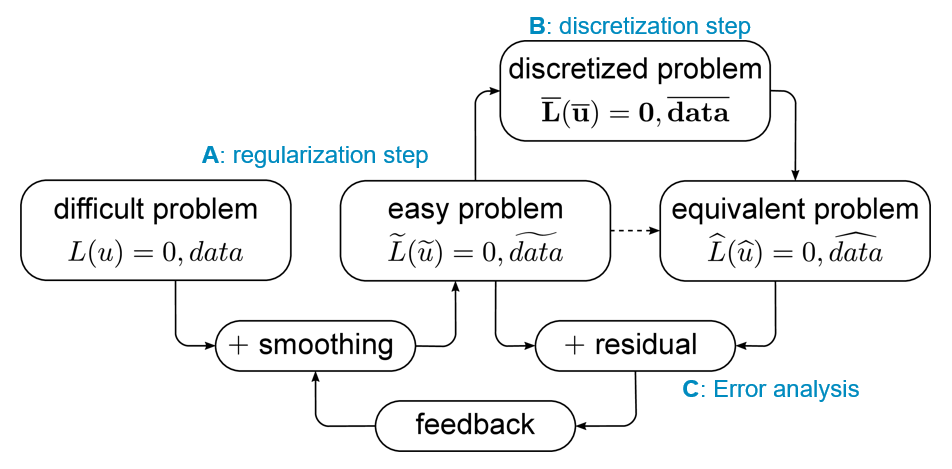
\includegraphics[width=0.9\textwidth]{figures/figure_1.png}
    \end{center}
    \caption{Graphical presentation of the error-minimizing two step method}\label{fig:two_step_method}
\end{figure}
%
Notation agreements:
\begin{symbollist}
    \item[$u$] Non-regularized/non-smoothed function, to be determined numerically.
    \item[$\widetilde u$] Regularized/smoothed function, denoted by the wavy line.
    \item[$\overline u$] Piecewise linear function, denoted by the bar.
    \item[$\widehat u$] Numerical solution on the nodes.
\end{symbollist}

A tilde ($\widetilde u$) indicates the variables and differential operators of the easy
problem.
Their discretizations are indicated by a bar, $\overline {u}$.
Next, we define the smooth and infinitely differentiable function $\widehat u$ that is a very close approximation of numerical solution $\overline {u}$.
By means of an error analysis we determine the differential problem that $\widehat u$ is a solution of.
Note that the data pertaining to the computational model are also included in the procedure.
Independent variables describing, e.g., the geometry and initial and boundary conditions also need to be discretized and hence need to be sufficiently smooth, to ensure that all higher-order error terms are sufficiently small and can be neglected.
Sufficient smoothness is obtained automatically by using smoothing coefficients that are a function of the discretization errors.
See also \citet{Borsboom2001}.


%%------------------------------------------------------------------------------
\chapter{Time integration scheme}\label{sec:time_integration}
To derive a time integration we start from the PDE:
\begin{align}
    \pdiff{\vec{u}}{t} + \vec{f}(\vec{u}) = 0\label{eq:pde}
\end{align}
%for the two dimensional linear wave  equations this equation reads
%\begin{align}
%    \pdiff{h}{t} + \pdiff{q}{x}  + \pdiff{r}{y}= 0
%    \\
%    \pdiff{q}{t} + gh\pdiff{\zeta}{x} = 0
%    \\
%    \pdiff{r}{t} + gh \pdiff{\zeta}{y} = 0
%\end{align}
For conservation types it can be written as:
\begin{align}
    \pdiff{\vec{u}}{t} + \nabla \dotp \vec{f}(\vec{u}) = \mat{S}
\end{align}
and when the finite volume approach is applied, we get
\begin{align}
    \int_\Omega \pdiff{\vec{u}}{t}\, d\Omega + \int_\Omega \nabla \dotp \vec{f}(\vec{u})\, d\Omega&= \int_\Omega \mat{S}\, d\Omega,
\end{align}
and after Green's theorem
\begin{align}
    \int_\Omega \pdiff{\vec{u}}{t}\, d\Omega + \int_\Gamma \vec{f}(\vec{u}) \dotp \vec{n}\, d\Gamma&= \int_\Omega \mat{S}\, d\Omega,
\end{align}
%--------------------------------------------------------------------------------
\section{Fully implicit time integration by adding an iteration process}\label{sec:fully_implicit}
The system of Equations \eqref{eq:pde} can be written as, including the $\theta$ method:
\begin{align}
    &\Dt_{inv} \mat{M} \left( \vec{u}^{n+1} - \vec{u}^{n} \right)  +
    \vec{f} \left( \vec{u}^{n+\theta} \right) = 0 \label{eq:discretized}
\end{align}
with $\Dt_{\it inv} = 1/\Dt$, $\mat{M}$ a mass-matrix and $0 \leq \theta \leq 1$.

To reach a fully implicit time integration an iteration process $p$ is added \citep[eqs.\ 15/16]{Borsboom2019a}:
\begin{align}
    &\Dt_{inv} \mat{M} \left( \vec{u}^{n+1,p+1} - \vec{u}^{n} \right)  +
    \vec{f} \left( \vec{u}^{n+\theta, p+1} \right) = 0
    \label{eq:1D_iteration}
\end{align}
iterating from $p \rightarrow p+1$ until convergence.

The \textbf{first} term is split to get a so called "Delta" formulation, taking into account the previous iteration:
\begin{align}
    &\Dt_{inv} \mat{M} \left( \vec{u}^{n+1,p+1} - \vec{u}^{n+1,p} + \vec{u}^{n+1,p} - \vec{u}^{n} \right) + \dots = 0
    \\
    & \Dt_{inv} \mat{M} \Delta \vec{u}^{n+1,p+1} + \dots  =
    - \Dt_{inv} \mat{M} \left( \vec{u}^{n+1,p} - \vec{u}^{n} \right)
\end{align}
with $\Delta \vec{u}^{n+1,p+1} = \vec{u}^{n+1,p+1} - \vec{u}^{n+1,p}$.
The right hand side is fully explicit (i.e.\ known at the previous iteration level $p$).
And if the iteration process is converged, the term at the left hand side is zero (i.e. $\Delta \vec{u}^{n+1,p+1} = 0$) so the right handside represent the time derivative.

The \textbf{second} term of \autoref{eq:discretized}
\begin{align}
    &\ldots +
    \vec{f} \left( \vec{u}^{n+\theta, p+1} \right) = 0
    \label{eq:second_term}
\end{align}
%
will be linearized around the iteration step $p$ (Newton linearization) and yields
\begin{align}
    \vec{f}( \vec{u}^{n+\theta, p+1} ) & = \vec{f}( \vec{u}^{n+\theta, p} ) + \pdiff{\vec{f}(\vec{u}^{n+\theta,p})}{\vec{u}^{n+1,p}} (\vec{u}^{n+\theta,p+1} - \vec{u}^{n+\theta,p})
    \\
    & = \vec{f}( \vec{u}^{n+\theta, p} ) + \pdiff{\vec{f}(\vec{u}^{n+\theta,p})}{\vec{u}^{n+1,p}} \Delta\vec{u}^{n+\theta,p+1} \label{eq:NewtonLinearization}
\end{align}
with
\begin{align}
    \Delta \vec{u}^{n+\theta, p+1} & = \vec{u}^{n+\theta, p+1} - \vec{u}^{n+\theta, p}
    \\
    & = \theta \vec{u}^{n+1, p+1} + (1-\theta) \vec{u}^{n} - \theta \vec{u}^{n+1, p} - (1-\theta) \vec{u}^{n}
    \\
    & = \theta \vec{u}^{n+1, p+1} - \theta \vec{u}^{n+1, p}
    \\
    &= \theta \Delta \vec{u}^{n+1, p+1} \label{eq:delta_n_theta}
\end{align}
After subtitution of \autoref{eq:delta_n_theta} into \autoref{eq:NewtonLinearization} we get:
\begin{align}
    \vec{f}( \vec{u}^{n+\theta, p+1} ) & = \vec{f}( \vec{u}^{n+\theta, p} ) + \theta \pdiff{\vec{f}(\vec{u}^{n+\theta,p})}{\vec{u}^{n+1,p}} \Delta \vec{u}^{n+1, p+1}
\end{align}
The Jacobian
\begin{align}
    \mat{J}^{n+1,p} & = \pdiff{\vec{f}(\vec{u}^{n+\theta,p})}{\vec{u}^{n+1,p}}
     = \pdiff{\vec{f}(\theta \vec{u^{n+1,p}} + (1 - \theta) \vec{u}^{n})}{\vec{u}^{n+1,p}}
\end{align}
is the approximate linearization of $\vec{f}$ as a
function of $\theta \vec{u}^{n+1} + (1-\theta)\vec{u}^{n}$ with respect to $\vec{u}^{n+1, p}$.
The Jacobians needed for the shallow water equations are described in \autoref{sec:jacobians}.


The total time integration method read:
\begin{empheq}[box=\fbox]{align}
    &\left(\Dt_{inv} \mat{M} + \theta\mat{J}^{n+1,p}\right)  \Delta \mat{u}^{n+1,p+1} =
    \nonumber \\
& \qquad = - \left( \Dt_{inv} \mat{M} \left( \vec{u}^{n+1,p} - \vec{u}^{n} \right) + \vec{f} \left( \theta \vec{u}^{n+1,p} + (1-\theta) \vec{u}^{n} \right) \right) \label{eq:Ax=b_b}
\end{empheq}
%
with $\vec{u}^{n+1,p+1}  = \vec{u}^{n+1,p} + \Delta \vec{u}^{n+1,p+1}$ and right hand side is explicit w.r.t.\  the iterator $p$.
In case the Newton iteration process converges, i.e.:
\begin{align}
    \lim_{p\rightarrow \infty}\left( \Delta \vec{u}^{n+1,p+1}\right) = \lim_{p\rightarrow \infty}\left( \vec{u}^{n+1,p+1} - \vec{u}^{n+1,p} \right) = 0.
\end{align}
%
then the left hand side of \autoref{eq:Ax=b_b} is equal to zero and thus it solves the original system of equations:
\begin{align}
    0 = \Dt_{inv} \mat{M} \left( \vec{u}^{n+1,p} - \vec{u}^{n} \right) + \vec{f} \left( \theta \vec{u}^{n+1,p} + (1-\theta) \vec{u}^{n} \right).
\end{align}
%
Because in the previous part we consider only the first derivative (Jacobian) and assumed that the second derivative is nearly zero, which is not always through.
Therefor we will extend the iteration process, see  \autoref{sec:pseudo_time_steppping}.
See also: \citet{Borsboom1998,Pulliam2014}


%--------------------------------------------------------------------------------
\subsection{Pseudo time stepping}\label{sec:psuedo_time_step}
\label{sec:pseudo_time_steppping}
In  \autoref{sec:fully_implicit} we assumed that only the Jacobian is relevant and the second derivative is negligible.
But in some case it is not the cases we have to assure that the following inequality is true:
\begin{align}
    \abs{ \half \frac{\partial^2 \vec{f}(\theta \vec{u}^{n+1,p}+ (1 - \theta)\vec{u}^n)}{(\partial \vec{u}^{n+1,p})^2} \Delta \vec{u}^{n+1,p+1}}
    < O\left(
    \abs{ \pdiff{\vec{f}(\theta \vec{u}^{n+1,p}+ (1 - \theta)\vec{u}^n)}{\vec{u}^{n+1,p} } }
    \right)
\end{align}
Therefor the time integration is extended with a (so called) pseudo timestep method, which read:
\begin{empheq}[box=\fbox]{align}
    & \left(\mat{M}_{pseu}\vec{T}^{n+1, p}_{pseu} + \Dt_{inv} \mat{M} + \theta\mat{J}^{n+1,p}\right)  \Delta \mat{u}^{n+1,p+1} =
    \nonumber \\
& \qquad = - \left( \Dt_{inv} \mat{M} \left( \vec{u}^{n+1,p} - \vec{u}^{n} \right) + \vec{f} \left( \theta \vec{u}^{n+1,p} + (1-\theta) \vec{u}^{n} \right) \right)
\end{empheq}
where $\vec{T}^{n+1, p}_{pseu}$ is a vector containing the inverse of the pseudo timestep, which may vary for all grid nodes, and $\mat{M}_{pseu}$ a mass-matrix operating on the pseudo timestep vector.
See for a more detailed description and how to choose the term $\mat{M}_{pseu}\vec{T}^{n+1, p}_{pseu}$
\citet{Borsboom2019a, Buijs2024}.

%--------------------------------------------------------------------------------
\section{Jacobians}\label{sec:jacobians}
As seen in \autoref{sec:fully_implicit} Jacobians need to be computed.
These Jacobians does not contain only derivatives to the major variables but also to place derivatives, which need special attention (\autoref{sec:jacobians_with_operator}).
For example for the two dimensional convection flux ($\vec{q}{\vec{q}^T}$) and presure term $gh\nabla \zeta$, where $\vec{q} = (q, r)^T$ and $\zeta$ the water level.

As example we take the integral form of the two dimensional non-linear wave equation.
This equation reads:
%
\begin{align}
    \int_\Omega \pdiff{\vec{u}}{t}\, d\Omega  + \int_\Omega \nabla \dotp \vec{F}\, d\Omega = 0
    \Leftrightarrow
    \int_\Omega \pdiff{\vec{u}}{t}\, d\Omega  + \oint_\Gamma \vec{F} \dotp \vec{n} \, d\Gamma = 0
\end{align}
with vector $\vec{u} = (h, q, r)^T$ the Jacobian read.
With
\begin{symbollist}
    \item[$h$] The total water depth, [$\si{\metre}$]
    \item[$q$] The water flux in $x$-direction, [$\si{\square\metre\per\second}$]
    \item[$r$] The water flux in $y$-direction, [$\si{\square\metre\per\second}$]
\end{symbollist}

The Jacobian of the function $F(h, q, r)$ as used in the two dimensional shallow water equations reads:
\begin{align}
    \mat{J} =
    \begin{pmatrix}
        J_{11} & J_{12} & J_{13} \\
        J_{21} & J_{22} & J_{23} \\
        J_{31} & J_{32} & J_{33}
    \end{pmatrix}
    =
    \begin{pmatrix}
        \pdiff{F_1}{h} & \pdiff{F_1}{q} &  \pdiff{F_1}{r} \\
        \pdiff{F_2}{h} & \pdiff{F_2}{q} &  \pdiff{F_2}{r} \\
        \pdiff{F_3}{h} & \pdiff{F_3}{q} &  \pdiff{F_3}{r}
    \end{pmatrix}
\end{align}


%--------------------------------------------------------------------------------
\subsection{Non-linear term, product}\label{sec:jacobians_with_non_linear_product_term}
If the Jacobian contains non-linear terms, each variable of $\vec{u}$ is linearized before using it in the non-linear term.
As an example a product of two quantities is taken, say $q$ and $r$ (like the convection term in two dimensional shallow water equations) and  $\Delta q^{n+1, p+1} = \Delta q$ and  $\Delta r^{n+1, p+1} = \Delta r$:
\begin{align}
    \left.(qr)\right|^{n+\theta, p+1} & = \left( q^{n+\theta, p} + \theta  \Delta q \right) \left( r^{n+\theta, p} + \theta  \Delta r\right) \approx
    \\
    & \approx  q^{n+\theta, p} r^{n+\theta, p} + \theta q^{n+\theta, p} \Delta r + \theta r^{n+\theta, p} \Delta q
\end{align}
omitting the quadratic term $O((\Delta q)^2, \Delta q \Delta r, (\Delta r)^2)$.
%--------------------------------------------------------------------------------
\subparagraph*{Jacobian}
When the Jacobian notation is  used for the function $F(q,r) = qr$
\begin{align}
    \mat{J} =
    \begin{pmatrix}
        J_{11} & J_{12}
    \end{pmatrix}
    =
    \begin{pmatrix}
        \pdiff{F}{q} & \pdiff{F}{r}
    \end{pmatrix}
    =
    \begin{pmatrix}
        \pdiff{qr}{q} & \pdiff{qr}{r}
    \end{pmatrix}
    =
    \begin{pmatrix}
        r & q
    \end{pmatrix}
\end{align}
 it leads to following approximation
\begin{align}
    \left.(qr)\right|^{n+\theta, p+1} &  \approx  q^{n+\theta, p} r^{n+\theta, p}+ \theta J_{11}^{n+\theta, p} \Delta q + \theta J_{12}^{n+\theta, p} \Delta r =
    \\
    & = q^{n+\theta, p} r^{n+\theta, p}+ \theta r^{n+\theta, p} \Delta q + q^{n+\theta, p} \Delta r
\end{align}

%--------------------------------------------------------------------------------
\subsection{Non-linear term, quotient}\label{sec:jacobians_with_non_linear_quotient_term}
If the Jacobian contains non-linear terms, each variable of $\vec{u}$ is linearized before using it in the non-linear term.
in this example a quotient of two quantities is taken, say $q$ and $h$ (representing the velocity in the two dimensional shallow water equations) and  $\Delta q^{n+1, p+1} = \Delta q$ and  $\Delta h^{n+1, p+1} = \Delta h$:
\begin{align}
    \left.\left(\frac{q}{h}\right)\right|^{n+\theta, p+1} & = \frac{ q^{n+\theta, p} + \theta  \Delta q }{ h^{n+\theta, p} + \theta  \Delta h} \approx
    \\
    & \approx \frac{ q^{n+\theta, p} + \theta  \Delta q }{ h^{n+\theta, p}} \left( 1 - \frac{\theta}{h^{n+\theta, p}} \Delta h  + O\left(  (\Delta h)^2 \right) \right)  \approx
    \\
    & \approx \left( \frac{ q^{n+\theta, p}}{ h^{n+\theta, p}} + \frac{\theta}{ h^{n+\theta, p}}  \Delta q \right)
    \left( 1 - \frac{\theta}{h^{n+\theta, p}} \Delta h  + O\left(  (\Delta h)^2 \right) \right)  \approx
    \\
    & \approx  \frac{ q^{n+\theta, p}}{ h^{n+\theta, p}}  - \theta \frac{ q^{n+\theta, p}}{ (h^{n+\theta, p})^2} \Delta h + \theta\frac{1}{ h^{n+\theta, p}}  \Delta q
\end{align}
omitting the quadratic term $O((\Delta q)^2, \Delta q \Delta h, (\Delta h)^2)$.
%--------------------------------------------------------------------------------
\subparagraph*{Jacobian}
When the Jacobian notation is  used for the function $F(h,q) = q/h$
\begin{align}
    \mat{J} =
    \begin{pmatrix}
        J_{11} & J_{12}
    \end{pmatrix}
    =
    \begin{pmatrix}
        \pdiff{F}{h} & \pdiff{F}{q}
    \end{pmatrix}
    =
    \begin{pmatrix}
        \pdiff{q/h}{h} & \pdiff{q/h}{q}
    \end{pmatrix}
    =
    \begin{pmatrix}
        -\frac{q}{h^2} & \frac{1}{h}
    \end{pmatrix}
\end{align}
it leads to following approximation
\begin{align}
    \left.(qr)\right|^{n+\theta, p+1} &  \approx  \frac{q^{n+\theta, p}}{r^{n+\theta, p}} + \theta J_{11}^{n+\theta, p} \Delta h + \theta J_{12}^{n+\theta, p} \Delta q =
    \\
    & = q^{n+\theta, p} r^{n+\theta, p} - \theta \frac{q^{n+\theta, p}}{(h^{n+\theta, p})^2} \Delta h + \theta \frac{1}{h^{n+\theta, p}} \Delta q
\end{align}
%--------------------------------------------------------------------------------
\subsection{Terms with an operator}\label{sec:jacobians_with_operator}
The Jacobian of an operator is also applied to the argument of the operator.
As an example the pressure term of the shallow water equations is taken, where $\Delta h^{n+1, p+1} = \Delta h$ and  $\Delta \zeta^{n+1, p+1} = \Delta \zeta$:
\begin{align}
    \left. gh \pdiff{\zeta}{x}\right|^{n+\theta, p+1} & \approx g \left( h^{n+\theta, p} + \theta \Delta h \right) \pdiff{}{x} \left( \zeta^{n+\theta, p} + \theta\Delta \zeta  \right) \approx
%    & = g h^{n+\theta, p} \pdiff{\zeta^{n+\theta, p}}{x} + gh^{n+\theta, p} \pdiff{\theta\Delta \zeta}{x} + g \theta\Delta h \pdiff{\zeta^{n+\theta, p}}{x} + O(\Delta h \Delta \zeta) \approx
%    \\
%    & \approx g h^{n+\theta, p} \pdiff{\zeta^{n+\theta, p}}{x} + gh^{n+\theta, p} \pdiff{\theta\Delta \zeta}{x} + g \pdiff{\zeta^{n+\theta, p}}{x} \theta\Delta h =
    \\
    & \approx g h^{n+\theta, p} \pdiff{\zeta^{n+\theta, p}}{x} + \theta gh^{n+\theta, p} \pdiff{\Delta \zeta}{x} + \theta g \pdiff{\zeta^{n+\theta, p}}{x} \Delta h
\end{align}
omitting the quadratic  term $O(\Delta h\ \lpdiff{\Delta \zeta}{x})$.
The term  $\lpdiff{\Delta \zeta}{x}$ is not always small and therefor a psuedo time step method is introduced, see \autoref{sec:psuedo_time_step}.
In discrete form it reads on location $x_{i+\half}$:
\begin{align}
    \left. gh \pdiff{\zeta}{x}\right|^{n+\theta, p+1}_{i+\half} & \approx g h^{n+\theta, p}_{i+\half} \frac{\zeta^{n+\theta, p}_{i+1} - \zeta^{n+\theta, p}_{i}}{\Dx_{i}}
    + \theta gh^{n+\theta, p}_{n+\half} \frac{\Delta \zeta_{i+1} - \Delta \zeta_{i}}{\Dx_{i}} +
    \\
    & \quad
    + \theta g \frac{\zeta^{n+\theta, p}_{i+1} - \zeta^{n+\theta, p}_{i}}{\Dx_{i}} \Delta h_{i+\half}
\end{align}
Remember that the gradient over a grid cell $\Dx_i$ is constant, due to the piecewise linear approximation between two nodes.
%--------------------------------------------------------------------------------
\subparagraph*{Jacobian}
When the Jacobian notation is  used for the function $F(q,h) = gh\, \lpdiff{\zeta}{x}$
\begin{align}
    \mat{J} =
    \begin{pmatrix}
        J_{11} & J_{12}
    \end{pmatrix}
    =
    \begin{pmatrix}
        \pdiff{F}{h} & \pdiff{F}{\zeta}
    \end{pmatrix}
    =
    \begin{pmatrix}
        \pdiff{(gh\, \lpdiff{\zeta}{x})}{h} & \pdiff{(gh\, \lpdiff{\zeta}{x})}{\zeta}
    \end{pmatrix}
    =
    \begin{pmatrix}
        g\, \pdiff{\zeta}{x} & gh\, \pdiff{}{x}
    \end{pmatrix}
\end{align}
it leads to following approximation
\begin{align}
    \left.gh \pdiff{\zeta}{x}\right|^{n+\theta, p+1}_{i+\half} & \approx g h^{n+\theta, p} \pdiff{\zeta^{n+\theta, p}}{x}  + \theta J_{11}\Delta h  + \theta J_{12} \pdiff{}{x}(\Delta \zeta) \approx
    \\
    & \approx g h^{n+\theta, p} \frac{\zeta^{n+\theta, p}_{i+1} - \zeta^{n+\theta, p}_{i}}{\Dx_{i}}
    + \theta g \frac{\zeta^{n+\theta, p}_{i+1} - \zeta^{n+\theta, p}_{i}}{\Dx_{i}} \Delta h_{i+\half} +
    \\
    & \quad + \theta gh^{n+\theta, p}_{n+\half} \frac{\Delta \zeta_{i+1} - \Delta \zeta_{i}}{\Dx_{i}}
\end{align}

%%------------------------------------------------------------------------------
\chapter{1-D Space discretization}\label{sec:1d_space_discretization}
We are looking for a second order central space discretization together with the finite volume approach.
So the higher order terms in the Taylor series expansion are negligible.
For this numerical discretization method no dissipation is added, only there is some dispersion for the shorter waves, i.e.\ dependent on the third derivative in the Taylor expansion.
To fulfill this requirement the data should be smooth according to the truncation error of the numerical discretization.
If not, the data should be made smooth with a procedure in which you can see on which location the smoothing is severe.
The process of smoothing is called regularization.
If the truncation error (high values of second derivatives) is severe on locations that the user do not expect and do not accept then the user can adjust the discretization in that part of the domain.
%
There are two options to adjust the data:
\begin{enumerate}
    \item increase the smoothing coefficient or
    \item choose a smaller grid size.
\end{enumerate}

%------------------------------------------------------------------------------
\section{Finite volume approach}
We will discuss the finite volume approach for the one dimensional case of the function $u(x,t)$,
for the grid shown in  \autoref{fig:water_body_fve_bc_at_node}
\begin{figure}[H]
    \centering
    \begin{center}
    \resizebox{0.8\textwidth}{!}{
        \input{figures/water_body_fve_bc_at_node.pdf_tex}
    }
\end{center}
    \caption{Water body (blue area), finite volumes (green boxes), computational points (open dots), virtual computational points (black dots), boundary points (open squares) are at $i=1$ (west boundary) and $i=I$ (east boundary).}\label{fig:water_body_fve_bc_at_node}
\end{figure}
The control volume is defined on the interval $x_{i-\half}$ to $x_{i+\half}$, see \autoref{fig:water_body_fve_bc_at_node}.
The grid in \autoref{fig:water_body_fve_bc_at_node} is equidistant but that is not necessarily, the method which is described in this document also holds for a non-equidistant grid.

%------------------------------------------------------------------------------
\subsection{Quadrature rule, source term}\label{sec:source_quadrature_rule}
The finite volume approach for the function $u(x,t)$ reads:
\begin{align}
    \int_\Omega u \, d\Omega = \int_{x_{i-\half}}^{x_{i+\half}} u \, dx
\end{align}
Using piecewise linear functions between the non-equidistant nodes the quadrature rule reads:
\begin{align}
    \int_{x_{i-\half}}^{x_{i+\half}} u \, dx & = \int_{x_{i-\half}}^{x_i} u \, dx + \int_{x_i}^{x_{i+\half}} u \, dx \approx
    \\
    & \approx \frac{\Dx_{i-\half}}{2} \frac{u_{i-1} + 3 u_{i}}{4} + \frac{\Dx_{i+\half}}{2} \frac{3 u_{i} + u_{i+1}}{4} \label{eq:integral_control_volume}
\end{align}
where the control volume is split into two adjacent sub-control volumes  $[x_{i-\half}, x_i]$ and $[x_i, x_{i+\half}]$.
A graphical interpretation is given in \autoref{fig:1d_integration}.
\begin{figure}[H]
    \begin{center}
        \resizebox{0.8\textwidth}{!}{
            \input{figures/1d-integration.pdf_tex}
        }
    \end{center}
    \caption{Integration at $x_i$ over the control volume from $x_{i-\half}$ to $x_{i+\half}$.}\label{fig:1d_integration}
\end{figure}
Higher order quadrature rules may be chosen, but they are not discussed in this report.
%------------------------------------------------------------------------------
\subsection{Quadrature rule, flux term}\label{sec:flux_quadrature_rule}

%------------------------------------------------------------------------------
\subsection{Boundary conditions}\label{sec:boundary_conditions}
At the west and east boundary boundary conditions need to be supplied.
If it is a prescribed boundary condition (ingoing signal) it is called an \textbf{essential}-boundary condition, if the boundary condition is determined by the outgoing signal it is called a \textbf{natural}-boundary condition \citep{Logan1987,VanKanEtAL2008}.
In case of a wave equation we have a right and left going signal.
When no reflection at an open boundary is required then at the west boundary a signal need to prescribed  without disturbing the left going signal.
And at the east boundary the other way around.

Further more we have the prescribed boundary signal at the boundary node of the grid.
This assumption is made because user are acquitained with the fact that open boundaries are given at nodes.
But for the outgoing signal this is not necessarily, for the outgoing signal we stick to the finite volume approach.

When we first consider a right going one dimensional advection equation (see \autoref{sec:1d_advection_equation}) the boundary at the west side is located at $x_1$ and the outflow condition is located at $x_{I+\half}$.
The prescribed function reads:
\begin{align}
    c(0,t) = f(t)
\end{align}
Because we use a 3-point stencil for the interior, we aim for a 3-point stencil for the essential boundary condition.
One possible quadratic interpolation is a parabolic fit through the grid points, giving an underspecification of the solution at the boundary regardless of its position.
\begin{align}
    c_{GP}(\xi) & = c_0 \,  (1 - \xi) + c_1 \,  \xi + \half(c_0 - 2\, c_1 + c_2) \,  (\xi - 1) \,  \xi
    =
    \nonumber \\
    & =  \left(1 - \xi\right) \,  \left(1 - \half \xi\right) c_0  + \xi \,  \left(2 - \xi\right) c_1 + \half \xi  \left(\xi - 1\right) \,  c_2
    \label{eq:20231214-1}
\end{align}
where $\xi\in [0,1]$ is the weight function between $c_0$ and $c_1$.

Another possible quadratic fit is the one through Cell-Centered values:
\begin{align}
    c_{CC}(\xi) & = c_0 \, \left(1 - \xi\right) + c_1\,  \xi + \half (c_0 - 2c_1 + c_2) \,   \left(\xi - \half\right)^2
    \\
    & = \left( 1 - \xi + \half \left(\xi - \half\right)^2 \right) c_0 +
    \left( \xi - \left(\xi - \half\right)^2  \right) c_1  +
    \left(   \half \left(\xi - \half\right)^2\right) c_2       \label{eq:20231214-5}
\end{align}
The parabolic fit that gives neither underspecification nor overspecification of
imposed values at boundaries is a combination of Equation (45) and (49). It is easy to show
that that combination consists of $1/3$ times \autoref{eq:20231214-1} plus $2/3$ times \autoref{eq:20231214-5}:
\begin{align}
    c_{opt}(\xi) & = \left( \frac{13}{12} - \frac{3}{2}\xi - \half \xi^2 \right) c_0 +
    \left( -\frac{1}{6} + 2 \xi - \xi^2 \right) c_1  +
    \left( \frac{1}{12} - \half \xi +  \half \xi^2  \right) c_2       \label{eq:20231214-5}
\end{align}
Which lead to the following interpolations for $\xi=\half$ and $\xi=1$:
\begin{align}
    c_{opt}\left(\half\right) & = \frac{11}{24} c_0 + \frac{14}{24} c_1 - \frac{1}{24} c_2 \label{eq:stencil_nat}
    \\
    c_{opt}\left(1\right)  & = \frac{1}{12} c_0 + \frac{10}{12} c_1 + \frac{1}{12}c_2 \label{eq:stencil_ess}
\end{align}
Where \autoref{eq:stencil_nat} will be used for the natural boundary condition and \autoref{eq:stencil_ess} will be used for the essential boundary condition.

Verification of its correctness by means of integration over the outermost finite volume:
\begin{align}
\int_{\xi_{\half}}^{\xi_{\frac{3}{2}}} c_{opt}(\xi)\, d\xi = \frac{1}{8} c_0 + \frac{3}{4} c_1 + \frac{1}{8} c_2
\end{align}
In the right-hand side we see the weights of the mass matrix of the piecewise linear FVE
method, i.e.\ averaged over the left outermost finite volume the quadratic function $c_{opt}$
equals the piecewise linear function used in the FVE scheme.
%------------------------------------------------------------------------------
%\newpage
\section{Regularization of artificial viscosity $\mathbf{\Psi}$}\label{sec:regularization_artificial_viscosity}
To get an error-minimizing method we need to regularize all data, as mentioned in \autoref{sec:error_minimizing}.
Regularization of the artificial viscosity $\Psi$ is performed as described in \citet[eq.\ 14]{Borsboom2001}.
\begin{align}
    \int_\Omega \Psi\, d\omega - \alpha \int_\Omega \Dxi^2 \pdiff[2]{\Psi}{\xi}\, d\omega = \int_\Omega c_{\psi} Err_\Psi\, d\omega
\end{align}
%\todo{Which value of $\alpha$ need to be used and why?}
When discretized it yields \citep[eq.\ 18]{Borsboom2001}:
\begin{align}
    \left(\frac{1}{8} - \alpha \right)\Psi_{i-1} + 
    \left(\frac{3}{4} + 2\alpha \right)\Psi_{i} + 
    \left(\frac{1}{8} - \alpha \right)\Psi_{i+1} = \frac{c_{\Psi}}{\Dxi} \int^{\xi_{i+\half}}_{\xi_{i-\half}} Err_{\Psi}\, d\xi
    \label{eq:discrete_regularization_psi}
\end{align}
%\todo{Where is this equation coming from (energy equation?), derivation/explanation needed.}
%Dimension analysis:
%\begin{align}
%\si{[\square\metre\per\second]} = [1] [m] \left(  \sqrt{\frac{\si{[\metre\per\square\second]}}{\si{[\metre]}}} \si{[\metre]}
%    + \frac{1}{\si{[\metre]}} \si{[\square\metre\per\second]} 
%    - \frac{ \si{[\square\metre\per\second]}}{\si{[\square\metre]} } \si{[\metre]}
%    \right)
%\end{align}
%
The right hand side of \autoref{eq:discrete_regularization_psi} can be approximated by:
\begin{align}
    \frac{c_{\Psi}}{\Dxi} \int^{\xi_{i+\half}}_{\xi_{i-\half}} Err_{\Psi}\, d\xi 
& =
    \frac{c_{\Psi}}{\Dxi} \int^{\xi_{i}}_{\xi_{i-\half}} Err_{\Psi}\, d\xi 
    + \frac{c_{\Psi}}{\Dxi} \int^{\xi_{i+\half}}_{\xi_{i}} Err_{\Psi}\, d\xi \approx 
    \\*
    &\approx \frac{c_{\Psi}}{\Dxi} \frac{1}{2\Dxi} (Err_{\Psi})_{i-\quart} 
  + \frac{c_{\Psi}}{\Dxi} \frac{1}{2\Dxi} (Err_{\Psi})_{i+\quart}
%    \approx \frac{c_{\Psi} }{\Dxi}  (Err_{\Psi})_{i}
%    &\approx c_{\Psi} \left( \frac{1}{8} (Err_{\Psi})_{i-1}+ \frac{6}{8}  (Err_{\Psi})_{i} + \frac{1}{8}   (Err_{\Psi})_{i+1} \right)
%\\*
%&\approx \frac{c_{\Psi} }{2 \Dxi}  \left( (Err_{\Psi})_{i+1} - (Err_{\Psi})_{i-1} \right) 
\end{align}
For $Err_\Psi$ the following expression is used (\citet[eq.\ 42]{Borsboom2001}, a derivation of this expression is given in \autoref{sec:error_artificial_viscosity}):
\begin{align}
    &Err_\Psi = \Dxi\, \overline{x}_\xi \left( \half \sqrt{\frac{g}{\hbar}} \abs{D_\xi(\overline\zeta)} + 
    \half \sqrt{2} \abs{\frac{D_\xi(\qbar)}{\hbar} - \frac{\qbar D_\xi(\hbar)}{\hbar^2}} \right)
\end{align}
using (with $\ubar \in \{\hbar, \qbar\}$):
\begin{align}
    \ubar_{i-\quart} = \quart(u_{i-1} + 3 u_{i}), \qquad \ubar_{i+\quart} = \quart(u_{i+1} + 3 u_{i})
\end{align}
and
\begin{align}
    {(\overline{x}_{\xi})}_{i-\quart}= x_i - x_{i-1}, \qquad 
    {(\overline{x}_{\xi})}_{i+\quart}= x_{i+1} - x_{i}
\end{align}
and for equidistant meshes we use \citep[eq.\ 35]{Borsboom2001} :
\begin{align}
    D_\xi(\ubar) = \Dxi^2 \pdiff[2]{}{\xi} \approx u_{i-1} - 2 u_{i} + u_{i+1}.
\end{align}
\phantom{text}
%\todo{Find the correct approximation}



%------------------------------------------------------------------------------
\section{Regularization of given function}
To get an error-minimizing method we need to regularize all data, as mentioned in \autoref{sec:error_minimizing}.
Regularization of a given function is performed as described in \citet{Borsboom1998} and \citet{Borsboom2003}.
The given function to regularize reads:
\begin{align}
    u_{giv}(x).
\end{align}
Some notation agreements are:
\begin{symbollist}
    \item[$u$] Non-regularized/non-smoothed function, to be determined numerically.
    \item[$\widetilde u$] Regularized/smoothed function, denoted by the wavy line.
    \item[$\overline u$] Piecewise linear function, denoted by the bar.
    \item[$u_i$] Value of the numerical value at point $x_i$, denoted by the subscript.
\end{symbollist}

The regularized function $\widetilde u$ satisfy the next equation \citep[eq.\ 6]{Borsboom1998}:
\begin{align}
    \widetilde u - \pdiff{}{x} \Psi \pdiff{\widetilde u}{x} = u_{giv}, \qquad \Psi = c_{\Psi}\Delta x^2 E, \label{eq:regularization}
\end{align}
where
\begin{symbollist}
    \item[$u_{giv}$] Given function, ex.\ bathymetry, viscosity, \ldots, [\si{\cdot}].
    \item[$\widetilde u$] Regularized/smoothed function of $u_{giv}$, [\si{\cdot}].
    \item[$\Psi$] (Artificial) smoothing coefficient, [\si{\square\metre}]
    \item[$\Dx$] Space discretization, $\Dx_{i+\half} = x_{i+1} - x_{i}$, [\si{\metre}]
    \item[$c_{\Psi}$] Smoothing factor (set by user), [\si{1/\cdot}]
    \item[$E$] Error function, [\si{\cdot}] (see \autoref{sec:determine_psi})
\end{symbollist}


First the discretization of \autoref{eq:regularization} is discussed and second the determination of the artificial smoothing coefficient $\Psi$.

The finite volume approach of \autoref{eq:regularization} reads:
\begin{align}
\int_\Omega \widetilde u\, d\Omega  - \int_\Omega \pdiff{}{x}  \Psi \pdiff{\widetilde u}{x}\, d\Omega  = \int_\Omega  u_{\it{giv}}\, d\Omega \label{eq:1d_regularization}
\end{align}
%--------------------------------------------------------------------------------
\paragraph*{Integration of the first term}
Integration of the first term yields: %, see \autoref{sec:integration_1d_controle_volume}.
\begin{align}
\int_{x_{i-\half}}^{x_{i+\half}} \widetilde u\, dx \approx
\half \Dx_{i-\half} \left( \frac{1}{4} u_{i-1} + \frac{3}{4} u_{i} \right)  +
\half \Dx_{i+\half} \left( \frac{3}{4} u_{i} + \frac{1}{4} u_{i+1} \right)
\end{align}
%--------------------------------------------------------------------------------
\paragraph*{Integration of the second term}
Integration of the second term, with $\Psi_{i+\half} = \half(\Psi_{i} + \Psi_{i+1})$:
\begin{align}
\int_{x_{i-\half}}^{x_{i+\half}} &\, \pdiff{}{x} \Psi \pdiff{\widetilde u}{x} dx  =
\left. \Psi \pdiff{\widetilde u}{x} \right|_{i+\half} -  \left. \Psi \pdiff{\widetilde u}{x} \right|_{i-\half} \approx \\
& \approx \Psi_{i+\half} \frac{ u_{i+1} -  u_{i}}{\Dx_{i+\half}} - \Psi_{i-\half} \frac{ u_{i} -  u_{i-1}}{\Dx_{i-\half}} = \\
%        & = - \frac{\nu^h_{i-\half}}{\Dx_{i-\half}}  u_{i-1} +  \frac{\nu^h_{i-\half}}{{\Dx_{i-\half}}}  u_{i} +  \frac{\nu^h_{i+\half}}{{\Dx_{i+\half}}}  u_{i} - \frac{\nu^h_{i+\half}}{{\Dx_{i+\half}}}  u_{i+1} \\
&=  \frac{\Psi_{i-\half}}{\Dx_{i-\half}}   u_{i-1}
-  \left( \frac{\Psi_{i-\half}}{{\Dx_{i-\half}}}
+  \frac{\Psi_{i+\half}}{{\Dx_{i+\half}}} \right)  u_{i}
+ \frac{\Psi_{i+\half}}{{\Dx_{i+\half}}}   u_{i+1}
\end{align}
%--------------------------------------------------------------------------------
\paragraph*{Integration of the right hand side}
For the integration of the right hand side we could use a smaller integration step size, to incorporate the sub-grid scale effects.
If the function $u_{giv}$ is for example an analytic function this integral can be computed exact or data is given by a lot of measurement points per finite volume, see for example \autoref{fig:subgrid_scale_2d}.
When integrating over a finite volume the sub-grid scale effects will be taken into account
\begin{figure}[H]
    \centering
    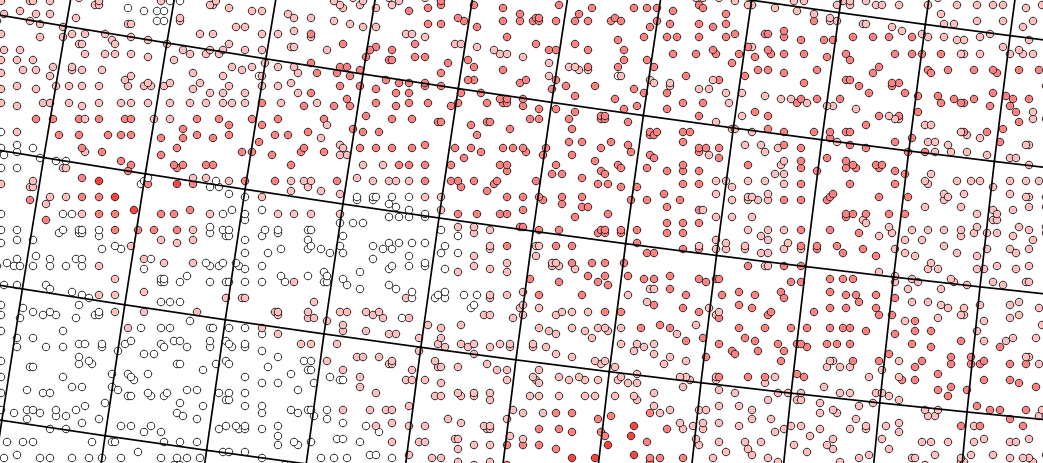
\includegraphics[width=0.9\textwidth]{figures/subgrid_scale_2d.png}
    \caption{Two dimensional example of a lot of data points per grid cell. The data points are used to compute the integral at the righthand side of \autoref{eq:disc_regularization}. \label{fig:subgrid_scale_2d}}
\end{figure}

%--------------------------------------------------------------------------------
\paragraph*{Discretization of \autoref{eq:1d_regularization}}
So the discretization of \autoref{eq:1d_regularization} with $\alpha = \frac{1}{8}$, read (i.e.\ \citet[eq.\ 7]{Borsboom1998} and \citet[eq.\ 6]{Borsboom2003}):
\begin{align}
\left( \frac{\Dx_{i-\half}}{8}
- \frac{\Psi_{i-\half}}{\Dx_{i-\half}} \right)  u_{i-1} &
+ \left( \frac{3\Dx_{i-\half}}{8}  + \frac{\Psi_{i-\half}}{{\Dx_{i-\half}}}  + \frac{3\Dx_{i+\half}}{8} +  \frac{\Psi_{i+\half}}{{\Dx_{i+\half}}} \right)  u_i +
\\
& + \left(  \frac{\Dx_{i+\half}}{8} - \frac{\Psi_{i+\half}}{{\Dx_{i+\half}}} \right)  u_{i+1}  = \int_{x_{i-1/2}}^{x_{i+\half}} u_{giv}\, dx
\label{eq:disc_regularization}
\end{align}
The boundary conditions to close the three diagonal system are $u_0  = {u_{giv}}(x_{0})$ and $u_{I+1} = {u_{giv}}(x_{I+1})$.

%--------------------------------------------------------------------------------
\subsection{Determination of artificial smoothing coefficient $\Psi$}\label{sec:determine_psi}
The artificial smoothing coefficient $\Psi$ ( $ = c_{\psi} \Dx^2 E$, \autoref{eq:regularization}) is dependent on error $E$, the smoothing coefficent $c_E$ and the second derivative of the given function $u_{giv}$ \citep[eq.\ 8]{Borsboom1998}.
The error $E$ will be computed in computational space, meaning that a disturbance is spreaded over an equal number of cells before and after the location of the disturbance:
%
\begin{align}
    &\left(\frac{\Dxi}{8}-\frac{c_E}{\Dxi}\right) E_{i-1} + \left(\frac{6\Dxi}{8} + \frac{2c_E}{\Dxi}\right) E_i + \left(\frac{\Dxi}{8} - \frac{c_E}{\Dxi}\right)E_{i+1}
    =  \int_{\xi_{i-\half}}^{\xi_{i+\half}} \abs{D_i} \, d\xi
    \label{eq:error_regularization}
\end{align}
with $\Dxi =1$ it reads:
\begin{align}
    &\left(\frac{1}{8}-c_E\right) E_{i-1} + \left(\frac{6}{8} + 2c_E\right) E_i + \left(\frac{1}{8} - c_E\right)E_{i+1}
    =   \abs{D_i}
    \label{eq:error_regularization}
\end{align}
\textbf{Choose $\mathbf{c_E}$ equal to $\mathbf{c_{\psi}}$} and take into account that $D_i$ is constant over a control volume
\begin{align}
    D_i & = \Dxi^2 \pdiff[2]{u_{giv}}{\xi} \quad \text{ \citep[eq.\ 2]{Borsboom1998}}
    \\ & \approx {u_{giv}}_{i-1} - 2 {u_{giv}}_{i-1} + {u_{giv}}_{i+1}
\end{align}
%
Now system the system of \autoref{eq:error_regularization} can be solved and where $\vec{\Psi}$ is set to:
\begin{align}
    \vec{\Psi} = c_{\Psi}\Dx^2 \vec{E}
\end{align}
For an estimation of $c_{\Psi}$ see \autoref{sec:determine_factor_c_psi}, in this document we use $c_{\Psi} = 4$.

The boundary conditions to close the three diagonal system are:
\begin{align}
    2 E_0 - E_1 & = \abs{D_{1}} \quad \text{and}
    \\
    - E_{I} + 2 E_{I+1} & = \abs{D_{I}}.
\end{align}

%--------------------------------------------------------------------------------
\subsection{Step function (Heaviside function)}
For a full description of this example see \citet[eq.\ 5]{Borsboom2003}.
The function is initially defined as:
\begin{align}
    u_{given}(x) =
    \begin{cases}
        0, & \text{if} \quad 0\ [m] \leq x \leq 1000\ [m],
        \\
        1, & \text{if} \quad 1000\ [m] < x \leq 2000 \ [m],
    \end{cases}
\end{align}
For illustration, the step is chosen to be exactly on a grid point (in the middle of a control volume at $1000\ [m]$) and at the finite volume boundary, i.e.\ a half $\Dx$ shifted to the right.
\begin{figure}[H]
    \centering
    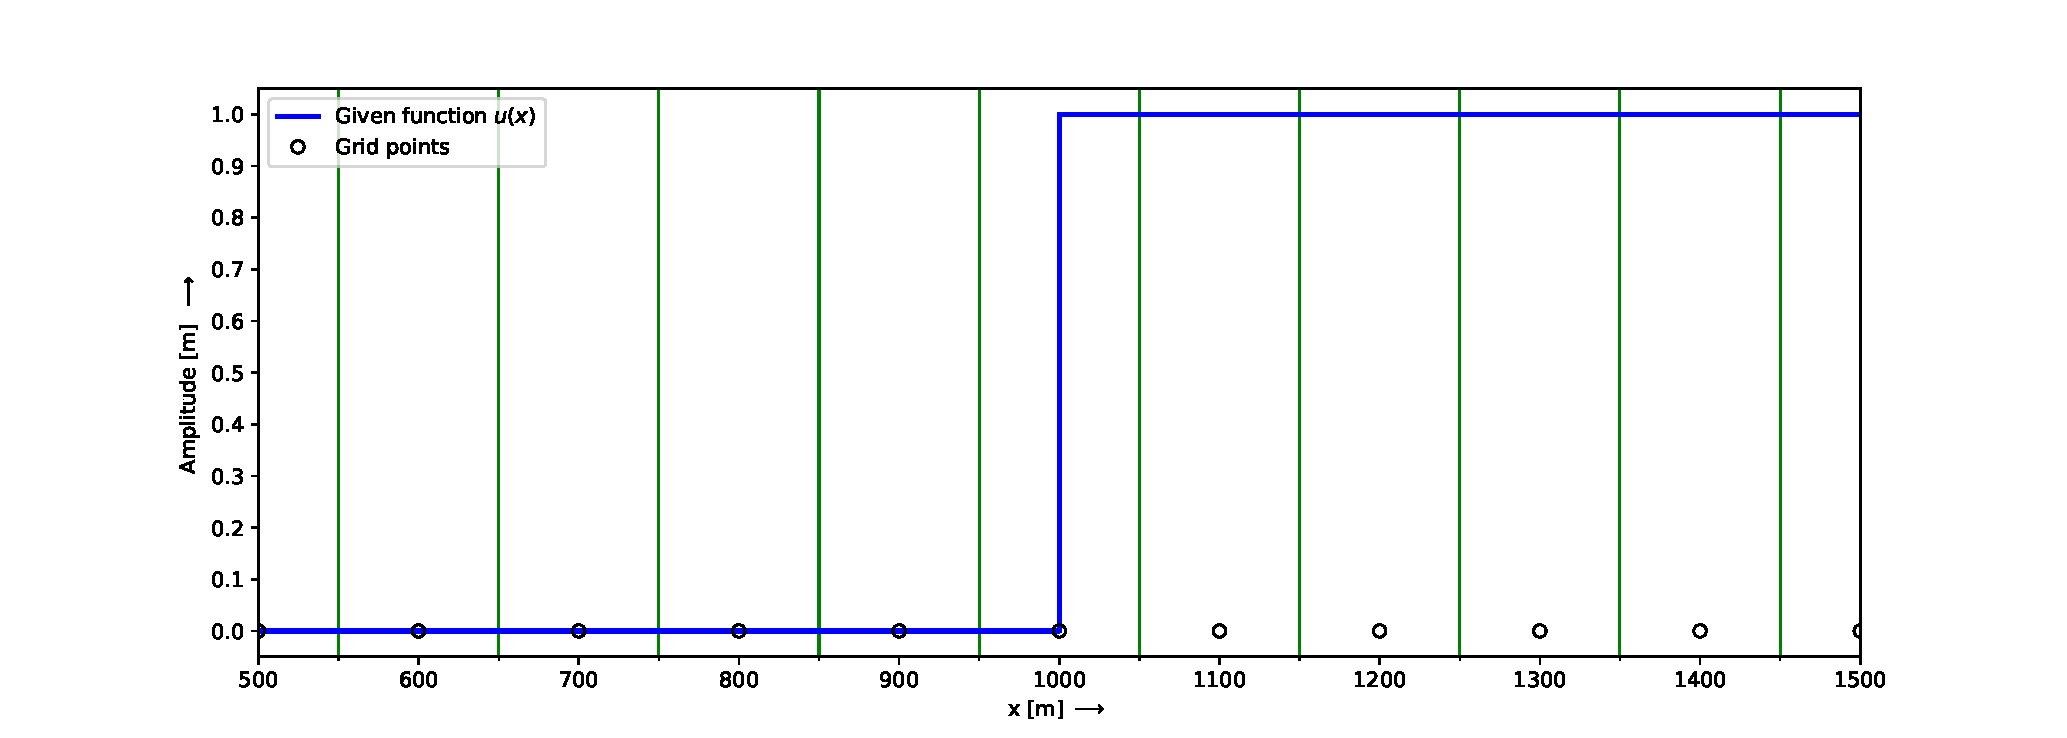
\includegraphics[width=1.0\textwidth]{figures/1d_step_function_dx100.pdf}
    \caption{Step function to be estimated. The thin green vertical lines indicate the  borders of the finite volumes.\label{fig:ex_step_function}}
\end{figure}
A straight forward piecewise approximation is shown in \autoref{fig:straight_forward_discretization}.
Both figures does show the same discretization function (cyan colored) but the step is at a different location.
%
\begin{figure}[H]
    \centering
    \begin{subfigure}[t]{0.49\textwidth}
        \centering
        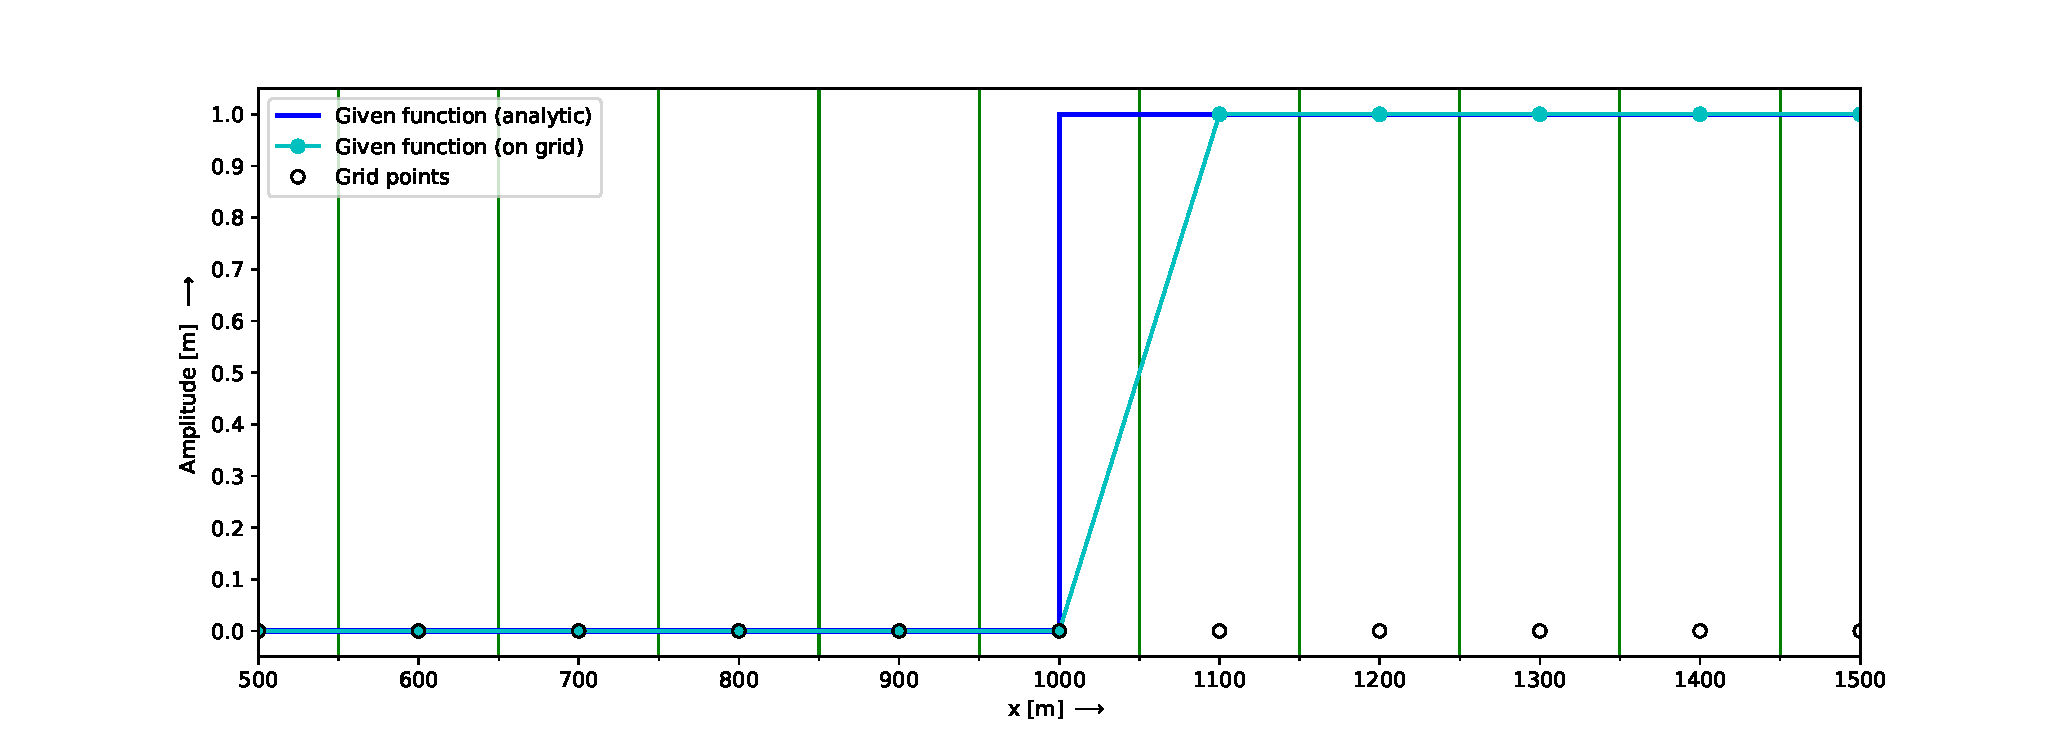
\includegraphics[width=1.0\textwidth]{figures/regul_1_1d_scalar_dx100.pdf}
        \caption{Step at grid node, $x = 1000\ [m]$}
    \end{subfigure}
    \hfill
    \begin{subfigure}[t]{0.49\textwidth}
        \centering
        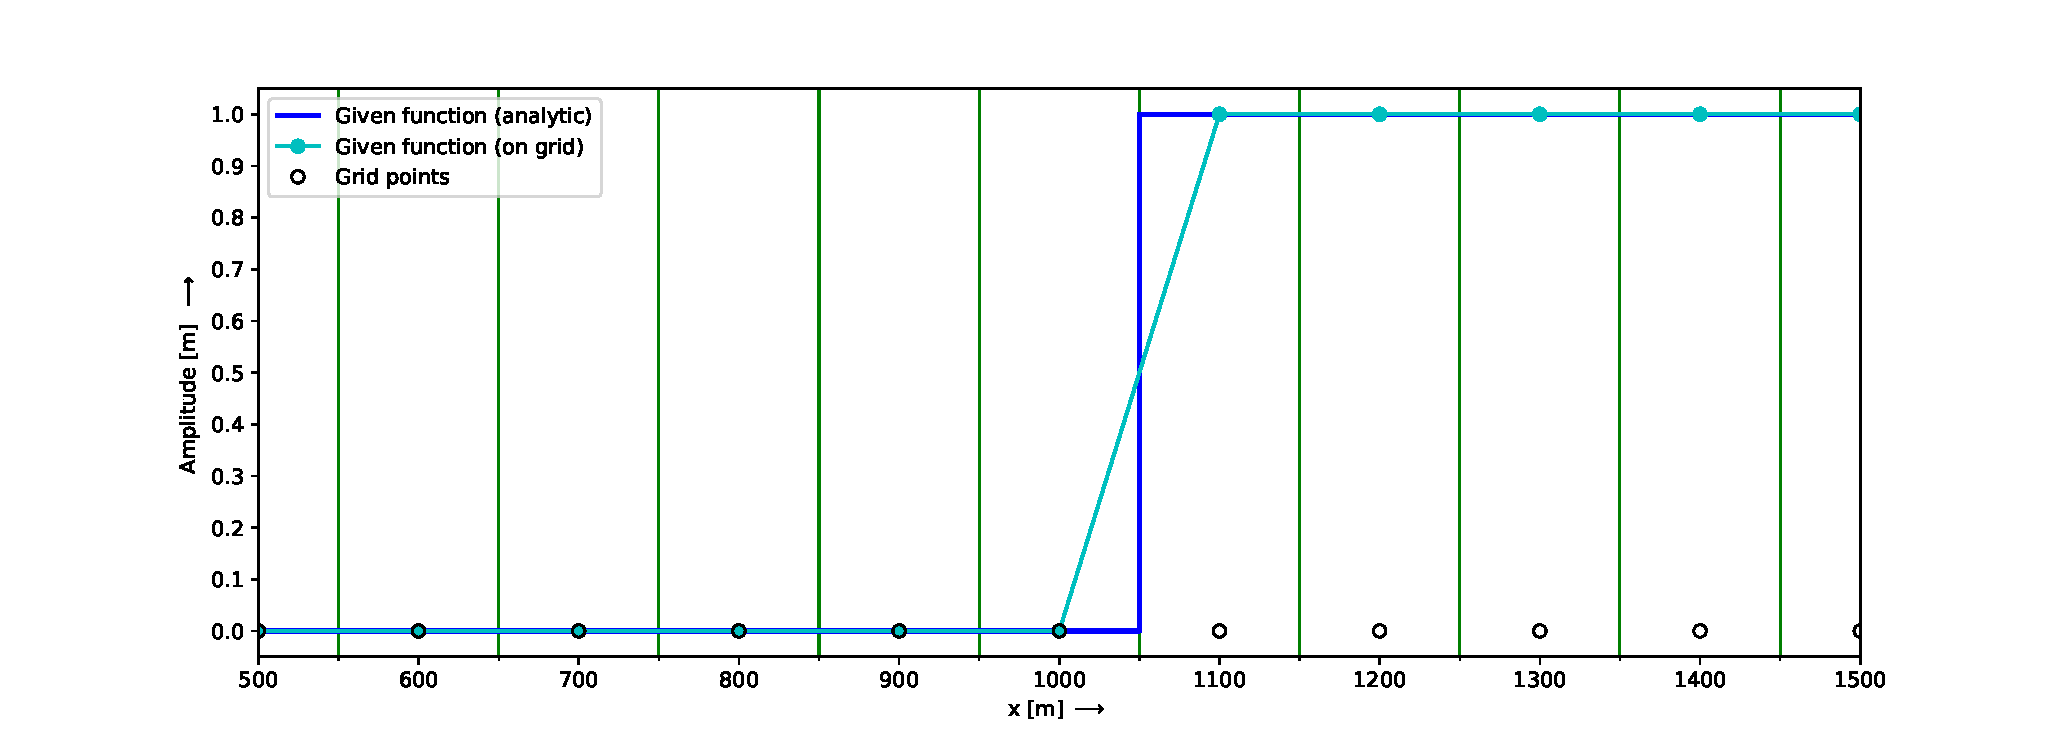
\includegraphics[width=1.0\textwidth]{figures/regul_2_1d_scalar_dx100.pdf}
        \caption{Step at boundary of a finite volume, $x = 1050\ [m]$}
    \end{subfigure}
    \caption{As seen from this figures the function defined on the grid nodes does not see the exact location of the step. Both function through the grid nodes have the same profile, but the step is at another location. \label{fig:straight_forward_discretization}}
\end{figure}
%
A piecewise approximation with a regularization coefficient of zero ($c_\Psi = 0$) is shown in \autoref{fig:ex_step_function_no_regularization}.
%
\begin{figure}[H]
    \centering
    \begin{subfigure}[t]{0.49\textwidth}
        \centering
        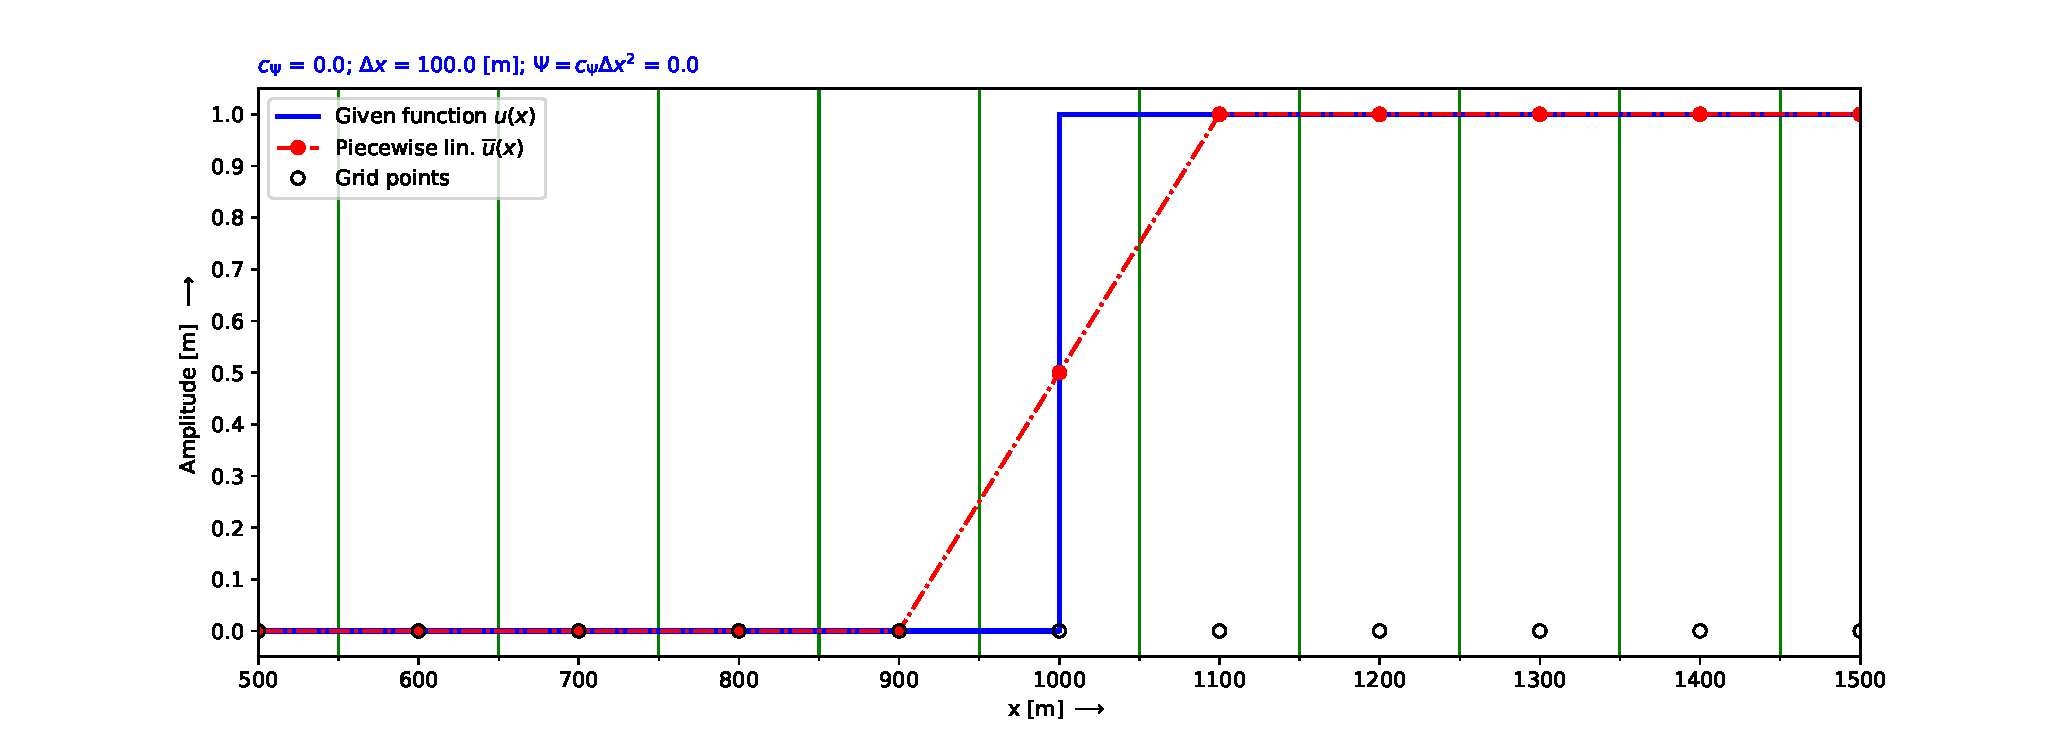
\includegraphics[width=1.0\textwidth]{figures/regul_1_1d_step_function_dx100.0_cpsi1e-06.pdf}
        \caption{Step at grid node, $x = 500\ [m]$}\label{fig:ex_step_function_no_regularization_a}
    \end{subfigure}
    \hfill
    \begin{subfigure}[t]{0.49\textwidth}
        \centering
        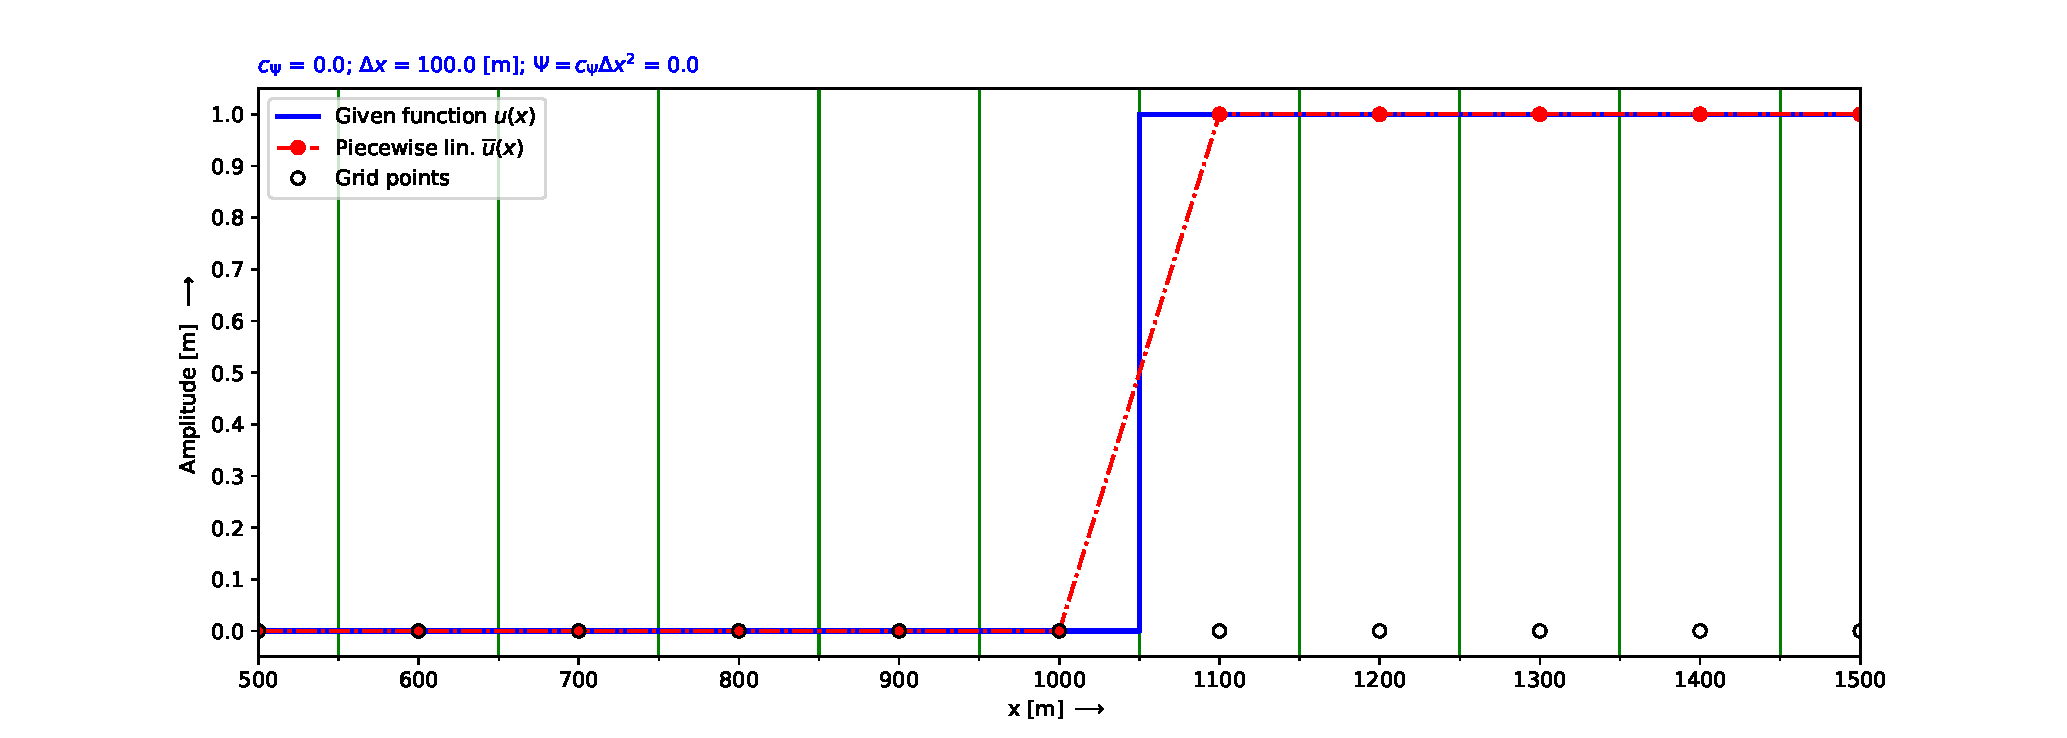
\includegraphics[width=1.0\textwidth]{figures/regul_2_1d_step_function_dx100.0_cpsi1e-06.pdf}
        \caption{Step at boundary finite volume, $x = 550\ [m]$}\label{fig:ex_step_function_no_regularization_b}
    \end{subfigure}
    \caption{Step function approximated by a piecewise linear function (red line with dots at the nodes), $c_{\Psi} = 0$, $\Dx = 100\ [m]$ and $\Psi = 0$. The thin green vertical lines indicate the  borders of the finite volumes. \label{fig:ex_step_function_no_regularization}}
\end{figure}
As seen from  \autoref{fig:ex_step_function_no_regularization} the step is more taken into account as is presented in \autoref{fig:straight_forward_discretization}.
Which looks quite well, but what are the values of the second derivative of the solution.
For $\Dx=\SI{100}{[\metre]}$ the absolute value of the second derivative is $0.5/(100)^2$ (\autoref{fig:ex_step_function_no_regularization_a}) and $1.0/(100)^2$ (\autoref{fig:ex_step_function_no_regularization_b}).


There are two options to estimate this step function by a piecewise linear smooth function with the same numerical accuracy:
\begin{enumerate}
    \item Regularization with using a large grid size, the numerical solution is less close to the step function (see \autoref{fig:ex_step_function_larger_dx})
    \item Regularization with using a small grid size, the numerical solution is closer to the step function (see \autoref{fig:ex_step_function_smaller_dx}),
\end{enumerate}
Both options has the same value for $c_{\Psi} = 4$. Meaning that the step is represented by the same number of grid cells.
How to estimate $c_\Psi$ can be read in \autoref{sec:error_estimation}.
It is up to the user which regularization is can be used for the numerical simulation.
A better representation of the step function need a smaller grid size.
\begin{figure}[H]
    \centering
    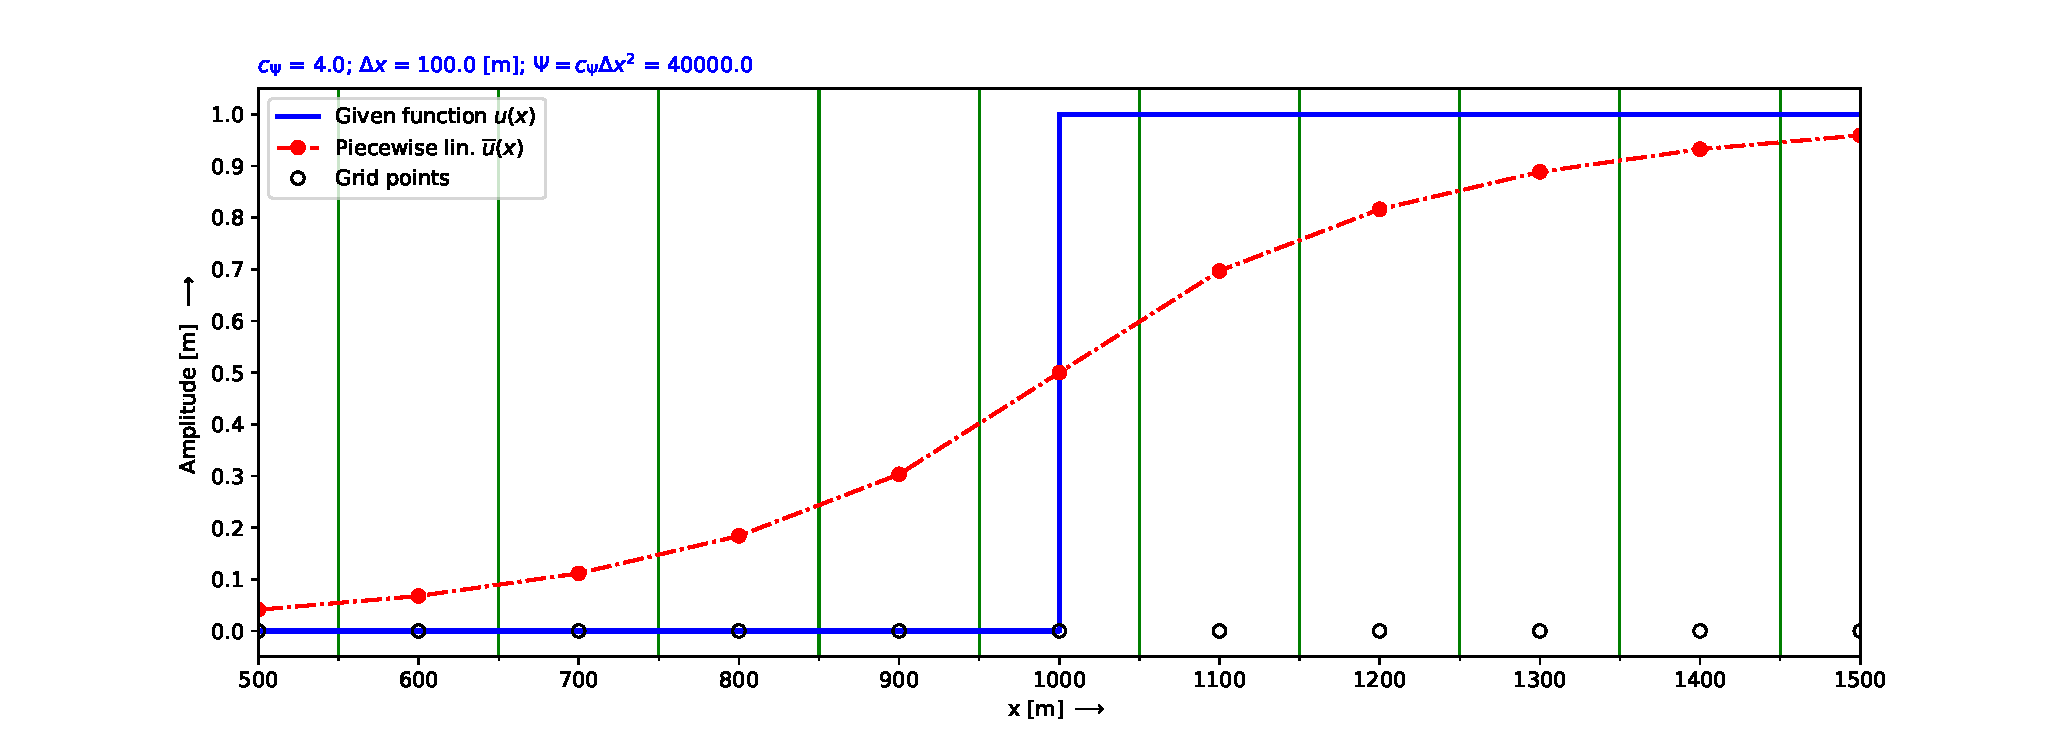
\includegraphics[width=1.0\textwidth]{figures/regul_1d_step_function_dx100.0_cpsi4.0.pdf}
    \caption{Step function approximated by a piecewise linear function (red line with dots at the nodes), $c_{\Psi} = 4$, $\Dx = 100\ [m]$ and $\Psi = 40000$. The thin green vertical lines indicate the  borders of the finite volumes. \label{fig:ex_step_function_larger_dx}}
\end{figure}
\begin{figure}[H]
    \centering
    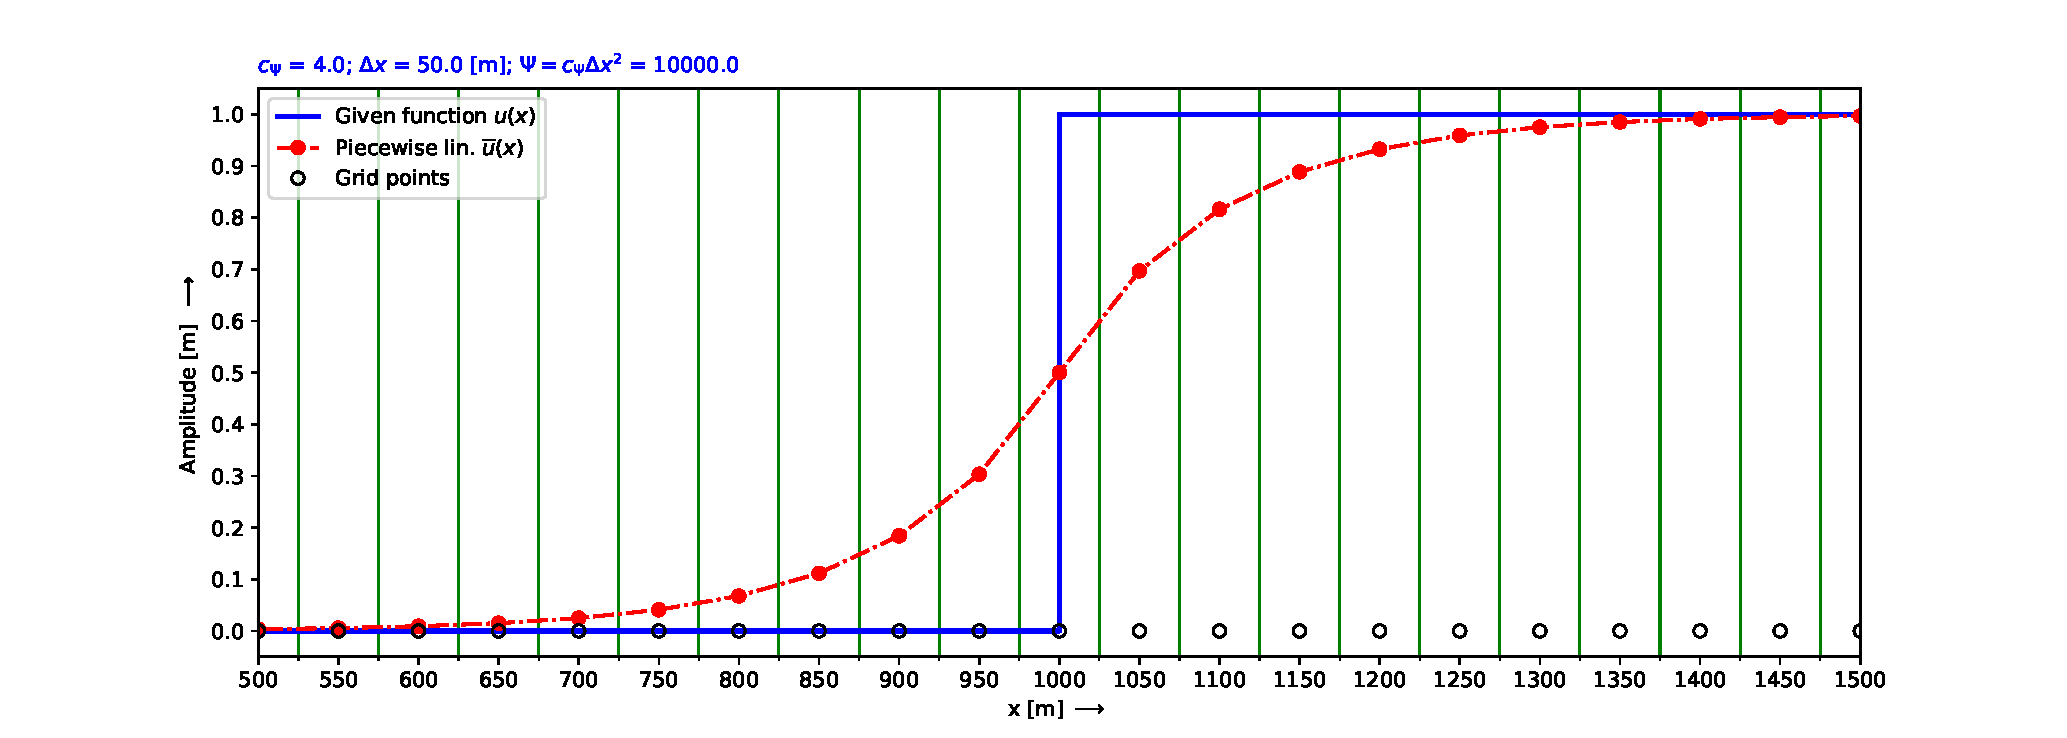
\includegraphics[width=1.0\textwidth]{figures/regul_1d_step_function_dx50.0_cpsi4.0.pdf}
    \caption{Step function approximated by a piecewise linear function (red line with dots at the nodes), $c_{\Psi} = 4$, $\Dx = 50\ [m]$ and $\Psi =10000$. he thin green vertical lines indicate the  borders of the finite volumes. \label{fig:ex_step_function_smaller_dx}}
\end{figure}
\vspace*{0.5\baselineskip}
%
%--------------------------------------------------------------------------------
\subsection{Small and a large gradient in the data set}
To show the influence of  regularization a more general data set is chosen, \citet{Borsboom1998} (given function, here adjusted).
A given function  with a small (smooth) and large  (steep) gradients in the data set is chosen.
The function is defined by:
\begin{align}
u_{given}(x) =
\begin{cases}
    10 \left(\half - \half \tanh{(20x/1000-6)}\right), & \text{if} \quad 0\ [m] \leq x \leq 650\ [m],
    \\
    10, & \text{if} \quad 650\ [m] < x \geq 1000 \ [m],
\end{cases}
\end{align}
and shown in \autoref{fig:tanh_step}:
\begin{figure}[H]
    \centering
    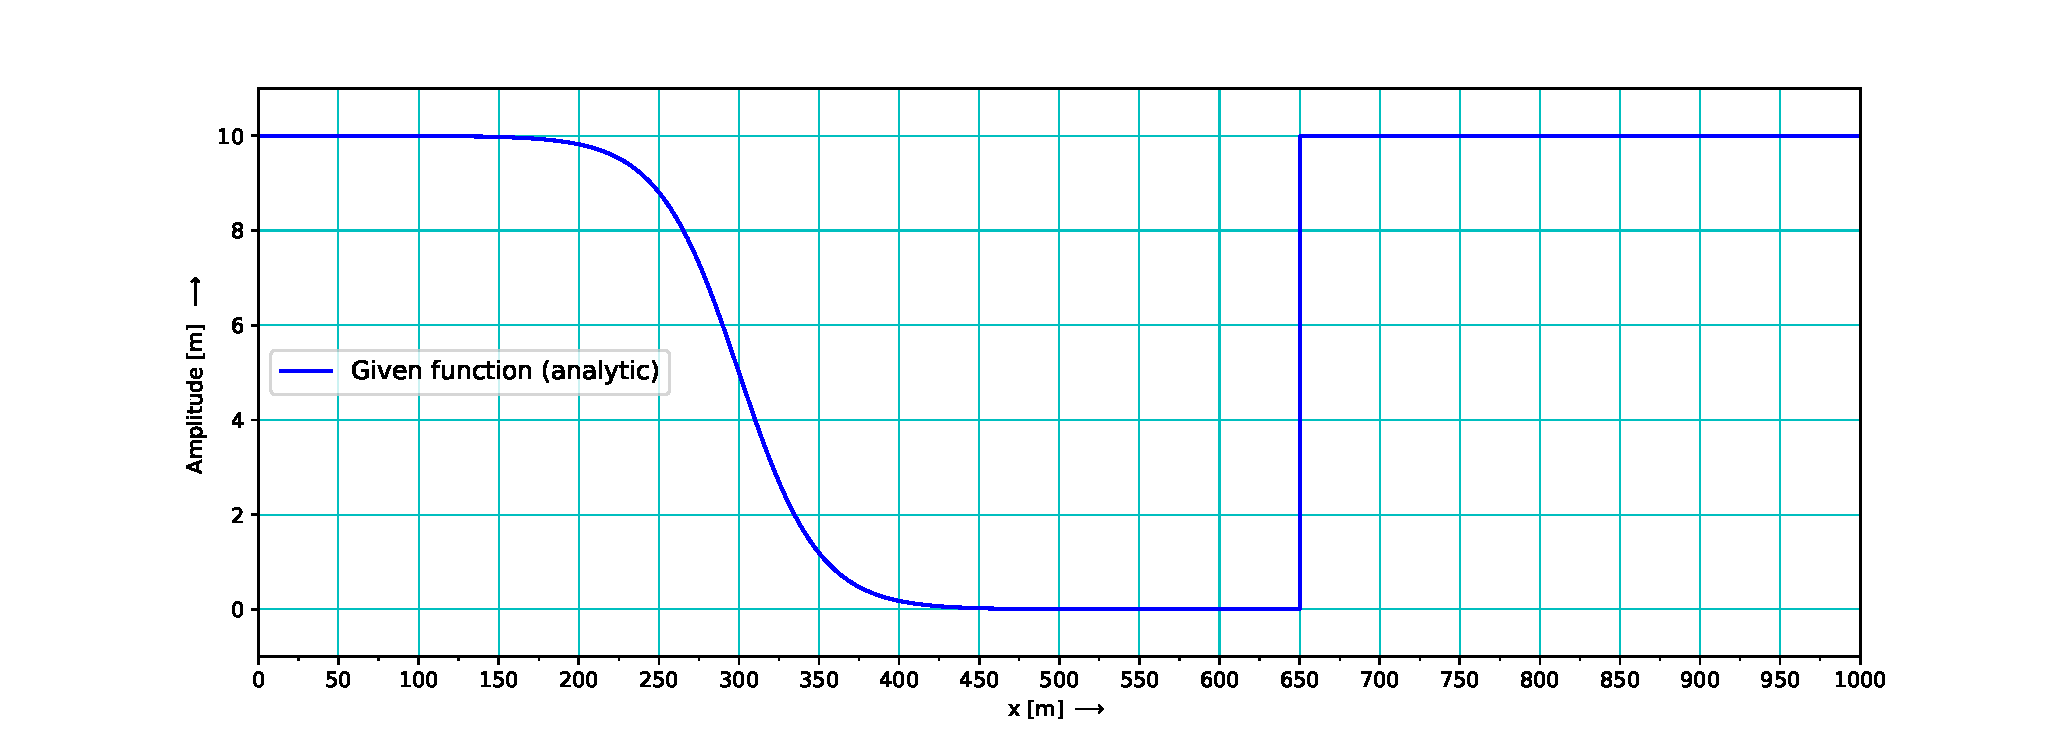
\includegraphics[width=1.0\textwidth]{figures/regul_tanh_step.pdf}
    \caption{Large and small gradients in given function. \label{fig:tanh_step}}
\end{figure}

First guess of regularization:
\begin{figure}[H]
    \centering
    \begin{subfigure}[t]{0.49\textwidth}
    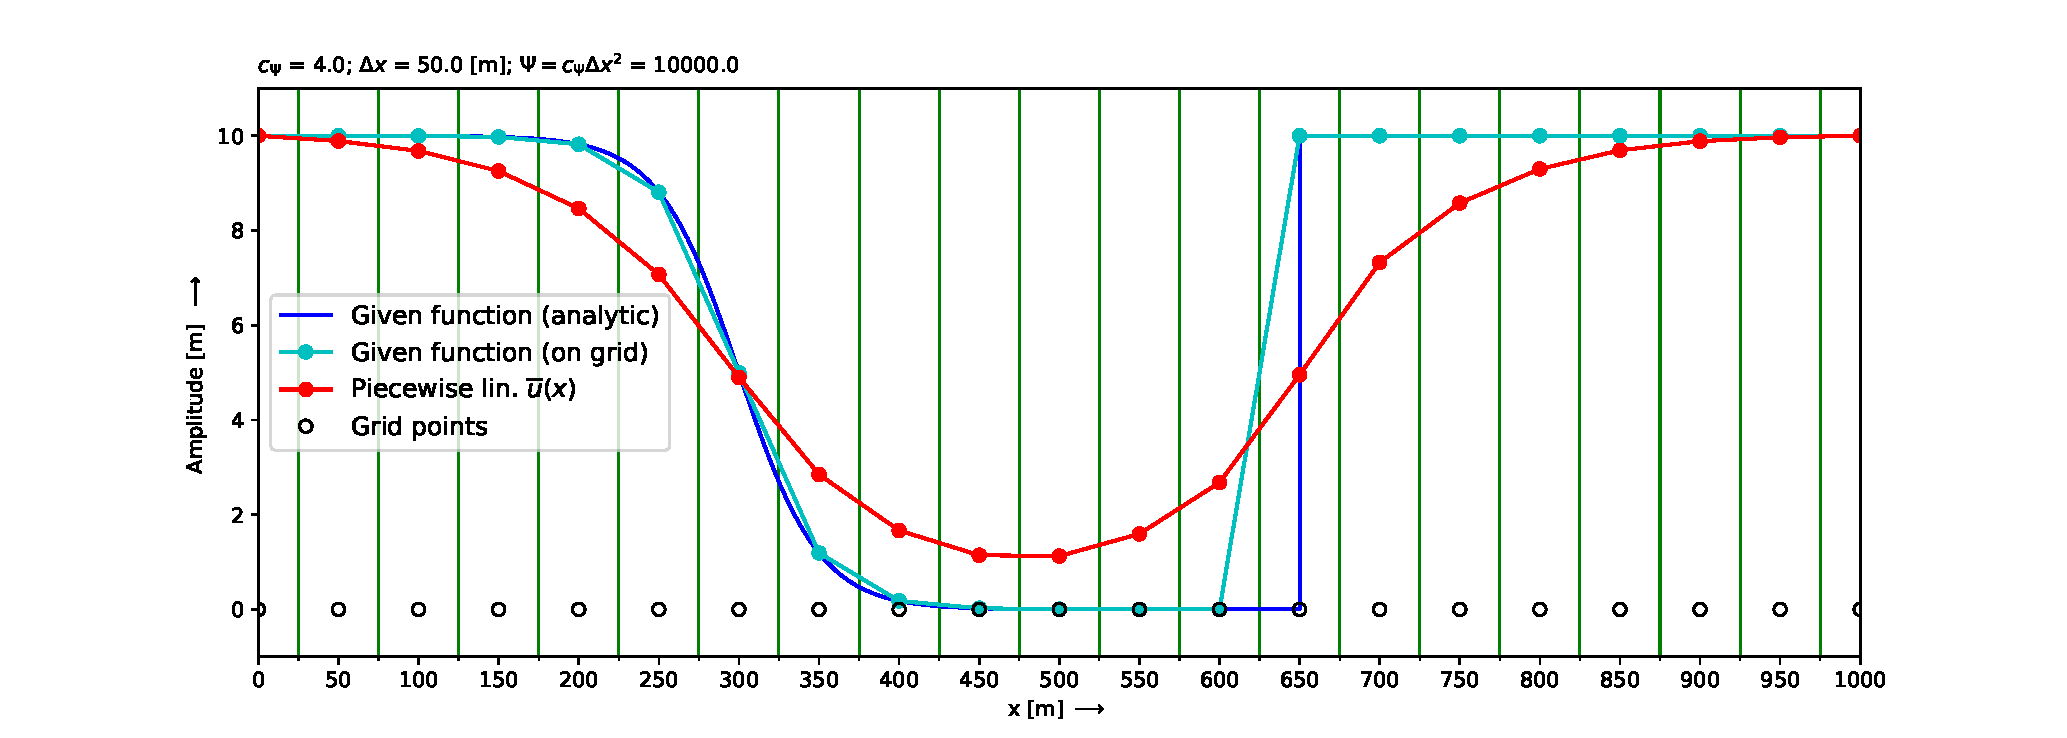
\includegraphics[width=1.0\textwidth]{figures/regul_1_1d_scalar_dx50.0_cpsi4.0.pdf}
\caption{Grid size $\Dx = 50\ [m]$}
    \end{subfigure}
    \hfill
    \begin{subfigure}[t]{0.49\textwidth}
        \centering
        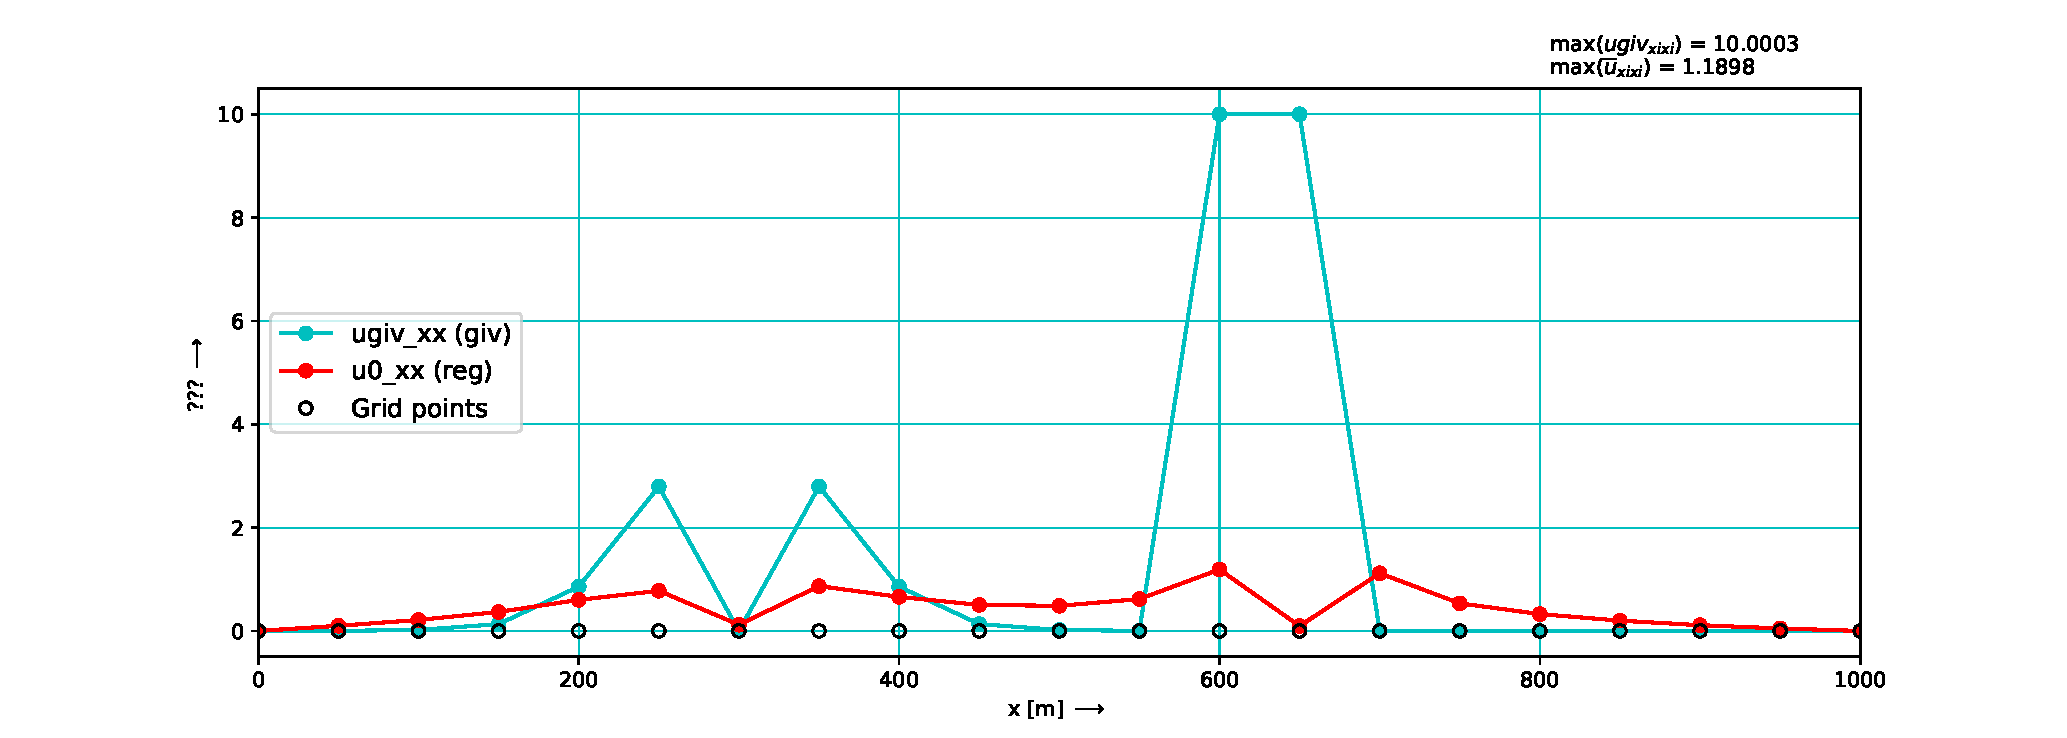
\includegraphics[width=1.0\textwidth]{figures/regul_2_1d_scalar_dx50.0_cpsi4.0.pdf}
        \caption{Second derivatives, normalized grid size $\Dxi = 1$.}
    \end{subfigure}
    \caption{Initial guess ($c_\Psi = 4, \Dx = 50\ [m]$)}
\end{figure}

There are two options to adjust the data:
\begin{enumerate}
    \item increase the regularization coefficient or
    \item choose a smaller grid size.
\end{enumerate}
%--------------------------------------------------------------------------------
\paragraph*{Regularization coefficient increased}
Increasing the regularization coefficient $c_\Psi$:
\begin{figure}[H]
    \centering
    \begin{subfigure}[t]{0.49\textwidth}
        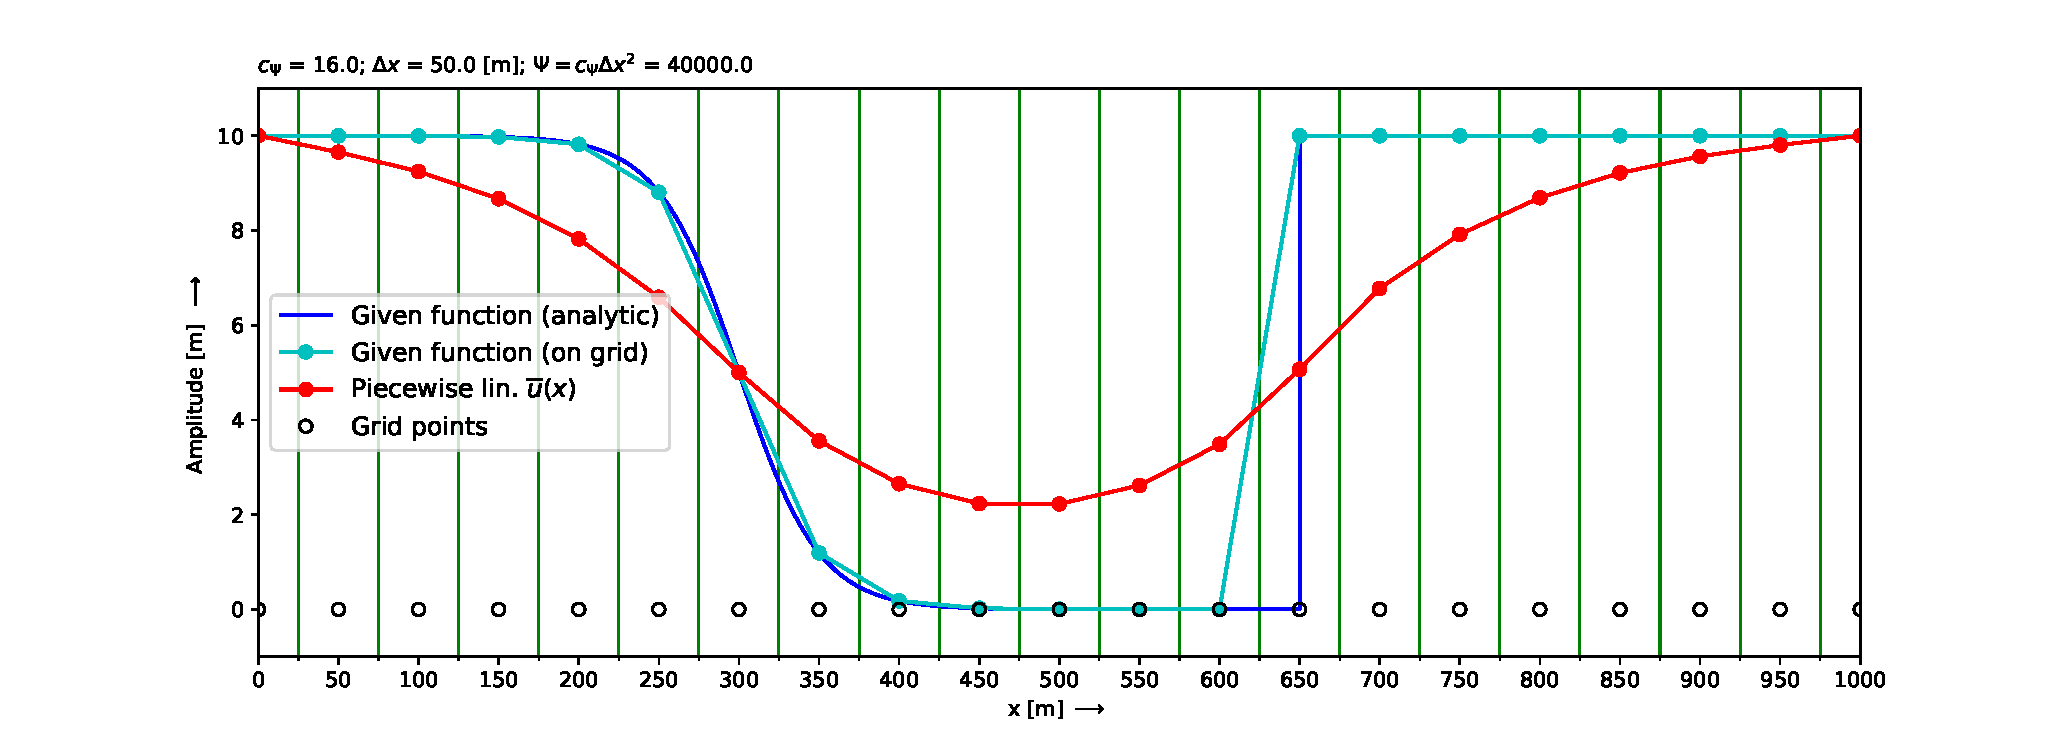
\includegraphics[width=1.0\textwidth]{figures/regul_1_1d_scalar_dx50.0_cpsi16.0.pdf}
        \caption{Grid size $\Dx = 50\ [m]$}
    \end{subfigure}
    \hfill
    \begin{subfigure}[t]{0.49\textwidth}
        \centering
        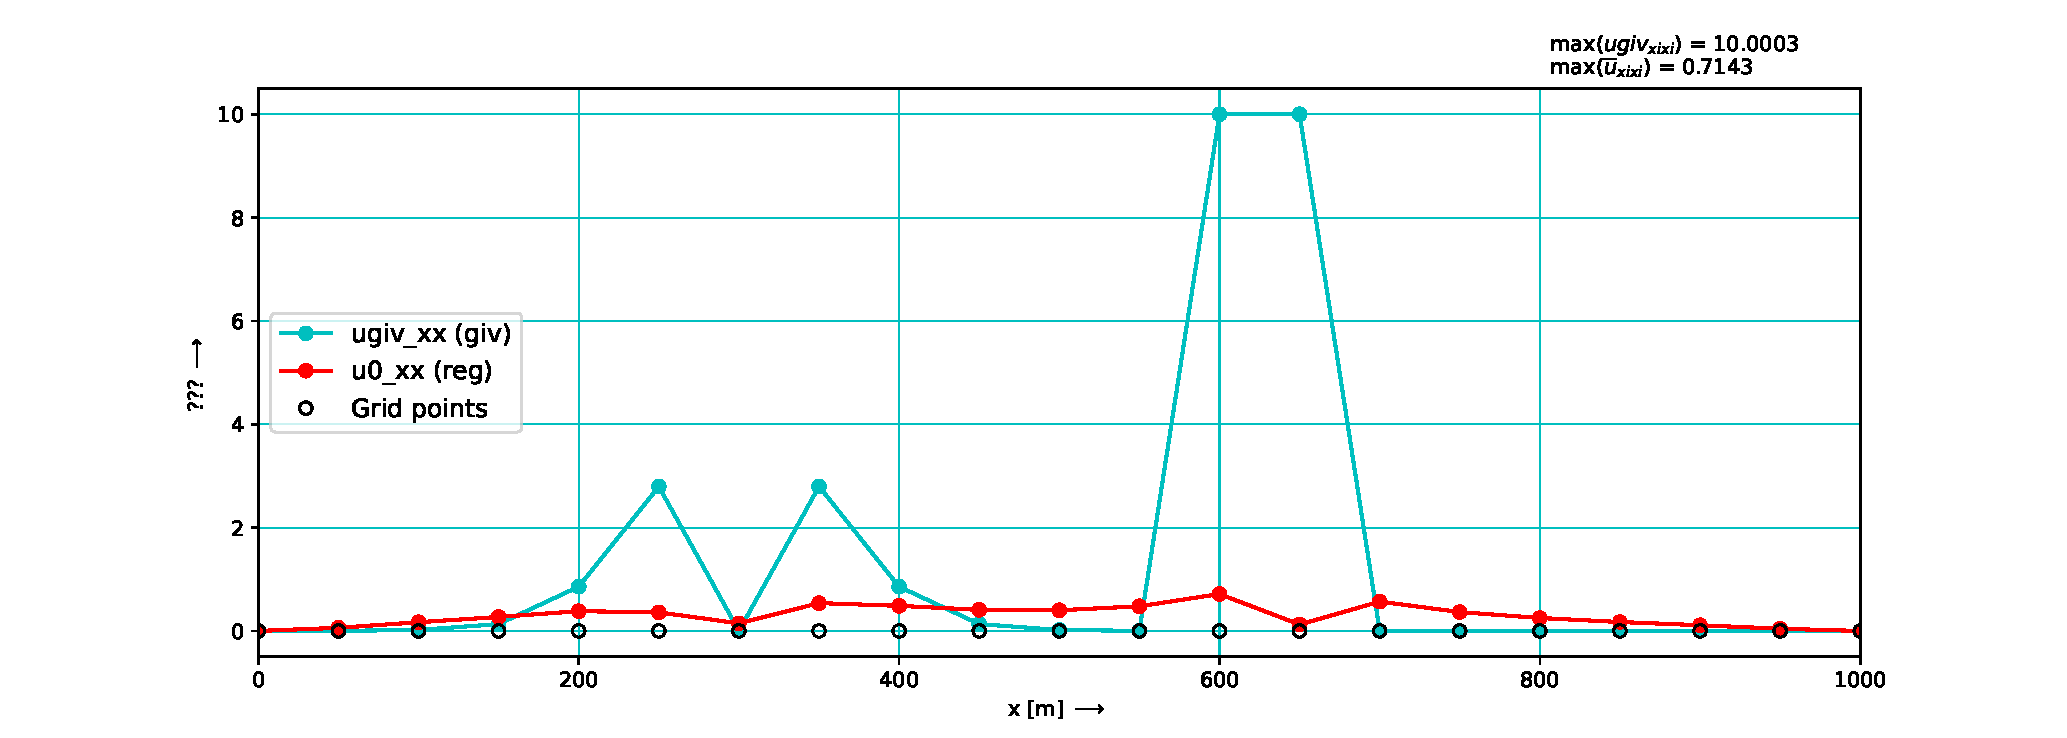
\includegraphics[width=1.0\textwidth]{figures/regul_2_1d_scalar_dx50.0_cpsi16.0.pdf}
        \caption{Second derivatives, normalized grid size $\Dxi = 1$.}
    \end{subfigure}
    \caption{Regularization coefficient increased to 16 ($c_\Psi = 16, \Dx = 50\ [m]$)}
\end{figure}
%--------------------------------------------------------------------------------
\paragraph*{Grid size decreased}
Decrease the grid size $\Dx$:
\begin{figure}[H]
    \centering
    \begin{subfigure}[t]{0.49\textwidth}
        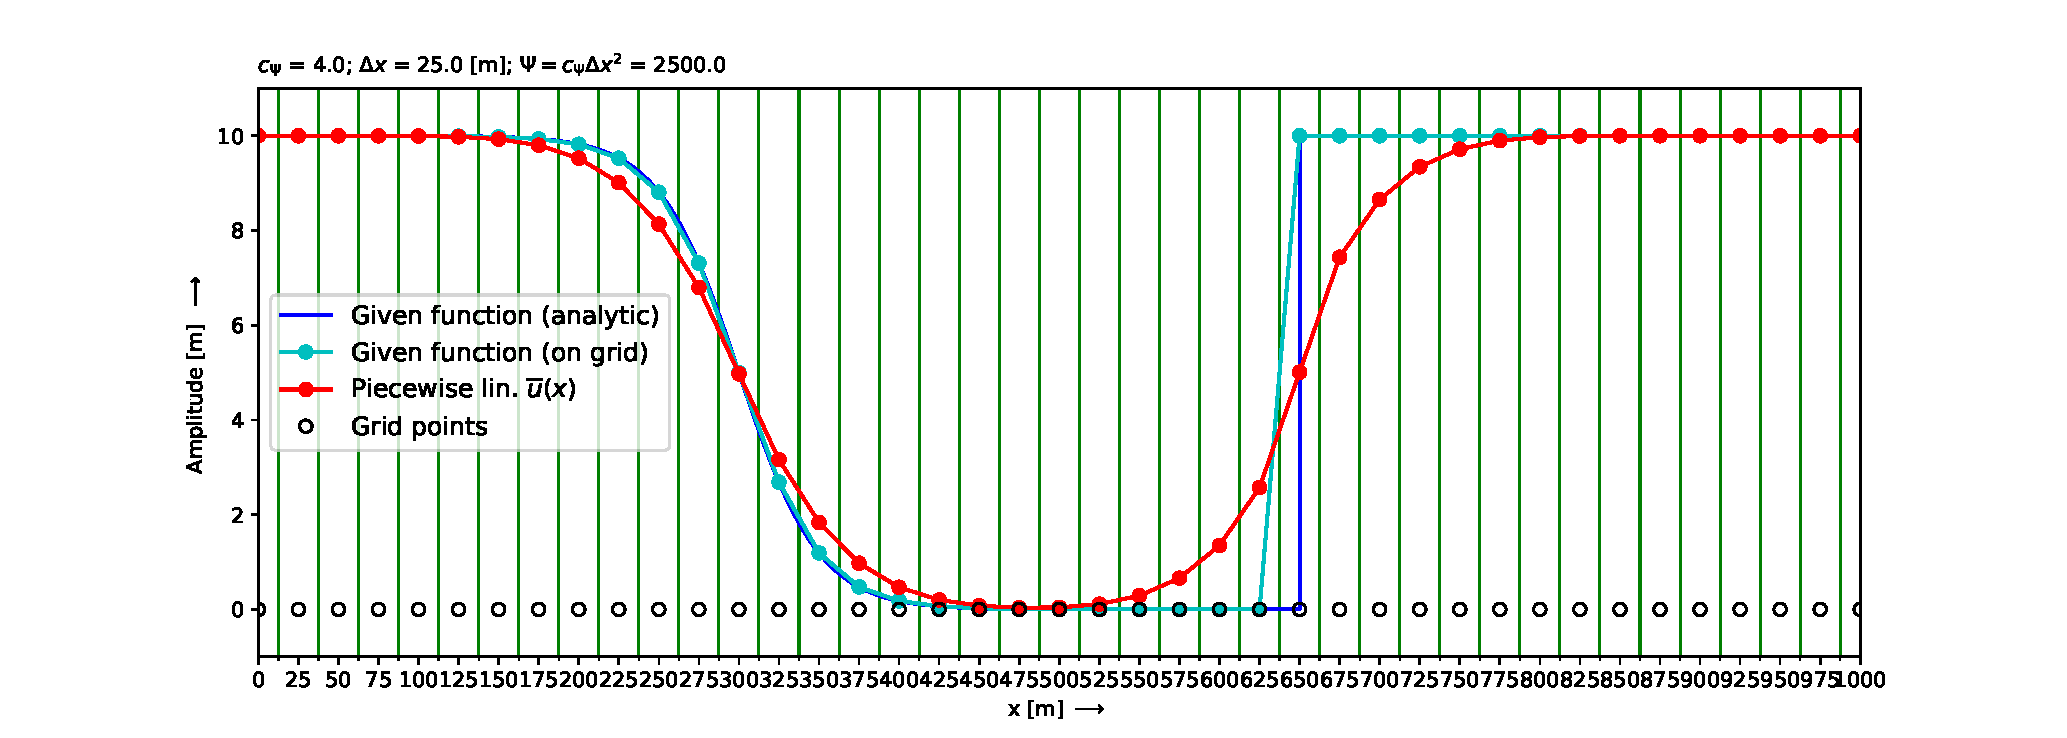
\includegraphics[width=1.0\textwidth]{figures/regul_1_1d_scalar_dx25.0_cpsi4.0.pdf}
        \caption{Step at grid node, $c_\Psi = 4, \Dx = 25\ [m]$}
    \end{subfigure}
    \hfill
    \begin{subfigure}[t]{0.49\textwidth}
        \centering
        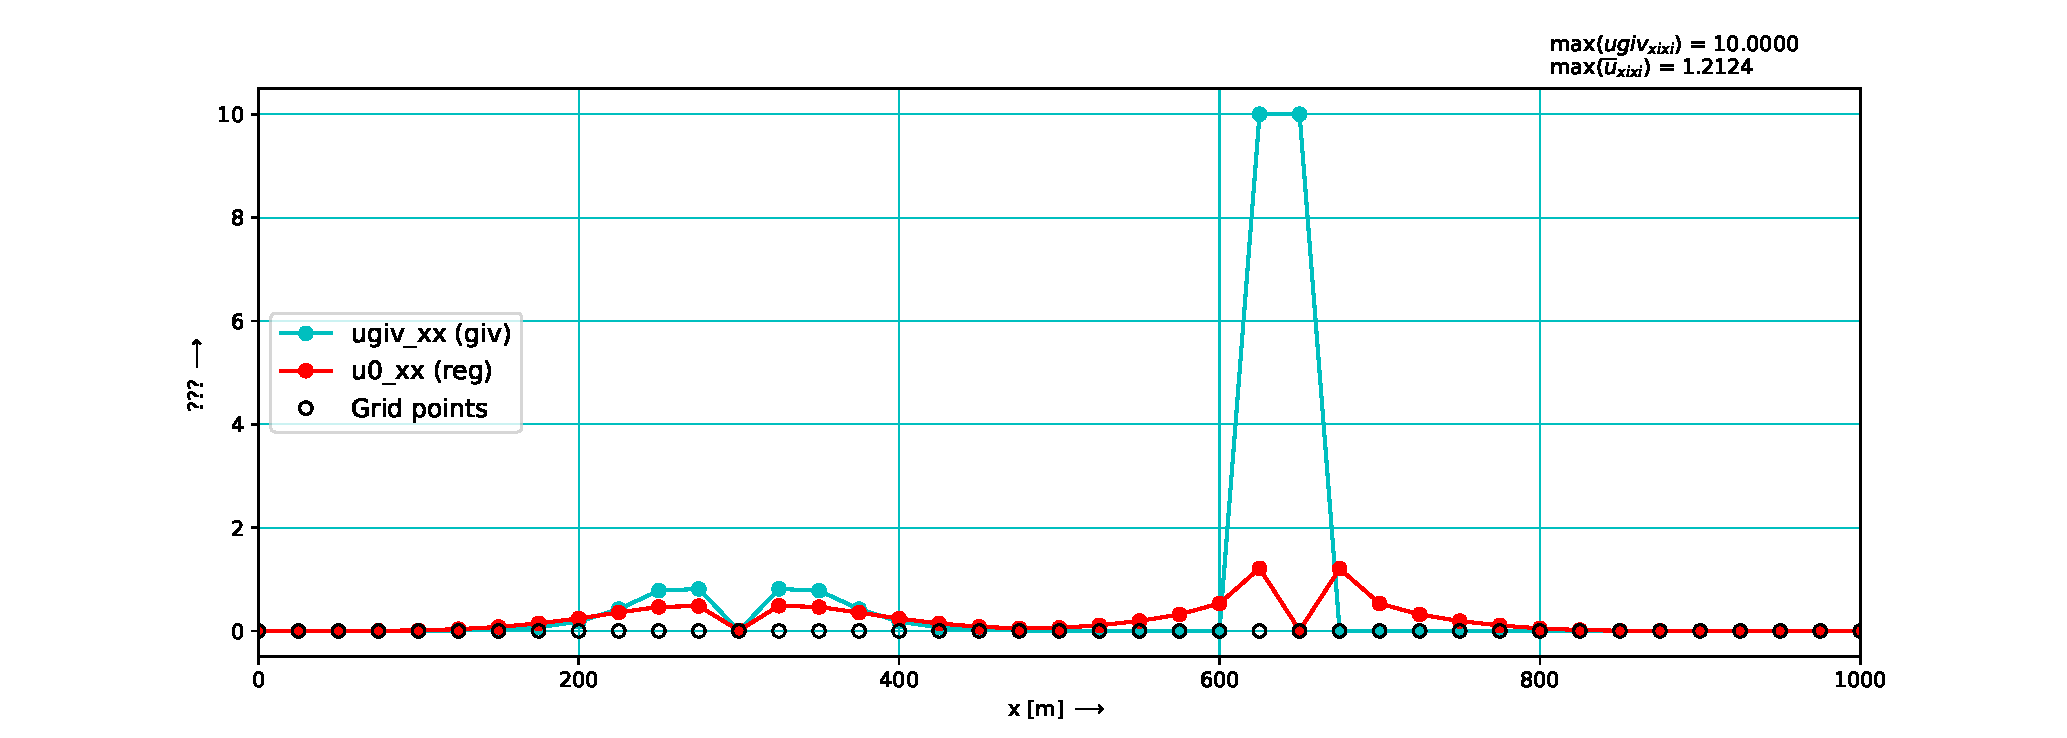
\includegraphics[width=1.0\textwidth]{figures/regul_2_1d_scalar_dx25.0_cpsi4.0.pdf}
        \caption{Second derivatives.}
    \end{subfigure}
    \caption{Grid size decreased to $25\ [m]$ ($c_\Psi = 4, \Dx = 25\ [m]$)}
\end{figure}
%------------------------------------------------------------------------------
\section{Compatible initialization}
To assure that the given initial condition(s) are compatible with the numerical scheme, the given function need to fulfill the follow equation:
\begin{align}
    \int_{x_{i-\half}}^{x_{i+\half}} \overline u_{initial}\, dx = \int_{x_{i-\half}}^{x_{i+\half}} u_{given}\, dx \label{eq:compatible_initialization}
\end{align}
where $\overline{u}$ is the piecewise function and $u_{given}$ the given initial condition.
In case the function $u_{given}$ is an integrable analytic function the integral can be exact computed.
In discrete form the equation for each control volume reads:
\begin{align}
    \frac{\Dx_{i-\half}}{2}\,\frac{u_{i-1} + 3 u_i}{4} +
    \frac{\Dx_{i+\half}}{2}\,\frac{3 u_i + u_{i+1}}{4} = \int_{x_{i-\half}}^{x_{i+\half}} u_{given}\, dx
\end{align}
Extra equations are needed for the boundary conditions, the following boundary treatment is used at $x=2$ (see  \autoref{sec:boundary_conditions}):
\begin{align}
    \frac{1}{12} u_0 + \frac{10}{12}u_1 + \frac{1}{12} u_2 = u_{given}(2)
\end{align}
and similar at the other boundary ($x=10$).
An illustration off the result of \autoref{eq:compatible_initialization} is given in \autoref{fig:compatible_initial_condition}.
\begin{figure}[H]
    \centering
    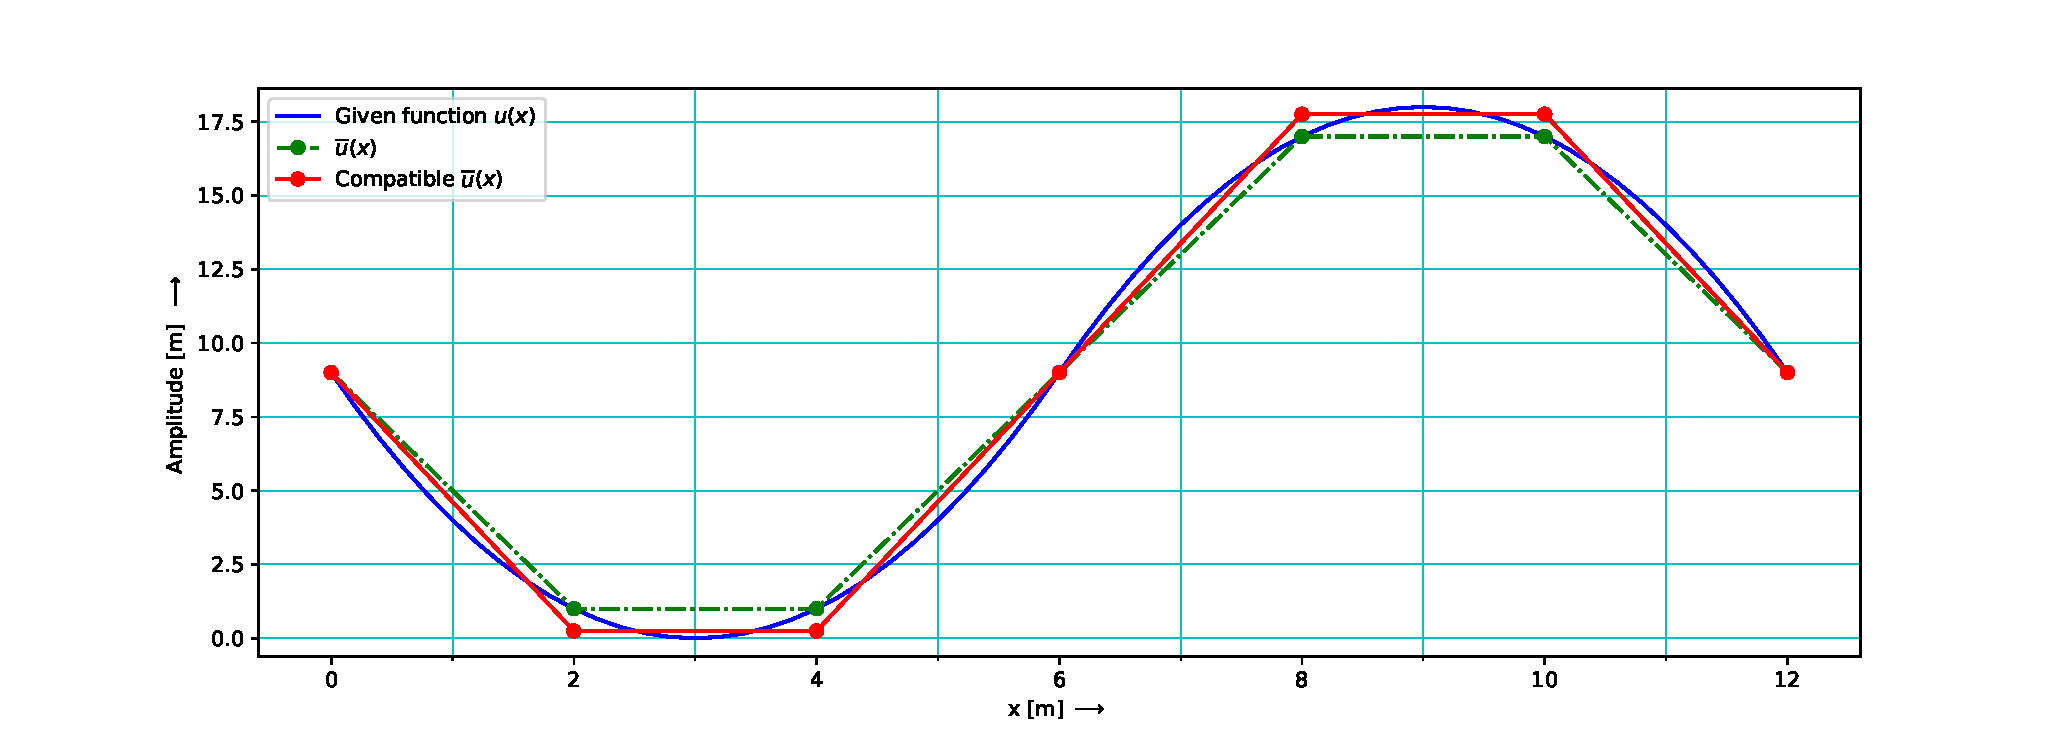
\includegraphics[width=0.9\textwidth]{figures/compatible_initialization_lx=12.0_dx=2.0.pdf}
    \caption[Illustration of compatible quadratic function]{Illustration of compatible quadratic function. Given function in blue. Compatible function in red. In green lines through nodes lying on the given function. Control volumes in between the green vertical lines. And the gray areas are virtual and are not belonging to the water body (see \autoref{fig:water_body_fve_bc_at_node}). The integral over the control volume of the the given function is better represented by the red-function then by the green-function. }\label{fig:compatible_initial_condition}
    % python script: compatible_initial_function.py
\end{figure}
Some numerical items used to generate \autoref{fig:compatible_initial_condition} are $x \in [0, 12]$, $\Dx=2$ and the given function reads:
\begin{align}
    &u_{given}(x) =
    \begin{cases}
        (x-3)^2 & \qquad x < 6
        \\ 
        -(x-3)^2 + 18 & \qquad x \geq 6
    \end{cases}
\end{align}
%------------------------------------------------------------------------------
%\part{1D Wave}
%%------------------------------------------------------------------------------
\chapter{Towards the shallow water equations}\label{sec:1d_swe}
Consider the non-linear wave equation when the pressure gradient is explicitly expressed as the gradient of the water level ($\zeta$):
\begin{subequations}
    \begin{align}
        &\underbrace{\pdiff{h}{t}}_{\textsl{Time derivative}}  +
        \underbrace{\pdiff{q}{x}}_{\textsl{Mass flux}} =0,
        \\
        &\underbrace{\pdiff{q}{t}}_{\textsl{Time derivative}}  +
        \underbrace{\pdiff{q^2/h}{x}}_{\textsl{Convection}} +
        \underbrace{gh \pdiff{\zeta}{x}}_{\textsl{Pressure gradient}} +
        \nonumber \\*
        & \qquad \qquad +
        \underbrace{c_f\frac{q\abs{q}}{h^2}}_{\textsl{Bed shear stress}}
        -\underbrace{\pdiff{}{x}\left( \nu h \pdiff{q/h}{x}\right)}_{\textsl{Viscosity}} = 0,
        \\
        &\zeta = h + z_b
    \end{align}
    \label{eq:1d_non_linear_wave2}
\end{subequations}
%
with
\begin{symbollist}
    \item[$h$] Total water depth ($h = \zeta - z_b$), \bunit{\metre}.
    \item[$z_b$] Bed level w.r.t.\ reference plane, positive upward, \bunit{\metre}.
    \item[$q$] Flow ($q = hu$), \bunit{\square\metre\per\second}.
    \item[$\zeta$] Water level w.r.t.\ reference plane ($\zeta = h + z_b$), positive upward, \bunit{\metre}.
    \item[$u$] Velocity ($u = q/h$), \bunit{\metre\per\second}.
    \item[$g$] Acceleration due to gravity, \bunit{\metre\per\square\second}.
    \item[$\nu$] Kinematic viscosity, \bunit{\square\metre\per\second}.
\end{symbollist}
\vspace{1cm}
\begin{figure}[H]
    \centering
    \begin{center}
        \def\svgwidth{1.0\textwidth} % scaling text
        \resizebox{0.9\textwidth}{!}{
            \input{figures/definition_variables.pdf_tex}
        }
    \end{center}
    \caption{Definition sketch of water level ($\zeta$), bed level ($z_b$) and total water depth ($h$)}\label{fig:definition_variables_1d}
\end{figure}
If $u$ is needed for other processes (like morphology and/or post processing) it can be computed according the next equation:
\begin{align}
    u & = \frac{q}{h}.
\end{align}
In the finite volume approach these equations read:
\begin{subequations}
    \begin{align}
        \int_\Omega \pdiff{h}{t}\, d\omega & +\int_\Omega \pdiff{q}{x}\, d\omega=0,
        \\
        \int_\Omega \pdiff{q}{t}\, d\omega & + \int_\Omega \pdiff{q^2/h}{x}\, d\omega + \int_\Omega gh \pdiff{\zeta}{x}\, d\omega  +
        \nonumber \\*
        & \qquad \qquad + \int_{\Omega} c_f\frac{q\abs{q}}{h^2} \, d\omega - \int_{\Omega} \pdiff{}{x}\left( \nu h \pdiff{q/h}{x}\right) \, d\omega= 0,
        \\
        \int_\Omega \zeta\, d\omega & = \int_\Omega h\, d\omega + \int_\Omega z_b\, d\omega
    \end{align}
\end{subequations}

In this document we will end up with an implementation description of the 1D shallow water equation.
We start a zero-dimensional implementation of a source term, representing the source and sink of external influences, like a power plant.
Here we will show the results of a Brusselator \citep{AultHolmgreen2003} and of a air pollution model \citep[ex.\ 1.1 pg.\ 7]{HundsdorferAndVerwer2003}.
Then we continue with the one dimensional advection/transport equation than a one dimensional wave equation without convection, then with convection and at last with a bottom friction term.
in this sequence we are missing the viscosity term, that term will be investigated by the advection-diffusion equation.

Because we will handle the shallow water equations in the variables $h$ and  $q$ and not in $\zeta$ and $u$ the equations does have always a non-linear behaviour, only for very small amplitude the behaviour is like a linear system.
For linear wave equations the behaviour is always linear, even for large amplitudes, which is not the case for the equations we consider.
%------------------------------------------------------------------------------
\section{0-D Source/sink term }\label{sec:0d_source_and_sink}
In this section a zero-dimensional model is implementation of the source term, representing the source and sink of external influences, like a power plant.
The main (simple) equation will look like:
\begin{align}
    \pdiff{\vec{u}}{t} = \vec{f}(\vec{u},t)
\end{align}
Here we will show the mathematical and implementation of an air pollution model, \autoref{sec:air_pollution} \citep[ex.\ 1.1 pg.\ 7]{HundsdorferAndVerwer2003} and a Brusselator, \autoref{sec:brusselator}  \citep{AultHolmgreen2003}.
Some results are shown in \autoref{sec:0d_numerical_experiments}.
%------------------------------------------------------------------------------
\subsection{Air pollution}\label{sec:air_pollution}
%------------------------------------------------------------------------------
\paragraph*{Analytic description}
We illustrate the mass action law by the following three reactions between oxygen $O_2$, atomic oxygen $O$, nitrogen oxide $NO$, and nitrogen dioxide $NO_2$ \citep[eq.\ 1.1, page 7]{HundsdorferAndVerwer2003}:
\begin{align}
    NO_2 + h\nu & \xrightarrow{k_1} NO + O, \\
    O + O_2 & \xrightarrow{k_2} O_3, \\
    NO + O_3 & \xrightarrow{k_3} O_2 + NO_2.
\end{align}
These reactions are basic to any tropospheric air pollution model.
The firstreaction is photochemical and says that $NO$ and $O$ are formed from $N02$ by
photo-dissociation caused by solar radiation, indicated by $h\nu$.
This depends on the time of the day and therefore $k_l = k_l(t)$.
We consider the concentrations $u_1 = \bunit{O}$, $u_2 = \bunit{NO}$, $u_3 = \bunit{NO2}$, $u_4 = \bunit{O3}$. The oxygen concentration $\bunit{O_2}$ is treated as constant, and we assume there is a constant source term $\sigma_2$ simulating emission of nitrogen oxide.
The rate functions and stoichiometric matrix are
\begin{align}
    g(t,u) =
    \begin{pmatrix}
        k_1(t) u_3 \\
        k_2u_1 \\
        k_3u_2u_4
    \end{pmatrix}
    ,
    \qquad
    S =
\begin{pmatrix}
    1 & -1 & 0 \\
    1 & 0 & -1 \\
    -1 & 0 & 1 \\
    0 & 1 & -1
\end{pmatrix}
\end{align}
The corresponding ODE system reads:
\begin{align}
    \pdiff{u_1}{t} & = k_1 u_3 -k_2 u_1
    \\
    \pdiff{u_2}{t} & = k_1 u_3 - k_3 u_2 u_4 +\sigma_2
    \\
    \pdiff{u_3}{t} & = k_3 u_2 u_4 - k_1 u_3
    \\
    \pdiff{u_4}{t} & = k_2 u_1 - k_3 u_2 u_4
\end{align}
We see that
\begin{align}
\pdiff{u_1}{t} + \pdiff{u_3}{t} + \pdiff{u_4}{t} = 0,
\end{align}
and
\begin{align}
\pdiff{u_2}{t} + \pdiff{u_3}{t} = \sigma_2 t
\end{align}
hence $\bunit{O} + \bunit{NO2} + \bunit{O3}$ is a conserved quantity while $\bunit{NO} + \bunit{NO2}$ growths
with $\sigma_2t$.
By considering the null-space of $S^T$ it is seen that these are the two
mass laws for this chemical model.

With $\vec{u}(0) = (0.0, \num{2.0e-1}, \num{2.0e-3}, \num{2.0e-1})^T$ and $\sigma_2 = \num{e-7}$, and the coefficients $k$ are defined as (this given conditions are different from the conditions as defined in \citet[pg.\ 8]{HundsdorferAndVerwer2003}:
\begin{align}
    k_1 & = \begin{cases}
        10^{-5} \exp{(7\ {\it g}(t))}
        \\
        \num{e-40}, \qquad \text{during  night}
    \end{cases}
    \\
    k_2 & = \num{2.0e-2}
    \\
    k_3 & = \num{1.0e-3}
\end{align}
with
\begin{align}
    {\it g}(t) =\left(\sin\left(\frac{\pi}{16} (t_h - 4)\right)\right)^{0.2}, \qquad t_h = \frac{t}{3600};
\end{align}
where $t_h$ is the time in hours.
How these equations are discretized is given in \autoref{sec:air_pollution_discretization}.
%
%-------------------------------------------------------------------------------
\paragraph*{Numerical discretization}\label{sec:air_pollution_discretization}
The discretization in $\Delta$-formulation reads:
\begin{align}
    \frac{1}{\Dt}\Delta u_1^{n+1, p+1} & = - \frac{1}{\Dt}(u_1^{n+1,p} - u_1^n) + k_1 (u_3^{n+\theta,p+1}) - k_2 (u_1^{n+\theta,p+1})
    \\
    \frac{1}{\Dt}\Delta u_2^{n+1, p+1} & = - \frac{1}{\Dt}(u_2^{n+1,p} - u_2^n) + k_1(u_3^{n+\theta,p+1}) - k_3 (u_2^{n+\theta,p+1}) (u_4^{n+\theta,p+1}) +\sigma_2
    \\
    \frac{1}{\Dt}\Delta u_3^{n+1, p+1} & = - \frac{1}{\Dt}(u_3^{n+1,p} - u_3^n) + k_3 (u_2^{n+\theta,p+1}) (u_4^{n+\theta,p+1}) - k_1(u_3^{n+\theta,p+1})
    \\
    \frac{1}{\Dt}\Delta u_4^{n+1, p+1} & = - \frac{1}{\Dt}(u_4^{n+1,p} - u_4^n) + k_2(u_1^{n+\theta,p+1}) - k_3 (u_2^{n+\theta,p+1}) (u_4^{n+\theta,p+1})
\end{align}
with linearization of $\vec{u}^{n+\theta,p+1}$ yields:
\begin{align}
    \frac{1}{\Dt}\Delta u_1^{n+1, p+1} & =
    - \frac{1}{\Dt}(u_1^{n+1,p} - u_1^n) +
    \nonumber \\*
    & + k_1 (u_3^{n+\theta,p} + \theta \Delta u_3^{n+1, p+1}) - k_2 (u_1^{n+\theta,p} + \theta \Delta u_1^{n+1, p+1})
    \\
    %-----
    \frac{1}{\Dt}\Delta u_2^{n+1, p+1} & = - \frac{1}{\Dt}(u_2^{n+1,p} - u_2^n) + k_1(u_3^{n+\theta,p} + \theta \Delta u_3^{n+1, p+1}) +
    \nonumber \\*
    & - k_3 (u_2^{n+\theta,p} + \theta \Delta u_2^{n+1, p+1}) (u_4^{n+\theta,p} + \theta \Delta u_4^{n+1, p+1}) +\sigma_2
    \\
    %-----
    \frac{1}{\Dt}\Delta u_3^{n+1, p+1} & = - \frac{1}{\Dt}(u_3^{n+1,p} - u_3^n) + k_3 (u_2^{n+\theta,p} + \theta \Delta u_2^{n+1, p+1}) (u_4^{n+\theta,p} +
    \nonumber \\*
    & +  \theta \Delta u_4^{n+1, p+1}) - k_1(u_3^{n+\theta,p} + \theta \Delta u_3^{n+1, p+1})
    \\
    %-----
    \frac{1}{\Dt}\Delta u_4^{n+1, p+1} & = - \frac{1}{\Dt}(u_4^{n+1,p} - u_4^n) + k_2(u_1^{n+\theta,p} + \theta \Delta u_1^{n+1, p+1}) +
    \nonumber \\*
    & - k_3 (u_2^{n+\theta,p} + \theta \Delta u_2^{n+1, p+1}) (u_4^{n+\theta,p} + \theta \Delta u_4^{n+1, p+1})
\end{align}
and rearrange the system of equations to $\mat{A}\vec{x}=\vec{b}$, yields
\begin{align}
    \frac{1}{\Dt}\Delta u_1^{n+1, p+1} &  - k_1  \theta \Delta u_3^{n+1, p+1} + k_2  \theta \Delta u_1^{n+1, p+1}  =
    \nonumber \\*
    & = - \frac{1}{\Dt}(u_1^{n+1,p} - u_1^n) + k_1 u_3^{n+\theta,p} - k_2 u_1^{n+\theta,p}
    \\
    %-----
    \frac{1}{\Dt}\Delta u_2^{n+1, p+1} & - k_1 \theta \Delta u_3^{n+1, p+1}
    + k_3 \theta u_4^{n+1,p} \Delta u_2^{n+1, p+1} + k_3 \theta u_2^{n+1,p} \Delta u_4^{n+1, p+1}  =
    \nonumber \\*
    & = - \frac{1}{\Dt}(u_2^{n+1,p} - u_2^n) + k_1 u_3^{n+\theta,p} - k_3 u_2^{n+\theta,p} u_4^{n+\theta,p} +\sigma_2
    \\
    %-----
    \frac{1}{\Dt}\Delta u_3^{n+1, p+1} & - k_3 u_2^{n+\theta,p} \theta \Delta u_4^{n+1, p+1} - k_3 u_4^{n+\theta,p} \theta \Delta u_2^{n+1, p+1} + k_1 \theta \Delta u_3^{n+1, p+1}  =
    \nonumber \\*
    & = - \frac{1}{\Dt}(u_3^{n+1,p} - u_3^n) + k_3 u_2^{n+\theta,p} u_4^{n+\theta,p} - k_1 u_3^{n+\theta,p}
    \\
    \frac{1}{\Dt}\Delta u_4^{n+1, p+1}&  - k_2 \theta \Delta u_1^{n+1, p+1}  + k_3 u_2^{n+\theta,p}\theta \Delta u_4^{n+1, p+1} +k_3 u_4^{n+\theta,p} \theta \Delta u_2^{n+1, p+1} =
    \nonumber \\*
    & = - \frac{1}{\Dt}(u_4^{n+1,p} - u_4^n) + k_2 u_1^{n+\theta,p} - k_3 u_2^{n+\theta,p} u_4^{n+\theta,p}
\end{align}
%------------------------------------------------------------------------------
\subsection{Brusselator}\label{sec:brusselator}
%------------------------------------------------------------------------------
\paragraph*{Analytic description}
The  ODE system for the Brusselator reads \citet[eq.\ 14,15]{AultHolmgreen2003}:
\begin{align}
    \pdiff{u_1}{t} & = 1 - (k_2 + 1) u_1 + k_1 u_1^2 u_2,
    \\
    \pdiff{u_2}{t} & = k_2 u_1 - k_1 u_1^2 u_2
    \label{eq:brusselator}
\end{align}
with $k_1 =1$ and  $k_2 = 2.5$ and initial values  $u_1(0)=0$ and $u_2(0) = 0$.
%-------------------------------------------------------------------------------
\paragraph*{Numerical discretization}\label{sec:brusselator_discretization}

The  ODE system for the brusselator reads \citep[eq.\ 14,15]{AultHolmgreen2003}:
\begin{align}
    \pdiff{u_1}{t} & = 1 - (k_2 + 1) u_1 + k_1 u_1^2 u_2,
    \\
    \pdiff{u_2}{t} & = k_2 u_1 - k_1 u_1^2 u_2
\end{align}
The discretization in $\Delta$-formulation reads:
\begin{align}
    \frac{1}{\Dt}\Delta u_1^{n+1, p+1} & = - \frac{1}{\Dt}(u_1^{n+1,p} - u_1^n) + 1 - (k_2 +1) u_1^{n+\theta,p+1} +
    \nonumber \\*
    &  + k_1 \left(u_1^{n+\theta,p+1}\right)^2 u_2^{n+\theta,p+1}
    \\
    \frac{1}{\Dt}\Delta u_2^{n+1, p+1} & = - \frac{1}{\Dt}(u_2^{n+1,p} - u_2^n) + k_2(u_1^{n+\theta,p+1})  +
    \nonumber \\*
    & - k_1 \left(u_1^{n+\theta,p+1}\right)^2 u_2^{n+\theta,p+1}
\end{align}
with linearization of $\vec{u}^{n+\theta,p+1}$ yields:
\begin{align}
    \frac{1}{\Dt}\Delta u_1^{n+1, p+1} & =
    - \frac{1}{\Dt}(u_1^{n+1,p} - u_1^n) + 1 - (k_2 +1) \left(u_1^{n+\theta,p} + \theta \Delta u_1^{n+1, p+1}\right)+
    \nonumber \\*
    &  + k_1 \left(u_1^{n+\theta,p}+\Delta u_1^{n+1, p+1}\right)^2 \left(u_2^{n+\theta,p}+ \Delta u_1^{n+1, p+1}\right)
    \\
    \frac{1}{\Dt}\Delta u_2^{n+1, p+1} & = - \frac{1}{\Dt}(u_2^{n+1,p} - u_2^n) + k_2 (u_1^{n+\theta,p} + \theta \Delta u_1^{n+1, p+1}) +
    \nonumber \\*
    &
    - k_1 \left(u_1^{n+\theta,p}+\Delta u_1^{n+1, p+1}\right)^2 \left(u_2^{n+\theta,p}+ \Delta u_1^{n+1, p+1}\right)
\end{align}
and rearrange the system of equations to $\mat{A}\vec{x}=\vec{b}$ and omitting the second order terms, yields
\begin{align}
    &\frac{1}{\Dt}\Delta u_1^{n+1, p+1}
    - \theta \left(\left(k_2 +1\right) + 2  k_1 u_1^{n+\theta,p} u_2^{n+\theta,p}\right)\Delta u_1 ^{n+1, p+1}
    - \theta k_1 \left(u_1^{n+1, p+1}\right)^2 \Delta u_2 ^{n+1, p+1} =
    \nonumber \\*
    & = - \frac{1}{\Dt}(u_1^{n+1,p} - u_1^n) + 1 - (k_2 +1) u_1^{n+\theta,p} + k_1 \left(u_1^{n+\theta,p}\right)^2 u_2^{n+\theta,p}
    \\
    & \frac{1}{\Dt}\Delta u_2^{n+1, p+1}
    + \theta \left( k_2 + 2 k_1 u_1^{n+\theta,p} u_2^{n+\theta,p} \right) \Delta u_1 ^{n+1, p+1}
    + \theta k_1\left(u_1^{n+1, p+1}\right)^2 \Delta u_2 ^{n+1, p+1}
    = \nonumber \\*
    & =- \frac{1}{\Dt}(u_2^{n+1,p} - u_2^n) + k_2 u_1^{n+\theta,p}
    - k_1 \left(u_1^{n+\theta,p}\right)^2 u_2^{n+\theta,p}
\end{align}
This system can be implemented and solved, some results are presented in \autoref{sec:brusselator}.
%
%------------------------------------------------------------------------------
\section{1-D Advection-diffusion equation}
In this section we will discuss the discretization of an advection-diffusion equation when the constituent does not need to be positive and when the constiuent must be positive.

%------------------------------------------------------------------------------
\subsection{Not strictly positive constituent}\label{sec:1d_adv_diff_equation}
The considered advection-diffusion equation reads:
\begin{align}
    \pdiff{c}{t} + \pdiff{uc}{x} - \pdiff{}{x}\left( \eps \pdiff{c}{x}\right)= 0, \qquad u>0. \label{eq:1d_advection}
\end{align}
A constituent $c$ is transported from the left to the right with the constant  velocity $u\, \bunit{\meter\per\second}$.
Which is discretised on the grid
\begin{figure}[H]
    \centering
    \begin{center}
        \resizebox{0.8\textwidth}{!}{
            \input{figures/water_body_fve_bc_at_node.pdf_tex}
        }
    \end{center}
    \caption[Definition of the grid to solve the 1D-advection equation]{Water body (blue area), finite volumes (green boxes), computational points (open dots), virtual computational points (black dots), boundary points are at $x_{1}$ (inflow/west boundary) and $x_{I+\half}$ (outflow/east boundary).}\label{fig:water_body_fve_bc_at_node_1}
\end{figure}
The finite volume approach for control volume $\Dx_{i+\half}$ of \autoref{eq:1d_advection} reads:
\begin{align}
    \int^{x_{i+\half}}_{x_{i-\half}} \pdiff{c}{t}\, dx
    + \int^{x_{i+\half}}_{x_{i-\half}} \pdiff{uc}{x} \, dx
    - \int^{x_{i+\half}}_{x_{i-\half}} \pdiff{}{x}\left( \eps\pdiff{c}{x} \right)\, dx &= 0
    \\
    \int^{x_{i+\half}}_{x_{i-\half}} \pdiff{c}{t}\, dx + \left. (uc) \right|_{i+\half} -  \left. (uc) \right|_{i-\half}
    -  \left(
    \left. \eps\pdiff{c}{x}\right|_{i+\half} -
    \left. \eps\pdiff{c}{x}\right|_{i-\half}
     \right) & = 0
\end{align}

%------------------------------------------------------------------------------
\paragraph*{Discretization interior}
The discretization in \deltaformulation in the interior of domain $\Omega$ and
for equidistant grid and the mass-matrix as given in \autoref{eq:definition_mass_matrix} reads
\begin{align}
    & \Dx \Dt_{inv} \left(\frac{1}{8} \Delta c^{n+1,p+1}_{i-1} + \frac{6}{8} \Delta c^{n+1,p+1}_{i} + \frac{1}{8} \Delta c^{n+1,p+1}_{i+1}\right)  +
    \nonumber \\*
    &
    + \left\{ \Dx \Dt_{inv} \left( \frac{1}{8}\left( c^{n+1,p}_{i-1} - c^{n}_{i-1} \right) + \frac{6}{8}\left( c^{n+1,p}_{i} - c^{n}_{i} \right) + \frac{1}{8}\left( c^{n+1,p}_{i+1} - c^{n}_{i+1} \right) \right)  \right\} +
    \nonumber \\*
    &\quad  +  u \left( \half (c^{n+\theta, p+1}_{i} + c^{n+\theta,p+1}_{i+1}) -  \half (c^{n+\theta, p+1}_{i-1} +c^{n+\theta,p+1}_{i}) \right) +
    \nonumber \\*
    &\quad - \left( \eps_{i+\half} \frac{c^{n+\theta, p+1}_{i+1} - c^{n+\theta, p+1}_{i}}{\Dx} - \eps_{i-\half} \frac{c^{n+\theta, p+1}_{i} - c^{n+\theta, p+1}_{i-1}}{\Dx}\right) = 0
\end{align}
After linearization of $c^{n+\theta,p+1}$ the discretization reads:
\begin{align}
    \Dx & \Dt_{inv}  \left(\frac{1}{8} \Delta c^{n+1,p+1}_{i-1} + \frac{6}{8} \Delta c^{n+1,p+1}_{i} + \frac{1}{8} \Delta c^{n+1,p+1}_{i+1}\right)
    \nonumber \\*
    & \half \theta u \left(  \Delta c^{n+1,p+1}_{i} + \Delta c^{n+1,p+1}_{i+1} - \left( \Delta c^{n+1,p+1}_{i-1} + \Delta c^{n+1,p+1}_{i}  \right)\right) +
    \nonumber \\*
    & - \theta \frac{\eps_{i+\half}}{\Dx} \Delta c^{n+1, p+1}_{i+1}
    + \theta \left( \frac{\eps_{i+\half}}{\Dx} + \frac{\eps_{i-\half}}{\Dx} \right) \Delta c^{n+1, p+1}_{i} - \theta \frac{\eps_{i-\half}}{\Dx} \Delta c^{n+1, p+1}_{i-1}
    =
    \nonumber \\*
    & = -\left\{ \Dx \Dt_{inv} \left( \frac{1}{8}\left( c^{n+1,p}_{i-1} - c^{n}_{i-1} \right) + \frac{6}{8}\left( c^{n+1,p}_{i} - c^{n}_{i} \right) + \frac{1}{8}\left( c^{n+1,p}_{i+1} - c^{n}_{i+1} \right)\right) + \right.
    \nonumber \\*
    & \qquad + \half u \left((c^{n+\theta, p}_{i} + c^{n+\theta,p}_{i+1}) -  (c^{n+\theta, p}_{i-1} +c^{n+\theta,p}_{i}) \right) +
    \nonumber \\*
    &\qquad - \left. \left( \eps_{i+\half} \frac{c^{n+\theta,p}_{i+1} - c^{n+\theta,p}_{i}}{\Dx} - \eps_{i-\half} \frac{c^{n+\theta,p}_{i} - c^{n+\theta,p}_{i-1}}{\Dx}\right) \right\}
\end{align}

%------------------------------------------------------------------------------
\paragraph*{Discretization at boundaries}
An \textbf{essential} boundary condition at the inflow boundary is needed, left side of the domain.
And, at the right side an outflow boundary 'condition' is required for numerical reasons (called  a \textbf{natural} boundary condition), i.e.\ a discretization of the model equation at the outflow boundary.
The natural boundary conditions is fully determined by the outgoing signal and therefor we use the equation of the outgoing signal, i.e.\ \autoref{eq:left_right_going_equations}.
For the 1-D advection-diffusion equation when omitting the viscosity term it reads:
\begin{align}
    \pdiff{c}{t} + \pdiff{uc}{x}  = 0, \qquad u>0. \label{eq:1d_adv_nat_boundary}
\end{align}

The \textbf{essential} boundary condition at the inflow boundary reads:
\begin{align}
    c(0,t) = c_0(t), \quad t > 0 \qquad \text{(essential boundary)}
\end{align}
The essential boundary condition is supplied at $x_1$ with the following discretization (\autoref{eq:stencil_ess})
\begin{align}
    &\frac{1}{12} \Delta c^{n+1,p+1}_0 + \frac{10}{12} \Delta c^{n+1,p+1}_1 + \frac{1}{12}\Delta c^{n+1,p+1}_2 =
    \nonumber \\*
    &\qquad =c_0(t) - \left( \frac{1}{12} c^{n+1,p}_0 + \frac{10}{12} c^{n+1,p}_1 + \frac{1}{12} c^{n+1,p}_2 \right)
\end{align}
\todo{The implementation is not stable, check implementation!}
The \textbf{natural} is chosen in that way that as less as possible left going spurious numerical waves are generated at the outflow boundary, i.e.\ nearly no reflection.
The natural boundary condition is supplied at $x_I$ with the discretization constants as determined by \autoref{eq:stencil_nat} and boundary condition \autoref{eq:1d_adv_nat_boundary} which yields:
\begin{align}
    &\left( \frac{1+\alpha_{\it bnd}}{\Dt} + \theta \frac{u}{\Dx} \right) \Delta c^{n+1,p+1}_{I+1} +
     \left( \frac{1-2\alpha_{\it bnd}}{\Dt} - \theta \frac{u}{\Dx} \right) \Delta c^{n+1,p+1}_I +
      \frac{\alpha_{\it bnd}}{\Dt}  \Delta c^{n+1,p+1}_{I-1}  =
    \\
    & = - \left\{
          \frac{1+\alpha_{\it bnd}}{\Dt} \left( c^{n+1,p}_{I+1} - c^n_{I+1} \right)
        + \frac{1-2\alpha_{\it bnd}}{\Dt} \left( c^{n+1,p}_{I} - c^n_{I} \right)
        + \frac{\alpha_{\it bnd}}{\Dt} \left( c^{n+1,p}_{I-1}- c^n_{I-1} \right) +
        \right. \\
    & \left. + \frac{u}{\Dx} \left(c^{n+\theta,p}_{I+1} - c^{n+\theta,p}_{I} \right)
        \right\}
\end{align}
where $\alpha_{\it bnd} = 2\alpha -\half$ ($\alpha_{\it bnd} = -\quart$ when $\alpha = \frac{1}{8}$).

%------------------------------------------------------------------------------
\subsection{Strictly positive constituent}\label{sec:1d_adv_diff_poss_equation}

When $c$ needs a strickly positive value (like a concentration) then due to numerical discretization the value $c$ could become negative, even if the initial and boundary values are positive.
In certain applications a positive value is required and even small negative are not allowed.
To ensure the positivity of the constituent $c$ we will write the equation with variable $\phi$, where $\phi$ is defined as:
\begin{align}
    c = \exp(\ln(c)) =  \exp(\phi), \quad \text{with} \quad \phi = \ln(c)
\end{align}
The considered advection-diffusion equation than reads:
\begin{align}
    \int_\Omega\pdiff{{e^\phi}}{t} \, d\omega
    + \int_\Omega\pdiff{\left(u{e^\phi}\right)}{x} \, d\omega
    - \int_\Omega\pdiff{}{x}\left(\eps \pdiff{{e^\phi}}{x}\right)\, d\omega = 0,\label{eq:1d_advec_phi}
\end{align}
%------------------------------------------------------------------------------
\paragraph*{Discretization interior}
\notyet
%------------------------------------------------------------------------------
\paragraph*{Discretization at boundaries}
\notyet
%------------------------------------------------------------------------------
\section{1-D Wave equation}

The hyperbolic part of the one dimensional shallow water equations (assuming that the viscosity term vanish) are diagonalized to separate the left and right going wave.
We start from the follwoing equations, with convection
for flat bottom ($\half g\, \lpdiff{h^2}{x} = gh\, \lpdiff{h}{x}$ and $\lpdiff{z_b}{x} = 0$), reads
%
\begin{align}
    \pdiff{h}{t}  + \pdiff{q}{x} & = 0 \qquad \textit{continuity eq.} \label{eq:continuity_equation}\\
    \pdiff{q}{t}  + \pdiff{}{x} \left( \frac{q^2}{h} \right) + g h \pdiff{h}{x} & = 0 \qquad \textit{momentum eq.}
    \label{eq:momentum_equation}
\end{align}
These one dimensional shallow water equations can be written in matrix and vector notation as:
\begin{align}
    \pdiff{\vec{u}}{t} + \mat{A} \pdiff{\vec{u}}{x} = 0
\end{align}
To find the characteristic equations this set of equations should be written in a set of equation representing left and right going waves.
The diagonalisation is performed as follows:
\begin{align}
    &\pdiff{\vec{u}}{t} + \mat{P}\underbrace{\mat{P^{-1}}\mat{A}\mat{P}}_{\mat{\Lambda}}\mat{P^{-1}} \pdiff{\vec{u}}{x} = 0
\end{align}
multiply this with $\mat{P^{-1}}$
\begin{align}
    &\mat{P^{-1}}\pdiff{\vec{u}}{t} + \mat{\Lambda}\mat{P^{-1}} \pdiff{\vec{u}}{x} = 0
\end{align}
with $\mat{\Lambda}$ a diagonal matrix and thus the left and right going signals are independent.
For the one dimensional shallow water equations the two independent equations read:
\begin{align}
    \begin{matrix}
        \quad \text{right going} \\
        \quad \text{left going}
    \end{matrix}
    \qquad
    \begin{pmatrix}
        \sqrt{gh} + \frac{q}{h}  &  -1 \\
        \sqrt{gh} - \frac{q}{h}  &  1
    \end{pmatrix}
    \begin{pmatrix} \textit{continuity eq.} \\ \textit{momentum eq.} \end{pmatrix}    = 0
    \label{eq:left_right_going_equations}
\end{align}
See for a derivation \autoref{sec:diagonalise_conservative_wave_with_convection}.

We have split the hyperbolic wave equation into a right and left going wave.
Now we are able to apply the \textbf{natural} boundary conditions as described in \autoref{sec:1d_adv_diff_equation} for each of the waves.
The \textbf{essential} boundary condition is chosen to be an absorbing boundary, so no reflections at the boundaries will appear.

For the space discretizations of an arbitrary function $u$, the following space interpolations are used:
\begin{align}
    u_{i+\half} & = \half \left( u_{i+1} + u_{i} \right) &\textit{interface of control volume}
    \\
    u_{i+\quart} & = \quart \left( 3 u_{i} + u_{i+1} \right) &\textit{quadrature point of sub-control volume}
    \\
    u_{i-\quart} & = \quart \left( 3 u_{i} + u_{i-1} \right) &\textit{quadrature point of sub-control volume}
\end{align}
These formulas are visualized in \autoref{fig:1d_integration}.


%------------------------------------------------------------------------------
\subsection{Discretizations continuity equation}
The discretization of the continuity equation will be presented term by term of \autoref{eq:continuity_equation}.
%------------------------------------------------------------------------------
\subsubsection{Time derivative}
The discretization of the time derivative term of the continuity equation reads:
\begin{align}
    & \int^{x_{i+\half}}_{x_{i-\half}} \pdiff{h}{t}\, dx
\end{align}
which will be approximated by
\begin{align}
    &\half \Delta x_{i-\half} \left( \frac{1}{4}\pdiff{h_{i-1}}{t} + \frac{3}{4}\pdiff{h_{i}}{t}  \right) +
    \half \Delta x_{i+\half} \left( \frac{3}{4}\pdiff{h_{i}}{t} + \frac{1}{4}\pdiff{h_{i+1}}{t} \right) \approx
    \nonumber \\*
    & \approx
    \half\frac{\Delta x_{i-\half}}{\Dt} \left(
    \frac{1}{4}\left(\Delta h^{n+1,p+1}_{i-1} + h^{n+1,p}_{i-1} - h^{n}_{i-1} \right) + \frac{3}{4}\left(\Delta h^{n+1,p+1}_{i} + h^{n+1,p}_{i}- h^{n}_{i}\right)
    \right) +
    \nonumber \\*
    & +
    \half\frac{\Delta x_{i+\half}}{\Dt} \left( \frac{3}{4}\left(\Delta h^{n+1,p+1}_{i} + h^{n+1,p}_{i+1}- h^{n}_{i}\right) + \frac{1}{4}\left(\Delta h^{n+1,p+1}_{i+1} + h^{n+1,p}_{i+1}- h^{n}_{i+1}\right)
    \right)
\end{align}
after rearranging the equation into an implicit left hand side and an explicit right hand side  it reads:
\begin{align}
    &  \half \frac{\Delta x_{i-\half}}{\Dt} \left(
    \frac{1}{4}\Delta h^{n+1,p+1}_{i-1} + \frac{3}{4}\Delta h^{n+1,p+1}_{i}
    \right) +
    \half \frac{\Delta x_{i+\half}}{\Dt} \left( \frac{3}{4}\Delta h^{n+1,p+1}_{i} + \frac{1}{4}\Delta h^{n+1,p+1}_{i+1}
    \right) =
    \nonumber \\
    &  = -\left\{
    \half \frac{\Delta x_{i-\half}}{\Dt} \left(
\frac{1}{4}\left(h^{n+1,p}_{i-1} - h^{n}_{i-1} \right) + \frac{3}{4}\left(h^{n+1,p}_{i}- h^{n}_{i}\right)
\right) + \right.
\nonumber \\*
& \left. +
\half \frac{\Delta x_{i+\half}}{\Dt} \left( \frac{3}{4}\left(h^{n+1,p}_{i+1}- h^{n}_{i}\right) + \frac{1}{4}\left(h^{n+1,p}_{i+1}- h^{n}_{i+1}\right)
\right)\right\}
\end{align}

%------------------------------------------------------------------------------
\subsubsection{Mass flux}
The discretization of the mass flux term of the continuity equation reads:
\begin{align}
    \int^{x_{i+\half}}_{x_{i-\half}} \pdiff{q}{x} \,dx
\end{align}
which will be approximated by the $\theta$-method and using Green's theorem:
\begin{align}
q^{n+\theta, p+1}_{i+\half} - q^{n+\theta, p+1}_{i-\half}.
\end{align}
The linearization of the flux $q$ around iteration level $p$ reads then:
\begin{align}
    q^{n+\theta,p}_{i+\half}  + \theta \Delta q^{n+1, p+1}_{i+\half}
    - q^{n+\theta,p}_{i-\half}  - \theta \Delta q^{n+1, p+1}_{i-\half}
\end{align}
after rearranging the equation into an implicit left hand side and an explicit right hand side  it reads:
\begin{align}
\half  \theta \Delta q^{n+1, p+1}_{i} - \half \theta \Delta q^{n+1, p+1}_{i-1} + \left\{ \half q^{n+\theta,p}_{i+1}  - \half q^{n+\theta,p}_{i-1} \right\}
\end{align}

%------------------------------------------------------------------------------
\subsection{Discretizations momentum equation}
The discretization of the momentum equation will be presented term by term of \autoref{eq:momentum_equation}.
%------------------------------------------------------------------------------
\subsubsection{Time derivative}
The discretization of the time derivative term of the momentum equation reads and is similar as for the continuity equation:
\begin{align}
    & \int^{x_{i+\half}}_{x_{i-\half}} \pdiff{q}{t}\, dx
\end{align}
which will be approximated by
\begin{align}
    &\half \Delta x_{i-\half} \left( \frac{1}{4}\pdiff{q_{i-1}}{t} + \frac{3}{4}\pdiff{q_{i}}{t}  \right) +
    \half \Delta x_{i+\half} \left( \frac{3}{4}\pdiff{q_{i}}{t} + \frac{1}{4}\pdiff{q_{i+1}}{t} \right) \approx
    \nonumber \\*
    & \approx
    \half \frac{\Delta x_{i-\half}}{\Dt} \left(
    \frac{1}{4}\left(\Delta q^{n+1,p+1}_{i-1} + q^{n+1,p}_{i-1} - q^{n}_{i-1} \right) + \frac{3}{4}\left(\Delta q^{n+1,p+1}_{i} + q^{n+1,p}_{i}- h^{n}_{i}\right)
    \right) +
    \nonumber \\*
    & +
    \half \frac{\Delta x_{i+\half}}{\Dt} \left(
    \frac{3}{4}\left(\Delta q^{n+1,p+1}_{i} + q^{n+1,p}_{i+1}- q^{n}_{i}\right) +
    \frac{1}{4}\left(\Delta q^{n+1,p+1}_{i+1} + q^{n+1,p}_{i+1}- q^{n}_{i+1}\right)
    \right)
\end{align}
after rearranging the equation into an implicit left hand side and an explicit right hand side  it reads:
\begin{align}
    & \half \frac{\Delta x_{i-\half}}{\Dt} \left(
    \frac{1}{4}\Delta q^{n+1,p+1}_{i-1} + \frac{3}{4}\Delta q^{n+1,p+1}_{i}
    \right) +
    \half \frac{\Delta x_{i+\half}}{\Dt} \left( \frac{3}{4}\Delta q^{n+1,p+1}_{i} + \frac{1}{4}\Delta q^{n+1,p+1}_{i+1}
    \right) +
    \nonumber \\
    & + \left\{
    \half \frac{\Delta x_{i-\half}}{\Dt} \left(
    \frac{1}{4}\left(q^{n+1,p}_{i-1} - q^{n}_{i-1} \right) + \frac{3}{4}\left(q^{n+1,p}_{i}- q^{n}_{i}\right)
    \right) + \right.
    \nonumber \\*
    & \qquad \left. +
    \half \frac{\Delta x_{i+\half}}{\Dt} \left( \frac{3}{4}\left(q^{n+1,p}_{i+1}- q^{n}_{i}\right) + \frac{1}{4}\left(q^{n+1,p}_{i+1}- q^{n}_{i+1}\right)
    \right)\right\}
\end{align}

%--------------------------------------------------------------------------------
\subsubsection{Pressure term} \label{sec:pressure_dependent_on_zeta}
The pressure term is dependent on the gradient of the water level $\zeta$ and reads:
\begin{align}
    & \int_{i-\half}^{i+\half} gh\pdiff{\zeta}{x} \,dx.
\end{align}
The acceleration due to gravity is assumed to be constant ($g={\it{constant}}$).
We first linearize the equation and then discretize in space.
The linearization of the pressure term around iteration level $p$ reads:
\begin{align}
    & g h \left. \pdiff{\zeta}{x} \right|^{n+\theta,p+1}  \approx
    \\
    & \approx g h^{n+\theta,p} \pdiff{\zeta^{n+\theta,p}}{x} +
    g \pdiff{\zeta^{n+\theta,p}}{x} \theta\Delta h^{n+1, p+1} +
    g h^{n+\theta,p} \pdiff{}{x} \theta\Delta \zeta^{n+1, p+1} \label{eq:pres_grad_zeta}
\end{align}
Computing the integral over the finite volume:
\begin{align}
    \int_{x_{i-\half}}^{x_{i+\half}} gh\pdiff{\zeta}{x} \,dx & = \int_{x_{i-\half}}^{x_{i}} gh\pdiff{\zeta}{x} \,dx +
    \int_{x_{i}}^{x_{i+\half}} gh\pdiff{\zeta}{x} \,dx
    \label{eq:pres_grad_zeta_fv}
\end{align}
with piecewise linear $h$ en piecewise linear $\zeta$, thus piecewise constant $\lpdiff{\zeta}{x}$.
The first term of \autoref{eq:pres_grad_zeta} becomes:
\begin{align}
    & \int_{x_{i-\half}}^{x_{i}} g h^{n+\theta,p} \pdiff{\zeta^{n+\theta,p}}{x} \,dx +
    \int_{x_{i}}^{x_{i+\half}} g h^{n+\theta,p} \pdiff{\zeta^{n+\theta,p}}{x} \,dx \approx
    \nonumber \\*
    & \approx \frac{\Dx_{i-\half}}{2}  g  h^{n+\theta,p}_{i-\quart} \frac{\zeta^{n+\theta,p}_i- \zeta^{n+\theta,p}_{i-1}}{\Dx_{i-\half}} +
    \frac{\Dx_{i+\half}}{2} g h^{n+\theta,p}_{i+\quart} \frac{\zeta^{n+\theta,p}_{i+1} - \zeta^{n+\theta,p}_{i}}{\Dx_{i+\half}}
    \\
    & = \half g h^{n+\theta,p}_{i-\quart} \left(\zeta^{n+\theta,p}_i- \zeta^{n+\theta,p}_{i-1}\right)
    +
    \half g h^{n+\theta,p}_{i+\quart} \left(\zeta^{n+\theta,p}_{i+1} - \zeta^{n+\theta,p}_{i}\right)
\end{align}
The second term of \autoref{eq:pres_grad_zeta}
\begin{align}
    & \int_{x_{i-\half}}^{x_{i}} g \pdiff{\zeta^{n+\theta,p}}{x} \theta \Delta h^{n+1, p+1}_{i-\quart} \, dx +
    \int_{x_{i}}^{x_{i+\half}} g \pdiff{\zeta^{n+\theta,p}}{x} \theta \Delta h^{n+1, p+1}_{i+\quart} \,dx \approx
    \\
    & \approx
     \half  g  (\zeta^{n+\theta,p}_{i}- \zeta^{n+\theta,p}_{i-1}) \theta\Delta h^{n+1, p+1}_{i-\quart} +
     \half g (\zeta^{n+\theta,p}_{i+1} - \zeta^{n+\theta,p}_{i}) \theta\Delta h^{n+1, p+1}_{i+\quart}
\end{align}
The third term of \autoref{eq:pres_grad_zeta}
\begin{align}
    &\int_{x_{i-\half}}^{x_{i}} g h^{n+\theta,p}_{i-\quart} \theta \pdiff{}{x} (\Delta \zeta^{n+1, p+1}) \,dx
    + \int_{x_{i+\half}}^{x_{i}} g h^{n+\theta,p}_{i+\quart} \theta \pdiff{}{x} (\Delta \zeta^{n+1, p+1}) \,dx =
    \\
    & = \half g h^{n+\theta,p}_{i-\quart}\theta
    \left( \Delta\zeta^{n+1,p+1}_{i}- \Delta\zeta^{n+1,p+1}_{i-1} \right) +
    \half g h^{n+\theta,p}_{i+\quart}
    \theta\left( \Delta\zeta^{n+1,p+1}_{i+1} - \Delta\zeta^{n+1,p+1}_{i} \right)
\end{align}
In a formulation of the shallow-water equations, where the water level is expressed as $\zeta = h + z_b$.
The equations can be simplified, because
\begin{align}
    \Delta \zeta = \Delta (h + z_b) = \Delta h + \Delta z_b.
\end{align}
and if $\Delta z_b=0$, i.e.\ time independent, the contributions to the $\Delta \zeta$-equations need to be incorporated in the $\Delta h$-equations.
Adjusting the matrix coefficients and right-hand side change accordingly.
%------------------------------------------------------------------------------
\subsubsection{Convection}
The convection term read:
\begin{align}
    &  \int_{x_{i-\half}}^{x_{i+\half}} \pdiff{q^2/h}{x} \,dx
    = \left. \frac{q^2}{h}\right|^{n+\theta, p+1}_{i+\half}
    - \left. \frac{q^2}{h}\right|^{n+\theta, p+1}_{i-\half}
\end{align}

The linearization of the convection term around iteration level $p$ reads:
\begin{align}
    \left. \frac{q^2}{h}\right|^{n+\theta, p+1}
    &\approx
    \frac{(q^{n+\theta,p})^2}{h^{n+\theta,p}} +
    2 \frac{q^{n+\theta,p}}{h^{n+\theta,p}} \theta \Delta q^{n+1,p+1}
    - \frac{(q^{n+\theta,p})^2}{(h^{n+\theta,p})^2}  \theta \Delta h^{n+1,p+1}
\end{align}
(where $\Delta q^{n+\theta,p+1} = \theta \Delta q^{n+1,p+1}$ and $\Delta h^{n+\theta,p+1} = \theta \Delta h^{n+1,p+1}$, see \autoref{eq:delta_n_theta}).
%------------------------------------------------------------------------------
\subsubsection{Bed shear stress}
The bed shear stress term reads:
\begin{align}
    \int_{x_{i-\half}}^{x_{i+\half}} c_f\frac{q\abs{q}}{h^2} \,dx  & = \int_{x_{i-\half}}^{x_{i}} c_f\frac{q\abs{q}}{h^2} \,dx +
    \int_{x_{i}}^{x_{i+\half}} c_f\frac{q\abs{q}}{h^2} \,dx \approx
    \\
    & \approx \frac{\Dx_{i-\half}}{2} \left( {c_f}_{i-\quart}\frac{q_{i-\quart}\abs{q_{i-\quart}}}{(h_{i-\quart})^2}  \right)  +
    \frac{\Dx_{i+\half}}{2} \left( {c_f}_{i+\quart}\frac{q_{i+\quart}\abs{q_{i+\quart}}}{(h_{i+\quart})^2} \right)
\end{align}
To avoid the discontinue derivative of the abs-function, this function is replaced by the following  $C^2$-continue function:
\begin{align}
    \abs{q} = \Fabs{q} \approx \left( q^4 + \eps^4 \right)^{1/4}, \qquad \eps = 0.01
    \label{eq:continue_abs}
\end{align}
We first linearize the equation and then discretize/integrate in space.
The linearization of the bed shear stress term around iteration level $p$ reads expressed at $x_{i-\quart}$:
%
\begin{align}
    & \left.  {c_f}_{i-\quart} \Fabs{q_{i-\quart}} \frac{q_{i-\quart}}{(h_{i-\quart})^2} \right|^{n+\theta, p+1} \approx
    \\
    & \approx {c_f}_{i-\quart} \Fabs{q^{n+\theta, p}_{i-\quart}}  \frac{q^{n+\theta, p}_{i-\quart}}{(h^{n+\theta, p}_{i-\quart})^2} +
    \nonumber \\
    & + {c_f}_{i-\quart} \pdiff{}{q}\left\{ \Fabs{q^{n+\theta, p}_{i-\quart}} \right\}   \frac{q^{n+\theta, p}_{i-\quart}}{(h^{n+\theta, p}_{i-\quart})^2} \theta \Delta q^{n+1, p+1}_{i-\quart} +
    \nonumber \\
    & + {c_f}_{i-\quart} \Fabs{q^{n+\theta, p}_{i-\quart}}\,  \frac{ 1 }{ (h^{n+\theta, p}_{i-\quart})^2 } \theta \Delta q^{n+1, p+1}_{i-\quart} +
    \nonumber \\
    & - {c_f}_{i-\quart} \Fabs{q^{n+\theta, p}_{i-\quart}}\, \frac{2 q^{n+\theta, p}_{i-\quart}}{(h^{n+\theta, p}_{i-\quart})^3} \theta \Delta h^{n+1, p+1}_{i-\quart}
\end{align}
and
\begin{align}
    \pdiff{}{q}\left\{ \Fabs{q^{n+\theta, p}_{i-\quart}} \right\} =
    (q^{n+\theta, p}_{i-\quart})^3\,((q^{n+\theta, p}_{i-\quart})^4 + \eps^4)^{-3/4}
\end{align}
The integral was split into two parts, both parts are integrated separately.
For the left part ($x_{i-\quart}$) we use:
\begin{align}
    {c_f}_{i-\quart} & = \quart \left( {c_f}_{i-1} + 3 {c_f}_{i} \right),
    \\
    h^{n+\theta, p}_{i-\frac{1}{4}} & = \frac{1}{4} \left( h^{n+\theta, p}_{i-1} + 3 h^{n+\theta, p}_{i} \right),
    \\
    q^{n+\theta, p}_{i-\frac{1}{4}} & = \frac{1}{4} \left( q^{n+\theta, p}_{i-1} + 3 q^{n+\theta, p}_{i} \right),
\end{align}
and for the right part ($x_{i+\quart}$) we use
\begin{align}
    {c_f}_{i+\quart} & = \quart \left( 3{c_f}_{i} + {c_f}_{i+1} \right),
    \\
    h^{n+\theta, p}_{i+\frac{1}{4}} & = \frac{1}{4} \left( 3 h^{n+\theta, p}_{i} + h^{n+\theta, p}_{i+1} \right),
    \\
    q^{n+\theta, p}_{i+\frac{1}{4}} & = \frac{1}{4} \left( 3 q^{n+\theta, p}_{i} + q^{n+\theta, p}_{i+1} \right).
\end{align}


%------------------------------------------------------------------------------
\subsubsection{Viscosity}
The viscosity term read:
\begin{align}
    &  \int^{x_{i+\half}}_{x_{i-\half}} \pdiff{}{x} \left( \nu h \pdiff{(q/h)}{x} \right)\ dx & =
    \left. \nu \left( \pdiff{q}{x} - \frac{q}{h} \pdiff{h}{x} \right) \right|_{i+\half} - \left. \nu \left( \pdiff{q}{x} - \frac{q}{h} \pdiff{h}{x} \right) \right|_{i-\half}
\end{align}
The linearization of the viscosity term ($\nu = {\it constant}$) around iteration level $p$ reads (see \autoref{sec:linearisation_viscosity} for a derivation):
\begin{align}
    &\nu \left(\pdiff{q^{n+\theta, p+1}_{i+\half}}{x} - \frac{q^{n+\theta, p+1}_{i+\half}}{h^{n+\theta, p+1}_{i+\half}} \pdiff{h^{n+\theta, p+1}_{i+\half}}{x} \right) \approx
    \\
    & \approx \nu  \pdiff{q^{n+\theta, p}_{i+\half}}{x}   -  \nu \frac{q^{n+\theta, p}_{i+\half}}{h^{n+\theta, p}_{i+\half}} \pdiff{h^{n+\theta, p}_{i+\half}}{x}  +
    \nonumber \\
    & + \underbrace{\nu}_{\cal{A}}\theta \pdiff{}{x}( \Delta q^{n+1 p+1}_{i+\half})
    -  \underbrace{\nu \frac{1}{h^{n+\theta, p}}\pdiff{h^{n+\theta, p}_{i+\half}}{x}}_{\cal{B}} \theta\Delta q^{n+1 p+1}_{i+\half}  +
    \nonumber \\
    & +  \underbrace{\nu \frac{q^{n+\theta, p}_{i+\half}}{(h^{n+\theta, p}_{i+\half})^2} \pdiff{h^{n+\theta, p}_{i+\half}}{x}}_{\cal{C}} \theta\Delta h^{n+1 p+1}_{i+\half}
    - \underbrace{\nu \frac{q^{n+\theta, p}_{i+\half}}{h^{n+\theta, p}_{i+\half}}}_{\cal{D}} \theta \pdiff{}{x}( \Delta h^{n+1, p+1}_{i+\half})
\end{align}
where $\cal{A}$, $\cal{B}$, $\cal{C}$ and $\cal{D}$ multiplied by $\theta$ are coefficients in the matrix of the \deltaformulation.
For the part at $x_{i-\half}$ a similar expression is feasible.

%------------------------------------------------------------------------------
\subsection{Discretizations at boundary}
For the 1D linear wave equations (\autoref{eq:1d_non_linear_wave2}) at each boundary one boundary condition need to be prescribed, that is the ingoing wave, called \textbf{essential} boundary condition (Dirichlet or Neumann condition).
And one boundary condition to handle the outgoing wave, called \textbf{natural} boundary condition.

The boundary conditions are presented for the left/west boundary.
First the \textbf{natural} boundary is discussed and after that the \textbf{essential} boundary condition.
A similar derivation can be given for right/east boundary.

The \textbf{essential} boundary condition is to be assumed somewhere in the first control volume, ($x_{i_{bc}}$ with $i_{bc} \in [i-\half, i+\half]$ ).
For simplicity the boundary condition is chosen to be on node $i=1$ (location $x_{1}$).

%------------------------------------------------------------------------------
\subsubsection{Essential boundary condition}
The \textbf{essential} boundary condition is to be assumed somewhere in the first control volume, ($x_{i_{bc}}$ with $i_{bc} \in [i-\half, i+\half]$ ).
For simplicity the boundary condition is chosen to be on node $i=1$ (location $x_{1}$).

The \textbf{essential} boundary condition for the left/west boundary at $x_{1}$ reads, describing the ingoing wave (indicated with $h^+$, $q^+$) with as less as possible disturbing the outgoing wave (\autoref{eq:left_right_going_equations}):
\begin{align}
    \left(\sqrt{gh} - \frac{q}{h}\right) \pdiff{h^{+}}{t} + \pdiff{q^{+}}{t} & = F(t)
    \label{eq:essential_conv_1}
    \\
    \left(\sqrt{gh} + \frac{q}{h}\right) \pdiff{h^{+}}{t} - \pdiff{q^{+}}{t} & = 0
    \label{eq:essential_conv_2}
\end{align}
\Autoref{eq:essential_conv_2} means that the ingoing wave does not disturb the outgoing wave.

The essential boundary condition for the right/east boundary at $x_{I+\half}$ reads, describing the ingoing wave (indicated with $h^-$, $q^-$) with as less as possible disturbing the outgoing wave (\autoref{eq:left_right_going_equations}):\begin{align}
    \left(\sqrt{gh} + \frac{q}{h}\right) \pdiff{h^{-}}{t} - \pdiff{q^{-}}{t} & = G(t)
    \label{eq:essential_conv_3}
    \\
    \left(\sqrt{gh} - \frac{q}{h}\right) \pdiff{h^{-}}{t} + \pdiff{q^{-}}{t} & = 0
    \label{eq:essential_conv_4}
\end{align}
\Autoref{eq:essential_conv_4} means that the ingoing wave does not disturb the outgoing wave.


%
%--------------------------------------------------------------------------------
\paragraph*{Given water level at left/west boundary}

% \todo{Is the following assumption correct: if $\zeta_{\textit{given}} = f(t)$  is then $\lpdiff{q}{t}=0$}

Adding the equations (\eqref{eq:essential_conv_1} $+$ \eqref{eq:essential_conv_2}) yields
\begin{align}
    2 \sqrt{gh} \pdiff{h}{t} & = F(t)
\end{align}
%
So the essential boundary condition for incoming signal (if $\lpdiff{z_b}{t} = 0$) reads
\begin{align}
    {\boxed{
            \left(\sqrt{gh} - \frac{q}{h}\right) \pdiff{h^{+}}{t} + \pdiff{q^{+}}{t}  = 2 \sqrt{gh} \pdiff{\zeta_{\textit{given}}}{t}  + \eps(\zeta_{\textit{given}} - \zeta)
    }}\label{eq:essential_bc_zeta}
\end{align}
a correction term is added, to prevent drifting away of the solution (an integration constant is missing).
The variable $\eps$ has dimension \bunit{\metre\per\square\second}.

The discretization of  boundary \autoref{eq:essential_bc_zeta} at $x=i+\half$ reads
\begin{align}
    &\left(\sqrt{gh^{n+\theta,p+1}} - \frac{q^{n+\theta,p+1}}{h^{n+\theta,p+1}}\right) \pdiff{h^{+}}{t} + \pdiff{q^{+}}{t}  =
    \nonumber \\*
    & = 2 \sqrt{gh^{n+\theta,p+1}} \pdiff{\zeta_{\textit{given}}}{t}
    + \eps \left( (\zeta_{\textit{given}} -z_b) - h^{n+\theta,p}   \right)
\end{align}

%
%--------------------------------------------------------------------------------
\paragraph*{Given water flux at left/west boundary}
Subtracting the equations (\eqref{eq:essential_conv_1} $-$ \eqref{eq:essential_conv_2}), yields:
\begin{align}
    - 2 \frac{q}{h}\pdiff{h}{t}  + 2 \pdiff{q}{t} & =  F(h, q, t)
\end{align}
So the essential boundary condition for incoming signal reads
\begin{align}
    & \left(\sqrt{gh} - \frac{q}{h}\right) \pdiff{h^{+}}{t} + \pdiff{q^{+}}{t} =
    - 2 \frac{q}{h}\pdiff{h}{t}  + 2 \pdiff{q}{t} \label{eq:essential_conv_5}
    %        \\
    %       & \left(\sqrt{gh} - \frac{q}{h}\right) \pdiff{h^{+}}{t} + \pdiff{q^{+}}{t} =
    %       - 2 \frac{q}{h} \frac{h}{h\sqrt{gh} + q} \pdiff{q}{t}   + 2 \pdiff{q}{t}
    %       \\
    %       & \left(\sqrt{gh} - \frac{q}{h}\right) \pdiff{h^{+}}{t} + \pdiff{q^{+}}{t} =
    %- 2 \frac{q}{h\sqrt{gh} + q} \pdiff{q}{t}   + 2 \pdiff{q}{t}
\end{align}
Using \autoref{eq:essential_conv_2} (ingoing information does not disturb outgoing information)
\begin{align}
    &\left(\sqrt{gh} + \frac{q}{h}\right) \pdiff{h^{+}}{t} - \pdiff{q^{+}}{t} = 0
    \Rightarrow
    \pdiff{h^{+}}{t}   =
    \frac{1}{\sqrt{gh} + \frac{q}{h}}\pdiff{q^{+}}{t}\label{eq:essential_conv_6}
    %\frac{h^{+}}{h\sqrt{gh} + q} \pdiff{q^{+}}{t} \label{eq:essential_conv_4}
\end{align}
substituting \autoref{eq:essential_conv_6} into the right hand side of \autoref{eq:essential_conv_5}, yields
\begin{align}
    %        & \left(\sqrt{gh} - \frac{q}{h}\right) \pdiff{h^{+}}{t} + \pdiff{q^{+}}{t} =
    %        2 \left( 1 -  \frac{q}{h\sqrt{gh} + q} \right)\pdiff{q}{t}
    %        \\
    %        & \left(\sqrt{gh} - \frac{q}{h}\right) \pdiff{h^{+}}{t} + \pdiff{q^{+}}{t} =
    %    2 \left( \frac{h\sqrt{gh} + q}{h\sqrt{gh} + q} -  \frac{q}{h\sqrt{gh} + q} \right)\pdiff{q}{t}
    %        \\
    &{\boxed{
            \left(\sqrt{gh} - \frac{q}{h}\right) \pdiff{h^{+}}{t} + \pdiff{q^{+}}{t} =
            2 \left( \frac{\sqrt{gh}}{\sqrt{gh} + \frac{q}{h}} \right)\pdiff{q_{\textit{given}}}{t} + \eps(q_{\textit{given}} - q)
    }}\label{eq:essential_bc_q}
\end{align}
a correction term is added, to prevent drifting away of the solution (an integration constant is missing).
The variable $\eps$ has dimension \bunit{\per\second}.
The discretization of  boundary \autoref{eq:essential_bc_q} at $x=i+\half$ reads
\begin{align}
    &\left(\sqrt{gh^{n+\theta,p+1}} - \frac{q^{n+\theta,p+1}}{h^{n+\theta,p+1}} \right) \pdiff{h}{t} + \pdiff{q}{t} =
    \nonumber \\*
    & = 2 \left(  \frac{\sqrt{gh^{n+\theta,p+1}}}{\sqrt{gh^{n+\theta,p+1}} + \frac{q^{n+\theta,p+1}}{h^{n+\theta,p+1}}} \right) \pdiff{q_{\textit{given}}}{t} + \eps \left( q_{\textit{given}} - q^{n+\theta,p}   \right)
\end{align}

%------------------------------------------------------------------------------
\subsubsection{Natural boundary condition}

The \textbf{natural} boundary condition for the left/west boundary, describing the undisturbed outgoing wave, reads (\autoref{eq:left_right_going_equations}):
\begin{align}
- \left(\sqrt{gh} + \frac{q}{h}\right) \underbrace{ \left(\pdiff{h}{t} + \pdiff{q}{x} + \ldots \right) }_{\text{continuity eq.}} + \underbrace{\left(\pdiff{q}{t} + g h \pdiff{\zeta}{x}+\ldots\right)}_{\text{momentum eq.}} = 0
\end{align}
For the \textbf{natural} boundary the values at the boundary ($x_{i+\half}$ with $i=0$) of $h$ and $q$ are computed as follows:
%
\begin{align}
    h_{i+\half} & = \frac{1}{2} \left( h_{i} +  h_{i+1} \right) +
    \frac{\alpha_{\it bnd}}{2} \left( h_{i}
    - 2 h_{i+1} + h_{i+2} \right)
    \nonumber \\*
    & = \half \left( 1 + \alpha_{\it bnd} \right) h_{i} +
    \half \left( 1 - 2\alpha_{\it bnd} \right) h_{i+1} +
    \half \alpha_{\it bnd} h_{i+2}\label{eq:h_at_left_boundary}
    \\
    q_{i+\half} & =  \frac{1}{2} \left( q_{i} + q_{i+1}\right)
    + \frac{\alpha_{\it bnd}}{2} \left( q_{i}
    - 2 q_{i+1} + q_{i+2} \right)
    \nonumber \\*
    & = \half \left( 1 + \alpha_{\it bnd} \right) q_{i} +
    \half \left( 1 - 2\alpha_{\it bnd} \right) q_{i+1} +
    \half \alpha_{\it bnd} q_{i+2}\label{eq:q_at_left_boundary}
\end{align}
with $\alpha_{\it bnd} = 2 \alpha - \half = -\quart$, see \citet{transpeq-analysisdiscretizationinsidedomain_boundaries.mw}.
%------------------------------------------------------------------------------
\paragraph*{Time derivative, continuity equation}
At the left/west boundary ($x_{i+\half}$ with $i=0$) the time discretization of the continuity equation for the \textbf{natural} boundary condition, describing the outgoing wave, reads:
\begin{align}
    \pdiff{h}{t} & \approx \frac{1}{\Dt} \left(  h^{n+1}_{i+\half} - h^{n}_{i+\half} \right)
\end{align}
A diffusion like term is added to the boundary equation to damp the reflection of spurious waves.
A coefficient $\alpha_{\it bnd}$ is placed before that extra term, the optimal value of this coefficient is taken from the analysis in \citet{transpeq-analysisdiscretizationinsidedomain_boundaries.mw}.
\begin{align}
    & \frac{1}{\Dt}\left( \frac{1}{2} \left( h^{n+1,p+1}_{i} + h^{n+1,p+1}_{i+1} \right)
    + \frac{\alpha_{\it bnd}}{2} \left( h^{n+1,p+1}_{i} - 2 h^{n+1,p+1}_{i+1} + h^{n+1,p+1}_{i+2}  \right) \right. +
    \nonumber \\*
    & \qquad  - \left. \left(
    \frac{1}{2} \left( h^{n}_{i} + h^{n}_{i+1} \right)
    + \frac{\alpha_{\it bnd}}{2}  \left( h^{n}_{i} - 2 h^{n}_{i+1} + h^{n}_{i+2}  \right) \right)
    \right)
\end{align}
After rearranging the equation into an implicit and an explicit part it reads:
\begin{align}
    & \frac{1}{\Dt}  \left( \half \left( \Delta h^{n+1, p+1}_{i} + \Delta h^{n+1, p+1}_{i+1} \right) \right. +
    \nonumber \\*
    & \qquad + \left. \frac{\alpha_{\it bnd}}{2}\left( \Delta h^{n+1,p+1}_{i} - 2 \Delta h^{n+1,p+1}_{i+1} + \Delta h^{n+1,p+1}_{i+2} \right) \right) +
    \nonumber \\
    & \qquad + \frac{1}{\Dt} \left\{ \half \left( h^{n+1, p}_{i} + h^{n+1, p}_{i+1} \right)
    + \frac{\alpha_{\it bnd}}{2}\left(  h^{n+1,p}_{i} - 2 h^{n+1,p}_{i+1}  + h^{n+1,p}_{i+2} \right) + \right.
    \nonumber \\*
    &
    \qquad \left. - \left( \frac{1}{2} \left( h^{n}_{i} + h^{n}_{i+1} \right)
    + \frac{\alpha_{\it bnd}}{2}  \left( h^{n}_{i} - 2 h^{n}_{i+1} + h^{n}_{i+2}  \right) \right) \right\}
\end{align}

%------------------------------------------------------------------------------
\paragraph*{Mass flux, continuity equation}
At the left/west boundary ($x_{i+\half}$ with $i=0$) the discretization of the mass flux for the \textbf{natural} boundary condition, describing the outgoing wave, reads:
\begin{align}
    \pdiff{q}{x} & \approx \frac{1}{\Dx} \left(  q^{n+\theta, p+1}_{i+1} - q^{n+\theta, p+1}_{i} \right)
\end{align}
which will be approximated by
\begin{align}
&\frac{1}{\Dx} \left( \left( q^{n+\theta, p}_{i+1} + \theta \Delta q^{n+1, p+1}_{i+1}\right)
- \left( q^{n+\theta, p+1}_{i} + \theta \Delta q^{n+1, p+1}_{i}\right) \right)
\\
\Leftrightarrow &
\nonumber \\
&\frac{1}{\Dx} \left( \theta \Delta q^{n+1, p+1}_{i+1} - \theta \Delta q^{n+1, p+1}_{i}\right) +
\frac{1}{\Dx} \left\{ q^{n+\theta, p}_{i+1} - q^{n+\theta, p+1}_{i} \right\}
\end{align}
%------------------------------------------------------------------------------
\paragraph*{Time derivative, momentum equation}
At the left/west boundary ($x_{i+\half}$ with $i=0$) the time discretization of the momentum equation for the \textbf{natural} boundary condition, describing the outgoing wave, reads:
\begin{align}
    \pdiff{q}{t} & \approx \frac{1}{\Dt} \left(  q^{n+1}_{i+\half} - q^{n}_{i+\half} \right)
\end{align}
A diffusion like term is added to the boundary equation to damp the reflection of spurious waves.
A coefficient $\alpha_{\it bnd}$ is placed before that extra term, the optimal value of this coefficient is taken from the analysis in \citet{transpeq-analysisdiscretizationinsidedomain_boundaries.mw}.
\begin{align}
    & \frac{1}{\Dt}\left( \frac{1}{2} \left( q^{n+1,p+1}_{i} + q^{n+1,p+1}_{i+1} \right)
    + \frac{\alpha_{\it bnd}}{2} \left( q^{n+1,p+1}_{i} - 2 q^{n+1,p+1}_{i+1} + q^{n+1,p+1}_{i+2}  \right) \right. +
    \nonumber \\*
    & \qquad  - \left. \left(
    \frac{1}{2} \left( q^{n}_{i} + q^{n}_{i+1} \right)
    + \frac{\alpha_{\it bnd}}{2}  \left( q^{n}_{i} - 2 q^{n}_{i+1} + q^{n}_{i+2}  \right) \right)
    \right)
\end{align}
After rearranging the equation into an implicit and an explicit part it reads:
\begin{align}
    & \frac{1}{\Dt}  \left( \half \left( \Delta q^{n+1, p+1}_{i} + \Delta q^{n+1, p+1}_{i+1} \right) \right. +
    \nonumber \\*
    & \qquad + \left. \frac{\alpha_{\it bnd}}{2}\left( \Delta q^{n+1,p+1}_{i} - 2 \Delta q^{n+1,p+1}_{i+1} + \Delta q^{n+1,p+1}_{i+2} \right) \right) +
    \nonumber \\
    & \qquad +  \frac{1}{\Dt} \left\{ \half \left( q^{n+1, p}_{i} + q^{n+1, p}_{i+1} \right) + \frac{\alpha_{\it bnd}}{2}\left( q^{n+1,p}_{i} - 2 q^{n+1,p}_{i+1}  + q^{n+1,p}_{i+2} \right) + \right.
    \nonumber \\*
    & \qquad
    \left.  - \frac{1}{2} \left( q^{n}_{i} + q^{n}_{i+1} \right) - \frac{\alpha_{\it bnd}}{2} \left( q^{n}_{i} - 2 q^{n}_{i+1} + q^{n}_{i+2}  \right) \right\}
\end{align}
%------------------------------------------------------------------------------
\paragraph*{Pressure term, momentum equation}
At the left/west boundary ($x_{i+\half}$ with $i=0$) the discretization of the pressure term for the \textbf{natural} boundary condition, describing the outgoing wave, reads:
\begin{align}
    gh \pdiff{\zeta}{x} \approx
& g h^{n+\theta,p+1}_{i+\half} \pdiff{}{x} \left( \zeta^{n+\theta,p+1}_{i+\half}\right)
\end{align}
In a formulation of the shallow-water equations, where the equation for the free-surface level $\zeta$ reduces to $\zeta = h + z_b$ (excluding drying and flooding), the equations can be simplified, because $\Delta \zeta = \Delta h$ (when $z_b$ is not time dependent).
In this case, the contributions to the $\Delta \zeta$-equations need to be incorporated in the $\Delta h$-equations.
The pressure term will then be approximated by
\begin{align}
& \frac{1}{\Dx} g h^{n+\theta,p}_{i+\half} \left( \zeta^{n+\theta,p}_{i+1} - \zeta^{n+\theta,p}_{i}  \right) +
\nonumber \\*
& \qquad + \frac{1}{\Dx}  g \left(  \zeta^{n+\theta,p}_{i+1} - \zeta^{n+\theta,p}_{i} \right) \theta \Delta h^{n+1, p+1}_{i+\half} +
\nonumber \\*
& \qquad +   \frac{1}{\Dx} g h^{n+\theta, p}_{i+\half}
\theta  \left( \Delta \zeta^{n+1,p+1}_{i+1} - \Delta \zeta^{n+1,p+1}_{i}\right)
\end{align}
After rearranging the equation into an implicit and an explicit part it reads:
\begin{align}
& \frac{1}{\Dx}  g \left(  \zeta^{n+\theta,p}_{i+1} - \zeta^{n+\theta,p}_{i} \right) \theta \Delta h^{n+1, p+1}_{i+\half}
+ \frac{1}{\Dx} g h^{n+\theta, p}_{i+\half}
\theta \left( \Delta \zeta^{n+1,p+1}_{i+1}  - \Delta \zeta^{n+1,p+1}_{i}\right) +
\nonumber \\*
& \qquad + \left\{
\frac{1}{\Dx} g h^{n+\theta,p}_{i+\half} \left( \zeta^{n+\theta,p}_{i+1} - \zeta^{n+\theta,p}_{i}  \right)  \right\}
\end{align}
%------------------------------------------------------------------------------
\paragraph*{Convection term, momentum equation}
At the left/west boundary ($x_{i+\half}$ with $i=0$) the discretization of the convection term for the \textbf{natural} boundary condition, describing the outgoing wave, reads:
\begin{align}
    \pdiff{q^2/h}{x} & = \frac{2q}{h}\pdiff{q}{x} - \frac{q^2}{h^2}\pdiff{h}{x}
\end{align}
which will be approximated by
\begin{align}
    & \left. \left( \frac{2q}{h}\pdiff{q}{x} - \frac{q^2}{h^2}\pdiff{h}{x}\right) \right|^{n+\theta, p+1}_{i+\half}
    \approx
    \\
    & \qquad \approx \underbrace{\frac{2q^{n+\theta, p}_{i+\half}}{ h^{n+\theta, p}_{i+\half}} \pdiff{}{x}\left( q^{n+\theta, p}_{i+\half} \right)
        - \frac{(q^{n+\theta, p}_{i+\half})^2}{(h^{n+\theta, p}_{i+\half})^2} \pdiff{}{x} \left( h^{n+\theta, p}_{i+\half} \right)}_{\textit{ to right hand side}} +
    \nonumber \\
    & \qquad + \underbrace{\left( -\frac{2q^{n+\theta, p}_{i+\half}}{ (h^{n+\theta, p}_{i+\half})^2}  \pdiff{}{x} \left( q^{n+\theta,p}_{i+\half}  \right)
        + \frac{2(q^{n+\theta, p}_{i+\half})^2}{(h^{n+\theta, p}_{i+\half})^3} \pdiff{}{x} \left( h^{n+\theta,p} _{i+\half} \right)
        \right)}_{\cal A} \theta \Delta h^{n+1, p+1}_{i+\half} +
    \nonumber \\
    & \qquad + \underbrace{\left( \frac{2}{ h^{n+\theta, p}_{i+\half}} \pdiff{}{x} \left( q^{n+\theta, p}_{i+\half} \right)
        -  \frac{2q^{n+\theta, p}_{i+\half}}{(h^{n+\theta, p}_{i+\half})^2} \pdiff{}{x} \left( h^{n+\theta, p}_{i+\half} \right)
        \right)}_{\cal B} \theta \Delta q^{n+1, p+1}_{i+\half} +
    \nonumber \\
    &
    \qquad + \underbrace{\left(- \frac{(q^{n+\theta, p}_{i+\half})^2}{(h^{n+\theta, p}_{i+\half})^2} \right)}_{\cal C} \theta \pdiff{}{x} \left( \Delta h^{n+1, p+1}_{i+\half} \right)
    + \underbrace{\frac{2q^{n+\theta, p}_{i+\half}}{ h^{n+\theta, p}_{i+\half}}}_{\cal D} \theta \pdiff{}{x} \left(  \Delta q^{n+1, p+1}_{i+\half} \right)
\end{align}
where $\cal{A}$, $\cal{B}$, $\cal{C}$ and $\cal{D}$ multiplied by $\theta$ are the coefficients in the matrix of the \deltaformulation.
%------------------------------------------------------------------------------
\paragraph*{Bed shear stress term, momentum equation}
At the left/west boundary ($x_{i+\half}$ with $i=0$) the discretization of the bed shear stress term for the \textbf{natural} boundary condition, describing the outgoing wave, reads:
\begin{align}
    c_f \frac{q\abs{q}}{h^2} \approx
    {c_f}_{i+\half} \frac{q^{n+\theta,p+1}_{i+\half}\abs{q^{n+\theta,p+1}_{i+\half}}}{(h^{n+\theta,p+1}_{i+\half})^2}
\end{align}
To avoid the discontinue derivative of the abs-function, this function is replaced by a $C^2$-continue function (\autoref{eq:continue_abs})
%
\begin{align}
    \abs{q} \approx \Fabs{q} = \left( q^4 + \eps^4 \right)^{1/4}, \qquad \eps = 0.01
\end{align}
which will be approximated by
\begin{align}
    & {c_f}_{i+\half} \frac{q^{n+\theta,p}_{i+\half}\Fabs{q^{n+\theta,p}_{i+\half}}}{(h^{n+\theta,p}_{i+\half})^2}
    +
    \nonumber \\*
    & \qquad + {c_f}_{i+\half} \frac{\Fabs{q^{n+\theta,p}_{i+\half}}}{(h^{n+\theta,p}_{i+\half})^2} \theta \Delta q^{n+1,p+1}_{i+\half}
    +
    \nonumber \\*
    & \qquad + {c_f}_{i+\half} \frac{q^{n+\theta,p}_{i+\half}}{(h^{n+\theta,p}_{i+\half})^2} \pdiff{}{q}\left(\Fabs{q^{n+\theta,p}_{i+\half}}\right)  \theta \Delta q^{n+1,p+1}_{i+\half}
    +
    \nonumber \\*
    & \qquad - {c_f}_{i+\half} \frac{2 q^{n+\theta,p}_{i+\half}\Fabs{q^{n+\theta,p}_{i+\half}}}{(h^{n+\theta,p}_{i+\half})^3} \theta \Delta h^{n+1,p+1}_{i+\half}
\end{align}
with
\begin{align}
    \pdiff{}{q}\left(\Fabs{q^{n+\theta,p}_{i+\half}}\right) =
    (q^{n+\theta, p}_{i+\half})^3\,((q^{n+\theta, p}_{i+\half})^4 + \eps^4)^{-3/4}
\end{align}
%------------------------------------------------------------------------------
\paragraph*{Viscosity term, momentum equation}
At the left/west boundary ($x_{i+\half}$ with $i=0$) the discretization of the viscosity term for the \textbf{natural} boundary condition, describing the outgoing wave, reads:
%
\begin{Remark}
    \item Strictly spoken there is no separation between left and right going waves when there is a viscosity term.
\end{Remark}
\begin{align}
&\pdiff{}{x}\left(\nu h \pdiff{(q/h)}{x}\right) =
\\
%& = \pdiff{\nu}{x} h \pdiff{(q/h)}{x} + \nu \pdiff{h}{x} \pdiff{(q/h)}{x} + \nu h \pdiff{}{x}\pdiff{(q/h)}{x} =
%\\
%& = \pdiff{\nu}{x} \left(\pdiff{q}{x} - \frac{q}{h}\pdiff{h}{x}\right) +
%\nu \pdiff{h}{x} \left( \frac{1}{h} \pdiff{q}{x} - \frac{q}{h^2}\pdiff{h}{x} \right) + \nu h \pdiff{}{x} \left( \frac{1}{h} \pdiff{q}{x} - \frac{q}{h^2}\pdiff{h}{x} \right) =
%\\
& = \pdiff{\nu}{x} \left(\pdiff{q}{x} - \frac{q}{h}\pdiff{h}{x}\right) +
\nu \pdiff{h}{x} \left( \frac{1}{h} \pdiff{q}{x} - \frac{q}{h^2}\pdiff{h}{x} \right) +
\nonumber \\*
%&
%- \nu \frac{1}{h}  \pdiff{q}{x} \pdiff{h}{x} +\nu \pdiff[2]{q}{x} +
%\\
%&- \left[ \nu \frac{1}{h} \pdiff{h}{x}\pdiff{q}{x} +
%\nu \frac{2q}{h^2} \pdiff{h}{x}\pdiff{h}{x}
%-
%\nu \frac{q}{h} \pdiff[2]{h}{x}
%\right]
%\nonumber \\
& \phantom{=}
- \nu \frac{1}{h}  \pdiff{q}{x} \pdiff{h}{x} +\nu \pdiff[2]{q}{x}
-  \nu \frac{1}{h} \pdiff{h}{x}\pdiff{q}{x} -
\nu \frac{2q}{h^2} \pdiff{h}{x}\pdiff{h}{x}
+
\nu \frac{q}{h} \pdiff[2]{h}{x}
\end{align}
which will be approximated by the following discretizations:
\begin{align}
    \pdiff{\nu}{x} & \approx \frac{\nu_{i+1} - \nu_{i}}{\Dx}
    \\
    \pdiff{q}{x} & \approx \frac{q^{n+\theta,p+1}_{i+1} - q^{n+\theta, p+1}_{i}}{\Dx}
    \\
    \pdiff{h}{x} & \approx \frac{h^{n+\theta,p+1}_{i+1} - h^{n+\theta, p+1}_{i}}{\Dx}
    \\
    \pdiff[2]{q}{x} & \approx \frac{q^{n+\theta,p+1}_{i-1} - 2 q^{n+\theta, p+1}_{i} + q^{n+\theta, p+1}_{i+1}}{\Dx}
    \\
    \pdiff[2]{h}{x} & \approx \frac{h^{n+\theta,p+1}_{i-1} - 2 h^{n+\theta, p+1}_{i} + h^{n+\theta, p+1}_{i+1}}{\Dx}
\end{align}
\todo{Natural boundary: viscosity term}




%\chapter{Numerical experiments}\label{sec:numerical_experiments}
%------------------------------------------------------------------------------
\section{0-D, sources and sinks}\label{sec:0d_numerical_experiments}
In this section the numerical results are given for the
0-dimensional air pollution example as described in \autoref{sec:air_pollution}
and for the Brusselator, as described in \autoref{sec:brusselator}.
%------------------------------------------------------------------------------
\subsection{Air pollution}
%--------------------------------------------------------------------------------
Some numerical results of the air pollution example (\autoref{sec:air_pollution}) is:
\begin{figure}[H]
    \begin{subfigure}{0.5\textwidth}
        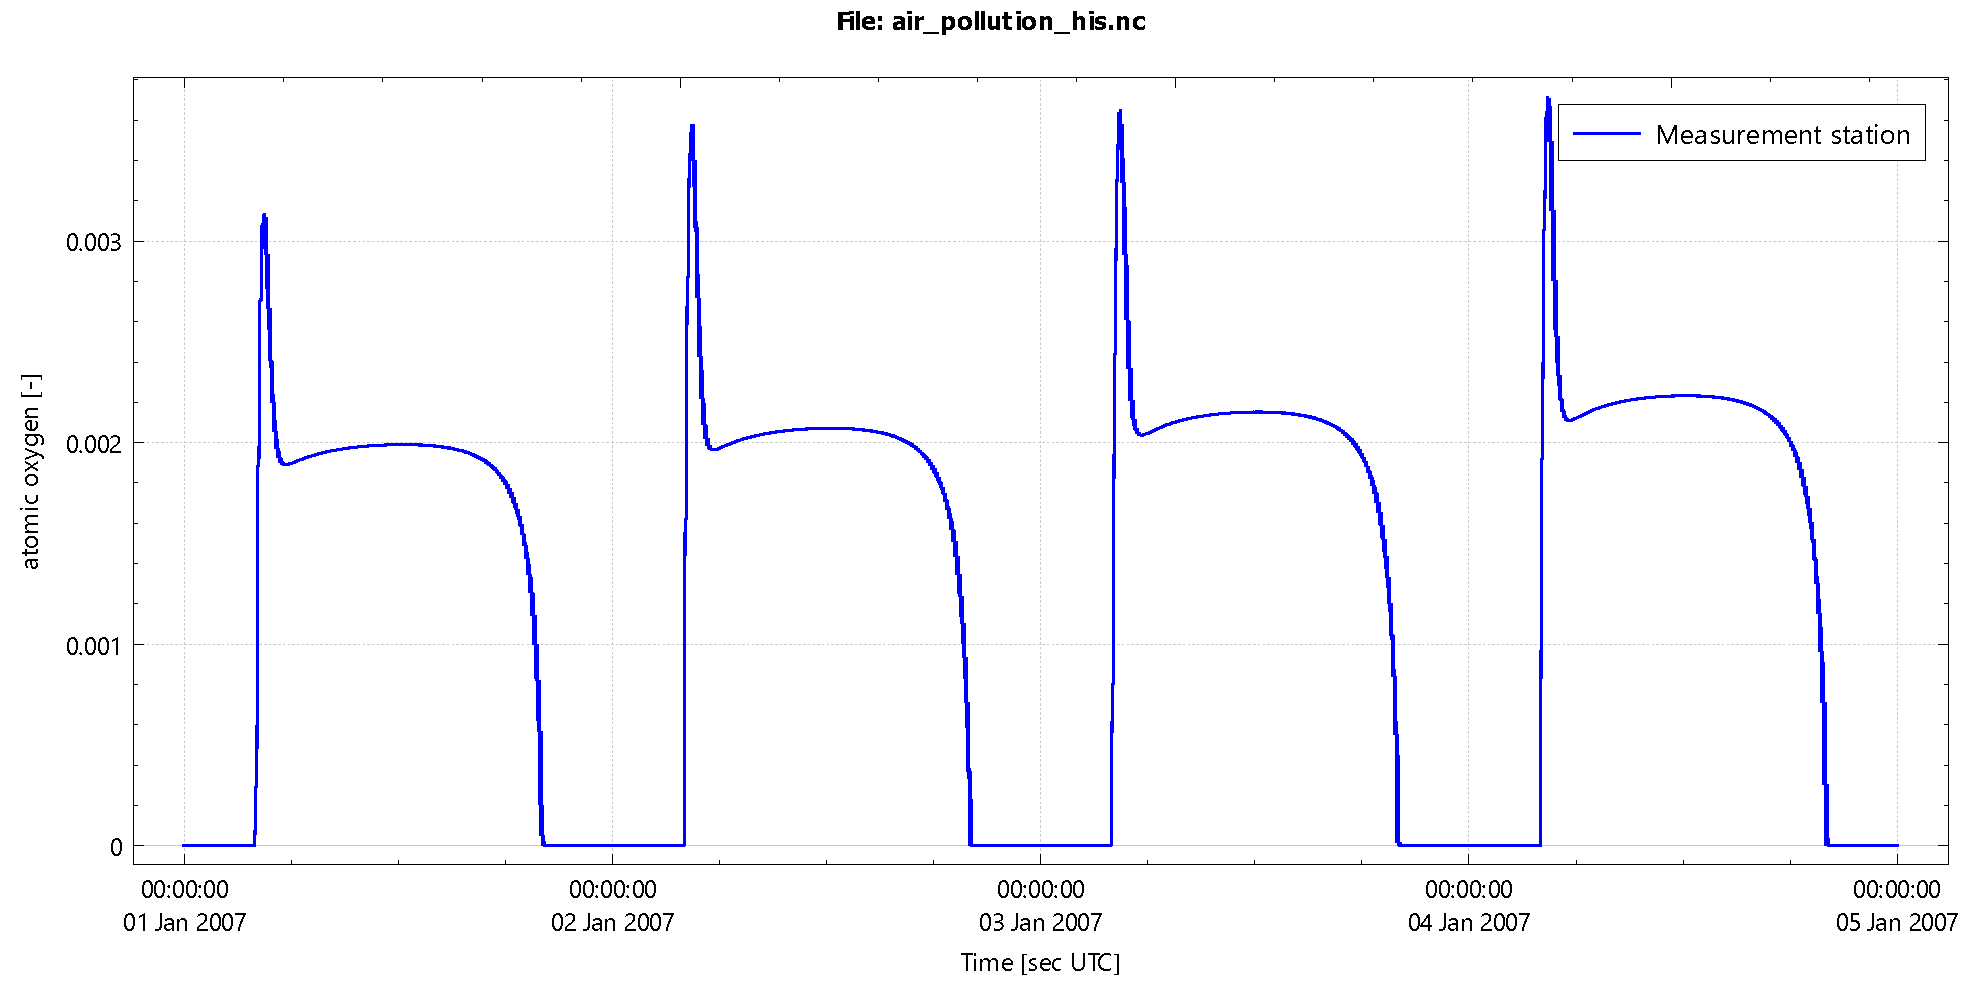
\includegraphics[width=\textwidth]{figures/atomic_oxygen_dt0d5.pdf}
        \caption{Concentration of Atomic Oxygen.}
    \end{subfigure}
    \begin{subfigure}{0.5\textwidth}
        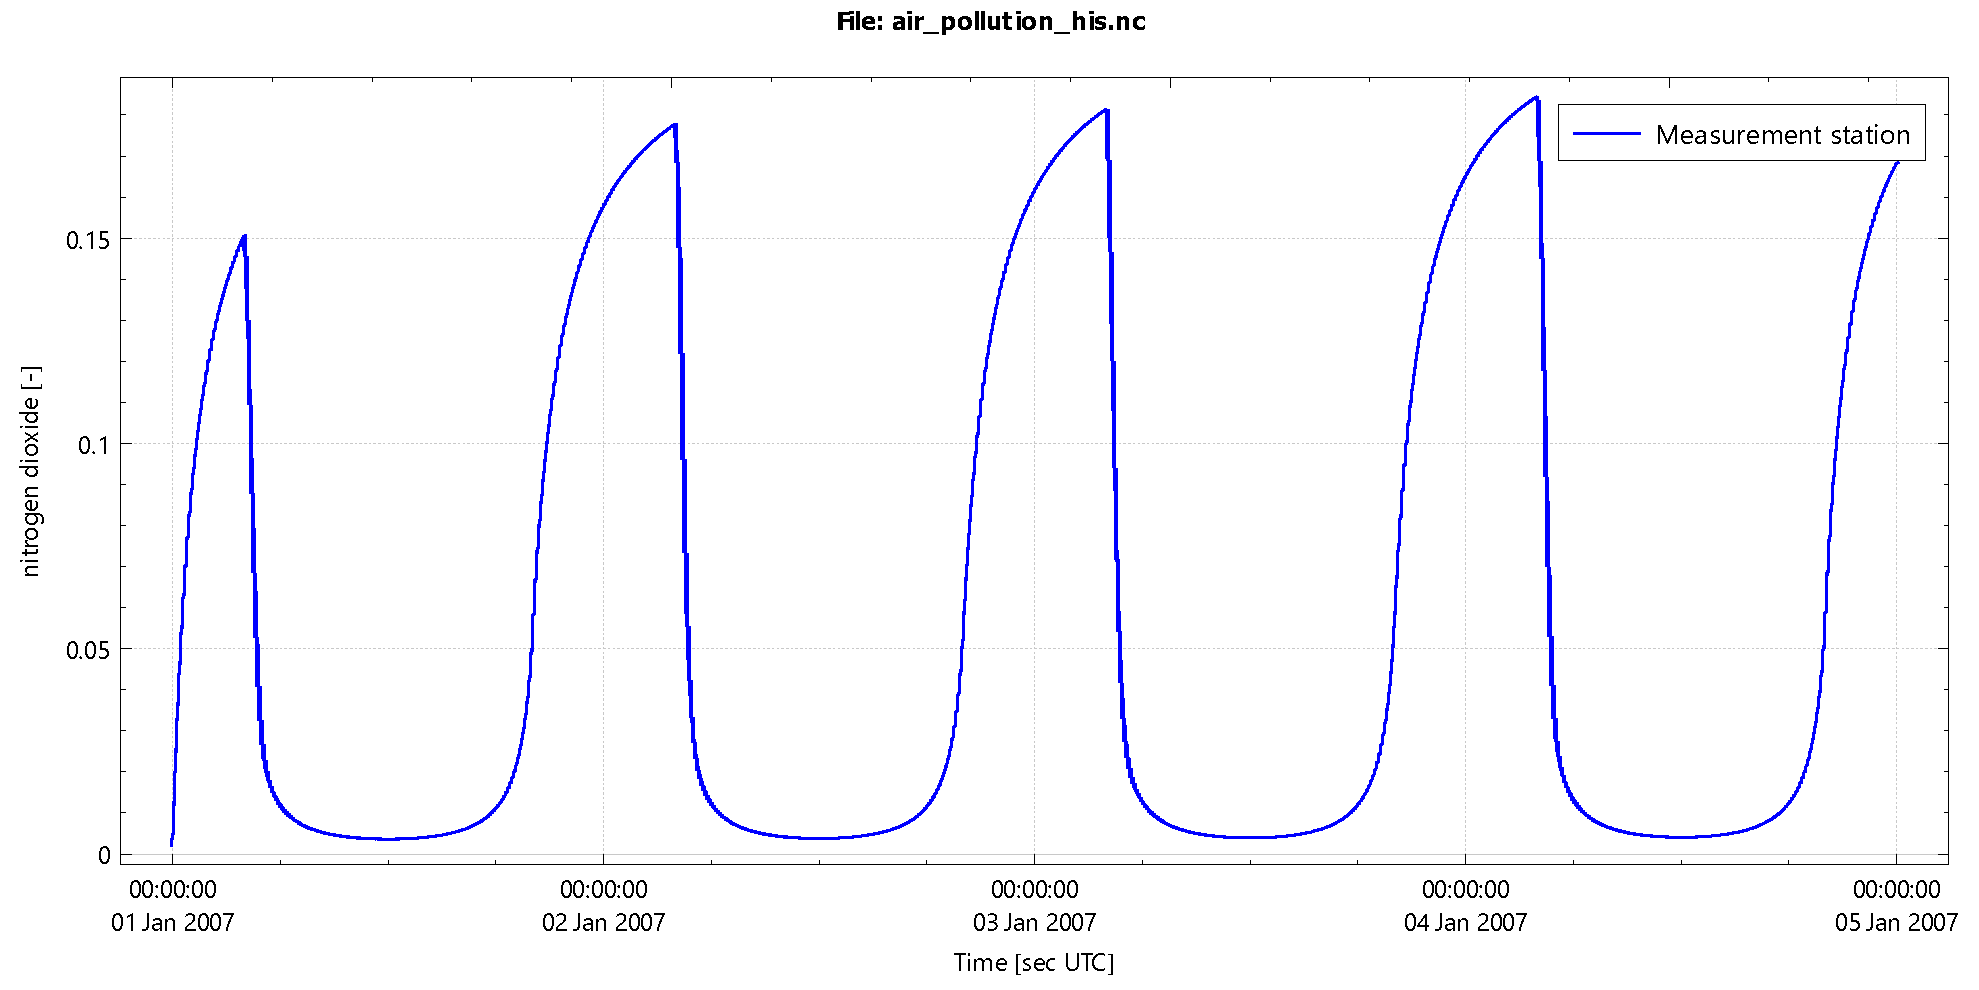
\includegraphics[width=\textwidth]{figures/nitrogen_dioxide_dt0d5.pdf}
        \caption{Concentration of Nitrogen Dioxide.}
    \end{subfigure}
    \begin{subfigure}{0.5\textwidth}
        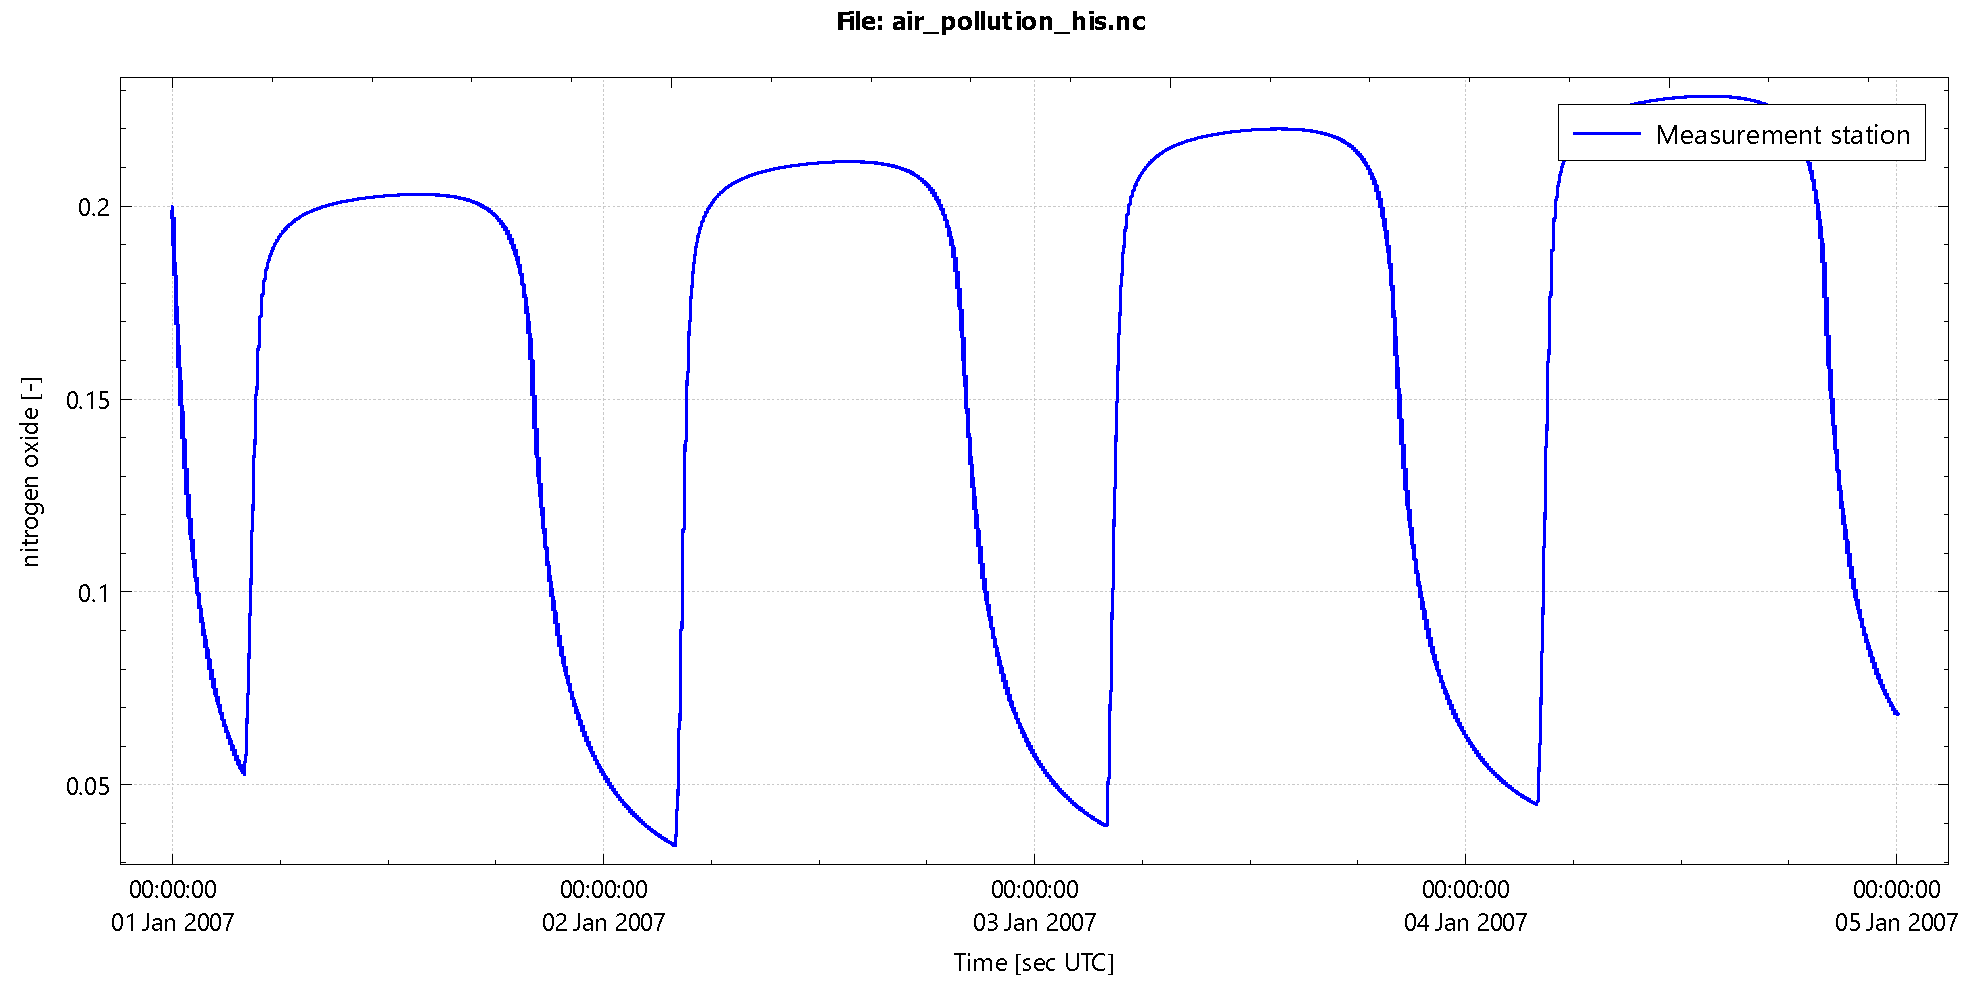
\includegraphics[width=\textwidth]{figures/nitrogen_oxide_dt0d5.pdf}
        \caption{Concentration of Nitrogen Oxide.}
    \end{subfigure}
    \begin{subfigure}{0.5\textwidth}
        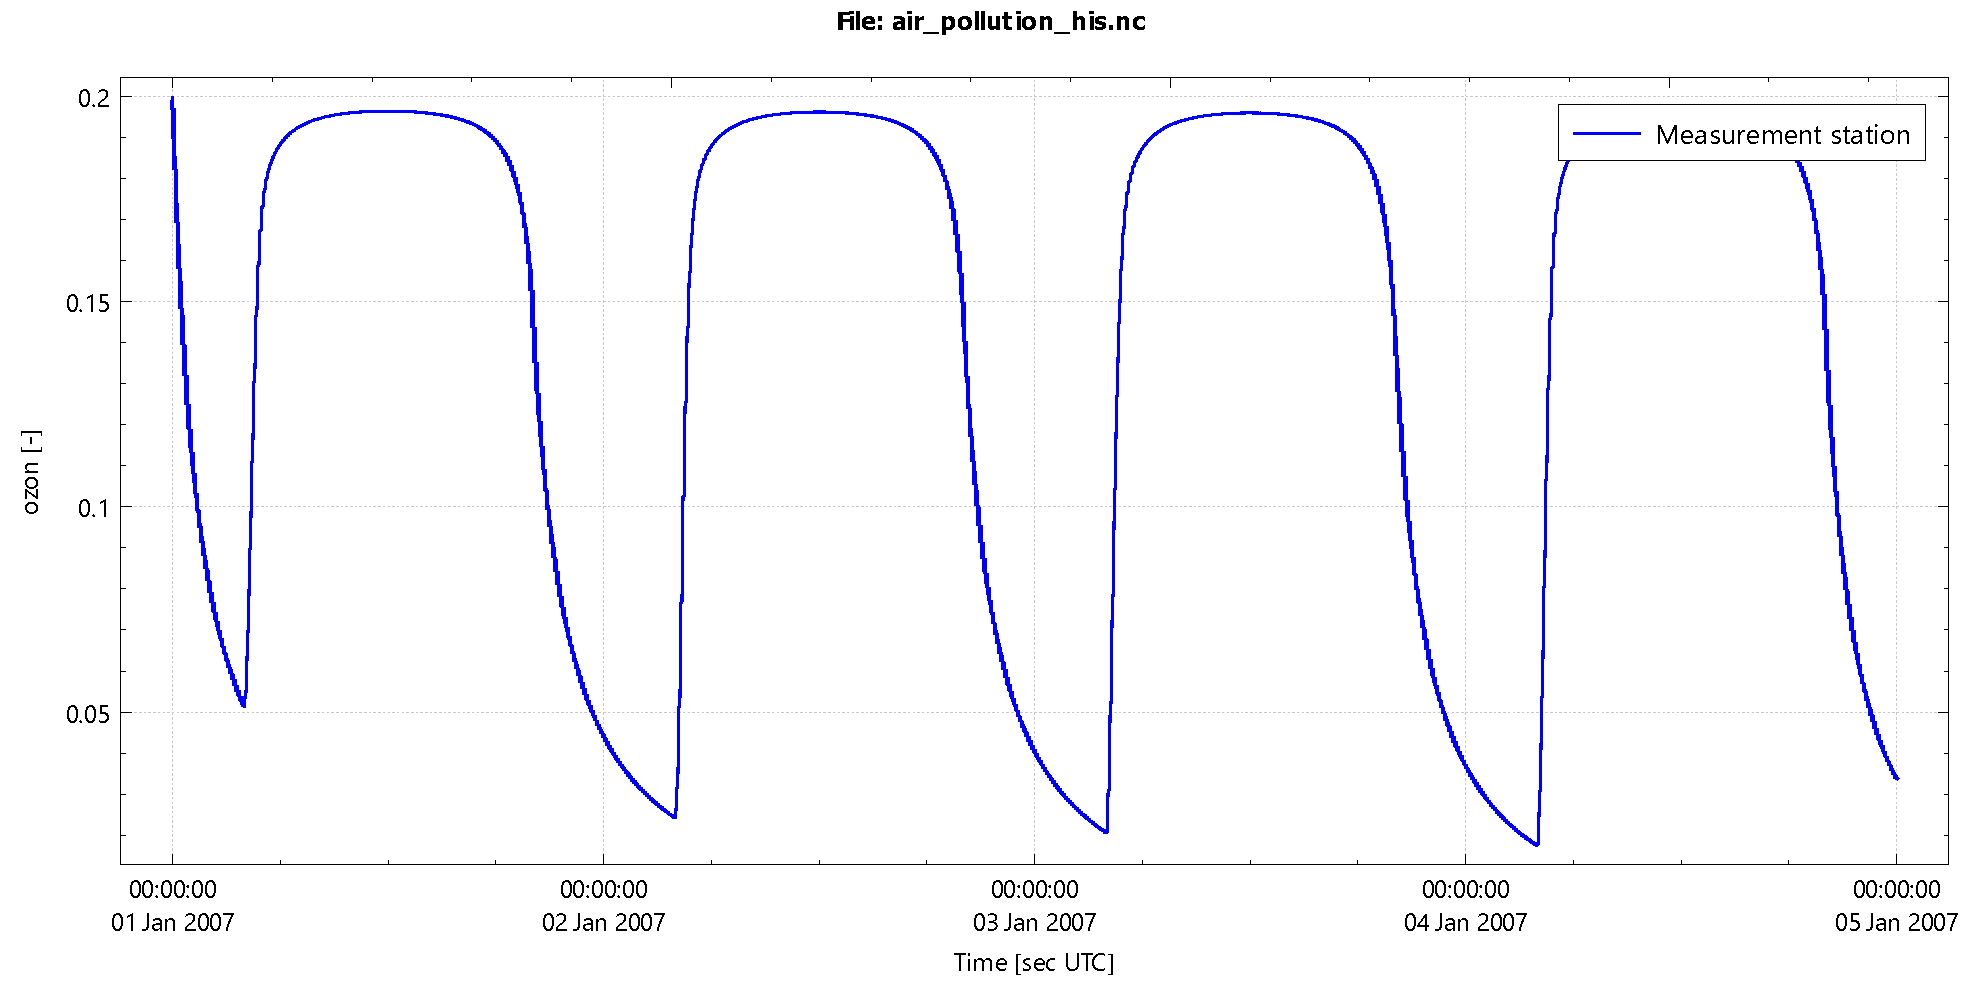
\includegraphics[width=\textwidth]{figures/ozon_dt0d5.pdf}
        \caption{Concentration of Ozon.}
    \end{subfigure}
    \caption[Air pollution experiment: $O$, $N_2$, $NO$ and $O_3$]{Result plots of the different constituents, compute with the fully implicit time integration method with a time step of \bqty{0.5}{\second}.}
\end{figure}

%------------------------------------------------------------------------------
\paragraph*{Different time integrators}
Numerical stability for different values of $\Dt$ are studied for Euler-explicit, Runga-Kutta-4 and the fully implicit $\Delta$-formulation.
%
\begin{longtable}{|>{\bfseries}p{6mm-12pt}|p{\textwidth/4-2mm-12pt}|p{\textwidth/4-2mm-12pt}|p{\textwidth/4-2mm-12pt}|p{\textwidth/4-2mm-12pt}|}
    \caption{Stability for different time integrators} \\%
    \rowcolor{mgreen1}
    & \textcolor{white}{\textbf{Time step\newline \bunit{\second}}}
    & \textcolor{white}{\textbf{Euler explicit}}
    & \textcolor{white}{\textbf{Runge-Kutta 4}}
    & \textcolor{white}{\textbf{Fully Implicit\newline \deltaformulation}}
    \\
    \topline
    \endfirsthead
    \rowcolor{mgreen1}
    & \textcolor{white}{\textbf{Time step\newline \bunit{\second}}}
    & \textcolor{white}{\textbf{Euler Explicit}}
    & \textcolor{white}{\textbf{Runge-Kutta 4}}
    & \textcolor{white}{\textbf{Fully Implicit\newline \deltaformulation}}
    \\
    \midline
    \endhead
    \endfoot
    \bottomline
    \endlastfoot
    1 & 0.5 & -  & \checkmark & \checkmark  \\
    \midline
    2 & 60 & \checkmark  & \checkmark  &  \checkmark \\
    \midline
    3 & 120 & Unstable & \checkmark &  \checkmark \\
    \midline
    4 & 180 & - & Unstable & \checkmark \\
    \midline
    5 & 240 & - & - & \checkmark \\
    \midline
    6 & 300 & - & - & \checkmark \\
    \midline
    7 & 900 & - & - & \checkmark \\
    \midline
    8 & 1800 & - & - & \checkmark \\
    \midline
    9 & 3600 & - & - & \checkmark \\
\end{longtable}

%
%------------------------------------------------------------------------------
\subsection{Brusselator}
%--------------------------------------------------------------------------------
Some numerical results of the brusselator example (\autoref{sec:brusselator}) is:
\begin{figure}[H]
    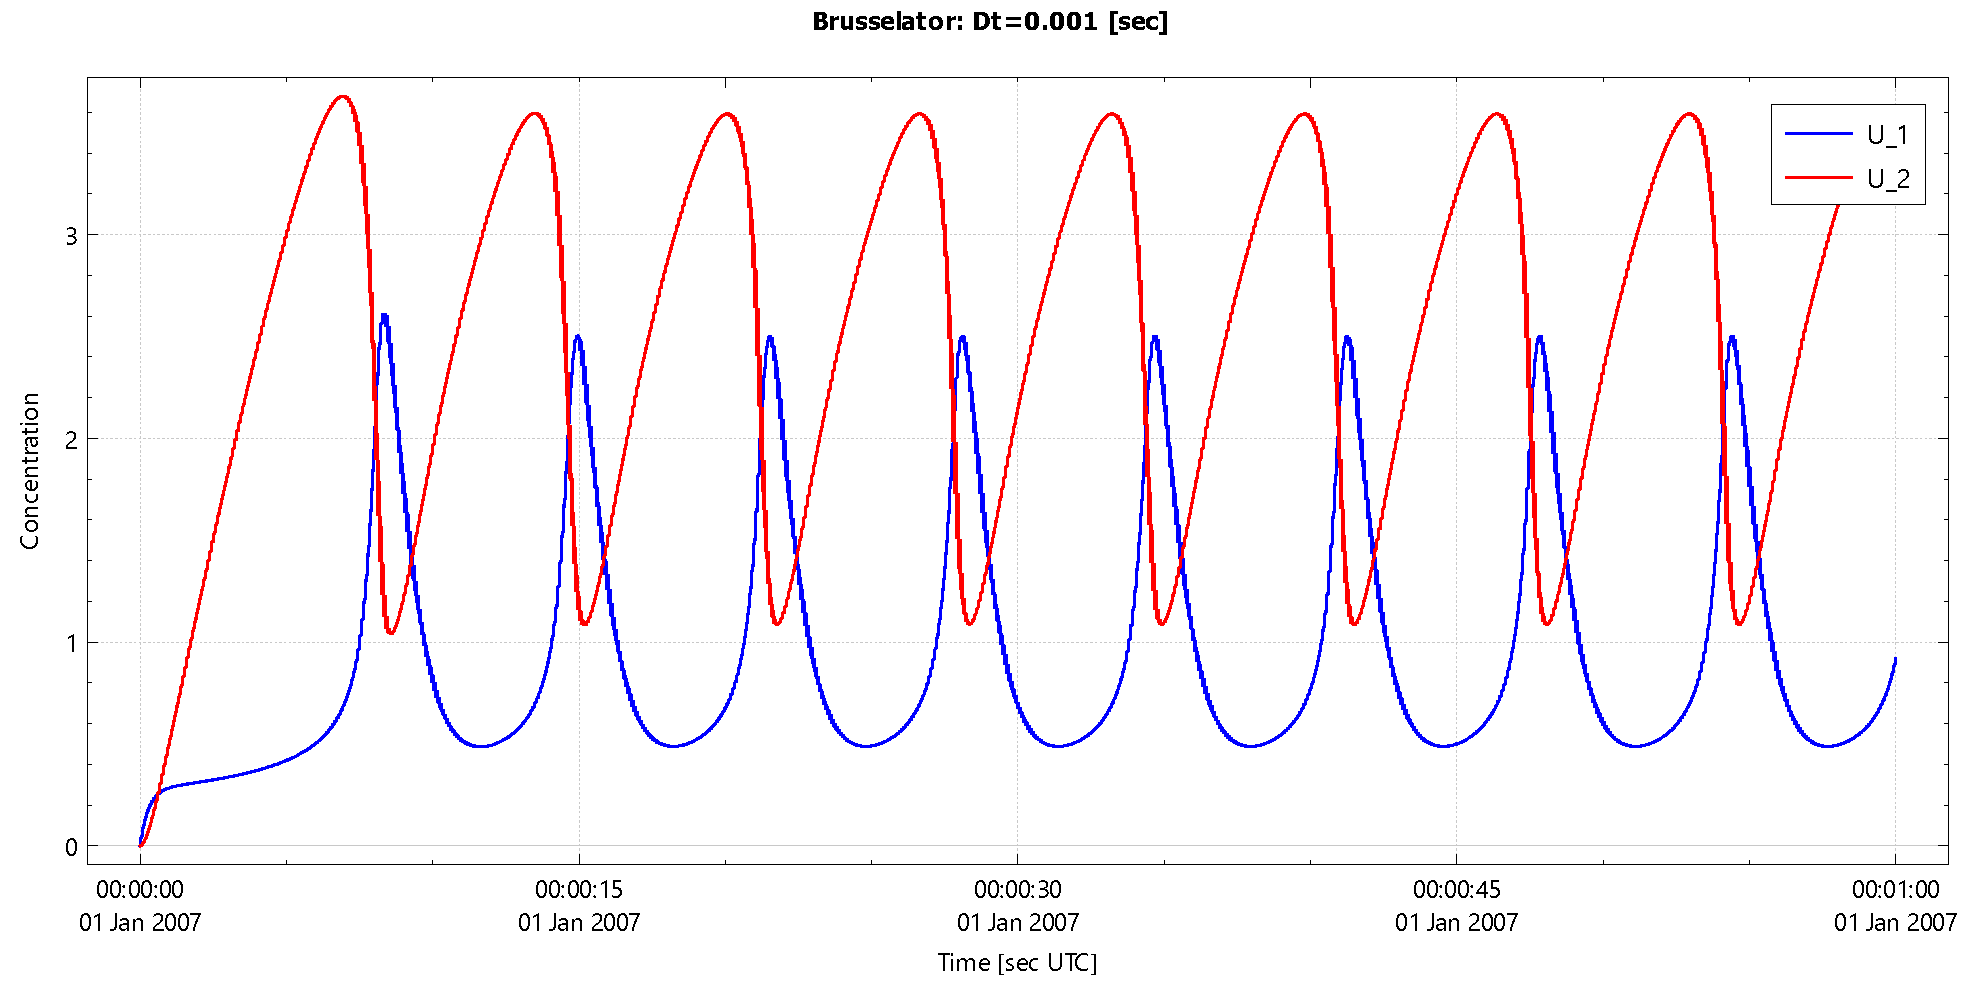
\includegraphics[width=\textwidth]{figures/brusselator_imp_dt=0d001.pdf}
    \caption[Brusselator experiment: $\Dt = 0.001\ \bunit{\second}$]{Fully Implicit: $\Dt=0.001$\ \bunit{\second}, $k_1=1$, $k_2=2.5$. }\label{fig:brusselator_reference}
\end{figure}
The solution presented in \autoref{fig:brusselator_reference} is assumed to be the reference (analytic) solution of \autoref{eq:brusselator}.
%
\begin{figure}[H]
    \begin{subfigure}{0.5\textwidth}
        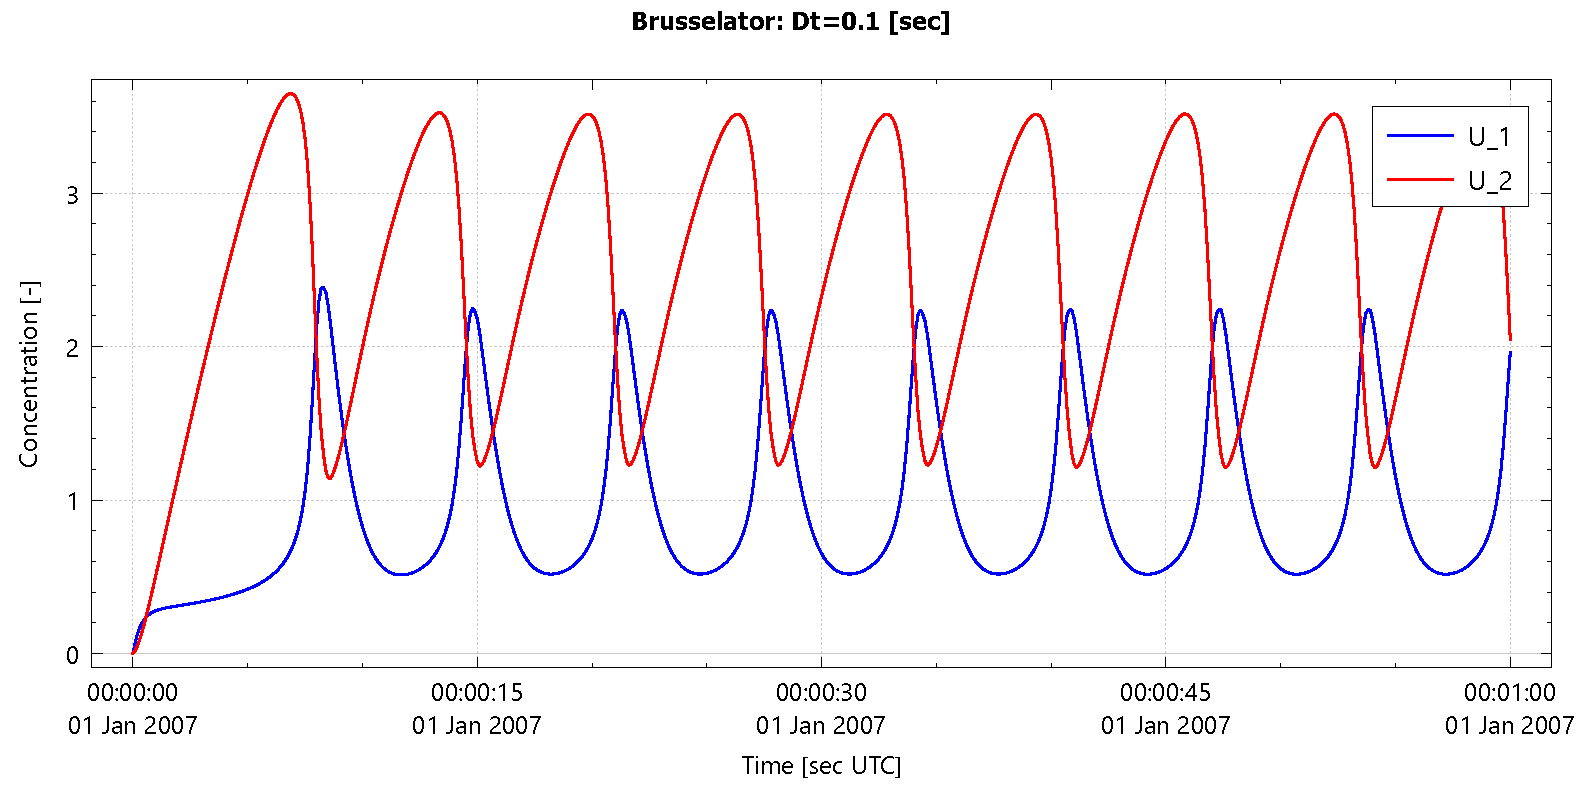
\includegraphics[width=\textwidth]{figures/brusselator_imp_dt=0d10.pdf}
        \caption{Fully Implicit: $\Dt=\bqty{0.1}{\second}$, $k_1=1$, $k_2=2.5$}
    \end{subfigure}
    \begin{subfigure}{0.5\textwidth}
        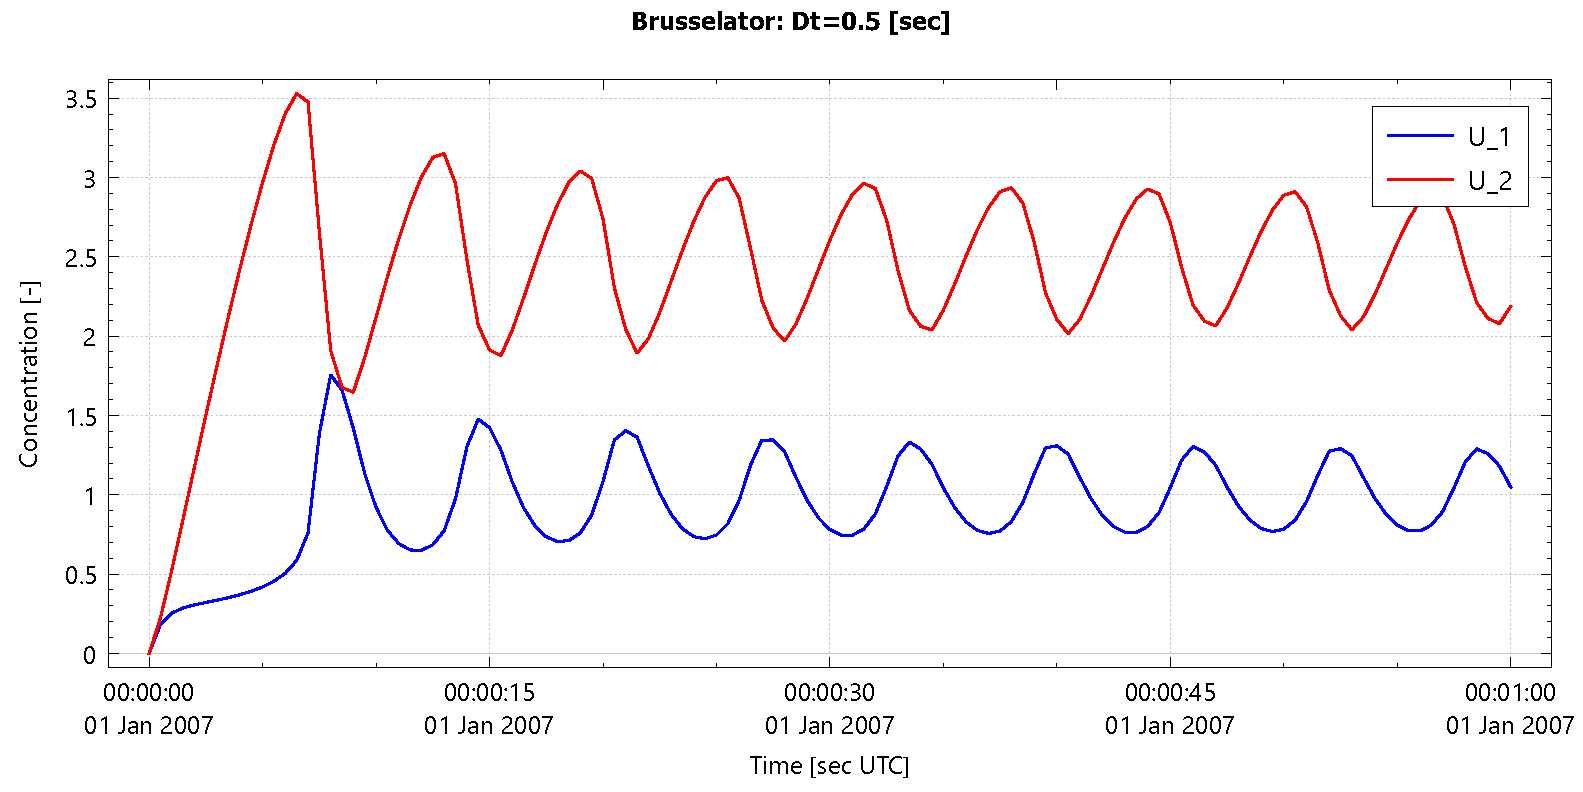
\includegraphics[width=\textwidth]{figures/brusselator_imp_dt=0d50.pdf}
        \caption{Fully Implicit: $\Dt=\bqty{0.5}{\second}$, $k_1=1$, $k_2=2.5$}
    \end{subfigure}
    \caption[Brusselator experiment: $\Dt = 0.1, 0.5\ \bunit{\second}$]{Result plots for constant value of $k_1 = 1$ and $k_2 =2.5$, computed with a fully implicit ($\Delta$ formulation) time integration method for different time steps $\Dt = 0.1, 0.5\ \bunit{\second}$.}
\end{figure}
Extra attention is needed for the Fully Implicit time integration with larger time step:
\begin{figure}[H]
    \begin{subfigure}{0.5\textwidth}
        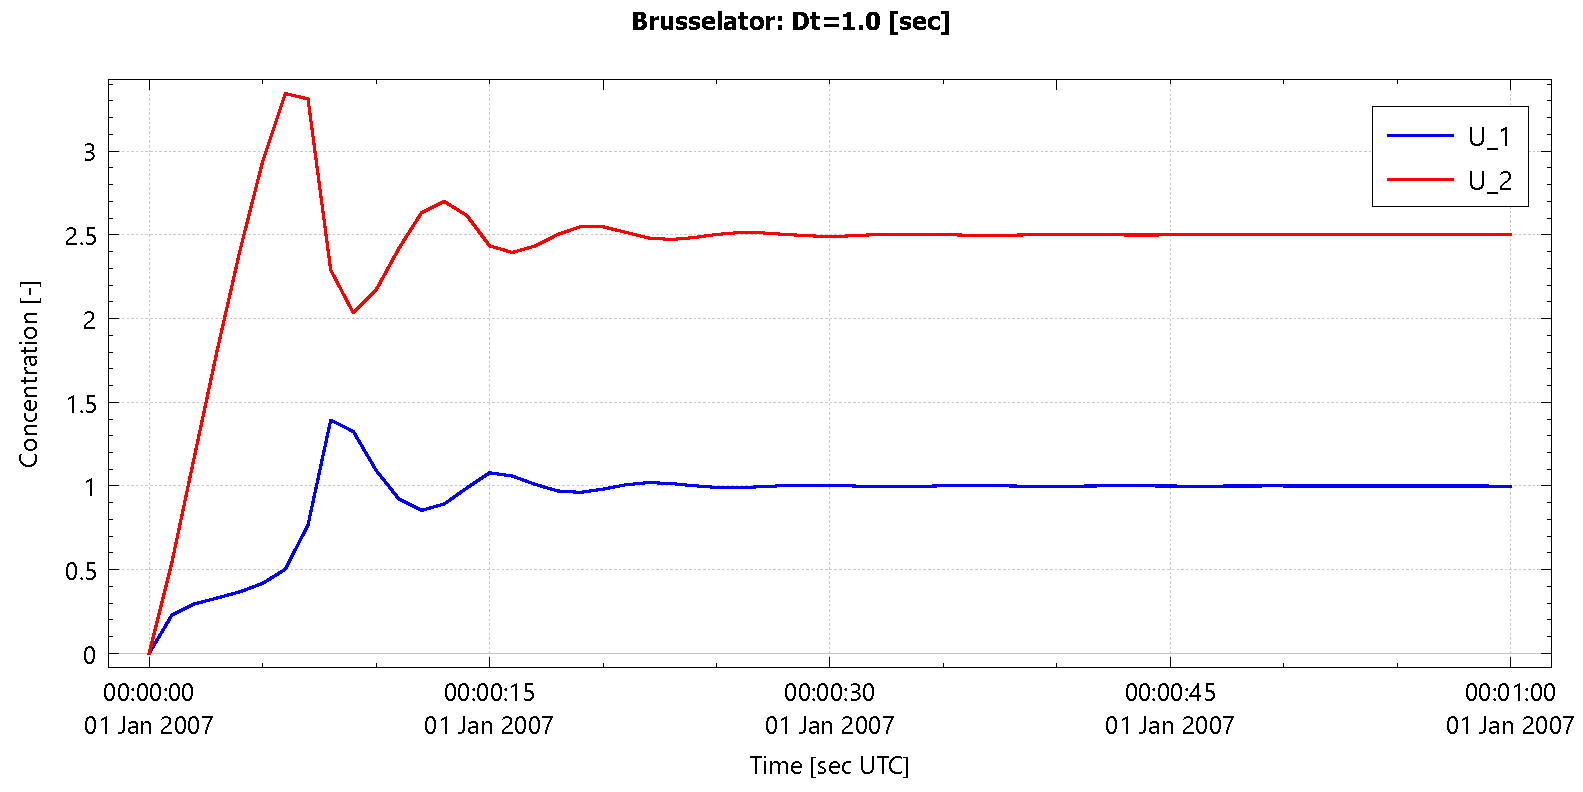
\includegraphics[width=\textwidth]{figures/brusselator_imp_dt=1d00.pdf}
        \caption{Fully Implicit: $\Dt=\bqty{1.0}{\second}$, $k_1=1$, $k_2=2.5$}\label{fig:imp_dt=1d00}
    \end{subfigure}
    \begin{subfigure}{0.5\textwidth}
        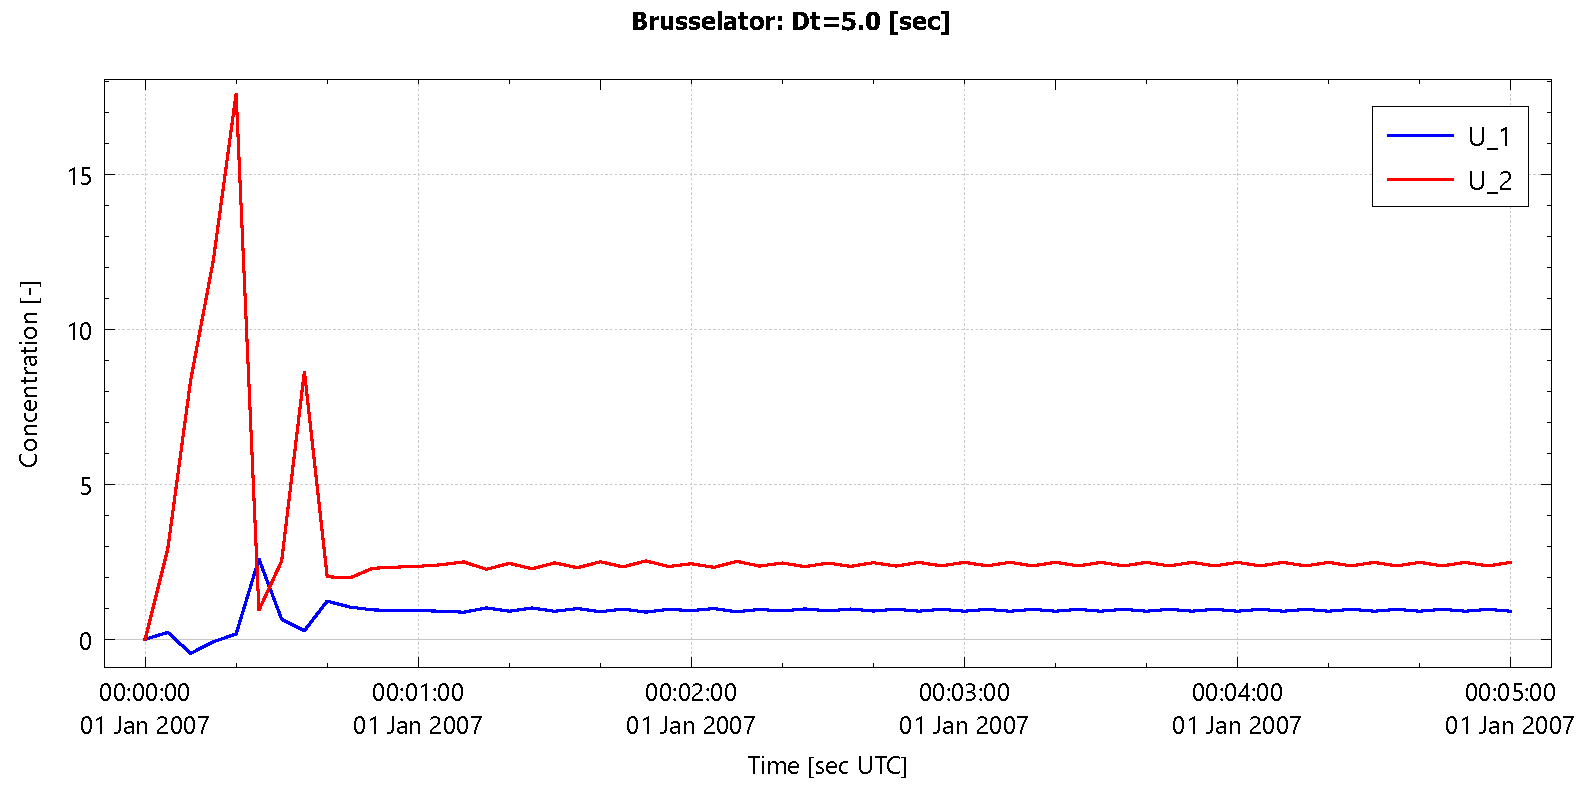
\includegraphics[width=\textwidth]{figures/brusselator_imp_dt=5d00.pdf}
        \caption{Fully Implicit: $\Dt=\bqty{5.0}{\second}$, $k_1=1$, $k_2=2.5$}\label{fig:imp_dt=5d00}
    \end{subfigure}
    \caption[Brusselator experiment: $\Dt = 1.0, 5.0\ \bunit{\second}$]{Result plots for constant value of $k_1 = 1$ and $k_2 =2.5$, computed with a fully implicit ($\Delta$ formulation) time integration method for different time steps $\Dt = 1.0, 5.0\ \bunit{\second}$.
    }
\end{figure}
\Autoref{fig:imp_dt=1d00} converge to the equilibrium state $(u_1, u_2) = (1.0, 2.5)$ and
\Autoref{fig:imp_dt=5d00} looks to converge to the equilibrium state $(u_1, u_2) = (1.0, 2.5)$ but is still wiggling after \bqty{5}{\minute} of simulation time (even after one day --- not presented here).
How these equations are discretized is given in \autoref{sec:brusselator_discretization}.

%------------------------------------------------------------------------------
\paragraph*{Different time integrators}
Numerical stability for different values of $\Dt$ are studied for the Runga-Kutta-4 and fully implicit \deltaformulation.
%
\begin{longtable}{|>{\bfseries}p{6mm-12pt}|p{\textwidth/3-2mm-12pt}|p{\textwidth/3-2mm-12pt}|p{\textwidth/3-2mm-12pt}|}
    \caption{Stability of different time integrators for the Brusselator.} \\%
    \rowcolor{mgreen1}
    & \textcolor{white}{\textbf{Time step\newline \bunit{\second}}}
    & \textcolor{white}{\textbf{Runge-Kutta 4}}
    & \textcolor{white}{\textbf{Fully Implicit\newline \deltaformulation}}
    \\
    \topline
    \endfirsthead
    \rowcolor{mgreen1}
    & \textcolor{white}{\textbf{Time step\newline \bunit{\second}}}
    & \textcolor{white}{\textbf{Runge-Kutta 4}}
    & \textcolor{white}{\textbf{Fully Implicit\newline \deltaformulation}}
    \\
    \midline
    \endhead
    \endfoot
    \bottomline
    \endlastfoot
    1 & 0.1 & \checkmark & \checkmark  \\
    \midline
    2 & 0.2  & \checkmark &  \checkmark   \\
    \midline
    3 & 0.5 & \checkmark &  \checkmark   \\
    \midline
    4 & 1.0 & Unstable &   \checkmark  \\
    \midline
    5 & 2.0 &   &   \checkmark  \\
    \midline
    6 & 5.0 &   &   \checkmark  \\
    \midline
\end{longtable}


%--------------------------------------------------------------------------------
\section{1-D Advection equation}
The considered advection equation reads:
\begin{align}
    \pdiff{c}{t} + \pdiff{uc}{x} = 0,
\end{align}
With a velocity of $u = \bqty{10}{\metre\per\second}$, which coincide with the wave celerity of the 1D-wave numerical experiments as described in \autoref{sec:numerical_experiment}.
\begin{align}
    u(x,t) = \bqty{10}{\metre\per\second}
\end{align}
and with a prescribed boundary condition at the left side of the domain
\begin{align}
    c(0,t) = f_c(t).
\end{align}
%--------------------------------------------------------------------------------
\subsection{Transport of a constant constituent at the boundary} \label{sec:numerical_experiment_1d_adv_constant_boundary}
The prescribed boundary condition for the constituent reads
% reg_factor = 0.5 * (std::cos(M_PI * (treg - double(nst) * dt) / treg) + 1.0);
\begin{align}
    c(0,t) = c_{\it given}
    \begin{cases}
        \half \left(\cos\left(\pi \frac{t_{reg} - t}{t_{reg}} \right) + 1\right) &\quad \text{if } t < t_{reg},
        \\
        1 &\quad \text{if } t \geq t_{reg},
    \end{cases}
    \label{eq:1d_adv_boundary_condition}
\end{align}
where
\begin{symbollist}
    \item[$t_{reg}$] The regularization time for the given time-series, [\si{\second}]
    \nomenclature{$t_{reg}$}{\si{\second}}{The regularization time for the given time-series}
\end{symbollist}
%--------------------------------------------------------------------------------
\paragraph*{Numerical experiment}
The numerical experiment is performed with the following parameters:
\begin{itemize}
    \item Length of the domain, $L_x = \bqty{12000}{\metre}$
    \item Grid size, $\Dx = \bqty{10}{\metre}$
    \item Start time, $t_{start} = \bqty{0}{\second}$
    \item End time, $t_{stop} = \bqty{3600}{\second}$
    \item Timestep, $\Dt = \bqty{5}{\second}$
    \item Regularization time for time-series, $t_{reg} = \bqty{600}{\second}$
    \item Prescribed constant velocity, $u_{\it given}(x,t) = \bqty{10}{\metre\per\second}$
    \item Prescribed initial value of the constituent, $c(x,0)= \bqty{0}{-}$.
    \item Prescribed constituent on boundary at $x=0$ is given by \autoref{eq:1d_adv_boundary_condition}.
    \item No boundary is prescribed at $x=\bqty{12000}{\metre}$.
\end{itemize}
%--------------------------------------------------------------------------------
\paragraph*{Results of the numerical experiments}
A map picture at $t=\bqty{3600}{\second}$ and time-series are given for this experiment.
As seen from the map figure there are very small spurious waves traveling from right to left.
These spurious waves are fully generated by the numerical scheme at the right boundary,
because the continuous advection equation does \textbf{not} allow information traveling from right to left.
\begin{figure}[H]
    \centering
    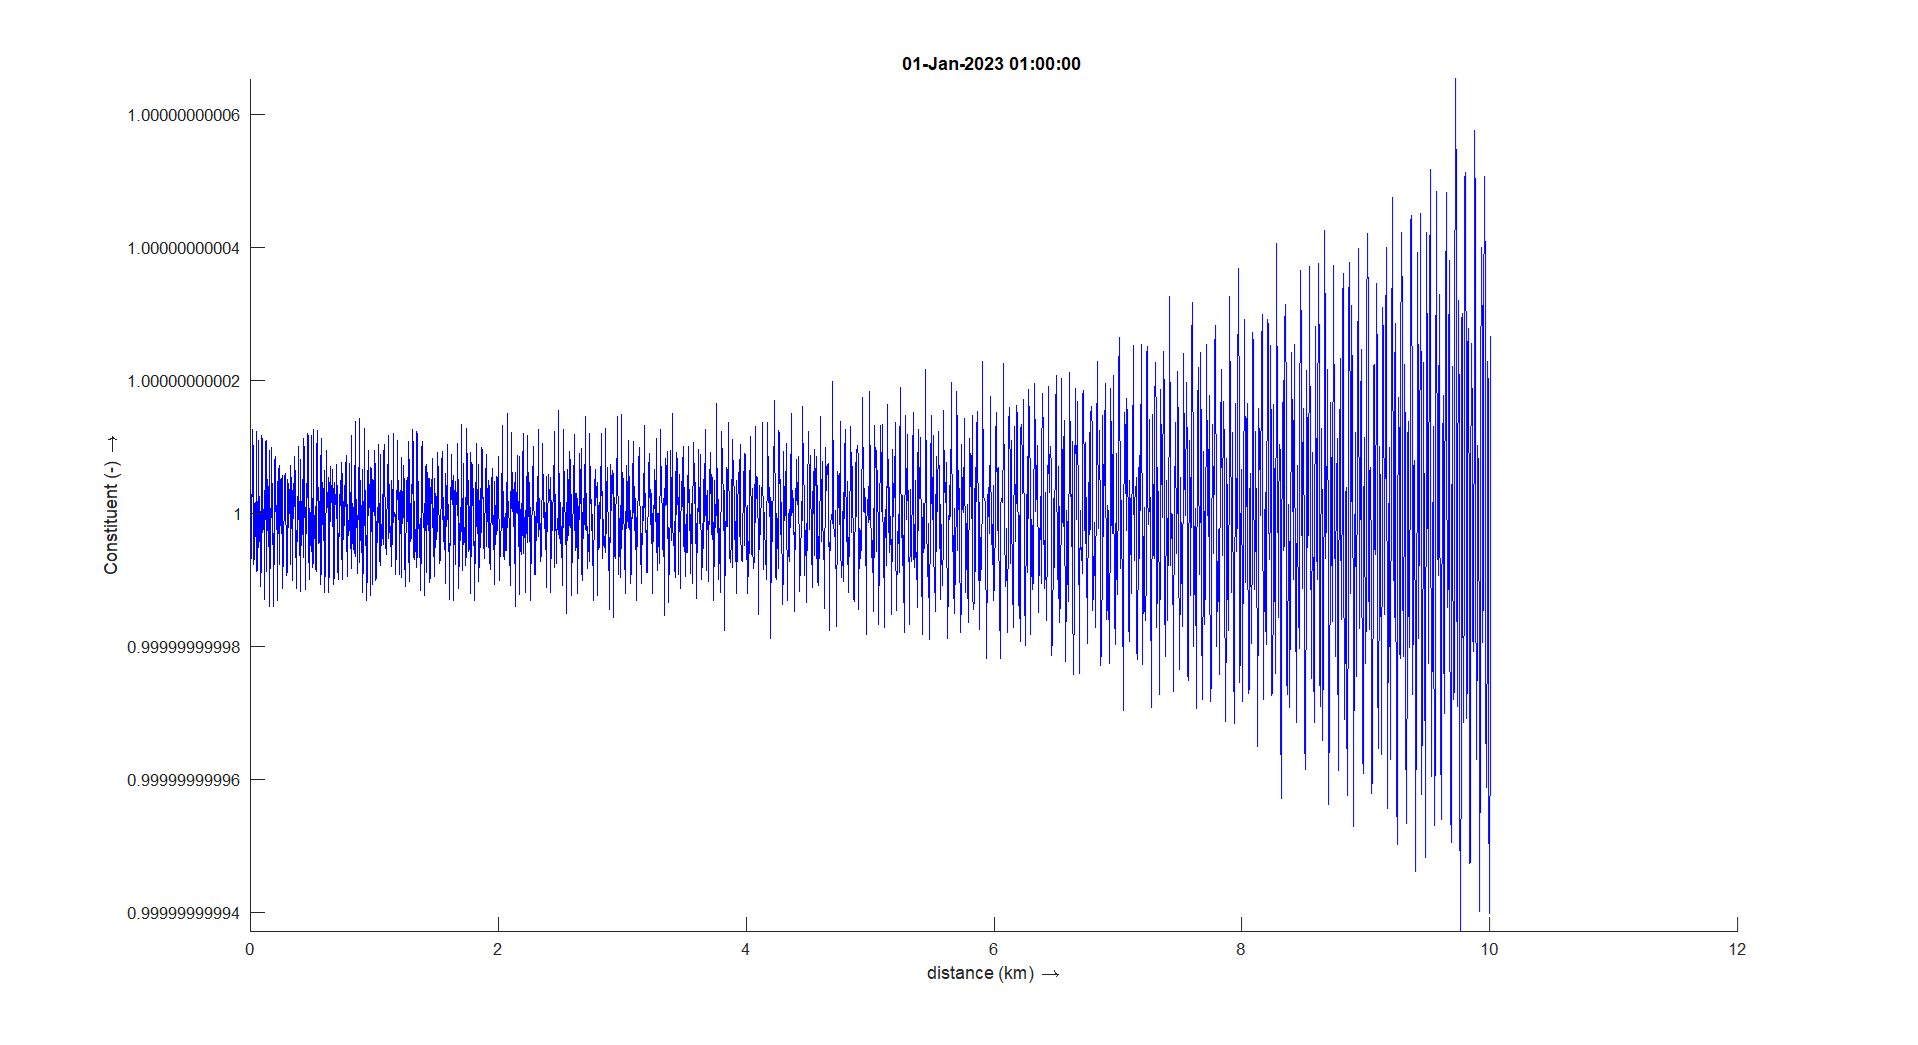
\includegraphics[width=0.9\textwidth]{figures/constant_3600s.png}
    \caption{Spurious waves at $t=\bqty{3600}{\second}$. Range from $ 1 \pm \num{8e-09}$.}
\end{figure}
Results for several observation stations along the channel are shown in \autoref{fig:result_1d_adv_constant_bc}
\begin{figure}[H]
    \centering
    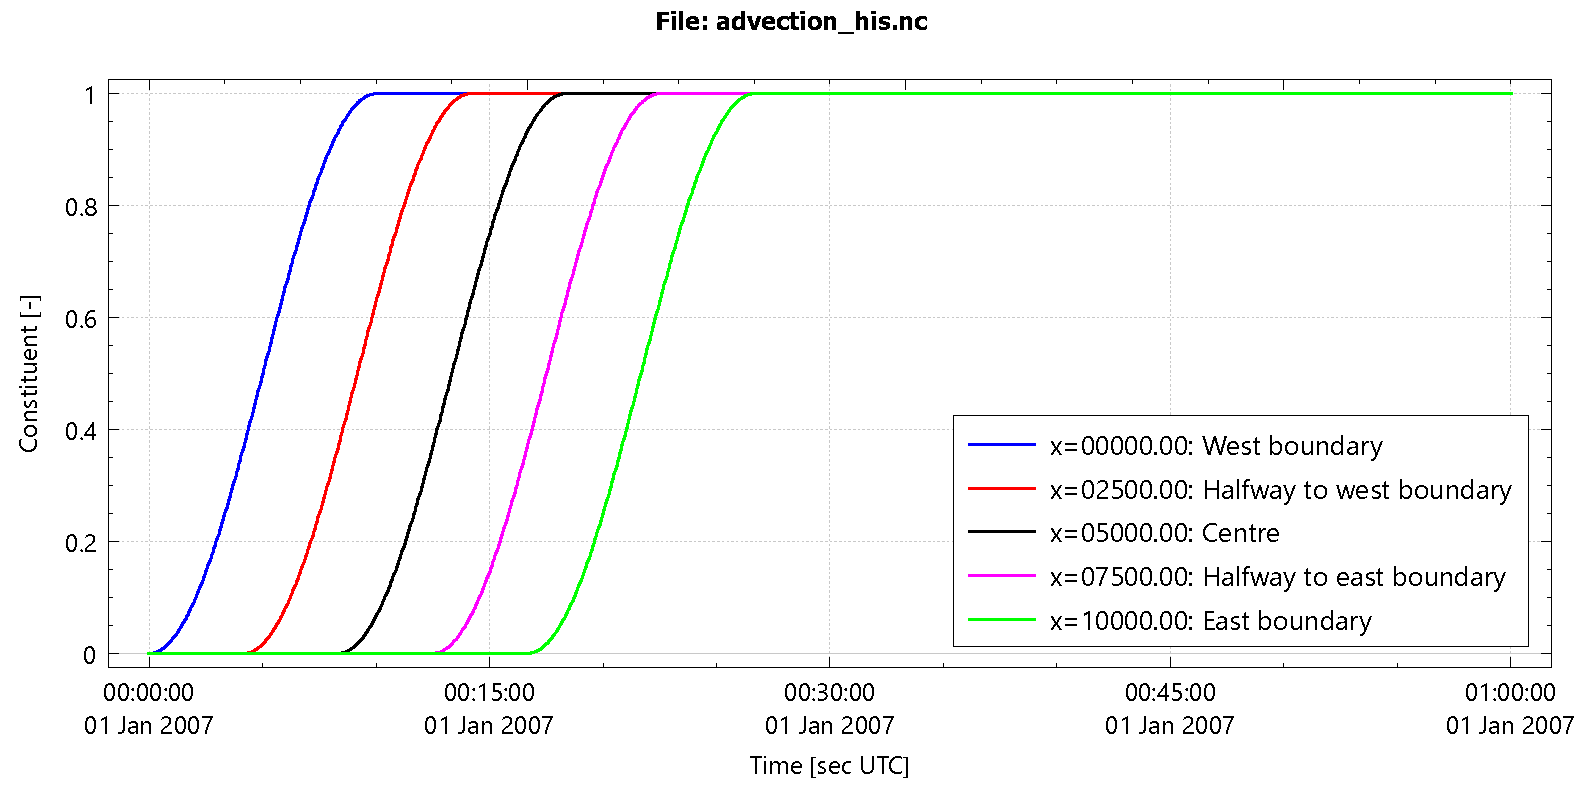
\includegraphics[width=0.9\textwidth]{figures/time-series-advection-constant.pdf}
    \caption{Time-series for several stations in the model, showing the transition behavior between the initial situation and the time-independent solution.}
    \label{fig:result_1d_adv_constant_bc}
\end{figure}
%--------------------------------------------------------------------------------
\subsection{Transport of a time-dependent constituent at the boundary}
\label{sec:numerical_experiment_1d_adv_time_dependent_boundary}
The prescribed boundary condition for the constituent reads
% reg_factor = 0.5 * (std::cos(M_PI * (treg - double(nst) * dt) / treg) + 1.0);
\begin{align}
    c(0,t) = c_{\it given}
    \begin{cases}
        \half \left(\cos\left(\pi \frac{t_{reg} - t}{t_{reg}}\right) + 1  \right) &\quad \text{if } t < t_{reg},
        \\
        -\cos\left(\pi \frac{t}{t_{\it reg}} \right) &\quad \text{if } t \geq t_{reg},
    \end{cases}
    \label{eq:1d_adv_sine_boundary_condition}
\end{align}
where
\begin{symbollist}
    \item[$t_{reg}$] The regularization time for the given time-series, [\si{\second}]
    \nomenclature{$t_{reg}$}{\si{\second}}{The regularization time for the given time-series}
\end{symbollist}
%--------------------------------------------------------------------------------
\paragraph*{Numerical experiment}
The numerical experiment is performed with the following parameters:
\begin{itemize}
    \item Length of the domain, $\bqty{12000}{\metre}$
    \item Grid size, $\Dx = \bqty{10}{\metre}$
    \item Start time, $t_{start} = \bqty{0}{\second}$
    \item End time, $t_{stop} = \bqty{3600}{\second}$
    \item Timestep, $\Dt = \bqty{10}{\second}$
    \item Regularization time for time-series, $t_{reg} = \bqty{600}{\second}$
    \item Prescribed constant velocity, $u_{\it given}(x,t) = \bqty{10}{\metre\per\second}$
    \item Prescribed initial value of the constituent, $c(x,0)= \bqty{0}{-}$.
    \item Prescribed constituent on boundary at $x=0$ is given by \autoref{eq:1d_adv_boundary_condition}.
    \item No boundary is prescribed at $x=\bqty{12000}{\metre}$.
\end{itemize}
%--------------------------------------------------------------------------------
\paragraph*{Results of the numerical experiments}
Results for several observation stations along the channel are shown in  \autoref{fig:result_1d_adv_sine_bc}:
\begin{figure}[H]
    \centering
    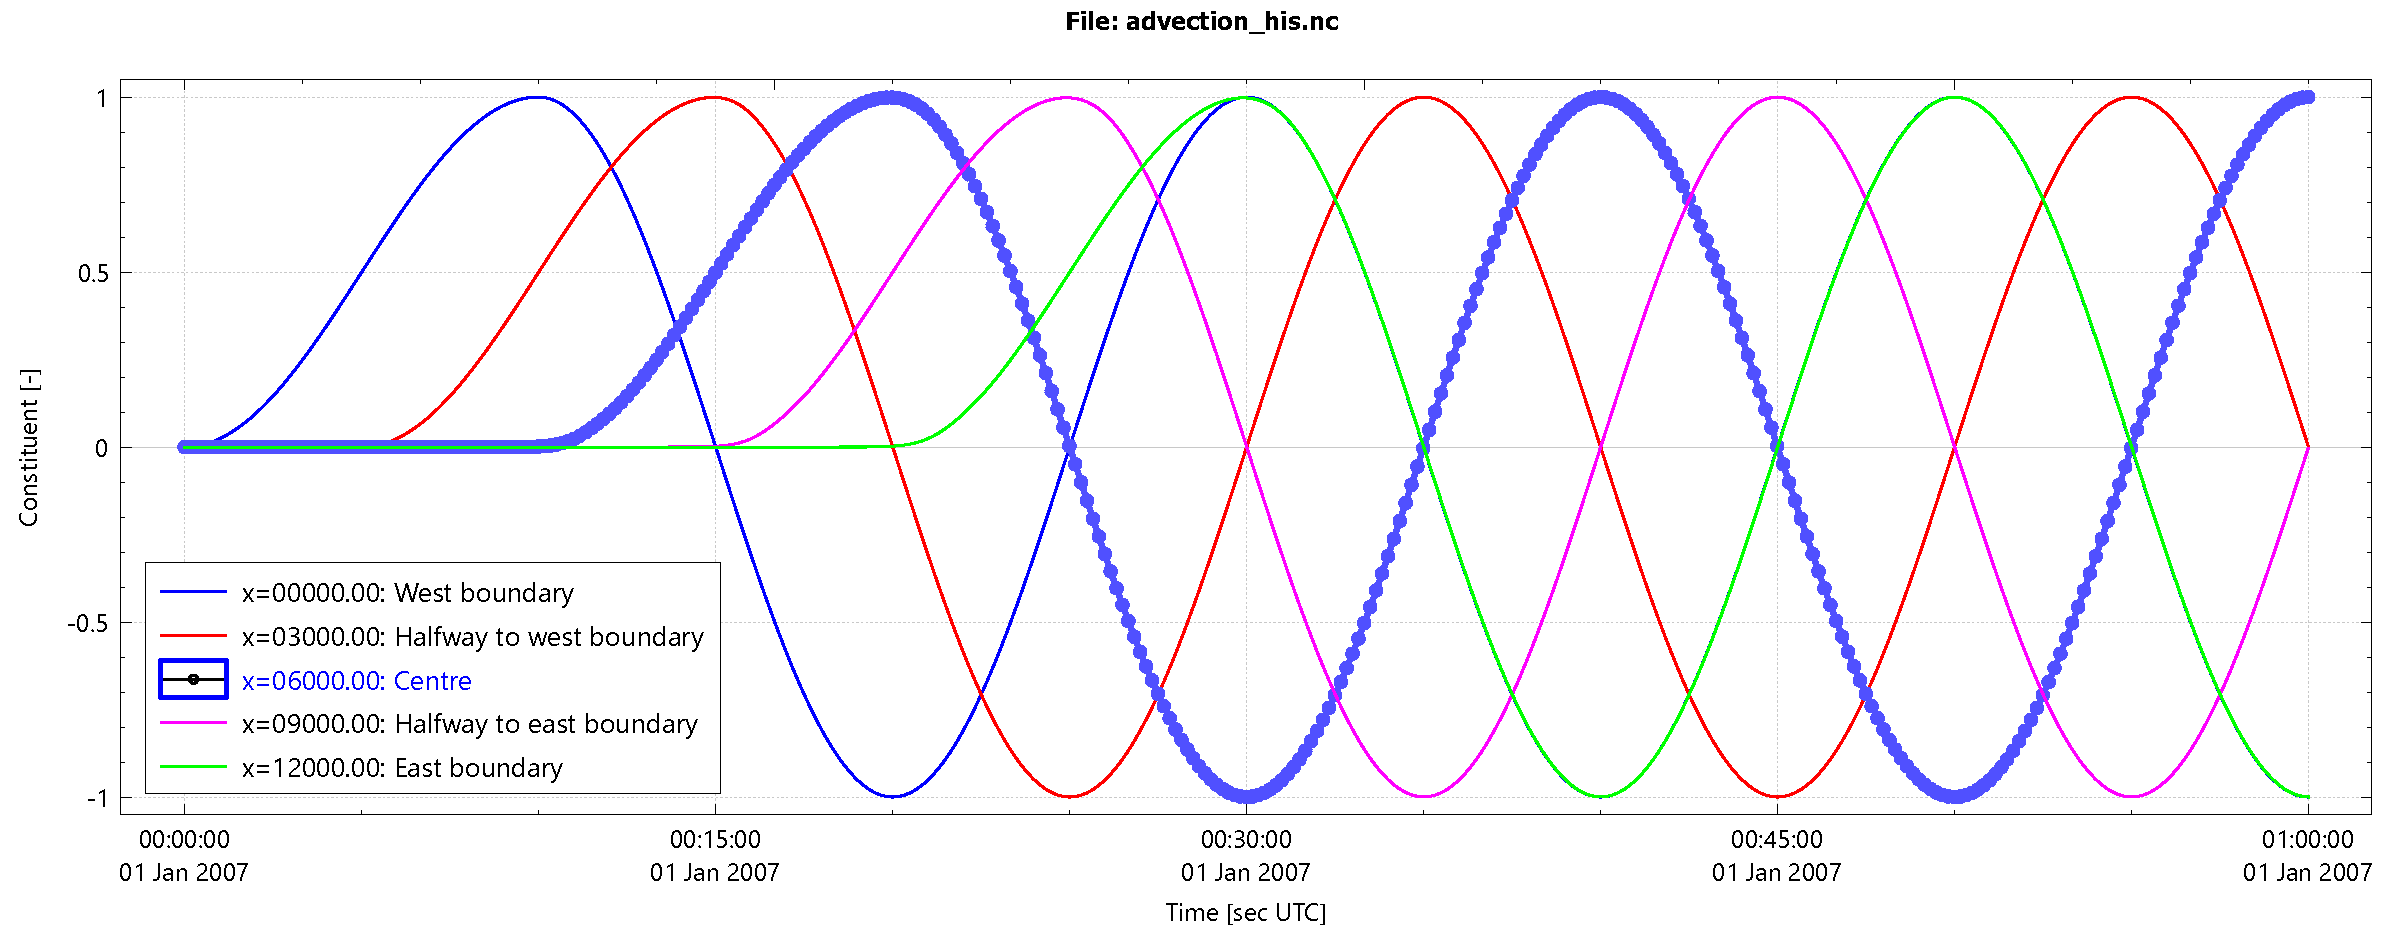
\includegraphics[width=0.9\textwidth]{figures/1d_advec_sine_dx10d0.pdf}
    \caption{Time-series for several stations in the model, showing the transition behavior between the initial situation and the time-independent solution.}
    \label{fig:result_1d_adv_sine_bc}
\end{figure}
%--------------------------------------------------------------------------------
\subsection{Transport of a wave package inside the domain}
The initial condition are computed as described in \autoref{sec:compatible_initialization}
and is illustrated in \autoref{fig:1d_adv_initial_wave_package}:
\begin{figure}[H]
    \centering
    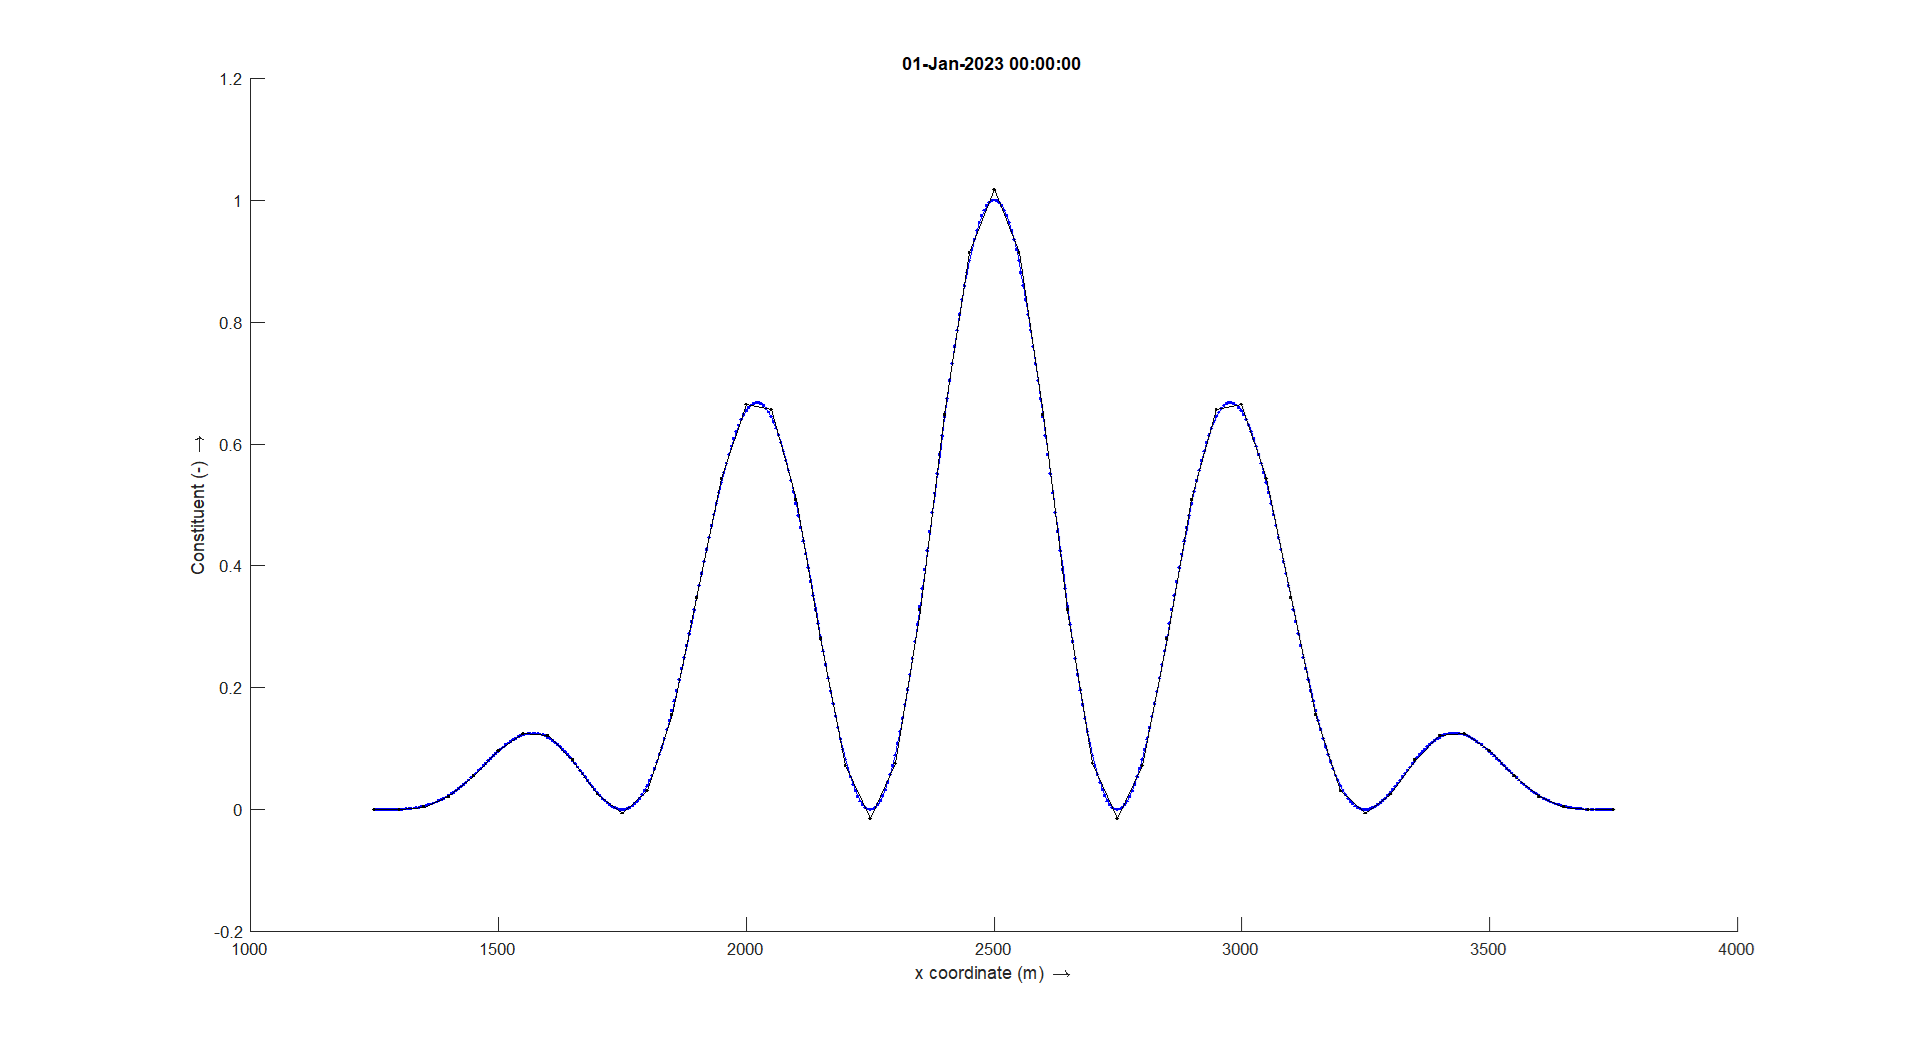
\includegraphics[width=0.9\textwidth]{figures/wave_package_000s.png}
    \caption{Compatible initial condition of the wave package. Blue: Initial condition when  $\Dx=\bqty{5}{\metre}$, Black: Initial condition when  $\Dx=\bqty{50}{\metre}$.}
    \label{fig:1d_adv_initial_wave_package}
\end{figure}
The graphs in \autoref{fig:1d_adv_initial_wave_package} do not coincide on the grid points because the profiles are computed according \autoref{sec:compatible_initialization}.
The initial condition is defined by:
\begin{align}
    u_{it given} =
    \begin{cases}
        0, & 0 < 1250, \bunit{\metre} \\
        \left(\half + \half \cos( 5k_{\it env}(x - x_{\it cent})) \right) \times \\
        \qquad\left(\half + \half \cos( k_{\it env} (x - x_{\it cent})) \right)
        & 1250 < 3750,  \bunit{\metre}
        \\
        0,  & 3750 < 10000,  \bunit{\metre}
    \end{cases}
\end{align}
with
\begin{symbollist}
    \item[$x_{\it cent}$] Location of the centre of the envelope.
    \item[$L_{\it env}$] Length of the envelope.
    \item[$k_{\it env}$] $k_{\it env} = 2\pi / L_{\it env}$.
\end{symbollist}

%--------------------------------------------------------------------------------
\paragraph*{Numerical experiment}
The numerical experiment is performed with the following parameters:
\begin{itemize}
    \item Length of the domain $L_x = \bqty{10000}{\metre}$.
    \item Length of the envelope \bqty{2500}{\metre}, ranging from \bqty{1250}{\metre} to \bqty{3750}{\metre}.
    \item Grid size and time step,
    \begin{itemize}
        \item $\Dx = \bqty{5}{\metre}$ and $\Dt = \bqty{0.01}{s}$
        \item $\Dx = \bqty{10}{\metre}$ and $\Dt = \bqty{0.01}{s}$
        \item $\Dx = \bqty{25}{\metre}$ and $\Dt = \bqty{0.01}{s}$
        \item $\Dx = \bqty{50}{\metre}$ and $\Dt = \bqty{0.01}{s}$
        \item $\Dx = \bqty{100}{\metre}$ and $\Dt = \bqty{0.01}{s}$
    \end{itemize}
    \item Start time, $t_{start} = \bqty{0}{\second}$.
    \item End time, $t_{stop} = \bqty{250}{\second}$.
    \item Prescribed boundary conditions: $c(0,t) = c(L_x,t) = 0$.
    \item \textbf{No} regularization is applied.
\end{itemize}
%--------------------------------------------------------------------------------
\paragraph*{Results of the numerical experiments}
Results for the four different computations are shown in \autoref{fig:result_wave_package}
\begin{figure}[H]
    \centering
    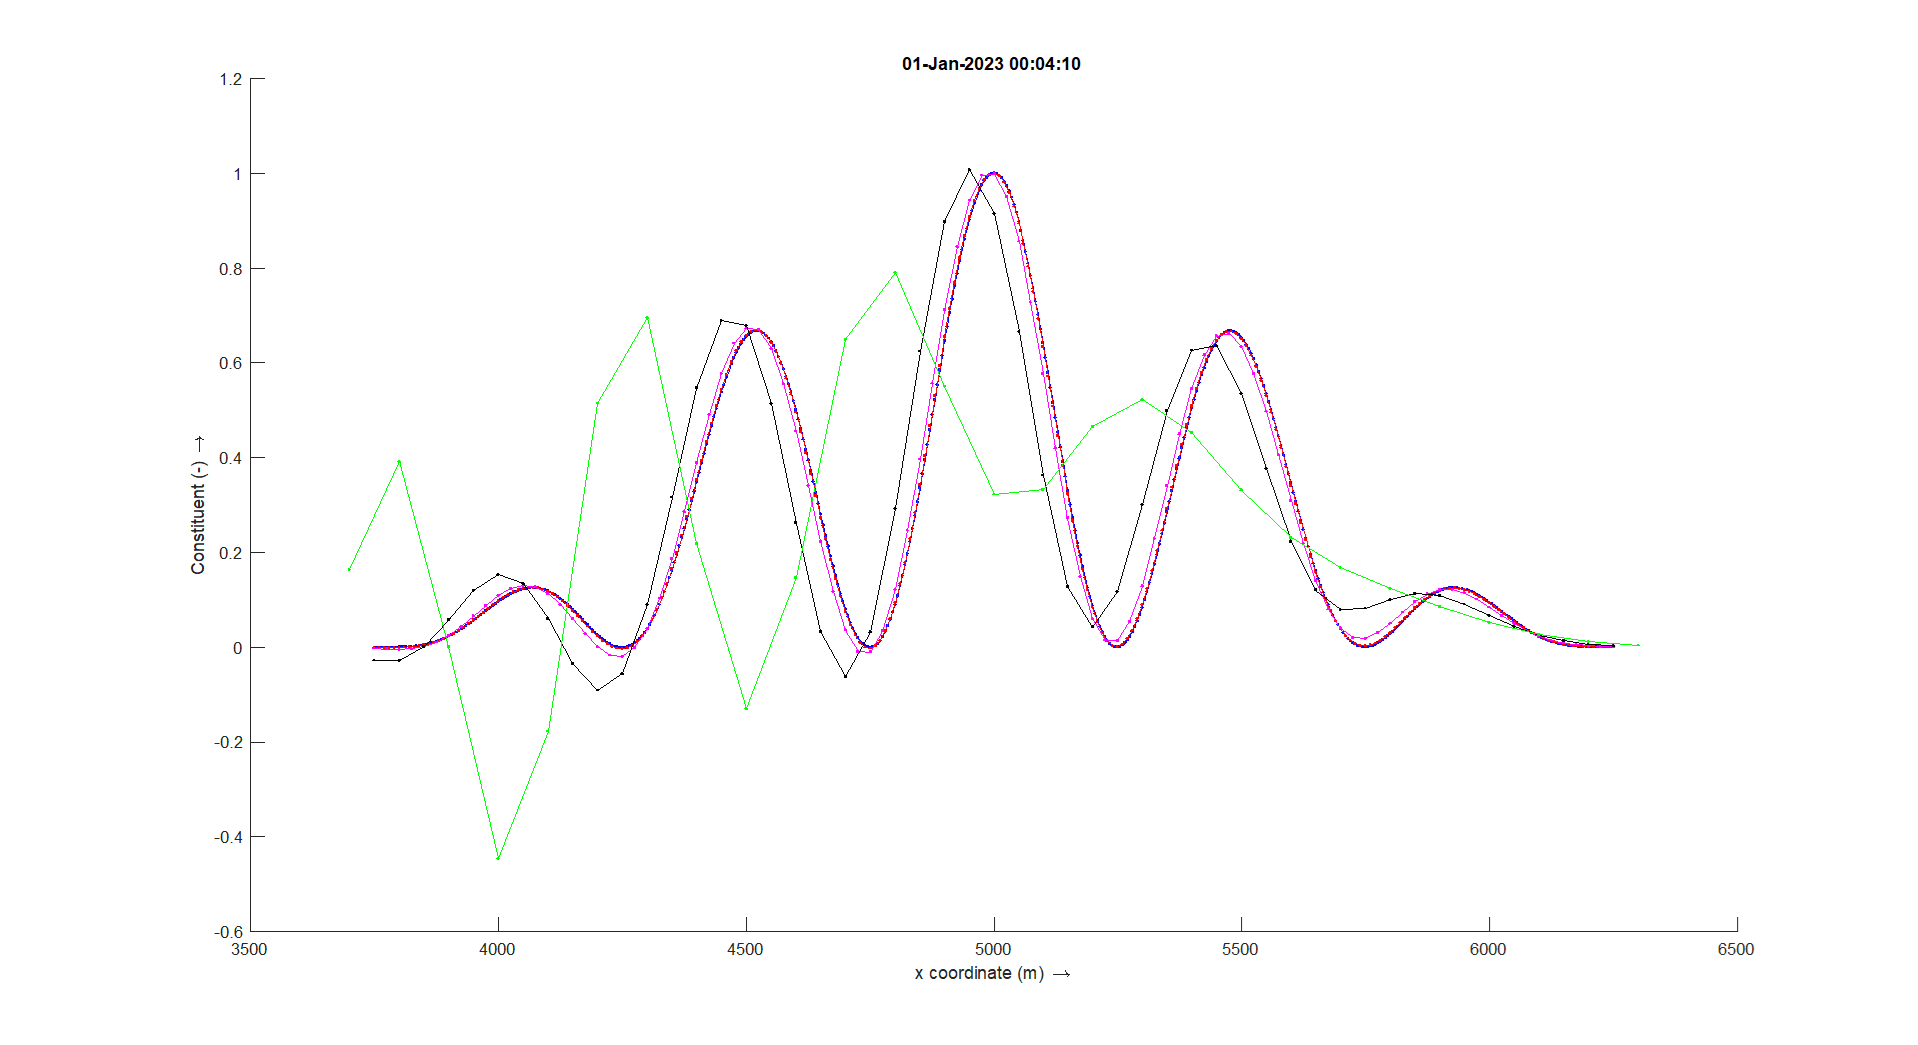
\includegraphics[width=0.9\textwidth]{figures/wave_package_250s.png}
    \caption[Wave package experiment]{Wave package experiment, results at $t=\bqty{250}{\second}$ and $\Dt = \bqty{0.01}{\second}$:
        Blue: $\Dx = \bqty{5}{\metre}$,
        Red: $\Dx = \bqty{10}{\metre}$,
        Cyan: $\Dx = \bqty{25}{\metre}$,
        Black: $\Dx = \bqty{50}{\metre}$,
        Green: $\Dx = \bqty{100}{\metre}$.
    }
    \label{fig:result_wave_package}
\end{figure}


%--------------------------------------------------------------------------------
\subsection{Transport of strictly positive constituent}
When $c$ needs a strickly positive value (like a concentration) then due to numerical discretization the value $c$ could become negative, even if the initial and boundary values are positive.
In certain applications a positive value is required and even small negative are not allowed.
To ensure the positivity of the constituent $c$ we will write the equation with variable $\phi$, where $\phi$ is defined as:
\begin{align}
    c = \exp(\ln(c)) =  \exp(\phi), \quad \text{with} \quad \phi = \ln(c)
\end{align}
The considered advection-diffusion equation than reads:
\begin{align}
    \int_\Omega\pdiff{{e^\phi}}{t} \, d\omega
    + \int_\Omega\pdiff{\left(u{e^\phi}\right)}{x} \, d\omega
    - \int_\Omega\pdiff{}{x}\left(\eps \pdiff{{e^\phi}}{x}\right)\, d\omega = 0,\label{eq:1d_advec_phi_num}
\end{align}
With initial condition for the velocity $u_{\it given} = \bqty{10}{\metre\per\second}$, which coincide with the wave celerity in the next numerical experiments.
\begin{align}
    u(x,0) = u_{\it given}
\end{align}
and with a prescribed boundary condition for the constituent $c$ at the left side of the domain
\begin{align}
    c(0,t) = c_{\it given}
    \begin{cases}
        \half \cos\left(\pi \left(\frac{t_{reg} - t}{t_{reg}}\right)+ 1\right) &\quad \text{if } t < t_{reg},
        \\
        1 &\quad \text{if } t \geq t_{reg},
    \end{cases}
\end{align}
where
\begin{symbollist}
    \item[$t_{reg}$] The regularization time for the given time-series, [\si{\second}]
    \nomenclature{$t_{reg}$}{\si{\second}}{The regularization time for the given time-series}
\end{symbollist}
A value of $c(0,t)=0$ is estimated by:
\begin{align}
    \phi(0,t) = \ln(c(0,t)) \gtrsim -25
\end{align}
%--------------------------------------------------------------------------------
\paragraph*{Numerical experiment}
The numerical experiment is performed with the following parameters:
\begin{itemize}
    \item Length of the domain, $\bqty{12000}{\metre}$
    \item Grid size, $\Dx = \bqty{10}{\metre}$
    \item Start time, $t_{start} = \bqty{0}{\second}$
    \item End time, $t_{stop} = \bqty{3600}{\second}$
    \item Timestep, $\Dt = \bqty{5}{\second}$
    \item Regularization time for time-series, $t_{reg} = \bqty{300}{\second}$
    \item Prescribed constant velocity, $u_{\it given}(x,t) = \bqty{10}{\metre\per\second}$
    \item Prescribed initial value of the constituent, $c(x,0)= \num{1.4e-11}$, \newline so $\phi = \bqty{-25}{-}$.
    \item Prescribed constant constituent on boundary $c_{\it given}(0,t) = 1$, \newline so $\phi = \ln(c_{\it given}(0,t)) = \ln(1) = \bqty{0}{-}$
\end{itemize}
%--------------------------------------------------------------------------------
\paragraph*{Results of the numerical experiments}
\notyet
%--------------------------------------------------------------------------------
\section{1-D Advection-diffusion equation}
In this section we will show the resuls of the advection-diffusion equation with a Dirichlet boundary conditions at both sides of the domain and an interface problem, i.e.\ a large jump of the diffusion coefficiebt in the middle of the domain.

The considered advection-diffusion equation reads:
\begin{align}
    \pdiff{c}{t} + \pdiff{uc}{x} - \pdiff{}{x}\left( (\eps+\Psi) \pdiff{c}{x}\right)= 0, \qquad u>0. \label{eq:1d_advection_art_diff}
\end{align}
where
\begin{symbollist}
    \item[$c$] Constituent, $\bunit{-}$.
    \item[$u$] Advection velocity, $\bunit{\metre\per\second}$.
    \item[$\eps$] Diffusion coefficient, $\bunit{\square\metre\per\second}$.
    \item[$\Psi$] Artificial diffusion, $\bunit{\square\metre\per\second}$.
\end{symbollist}

%--------------------------------------------------------------------------------
\subsection{Outflow boundary layer}\label{sec:1d_numerical_outflow_boundary_layer_experiment}
The Dirichlet value at the outflow boundary is so chosen that there will appear an outflow boundary layer.
Due to this outflow boundary the numerical scheme need to have a cell P\'eclet number ($\Pe = u\Dx/\eps$) smaller then two in the vicinity of that layer.
In the \deltaformulation that will be reach by a regularization step, i.e. increase the diffusion in the vicinity of the boundary layer.
To force a outflow boundary layer at both boundaries a Dirichlet boundary is prescribed.
With the boundary conditions
$c(0,t) = a$ and $c(L,t) = b$ the analytic solution read:
\begin{align}
    c(x) = a + (b-a) \frac{e^{\frac{(x-L)}{L}\Pe} -  e^{-\Pe}}{1 - e^{-\Pe}},
\end{align}
with $\Pe = u L/\eps$.

%--------------------------------------------------------------------------------
\paragraph*{Numerical experiment}
The numerical experiment is performed with the following parameters:
\begin{itemize}
    \item Length of the domain $L_x = \bqty{1000}{\metre}$.
    \item Stationary simulation, $\lpdiff{c}{t}=0$.
    \item Prescribed boundary conditions: $c(0,t) = 0$ and $c(L_x,t) = 1$.
    \item Grid size $\Dx = \bqty{10}{\metre}$,
    \item Diffusion coefficient $\eps = \bqty{10}{\square\metre\per\second}$
    \item Advection velocities, $\Pe = u\Dx/\eps$:
    \begin{itemize}
        \item $u = \bqty{1}{\metre\per\second} \rightarrow \Pe = 1.0$
        \item $u = \bqty{1.9}{\metre\per\second} \rightarrow \Pe = 1.9$
        \item $u = \bqty{2.1}{\metre\per\second} \rightarrow \Pe = 2.1$
        \item $u = \bqty{5.0}{\metre\per\second} \rightarrow \Pe = 5.0$
    \end{itemize}
    \item Smoothing factor, $c_{\Psi} = 4$
    \item Right hand side to compute artificial viscosity, $\frac{1}{32} c_{\Psi} u \Dx \lpdiff[2]{c}{\xi}$ (educational guess).
\end{itemize}
%--------------------------------------------------------------------------------
\paragraph*{Results of the numerical experiments}
Map results are presented for the constituent $c$ and the artificial diffusion $\Psi$.
\begin{figure}[H]
    \begin{subfigure}{0.5\textwidth}
    \centering
    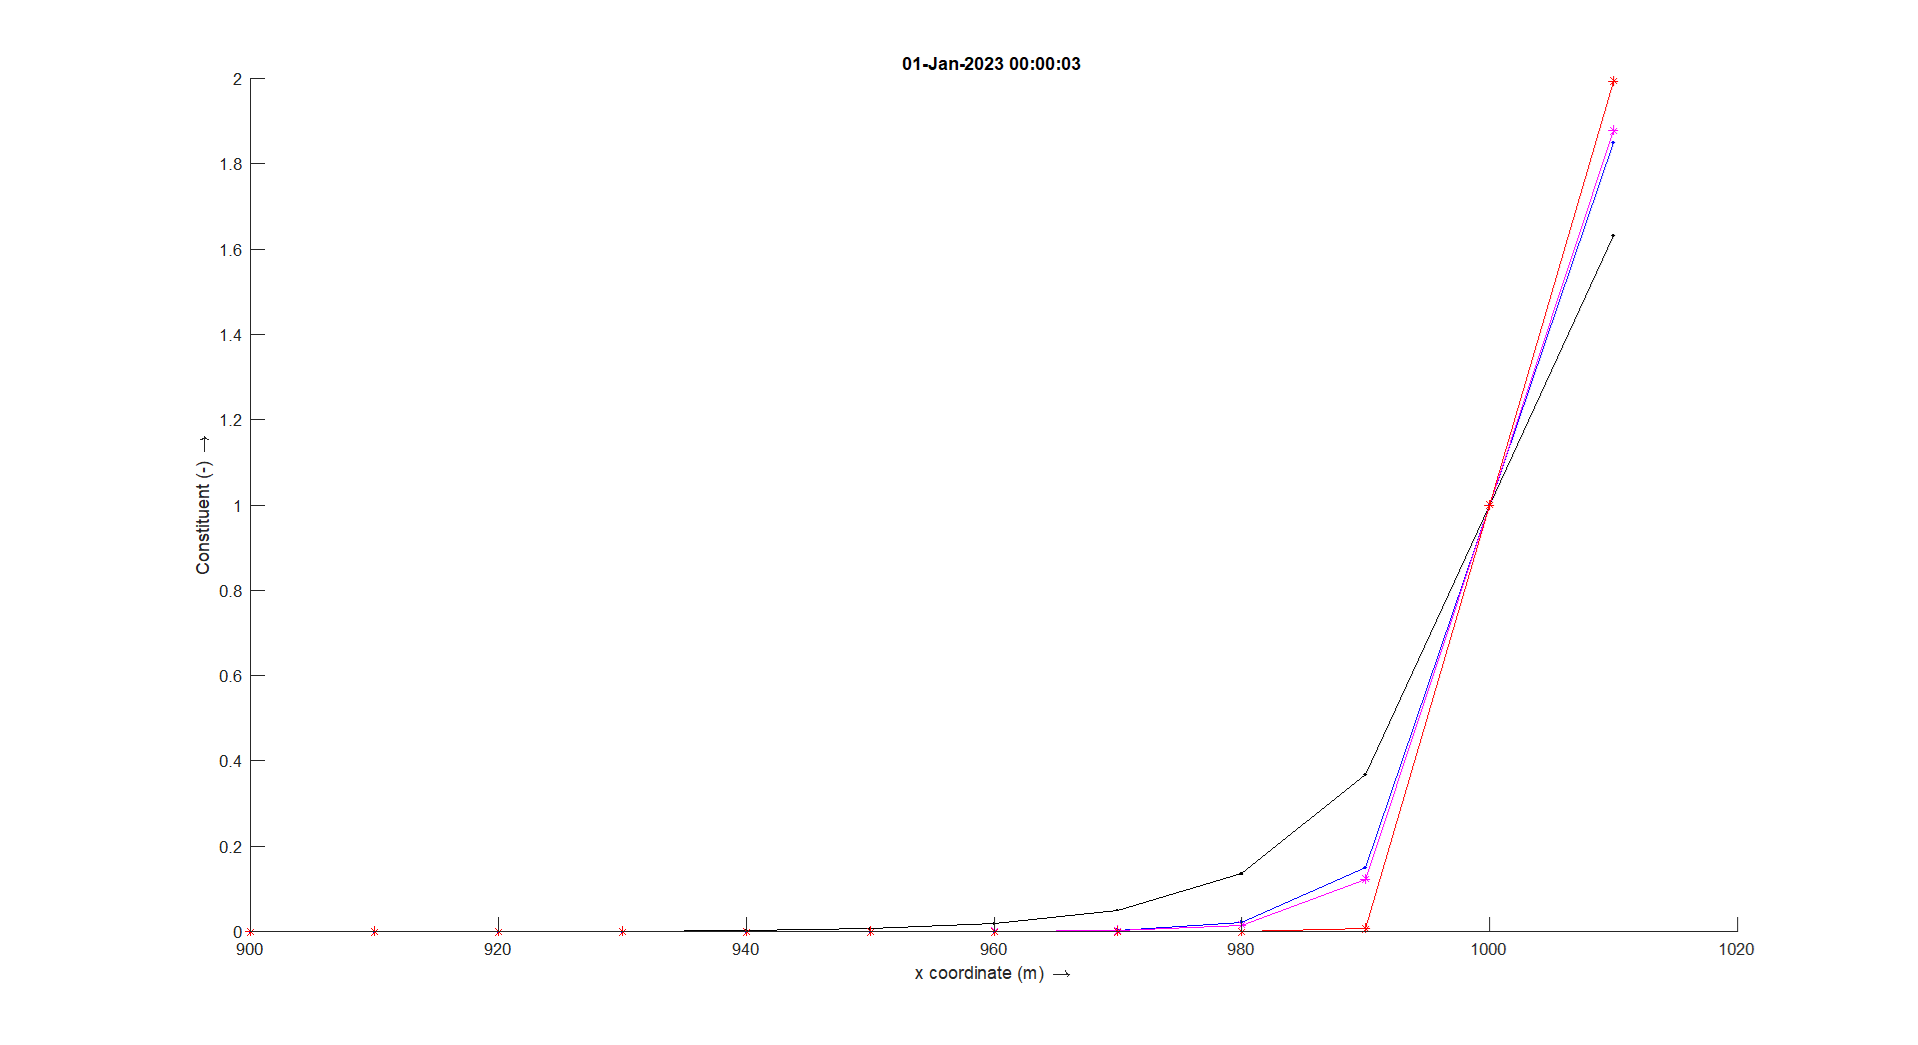
\includegraphics[width=0.9\textwidth]{figures/analytic_boundary_layer.png}
    \caption{Analytic solution}
    \end{subfigure}
    \begin{subfigure}{0.5\textwidth}
    \centering
    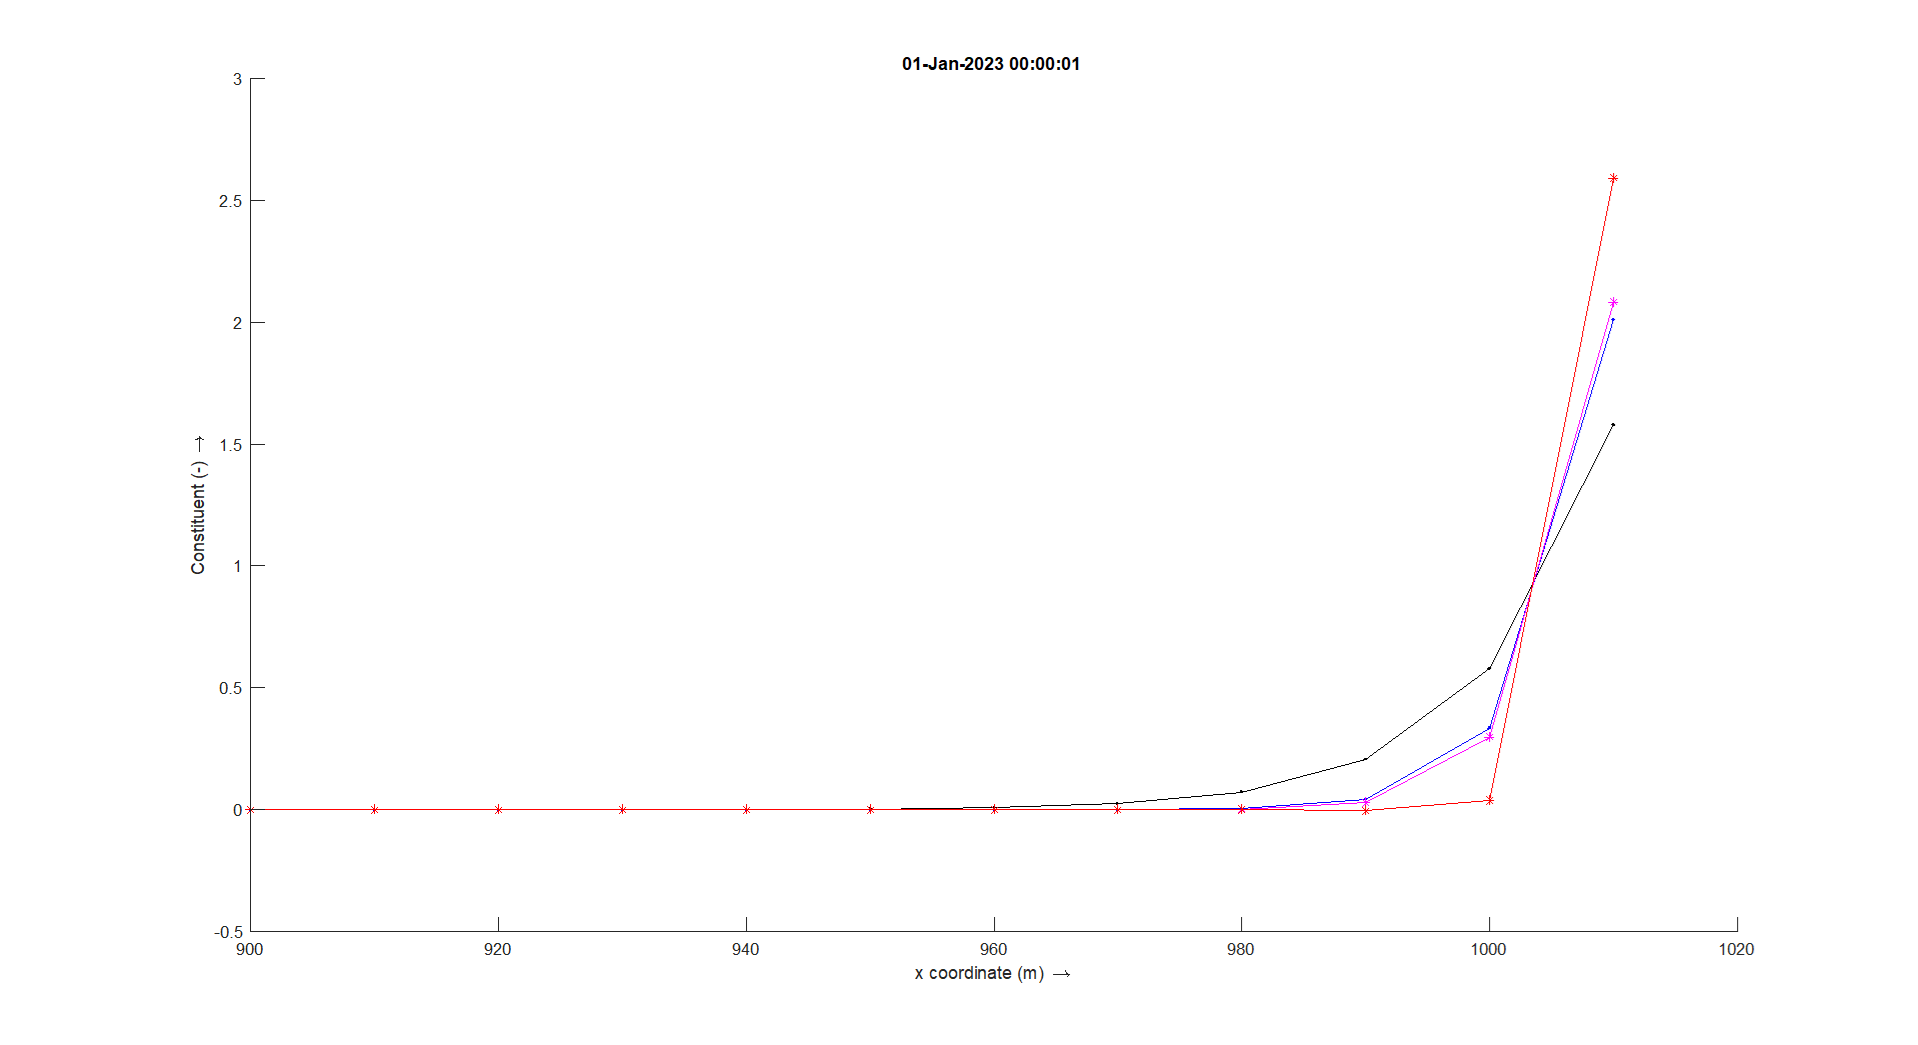
\includegraphics[width=0.9\textwidth]{figures/adv_diff_constituent.png}
    \caption{Numerical solution}
    \end{subfigure}
    \caption{Map results for different values of the advection velocity (thus P\'eclet number). The graphs with an  asterix represent results with a cell P\'eclet number larger then two. Black: $\Pe = 1.0$; Blue: $\Pe = 1.9$, Green: $\Pe = 2.1$; Cyan: $\Pe = 5.0$.}
\end{figure}
\begin{figure}[H]
    \centering
    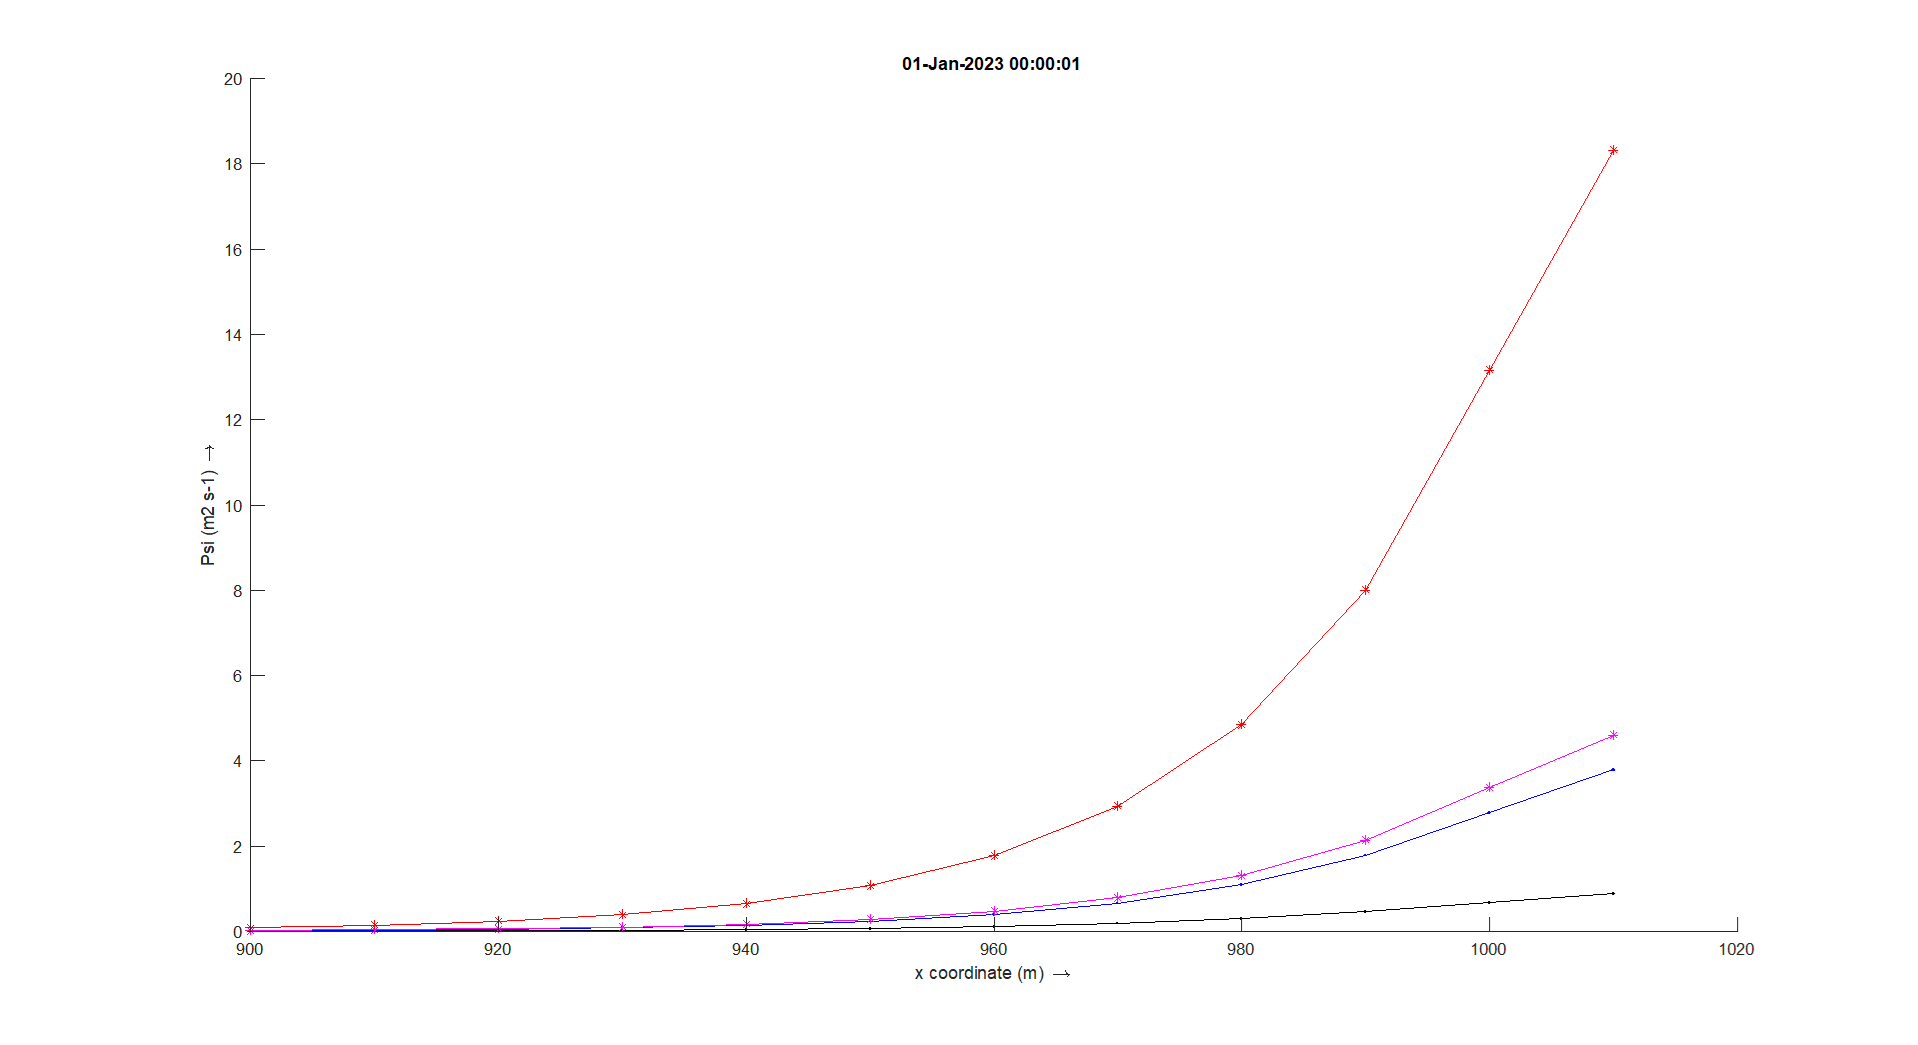
\includegraphics[width=0.9\textwidth]{figures/adv_diff_psi.png}
\caption{Map results for the used artificial diffusion $\Psi$. Black: $\Pe = 1.0$; Blue: $\Pe = 1.9$, Green: $\Pe = 2.1$; Cyan: $\Pe = 5.0$.}
\end{figure}
\begin{figure}[H]
    \centering
    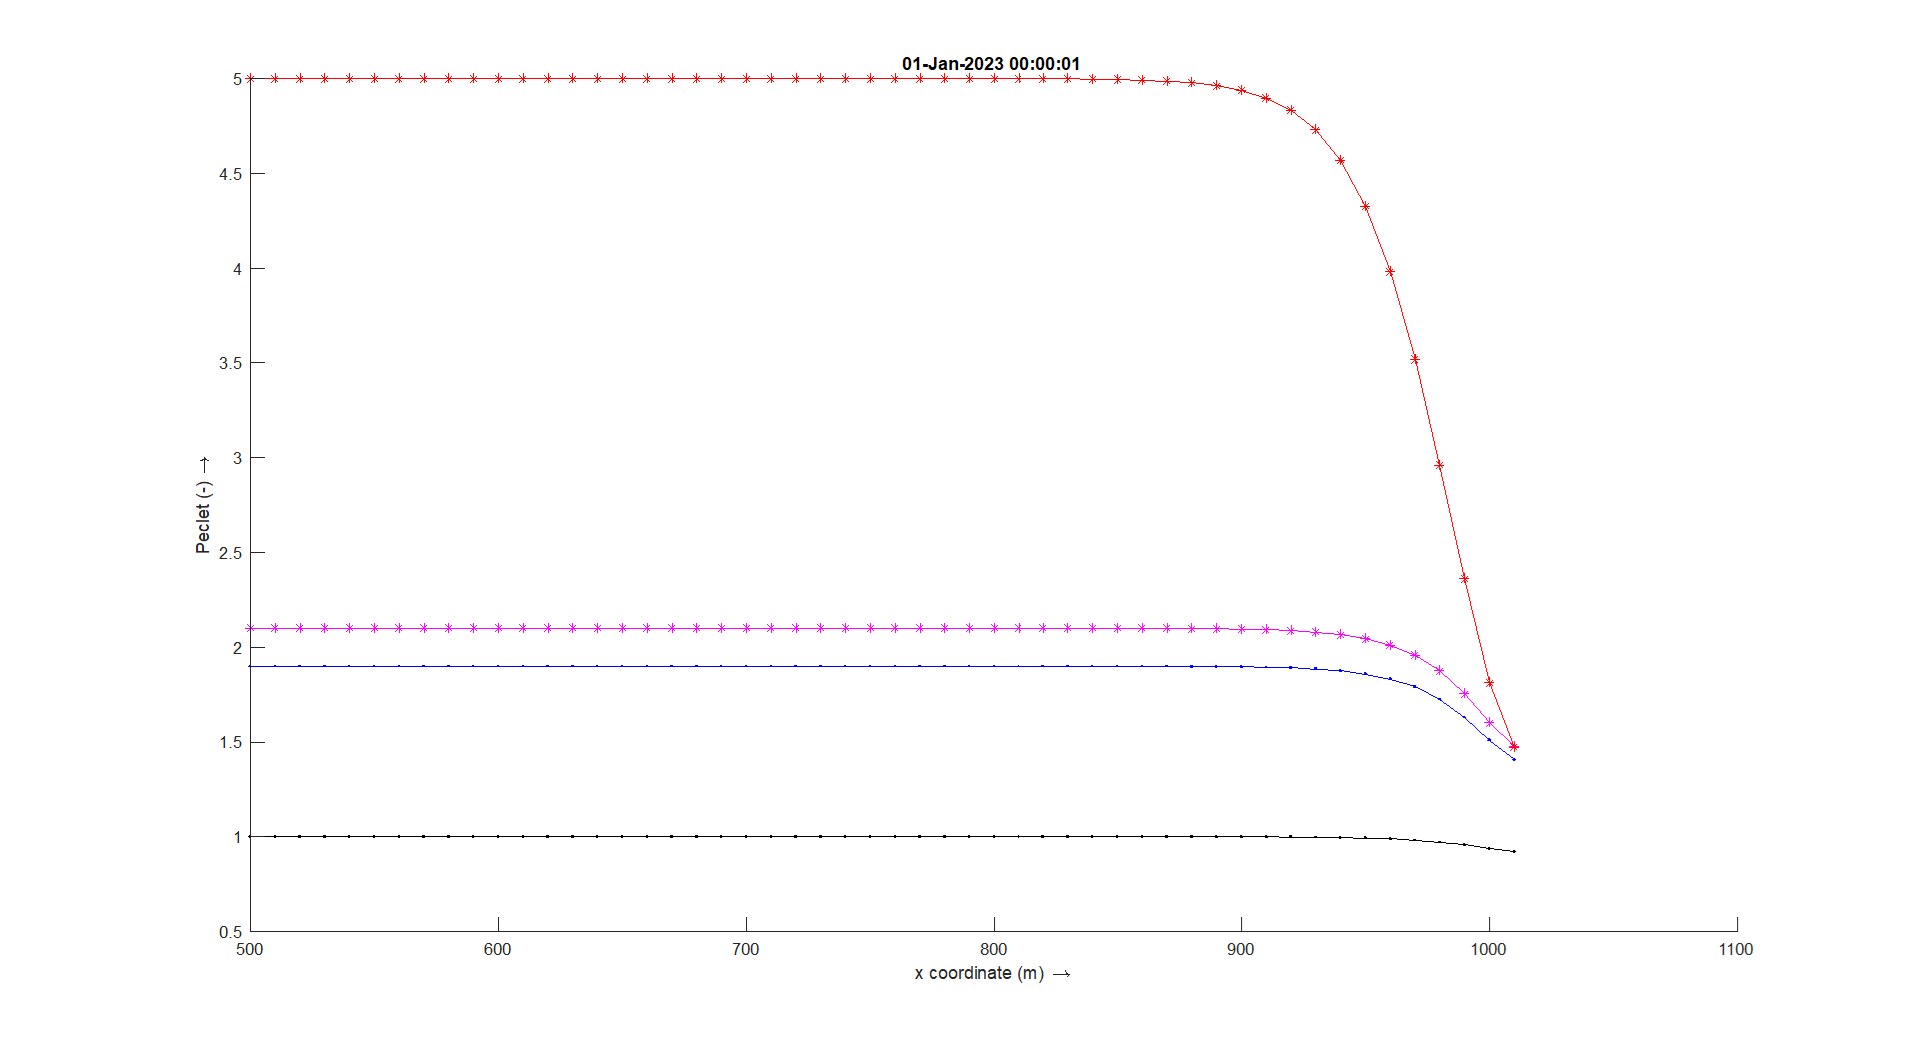
\includegraphics[width=0.9\textwidth]{figures/adv_diff_peclet.png}
    \caption{Map results for the used cell P\'eclet number. Black: $\Pe = 1.0$; Blue: $\Pe = 1.9$, Green: $\Pe = 2.1$; Cyan: $\Pe = 5.0$.}
\end{figure}

%--------------------------------------------------------------------------------
\subsection{Interface problem}\label{sec:1d_numerical_interface_experiment}
A numerical experiments is performed for the stationary advection-diffusion equation with a jump in the diffusion coefficient as described by:
\begin{align}
    \eps(x) &=
    \begin{cases}
        \check{\eps}, & \quad \text{if} \quad 0 < x \leq x^*, \\
        1, & \quad \text{if} \quad x^* < x < 1
    \end{cases}
\end{align}
An analytical solution exists in case $u=0$ and read \citep[eq.\ 3.11]{Wesseling2001}:
\begin{align}
    c(x)& =
    \begin{cases}
        \alpha x, & \quad \text{if} \quad 0 < x \leq x^*, \\
        \check{\eps}\alpha x + 1 - \check{\eps}\alpha, & \quad \text{if} \quad x^*<x<1
    \end{cases} \\
    \alpha & = \frac{1}{x^* -\check{\eps} x^* + \check{\eps}}
\end{align}

\begin{itemize}
    \item If $\eps \pdiff{c}{x} \equiv 0$ then either $\eps=0$ or $\pdiff{c}{x}=0$. Where $\eps=0$ is not feasible.
\end{itemize}

Some numerical experiments are performed with several values of $u$.

%--------------------------------------------------------------------------------
\paragraph*{Numerical experiment}
The numerical experiment is performed with the following parameters:
\begin{itemize}
    \item Length of the domain $L_x = \bqty{1}{\metre}$.
    \item Stationary simulation, $\lpdiff{c}{t}=0$.
    \item Prescribed boundary conditions: $c(0,t) = 0$ and $c(L_x,t) = 1$.
    \item Grid size: %  , $u = \bqty{0.9}{\metre\per\second}$
    \begin{itemize}
        \item $\Dx = \bqty{0.001}{\metre} \rightarrow \Pe = 0.09$,
        \item $\Dx = \bqty{0.01}{\metre} \rightarrow \Pe = 0.9$,
        \item $\Dx = \bqty{0.05}{\metre} \rightarrow \Pe = 4.5$,
    \end{itemize}
    \item Diffusion coefficient $\check{\eps} = \bqty{0.01}{\square\metre\per\second}$
    \item Advection velocities, $\Pe = u\Dx/\eps$:
    \begin{itemize}
        \item $u = \bqty{0}{\metre\per\second} \rightarrow \Pe = 0.0$
        \item $u = \bqty{0.9}{\metre\per\second} \rightarrow \Pe = 0.09, \Pe = 0.9\text{ and } \Pe = 4.5$
    \end{itemize}
\end{itemize}
%--------------------------------------------------------------------------------
\paragraph*{Results of numerical experiment}
Map results are presented for the constituent $c$ and the artificial diffusion $\Psi$.
\begin{figure}[H]
    \begin{subfigure}[t]{0.5\textwidth}
        \centering
        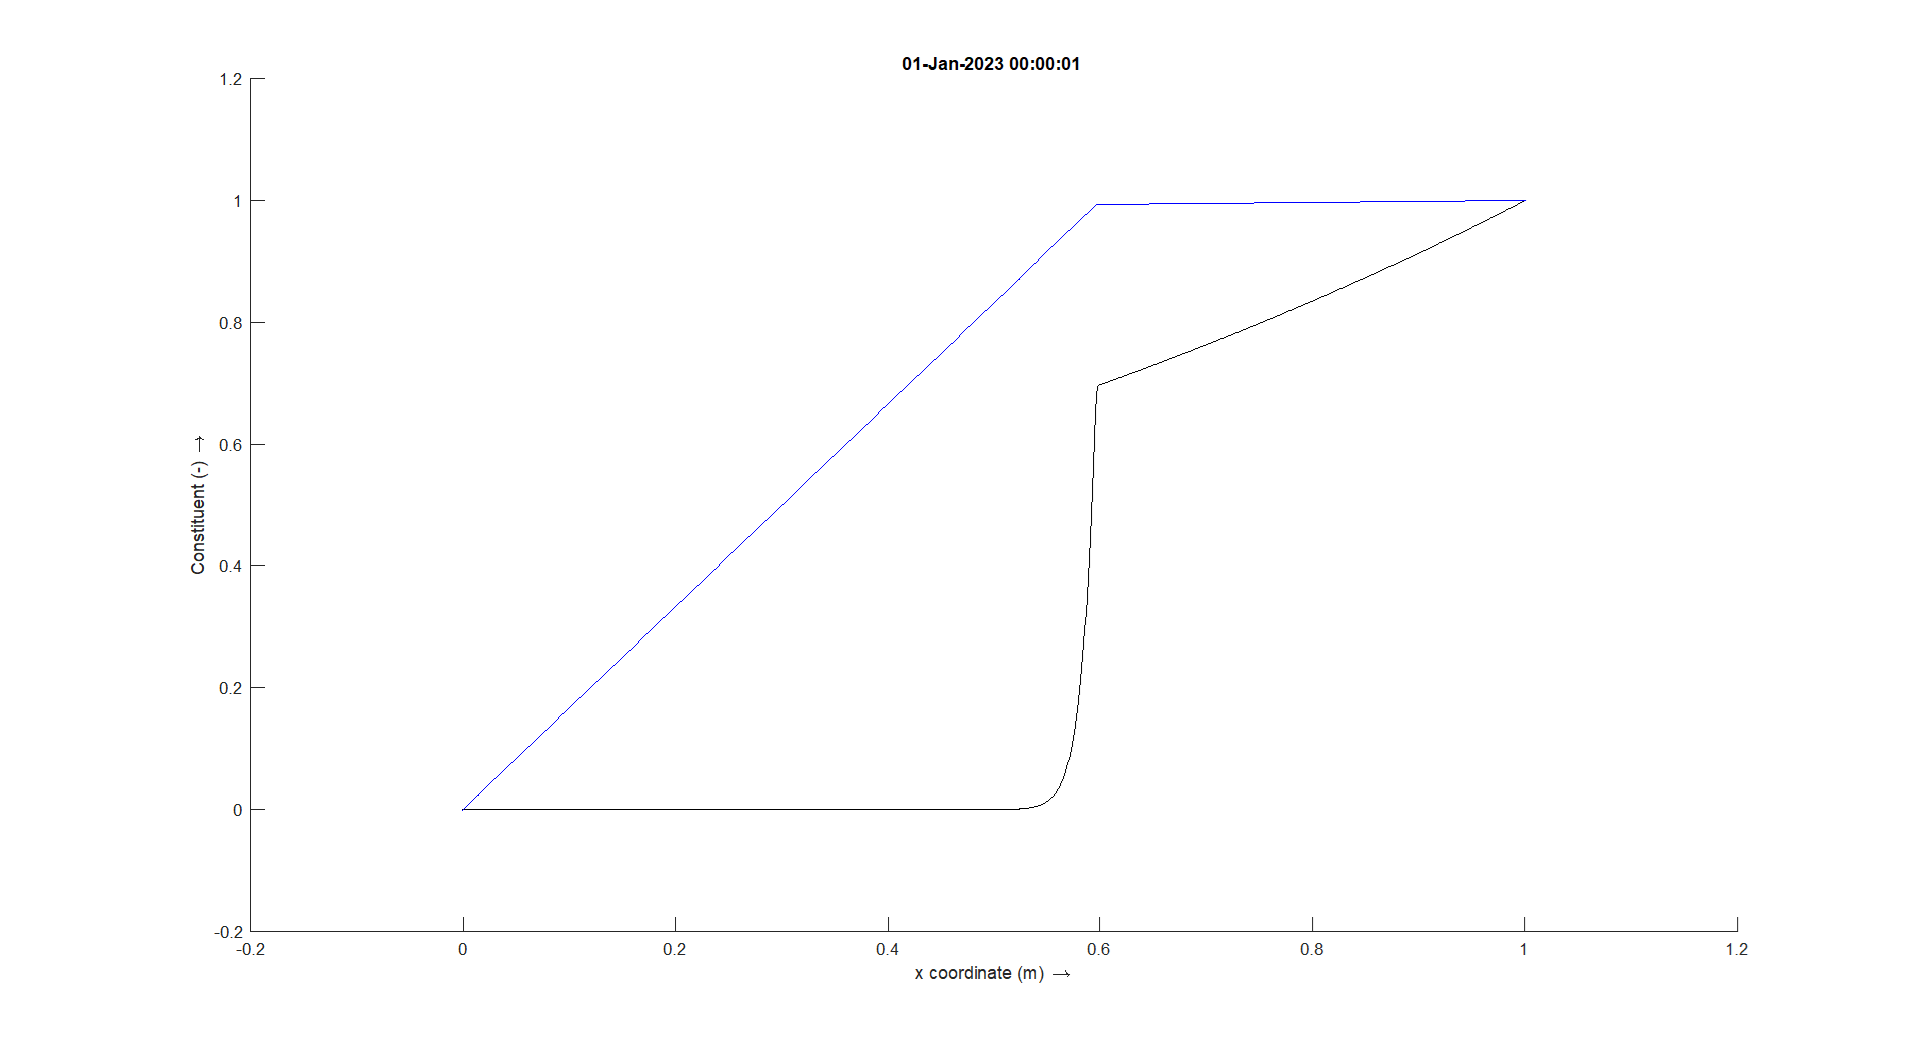
\includegraphics[width=0.9\textwidth]{figures/interface_u0d0_u0d9.png}
        \caption{High numerical resolution solution $\Dx=\bqty{0.001}{\metre}$.  Blue: $u =\bqty{0}{\metre\per\second}$ and Black: $u = \bqty{0.9}{\metre\per\second}$.}
    \end{subfigure}
    \hfill
    \begin{subfigure}[t]{0.5\textwidth}
        \centering
        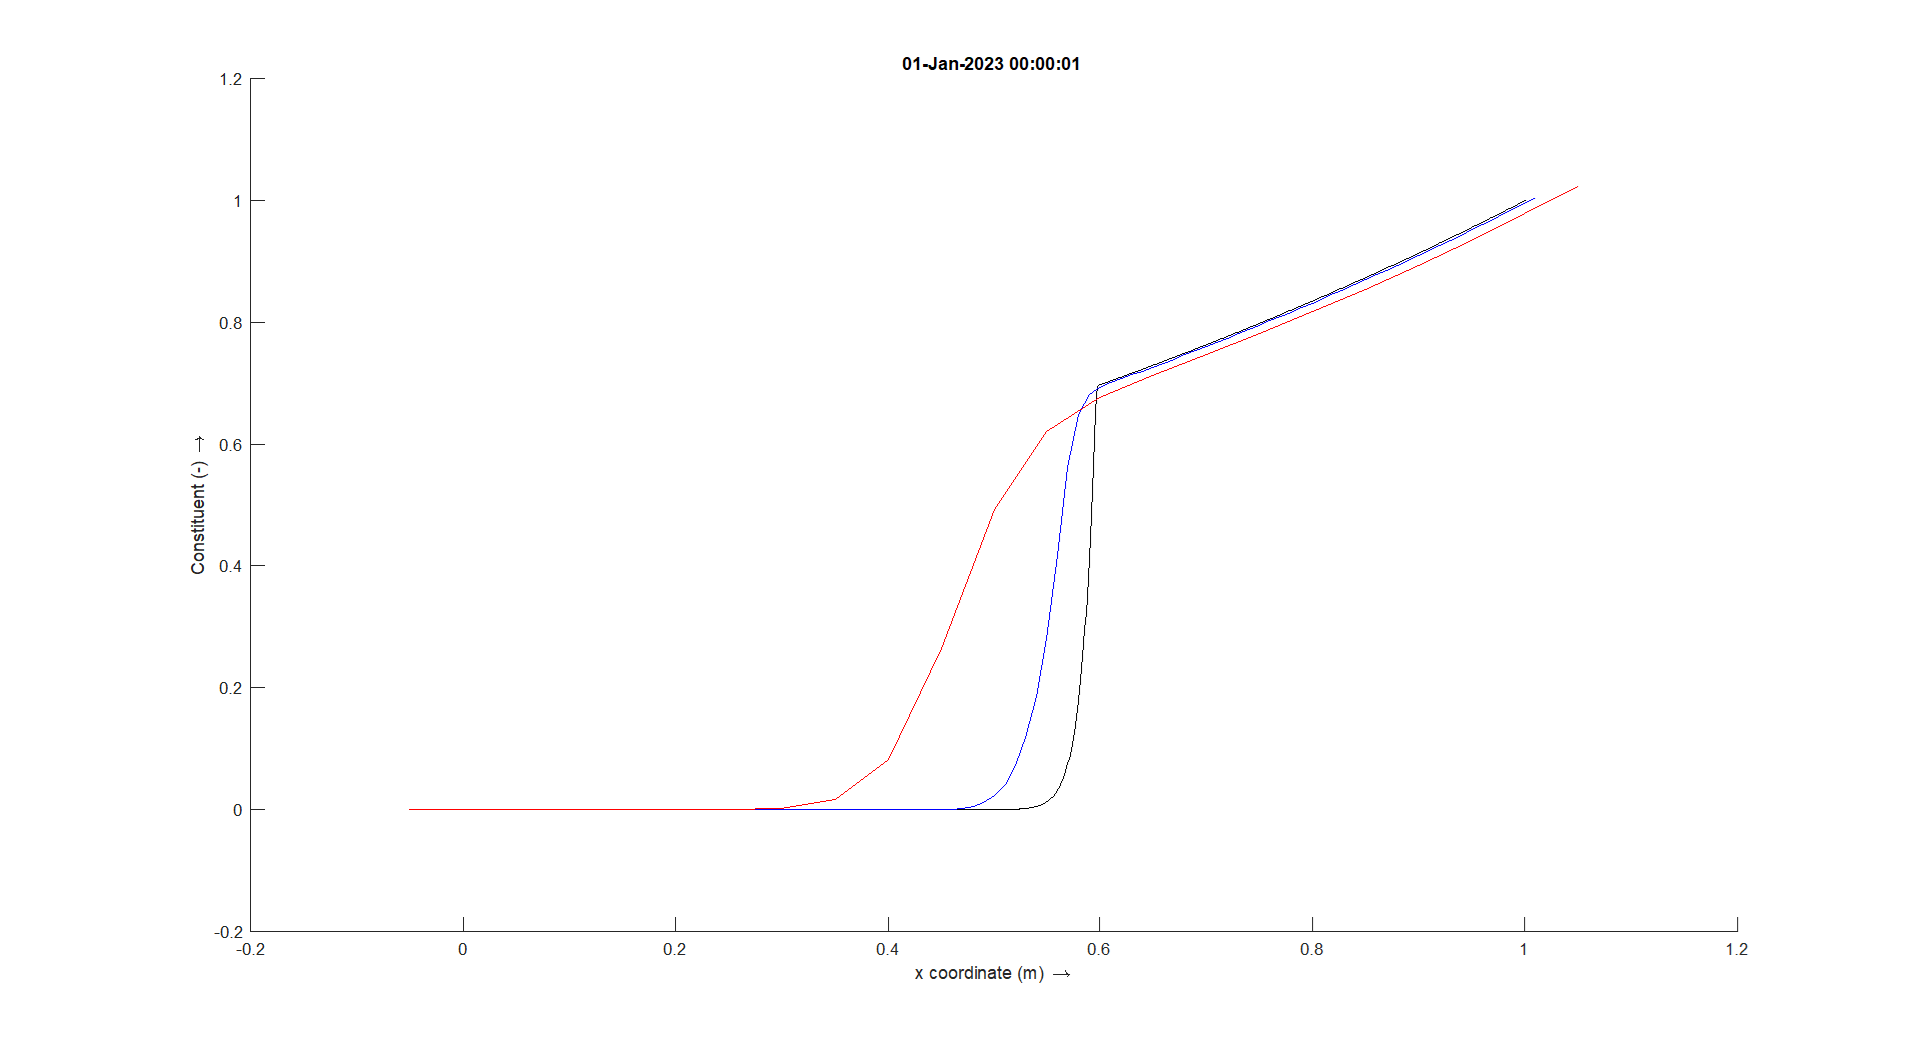
\includegraphics[width=0.9\textwidth]{figures/interface_pe0d09_pe0d9_pe4d5.png}
        \caption{Numerical solution, $u = \bqty{0.9}{\metre\per\second}$. Black: $\Dx = \bqty{0.001}{\metre} \rightarrow \Pe= 0.09$; Blue: $\Dx = \bqty{0.01}{\metre} \rightarrow \Pe = 0.9$ and Red: $\Dx = \bqty{0.05}{\metre} \rightarrow \Pe = 4.5$.}
    \end{subfigure}
    \caption{Map results for different values of the P\'eclet number.}
\end{figure}
%--------------------------------------------------------------------------------
\section{1-D Wave equation}
%--------------------------------------------------------------------------------
\subsection{Gaussian hump}\label{sec:numerical_experiment}
The considered 1-D wave equation reads:
\begin{align}
    \pdiff{h}{t}  + \pdiff{q}{x} & = 0 \qquad \textit{continuity eq.} \\
    \pdiff{q}{t}  + g h \pdiff{h}{x} & = 0 \qquad \textit{momentum eq.}
\end{align}
%
With initial conditions
\begin{align}
    h(x,0) & = \zeta(x,0) - z_b(x), \quad \bunit{\metre} \\
    q(x,0) & = 0, \quad \bunit{\square\metre\per\second}
\end{align}
for the the water level a Gaussian hump is prescribed
\begin{align}
    \zeta(x) = 2 a_0 \exp\left( - \frac{(x - \mu)^2}{2\sigma^2}  \right), \quad \bunit{\metre}
\end{align}
At the boundaries no ingoing signals are prescribed, so outgoing signals are leaving the domain unhampered, which means no reflections will be present other then numerical reflections.
%--------------------------------------------------------------------------------
\paragraph*{Numerical experiment}
The numerical experiment is performed with the following parameters:
\begin{itemize}
    \item Length of the domain, $L_x = \bqty{12000}{\metre}$, ranging from $\bqty{-6000}{\metre}$ to $\bqty{6000}{\metre}$.
    \item Bed level, $z_b = \bqty{-10}{\metre}$.
    \item Grid size, $\Dx = \bqty{10}{\metre}$.
    \item Start time, $t_{start} = \bqty{0}{\second}$.
    \item End time, $t_{stop} = \bqty{3600}{\second}$.
    \item Timestep, $\Dt = \bqty{10}{\second}$.
    \item Regularization time for time-series, $t_{reg} = \bqty{300}{\second}$.
    \item Amplitude of the Gaussian hump at the boundary, $a_0 = \bqty{0.01}{\metre}$.
    \item Centre of the Gaussian hump, $\mu = \bqty{3000}{\metre}$.
    \item Spreading of the Gaussian hump, $\sigma = \bqty{700}{\metre}$.
\end{itemize}
And a second experiment with given boundary values:
\begin{itemize}
    \item Prescribed discharge boundary at $\bqty{-6000}{\metre}$: $q(0,t) = \bqty{0.05}{\square\metre\per\second}$.
    \item Prescribed water level boundary value at $\bqty{6000}{\metre}$: $\zeta(0,t) = \bqty{0.02}{\metre}$.
\end{itemize}
Because the boundary values are constant in time the solution is time-independent.
Therefore two simulation should be performed:
\begin{enumerate}
    \item A stationary computation (with $\Dt = \bqty{0}{\second}$) and
    \item an temporal computation (with $t_{stop} = \bqty{10800}{\second}$)
\end{enumerate}
%--------------------------------------------------------------------------------
\paragraph*{Results of the numerical experiments 1}
\notyet
%--------------------------------------------------------------------------------
\paragraph*{Results of the numerical experiments 2}
\notyet
%--------------------------------------------------------------------------------
\subsection{Weir}\label{sec:numerical_experiment_weir}
The model is taken from \citet{Borsboom2001}.
The considered 1-D wave equation reads:
\begin{align}
    \pdiff{h}{t} & + \pdiff{q}{x}  = 0, \qquad \textit{continuity eq.} \\
    \pdiff{q}{t} & + \pdiff{(q^2/h)}{x} + g h \pdiff{h}{x} - \pdiff{}{x} \left( (\nu+\Psi) h \pdiff{(q/h)}{x} \right) = 0, \qquad \textit{momentum eq.}
\end{align}
\begin{itemize}
    \item Length of the domain, $\bqty{500}{\metre}$.
    \item Artificial viscosity $\Psi$ computated as presented in \autoref{sec:regularization_artificial_viscosity}.
\end{itemize}
Bathymetry \bunit{\metre}:
\begin{align}
    z_b(x) =
    \begin{cases}
        \num{-12} & 0 < x \leq 200,
        \\
        \num{-12} + 7 (x - 200)/50 & 200 < x \leq 250,
        \\
        \num{-5} & 250 < x \leq 350,
        \\
        \num{-5} - 5(x - 350)/100 & 350 < x \leq 450,
        \\
        \num{-10} & 450 < x \leq 500.
    \end{cases}
\end{align}
Initial conditions
\begin{align}
    h(x,0) & = 0,\\
    q(x,0) & = 0
\end{align}
Boundary conditions
\begin{itemize}
    \item Prescribed discharge boundary at $\bqty{0}{\metre}$: $q(0,t) = \bqty{19.8656}{\square\metre\per\second}$.
    \item Prescribed water level boundary value at $\bqty{500}{\metre}$: $\zeta(500,t) = \bqty{-3}{\metre}$.
\end{itemize}
%--------------------------------------------------------------------------------
\paragraph*{Numerical experiment}
The numerical experiment is performed with the following parameters:
\begin{itemize}
    \item Grid size and time step,
    \begin{itemize}
        \item $\Dx = \bqty{10}{\metre}$ and $\Dt = \bqty{2}{s}$
        \item $\Dx = \bqty{5}{\metre}$ and $\Dt = \bqty{1}{s}$
        \item $\Dx = \bqty{2.5}{\metre}$ and $\Dt = \bqty{0.5}{s}$
        \item $\Dx = \bqty{1.25}{\metre}$ and $\Dt = \bqty{0.25}{s}$
    \end{itemize}
    \item Start time, $t_{start} = \bqty{0}{\second}$.
    \item End time, $t_{stop} = \bqty{7200}{\second}$.
    \item Regularization time for time-series, $t_{reg} = \bqty{300}{\second}$.
    \item Kinematic viscosity, $\nu = \bqty{0.01}{\square\metre\per\second}$
    \item $\eps_{bc} = \num{1e-02}$
\end{itemize}
%--------------------------------------------------------------------------------
\paragraph*{Results of the numerical experiments}
Results for the four different computations are shown in \autoref{fig:result_wl_weir}
\begin{figure}[H]
    \centering
    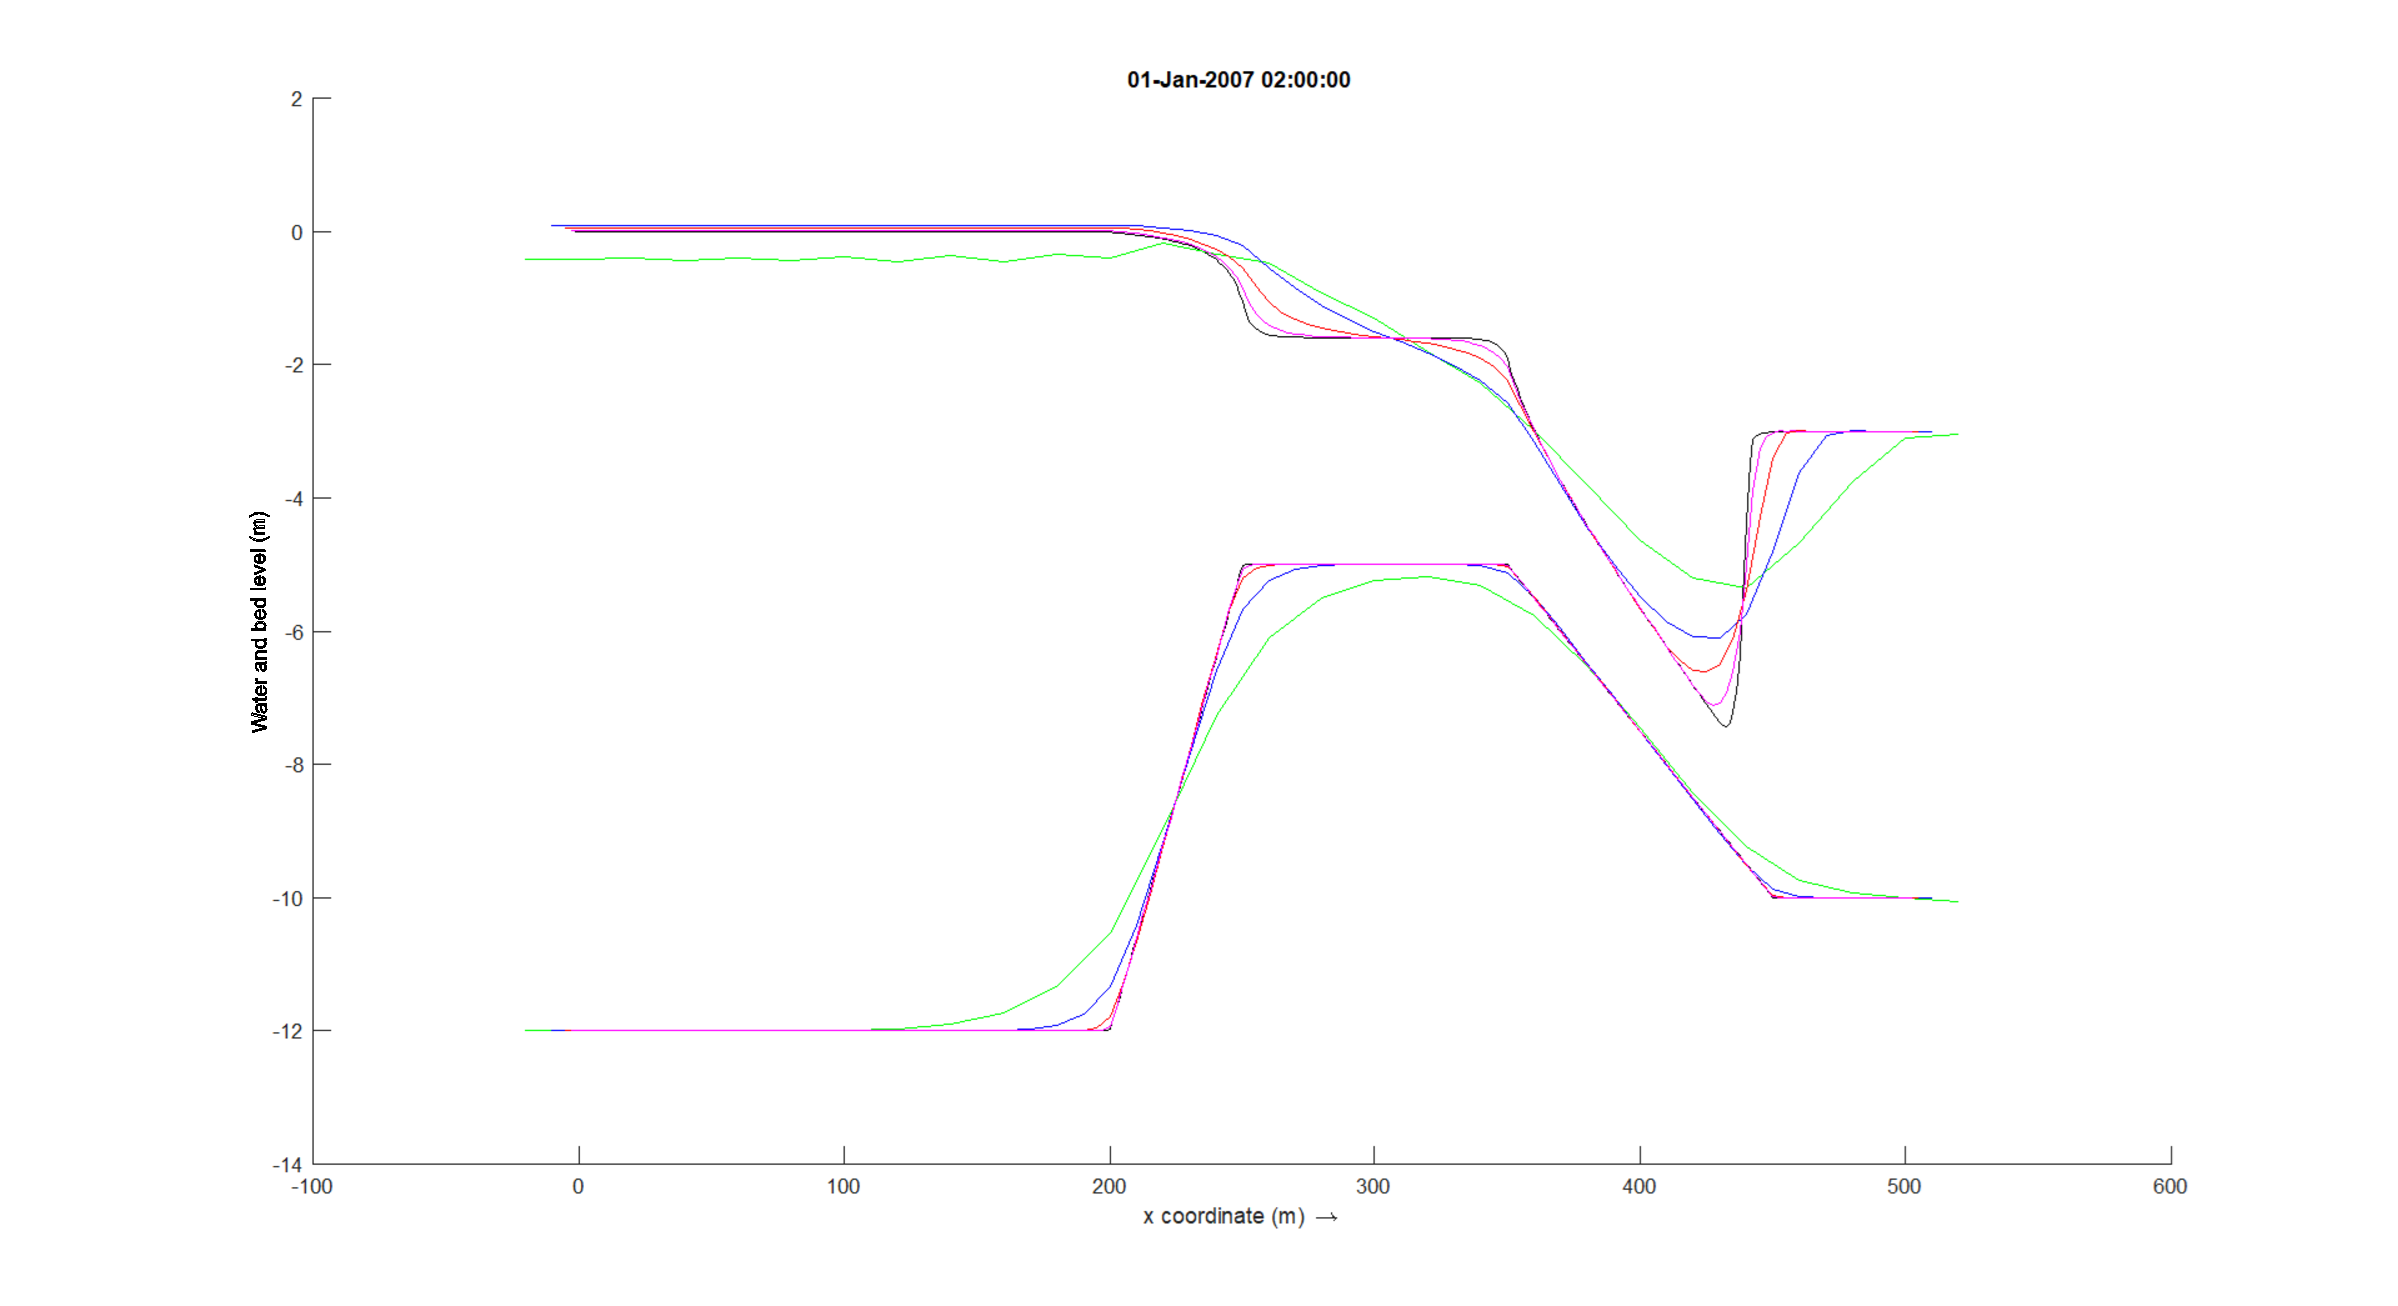
\includegraphics[width=0.9\textwidth]{figures/weir_bed_water_level.pdf}
    \caption[Weir experiment: water level and bed level]{Top graphs present the water level. Lower graphs present the regularized bathymetry.
    Green: $\Dx = \bqty{20}{\metre}$, $\Dt = \bqty{4}{\second}$;
    Blue: $\Dx = \bqty{10}{\metre}$, $\Dt = \bqty{2}{\second}$;
    Red: $\Dx = \bqty{5}{\metre}$, $\Dt = \bqty{1}{\second}$;
    Cyan: $\Dx = \bqty{2.5}{\metre}$, $\Dt = \bqty{0.5}{\second}$;
    Black: $\Dx = \bqty{1.25}{\metre}$, $\Dt =\bqty{0.25}{\second}$
    }
    \label{fig:result_wl_weir}
\end{figure}
%
\begin{figure}[H]
    \begin{subfigure}{0.5\textwidth}
        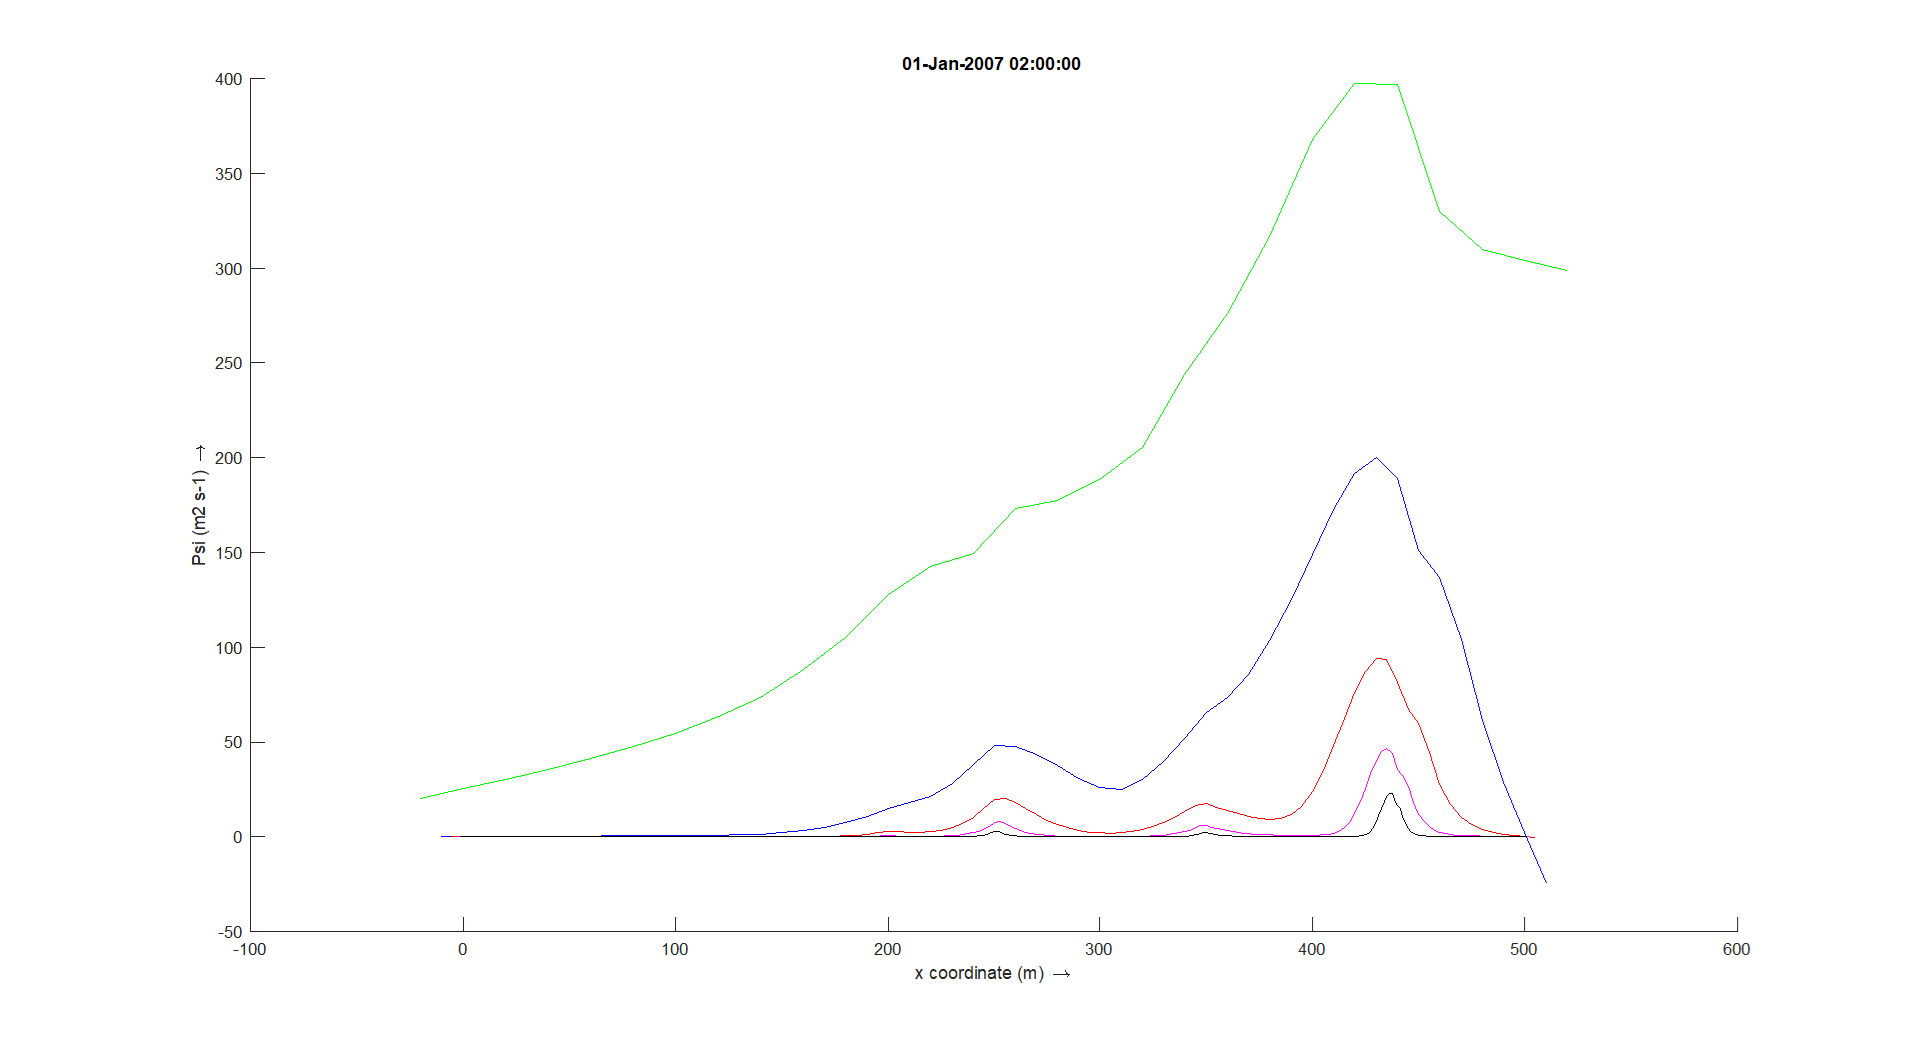
\includegraphics[width=\textwidth]{figures/weir_psi.png}
        \caption{Artificial viscosity $\Psi$.}
    \end{subfigure}
    \begin{subfigure}{0.5\textwidth}
        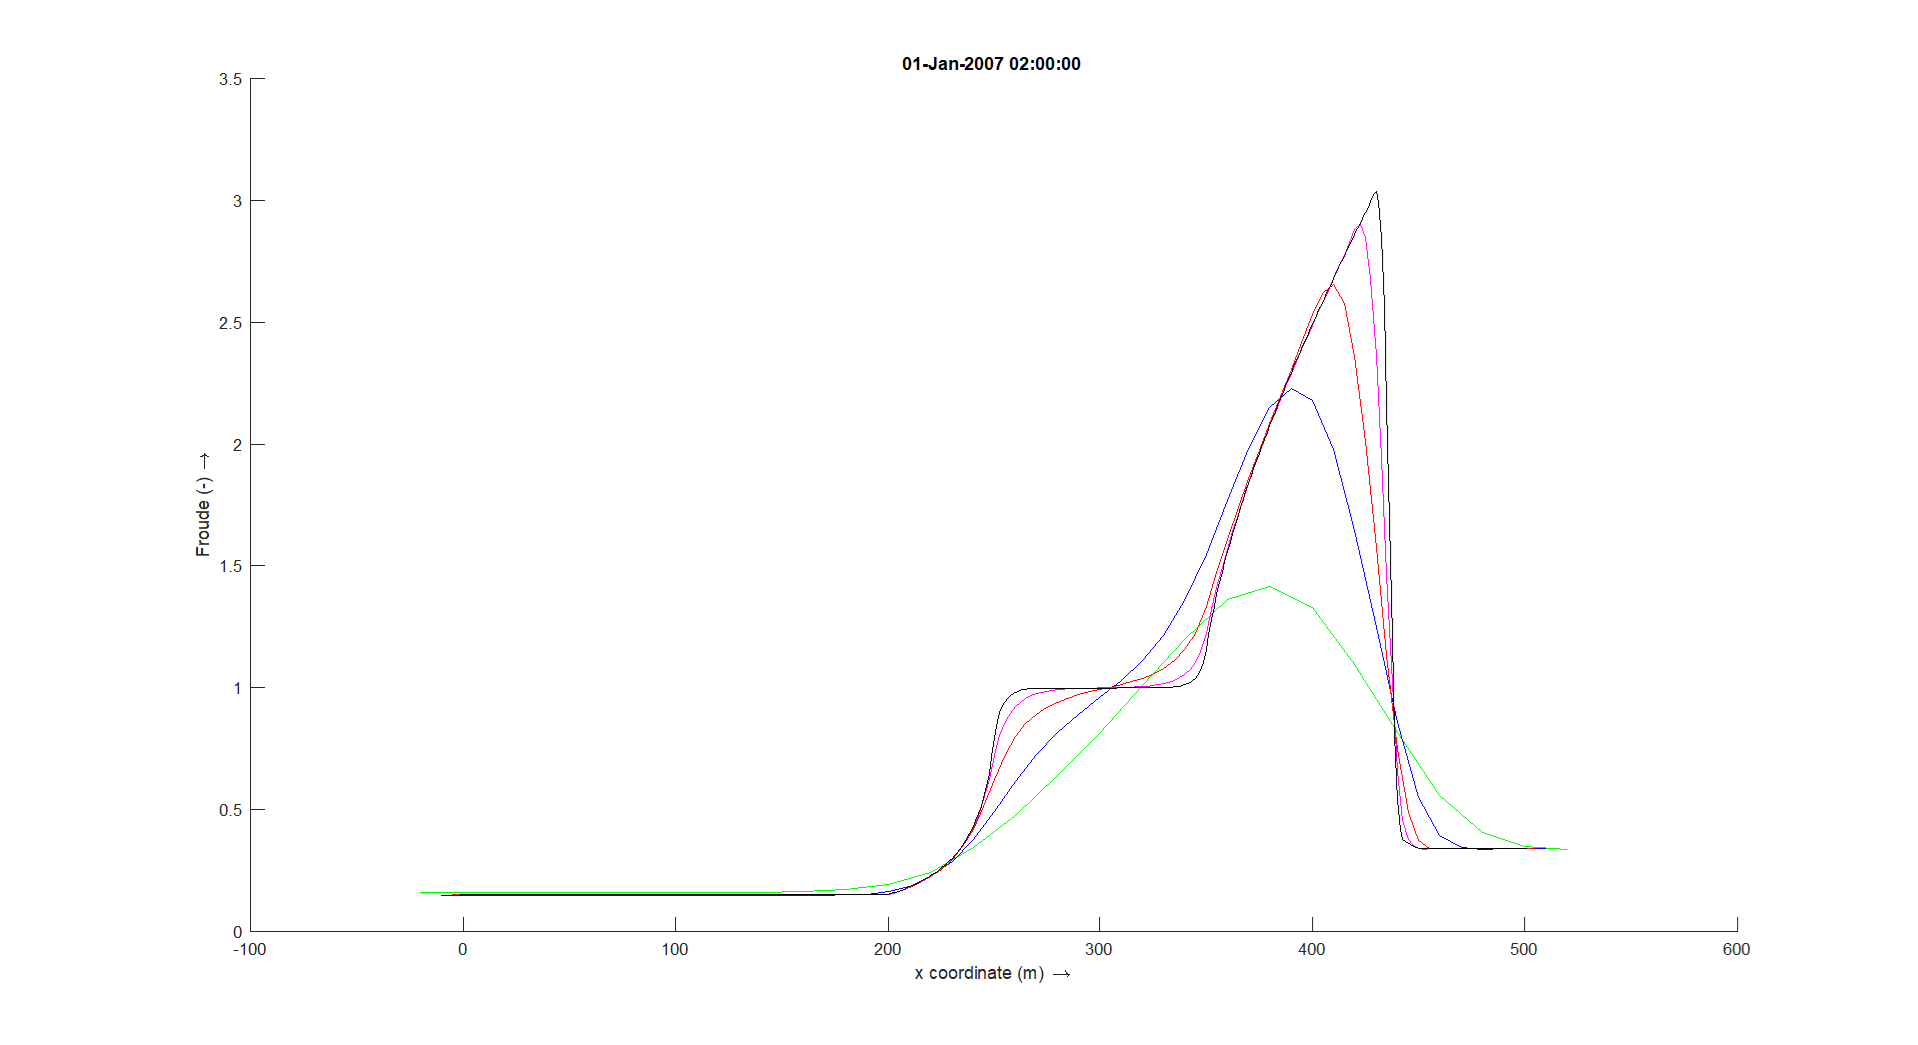
\includegraphics[width=\textwidth]{figures/weir_froude.png}
        \caption{Froude number.}
    \end{subfigure}
    \caption[Weir experiment: Artificial viscosity $\Psi$ and Froude number]{Artificial viscosity $\Psi$ and Froude number. Green: $\Dx = \bqty{20}{\metre}$, $\Dt = \bqty{4}{\second}$;
        Blue: $\Dx = \bqty{10}{\metre}$, $\Dt = \bqty{2}{\second}$;
        Red: $\Dx = \bqty{5}{\metre}$, $\Dt = \bqty{1}{\second}$;
        Cyan: $\Dx = \bqty{2.5}{\metre}$, $\Dt = \bqty{0.5}{\second}$;
        Black: $\Dx = \bqty{1.25}{\metre}$, $\Dt =\bqty{0.25}{\second}$
    }
\end{figure}

%------------------------------------------------------------------------------
%\part{2D Wave}
%-------------------------------------------------------------------------------
\chapter{2-D Shallow water equations}
%-------------------------------------------------------------------------------
Consider the non-linear wave equation
%\begin{subequations}
%    \begin{align}
%        \pdiff{h}{t} + \nabla \dotp \vec{q} & = 0,
%        \\
%        \pdiff{\vec{q}}{t} +  \nabla \dotp \left( \frac{\vec{q}\vec{q}^T}{h} \right) + \half g \nabla h^2 + gh\nabla z_b +   c_f \left( \frac{\vec{q}\abs{\vec{q}}}{h^2} \right) & = 0,
%    \end{align}
%\end{subequations}
%or
\begin{subequations}
    \begin{align}
    \pdiff{h}{t} & + \nabla \dotp \vec{q}  = 0,
    \\
    \pdiff{\vec{q}}{t} & + \nabla \dotp \left( \frac{\vec{q}\vec{q}^T}{h} \right) + gh \nabla \zeta +
    \nonumber \\
    & + c_f \left( \frac{\vec{q}\abs{\vec{q}}}{h^2} \right)
    - \nabla \dotp \left( \nu h \left(  \nabla \vec{q}/h + \nabla \vec{q}^T/h \right) \right) = 0,
    \\
    \zeta & = h + z_b,
\end{align}
\end{subequations}
with
\begin{symbollist}
    \item[$\zeta$] Water level  w.r.t.\ reference plane ($\zeta = h + z_b$), \bunit{\metre}.
    \item[$h$] Water depth ($h = \zeta - z_b$), \bunit{\metre}.
    \item[$z_b$] Bed level  w.r.t.\ reference plane, \bunit{\metre}.
    \item[$\vec{q}$] Flow, defined as $\vec{q} = (q, r)^T = (hu, hv)^T$, \bunit{\square\metre\per\second}.
    \item[$\vec{u}$] Velocity vector, defined as $\vec{u} = (u, v)^T$, \bunit{\metre\per\second}.
    \item[$c_f$] Bed shear stress coefficient, \bunit{-}.
    \begin{itemize}
        \item[Ch\'ezy:] $c_f = g/C^2$
    \end{itemize}
    \item[$C$] Ch\'ezy coefficient, \bunit{\metre^{\half}\, \second^{-1}}.

    \item[$g$] Acceleration due to gravity, \bunit{\metre\per\square\second}.
    \item[$\nu$] Kinematic viscosity, \bunit{\square\metre\per\second}.
\end{symbollist}
\vspace{1cm}
\begin{figure}[H]
    \centering
    \begin{center}
        \def\svgwidth{1.0\textwidth} % scaling text
        \resizebox{0.9\textwidth}{!}{
            \input{figures/definition_variables.pdf_tex}
        }
    \end{center}
    \caption{Definition sketch of water level ($\zeta$), bed level ($z_b$) and total water depth ($h$)}\label{fig:definition_variables_2d}
\end{figure}

\subsection*{Finite Volume approach}
Integrating the equations over a finite volume $\Omega$ yields:
%\begin{subequations}
%    \begin{align}
%        \int_\Omega \pdiff{h}{t}\, d\omega
%        + \int_\Omega \nabla \dotp \vec{q}\, d\omega & = 0,
%        \label{eq:pressure_dependent_on_h_a} \\
%        \int_\Omega \pdiff{\vec{q}}{t}\, d\omega
%        + \int_\Omega \nabla \dotp \left( \frac{\vec{q}\vec{q}^T}{h} \right)\, d\omega
%        + \int_\Omega \half  \nabla \left( g h^2 \right) \, d\omega
%        + \int_\Omega gh\nabla z_b\, d\omega + \int_\Omega c_f \left( \frac{\vec{q}\abs{\vec{q}}}{h^2} \right)\, d\omega & = 0,
%        \label{eq:pressure_dependent_on_h_b}
%    \end{align}
%    \label{eq:pressure_dependent_on_h}
%\end{subequations}
%or
\begin{subequations}
\begin{align}
    \int_\Omega \pdiff{h}{t}\, d\omega &
    + \int_\Omega \nabla \dotp \vec{q}\, d\omega  = 0,
    \label{eq:pressure_dependent_on_zeta_a}
    \\
    \int_\Omega \pdiff{\vec{q}}{t}\, d\omega &
    + \int_\Omega \nabla \dotp \left( \frac{\vec{q}\vec{q}^T}{h} \right)\, d\omega
    + \int_\Omega gh \nabla \zeta\, d\omega +
    \nonumber \\
    & + \int_\Omega c_f \left( \frac{\vec{q}\abs{\vec{q}}}{h^2} \right)\, d\omega
    - \int_\Omega \nabla \dotp \left( \nu h \left(  \nabla \vec{q}/h + \nabla \vec{q}^T/h \right) \right)\, d\omega = 0,
    \label{eq:pressure_dependent_on_zeta_b}
    \\
    \int_\Omega \zeta\, d\omega &
    = \int_\Omega h\, d\omega + \int_\Omega z_b\, d\omega,
    \label{eq:pressure_dependent_on_zeta_c}
\end{align}
\label{eq:pressure_dependent_on_zeta}
\end{subequations}

%-------------------------------------------------------------------------------
\section{Space discretization, structured}
\begin{figure}[H]
    \begin{center}
        \def\svgwidth{0.80\textwidth} % scaling text
        \resizebox{0.65\textwidth}{!}{
            \input{figures/cartesian_grid_interior_2d.pdf_tex}
        }
    \end{center}
    \caption[Definition of the grid to solve the 2D-shallow water equations in the interior area]{Coefficients for the mass-matrix and the control volume in 2-dimensions in the interior area, on a structured grid. The black dots indicate the location of the quadrature points, and black diamonds the flux points.}
    \label{fig:2d_structured_grid}
\end{figure}
For the space discretizations of an arbitrary function $u$ on the quadrature point of a sub-control volume the following space interpolations are used, $u \in \{h,q,r\}$:
\begin{align}
    \left. u\right|_{i+\quart, j+\quart} & \approx \frac{1}{16}\left( 9u_{i, j} + 3 u_{i+1,j} + u_{i+1, j+1} + 3  u_{i, j+1}\right)
    \\
    \left.u\right|_{i+\half, j+\quart} & \approx \frac{1}{8} \left( 3 u_{i,j} + 3 u_{i+1,j} + u_{i+1, j+1} + u_{i, j+1} \right)
    \\
    \left. u \right|_{i+\quart, j+\half} & \approx \frac{1}{8} \left( 3 u_{i, j} + u_{i+1, j+1} + u_{i+1, j}  + 3 u_{i, j+1} \right)
\end{align}
See for the locations \autoref{fig:2d_structured_grid}.
%-------------------------------------------------------------------------------
\subsection{Discretizations continuity equation}
The discretization of continuity \autoref{eq:pressure_dependent_on_zeta_a} will be presented term by term.
%-------------------------------------------------------------------------------
\subsubsection{Time derivative}
The discretization of the time derivative term of the continuity equation reads:
\begin{align}
    \int_{\Omega} \pdiff{h}{t}\, d\omega
\end{align}
which will be approximated by the sum of the integral over the sub-control volumes.
On a structured grid one control volume ($cv$) around a node consist of four sub-control volumes ($scv_i$, $i\in\{1,2,3,4\}$).
\begin{align}
    \int_{cv} \pdiff{h}{t}\, d\omega =
    \int_{scv_1} \pdiff{h}{t}\, d\omega +
    \int_{scv_2} \pdiff{h}{t}\, d\omega +
    \int_{scv_3} \pdiff{h}{t}\, d\omega +
    \int_{scv_4} \pdiff{h}{t}\, d\omega
\end{align}
For a cartesian grid we get:
\begin{align}
    \int_{cv} \pdiff{h}{t}\, d\omega \approx &
    \quart\Dx\Dy\Dtinv \left( h^{n+1,p+1}_{i-\quart, j-\quart} -  h^{n+1,n}_{i-\quart, j-\quart} \right) +
    \nonumber \\*
    &\quart\Dx\Dy\Dtinv \left( h^{n+1,p+1}_{i+\quart, j-\quart} -  h^{n+1,n}_{i+\quart, j-\quart} \right) +
    \nonumber \\*
    &\quart\Dx\Dy\Dtinv \left( h^{n+1,p+1}_{i+\quart, j+\quart} -  h^{n+1,n}_{i+\quart, j+\quart} \right) +
    \nonumber \\*
    &\quart\Dx\Dy\Dtinv \left( h^{n+1,p+1}_{i-\quart, j+\quart} -  h^{n+1,n}_{i-\quart, j+\quart} \right)
\end{align}
Just looking to the quadrature point of $scv_3$ as part of the control volume for node $(i,j)$ the discretization reads:
\begin{align}
    &\quart\Dx\Dy\Dtinv \left( h^{n+1}_{i+\quart, j+\quart} -  h^{n+1,n}_{i+\quart, j+\quart} \right) =
    \\*
    &= \quart\Dx\Dy\Dtinv \left[ \frac{1}{16}\left( 9h^{n+1}_{i, j} + 3 h^{n+1}_{i+1,j}  + 3  h^{n+1}_{i, j+1} + h^{n+1}_{i+1, j+1}\right) \right. +
    \\*
    &\quad - \left. \frac{1}{16}\left( 9 h^{n}_{i, j} +  3 h^{n}_{i+1,j}  + 3  h^{n}_{i, j+1} + h^{n}_{i+1, j+1}\right)\right]
\end{align}
Written in \deltaformulation  it reads:
\begin{align}
    &\quart\Dx\Dy\Dtinv \left( h^{n+1}_{i+\quart, j+\quart} -  h^{n}_{i+\quart, j+\quart} \right) =
    \nonumber \\*
    &=\quart\Dx\Dy\Dtinv \left[ \frac{1}{16}\left( 9 \Delta h^{n+1,p+1}_{i, j} + 3 \Delta q^{n+1,p+1}_{i+1,j+1}  + 3 \Delta q^{n+1,p+1}_{i, j+1} + \Delta h^{n+1,p+1}_{i+1, j+1}\right) \right] +
    \nonumber \\*
    & + \quart\Dx\Dy\Dtinv \left[ \frac{1}{16}\left( 9 h^{n+1,p}_{i, j} + 3 h^{n+1,p}_{i+1,j}  + 3 h^{n+1,p}_{i, j+1} + h^{n+1,p+1}_{i+1, j+1}\right) \right. +
    \nonumber \\*
    &\quad - \left. \frac{1}{16}\left( 9h^{n}_{i, j} +  3 h^{n}_{i+1,j}  + 3  h^{n}_{i, j+1} + h^{n}_{i+1, j+1}\right)\right]
\end{align}

%-------------------------------------------------------------------------------
\subsubsection{Mass flux}
The discretization of the mass flux term of the continuity equation reads:
\begin{align}
\int_\Omega \nabla \dotp \vec{q}\, d\omega =
\oint_{\partial\Omega} \vec{q} \dotp \vec{n} \, dl =
\oint_{\partial\Omega}
\begin{pmatrix}
    q \\
    r
\end{pmatrix}
\dotp
\begin{pmatrix}
    n_x \\
    n_y
\end{pmatrix}
    \, dl
=
\oint_{\partial\Omega} \left( q n_x + r n_y \right) \, dl
\end{align}
with $\vec{n} = (n_x, n_y)^T$ the outward normal vector.

The component for the continuity equation reads:
\begin{align}
    F_{{\it mf}} = q n_x + r n_y
\end{align}

The Jacobian \textbf{at the faces of the control volume} for the mass flux term
reads:
\begin{align}
    %    &\begin{pmatrix}
        %    J_{11} &  J_{12} &  J_{13}
        %    \\
        %     J_{21} &  J_{22} &  J_{23}
        %    \end{pmatrix}
    %    \rightarrow
    &\begin{pmatrix}
        \pdiff{F_{{\it mf}}}{h} & \pdiff{F_{{\it mf}}}{q} & \pdiff{F_{{\it mf}}}{r}
    \end{pmatrix}
    =
    \begin{pmatrix}
        0 & 1 & 1
    \end{pmatrix}
\end{align}
The linearization in time reads:
\begin{align}
    &q^{n+\theta, p} + \theta \Delta q  + r^{n+\theta, p} + \theta \Delta r
\end{align}
This terms need to be computed for each of the control volume faces, taken into account the outward normal.
Eight faces on a structured grid.
For the quadrature point $(i+\half, j+\quart)$ where $\vec{n} = (1,0)^T$ and $1\, dl = \half \Dy$ reads:
\begin{align}
  &\left( q^{n+\theta, p}_{i+\half, j+\quart} + \theta \Delta q_{i+\half, j+\quart}  + r^{n+\theta, p}_{i+\half, j+\quart} + \theta \Delta r_{i+\half, j+\quart} \right) \begin{pmatrix} 1 \\ 0 \end{pmatrix} dl \approx
  \\*
 & \approx \half \Dy\ \frac{1}{8} \left( 3 q^{n+\theta, p}_{i,j} + 3 q^{n+\theta, p}_{i+1,j} + q^{n+\theta, p}_{i+1, j+1} + q^{n+\theta, p}_{i, j+1} \right)
 +
 \\*
 &+ \half \Dy\ \frac{1}{8} \theta \left( 3 \Delta q_{i,j} + 3 \Delta q_{i+1,j} + \Delta q_{i+1, j+1} + \Delta q_{i, j+1} \right)
 \\*
 &+\half \Dy\ \frac{1}{8} \left( 3 r^{n+\theta, p}_{i,j} + 3 r^{n+\theta, p}_{i+1,j} + r^{n+\theta, p}_{i+1, j+1} + r^{n+\theta, p}_{i, j+1} \right)
\\*
&+ \half \Dy\ \frac{1}{8} \theta \left( 3 \Delta r_{i,j} + 3 \Delta r_{i+1,j} + \Delta r_{i+1, j+1} + \Delta r_{i, j+1} \right)
\\*
\end{align}
%-------------------------------------------------------------------------------
\subsection{Discretizations momentum equations}
The discretization of momentum \autoref{eq:pressure_dependent_on_zeta_b} will be presented term by term.
%--------------------------------------------------------------------------------
\subsubsection{Time derivative}
The discretization of the time derivative term of the momentum equation is only shown for the q-momentum equation, the time derivative for the r-momentum equation is similar. The time derivation for hte q-momentum equation reads:
\begin{align}
    \int_{\Omega} \pdiff{q}{t}\, d\omega
\end{align}
which will be approximated by the sum of the integral over the sub-control volumes.
On a structured grid one control volume ($cv$) around a node consist of four sub-control volumes ($scv_i$, $i\in\{1,2,3,4\}$).
\begin{align}
    \int_{cv} \pdiff{q}{t}\, d\omega =
    \int_{scv_1} \pdiff{q}{t}\, d\omega +
    \int_{scv_2} \pdiff{q}{t}\, d\omega +
    \int_{scv_3} \pdiff{q}{t}\, d\omega +
    \int_{scv_4} \pdiff{q}{t}\, d\omega
\end{align}
For a cartesian grid we get:
\begin{align}
    \int_{cv} \pdiff{q}{t}\, d\omega \approx &
    \quart\Dx\Dy\Dtinv \left( q^{n+1}_{i-\quart, j-\quart} -  q^{n}_{i-\quart, j-\quart} \right) +
    \nonumber \\*
    &\quart\Dx\Dy\Dtinv \left( q^{n+1}_{i+\quart, j-\quart} -  q^{n}_{i+\quart, j-\quart} \right) +
    \nonumber \\*
    &\quart\Dx\Dy\Dtinv \left( q^{n+1}_{i+\quart, j+\quart} -  q^{n}_{i+\quart, j+\quart} \right) +
    \nonumber \\*
    &\quart\Dx\Dy\Dtinv \left( q^{n+1}_{i-\quart, j+\quart} -  q^{n}_{i-\quart, j+\quart} \right)
\end{align}
Just looking to the quadrature point of $scv_3$ as part of the control volume for node $(i,j)$ the discretization reads:
\begin{align}
    &\quart\Dx\Dy\Dtinv \left( q^{n+1}_{i+\quart, j+\quart} -  q^{n}_{i+\quart, j+\quart} \right) =
    \nonumber \\*
    &= \quart\Dx\Dy\Dtinv \left[ \frac{1}{16}\left( 9 q^{n+1}_{i, j} + 3 q^{n+1}_{i+1,j}  + 3 q^{n+1}_{i, j+1} + q^{n+1}_{i+1, j+1}\right) \right. +
    \nonumber\\*
    &\quad - \left. \frac{1}{16}\left( 9 q^{n}_{i, j} +  3 q^{n}_{i+1,j}  + 3  q^{n}_{i, j+1} + q^{n}_{i+1, j+1}\right)\right]
\end{align}
Written in \deltaformulation  it reads:
\begin{align}
    &\quart\Dx\Dy\Dtinv \left( q^{n+1}_{i+\quart, j+\quart} -  q^{n}_{i+\quart, j+\quart} \right) =
    \nonumber \\*
    &=\quart\Dx\Dy\Dtinv \left[ \frac{1}{16}\left( 9 \Delta q^{n+1,p+1}_{i, j} + 3 \Delta q^{n+1,p+1}_{i+1,j+1}  + 3 \Delta q^{n+1,p+1}_{i, j+1} + \Delta q^{n+1,p+1}_{i+1, j+1}\right) \right] +
    \nonumber \\*
    & + \quart\Dx\Dy\Dtinv \left[ \frac{1}{16}\left( 9 q^{n+1,p}_{i, j} + 3 q^{n+1,p}_{i+1,j}  + 3 q^{n+1,p}_{i, j+1} + q^{n+1,p+1}_{i+1, j+1}\right) \right. +
    \nonumber \\*
    &\quad - \left. \frac{1}{16}\left( 9 q^{n}_{i, j} +  3 q^{n}_{i+1,j}  + 3  q^{n}_{i, j+1} + q^{n}_{i+1, j+1}\right)\right]
\end{align}
%--------------------------------------------------------------------------------
\subsubsection{Pressure term} \label{sec:linearized_pressure_zeta}
In this section we use that the pressure term is dependent on $\zeta$.
\begin{align}
    \int_{\Omega} gh \nabla \zeta \, d\omega
\end{align}
The integral over a control volume will be a sum of integrals over the sub control volumes.
On a structured grid one control volume ($cv$) around a node consist of four sub-control volumes ($scv_i$, $i\in\{1,2,3,4\}$).
\begin{align}
    \int_{cv}    gh \nabla \zeta\, d\omega =
    \int_{scv_1} gh \nabla \zeta\, d\omega +
    \int_{scv_2} gh \nabla \zeta\, d\omega +
    \int_{scv_3} gh \nabla \zeta\, d\omega +
    \int_{scv_4} gh \nabla \zeta\, d\omega
\end{align}


Considering one sub-control volume and only for the $x$-direction (assuming a cartesian grid) then it reads:
\begin{align}
    & \int_{\textit{scv}} gh \nabla \zeta \, d\omega  \approx
    \\
    & \approx \quart \Dx\Dy\, g h^{n+\theta,p+1}_{qp} \pdiff{\zeta^{n+\theta,p+1}_{qp}}{x}
    \approx \\
   & \approx \quart  \Dx\Dy\, g \left( h^{n+\theta,p}_{qp} + \theta \Delta h^{n+1,p+1}\right)  \pdiff{}{x}\left(\zeta^{n+\theta,p}_{qp} + \theta \Delta \zeta^{n+1,p+1}_{qp}\right)
\end{align}
with $qp$ the location of the quadrature point in the sub-control volume.
Assume that the higher order terms are negligible then the discretization for each of the 4 sub-control volumes reads:
\begin{align}
        \quart  \Dx\Dy\, g \left(
        h^{n+\theta, p}_{qp} \pdiff{\zeta^{n+\theta, p}_{qp}}{x}
        + h^{n+\theta, p}_{qp} \pdiff{}{x} (\theta \Delta \zeta^{n+1, p+1}_{qp})
        + \pdiff{\zeta^{n+\theta, p}_{qp}}{x} \theta \Delta h^{n+1,p+1}_{qp}
          \right)
\end{align}
Just looking to the quadrature point of $scv_3$ as part of the control volume for node $(i,j)$ the discretization reads:
\begin{align}
    \quart  \Dx\Dy\, g \left(
    h^{n+\theta, p}_{i+\quart, j+\quart} \pdiff{\zeta^{n+\theta, p}_{i+\quart, j+\quart}}{x}
    + h^{n+\theta, p}_{i+\quart, j+\quart} \pdiff{}{x}(\theta \Delta \zeta^{n+1, p+1}_{i+\quart, j+\quart})
    + \pdiff{\zeta^{n+\theta, p}_{i+\quart, j+\quart}}{x} \theta \Delta h^{n+1,p+1}_{i+\quart, j+\quart}
    \right)
\end{align}
with
\begin{align}
    h^{n+\theta, p}_{i+\quart, j+\quart} & \approx
    \frac{1}{16}\left( 9h^{n+\theta, p}_{i, j} + 3 h^{n+\theta, p}_{i+1,j} + h^{n+\theta, p}_{i+1, j+1} + 3  h^{n+\theta, p}_{i, j+1}\right)
    \\*
    \pdiff{\zeta^{n+\theta, p}_{i+\quart, j+\quart}}{x} & \approx
   \frac{1}{\Dx}\quart\left[ 3 \left(\zeta_{i,j} - \zeta_{i+1,j}\right) + \left( \zeta_{i,j+1} - \zeta_{i+1,j+1}\right) \right]
   \\*
   \pdiff{\Delta \zeta^{n+1, p+1}_{i+\quart, j+\quart}}{x} & \approx
   \frac{1}{\Dx}\quart\left[ 3 \left(\Delta\zeta^{n+1, p+1}_{i,j} - \Delta\zeta^{n+1, p+1}_{i+1,j}\right) + \left(\Delta\zeta^{n+1, p+1}_{i,j+1} - \Delta\zeta^{n+1, p+1}_{i+1,j+1} \right) \right]
   \\*
   \Delta h^{n+1,p+1}_{i+\quart, j+\quart} & \approx
   \frac{1}{16}\left( 9\Delta h^{n+1,p+1}_{i, j} + 3 \Delta h^{n+1,p+1}_{i+1,j} + \Delta h^{n+1,p+1}_{i+1, j+1} + 3  \Delta h^{n+1,p+1}_{i, j+1}\right)
\end{align}
\paragraph*{Example}
Set $\Delta x = \bqty{100}{\metre}$, $\lpdiff{\zeta}{x}=0$, estimate the coefficients in the matrix for a single sub-control volume:
\begin{align}
    \Delta h_{i,j} = \quart \Dx\Dy g \frac{1}{16} \left[ 9\ 3\ 1\ 3  \right] = \num{1562.5} \times  \left[ 9\ 3\ 1\ 3  \right]
\end{align}
%--------------------------------------------------------------------------------
\subsubsection{Convection}
The convection term in vector notation reads:
\begin{align}
    \int_\Omega \nabla \dotp \left( \frac{\vec{q}\vec{q}^T}{h} \right)\, d\omega =
    \oint_{\Omega}  \left( \frac{\vec{q}\vec{q}^T}{h} \right) \dotp \vec{n} \, dl =
    \oint_{\Omega}
    \begin{pmatrix}
        qq/h & qr/h \\
        rq/h & rr/h
    \end{pmatrix}
    \dotp
    \begin{pmatrix}
        n_x \\
        n_y
    \end{pmatrix}
     \, dl
\end{align}
with $\vec{n} = (n_x, n_y)^T$ the outward normal vector.

The components for the two momentum equations read:
\begin{align}
    F_q
    & = \oint_{\Omega} \left(\frac{qq}{h}{n_x} + \frac{qr}{h}{n_y}\right) \, dl
    \qquad \textit{q-momentum eq.}
    \\
    F_r
    & = \oint_{\Omega} \left(\frac{rq}{h}{n_x} + \frac{rr}{h}{n_y}\right) \, dl
    \qquad \textit{r-momentum eq.}
\end{align}
%The Jacobian \textbf{at the faces of the control volume} for each term of the convection term reads:
%\begin{align}
%    &\begin{pmatrix}
%        \pdiff{}{h}(\frac{qq}{h}) & \pdiff{}{q}(\frac{qq}{h}) & \pdiff{}{r}(\frac{qq}{h})
%    \end{pmatrix}
%    =
%    \begin{pmatrix}
%    - \frac{qq}{h^2} & \frac{2q}{h}  & 0
%    \end{pmatrix}
%\\
%    &\begin{pmatrix}
%    \pdiff{}{h}(\frac{qr}{h}) & \pdiff{}{q}(\frac{qr}{h}) & \pdiff{}{r}(\frac{qr}{h})
%\end{pmatrix}
%=
%\begin{pmatrix}
%    - \frac{qr}{h^2} & \frac{r}{h}  & \frac{q}{h}
%\end{pmatrix}
%\\
%    &\begin{pmatrix}
%    \pdiff{}{h}(\frac{rq}{h}) & \pdiff{}{q}(\frac{rq}{h}) & \pdiff{}{r}(\frac{rq}{h})
%\end{pmatrix}
%=
%\begin{pmatrix}
%    - \frac{rq}{h^2} & \frac{r}{h}  & \frac{q}{h}
%\end{pmatrix}
%\\
%    &\begin{pmatrix}
%    \pdiff{}{h}(\frac{rr}{h}) & \pdiff{}{q}(\frac{rr}{h}) & \pdiff{}{r}(\frac{rr}{h})
%\end{pmatrix}
%=
%\begin{pmatrix}
%    - \frac{rr}{h^2} & 0 & \frac{2r}{h}
%\end{pmatrix}
%\end{align}
%
The linearization in time for the $q$-momentum equation reads (see \autoref{eq:2d_convection_q_equation}):
\begin{align}
    &\frac{q^{n+\theta, p}_{qp}q^{n+\theta, p}_{qp}}{h^{n+\theta, p}_{qp}} n_x+ \frac{q^{n+\theta, p}_{qp}r^{n+\theta, p}_{qp}}{h^{n+\theta, p}_{qp}} n_y
    + \left( -\frac{q^{n+\theta, p}_{qp}q^{n+\theta, p}_{qp}}{(h^{n+\theta, p}_{qp})^2} n_x -
    \frac{q^{n+\theta, p}_{qp}r^{n+\theta, p}_{qp}}{(h^{n+\theta, p}_{qp})^2} n_y \right) \theta \Delta h +
    \nonumber \\*
    & + \left( \frac{2 q^{n+\theta, p}_{qp}}{h^{n+\theta, p}_{qp}} n_x +  \frac{r^{n+\theta, p}_{qp}}{h^{n+\theta, p}_{qp}} n_y \right) \theta \Delta q
    + \left( 0\, n_x + \frac{q^{n+\theta, p}_{qp}}{h^{n+\theta, p}_{qp}} n_y \right) \theta \Delta r
\end{align}
and for the $r$-momentum equation:
\begin{align}
    &\frac{r^{n+\theta, p}_{qp}q^{n+\theta, p}_{qp}}{h^{n+\theta, p}_{qp}} n_x+
     \frac{r^{n+\theta, p}_{qp}r^{n+\theta, p}_{qp}}{h^{n+\theta, p}_{qp}} n_y
   + \left( -\frac{r^{n+\theta, p}_{qp}q^{n+\theta, p}_{qp}}{(h^{n+\theta, p}_{qp})^2} n_x -
\frac{r^{n+\theta, p}_{qp}r^{n+\theta, p}_{qp}}{(h^{n+\theta, p}_{qp})^2} n_y \right) \theta \Delta h +
\nonumber \\*
& +
\left( \frac{r^{n+\theta, p}_{qp}}{h^{n+\theta, p}_{qp}} n_x  + 0\, n_y \right) \theta \Delta q +
\left (
\frac{q^{n+\theta, p}_{qp}}{h^{n+\theta, p}_{qp}} n_x
+ \frac{2 r^{n+\theta, p}_{qp}}{h^{n+\theta, p}_{qp}} n_y \right) \theta \Delta r
\end{align}

This terms need to be computed for each of the control volume faces, taken into account the outward normal.
Eight faces on a cartesian/curvilinear grid.

%--------------------------------------------------------------------------------
\subsubsection{Bed shear stress}
The bed shear stress  term in vector notation reads:
\begin{align}
    \int_\Omega c_f \left( \frac{\vec{q}\abs{\vec{q}}}{h^2} \right)\, d\omega.
\end{align}
The components for the two momentum equations read:
\begin{align}
    F_q = \int_\Omega c_f \left( \frac{q\abs{\vec{q}}}{h^2} \right)\, d\omega, \qquad \textit{q-momentum eq.}
    \\
    F_r = \int_\Omega c_f \left( \frac{r\abs{\vec{q}}}{h^2} \right)\, d\omega, \qquad \textit{r-momentum eq.}
\end{align}
and $\abs{\vec{q}} = \sqrt{q^2 + r^2}$.
To avoid the discontinuity in the first derivative around zero, the absolute function will be approximated by (the Newton iteration process needs $C^1$--continue functions)
\begin{align}
    \abs{\vec{q}} \approx \abs{\widetilde{\vec{q}}} = \left( (q^2 + r^2)^2 + \eps^4 \right)^\quart.
\end{align}
The bed shear stress then reads:
\begin{align}
    F_q \approx \Dx\Dy\, c_f \left( \frac{q\abs{\widetilde{\vec{q}}}}{h^2} \right), \qquad \textit{q-momentum eq.}
    \\
    F_r \approx \Dx\Dy\, c_f \left( \frac{r\abs{\widetilde{\vec{q}}}}{h^2} \right), \qquad \textit{r-momentum eq.}
\end{align}
The Jacobian for the bed shear stress $F(h,q,r)$ reads:
\begin{align}
%    &\begin{pmatrix}
%    J_{11} &  J_{12} &  J_{13}
%    \\
%     J_{21} &  J_{22} &  J_{23}
%    \end{pmatrix}
%    \rightarrow
    &\begin{pmatrix}
        \pdiff{F_q}{h} & \pdiff{F_q}{q} & \pdiff{F_q}{r}
        \\
        \pdiff{F_r}{h} & \pdiff{F_r}{q} & \pdiff{F_r}{r}
    \end{pmatrix}
    =
    \\
    &=
    \begin{pmatrix}
       -2c_f \frac{q\abs{\widetilde{\vec{q}}}}{h^3}
       & c_f\frac{\abs{\widetilde{\vec{q}}}}{h^2}
       + c_f \frac{q}{h^2} \frac{q(q^2+ r^2)}{\abs{\widetilde{\vec{q}}}^3}
       & c_f \frac{q}{h^2}\frac{r(q^2+ r^2)}{\abs{\widetilde{\vec{q}}}^3}
       \\
       -2c_f \frac{r\abs{\widetilde{\vec{q}}}}{h^3}
       & c_f \frac{r}{h^2}\frac{q(q^2+ r^2)}{\abs{\widetilde{\vec{q}}}^3}
       & c_f\frac{\abs{\widetilde{\vec{q}}}}{h^2}
       + c_f \frac{r}{h^2}\frac{r(q^2+ r^2)}{\abs{\widetilde{\vec{q}}}^3}
    \end{pmatrix}
\end{align}
All these coefficients of the Jacobian should be evaluated at the quadrature point of the sub-control volumes and evaluated at time level $(n+\theta,p)$.
The same applies also for the right hand side and evaluated at time level $(n+\theta,p)$.

The linearization in time for the $q$-momentum equation reads (see \autoref{eq:2d_convection_q_equation}):
\begin{align}
        &c_f \left( \frac{q^{n+\theta,p}_{qp}\abs{\widetilde{\vec{q}^{n+\theta,p}}}}{(h^{n+\theta,p}_{qp})^2} \right)
        - \left( 2 c_f \frac{ q^{n+\theta,p}_{qp} \abs{\widetilde{\vec{q}^{n+\theta,p}_{qp}}} }{(h^{n+\theta,p}_{qp})^3} \right) \theta \Delta h_{qp} +
        \\*
        & \quad +
        \left( c_f \frac{\abs{\widetilde{\vec{q}^{n+\theta,p}_{qp}}}}{(h^{n+\theta,p}_{qp})^2}
        + c_f \frac{q^{n+\theta,p}_{qp}}{(h^{n+\theta,p}_{qp})^2} \frac{q^{n+\theta,p}_{qp}\left( (q^{n+\theta,p}_{qp})^2 + (r^{n+\theta,p}_{qp})^2 \right) }{\abs{\widetilde{\vec{q}^{n+\theta,p}_{qp}}}^3} \right) \theta \Delta q_{qp} +
        \\*
        & \quad + \left( c_f \frac{q^{n+\theta,p}_{qp}}{(h^{n+\theta,p}_{qp})^2}
        \frac{ r^{n+\theta,p}_{qp} \left( (q^{n+\theta,p}_{qp})^2 + (r^{n+\theta,p}_{qp})^2  \right)}
        {\abs{\widetilde{\vec{q}^{n+\theta,p}_{qp}}}^3 } \right) \theta \Delta r_{qp}
 \end{align}
and for the $r$-momentum equation:
\begin{align}
        &c_f \left( \frac{r^{n+\theta,p}_{qp}\abs{\widetilde{\vec{q}^{n+\theta,p}}}}{(h^{n+\theta,p}_{qp})^2} \right)
        - \left( 2 c_f \frac{ r^{n+\theta,p}_{qp} \abs{\widetilde{\vec{q}^{n+\theta,p}_{qp}}}} {(h^{n+\theta,p}_{qp})^3} \right) \theta \Delta h_{qp} +
        \\*
        & \quad + \left(
         c_f \frac{r^{n+\theta,p}_{qp}}{(h^{n+\theta,p}_{qp})^2}\frac{q^{n+\theta,p}_{qp}\left( (q^{n+\theta,p}_{qp})^2 + (r^{n+\theta,p}_{qp})^2 \right)}
        {\abs{\widetilde{\vec{q}^{n+\theta,p}_{qp}}}^3 }
        \right) \theta \Delta q_{qp} +
        \\*
        &\quad + \left( c_f \frac{\abs{\widetilde{\vec{q}^{n+\theta,p}_{qp}}}}{(h^{n+\theta,p}_{qp})^2}
        + c_f \frac{r^{n+\theta,p}_{qp}}{(h^{n+\theta,p}_{qp})^2} \frac{r^{n+\theta,p}_{qp}\left( (q^{n+\theta,p}_{qp})^2 + (r^{n+\theta,p}_{qp})^2 \right) }{\abs{\widetilde{\vec{q}^{n+\theta,p}_{qp}}}^3}  \right) \theta \Delta r_{qp}
\end{align}
with
\begin{align}
    \abs{\widetilde{\vec{q}^{n+\theta,p}_{qp}}} = \left( (q^2_{qp} + r^2_{qp})^2 + \eps^4 \right)^\quart.
\end{align}
These terms need to be computed for each quadrature points ($qp$) of the sub-control volumes.
%--------------------------------------------------------------------------------
\subsubsection{Viscosity}
The viscosity term in vector notation reads:
\begin{align}
    \int_\Omega \nabla \dotp \left( \nu h \left(  \nabla (\vec{q}/h) + \nabla (\vec{q}^T/h) \right) \right)\, d\omega =
    \oint_{\Omega}  \left( \nu h \left( \nabla (\vec{q}/h) + \nabla (\vec{q}^T/h) \right) \right) \dotp \vec{n}\, dl
\end{align}
with $\vec{n} = (n_x, n_y)^T$ the outward normal vector.
Written in components ($\vec{q} = (q, r)^T$):
\begin{align}
    &\oint_{\Omega}  \left( \nu h \left( \nabla (\vec{q}/h) + \nabla (\vec{q}^T/h) \right) \right) \dotp \vec{n}\, dl =
    \\
    & =
    \oint_{\Omega} \nu h
    \left(
    \begin{pmatrix}
    \pdiff{(q/h)}{x} & \pdiff{(q/h)}{y}
    \\
    \pdiff{(r/h)}{x} & \pdiff{(r/h)}{y}
    \end{pmatrix}
    +
    \begin{pmatrix}
    \pdiff{(q/h)}{x} & \pdiff{(r/h)}{x}
    \\
    \pdiff{(q/h)}{y} & \pdiff{(r/h)}{y}
   \end{pmatrix}
   \right)
    \dotp \vec{n}\, dl
\end{align}
The components for the two momentum equations read:
\begin{align}
    F_q
    & = \oint_{\Omega} \nu h
    \left[ 2\pdiff{(q/h)}{x} n_x
    + \left(\pdiff{(q/h)}{y} + \pdiff{(r/h)}{x}\right)n_y \right] \, dl
    \qquad \textit{q-momentum eq.}
    \\
    F_r
    & = \oint_{\Omega}  \nu h
    \left[ \left(\pdiff{(r/h)}{x} + \pdiff{(q/h)}{y}\right)n_x
    + 2\pdiff{(r/h)}{y} n_y \right] \, dl
    \qquad \textit{r-momentum eq.}
\end{align}
where
\begin{align}
    \cal{A}: & \quad \nu h \pdiff{(q/h)}{x} = \nu \left( \pdiff{q}{x} - \frac{q}{h}\pdiff{h}{x} \right)
    \\
    \cal{B}: & \quad \nu h \pdiff{(q/h)}{y} = \nu \left( \pdiff{q}{y} - \frac{q}{h}\pdiff{h}{y} \right)
    \\
    \cal{C}: & \quad \nu h \pdiff{(r/h)}{x} = \nu \left( \pdiff{r}{x} - \frac{r}{h}\pdiff{h}{x} \right)
    \\
    \cal{D}: & \quad \nu h \pdiff{(r/h)}{y} = \nu \left( \pdiff{r}{y} - \frac{r}{h}\pdiff{h}{y} \right)
\end{align}
These equations need to be  discretized on the quadrature points $qp$ at the control volume faces.
The discretization is first  given for expression $\cal{A}$ (using result from \autoref{sec:jacobians_with_non_linear_quotient_term} for the quotient):
\begin{align}
     & \nu_{qp} \pdiff{q^{n+\theta, p+1}_{qp}}{x}  -
    \nu_{qp} \frac{q^{n+\theta, p+1}}{h^{n+\theta, p+1}_{qp}}\pdiff{ h^{n+\theta, p+1}_{qp}}{x} \approx
    \\
    & \approx
%    \nu_{qp} \pdiff{(q^{n+\theta,p}_{qp} +  \theta \Delta q_{qp})}{x}
%    - \nu_{qp} \frac{(q^{n+\theta,p}_{qp} +  \theta \Delta q_{qp})}{h^{n+\theta,p}_{qp}} (1 -  \frac{1}{h^{n+\theta,p}_{qp}}\theta \Delta h_{qp})  \pdiff{(h^{n+\theta,p}_{qp} +  \theta \Delta h_{qp})}{x} =
%    \\
%    & =
    \nu_{qp} \pdiff{q^{n+\theta,p}_{qp}}{x} + \nu_{qp} \pdiff{}{x}(\theta \Delta q_{qp}) +
    \nonumber \\
    &- \nu_{qp} \left(
    \frac{q^{n+\theta,p}_{qp}}{h^{n+\theta,p}_{qp}} - \frac{q^{n+\theta,p}_{qp}}{(h^{n+\theta,p}_{qp})^2} \theta \Delta h_{qp} +
    \frac{1}{h^{n+\theta,p}_{qp}} \theta \Delta q_{qp}
    \right)\left(  \pdiff{h^{n+\theta,p}_{qp}}{x} +   \pdiff{}{x}(\theta \Delta h_{qp}) \right) \approx
    \\
    & \approx
    \nu_{qp} \left( \pdiff{q^{n+\theta,p}_{qp}}{x} - \frac{q^{n+\theta,p}_{qp}}{h^{n+\theta,p}_{qp}} \pdiff{h^{n+\theta,p}_{qp}}{x} \right)
    %
    \\
& + \nu_{qp}  \frac{q^{n+\theta,p}_{qp}}{(h^{n+\theta,p}_{qp})^2} \pdiff{h^{n+\theta,p}_{qp}}{x}  \theta \Delta h_{qp}
- \nu_{qp} \frac{1}{h^{n+\theta,p}_{qp}}  \pdiff{h^{n+\theta,p}_{qp}}{x} \theta \Delta q_{qp}
    \\
    & +
    \nu_{qp} \pdiff{}{x}(\theta \Delta q_{qp}) +
    \nu_{qp} \frac{q^{n+\theta,p}_{qp}}{h^{n+\theta,p}_{qp}} \pdiff{}{x}(\theta \Delta h_{qp})
\end{align}
the terms $O(\Delta h\pdiff{\Delta h}{x}, \Delta q \pdiff{\Delta h}{x})$ are assumed to negligible.
In a similar way for the other three expressions:
\begin{align}
    \cal{B}: & \quad \nu_{qp} \pdiff{q^{n+\theta, p+1}_{qp}}{y}  -
\nu_{qp} \frac{q^{n+\theta, p+1}}{h^{n+\theta, p+1}_{qp}}\pdiff{ h^{n+\theta, p+1}_{qp}}{y}
\\
    \cal{C}: & \quad \nu_{qp} \pdiff{r^{n+\theta, p+1}_{qp}}{x}  -
\nu_{qp} \frac{r^{n+\theta, p+1}}{h^{n+\theta, p+1}_{qp}}\pdiff{ h^{n+\theta, p+1}_{qp}}{x}
\\
    \cal{D}: & \quad \nu_{qp} \pdiff{r^{n+\theta, p+1}_{qp}}{x}  -
\nu_{qp} \frac{r^{n+\theta, p+1}}{h^{n+\theta, p+1}_{qp}}\pdiff{ h^{n+\theta, p+1}_{qp}}{x}
\end{align}



This terms need to be computed for each of the control volume faces, taken into account the outward normal.
Eight faces on a cartesian/curvilinear grid.


%%--------------------------------------------------------------------------------
%\subsubsection{Pressure term, dependent on $h$}
%In this section we use that the pressure term is dependent on $h$.
%\begin{align}
%    \int_{\Omega_i} \half  \nabla \left( g h^2\right) \, d\omega & =
%    \int_{\partial\Omega_i} \half  g h^2 \vec{\hat n}\, dl \label{eq:2d_press_term}
%\end{align}
%The linearization of the pressure term in the momentum equation around iteration level $p$ read:
%\begin{align}
%    \half g \left(h^{n+\theta,p+1}_{\partial\Omega_i}\right)^2  & =
%    \half g \left(h^{n+\theta,p+1}_{\partial\Omega_i}\right)^2
%    + g h^{n+\theta,p+1}_{\partial\Omega_i} \left({h}^{n+\theta,p+1} - {h}^{n+\theta,p}\right) =
%    \\
%    & = \half g \left(h^{n+\theta,p+1}_{\partial\Omega_i}\right)^2 + \theta  g h^{n+\theta,p+1}_{\partial\Omega_j} \Delta {h}^{n+1,p+1}
%\end{align}
%
%The component in $x$-direction read:
%\begin{align}
%    \int_{\partial\Omega_i} & \half  g h^2 \vec{\hat n} \dotp \vec{i_x}\, dl \approx
%    \nonumber \\
%    \approx  & \Dy \left( \half g \left(h^{n+\theta,p}_{i+\half,j}\right)^2 + \theta  g h^{n+\theta,p+1}_{i+\half,j} \Delta {h}^{n+1,p+1}_{i+\half,j}  \right) +
%    \nonumber \\
%    - & \Dy \left( \half g \left(h^{n+\theta,p}_{i-\half,j}\right)^2 + \theta  g h^{n+\theta,p+1}_{i-\half,j} \Delta {h}^{n+1,p+1}_{i-\half,j}  \right)
%\end{align}
%The component in $y$-direction read:
%\begin{align}
%    \int_{\partial\Omega_i} & \half  g h^2 \vec{\hat n} \dotp \vec{i_y}\, dl \approx
%    \nonumber \\
%    \approx  & \Dx \left( \half g \left(h^{n+\theta,p}_{i,j+\half}\right)^2 + \theta  g h^{n+\theta,p+1}_{i,j+\half} \Delta {h}^{n+1,p+1}_{i,j+\half}  \right) +
%    \nonumber \\
%    - & \Dx \left( \half g \left(h^{n+\theta,p}_{i,j-\half}\right)^2 + \theta  g h^{n+\theta,p+1}_{i,j-\half} \Delta {h}^{n+1,p+1}_{i,j-\half}  \right)
%\end{align}
%%-------------------------------------------------------------------------------
%\section{Space discretization, unstructured}
%\notyet
%------------------------------------------------------------------------------
\subsection{Discretization at boundary}
\begin{figure}[H]
    \begin{center}
        \def\svgwidth{0.80\textwidth} % scaling text
        \resizebox{0.65\textwidth}{!}{
            \input{figures/cartesian_grid_along_straight_boundary_essential_natural.pdf_tex}
        }
    \end{center}
    \caption[Definition of the grid to solve the 2D-shallow water equations at the boundary]{Coefficients of the mass-matrix in 2-dimensions on a structured grid along a straight boundary. The essential boundary condition is located at the cyan-colored line and the natural boundary condition at the orange line.}
    \label{fig:structured_grid_along_straight_boundary}
\end{figure}
For the 2D non-linear wave equations (\autoref{eq:pressure_dependent_on_zeta}) at each boundary boundary conditions need to be prescribed, the number of boundary conditions depends on the flow direction on the boundary.
Considering a hyperbolic system, if the flow is flowing into the domain two boundary conditions need to prescribed and when the flow is flowing out the domain just one boundary need to prescribed.
This is according the characteristic theory of 2D hyperbolic systems \citep{DaubertEtGraffe1967}.
The ingoing information is called the \textbf{essential} boundary condition (Dirichlet or Neumann condition).
And a boundary condition to handle the outgoing wave is called the \textbf{natural} boundary condition.
So for inflow there are \textbf{two essential} and \textbf{one natural} boundary condition and for outflow there is \textbf{one} \textbf{essential} boundary condition and \textbf{two} \textbf{natural} boundary conditions.

The boundary conditions in this section are presented for the left/west boundary.
First the \textbf{essential} boundary conditions are discussed and after that the \textbf{natural} boundary condition.
A similar derivation can be given for right/east boundary.

%------------------------------------------------------------------------------
\subsubsection{Essential boundary condition}
The \textbf{essential} boundary condition is to be assumed somewhere in the first control volume, ($x_{i_{bc}}$ with $i_{bc} \in [i-\half, i+\half]$ ).
For simplicity the boundary condition is chosen to be on node $i=1$ (location $x_{1}$).

\begin{figure}[H]
    \begin{center}
        \def\svgwidth{0.80\textwidth} % scaling text
        \resizebox{0.65\textwidth}{!}{
            \input{figures/cartesian_grid_along_straight_boundary_essential.pdf_tex}
        }
    \end{center}
    \caption{Essential boundary condition, dotted lines indicate the border of the control volumes.}    \label{fig:structured_grid_along_straight_boundary_essential}
\end{figure}
The \textbf{essential} boundary condition for the left/west boundary at $x_{1}$ reads, describing the ingoing wave (indicated with $h^+$, $q^+$, $r^+$) with as less as possible disturbing the outgoing wave (\autoref{eq:left_right_going_equations}):
\begin{align}
    \left(\sqrt{gh} - \frac{q}{h}\right) \pdiff{h^{+}}{t} + \pdiff{q^{+}}{t} & = F(t)
    \label{eq:essential_conv_2d_1}
    \\
    \left(\sqrt{gh} + \frac{q}{h}\right) \pdiff{h^{+}}{t} - \pdiff{q^{+}}{t} & = 0
    \label{eq:essential_conv_2d_2}
\end{align}
\Autoref{eq:essential_conv_2d_2} means that the ingoing wave does not disturb the outgoing wave.
And we assume normal incoming waves, which means that $r^+=0$.

The \textbf{essential} boundary condition for the right/east boundary at $x_{I+\half}$ reads, describing the ingoing wave (indicated with $h^-$, $q^-$, $r^-$) with as less as possible disturbing the outgoing wave (\autoref{eq:left_right_going_equations}):\begin{align}
    \left(\sqrt{gh} + \frac{q}{h}\right) \pdiff{h^{-}}{t} - \pdiff{q^{-}}{t} & = G(t)
    \label{eq:essential_conv_2d_3}
    \\
    \left(\sqrt{gh} - \frac{q}{h}\right) \pdiff{h^{-}}{t} + \pdiff{q^{-}}{t} & = 0
    \label{eq:essential_conv_2d_4}
\end{align}
\Autoref{eq:essential_conv_2d_4} means that the ingoing wave does not disturb the outgoing wave.
%--------------------------------------------------------------------------------
\paragraph*{Given water level at left/west boundary}

% \todo{Is the following assumption correct: if $\zeta_{\textit{given}} = f(t)$  is then $\lpdiff{q}{t}=0$}

Adding the equations (\eqref{eq:essential_conv_2d_1} $+$ \eqref{eq:essential_conv_2d_2}) yields
\begin{align}
    2 \sqrt{gh} \pdiff{h}{t} & = F(t)
\end{align}
%
So the essential boundary condition for incoming signal (if $\lpdiff{z_b}{t} = 0$) reads
\begin{align}
    {\boxed{
            \left(\sqrt{gh} - \frac{q}{h}\right) \pdiff{h^{+}}{t} + \pdiff{q^{+}}{t}  = 2 \sqrt{gh} \pdiff{\zeta_{\textit{given}}}{t}  + \eps(\zeta_{\textit{given}} - \zeta)
    }}\label{eq:essential_bc_2d_zeta}
\end{align}
a correction term is added, to prevent drifting away of the solution (an integration constant is missing).
The variable $\eps$ has dimension \bunit{\metre\per\square\second}.

The discretization of  boundary \autoref{eq:essential_bc_zeta} at $x=i+\half$ reads (when $\lpdiff{z_b}{t}=0$):
\begin{align}
    &\left(\sqrt{gh^{n+\theta,p+1}} - \frac{q^{n+\theta,p+1}}{h^{n+\theta,p+1}}\right) \pdiff{h^{+}}{t} + \pdiff{q^{+}}{t}  =
    \nonumber \\*
    & = 2 \sqrt{gh^{n+\theta,p+1}} \pdiff{\zeta_{\textit{given}}}{t}
    + \eps \left( (\zeta_{\textit{given}} -z_b) - h^{n+1,p}   \right)
\end{align}
%--------------------------------------------------------------------------------
\paragraph*{Given water flux at left/west boundary}
Subtracting the equations (\eqref{eq:essential_conv_2d_1} $-$ \eqref{eq:essential_conv_2d_2}), yields:
\begin{align}
    - 2 \frac{q}{h}\pdiff{h}{t}  + 2 \pdiff{q}{t} & =  F(h, q, t)
\end{align}
So the essential boundary condition for incoming signal reads
\begin{align}
    & \left(\sqrt{gh} - \frac{q}{h}\right) \pdiff{h^{+}}{t} + \pdiff{q^{+}}{t} =
    - 2 \frac{q}{h}\pdiff{h}{t}  + 2 \pdiff{q}{t} \label{eq:essential_conv_2d_5}
    %        \\
    %       & \left(\sqrt{gh} - \frac{q}{h}\right) \pdiff{h^{+}}{t} + \pdiff{q^{+}}{t} =
    %       - 2 \frac{q}{h} \frac{h}{h\sqrt{gh} + q} \pdiff{q}{t}   + 2 \pdiff{q}{t}
    %       \\
    %       & \left(\sqrt{gh} - \frac{q}{h}\right) \pdiff{h^{+}}{t} + \pdiff{q^{+}}{t} =
    %- 2 \frac{q}{h\sqrt{gh} + q} \pdiff{q}{t}   + 2 \pdiff{q}{t}
\end{align}
Using \autoref{eq:essential_conv_2d_2} (ingoing information does not disturb outgoing information)
\begin{align}
    &\left(\sqrt{gh} + \frac{q}{h}\right) \pdiff{h^{+}}{t} - \pdiff{q^{+}}{t} = 0
    \Rightarrow
    \pdiff{h^{+}}{t}   =
    \frac{1}{\sqrt{gh} + \frac{q}{h}}\pdiff{q^{+}}{t}\label{eq:essential_conv_2d_6}
    %\frac{h^{+}}{h\sqrt{gh} + q} \pdiff{q^{+}}{t} \label{eq:essential_conv_2d_4}
\end{align}
substituting \autoref{eq:essential_conv_2d_6} into the right hand side of \autoref{eq:essential_conv_2d_5}, yields
\begin{align}
    %        & \left(\sqrt{gh} - \frac{q}{h}\right) \pdiff{h^{+}}{t} + \pdiff{q^{+}}{t} =
    %        2 \left( 1 -  \frac{q}{h\sqrt{gh} + q} \right)\pdiff{q}{t}
    %        \\
    %        & \left(\sqrt{gh} - \frac{q}{h}\right) \pdiff{h^{+}}{t} + \pdiff{q^{+}}{t} =
    %    2 \left( \frac{h\sqrt{gh} + q}{h\sqrt{gh} + q} -  \frac{q}{h\sqrt{gh} + q} \right)\pdiff{q}{t}
    %        \\
    &{\boxed{
            \left(\sqrt{gh} - \frac{q}{h}\right) \pdiff{h^{+}}{t} + \pdiff{q^{+}}{t} =
            2 \left( \frac{\sqrt{gh}}{\sqrt{gh} + \frac{q}{h}} \right)\pdiff{q_{\textit{given}}}{t} + \eps(q_{\textit{given}} - q)
    }}\label{eq:essential_bc_2d_q}
\end{align}
a correction term is added, to prevent drifting away of the solution (an integration constant is missing).
The variable $\eps$ has dimension \bunit{\per\second}.
The discretization of  boundary \autoref{eq:essential_bc_2d_q} at $x=i+\half$ reads
\begin{align}
    &\left(\sqrt{gh^{n+\theta,p+1}} - \frac{q^{n+\theta,p+1}}{h^{n+\theta,p+1}} \right) \pdiff{h}{t} + \pdiff{q}{t} =
    \nonumber \\*
    & = 2 \left(  \frac{\sqrt{gh^{n+\theta,p+1}}}{\sqrt{gh^{n+\theta,p+1}} + \frac{q^{n+\theta,p+1}}{h^{n+\theta,p+1}}} \right) \pdiff{q_{\textit{given}}}{t} + \eps \left( q_{\textit{given}} - q^{n+1,p}   \right)
\end{align}



%
%--------------------------------------------------------------------------------
\paragraph*{Given water level at left/west boundary}

% \todo{Is the following assumption correct: if $\zeta_{\textit{given}} = f(t)$  is then $\lpdiff{q}{t}=0$}

Adding the equations (\eqref{eq:essential_conv_1} $+$ \eqref{eq:essential_conv_2}) yields
\begin{align}
    2 \sqrt{gh} \pdiff{h}{t} & = F(t)
\end{align}
%
So the essential boundary condition for incoming signal (if $\lpdiff{z_b}{t} = 0$) reads
\begin{align}
    {\boxed{
            \left(\sqrt{gh} - \frac{q}{h}\right) \pdiff{h^{+}}{t} + \pdiff{q^{+}}{t}  = 2 \sqrt{gh} \pdiff{\zeta_{\textit{given}}}{t}  + \eps(\zeta_{\textit{given}} - \zeta)
    }}\label{eq:essential_bc_zeta}
\end{align}
a correction term is added, to prevent drifting away of the solution (an integration constant is missing).
The variable $\eps$ has dimension \bunit{\metre\per\square\second}.

The discretization of  boundary \autoref{eq:essential_bc_zeta} at $x=i+\half$ reads
\begin{align}
    &\left(\sqrt{gh^{n+\theta,p+1}} - \frac{q^{n+\theta,p+1}}{h^{n+\theta,p+1}}\right) \pdiff{h^{+}}{t} + \pdiff{q^{+}}{t}  =
    \nonumber \\*
    & = 2 \sqrt{gh^{n+\theta,p+1}} \pdiff{\zeta_{\textit{given}}}{t}
    + \eps \left( (\zeta_{\textit{given}} -z_b) - h^{n+1,p}   \right)
\end{align}

%------------------------------------------------------------------------------
\subsubsection{Natural boundary condition}
The \textbf{natural} boundary condition for the left/west boundary, describing the undisturbed outgoing wave, reads (\autoref{eq:left_right_going_equations}):
\begin{align}
    - \left(\sqrt{gh} + \frac{q}{h}\right) \underbrace{ \left(\pdiff{h}{t} + \pdiff{q}{x} + \ldots \right) }_{\text{continuity eq.}} + \underbrace{\left(\pdiff{q}{t} + g h \pdiff{\zeta}{x}+\ldots\right)}_{\text{momentum eq.}} = 0
\end{align}
where $q$ is normal to this boundary.
\begin{figure}[H]
    \begin{center}
        \def\svgwidth{0.80\textwidth} % scaling text
        \resizebox{0.65\textwidth}{!}{
            \input{figures/cartesian_grid_along_straight_boundary_natural.pdf_tex}
        }
    \end{center}
    \caption{Natural boundary condition ($i=1$), dotted lines indicate the border of the control volumes.}
    \label{fig:structured_grid_along_straight_boundary_natural}
\end{figure}
%------------------------------------------------------------------------------
\paragraph*{Time derivative, continuity equation}
At the left/west boundary ($x_{i-\half, j-\quart}$ with $i=1$) the time discretization of the continuity equation for the \textbf{natural} boundary condition, describing the outgoing wave, reads:
\begin{align}
    \left.\int_\Gamma\pdiff{h}{t}\, ds \right|_{i-\half, j-\quart} & \approx  \frac{\half\Dy_{i-\half, j-\half}}{\Dt}   \left(  h^{n+1}_{i-\half, j-\quart} - h^{n}_{i-\half, j-\quart} \right)
\end{align}
with $\Dy_{i-\half, j-\half} = y_{i-\half, j} - y_{i-\half, j-1}$.

A diffusion like term is added to the boundary equation to damp the reflection of spurious waves.
A coefficient $\alpha_{\it bnd}$ is placed before that extra term, the optimal value of this coefficient is taken from the analysis in \citet{transpeq-analysisdiscretizationinsidedomain_boundaries.mw}.
\begin{align}
    & \frac{\half\Dy_{i-\half, j-\half}}{\Dt}\left[ \frac{1}{2} \left( h^{n+1,p+1}_{i-1, j-\quart} + h^{n+1,p+1}_{i, j-\quart} \right)
    + \frac{\alpha_{\it bnd}}{2} \left( h^{n+1,p+1}_{i-1, j-\quart} - 2 h^{n+1,p+1}_{i, j-\quart} + h^{n+1,p+1}_{i+1, j-\quart}  \right) \right. +
    \nonumber \\*
    & \qquad  - \left. \left(
    \frac{1}{2} \left( h^{n}_{i-1, j-\quart} + h^{n}_{i, j-\quart} \right)
    + \frac{\alpha_{\it bnd}}{2}  \left( h^{n}_{i-1, j-\quart} - 2 h^{n}_{i, j-\quart} + h^{n}_{i+1, j-\quart}  \right) \right)
    \right]
\end{align}
After rearranging the equation to the \deltaformulation, the implicit and the explicit part reads:
\begin{align}
    & \frac{\half\Dy_{i-\half, j-\half}}{\Dt}  \left( \half \left( \Delta h^{n+1, p+1}_{i-1, j-\quart} + \Delta h^{n+1, p+1}_{i, j-\quart} \right) \right. +
    \nonumber \\*
    & \qquad + \left. \frac{\alpha_{\it bnd}}{2}\left( \Delta h^{n+1,p+1}_{i-1, j-\quart} - 2 \Delta h^{n+1,p+1}_{i, j-\quart} + \Delta h^{n+1,p+1}_{i+1, j-\quart} \right) \right) +
    \nonumber \\
    & \qquad + \frac{\half\Dy_{i-\half, j-\half}}{\Dt} \left\{ \half \left( h^{n+1, p}_{i-1, j-\quart} + h^{n+1, p}_{i, j-\quart} \right)
    + \frac{\alpha_{\it bnd}}{2}\left(  h^{n+1,p}_{i-1, j-\quart} - 2 h^{n+1,p}_{i, j-\quart}  + h^{n+1,p}_{i+1, j-\quart} \right) + \right.
    \nonumber \\*
    &
    \qquad \left. - \left( \frac{1}{2} \left( h^{n}_{i-1, j-\quart} + h^{n}_{i, j-\quart} \right)
    + \frac{\alpha_{\it bnd}}{2}  \left( h^{n}_{i-1, j-\quart} - 2 h^{n}_{i, j-\quart} + h^{n}_{i+1, j-\quart}  \right) \right) \right\}
\end{align}
%------------------------------------------------------------------------------
\paragraph*{Mass flux, continuity equation}
At the left/west boundary ($x_{i-\half, j-\quart}$ with $i=1$) the discretization of the mass flux for the \textbf{natural} boundary condition, describing the outgoing wave (assuming $\lpdiff{r}{y} = 0$), reads:
%\todo{Is assumption that  $\lpdiff{r}{y} = 0$, OK?}
\begin{align}
    \int_\Gamma \pdiff{q}{x}\, ds & \approx \frac{\half\Dy_{i-\half, j-\half}}{\Dx} \left(  q^{n+\theta, p+1}_{i} - q^{n+\theta, p+1}_{i-1} \right)
\end{align}
which will be approximated by
\begin{align}
    &\frac{\half\Dy_{i-\half, j-\half}}{\Dx} \left( \left( q^{n+\theta, p}_{i, j-\quart} + \theta \Delta q^{n+1, p+1}_{i, j-\quart}\right)
    - \left( q^{n+\theta, p+1}_{i-1, j-\quart} + \theta \Delta q^{n+1, p+1}_{i-1, j-\quart}\right) \right)
    \\
    \Leftrightarrow &
    \\
    &\frac{\half\Dy_{i-\half, j-\half}}{\Dx} \theta \left( \Delta q^{n+1, p+1}_{i, j-\quart} - \Delta q^{n+1, p+1}_{i-1, j-\quart}\right) +
    \frac{1}{\Dx} \left\{ q^{n+\theta, p}_{i, j-\quart} - q^{n+\theta, p+1}_{i-1, j-\quart} \right\}
\end{align}
%------------------------------------------------------------------------------
\paragraph*{Time derivative, momentum equation}
At the left/west boundary ($x_{i-\half, j-\quart}$ with $i=1$) the time discretization of the momentum equation for the \textbf{natural} boundary condition, describing the outgoing wave, reads:
\begin{align}
    \left. \int_\Gamma\pdiff{q}{t}\, ds \right|_{i-\half, j-\quart} & \approx \frac{\half\Dy_{i-\half, j-\half}}{\Dt} \left(  q^{n+1}_{i-\half, j-\quart} - q^{n}_{i-\half, j-\quart} \right)
\end{align}
A diffusion like term is added to the boundary equation to damp the reflection of spurious waves.
A coefficient $\alpha_{\it bnd}$ is placed before that extra term, the optimal value of this coefficient is taken from the analysis in \citet{transpeq-analysisdiscretizationinsidedomain_boundaries.mw}.
\begin{align}
    & \frac{\half\Dy_{i-\half, j-\half}}{\Dt}\left[ \frac{1}{2} \left( q^{n+1,p+1}_{i-1, j-\quart} + q^{n+1,p+1}_{i, j-\quart} \right)
    + \frac{\alpha_{\it bnd}}{2} \left( q^{n+1,p+1}_{i-1, j-\quart} - 2 q^{n+1,p+1}_{i, j-\quart} + q^{n+1,p+1}_{i+1, j-\quart}  \right) \right. +
    \nonumber \\*
    & \qquad  - \left. \left(
    \frac{1}{2} \left( q^{n}_{i-1, j-\quart} + q^{n}_{i, j-\quart} \right)
    + \frac{\alpha_{\it bnd}}{2}  \left( q^{n}_{i-1, j-\quart} - 2 q^{n}_{i, j-\quart} + q^{n}_{i+1, j-\quart}  \right) \right)
    \right]
\end{align}
After rearranging the equation to the \deltaformulation, the implicit and the explicit part reads:
\begin{align}
    & \frac{\half\Dy_{i-\half, j-\half}}{\Dt}  \left( \half \left( \Delta q^{n+1, p+1}_{i-1, j-\quart} + \Delta q^{n+1, p+1}_{i, j-\quart} \right) \right. +
    \nonumber \\*
    & \qquad + \left. \frac{\alpha_{\it bnd}}{2}\left( \Delta q^{n+1,p+1}_{i-1, j-\quart} - 2 \Delta q^{n+1,p+1}_{i, j-\quart} + \Delta q^{n+1,p+1}_{i+1, j-\quart} \right) \right) +
    \nonumber \\
    & \qquad +  \frac{\half\Dy_{i-\half, j-\half}}{\Dt} \left\{ \half \left( q^{n+1, p}_{i-1, j-\quart} + q^{n+1, p}_{i, j-\quart} \right) + \frac{\alpha_{\it bnd}}{2}\left( q^{n+1,p}_{i-1, j-\quart} - 2 q^{n+1,p}_{i, j-\quart}  + q^{n+1,p}_{i+1, j-\quart} \right) + \right.
    \nonumber \\*
    & \qquad
    \left.  - \frac{1}{2} \left( q^{n}_{i-1, j-\quart} + q^{n}_{i, j-\quart} \right) - \frac{\alpha_{\it bnd}}{2} \left( q^{n}_{i-1, j-\quart} - 2 q^{n}_{i, j-\quart} + q^{n}_{i+1, j-\quart}  \right) \right\}
\end{align}
%------------------------------------------------------------------------------
\paragraph*{Pressure term, momentum equation}
At the left/west boundary ($x_{i-\half, j-\quart}$ with $i=1$) the discretization of the pressure term for the \textbf{natural} boundary condition, describing the outgoing wave, reads:
\begin{align}
    \left. \int_\Gamma\left(gh \pdiff{\zeta}{x}\right)\, ds \right|_{i-\half, j-\quart} \approx
    & \half\Dy_{i-\half, j-\half} \ g h^{n+\theta,p+1}_{i-\half, j-\quart} \pdiff{}{x} \left( \zeta^{n+\theta,p+1}_{i-\half, j-\quart}\right)
\end{align}
In a formulation of the shallow-water equations, where the equation for the free-surface level $\zeta$ reduces to $\zeta = h + z_b$ (excluding drying and flooding), the equations can be simplified, because $\Delta \zeta = \Delta h$ (when $z_b$ is not time dependent).
In this case, the contributions to the $\Delta \zeta$-equations need to be incorporated in the $\Delta h$-equations.
The pressure term will then be approximated by
\begin{align}
    & \frac{\half\Dy_{i-\half, j-\half}}{\Dx} g h^{n+\theta,p}_{i-\half, j-\quart} \left( \zeta^{n+\theta,p}_{i, j-\quart} - \zeta^{n+\theta,p}_{i-1, j-\quart}  \right) +
    \nonumber \\*
    & \qquad + \frac{\half\Dy_{i-\half, j-\half}}{\Dx}  g \left( \zeta^{n+\theta,p}_{i, j-\quart} - \zeta^{n+\theta,p}_{i-1, j-\quart} \right) \theta \Delta h^{n+1, p+1}_{i-\half, j-\quart} +
    \nonumber \\*
    & \qquad +   \frac{\half\Dy_{i-\half, j-\half}}{\Dx} g h^{n+\theta, p}_{i-\half, j-\quart}
    \theta \left( \Delta \zeta^{n+1,p+1}_{i, j-\quart}  - \Delta \zeta^{n+1,p+1}_{i-1, j-\quart}\right)
\end{align}
After rearranging the equation into an implicit and an explicit part it reads:
\begin{align}
    & \frac{\half\Dy_{i-\half, j-\half}}{\Dx}  g \left( \zeta^{n+\theta,p}_{i, j-\quart} - \zeta^{n+\theta,p}_{i-1, j-\quart} \right) \theta \Delta h^{n+1, p+1}_{i-\half, j-\quart} +
    \\
    & \qquad +
    \frac{\half\Dy_{i-\half, j-\half}}{\Dx} g h^{n+\theta, p}_{i-\half, j-\quart}
    \theta \left( \Delta \zeta^{n+1,p+1}_{i}  - \Delta \zeta^{n+1,p+1}_{i-1, j-\quart}\right) +
    \nonumber \\*
    & \qquad + \left\{
    \frac{\half\Dy_{i-\half, j-\half}}{\Dx} g h^{n+\theta,p}_{i-\half} \left( \zeta^{n+\theta,p}_{i, j-\quart} - \zeta^{n+\theta,p}_{i-1, j-\quart}  \right)  \right\}
\end{align}
%------------------------------------------------------------------------------
\paragraph*{Convection, momentum equation}
%The convection term in the interior of the domain reads
%\begin{align}
%    &\nabla \dotp \frac{\vec{q}\vec{q}^T}{h}.
%\end{align}
%Integrated along a line element of the boundary yields
%\begin{align}
%    &\int_\Gamma \left[ \nabla \dotp \frac{\vec{q}\vec{q}^T}{h}\right] \, d\Gamma =
%    \\
%    &
%    \int_\Gamma \left[ \nabla \dotp  \frac{1}{h}\begin{pmatrix} q \\ r \end{pmatrix} \begin{pmatrix} q & r \end{pmatrix}\right] \, d\Gamma =
%    \\
%    &=\int_\Gamma \left[ \nabla \dotp
%    \begin{pmatrix}
%        qq/h & qr/h \\
%        rq/h & rr/h
%    \end{pmatrix}
%    \right] \, d\Gamma
%    =\int_\Gamma
%    \begin{pmatrix}
%        \pdiff{qq/h}{x} + \pdiff{rq/h}{y} \\
%        \pdiff{qr/h}{x} + \pdiff{rr/h}{y}
%    \end{pmatrix}
%    \, d\Gamma
%\end{align}
The finite volume flux through the boundary line element $ds$ yields
\begin{align}
    &\int_\Gamma \left( \nabla \dotp \frac{\vec{q}\vec{q}^T}{h}\right) \, ds =
    \int_\Gamma
    \begin{pmatrix}
        \pdiff{qq/h}{x} + \pdiff{rq/h}{y} \\
        \pdiff{qr/h}{x} + \pdiff{rr/h}{y}
    \end{pmatrix}
    \dotp \vec{n}\, ds
    = \\
    & =
    \left[ \left( \pdiff{qq/h}{x} + \pdiff{rq/h}{y} \right) n_x +
    \left( \pdiff{qr/h}{x} + \pdiff{rr/h}{y} \right) n_y \right] \norm{ds}
\end{align}
with $\vec{n} = (n_x, n_y)^T$ the outward normal vector.

Consider on a cartesian grid the boundary at the west/left side of the domain, ranging over the interval $\left[ \vec{x}_{i-\half, j-\half}, \vec{x}_{i-\half, j+\half} \right]$.
In case we have normal flow at the boundary ($r=0$) this boundary term reads:
\begin{align}
    \int^{y_{j+\half}}_{y_{j-\half}}\left(
    \pdiff{qq/h}{x}
    \right) \, ds \approx
    \half\Dy_{i-\half, j-\half}\left.\pdiff{qq/h}{x}\right|_{i-\half, j-\quart} + \half \Dy_{i-\half, j+\half}\left.\pdiff{qq/h}{x}\right|_{i-\half, j+\quart}
\end{align}
using \autoref{eq:convection_jacobian_qqh} (repeated here)
\begin{align}
    \left.\left(\frac{qq}{h}\right)\right|^{n+\theta, p+1} &  \approx
    \frac{q^{n+\theta, p}q^{n+\theta, p}}{h^{n+\theta, p}}
    - \frac{q^{n+\theta, p}q^{n+\theta, p}}{(h^{n+\theta, p})^2} \theta\Delta h
    + \frac{2 q^{n+\theta, p}}{h^{n+\theta, p}} \theta\Delta q.
\end{align}
the approximation reads
\begin{align}
    &\half\Dy_{i-\half, j-\half}
    \pdiff{}{x}\left[\frac{q^{n+\theta, p}q^{n+\theta, p}}{h^{n+\theta, p}}
    - \frac{q^{n+\theta, p}q^{n+\theta, p}}{(h^{n+\theta, p})^2} \theta\Delta h
    +
\frac{2 q^{n+\theta, p}}{h^{n+\theta, p}} \theta\Delta q \right]_{i-\half, j-\quart} +
    \nonumber \\*
& +
    \half \Dy_{i-\half, j+\half}
    \pdiff{}{x}\left[\frac{q^{n+\theta, p}q^{n+\theta, p}}{h^{n+\theta, p}}
    - \frac{q^{n+\theta, p}q^{n+\theta, p}}{(h^{n+\theta, p})^2} \theta\Delta h
    +
    \frac{2 q^{n+\theta, p}}{h^{n+\theta, p}} \theta\Delta q \right]_{i-\half, j+\quart}
\end{align}
%------------------------------------------------------------------------------
\paragraph*{Bed shear stress, momentum equation}
The bed shear stress  term at the boundary  reads:
\begin{align}
    \int_\Gamma c_f \left( \frac{\vec{q}\abs{\vec{q}}}{h^2} \right)\, ds.
\end{align}
The components for the two momentum equations read:
\begin{align}
    F_q = \int_\Gamma c_f \left( \frac{q\abs{\vec{q}}}{h^2} \right)\, ds, \qquad \textit{q-momentum eq.}
    \\
    F_r = \int_\Gamma c_f \left( \frac{r\abs{\vec{q}}}{h^2} \right)\, ds, \qquad \textit{r-momentum eq.}
\end{align}
\notyet
%------------------------------------------------------------------------------
\subsection{Discretization at corner}
\begin{figure}[H]
    \begin{center}
        \def\svgwidth{0.8\textwidth} % scaling text
        \resizebox{0.65\textwidth}{!}{
            \input{figures/cartesian_grid_at_corner_point_essential.pdf_tex}
        }
    \end{center}
    \caption{Coefficients for the mass-matrix in 2-dimensions on a structured grid at a corner. No line integrals are performed in the corner.}
    \label{fig:structured_grid_at_corner}
\end{figure}
%------------------------------------------------------------------------------
\subsubsection{Weakly reflective boundary conditions}
Consider the following weakly reflective boundary conditions:
\begin{align}
    q_{i+\half} + \sqrt{gh_{i+\half}} &= \sqrt{gh^\infty_{i+\half}}, \quad \text{inflow}
    \\
    r_{i+\half} &= 0, \quad \text{inflow}
\end{align}
\begin{align}
    \left.\pdiff{r}{y}\right|_{i+\half} &= 0, \quad \text{outflow}
    \\
    q_{i+\half} - \sqrt{gh_{i+\half}} & = 0, \quad \text{outflow}
\end{align}
%{chapters/2d_numerical_experiments.tex}
%--------------------------------------------------------------------------------
%\chapter{1D Wave equation}\label{sec:1d_non_linear_wave_equation}
%\section{Riemann invariants}
%\section{1D Wave boundary treament}
%\subsection{1D Wave equation boundary treatment, essential}
%\subsection{1D Wave equation boundary treatment, natural}
%--------------------------------------------------------------------------------
%\part{References}
\printallbibliography
%--------------------------------------------------------------------------------
%\part{Appendices}
\appendix
\chapter{Curvilinear coordinate transformation}\label{app:CoordinateTransform}
A curvilinear coordinate transformation is employed to enable the calculation of non-rectangular bodies of water.
Two grids are introduced: a curvilinear $xy$-grid, following the curvature of the shallow water body and a computational/numerical $\xi \eta$-grid, created by mapping the curvilinear $xy$-grid to an orthogonal coordinate system via a coordinate transformation.
After transformation, the body-fitted grid is orthogonal.
The global Cartesian coordinate system $x,y$ is used for reference of the numerical grid.
An example of this is sketched in \autoref{fig:grids}.
%
\begin{figure}[H]
    \begin{center}
        \def\svgwidth{0.80\textwidth} % scaling text
        \resizebox{0.99\textwidth}{!}{
            \input{figures/coordinate_transformation.pdf_tex}
        }
    \end{center}
	\caption{Mesh mapping from the physical Cartesian $xy$-grid to the numerical $\xi\eta$-grid and vice versa.}
\label{fig:grids}
\end{figure}
%
Following the chain rule and assuming time-independent grids, we can express the differential operators in the global coordinate system as functions of the differential operators in the body-fitted curvilinear grid as follows:
%
\begin{align}\label{1ordertransx}
	\pdiff{}{x} = \pdiff{\xi}{x} \pdiff{}{\xi}+\pdiff{\eta}{x}\pdiff{}{\eta},
\end{align}
\begin{align} \label{1ordertransy}
	\pdiff{}{y} = \pdiff{\xi}{y}\pdiff{}{\xi}+\pdiff{\eta}{y}\pdiff{}{\eta},
\end{align}
%
where the transformation coefficients $\pdiff{\xi}{x}$, $\pdiff{\eta}{x}$, $\pdiff{\xi}{y}$, $\pdiff{\eta}{y}$ are known and can be determined by the grid definitions.
However, they cannot be calculated directly.
Hence, a Jacobian grid transformation formulation is employed.

%-------------------------------------------------------------------------------
\section{Jacobian grid transformation formulation}
In the previous section, transformation coefficients are given in the direct form, i.e.\ from the physical coordinates ($x$, $y$) to the curvilinear coordinates ($\xi$, $\eta$).
The transformation coefficients are more consistently calculated in $\xi\eta$-coordinates.
This is easily observed when re-examining \autoref{fig:grids}: An attempt to calculate the derivative of e.g.\ $\xi$ along the $x$-coordinate requires interpolation of $\xi$ since the numerical grid does not necessarily align with the physical grid's $x$-coordinate.
The same holds for $y$.
However, differences in $x$, $y$, as well as $\xi$ and $\eta$ are properly defined by the points in the transformed coordinate system $(\xi,\eta)$.
Hence the inverted derivatives, e.g.\ $\pdiff{x}{\xi}$, can be calculated without interpolation.
Our goal is therefore to express transformation coefficients of \autoref{1ordertransx} and \eqref{1ordertransy} in terms of its inverted derivatives.
We can write:
%
\begin{align}
	\begin{pmatrix} \pdiff{}{\xi} \\ \pdiff{}{\eta} \end{pmatrix}
	=
	\begin{pmatrix}
		\pdiff{x}{\xi} &
		\pdiff{y}{\xi} \\
		\pdiff{x}{\eta} &
		\pdiff{y}{\eta}
	\end{pmatrix}
	\begin{pmatrix} \pdiff{}{x} \\ \pdiff{}{y} \end{pmatrix},
\end{align}
%
of which the inverse is
%
\begin{align}\label{inversetransformation}
	\begin{pmatrix} \pdiff{}{x} \\ \pdiff{}{y} \end{pmatrix}
	=
	\begin{pmatrix}
		\pdiff{x}{\xi} &
		\pdiff{y}{\xi} \\
		\pdiff{x}{\eta} &
		\pdiff{y}{\eta}
	\end{pmatrix}^{-1}
	\begin{pmatrix} \pdiff{}{\xi} \\ \pdiff{}{\eta} \end{pmatrix}.
\end{align}
%
Considering the partial derivatives in the body-fitted grid directly, we can write instead.
%
\begin{align}\label{directtransformation}
	\begin{pmatrix} \pdiff{}{x} \\ \pdiff{}{y} \end{pmatrix}
	=
	\begin{pmatrix}
		\pdiff{\xi}{x} &
		\pdiff{\eta}{x} \\
		\pdiff{\xi}{y} &
		\pdiff{\eta}{y}
	\end{pmatrix}
	\begin{pmatrix} \pdiff{}{\xi} \\ \pdiff{}{\eta} \end{pmatrix}.
\end{align}
%
Combining \autoref{inversetransformation} and \eqref{directtransformation}, we find:
%
\begin{align}
	\begin{pmatrix}
		\pdiff{\xi}{x} &
		\pdiff{\eta}{x} \\
		\pdiff{\xi}{y} &
		\pdiff{\eta}{y}
	\end{pmatrix}
	=
	\begin{pmatrix}
		\pdiff{x}{\xi} &
		\pdiff{y}{\xi} \\
		\pdiff{x}{\eta} &
		\pdiff{y}{\eta}
	\end{pmatrix}^{-1}.
\end{align}
%
We introduce a shorthand notation for the transformation coefficients with a subscript, e.g.\ $\xi_x = \pdiff{\xi}{x}$ and calculate the inverse of the right-hand side to give:
%
\begin{align}
	\begin{pmatrix}
		\xi_x &
		\eta_x \\
		\xi_y &
		\eta_y
	\end{pmatrix}
	=
	\frac{1}{x_{\xi}y_{\eta}-y_{\xi}x_{\eta}}
	\begin{pmatrix}
		y_{\eta} &
		-y_{\xi}\\
		-x_{\eta} &
		x_{\xi}
	\end{pmatrix}
	=
	\frac{1}{J}
	\begin{pmatrix}
		y_{\eta} &
		-y_{\xi}\\
		-x_{\eta} &
		x_{\xi}
	\end{pmatrix}
\end{align}
leading to
\begin{align}
	\xi_x=\frac{1}{J}y_{\eta}, \quad \eta_x = -\frac{1}{J}y_{\xi}, \quad
	\xi_y=-\frac{1}{J}x_{\eta}, \quad \eta_y = \frac{1}{J}x_{\xi}.
\end{align}
where $J = x_{\xi}y_{\eta}-x_{\eta}y_{\xi}$ is the determinant of the coordinate transformation matrix.

Hence, we can use the following to transform the partial derivatives present in the equations:
	\begin{align}\label{trans}
		\pdiff{}{x}
		=\xi_x\pdiff{}{\xi}
		+ \eta_x\pdiff{}{\eta}
		=\frac{1}{J}\Big(y_{\eta} \pdiff{}{\xi}
		-y_{\xi}\pdiff{}{\eta}\Big)
	\end{align}
	\begin{align}
		\pdiff{}{y}
		=\xi_y\pdiff{}{\xi}
		+\eta_y \pdiff{}{\eta}
		=\frac{1}{J}\Big(-x_{\eta}\pdiff{}{\xi}
		+x_{\xi}\pdiff{}{\eta}
		\Big)
	\end{align}
%
Second-order derivatives are instead transformed by applying this operator twice.
This yields:
%
\begin{align}
	\pdiff[2]{}{x}
	&=\frac{1}{J}\Big[y_{\eta} \pdiff{}{\xi} \Big( \frac{1}{J}\Big(y_{\eta} \pdiff{}{\xi}
	-y_{\xi}\pdiff{}{\eta}\Big)\Big)
	-y_{\xi}\pdiff{}{\eta} \Big( \frac{1}{J}\Big(y_{\eta} \pdiff{}{\xi}
	-y_{\xi}\pdiff{}{\eta}\Big) \Big) \Big],
\\
\pdiff[2]{}{y}
		&=\frac{1}{J}\Big[-x_{\eta}\pdiff{}{\xi} \Big( \frac{1}{J}\Big(-x_{\eta}\pdiff{}{\xi}
		+x_{\xi}\pdiff{}{\eta}
		\Big)\Big)
		+x_{\xi}\pdiff{}{\eta} \Big(\frac{1}{J}\Big(-x_{\eta}\pdiff{}{\xi}
		+x_{\xi}\pdiff{}{\eta}
		\Big) \Big)
		\Big],
\end{align}
%
which can be rewritten to:
%
\begin{align}
	\begin{aligned}
		\pdiff[2]{}{x} & =
		\frac{y_{\eta}}{J^2} y_{\eta} \pdiff[2]{}{\xi}
		+ y_{\xi} \frac{y_{\xi}}{J^2} \pdiff[2]{}{\eta}
		- 2\frac{y_{\eta}}{J^2} y_{\xi}\pdiff{^2}{\xi \partial \eta} + \\
		& +  \Big(
		\frac{y_{\xi} y_{\eta}J_{\eta}}{J^3}
		- \frac{y_{\eta}^2 J_{\xi}}{J^3}
		+ \frac{y_{\eta}y_{\xi\eta}}{J^2}
		-  \frac{y_{\eta \eta} y_{\xi}}{J^2}
		\Big)\pdiff{}{\xi} +\\
		& + \Big(
		\frac{y_{\eta} y_{\xi} J_{\xi}}{J^3}
		- \frac{y_{\xi}^2 J_{\eta}}{J^3}
		+  \frac{y_{\xi \eta}y_{\xi}}{J^2}
		- \frac{ y_{\xi\xi} y_{\eta}}{J^2}
		\Big)\pdiff{}{\eta}
	\end{aligned}
\end{align}
\begin{align}
    \begin{aligned}
		\pdiff[2]{}{y} & =
	    x_{\eta}\frac{x_{\eta}}{J^2}\pdiff[2]{}{\xi}
		+ x_{\xi}\frac{x_{\xi}}{J^2}\pdiff[2]{}{\eta}
		- 2 x_{\xi}\frac{x_{\eta}}{J^2}\pdiff{^2}{\xi \partial\eta} + \\
		& + \Big(
		\frac{x_{\xi}x_{\eta}J_{\eta}}{J^3}
		-\frac{x_{\eta}^2J_{\xi}}{J^3}
		+ \frac{x_{\xi\eta} x_{\eta}}{J^2}
		- \frac{x_{\eta\eta}x_{\xi}}{J^2}
		\Big) \pdiff{}{\xi} + \\
		&+ \Big(
		\frac{x_{\eta}x_{\xi}J_{\xi}}{J^3}
		- \frac{ x_{\xi}^2J_{\eta}}{J^3}
		+ \frac{x_{\xi\eta}x_{\xi}}{J^2}
		- \frac{x_{\xi \xi}x_{\eta}}{J^2}
		\Big) \pdiff{}{\eta},
    \end{aligned}
\end{align}
%
after repeated application of the chain rule, which should equal the application of the chain rule directly:
%
\begin{align}\label{2orderpartialtransxfinal}
	\pdiff[2]{}{x}
	= \xi_x^2 \pdiff[2]{}{\xi}
	+ \eta_x^2 \pdiff[2]{}{\eta}
	+ 2\eta_x\xi_x \pdiff{^2}{\xi \partial \eta}
	+ \xi_{xx} \pdiff{}{\xi}
	+ \eta_{xx} \pdiff{}{\eta},
\end{align}
%
\begin{align}\label{2orderpartialtransyfinal}
	\pdiff[2]{}{y}
	= \xi_y^2 \pdiff[2]{}{\xi}
	+ \eta_y^2 \pdiff[2]{}{\eta}
	+ 2\eta_y\xi_y\pdiff{^2}{\xi \partial \eta}
	+ \xi_{yy} \pdiff{}{\xi}
	+ \eta_{yy}\pdiff{}{\eta}.
\end{align}
%
from which we can find the following relations:
%
\begin{align}
		\xi_{xx} &=
		\frac{y_{\xi} y_{\eta}J_{\eta}}{J^3}
		- \frac{y_{\eta}^2 J_{\xi}}{J^3}
		+ \frac{y_{\eta}y_{\xi\eta}}{J^2}
		-  \frac{y_{\eta \eta} y_{\xi}}{J^2} \\
		\eta_{xx} &=
		\frac{y_{\eta} y_{\xi} J_{\xi}}{J^3}
		- \frac{y_{\xi}^2 J_{\eta}}{J^3}
		+  \frac{y_{\xi \eta}y_{\xi}}{J^2}
		- \frac{ y_{\xi\xi} y_{\eta}}{J^2} \\
		\xi_{yy} &=
		\frac{x_{\xi}x_{\eta}J_{\eta}}{J^3}
		-\frac{x_{\eta}^2J_{\xi}}{J^3}
		+ \frac{x_{\xi\eta} x_{\eta}}{J^2}
		- \frac{x_{\eta\eta}x_{\xi}}{J^2} \\
		\eta_{yy} &=
		\frac{x_{\eta}x_{\xi}J_{\xi}}{J^3}
		- \frac{ x_{\xi}^2J_{\eta}}{J^3}
		+ \frac{x_{\xi\eta}x_{\xi}}{J^2}
		- \frac{x_{\xi \xi}x_{\eta}}{J^2}
\end{align}

%-------------------------------------------------------------------------------
\section{Transforming the terms}
For completeness, we show the transformation of various terms here since some particular choices will be made to ease the implementation.
For example, transforming the spatial derivatives in the continuity equation in a conservative form (using $y_{\xi\eta} = x_{\xi\eta} = 0$), yields
%
\begin{align}
	\pdiff{q}{x} + \pdiff{r}{y}  & = \frac{1}{J} \Bigg(  y_{\eta} \pdiff{q}{\xi}
    -y_{\xi}\pdiff{q}{\eta} +\left( - x_{\eta}\pdiff{r}{\xi}
    +x_{\xi}\pdiff{r}{\eta} \right) \Bigg) =
     \\
    & =\frac{1}{J}\Bigg( \pdiff{}{\xi} \left( y_{\eta} q - x_{\eta} r \right) + \pdiff{}{\eta} \left( -y_{\xi} q + x_{\xi} r \right)\Bigg),
\end{align}
in vector notation it reads:
\begin{align}
    \frac{1}{J}
    \begin{pmatrix}
    \pdiff{}{\xi} \\ \pdiff{}{\eta}
    \end{pmatrix}
     \dotp
     \begin{pmatrix}
        y_{\eta} q - x_{\eta} r \\ -y_{\xi} q + x_{\xi} r
    \end{pmatrix}
\end{align}
%
Taking the finite volume approach, yields
\begin{align}
&\frac{1}{J}\int_{\Omega_{\xi\exta}}
\begin{pmatrix}
    \pdiff{}{\xi} \\ \pdiff{}{\eta}
\end{pmatrix}
\dotp
\begin{pmatrix}
    y_{\eta} q - x_{\eta} r \\ -y_{\xi} q + x_{\xi} r
\end{pmatrix}
\, \dl
=
\frac{1}{J}\oint_{\partial\Omega_{\xi\eta}}
\begin{pmatrix}
    y_{\eta} q - x_{\eta} r \\ -y_{\xi} q + x_{\xi} r
\end{pmatrix}
\dotp
\begin{pmatrix}
    n_\xi \\ n_\eta
\end{pmatrix}
\, dl =
\\
&
\frac{1}{J}\oint_{\partial\Omega_{\xi\eta}} \left( \left( y_{\eta} q - x_{\eta} r \right)n_\xi + \left( -y_{\xi} q + x_{\xi} r \right) n_\eta \right)\, dl
\end{align}
%
Likewise, the convection term in the $x$-momentum equation can be transformed as:
%
\begin{align}
	\pdiff{(q^2/h)}{x} + \pdiff{(qr/h)}{y} =
\end{align}
\begin{align}
	= \frac{1}{J} \left(y_{\eta} \pdiff{(q^2/h)}{\xi} - y_{\xi} \pdiff{(q^2/h)}{\eta} -x_{\eta} \pdiff{(qr/h)}{\xi} + x_{\xi} \pdiff{(qr/h)}{\eta}\right) =
\end{align}
\begin{align}
	\begin{aligned}
		&= \frac{1}{J} \Bigg(y_{\eta} \pdiff{(q^2/h)}{\xi} - y_{\xi} \pdiff{(q^2/h)}{\eta} + \frac{q^2}{h} \pdiff{}{\xi} y_{\eta} - \frac{q^2}{h} \pdiff{}{\eta} y_{\xi} +  \\
		&-x_{\eta} \pdiff{(qr/h)}{\xi} + x_{\xi} \pdiff{(qr/h)}{\eta} - \frac{qr}{h} \pdiff{}{\xi} x_{\eta} + \frac{qr}{h} \pdiff{}{\eta} x_{\xi} \Bigg) =
	\end{aligned}
\end{align}
\begin{align}
	= \frac{1}{J} \pdiff{}{\xi}\left(y_{\eta} \frac{q^2}{h} - x_{\eta} \frac{qr}{h} \right) + \frac{1}{J} \pdiff{}{\eta}\left(-y_{\xi} \frac{q^2}{h} + x_{\xi} \frac{qr}{h} \right).
\end{align}
%
Taking the finite volume approach and applying Green's theorem, yields
\begin{align}
    \frac{1}{J}\oint_{\partial\Omega} \left( \left( \frac{q^2}{h} - x_{\eta} \frac{qr}{h} \right) n_\xi + \left(-y_{\xi} \frac{q^2}{h} + x_{\xi} \frac{qr}{h} \right) n_\eta \right)\, dl.
\end{align}

The $x$ and $y$-momentum equation diffusion terms are treated here as well due to their complexity.
They can be transformed as:
	\begin{align}
		\pdiff{}{x}\left(2\nu h \pdiff{(q/h)}{x}\right) =
	\end{align}
	\begin{align}
		=\frac{1}{J} \left[
		y_{\eta}\pdiff{}{\xi}\left( \frac{2\nu h}{J} \left(
		y_{\eta}\pdiff{(q/h)}{\xi}
		- y_{\xi}\pdiff{(q/h)}{\eta}\right) \right)
		- y_{\xi}\pdiff{}{\eta}\left(\frac{2\nu h}{J} \left(
		y_{\eta}\pdiff{(q/h)}{\xi}
		-y_{\xi}\pdiff{(q/h)}{\eta} \right) \right) \right] =
	\end{align}
	\begin{align}
		\begin{aligned}
			&=\frac{1}{J} \Bigg[
			y_{\eta} \pdiff{}{\xi}\left( \frac{2\nu h}{J}\right) \left(
			y_{\eta}\pdiff{(q/h)}{\xi}
			- y_{\xi}\pdiff{(q/h)}{\eta}\right)
			+ \frac{2\nu h}{J} \pdiff{}{\xi} \left(
			y_{\eta}\pdiff{(q/h)}{\xi}
			- y_{\xi}\pdiff{(q/h)}{\eta}\right) +
            \\
			&- y_{\xi}\left(\pdiff{}{\eta} \left(\frac{2\nu h}{J}\right) \left(
			y_{\eta}\pdiff{(q/h)}{\xi}
			-y_{\xi}\pdiff{(q/h)}{\eta} \right)
			+\frac{2\nu h}{J} \pdiff{}{\eta}\left(
			y_{\eta}\pdiff{(q/h)}{\xi}
			-y_{\xi}\pdiff{(q/h)}{\eta} \right)
			\right) \Bigg] =
		\end{aligned}
	\end{align}
	\begin{align}
		\begin{aligned}
			&=\frac{2}{J} \Bigg[
			y_{\eta} \pdiff{}{\xi}\left( \frac{\nu h}{J}\right) \left(
			y_{\eta}\pdiff{(q/h)}{\xi}
			- y_{\xi}\pdiff{(q/h)}{\eta}\right)
			+ \frac{\nu h}{J} \pdiff{}{\xi} \left(
			y_{\eta}\pdiff{(q/h)}{\xi}
			- y_{\xi}\pdiff{(q/h)}{\eta}\right) +
            \\
			&- y_{\xi}\left(\pdiff{}{\eta} \left(\frac{\nu h}{J}\right) \left(
			y_{\eta}\pdiff{(q/h)}{\xi}
			-y_{\xi}\pdiff{(q/h)}{\eta} \right)
			+\frac{\nu h}{J} \pdiff{}{\eta}\left(
			y_{\eta}\pdiff{(q/h)}{\xi}
			-y_{\xi}\pdiff{(q/h)}{\eta} \right)
			\right) \Bigg]
		\end{aligned}
	\end{align}
%
for the $x$-momentum equation the viscous terms can be transformed as:
	\begin{align}
		\begin{aligned}
			- \pdiff{}{x}\left(2\nu h\pdiff{(q/h)}{x} \right)
			- \pdiff{}{y}\left(\nu h\pdiff{(r/h)}{x} + \nu h \pdiff{(q/h)}{y} \right) =
		\end{aligned}
	\end{align}
	\begin{align}
		\begin{aligned}
			=&- \frac{y_{\eta}}{J} \pdiff{}{\xi}\left( 2\nu h\pdiff{(q/h)}{x} \right)
			+ \frac{y_{\xi}}{J} \pdiff{}{\eta}\left(2\nu h\pdiff{(q/h)}{x} \right) +
            \\
			&+ \frac{x_{\eta}}{J}\pdiff{}{\xi}\left(\nu h\pdiff{(r/h)}{x} + \nu h \pdiff{(q/h)}{y} \right)
			- \frac{x_{\xi}}{J} \pdiff{}{\eta}\left(\nu h\pdiff{(r/h)}{x} + \nu h \pdiff{(q/h)}{y} \right)
		\end{aligned}
	\end{align}
	\begin{align}
		\begin{aligned}
			=&- \frac{1}{J} \pdiff{}{\xi}\left[ 2\nu y_{\eta} h\pdiff{(q/h)}{x} - \nu h x_{\eta}\pdiff{(r/h)}{x} + \nu h x_{\eta} \pdiff{(q/h)}{y}\right] +
            \\
			& + \frac{1}{J} \pdiff{}{\eta}\left[ 2\nu y_{\xi} h\pdiff{(q/h)}{x} - \nu h x_{\xi} \pdiff{(r/h)}{x} + \nu h x_{\xi} \pdiff{(q/h)}{y}  \right]
		\end{aligned}
	\end{align}
	\begin{align}
		\begin{aligned}
			=&- \frac{1}{J} \pdiff{}{\xi}\Bigg[ \frac{\nu h}{J} \bigg(
			2 y_{\eta}  y_{\eta} \pdiff{(q/h)}{\xi}
			- 2 y_{\eta} y_{\xi} \pdiff{(q/h)}{\eta}
			- x_{\eta}y_{\eta} \pdiff{(r/h)}{\xi} +
            \\
			& \qquad \qquad + x_{\eta}y_{\xi} \pdiff{(r/h)}{\eta}
			- x_{\eta}^2\pdiff{(q/h)}{\xi}
			+ x_{\eta}x_{\xi}\pdiff{(q/h)}{\eta}\Bigg] + \\
			&+ \frac{1}{J} \pdiff{}{\eta}\Bigg[ \frac{\nu h}{J} \bigg(
			2 y_{\xi}y_{\eta} \pdiff{(q/h)}{\xi}
			- 2 y_{\xi}y_{\xi} \pdiff{(q/h)}{\eta}
			- x_{\xi}y_{\eta} \pdiff{(r/h)}{\xi}
			+ x_{\xi}y_{\xi} \pdiff{(r/h)}{\eta} +
            \\
			& \qquad \qquad - x_{\xi} x_{\eta} \pdiff{(q/h)}{\xi}
			+ x_{\xi}^2 \pdiff{(q/h)}{\eta}   \Bigg]\\
		\end{aligned}
	\end{align}
%
	\begin{align}
		\begin{aligned}
			=&- \frac{1}{J} \pdiff{}{\xi}\Bigg[ \frac{\nu h}{J} \bigg(
			- x_{\eta} \pdiff{}{\xi}\left( x_{\eta}\frac{q}{h} + y_{\eta}\frac{r}{h}  \right)
			+ x_{\eta} \pdiff{}{\eta}\left( x_{\xi} \frac{q}{h} + y_{\xi} \frac{r}{h}  \right) +
            \\
			& \qquad \qquad + 2 y_{\eta}  \pdiff{(y_{\eta}\ q/h)}{\xi}
			- 2 y_{\eta}  \pdiff{(y_{\xi}\ q/h)}{\eta} \Bigg]\\
			&+ \frac{1}{J} \pdiff{}{\eta}\Bigg[ \frac{\nu h}{J} \bigg(
			- x_{\xi} \pdiff{}{\xi}\left( x_{\eta}\frac{q}{h} + y_{\eta}\frac{r}{h}  \right)
			+ x_{\xi} \pdiff{}{\eta}\left( x_{\xi} \frac{q}{h} + y_{\xi} \frac{r}{h}  \right) +
            \\
			& \qquad \qquad + 2 y_{\xi} \pdiff{(y_{\eta}\ q/h)}{\xi}
			- 2 y_{\xi} \pdiff{(y_{\xi}\ q/h)}{\eta} \Bigg]\\
		\end{aligned}
	\end{align}
%
for the $y$-momentum equation the viscous terms can be transformed as:
	\begin{align}
		\begin{aligned}
			- \pdiff{}{x}\left(\nu h\pdiff{(r/h)}{x} + \nu h \pdiff{(q/h)}{y} \right)
			- \pdiff{}{y}\left(2\nu h\pdiff{(r/h)}{y} \right) =
		\end{aligned}
	\end{align}
%
	\begin{align}
		\begin{aligned}
			=& - \frac{y_{\eta}}{J} \pdiff{}{\xi} \left( \nu h\pdiff{(r/h)}{x} + \nu h \pdiff{(q/h)}{y} \right)
			+ \frac{y_{\xi}}{J} \pdiff{}{\eta} \left(\nu h\pdiff{(r/h)}{x} + \nu h \pdiff{(q/h)}{y} \right) +
            \\
			& + \frac{x_{\eta}}{J} \pdiff{}{\xi} \left(2\nu h\pdiff{(r/h)}{y} \right)
			- \frac{x_{\xi}}{J} \pdiff{}{\eta} \left(2\nu h\pdiff{(r/h)}{y} \right) =
		\end{aligned}
	\end{align}
%
	\begin{align}
		\begin{aligned}
			=& - \frac{1}{J} \pdiff{}{\xi} \left[\nu h y_{\eta} \pdiff{(r/h)}{x} + \nu h y_{\eta} \pdiff{(q/h)}{y} - 2 \nu h x_{\eta} \pdiff{(r/h)}{y} \right] +
            \\
			&+ \frac{1}{J} \pdiff{}{\eta} \left[\nu h y_{\xi} \pdiff{(r/h)}{x} + \nu h y_{\xi} \pdiff{(q/h)}{y} - 2 \nu h x_{\xi} \pdiff{(r/h)}{y} \right] =
		\end{aligned}
	\end{align}
%
	\begin{align}
		\begin{aligned}
			=& - \frac{1}{J} \pdiff{}{\xi} \Bigg[\frac{\nu h y_{\eta}y_{\eta} }{J}  \pdiff{(r/h)}{\xi} - \frac{\nu h y_{\eta} y_{\xi}}{J} \pdiff{(r/h)}{\eta} + \frac{\nu h y_{\eta} x_{\eta}}{J} \pdiff{(q/h)}{\xi} - \frac{\nu h y_{\eta} x_{\xi}}{J} \pdiff{(q/h)}{\eta} +
            \\
			& \qquad \qquad + \frac{2 \nu h x_{\eta}^2}{J} \pdiff{(r/h)}{\xi} - \frac{2 \nu h x_{\xi} x_{\eta} }{J} \pdiff{(r/h)}{\eta} \Bigg]
            +
            \\
			&+ \frac{1}{J} \pdiff{}{\eta} \Bigg[\frac{\nu h y_{\xi} y_{\eta} }{J}\pdiff{(r/h)}{\xi} - \frac{\nu h y_{\xi} y_{\xi}}{J} \pdiff{(r/h)}{\eta} + \frac{\nu h y_{\xi} x_{\eta}}{J} \pdiff{(q/h)}{\xi} - \frac{\nu h y_{\xi} x_{\xi}}{J} \pdiff{(q/h)}{\eta} +
            \\
			& \qquad \qquad + \frac{2 \nu h x_{\eta}x_{\xi}}{J} \pdiff{(r/h)}{\xi} - \frac{2 \nu h x_{\xi}^2}{J} \pdiff{(r/h)}{\eta} \Bigg] =
		\end{aligned}
	\end{align}
%
	\begin{align}
		\begin{aligned}
			=& - \frac{1}{J} \pdiff{}{\xi} \Bigg[ \frac{\nu h}{J} \bigg(y_{\eta}^2 \pdiff{(r/h)}{\xi} - y_{\eta} y_{\xi} \pdiff{(r/h)}{\eta} + y_{\eta} x_{\eta} \pdiff{(q/h)}{\xi} - y_{\eta} x_{\xi} \pdiff{(q/h)}{\eta}+
            \\
			& \qquad \qquad + 2  x_{\eta}^2 \pdiff{(r/h)}{\xi} - 2  x_{\xi} x_{\eta}  \pdiff{(r/h)}{\eta} \bigg) \Bigg] +
            \\
			&+ \frac{1}{J} \pdiff{}{\eta} \Bigg[ \frac{\nu h}{J} \bigg(y_{\xi} y_{\eta} \pdiff{(r/h)}{\xi} - y_{\xi}^2 \pdiff{(r/h)}{\eta} + y_{\xi} x_{\eta} \pdiff{(q/h)}{\xi} - y_{\xi} x_{\xi} \pdiff{(q/h)}{\eta} +
            \\
			& \qquad \qquad + 2 x_{\eta}x_{\xi} \pdiff{(r/h)}{\xi} - 2x_{\xi}^2 \pdiff{(r/h)}{\eta} \bigg) \Bigg] =
		\end{aligned}
	\end{align}
%
	\begin{align}
		\begin{aligned}
			=& - \frac{1}{J} \pdiff{}{\xi} \Bigg[\frac{\nu h}{J} \bigg(
			y_{\eta} \pdiff{}{\xi} \left(y_{\eta} \frac{r}{h}
			+ x_{\eta} \frac{q}{h}\right)
			- y_{\eta} \pdiff{}{\eta} \left( y_{\xi} \frac{r}{h}
			+ x_{\xi} \frac{q}{h}  \right) +
            \\
			& \qquad \qquad + 2 x_{\eta} \pdiff{(x_{\eta}\ r/h)}{\xi}
			- 2 x_{\eta}  \pdiff{(x_{\xi}\ r/h)}{\eta} \bigg) \Bigg]\\
			& + \frac{1}{J} \pdiff{}{\eta} \Bigg[\frac{\nu h}{J} \bigg(
			y_{\xi} \pdiff{}{\xi} \left(y_{\eta} \frac{r}{h}
			+ x_{\eta} \frac{q}{h}\right) +
            \\
			&\qquad \qquad - y_{\xi} \pdiff{}{\eta} \left( y_{\xi} \frac{r}{h}
			+ x_{\xi} \frac{q}{h} \right)
			+ 2 x_{\xi} \pdiff{(x_{\eta}\ r/h)}{\xi}
			- 2 x_{\xi} \pdiff{(x_{\xi}\ r/h)}{\eta} \bigg) \Bigg].
		\end{aligned}
	\end{align}

%-------------------------------------------------------------------------------
\section{Transformed 2D Shallow Water Equations}
Given the above, the 2D Shallow water equations can be transformed to generalized coordinates, resulting in:
%
	\begin{align}\label{CurviContinuity_Expanded}
		J \pdiff{h}{t} +\pdiff{}{\xi} \left( y_{\eta}\, q - x_{\eta}\, r \right) + \pdiff{}{\eta} \left( -y_{\xi}\, q + x_{\xi}\, r \right) = 0,
	\end{align}
	\begin{align}\label{CurviXmom_Expanded}
		\begin{aligned}
			J \pdiff{q}{t}
			&+ \pdiff{}{\xi} \left( y_{\eta}\, \frac{q^2}{h} - x_{\eta}\, \frac{q r}{h} \right)
			+ \pdiff{}{\eta} \left( -y_{\xi}\, \frac{q^2}{h} + x_{\xi}\, \frac{q r}{h} \right)
			+ g h \left( y_{\eta}\, \pdiff{\zeta}{\xi} - y_{\xi}\, \pdiff{\zeta}{\eta} \right) +
            \\
			&+ J c_f \frac{q\, |\mathbf{q}|}{h^2}
			+ \pdiff{}{\xi}\Bigg[ \frac{\nu h}{J} \bigg(
			x_{\eta} \pdiff{}{\xi}\left( x_{\eta}\frac{q}{h} + y_{\eta}\frac{r}{h}  \right)
			- x_{\eta} \pdiff{}{\eta}\left( x_{\xi} \frac{q}{h} + y_{\xi} \frac{r}{h}  \right) +
            \\
			& - 2 y_{\eta}  \pdiff{(y_{\eta}\ q/h)}{\xi}
			+ 2 y_{\eta}  \pdiff{(y_{\xi}\ q/h)}{\eta} \bigg)\Bigg]
			+ \pdiff{}{\eta}\Bigg[ \frac{\nu h}{J} \bigg(
			- x_{\xi} \pdiff{}{\xi}\left( x_{\eta}\frac{q}{h} + y_{\eta}\frac{r}{h}  \right) +
            \\
			&+ x_{\xi} \pdiff{}{\eta}\left( x_{\xi} \frac{q}{h} + y_{\xi} \frac{r}{h}  \right)
			+ 2 y_{\xi} \pdiff{(y_{\eta}\ q/h)}{\xi}
			- 2 y_{\xi} \pdiff{(y_{\xi}\ q/h)}{\eta} \bigg) \Bigg] = 0,
		\end{aligned}
	\end{align}
	\begin{align}\label{CurviYmom_Expanded}
		\begin{aligned}
			J \pdiff{r}{t}
			&+ \pdiff{}{\xi} \left( y_{\eta}\, \frac{q r}{h} - x_{\eta}\, \frac{r^2}{h} \right)
			+ \pdiff{}{\eta} \left( -y_{\xi}\, \frac{q r}{h} + x_{\xi}\, \frac{r^2}{h} \right)
			+ g h \left( -x_{\eta}\, \pdiff{\zeta}{\xi} + x_{\xi}\, \pdiff{\zeta}{\eta} \right) +
            \\
			&+ J c_f \frac{r\, |\mathbf{q}|}{h^2}
			+  \pdiff{}{\xi} \Bigg[\frac{\nu h}{J} \bigg(
			-y_{\eta} \pdiff{}{\xi} \left(
			x_{\eta} \frac{q}{h} + y_{\eta} \frac{r}{h} \right) + \\
			&+ y_{\eta} \pdiff{}{\eta} \left(
			x_{\xi} \frac{q}{h} + y_{\xi} \frac{r}{h}  \right)
			- 2 x_{\eta} \pdiff{(x_{\eta}\ r/h)}{\xi}
			+ 2 x_{\eta}  \pdiff{(x_{\xi}\ r/h)}{\eta} \bigg) \Bigg] +
            \\
			&+  \pdiff{}{\eta} \Bigg[\frac{\nu h}{J} \bigg(
			y_{\xi} \pdiff{}{\xi} \left(x_{\eta} \frac{q}{h}
			+ y_{\eta} \frac{r}{h} \right) + \\
			&- y_{\xi} \pdiff{}{\eta} \left( x_{\xi} \frac{q}{h} +  y_{\xi} \frac{r}{h} \right)
			+ 2 x_{\xi} \pdiff{(x_{\eta}\ r/h)}{\xi}
			- 2 x_{\xi} \pdiff{(x_{\xi}\ r/h)}{\eta} \bigg) \Bigg] = 0.
		\end{aligned}
	\end{align}
%
with transformation coefficients presented using the subscript notation.
However, the above equations are in differential form.
We will write the equations in an integral form:
%
\begin{align}\label{eq:generalizedeq}
	\int \pdiff{\mathbf{U}}{\partial t}dV + \int \nabla \cdot \mathbf{F} dV - \int \mathbf{S}dV = 0
\end{align}
%
where the $\nabla$-operator for use in the $\xi\eta$-grid, now reads:
%
\begin{align}
	\nabla=
	\begin{pmatrix}
		\pdiff{}{\xi}\\
		\pdiff{}{\eta}
	\end{pmatrix},
\end{align}
%
However, this definition is not necessary yet as we will be applying Gauss' theorem (for internal points) to \autoref{eq:generalizedeq}, which yields:
%
\begin{align}
	\int \pdiff{\mathbf{U}}{\partial t}dV + \oint \mathbf{F}\cdot \mathbf{n}dS - \int \mathbf{S}dV = 0,
\end{align}
%
where $\mathbf{F}$ consists of continuity, convective and viscous contributions which are split in $\xi$ and $\eta$ directions:
%
	\begin{align}\label{eq:FxysplitT}
		\mathbf{F}_{\texttt{cont},\xi}=
		\begin{pmatrix}
			y_{\eta}\, q - x_{\eta}\, r\\
			0\\
			0
		\end{pmatrix},
		\quad
		\mathbf{F}_{\texttt{cont},\eta}=
		\begin{pmatrix}
			-y_{\xi}\, q + x_{\xi}\, r\\
			0 \\
			0
		\end{pmatrix}
	\end{align}
	\begin{align}
		\mathbf{F}_{\texttt{conv},\xi}=
		\begin{pmatrix}
			0\\
			y_{\eta}\, \frac{q^2}{h} - x_{\eta}\, \frac{q r}{h}\\
			y_{\eta}\, \frac{q r}{h} - x_{\eta}\, \frac{r^2}{h}
		\end{pmatrix},
		\quad
		\mathbf{F}_{\texttt{conv},\eta}=
		\begin{pmatrix}
			0\\
			-y_{\xi}\, \frac{q^2}{h} + x_{\xi}\, \frac{q r}{h}
			\\
			-y_{\xi}\, \frac{q r}{h} + x_{\xi}\, \frac{r^2}{h}
		\end{pmatrix}
	\end{align}
	\begin{align}
		\mathbf{F}_{\texttt{visc},\xi}=
		\begin{pmatrix}
			0 \\
			\frac{\nu h}{J} \bigg[
			x_{\eta} \pdiff{}{\xi}\left( x_{\eta}\frac{q}{h} + y_{\eta}\frac{r}{h}  \right)
			- x_{\eta} \pdiff{}{\eta}\left( x_{\xi} \frac{q}{h} + y_{\xi} \frac{r}{h}  \right)
			- 2 y_{\eta}  \pdiff{(y_{\eta}\ q/h)}{\xi}
			+ 2 y_{\eta}  \pdiff{(y_{\xi}\ q/h)}{\eta}\bigg]\\
			\frac{\nu h}{J} \bigg[
			-y_{\eta} \pdiff{}{\xi} \left(
			x_{\eta} \frac{q}{h}+ y_{\eta} \frac{r}{h} \right)
			+ y_{\eta} \pdiff{}{\eta} \left(
			x_{\xi} \frac{q}{h} + y_{\xi} \frac{r}{h}  \right)
			- 2 x_{\eta} \pdiff{(x_{\eta}\ r/h)}{\xi}
			+ 2 x_{\eta}  \pdiff{(x_{\xi}\ r/h)}{\eta} \bigg]
		\end{pmatrix}.
	\end{align}
	\begin{align}
		\mathbf{F}_{\texttt{visc},\eta}=
		\begin{pmatrix}
			0 \\
			\frac{\nu h}{J} \bigg[
			- x_{\xi} \pdiff{}{\xi}\left( x_{\eta}\frac{q}{h} + y_{\eta}\frac{r}{h}  \right)
			+ x_{\xi} \pdiff{}{\eta}\left( x_{\xi} \frac{q}{h} + y_{\xi} \frac{r}{h}  \right)
			+ 2 y_{\xi} \pdiff{(y_{\eta}\ q/h)}{\xi}
			- 2 y_{\xi} \pdiff{(y_{\xi}\ q/h)}{\eta} \bigg]
			\\
			\frac{\nu h}{J} \bigg[
			y_{\xi} \pdiff{}{\xi} \left(x_{\eta} \frac{q}{h}
			+ y_{\eta} \frac{r}{h} \right)
			- y_{\xi} \pdiff{}{\eta} \left( x_{\xi} \frac{q}{h} +  y_{\xi} \frac{r}{h} \right)
			+ 2 x_{\xi} \pdiff{(x_{\eta}\ r/h)}{\xi}
			- 2 x_{\xi} \pdiff{(x_{\xi}\ r/h)}{\eta} \bigg]
		\end{pmatrix}
	\end{align}
%
Applying the chain rule to the derivatives of combined functions yields:
%
	\begin{align} \label{eq:Fvisc_transformed_xietasplit_chainrule}
		\mathbf{F}_{\texttt{visc},\xi}=
		\begin{pmatrix}
			0 \\
			\\
			\frac{\nu h}{J} \bigg[
			\underbrace{-\frac{x_{\eta} q}{h^2}\pdiff{(x_{\eta}\ h)}{\xi}
				+ \frac{x_{\eta}}{h} \pdiff{(x_{\eta}\ q)}{\xi}
				- \frac{x_{\eta}r}{h^2} \pdiff{(y_{\eta}\ h)}{\xi}
				+ \frac{x_{\eta}}{h} \pdiff{(y_{\eta}\ r)}{\xi}}_{x_{\eta} \pdiff{}{\xi}\left( x_{\eta}\frac{q}{h} + y_{\eta}\frac{r}{h}  \right)}\\
			\underbrace{- \frac{x_{\eta} }{h} \pdiff{(x_{\xi}\ q)}{\eta}
				+ \frac{x_{\eta} q}{h^2} \pdiff{ (x_{\xi}\ h)}{\eta}
				- \frac{x_{\eta} }{h} \pdiff{(y_{\xi}\ r)}{\eta}
				+ \frac{x_{\eta} r}{h^2} \pdiff{ (y_{\xi}\ h)}{\eta}}_{ - x_{\eta} \pdiff{}{\eta}\left( x_{\xi} \frac{q}{h} + y_{\xi} \frac{r}{h}  \right)}\\
			\underbrace{- \frac{2 y_{\eta}}{h}  \pdiff{ (y_{\eta}\ q)}{\xi}
				+ \frac{2 y_{\eta} q }{h^2}  \pdiff{ (y_{\eta}\ h)}{\xi}
				+ \frac{2 y_{\eta}}{h}  \pdiff{(y_{\xi}\ q)}{\eta}
				- \frac{2 y_{\eta} q}{h^2} \pdiff{(y_{\xi}\ h)}{\eta}}_{        - 2 y_{\eta} \pdiff{(x_{\eta}\ q/h)}{\xi}
				+ y x_{\eta}  \pdiff{(x_{\xi}\ q/h)}{\eta}}\bigg]\\
			\frac{\nu h}{J} \bigg[
			\underbrace{- \frac{y_{\eta}}{h} \pdiff{(x_{\eta}\ q)}{\xi}
				+ \frac{y_{\eta}\ q }{h^2} \pdiff{(x_{\eta}\ h)}{\xi}
				- \frac{y_{\eta}}{h} \pdiff{(y_{\eta}\ r)}{\xi}
				+ \frac{y_{\eta}\ r }{h^2} \pdiff{(y_{\eta}\ h)}{\xi}}_{-y_{\eta} \pdiff{}{\xi} \left(
				x_{\eta} \frac{q}{h}+ y_{\eta} \frac{r}{h} \right)}\\
			\underbrace{+\frac{y_{\eta}}{h}   \pdiff{(x_{\xi}\ q)}{\eta}
				-\frac{y_{\eta}q}{h^2}   \pdiff{(x_{\xi}\ h)}{\eta}
				+ \frac{y_{\eta}}{h} \pdiff{(y_{\xi}\ r)}{\eta}
				- \frac{y_{\eta}r}{h^2} \pdiff{(y_{\xi}\ h)}{\eta}}_{ y_{\eta} \pdiff{}{\eta} \left(
				x_{\xi} \frac{q}{h} + y_{\xi} \frac{r}{h}  \right)}\\
			\underbrace{- \frac{2 x_{\eta}}{h} \pdiff{(x_{\eta}\ r)}{\xi}
				+ \frac{2 x_{\eta}r}{h^2} \pdiff{(x_{\eta}\  h)}{\xi}
				+ \frac{2 x_{\eta}}{h}  \pdiff{(x_{\xi}\ r)}{\eta}
				- \frac{2 x_{\eta}r}{h^2}  \pdiff{(x_{\xi}\ h)}{\eta}}_{        - 2 x_{\eta} \pdiff{(x_{\eta}\ r/h)}{\xi}
				+ 2 x_{\eta}  \pdiff{(x_{\xi}\ r/h)}{\eta}}\bigg]
		\end{pmatrix}
	\end{align}
	\begin{align}
		\mathbf{F}_{\texttt{visc},\eta}=
		\begin{pmatrix}
			0 \\
			\\
			\frac{\nu h}{J} \bigg[
			\underbrace{- \frac{x_{\xi} }{h}\pdiff{(x_{\eta}\ q)}{\xi}
				+ \frac{x_{\xi}\ q}{h^2}\pdiff{(x_{\eta}\ h)}{\xi}
				- \frac{x_{\xi}}{h} \pdiff{(y_{\eta}\ r)}{\xi}
				+ \frac{x_{\xi}\ r}{h^2}\pdiff{(y_{\eta}\ h)}{\xi}}_{ - x_{\xi} \pdiff{}{\xi}\left( x_{\eta}\frac{q}{h} + y_{\eta}\frac{r}{h}  \right)}\\
			\underbrace{+\frac{x_{\xi}}{h} \pdiff{(x_{\xi}\ q)}{\eta}
				-\frac{x_{\xi}\ q}{h^2}\pdiff{(x_{\xi}\ h)}{\eta}
				+ \frac{y_{\xi}}{h} \pdiff{(x_{\xi}\ r)}{\eta}
				- \frac{y_{\xi}\ r}{h^2} \pdiff{(x_{\xi}\ h)}{\eta}}_{ x_{\xi} \pdiff{}{\eta}\left( x_{\xi} \frac{q}{h} + y_{\xi} \frac{r}{h}  \right)}\\
			\underbrace{+ \frac{2 y_{\xi}}{h} \pdiff{(y_{\eta}\ q)}{\xi}
				- \frac{2 y_{\xi}\ q}{h^2} \pdiff{(y_{\eta}\ h)}{\xi}
				- \frac{2 y_{\xi}}{h} \pdiff{(y_{\xi}\ q)}{\eta}
				+ \frac{2 y_{\xi}\ q}{h^2} \pdiff{(y_{\xi}\ h)}{\eta} }_{        2 y_{\xi} \pdiff{(y_{\eta}\ q/h)}{\xi}
				- 2 y_{\xi} \pdiff{(y_{\xi}\ q/h)}{\eta}}
			\bigg]\\
			\frac{\nu h}{J} \bigg[
			\underbrace{\frac{y_{\xi} }{h} \pdiff{(x_{\eta}\ q)}{\xi}
				- \frac{y_{\xi}\ q}{h^2} \pdiff{(x_{\eta}\ h)}{\xi}
				+ \frac{y_{\xi} }{h} \pdiff{(y_{\eta}\ r)}{\xi}
				+ \frac{y_{\xi}\ r}{h^2} \pdiff{(y_{\eta}\ h)}{\xi}}_{y_{\xi} \pdiff{}{\xi} \left(x_{\eta} \frac{q}{h}
				+ y_{\eta} \frac{r}{h} \right)} \\
			\underbrace{- \frac{y_{\xi}}{h} \pdiff{(x_{\xi}\ q)}{\eta}
				+ \frac{y_{\xi}q}{h^2} \pdiff{(x_{\xi}\ h)}{\eta}
				- \frac{y_{\xi}}{h} \pdiff{(y_{\xi}\ r)}{\eta}
				- \frac{y_{\xi}\ r}{h^2} \pdiff{(y_{\xi}\ h)}{\eta}}_{- y_{\xi} \pdiff{}{\eta} \left( x_{\xi} \frac{q}{h} +  y_{\xi} \frac{r}{h} \right)} \\
			\underbrace{+ \frac{2 x_{\xi}}{h} \pdiff{(x_{\eta}\ r)}{\xi}
				- \frac{2 x_{\xi}\ r}{h^2} \pdiff{(x_{\eta}\ h)}{\xi}
				- \frac{2 x_{\xi}}{h} \pdiff{(x_{\xi}\ r)}{\eta}
				+ \frac{2 x_{\xi}\ r}{h^2} \pdiff{(x_{\xi}\ h)}{\eta}}_{2 x_{\xi} \pdiff{(x_{\eta}\ r/h)}{\xi}
				- 2 x_{\xi} \pdiff{(x_{\xi}\ r/h)}{\eta}}
			\bigg]
		\end{pmatrix}
	\end{align}
The source terms are split again into pressure gradient and bed shear stress-based sources, $\mathbf{S} = \mathbf{S}_{\texttt{pg}} + \mathbf{S}_{\texttt{bs}}$.
Note that the expression for the bed shear stress matches that presented before in \autoref{eq:Sxysplit} due to the absence of spatial derivatives.
%
\begin{align}
	\mathbf{S}_{\texttt{pg}}=
	\begin{pmatrix}
		0\\
		g h \left( y_{\eta}\, \pdiff{\zeta}{\xi} - y_{\xi}\, \pdiff{\zeta}{\eta} \right)\\
		g h \left( -x_{\eta}\, \pdiff{\zeta}{\xi} + x_{\xi}\, \pdiff{\zeta}{\eta} \right)
	\end{pmatrix},
	\quad
	\mathbf{S}_{\texttt{bs}}=
	\begin{pmatrix}
		0 \\
		- J c_f \frac{q|\mathbf{q}|}{h^2} \\
		- J c_f \frac{r|\mathbf{q}|}{h^2}
	\end{pmatrix},
\end{align}
%-------------------------------------------------------------------------------
\section{Transformed Jacobians}
We will derive the Jacobians in the numerical grid from the above definitions of the flux and source terms.
%-------------------------------------------------------------------------------
\subsection{Continuity Flux Jacobians}
In $\xi$, the continuity flux and its Jacobian read:
%
\begin{align}
	\mathbf{F}_{\texttt{cont},\xi}=
	\begin{pmatrix}
		y_{\eta}\, q - x_{\eta}\, r\\
		0\\
		0
	\end{pmatrix}, \quad
	\mathbf{J}^{CT,\xi}=
	\begin{pmatrix}
		0 & y_{\eta} & -x_{\eta}\\
		%
		0
		& 0
		& 0\\
		%
		0
		& 0
		& 0
	\end{pmatrix}.
\end{align}
%
The continuity flux in $\eta$ and its Jacobian read:
%
\begin{align}
	\mathbf{F}_{\texttt{cont},\eta}=
	\begin{pmatrix}
		-y_{\xi}\, q + x_{\xi}\, r\\
		0 \\
		0
	\end{pmatrix}, \quad
	\mathbf{J}^{CT,\eta}=
	\begin{pmatrix}
		0 & -y_{\xi} &  x_{\xi}\\
		%
		0
		& 0
		& 0\\
		%
		0
		& 0
		& 0
	\end{pmatrix}.
\end{align}
%-------------------------------------------------------------------------------
\subsection{Convective Flux Jacobians}
In $\xi$, the convective flux and its Jacobian read:
%
\begin{align}
	\mathbf{F}_{\texttt{conv},\xi}=
	\begin{pmatrix}
		0\\
		y_{\eta}\, \frac{q^2}{h} - x_{\eta}\, \frac{q r}{h}\\
		y_{\eta}\, \frac{q r}{h} - x_{\eta}\, \frac{r^2}{h}
	\end{pmatrix}, \quad
	\mathbf{J}^{CF,\xi}=
	\begin{pmatrix}
		0 & 0 & 0\\
		%
		-y_{\eta}\frac{q^2}{h^2} + x_{\eta} \frac{qr}{h^2}
		& y_{\eta}\frac{2q}{h} - x_{\eta} \frac{r}{h}
		& - x_{\eta} \frac{q}{h}\\
		%
		-y_{\eta}\, \frac{q r}{h^2} + x_{\eta}\, \frac{r^2}{h^2}
		& y_{\eta}\, \frac{q}{h}
		& y_{\eta}\, \frac{q}{h} - x_{\eta}\, \frac{2r}{h}
	\end{pmatrix}.
\end{align}
%
The convective flux in $\eta$ and its Jacobian read:
%
\begin{align}
	\mathbf{F}_{\texttt{conv},\eta}=
	\begin{pmatrix}
		0\\
		y_{\eta}\, \frac{q^2}{h} - x_{\eta}\, \frac{q r}{h}\\
		y_{\eta}\, \frac{q r}{h} - x_{\eta}\, \frac{r^2}{h}
	\end{pmatrix}, \quad
	\mathbf{J}^{CF,\eta}=
	\begin{pmatrix}
		0 & 0 & 0\\
		%
		-y_{\eta}\, \frac{q^2}{h^2} + x_{\eta}\, \frac{q r}{h^2}
		&y_{\eta}\, \frac{2q}{h} - x_{\eta}\, \frac{r}{h}
		& - x_{\eta}\, \frac{q}{h}\\
		%
		-y_{\eta}\, \frac{q r}{h^2} + x_{\eta}\, \frac{r^2}{h^2}
		& y_{\eta}\, \frac{r}{h}
		& y_{\eta}\, \frac{q}{h} - x_{\eta}\, \frac{2r}{h}
	\end{pmatrix}.
\end{align}
%-------------------------------------------------------------------------------
\subsection{Viscous Flux Jacobians}
The viscous flux terms are not repeated here for brevity.
The jacobians of $\mathbf{F}_{\texttt{conv},\xi}$ and $\mathbf{F}_{\texttt{conv},\eta}$ are extensive and split up in their respective columns, for example:
%
\begin{align}
	\mathbf{J}^{\texttt{F},\xi} = \Big(
	\pdiff{\mathbf{J}^{\texttt{F},\xi}}{h} \quad
	\pdiff{\mathbf{J}^{\texttt{F},\xi}}{q} \quad
	\pdiff{\mathbf{J}^{\texttt{F},\xi}}{r}\Big)
\end{align}
%
where the column vectors are:
%
\begin{align}
	\pdiff{\mathbf{J}^{\texttt{VF},\xi}}{h}=
		\begin{pmatrix}
	0 \\
	\\
	%
	\frac{\nu}{J} \bigg[
		-\frac{x_{\eta} q}{h^2}\pdiff{(x_{\eta}\ h)}{\xi}
		+ \frac{x_{\eta}}{h} \pdiff{(x_{\eta}\ q)}{\xi}
		- \frac{x_{\eta}r}{h^2} \pdiff{(y_{\eta}\ h)}{\xi}
		+ \frac{x_{\eta}}{h} \pdiff{(y_{\eta}\ r)}{\xi}\\
		- \frac{x_{\eta} }{h} \pdiff{(x_{\xi}\ q)}{\eta}
		+ \frac{x_{\eta} q}{h^2} \pdiff{ (x_{\xi}\ h)}{\eta}
		- \frac{x_{\eta} }{h} \pdiff{(y_{\xi}\ r)}{\eta}
		+ \frac{x_{\eta} r}{h^2} \pdiff{ (y_{\xi}\ h)}{\eta}\\
		- \frac{2 y_{\eta}}{h}  \pdiff{ (y_{\eta}\ q)}{\xi}
		+ \frac{2 y_{\eta} q }{h^2}  \pdiff{ (y_{\eta}\ h)}{\xi}
		+ \frac{2 y_{\eta}}{h}  \pdiff{(y_{\xi}\ q)}{\eta}
		- \frac{2 y_{\eta} q}{h^2} \pdiff{(y_{\xi}\ h)}{\eta}\Bigg]\\
	+\frac{\nu h}{J} \bigg[
		\frac{x_{\eta} q}{2h^3}\pdiff{(x_{\eta}\ h)}{\xi}
		-\frac{x_{\eta} q}{h^2}\pdiff{(x_{\eta}\ \cdot)}{\xi}
		- \frac{x_{\eta}}{h^2} \pdiff{(x_{\eta}\ q)}{\xi}
		+ \frac{x_{\eta}r}{2h^3} \pdiff{(y_{\eta}\ h)}{\xi} \\
		- \frac{x_{\eta}r}{h^2} \pdiff{(y_{\eta}\ \cdot)}{\xi}
		- \frac{x_{\eta}}{h^2} \pdiff{(y_{\eta}\ r)}{\xi}
		+ \frac{x_{\eta} }{h^2} \pdiff{(x_{\xi}\ q)}{\eta}
		- \frac{x_{\eta} q}{2h^3} \pdiff{ (x_{\xi}\ h)}{\eta}\\
		+ \frac{x_{\eta} q}{h^2} \pdiff{ (x_{\xi}\ \cdot)}{\eta}
		+ \frac{x_{\eta} }{h^2} \pdiff{(y_{\xi}\ r)}{\eta}
		- \frac{x_{\eta} r}{2h^3} \pdiff{ (y_{\xi}\ h)}{\eta}
		+ \frac{2 y_{\eta}}{h^2}  \pdiff{ (y_{\eta}\ q)}{\xi} \\
		- \frac{2 y_{\eta} q }{2h^3}  \pdiff{ (y_{\eta}\ h)}{\xi}
		+ \frac{2 y_{\eta} q }{h^2}  \pdiff{ (y_{\eta}\ \cdot)}{\xi}
		- \frac{2 y_{\eta}}{h^2}  \pdiff{(y_{\xi}\ q)}{\eta}
		+ \frac{2 y_{\eta} q}{2h^3} \pdiff{(y_{\xi}\ h)}{\eta}
		- \frac{2 y_{\eta} q}{h^2} \pdiff{(y_{\xi}\ \cdot)}{\eta}\Bigg]
		\\
		\\
	%
		\frac{\nu}{J} \bigg[
		- \frac{y_{\eta}}{h} \pdiff{(x_{\eta}\ q)}{\xi}
		+ \frac{y_{\eta}\ q }{h^2} \pdiff{(x_{\eta}\ h)}{\xi}
		- \frac{y_{\eta}}{h} \pdiff{(y_{\eta}\ r)}{\xi}
		+ \frac{y_{\eta}\ r }{h^2} \pdiff{(y_{\eta}\ h)}{\xi}\\
		+ \frac{y_{\eta}}{h}   \pdiff{(x_{\xi}\ q)}{\eta}
		- \frac{y_{\eta}q}{h^2}   \pdiff{(x_{\xi}\ h)}{\eta}
		+ \frac{y_{\eta}}{h} \pdiff{(y_{\xi}\ r)}{\eta}
		- \frac{y_{\eta}r}{h^2} \pdiff{(y_{\xi}\ h)}{\eta}\\
		- \frac{2 x_{\eta}}{h} \pdiff{(x_{\eta}\ r)}{\xi}
		+ \frac{2 x_{\eta}r}{h^2} \pdiff{(x_{\eta}\  h)}{\xi}
		+ \frac{2 x_{\eta}}{h}  \pdiff{(x_{\xi}\ r)}{\eta}
		- \frac{2 x_{\eta}r}{h^2}  \pdiff{(x_{\xi}\ h)}{\eta}\bigg]\\
		+ \frac{\nu h}{J} \bigg[
		\frac{y_{\eta}}{h^2} \pdiff{(x_{\eta}\ q)}{\xi}
		- \frac{y_{\eta}\ q }{2h^3} \pdiff{(x_{\eta}\ h)}{\xi}
		+ \frac{y_{\eta}\ q }{h^2} \pdiff{(x_{\eta}\ \cdot)}{\xi}
		+ \frac{y_{\eta}}{h^2} \pdiff{(y_{\eta}\ r)}{\xi}\\
		- \frac{y_{\eta}\ r }{2h^3} \pdiff{(y_{\eta}\ h)}{\xi}
		+ \frac{y_{\eta}\ r }{h^2} \pdiff{(y_{\eta}\ \cdot)}{\xi}
		- \frac{y_{\eta}}{h^2}   \pdiff{(x_{\xi}\ q)}{\eta}
		+ \frac{y_{\eta}q}{2h^3}   \pdiff{(x_{\xi}\ h)}{\eta}\\
		- \frac{y_{\eta}q}{h^2}   \pdiff{(x_{\xi}\ \cdot)}{\eta}
		- \frac{y_{\eta}}{h^2} \pdiff{(y_{\xi}\ r)}{\eta}
		+ \frac{y_{\eta}r}{2h^3} \pdiff{(y_{\xi}\ h)}{\eta}
		- \frac{y_{\eta}r}{h^2} \pdiff{(y_{\xi}\ \cdot)}{\eta}\\
		+ \frac{2 x_{\eta}}{h^2} \pdiff{(x_{\eta}\ r)}{\xi}
		- \frac{2 x_{\eta}r}{2h^3} \pdiff{(x_{\eta}\  h)}{\xi}
		+ \frac{2 x_{\eta}r}{h^2} \pdiff{(x_{\eta}\  \cdot)}{\xi}
		- \frac{2 x_{\eta}}{h^2}  \pdiff{(x_{\xi}\ r)}{\eta}\\
		+ \frac{2 x_{\eta}r}{2h^3}  \pdiff{(x_{\xi}\ h)}{\eta}
		- \frac{2 x_{\eta}r}{h^2}  \pdiff{(x_{\xi}\ \cdot)}{\eta}\bigg]
\end{pmatrix}
\end{align}
%
\begin{align}
	\pdiff{\mathbf{J}^{\texttt{VF},\xi}}{q}=
		\begin{pmatrix}
	0 \\
	\\
	\frac{\nu h}{J} \bigg[
	-\frac{x_{\eta}}{h^2}\pdiff{(x_{\eta}\ h)}{\xi}
	+ \frac{x_{\eta}}{h} \pdiff{(x_{\eta}\ \cdot)}{\xi}
	- \frac{x_{\eta} }{h} \pdiff{(x_{\xi}\ \cdot)}{\eta}
	+ \frac{x_{\eta} }{h^2} \pdiff{ (x_{\xi}\ h)}{\eta}\\
	- \frac{2 y_{\eta}}{h}  \pdiff{ (y_{\eta}\ \cdot)}{\xi}
	+ \frac{2 y_{\eta} }{h^2}  \pdiff{ (y_{\eta}\ h)}{\xi}
	+ \frac{2 y_{\eta}}{h}  \pdiff{(y_{\xi}\ )}{\eta}
	- \frac{2 y_{\eta} }{h^2} \pdiff{(y_{\xi}\ h)}{\eta}\bigg]\\
	\frac{\nu h}{J} \bigg[
	- \frac{y_{\eta}}{h} \pdiff{(x_{\eta}\ \cdot)}{\xi}
	+ \frac{y_{\eta}\ }{h^2} \pdiff{(x_{\eta}\ h)}{\xi}
	+\frac{y_{\eta}}{h}   \pdiff{(x_{\xi}\ \cdot)}{\eta}
	-\frac{y_{\eta}}{h^2}   \pdiff{(x_{\xi}\ h)}{\eta}\bigg]
\end{pmatrix},
\end{align}
%
and
%
\begin{align}
	\pdiff{\mathbf{J}^{\texttt{VF},\xi}}{r}=
		\begin{pmatrix}
	0 \\
	\\
	\frac{\nu h}{J} \bigg[
	- \frac{x_{\eta}}{h^2} \pdiff{(y_{\eta}\ h)}{\xi}
	+ \frac{x_{\eta}}{h} \pdiff{(y_{\eta}\ \cdot)}{\xi}\\
	- \frac{x_{\eta} }{h} \pdiff{(y_{\xi}\ \cdot)}{\eta}
	+ \frac{x_{\eta}}{h^2} \pdiff{ (y_{\xi}\ h)}{\eta}\bigg]\\
	\frac{\nu h}{J} \bigg[
	- \frac{y_{\eta}}{h} \pdiff{(y_{\eta}\ \cdot)}{\xi}
	+ \frac{y_{\eta}\ }{h^2} \pdiff{(y_{\eta}\ h)}{\xi}\\
	+ \frac{y_{\eta}}{h} \pdiff{(y_{\xi} )}{\eta}
	- \frac{y_{\eta}}{h^2} \pdiff{(y_{\xi}\ h)}{\eta}\\
	- \frac{2 x_{\eta}}{h} \pdiff{(x_{\eta}\ \cdot)}{\xi}
	+ \frac{2 x_{\eta}}{h^2} \pdiff{(x_{\eta}\  h)}{\xi}
	+ \frac{2 x_{\eta}}{h}  \pdiff{(x_{\xi}\ \cdot)}{\eta}
	- \frac{2 x_{\eta}}{h^2}  \pdiff{(x_{\xi}\ h)}{\eta}\bigg]
\end{pmatrix} ,
\end{align}
%
and in the $\eta$-direction:
%
\begin{align}
	\pdiff{\mathbf{J}^{\texttt{VF},\eta}}{h}=
		\begin{pmatrix}
		0 \\
		\\
		\frac{\nu}{J} \bigg[
		- \frac{x_{\xi} }{h}\pdiff{(x_{\eta}\ q)}{\xi}
		+ \frac{x_{\xi}\ q}{h^2}\pdiff{(x_{\eta}\ h)}{\xi}
		- \frac{x_{\xi}}{h} \pdiff{(y_{\eta}\ r)}{\xi}
		+ \frac{x_{\xi}\ r}{h^2}\pdiff{(y_{\eta}\ h)}{\xi}\\
		+ \frac{x_{\xi}}{h} \pdiff{(x_{\xi}\ q)}{\eta}
		- \frac{x_{\xi}\ q}{h^2}\pdiff{(x_{\xi}\ h)}{\eta}
		+ \frac{y_{\xi}}{h} \pdiff{(x_{\xi}\ r)}{\eta}
		- \frac{y_{\xi}\ r}{h^2} \pdiff{(x_{\xi}\ h)}{\eta}\\
		+ \frac{2 y_{\xi}}{h} \pdiff{(y_{\eta}\ q)}{\xi}
		- \frac{2 y_{\xi}\ q}{h^2} \pdiff{(y_{\eta}\ h)}{\xi}
		- \frac{2 y_{\xi}}{h} \pdiff{(y_{\xi}\ q)}{\eta}
		+ \frac{2 y_{\xi}\ q}{h^2} \pdiff{(y_{\xi}\ h)}{\eta}
		\bigg]\\
		+ \frac{\nu h}{J} \bigg[
		+ \frac{x_{\xi} }{h^2}\pdiff{(x_{\eta}\ q)}{\xi}
		- \frac{x_{\xi}\ q}{2h^3}\pdiff{(x_{\eta}\ h)}{\xi}
		+ \frac{x_{\xi}\ q}{h^2}\pdiff{(x_{\eta}\ \cdot)}{\xi}
		+ \frac{x_{\xi}}{h^2} \pdiff{(y_{\eta}\ r)}{\xi}\\
		- \frac{x_{\xi}\ r}{2h^3}\pdiff{(y_{\eta}\ h)}{\xi}
		+ \frac{x_{\xi}\ r}{h^2}\pdiff{(y_{\eta}\ \cdot)}{\xi}
		- \frac{x_{\xi}}{h^2} \pdiff{(x_{\xi}\ q)}{\eta}
		+ \frac{x_{\xi}\ q}{2h^3}\pdiff{(x_{\xi}\ h)}{\eta}\\
		- \frac{x_{\xi}\ q}{h^2}\pdiff{(x_{\xi}\ \cdot)}{\eta}
		- \frac{y_{\xi}}{h^2} \pdiff{(x_{\xi}\ r)}{\eta}
		+ \frac{y_{\xi}\ r}{2h^3} \pdiff{(x_{\xi}\ h)}{\eta}
		- \frac{y_{\xi}\ r}{h^2} \pdiff{(x_{\xi}\ \cdot)}{\eta}\\
		- \frac{2 y_{\xi}}{h^2} \pdiff{(y_{\eta}\ q)}{\xi}
		+ \frac{2 y_{\xi}\ q}{2h^3} \pdiff{(y_{\eta}\ h)}{\xi}
		- \frac{2 y_{\xi}\ q}{h^2} \pdiff{(y_{\eta}\ \cdot)}{\xi}
		+ \frac{2 y_{\xi}}{h^2} \pdiff{(y_{\xi}\ q)}{\eta} \\
		- \frac{2 y_{\xi}\ q}{2h^3} \pdiff{(y_{\xi}\ h)}{\eta}
		+ \frac{2 y_{\xi}\ q}{h^2} \pdiff{(y_{\xi}\ \cdot)}{\eta}
		\bigg]\\
		\\
		\frac{\nu}{J} \bigg[
		\frac{y_{\xi} }{h} \pdiff{(x_{\eta}\ q)}{\xi}
		- \frac{y_{\xi}\ q}{h^2} \pdiff{(x_{\eta}\ h)}{\xi}
		+ \frac{y_{\xi} }{h} \pdiff{(y_{\eta}\ r)}{\xi}
		+ \frac{y_{\xi}\ r}{h^2} \pdiff{(y_{\eta}\ h)}{\xi} \\
		- \frac{y_{\xi}}{h} \pdiff{(x_{\xi}\ q)}{\eta}
		+ \frac{y_{\xi}q}{h^2} \pdiff{(x_{\xi}\ h)}{\eta}
		- \frac{y_{\xi}}{h} \pdiff{(y_{\xi}\ r)}{\eta}
		- \frac{y_{\xi}\ r}{h^2} \pdiff{(y_{\xi}\ h)}{\eta} \\
		+ \frac{2 x_{\xi}}{h} \pdiff{(x_{\eta}\ r)}{\xi}
		- \frac{2 x_{\xi}\ r}{h^2} \pdiff{(x_{\eta}\ h)}{\xi}
		- \frac{2 x_{\xi}}{h} \pdiff{(x_{\xi}\ r)}{\eta}
		+ \frac{2 x_{\xi}\ r}{h^2} \pdiff{(x_{\xi}\ h)}{\eta}
		\bigg]\\
		+		\frac{\nu h}{J} \bigg[
		-\frac{y_{\xi} }{h^2} \pdiff{(x_{\eta}\ q)}{\xi}
		+ \frac{y_{\xi}\ q}{2h^3} \pdiff{(x_{\eta}\ h)}{\xi}
		- \frac{y_{\xi}\ q}{h^2} \pdiff{(x_{\eta}\ \cdot)}{\xi}
		- \frac{y_{\xi} }{h^2} \pdiff{(y_{\eta}\ r)}{\xi} \\
		- \frac{y_{\xi}\ r}{2h^3} \pdiff{(y_{\eta}\ h)}{\xi}
		+ \frac{y_{\xi}\ r}{h^2} \pdiff{(y_{\eta}\ \cdot)}{\xi}
		+ \frac{y_{\xi}}{h^2} \pdiff{(x_{\xi}\ q)}{\eta}
		- \frac{y_{\xi}q}{2h^3} \pdiff{(x_{\xi}\ h)}{\eta} \\
		+ \frac{y_{\xi}q}{h^2} \pdiff{(x_{\xi}\ \cdot)}{\eta}
		+ \frac{y_{\xi}}{h^2} \pdiff{(y_{\xi}\ r)}{\eta}
		+ \frac{y_{\xi}\ r}{2h^3} \pdiff{(y_{\xi}\ h)}{\eta}
		- \frac{y_{\xi}\ r}{h^2} \pdiff{(y_{\xi}\ \cdot)}{\eta}\\
		- \frac{2 x_{\xi}}{h^2} \pdiff{(x_{\eta}\ r)}{\xi}
		+ \frac{2 x_{\xi}\ r}{2h^3} \pdiff{(x_{\eta}\ h)}{\xi}
		- \frac{2 x_{\xi}\ r}{h^2} \pdiff{(x_{\eta}\ \cdot)}{\xi}
		+ \frac{2 x_{\xi}}{h^2} \pdiff{(x_{\xi}\ r)}{\eta} \\
		- \frac{2 x_{\xi}\ r}{2h^3} \pdiff{(x_{\xi}\ h)}{\eta}
		+ \frac{2 x_{\xi}\ r}{h^2} \pdiff{(x_{\xi}\ \cdot)}{\eta}
		\bigg]
	\end{pmatrix},
\end{align}

\begin{align}
	\pdiff{\mathbf{J}^{\texttt{VF},\eta}}{q}=
		\begin{pmatrix}
	0 \\
	\\
	\frac{\nu h}{J} \bigg[
	- \frac{x_{\xi} }{h}\pdiff{(x_{\eta}\ \cdot)}{\xi}
	+ \frac{x_{\xi}\ }{h^2}\pdiff{(x_{\eta}\ h)}{\xi}
	+ \frac{x_{\xi}}{h} \pdiff{(x_{\xi}\ \cdot)}{\eta}
	- \frac{x_{\xi}}{h^2}\pdiff{(x_{\xi}\ h)}{\eta}\\
	+ \frac{2 y_{\xi}}{h} \pdiff{(y_{\eta}\ \cdot)}{\xi}
	- \frac{2 y_{\xi}}{h^2} \pdiff{(y_{\eta}\ h)}{\xi}
	- \frac{2 y_{\xi}}{h} \pdiff{(y_{\xi}\ \cdot)}{\eta}
	+ \frac{2 y_{\xi}\ }{h^2} \pdiff{(y_{\xi}\ h)}{\eta}
	\bigg]\\
	+\frac{\nu h}{J} \bigg[
	\frac{y_{\xi} }{h} \pdiff{(x_{\eta}\ \cdot)}{\xi}
	- \frac{y_{\xi}\ }{h^2} \pdiff{(x_{\eta}\ h)}{\xi}
	- \frac{y_{\xi}}{h} \pdiff{(x_{\xi}\ \cdot)}{\eta}
	+ \frac{y_{\xi}}{h^2} \pdiff{(x_{\xi}\ h)}{\eta}
	\bigg]
\end{pmatrix},
\end{align}
%
and
%
\begin{align}
	\pdiff{\mathbf{J}^{\texttt{VF},\eta}}{r}=
		\begin{pmatrix}
	0 \\
	\\
	\frac{\nu h}{J} \bigg[
	- \frac{x_{\xi}}{h} \pdiff{(y_{\eta}\ \cdot)}{\xi}
	+ \frac{x_{\xi}\ }{h^2}\pdiff{(y_{\eta}\ h)}{\xi}
	+ \frac{y_{\xi}}{h} \pdiff{(x_{\xi}\ \cdot)}{\eta}
	- \frac{y_{\xi}\ }{h^2} \pdiff{(x_{\xi}\ h)}{\eta}
	\bigg]\\
	\frac{\nu h}{J} \bigg[
	+ \frac{y_{\xi} }{h} \pdiff{(y_{\eta}\ \cdot)}{\xi}
	+ \frac{y_{\xi}\ }{h^2} \pdiff{(y_{\eta}\ h)}{\xi}
	- \frac{y_{\xi}}{h} \pdiff{(y_{\xi}\ \cdot)}{\eta}
	- \frac{y_{\xi}\ }{h^2} \pdiff{(y_{\xi}\ h)}{\eta} \\
	+ \frac{2 x_{\xi}}{h} \pdiff{(x_{\eta}\ \cdot)}{\xi}
	- \frac{2 x_{\xi}\ }{h^2} \pdiff{(x_{\eta}\ h)}{\xi}
	- \frac{2 x_{\xi}}{h} \pdiff{(x_{\xi}\ \cdot)}{\eta}
	+ \frac{2 x_{\xi}\ }{h^2} \pdiff{(x_{\xi}\ h)}{\eta}
	\bigg]
\end{pmatrix},
\end{align}

%%--------------------------------------------------------------------------------
\chapter{Error estimation}\label{sec:error_estimation}
In this section a Fourier mode analysis for constant $\Dx$ and $\Psi$ of \autoref{eq:1d_regularization} is given.
For convenience the equation is repeated here:
%
\begin{align}
    \widetilde u - \pdiff{}{x}  \Psi \pdiff{\widetilde u}{x} = u_{\it{giv}}
\end{align}

The Fourier-mode transform of \autoref{eq:1d_regularization} reads, when $\Dx = \it{constant}$ and $\Psi = c_{\Psi} \Dx^2 = \it{constant}$:
\begin{align}
\widetilde u \exp(\ii k x) \left( 1 + \Psi k^2 \right) = \mathcal{F}(u_{giv})
\end{align}
multiply $\Psi$ by $\Dx^2/\Dx^2 = 1$ yields
\begin{align}
\widetilde u \exp(\ii k x) \left( 1 + \frac{\Psi}{\Dx^2} (k\Dx)^2 \right) = \mathcal{F}(u_{giv})
\label{eq:F_regularization}
\end{align}
which is easier to use in the analysis due to the term $k\Dx$.

The discretization of \autoref{eq:disc_regularization} with constant $\Dx$ and $\Psi$ yields:
\begin{align}
\left( \frac{1}{8}
- c_{\Psi} \right)  u_{i-1}
+ \left( \frac{6}{8} + 2c_{\Psi}\right)  u_i & +
\left(  \frac{1}{8} - c_{\Psi} \right)  u_{i+1}  =
\\
& = \frac{1}{\Dx}\int_{x_{i-1/2}}^{x_{i+\half}} u_{giv}\, dx
\end{align}
% If \Psi is not constant
%\begin{align}
%    \left( \frac{1}{8}
%    - \frac{\Psi_{i-1} + \Psi_{i}}{2} \right)  u_{i-1}
%    + \left( \frac{6}{8} + \frac{\Psi_{i-1} + 2\Psi_{i} + \Psi_{i+1}}{2}\right)  u_i & +
%     \left(  \frac{1}{8} - \frac{\Psi_{i} + \Psi_{i+1}}{2} \right)  u_{i+1}  =
%     \\
%     & = \frac{1}{\Dx}\int_{x_{i-1/2}}^{x_{i+\half}} u_{giv}\, dx
%\end{align}

Substitution of the Fourier modes
\begin{align}
\overline u_k =  \overline u_k \exp(\ii k \Dx)\quad \text{and} \quad  u_{giv} = u_{giv,k} \exp(\ii k \Dx)
\end{align}
in this equation yields:
\begin{align}
\overline u_k  \left(  \left( \frac{1}{8} -  c_{\Psi}\right) \exp(-\ii k \Dx) +
\left(\frac{6}{8} + 2c_{\Psi} \right) +
\left( \frac{1}{8} -  c_{\Psi} \right) \exp(-\ii k \Dx) \right)  = &
\\
= \frac{u_{giv,k}}{\Dx} \int_{x_{i-1/2}}^{x_{i+\half}}  \exp(\ii k \Dx)\, dx &
\end{align}
$\Rightarrow$
\begin{multline}
\overline u_k \left(  \frac{6}{8} + 2c_{\Psi} + \left( \frac{1}{8} -  c_{\Psi} \right)  2 \cos(k\Dx) \right)
=
\\
= u_{giv,k} \frac{-\ii (\exp(\frac{\ii}{2} k \Dx) - \exp(\frac{\ii}{2} k \Dx) )}{k\Dx}
\end{multline}
$\Leftrightarrow$
\begin{multline}
\overline u_k \left(  \frac{6}{8} + 2c_{\Psi} + \left( \frac{1}{8} -  c_{\Psi} \right)  2 \cos(k\Dx) \right)
= u_{giv,k} \frac{2 \sin(\half k \Dx)}{k\Dx}
\label{eq:regularize_piecewise_linear}
\end{multline}

The ratio between the regularized function $\widetilde{u}$ (\autoref{eq:F_regularization}) and given function reads (see \autoref{fig:ratio_func}):
\begin{align}
\widetilde{r} = \abs{  \frac{\widetilde u_k}{ u_{giv,k}} } & = \abs{ \frac{1}{1 + c_{\Psi} (k \Dx)^2} } \label{eq:r_tilde}
\end{align}
and the ratio between the piecewise linear function $\overline{u}$ (\autoref{eq:regularize_piecewise_linear}) and given function reads (see \autoref{fig:ratio_func}):
\begin{align}
\overline{r} = \abs{  \frac{\overline u_k}{ u_{giv,k}} } & = \abs{ \frac{2 \sin(\half k \Dx)}{k\Dx\left( \frac{6}{8} + 2c_{\Psi} + \left( \frac{1}{8} -  c_{\Psi} \right)  2 \cos(k\Dx) \right)} }
\end{align}
$\Leftrightarrow$
\begin{align}
\overline{r} = \abs{  \frac{\overline u_k}{ u_{giv,k}} } & = \abs{ \frac{8 \sin(\half k \Dx)}{k\Dx\left( 3 + \cos(k\Dx) + 8c_{\Psi} ( 1 - \cos(k\Dx))\right) } }
\end{align}

\begin{figure}[H]
\centering
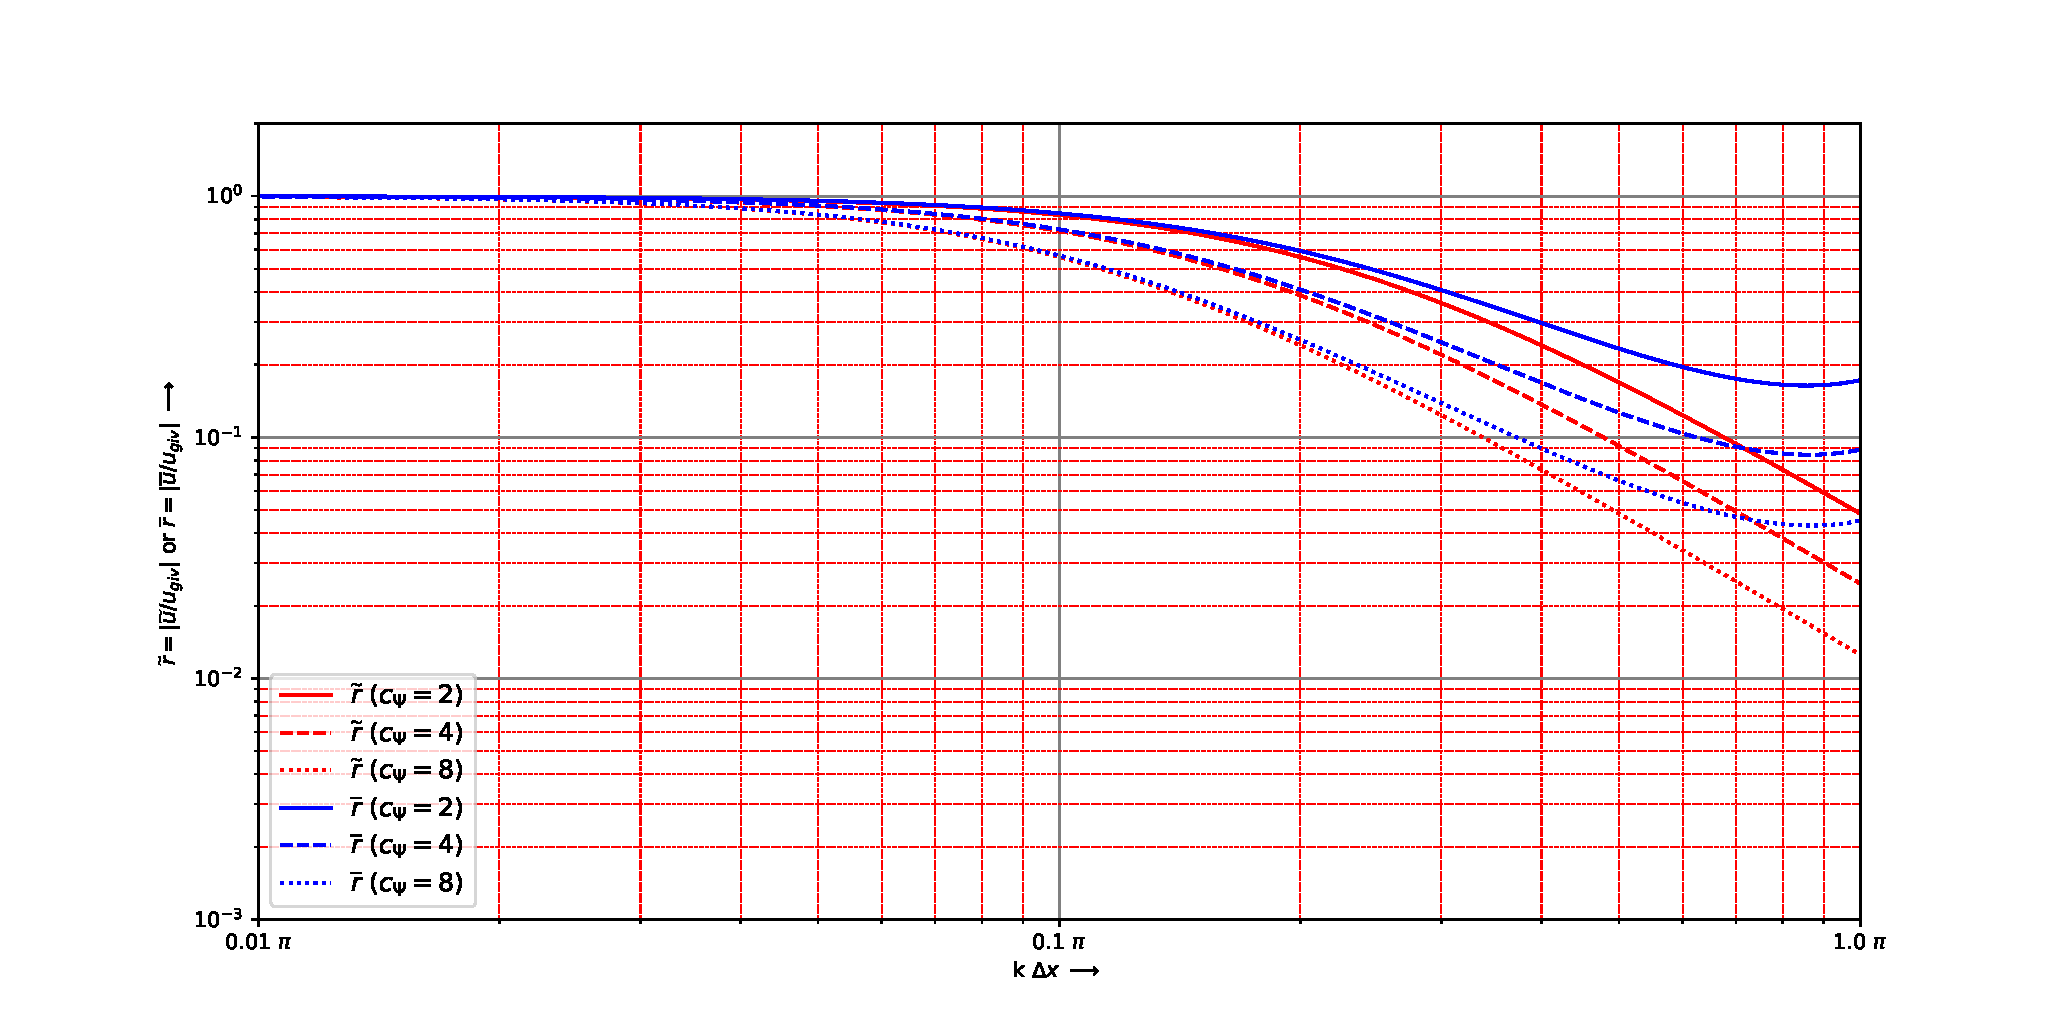
\includegraphics[width=0.99\textwidth]{figures/ratio_u_u_giv.pdf}
\caption{Ration between $\widetilde{r} = \abs{\widetilde{u}_k/u_{giv,k}}$ , and $\overline{r} = \abs{\overline{u}_k/u_{giv,k}}$. For different values of $c_{\Psi} = \Psi/\Dx^2$.\label{fig:ratio_func}}
\end{figure}
%--------------------------------------------------------------------------------
\section{Numerical error}
Discretization error values are determined when  $\Dx = {\it constant} $ and $\Psi = 0$, \autoref{eq:disc_regularization} reduces to:
\begin{align}
\frac{1}{8}      u_{i-1}
+ \frac{6}{8}   u_i
+ \frac{1}{8}   u_{i+1}  = \frac{1}{\Dx} \int_{x_{i-1/2}}^{x_{i+\half}} u_{giv}\, dx
\label{eq:disc_regularization_psi_0}
\end{align}

Numerical error as discretized between grid pints
\begin{align}
{\text{errorFVEgridpoint}}(k\Dx) = \abs{  1- \frac{8 \sin(\half  k\Dx)}{k\Dx  (3 + \cos(k\Dx))}}
\end{align}
Numerical error as discretized between cell centres (numerical Fourier-mode through the cell centres)
\begin{align}
{\text{errorFVEcellcentre}}(k\Dx) & = \abs{ 1 - \frac{8 \sin(\half k\Dx) \cos(\half k\Dx)}{k\Dx (3 + \cos(k\Dx))}}
\end{align}
With lowest order estimation of (see \citet{funcfitsmoothing_Fouriermodeanalysis2024}):
\begin{align}
-\frac{1}{24} (k\Dx)^2 - \frac{7}{960} (k\Dx)^4 + O(\Dx^6) % Computed with MapleSoft
\end{align}

So if the numerical error needs to be smaller then 1\ \%, the number of grid cells per wave length ($\lambda = N\Dx$) is computed as
\begin{align}
\frac{1}{24}(k\Dx)^2 < 0.01 \Rightarrow k\Dx < 0.5 \Rightarrow
\\
\left(\frac{2\pi}{N\Dx}\right)\Dx < 0.5 \Rightarrow N > 4\pi \approx 13
\end{align}
so per wave detail $\approx 7$ grid cells.

Discretization error values are given when  $\Psi = c_{\Psi}\Dx^2 = 0$ (see \autoref{fig:error_func}):
\begin{figure}[H]
\centering
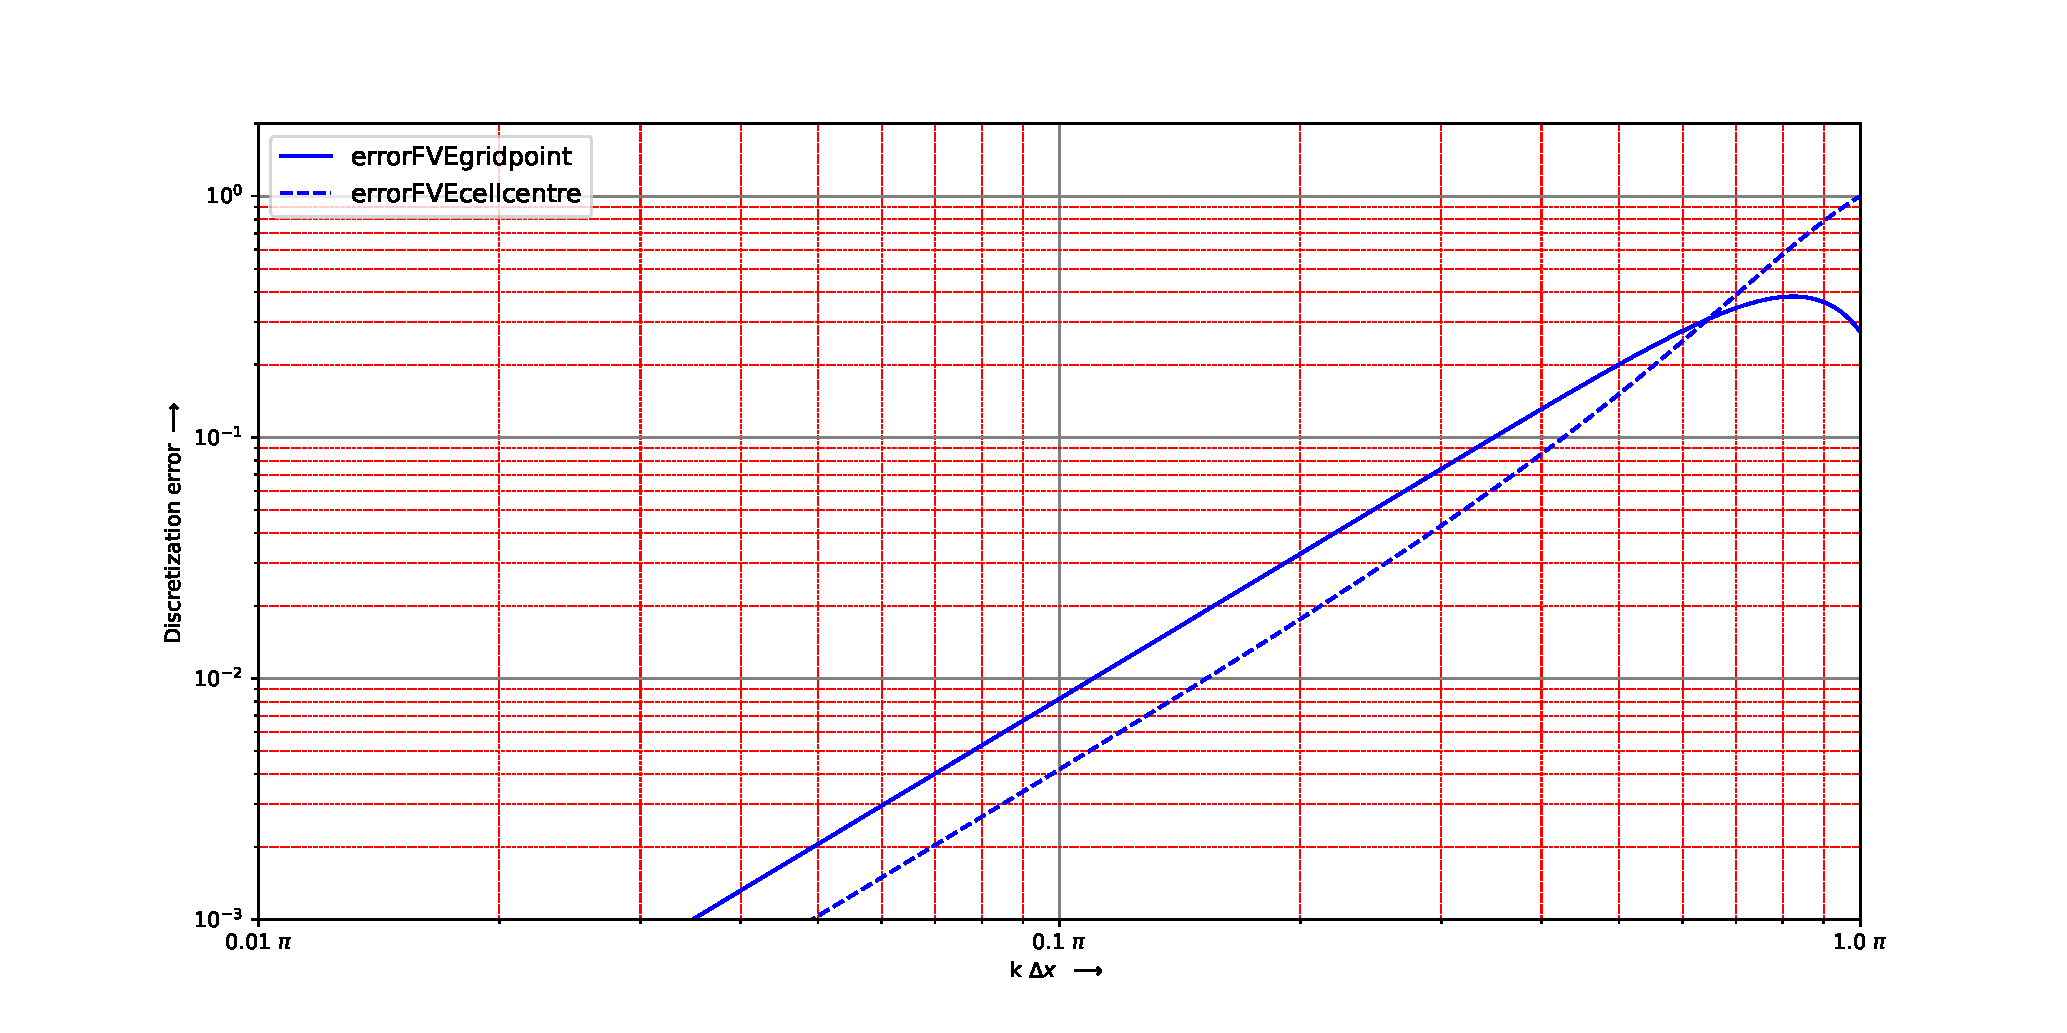
\includegraphics[width=0.99\textwidth]{figures/discr_error_u_u_giv.pdf}
\caption{Error function for value $\Psi = c_{\Psi}\Dx^2 = 0$. \label{fig:error_func}}
% python script: regularization_error_u_giv_u.py
\end{figure}

%-------------------------------------------------------------------------------
\section{Determining the factor $\mathbf{c_{\Psi}}$}\label{sec:determine_factor_c_psi}
In the limit of $k\Dx \rightarrow \infty$ \autoref{eq:r_tilde} behaves as:
\begin{align}
\lim_{k\Dx\to \infty}\frac{1}{1 + c_{\Psi}(k\Dx)^2} = \frac{1}{c_{\Psi}(k\Dx)^2}
\end{align}
The cut-off frequency is determined by $1 = 1/(c_{\Psi} (k\Dx)^2)$, hence filter parameter $c_{\Psi} = 1/(k\Dx)^2$ gives cut-off frequency $k$, or $k\Dx =\sqrt{1/c_{\Psi}}$ is obtained with filter parameter $c_{\Psi}$.
Given the wave length from the required numerical error (1\ \%, $N = 13$), the coefficient $c_{\Psi}$ reads:
\begin{align}
c_{\Psi} = \frac{1}{(k\Dx)^2} \quad \Rightarrow \quad c_{\Psi} = \frac{N^2 }{(2\pi)^2} \approx 4
\end{align}
%
%--- begin light blue table ---
\begin{longtable}{|>{\bfseries}p{6mm-12pt}|p{\textwidth/3-2mm-12pt}|p{\textwidth/3-2mm-12pt}|p{\textwidth/3-2mm-12pt}|}
\caption{Several typical values for numerical accuracy, $c_{\psi}$ and number of nodes per wavelength ($N$), the highligthed line is set as default.} \\%
 \rowcolor{mgreen1}
& {\textcolor{white}{\textbf{Accuracy}}}
& {\textcolor{white}{$\mathbf{c_{\Psi}}$}}
& {\textcolor{white}{$\mathbf{N}$}}
\\
\topline
\endfirsthead
\endhead
\endfoot
\bottomline
\endlastfoot
1 & 5\ \%   &  0.5 & 4.5\\
\midline
2 & 2\ \%  & 2    & 8.9 \\
\midline
\rowcolor{mgreen2} 3 & 1\ \%  &  4   & 12.8 \\
\midline
4 & 0.5\ \% & 10  & 18.1 \\
\end{longtable}
%--- end light blue table ---
%

%--------------------------------------------------------------------------------
\section{$L^1$-norm for the functions $\widetilde{u}$, $\overline{u}$ and $u_{\it given}$}
The next figures show the $L^1$-norm for the functions
$\abs{|\widetilde{u} - u_{\it giv}|}_{1}$,
$\abs{|\overline{u}  - u_{\it giv}|}_{1}$ and
$\abs{|\overline{u}  - \widetilde{u}|}_{1}$
\begin{figure}[H]
\begin{subfigure}{0.49\textwidth}
    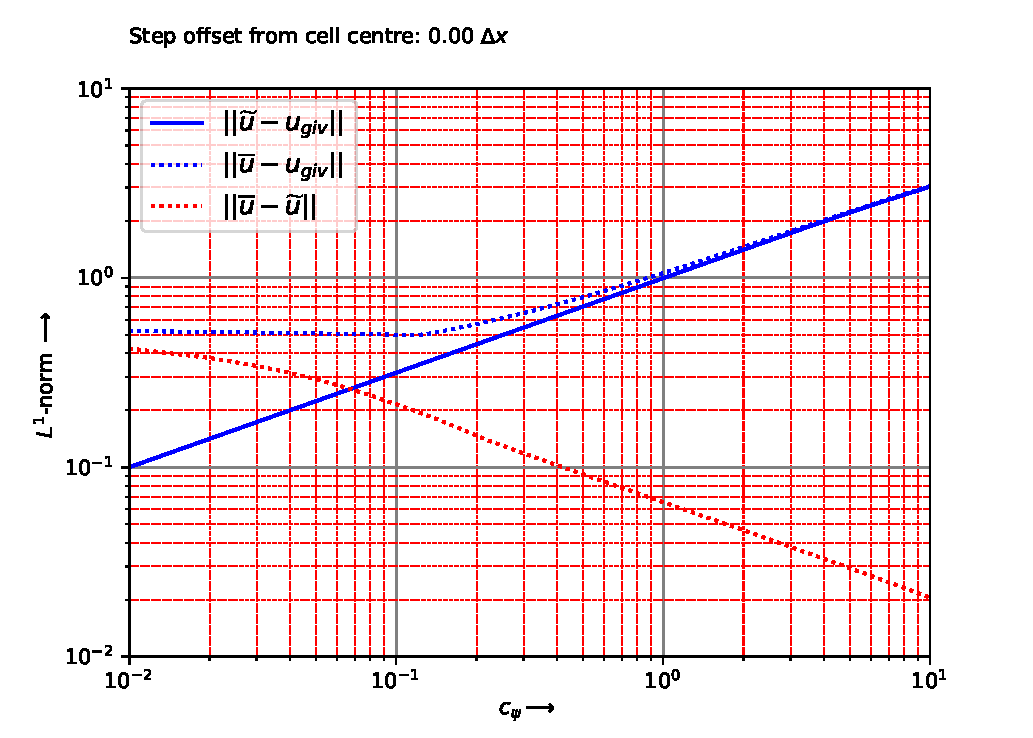
\includegraphics[width=\textwidth]{figures/regul_1d_step_at=0.0_dx50.0.pdf}
    \caption{Step defined at cell centre.\newline\phantom{text}\label{fig:L1_norm_dx_offset_0.0dx}}
\end{subfigure}
\hfill
\begin{subfigure}{0.49\textwidth}
    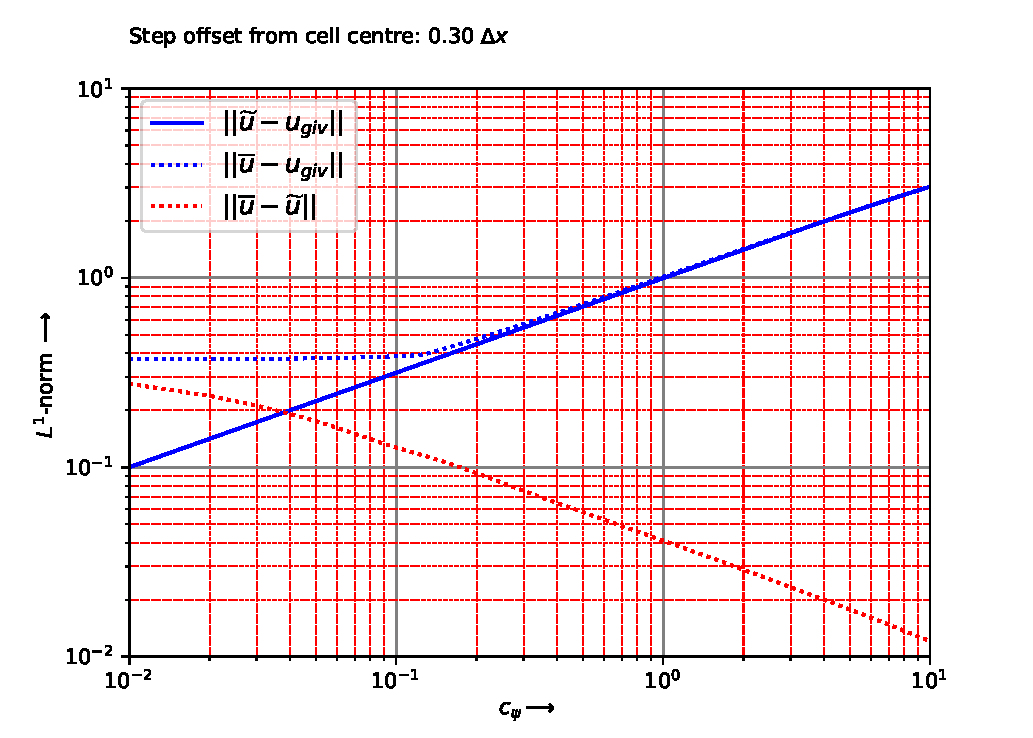
\includegraphics[width=\textwidth]{figures/regul_1d_step_at=0.3_dx50.0.pdf}
    \caption{Step defined with an off set of  0.3 $\Delta x$ from cell centre.\label{fig:L1_norm_dx_offset_0.3dx}}
\end{subfigure}
\\
\begin{subfigure}{0.49\textwidth}
    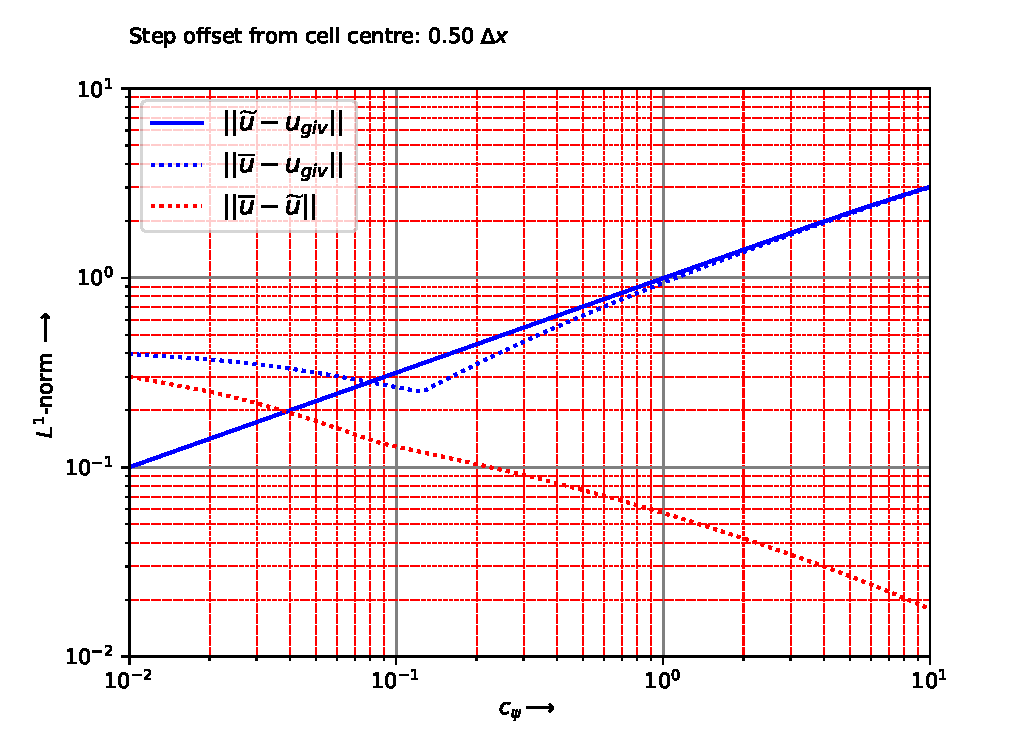
\includegraphics[width=\textwidth]{figures/regul_1d_step_at=0.5_dx50.0.pdf}
    \caption{Step defined with an off set of  0.5 $\Delta x$ from cell centre, thus defined at cell face.\label{fig:L1_norm_dx_offset_0.5dx}}
\end{subfigure}
\caption{Several plots of $L^1$-norm for different locations of the step.}
% Python script: reg_1d_step_less_error_when_more_smoothing.py
\end{figure}

As seen from these figures.
When choosing  $c_{\Psi} > 4$ then the $L^1$-norm of $\abs{|\overline{u} - \widetilde{u}|}_{1}$ is for all locations of the step smaller then $\num{2e-2}$ (red dotted lines in the plots).
Also the blue and blue dotted line are close together for $c_{\Psi}>4$.
That is the region in which we want to have the discetisation because there is the difference between the piecewise linear numerical solution $\overline{u}$ and the regularized solution $\widetilde{u}$ is independent of the location of the step, given by the function $u_{\it{giv}}$.

We also see that the dotted blue line is completely above the blue line if the step is located at the cell centre and with an offset of $0.3\Dx$ (see \autoref{fig:L1_norm_dx_offset_0.0dx} and \autoref{fig:L1_norm_dx_offset_0.3dx})
and it is partly below the blue line if the offset of the step is located at $0.5\Dx$ (\autoref{fig:L1_norm_dx_offset_0.5dx}).
The dotted blue line has also a sharp bend at the location where $c_{\Psi}=0.125$. These approximations are presented in the \autoref{fig:step_dx_offset_0.0dx}, \autoref{fig:step_dx_offset_0.3dx} and \autoref{fig:step_dx_offset_0.5dx}.
As seen from these plot the piecewise linear approximation shown in   \autoref{fig:step_dx_offset_0.5dx} is closer to the Heaviside function as the other two approximations.
\begin{figure}[H]
\begin{subfigure}{0.5\textwidth}
    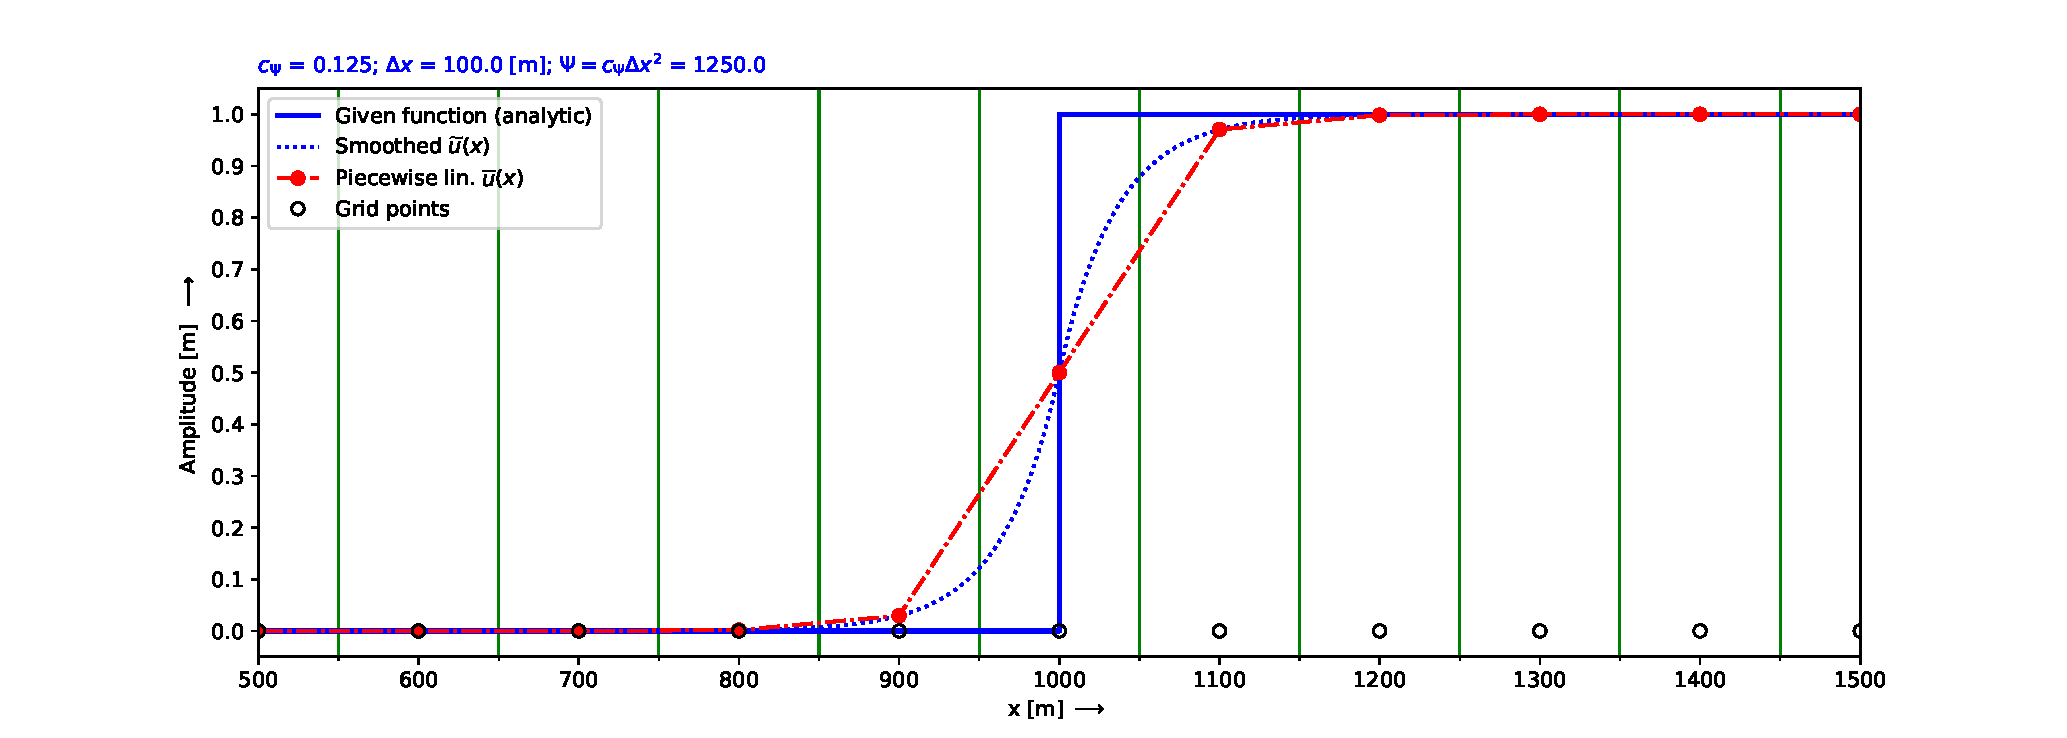
\includegraphics[width=\textwidth]{figures/regul_1d_step_at_0.00_function_dx100.0_cpsi0.125.pdf}
    \caption{Step defined at cell centre.\newline\phantom{text}\label{fig:step_dx_offset_0.0dx}}
\end{subfigure}
\begin{subfigure}{0.5\textwidth}
    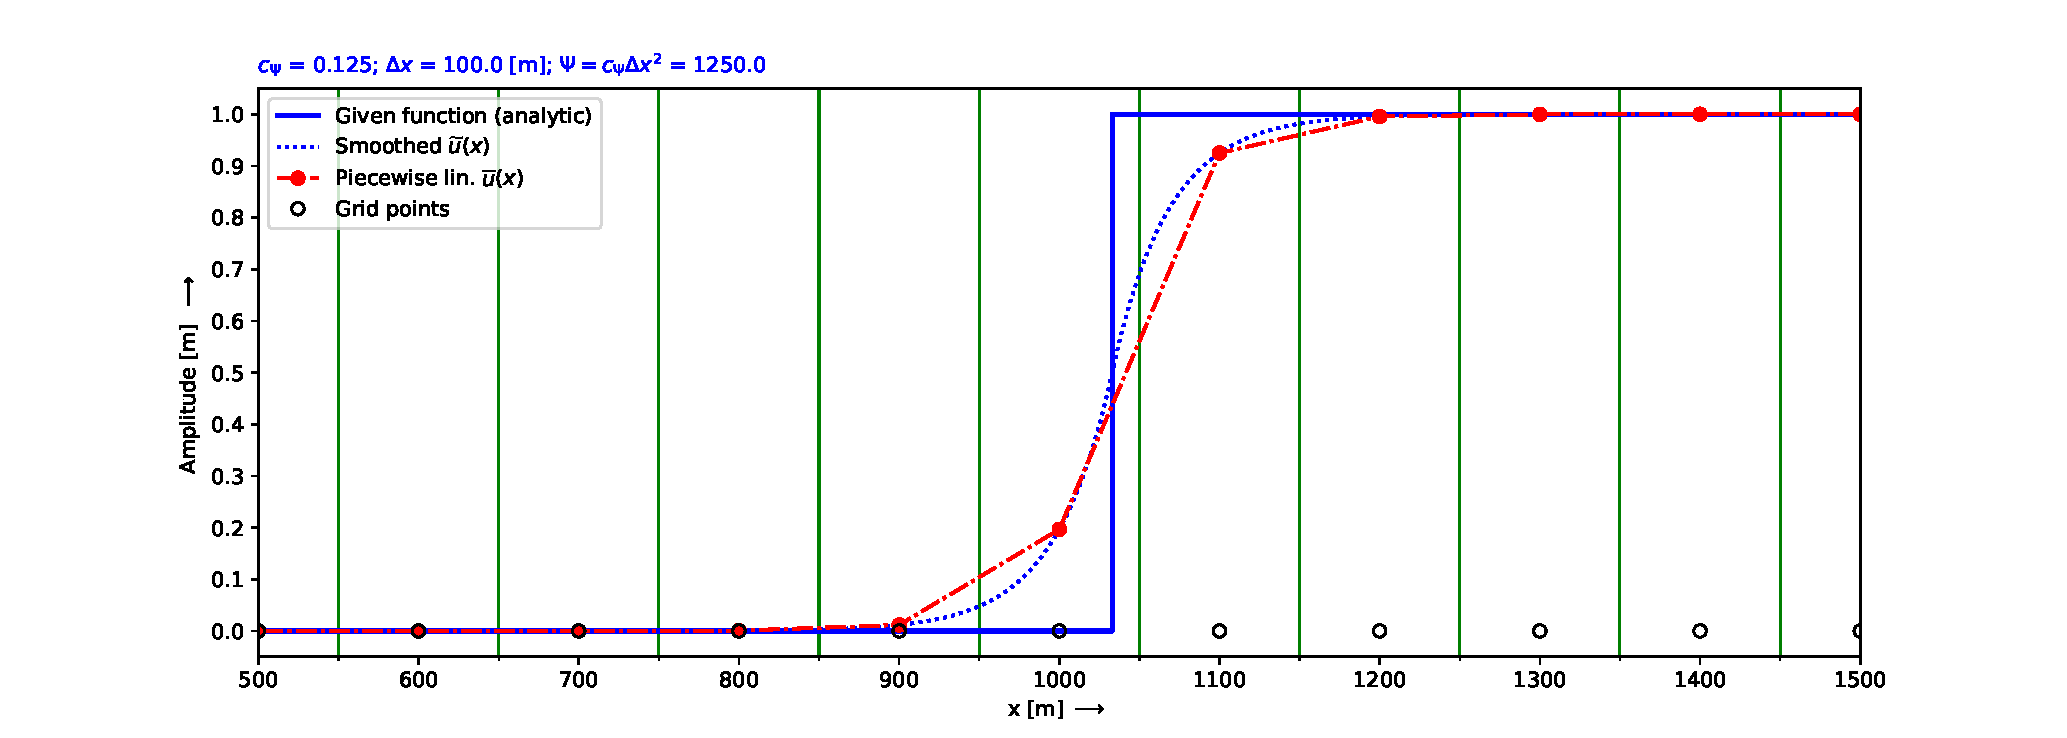
\includegraphics[width=\textwidth]{figures/regul_1d_step_at_0.33_function_dx100.0_cpsi0.125.pdf}
    \caption{Step defined with an of set of  0.3 $\Delta x$ from cell centre.\label{fig:step_dx_offset_0.3dx}}
\end{subfigure}
\newline
\begin{subfigure}{0.5\textwidth}
    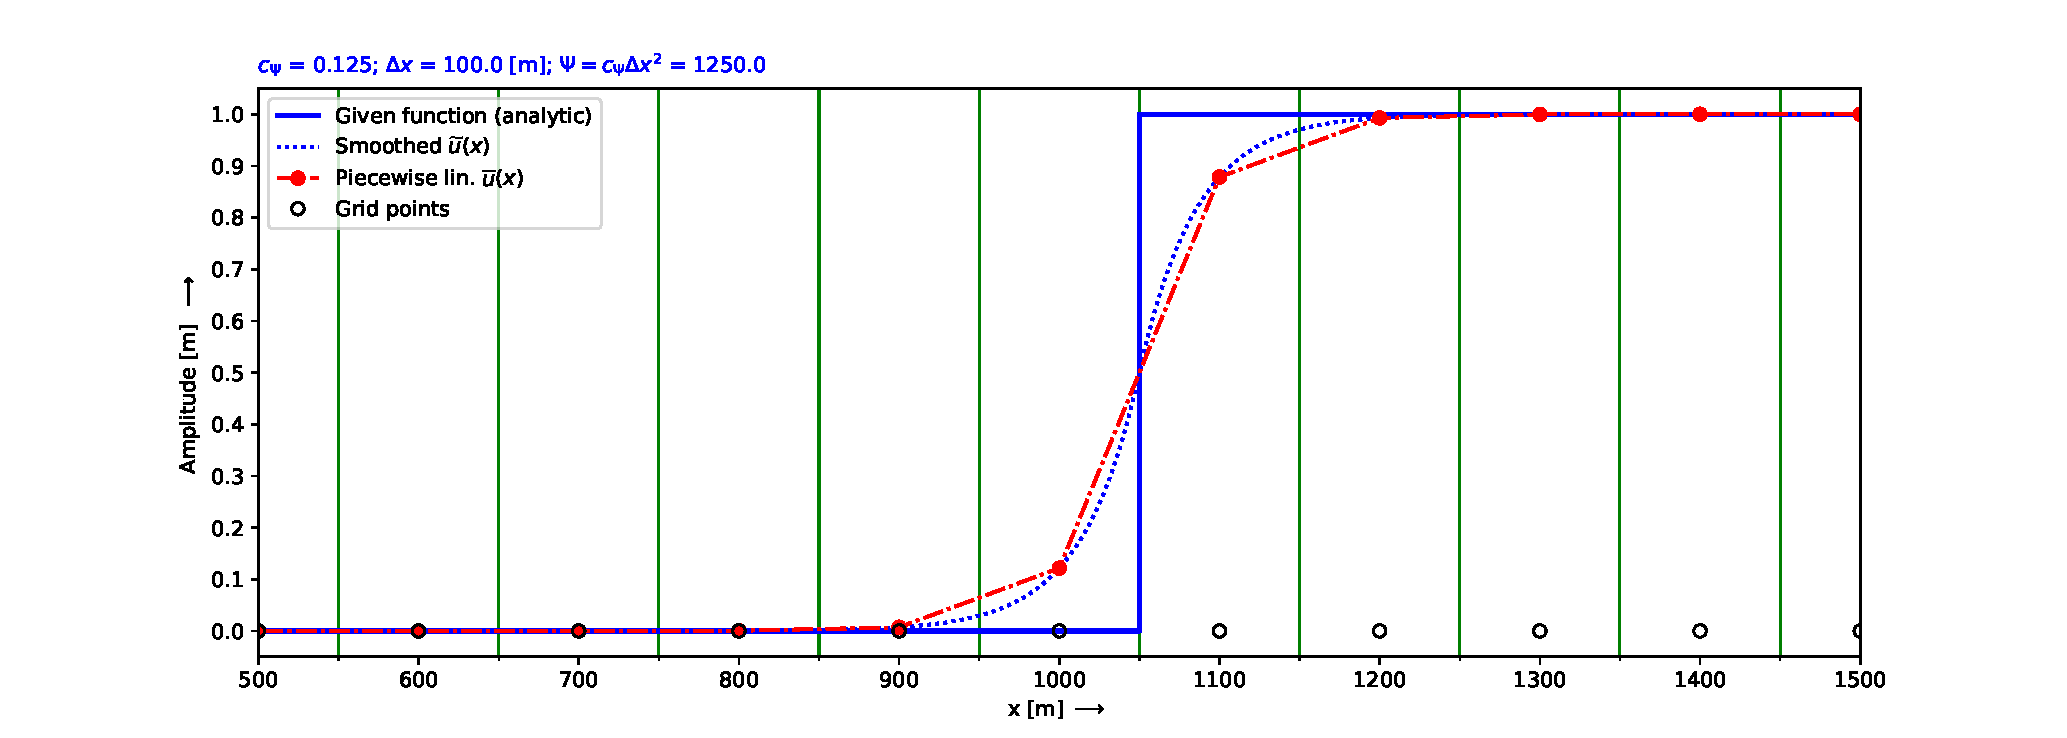
\includegraphics[width=\textwidth]{figures/regul_1d_step_at_0.50_function_dx100.0_cpsi0.125.pdf}
    \caption{Step defined with an of set of  0.5 $\Delta x$ from cell centre, thus defined at cell face.\label{fig:step_dx_offset_0.5dx}}
\end{subfigure}
\caption{Several plots of the piecewise linear approximation ($\overline{u}$) of the Heaviside function compared to the regularized function ($\widetilde{u}$).}
% Python script: reg_1d_step_less_error_1d_step_function.py
\end{figure}

%%--------------------------------------------------------------------------------
\chapter{Diagonalise 1-D wave equation with convection}\label{sec:diagonalise_conservative_wave_with_convection}

The one dimensional shallow water equations  with convection
read
%
\begin{align}
    \pdiff{h}{t}  + \pdiff{q}{x} & = 0 \label{eq:continuity_for_diagonalisation}\\
    \pdiff{q}{t}  + \pdiff{}{x} \left( \frac{q^2}{h} \right) + g h \pdiff{\zeta}{x} & = 0 \label{eq:momentum_for_diagonalisation}
\end{align}
Using $\zeta = h + z_b$ in the momentum equation the system of equations is written as:
\begin{align}
    \pdiff{h}{t}  + \pdiff{q}{x} & = 0
    \\
    \pdiff{q}{t}  + \pdiff{}{x} \left( \frac{q^2}{h} \right) + g h \pdiff{h}{x} & = -gh\pdiff{z_b}{x}
\end{align}
The convection term can rewritten in the linear form for the derivatives as:
\begin{align}
    \pdiff{}{x} \left( \frac{q^2}{h} \right) = \frac{2 q}{h} \pdiff{q}{x} - \frac{q^2}{h^2}\pdiff{h}{x}
    \label{eq:convection_linear_form}
\end{align}
In matrix notation it reads ($\zeta = h +z_b$ is used):
\begin{align}
    \begin{pmatrix} h \\ q \end{pmatrix}_t +
    \begin{pmatrix} 0 & 1  \\ gh-\frac{q^2}{h^2} & \frac{2q}{h} \end{pmatrix}
    \begin{pmatrix} h \\ q \end{pmatrix}_x =
    -gh \begin{pmatrix} 0 \\ z_b \end{pmatrix}_x
\end{align}
To make the system of equations diagonal, we have to find the eigen values and the eigen vectors.
The eigenvalues of the matrix are (using \maplesoft)
\begin{align}
    \lambda_1 = \frac{q}{h} + \sqrt{gh} \qquad \mbox{ and } \qquad
    \lambda_2 = \frac{q}{h} - \sqrt{gh}
\end{align}
The eigenvectors are
\begin{align}
    \begin{pmatrix} 1 \\ \frac{q}{h} + \sqrt{gh} \end{pmatrix}  \qquad \mbox{ and } \qquad
    \begin{pmatrix} 1 \\ \frac{q}{h} - \sqrt{gh} \end{pmatrix}
\end{align}
The diagonalised  SWE with convection read (after multiplying by $2\sqrt{gh}$, using  \maplesoft)
\begin{align}
    &\begin{pmatrix} \sqrt{gh} - \frac{q}{h} & 1  \\ \sqrt{gh} + \frac{q}{h} & -1 \end{pmatrix}
    \begin{pmatrix} h \\ q \end{pmatrix}_t +
    \begin{pmatrix} \frac{q}{h} + \sqrt{gh}   & 0  \\
        0 & \frac{q}{h} - \sqrt{gh}  \end{pmatrix}
    \begin{pmatrix} \sqrt{gh} - \frac{q}{h} & 1  \\ \sqrt{gh} + \frac{q}{h} & -1 \end{pmatrix}
    \begin{pmatrix} h \\ q \end{pmatrix}_x =
    \nonumber \\*
&= -gh \begin{pmatrix} \sqrt{gh} - \frac{q}{h} & 1  \\ \sqrt{gh} + \frac{q}{h} & -1 \end{pmatrix}
  \begin{pmatrix} 0  \\ z_b \end{pmatrix}_x
\end{align}
%
Written in two separate equations
\begin{align}
    &\left(\sqrt{gh} - \frac{q}{h}\right)\pdiff{h}{t} + \pdiff{q}{t} +  \left( \frac{q}{h} + \sqrt{gh}\right)\left( \left(\sqrt{gh} - \frac{q}{h} \right)\pdiff{h}{x} + \pdiff{q}{x} \right) =
    \nonumber \\*
    &\qquad = -gh\pdiff{z_b}{x} \quad \text{right going}
    \\
    &\left(\sqrt{gh} + \frac{q}{h}\right)\pdiff{h}{t} - \pdiff{q}{t} +  \left( \frac{q}{h} - \sqrt{gh}\right)\left( \left(\sqrt{gh} + \frac{q}{h} \right)\pdiff{h}{x} - \pdiff{q}{x} \right) =
    \nonumber \\*
    & \qquad = gh \pdiff{z_b}{x} \quad \text{left going}
\end{align}
First rearrange the equation for the right going wave (keep in mind that also \autoref{eq:convection_linear_form} is used):
\begin{align}
    &\left(\sqrt{gh} - \frac{q}{h}\right)\pdiff{h}{t} + \pdiff{q}{t} +
     \left( gh - \frac{q^2}{h^2} \right)\pdiff{h}{x} + \left( \frac{q}{h} + \sqrt{gh}\right) \pdiff{q}{x} = -gh\pdiff{z_b}{x}
     \\*
%    &\left(\sqrt{gh} - \frac{q}{h}\right)\pdiff{h}{t} + \pdiff{q}{t} +
% gh\pdiff{\zeta}{x} - \frac{q^2}{h^2}\pdiff{h}{x} + \left( \frac{q}{h} + \sqrt{gh}\right) \pdiff{q}{x} = 0
%     \\*
%&\left(\sqrt{gh} - \frac{q}{h}\right)\pdiff{h}{t} + \pdiff{q}{t} +
%gh\pdiff{\zeta}{x} - \frac{2 q}{h} \pdiff{q}{x} + \pdiff{}{x} \left( \frac{q^2}{h} \right) + \left( \frac{q}{h} + \sqrt{gh}\right) \pdiff{q}{x} = 0
%      \\*
 &\left(\sqrt{gh} - \frac{q}{h}\right)\left(\pdiff{h}{t} + \pdiff{q}{x}\right) + \left( \pdiff{q}{t} + \pdiff{}{x} \left( \frac{q^2}{h} \right) +
 gh\pdiff{\zeta}{x}\right)   = 0
\end{align}
and second, rearrange the equation for the left going wave:
\begin{align}
    &\left(\sqrt{gh} + \frac{q}{h}\right)\pdiff{h}{t} - \pdiff{q}{t} +  \left( \frac{q^2}{h^2} - gh\right)\pdiff{h}{x} - \left( \frac{q}{h} - \sqrt{gh}\right)\pdiff{q}{x} = gh \pdiff{z_b}{x}
     \\*
%    &\left(\sqrt{gh} + \frac{q}{h}\right)\pdiff{h}{t} - \pdiff{q}{t} +  \frac{q^2}{h^2}\pdiff{h}{x} - gh \pdiff{\zeta}{x} - \left( \frac{q}{h} - \sqrt{gh}\right)\pdiff{q}{x} = 0
%     \\*
%    &\left(\sqrt{gh} + \frac{q}{h}\right)\pdiff{h}{t} - \pdiff{q}{t} +  \frac{2 q}{h} \pdiff{q}{x} - \pdiff{}{x} \left( \frac{q^2}{h} \right) - gh \pdiff{\zeta}{x} - \left( \frac{q}{h} - \sqrt{gh}\right)\pdiff{q}{x} = 0
%     \\*
    &\left(\sqrt{gh} + \frac{q}{h}\right)\left(\pdiff{h}{t} + \pdiff{q}{x}\right)  - \left( \pdiff{q}{t} + \pdiff{}{x} \left( \frac{q^2}{h} \right) + gh \pdiff{\zeta}{x} \right) = 0
\end{align}
Which can be written as a combination of the continuity \eqref{eq:continuity_for_diagonalisation} and momentum equation \eqref{eq:momentum_for_diagonalisation} (see also \citet[eq.\ 4]{Borsboom2001}),
\begin{align}
    \begin{matrix}
    \quad \text{right going} \\
    \quad \text{left going}
\end{matrix}
\qquad
    \begin{pmatrix}
        \sqrt{gh} - \frac{q}{h}  &  1 \\
        \sqrt{gh} + \frac{q}{h}  &  -1
    \end{pmatrix}
    \begin{pmatrix} \textit{continuity eq.} \\ \textit{momentum eq.} \end{pmatrix}    = 0
\end{align}
or, after multiplying with $h$
\begin{align}
    \begin{matrix}
    \quad \text{right going} \\
    \quad \text{left going}
\end{matrix}
\qquad
    \begin{pmatrix}
        h\sqrt{gh} - q  &  h \\
        h\sqrt{gh} + q  &  -h
    \end{pmatrix}
    \begin{pmatrix} \textit{continuity eq.} \\ \textit{momentum eq.} \end{pmatrix}    = 0
\end{align}

%%--------------------------------------------------------------------------------
\chapter{Error function needed to regularize the artificial viscosity} \label{sec:error_artificial_viscosity}
%--------------------------------------------------------------------------------
Regularization of the artificial viscosity, assumed to be independent of time, is described in \autoref{sec:regularization_artificial_viscosity}.
The mentioned error-function is derived in this section and is based on \citet[eq.\ 42]{Borsboom2001}:

We start from the continuity and momentum equation for non-linear waves (i.e. \autoref{eq:continuity_equation} and \eqref{eq:momentum_equation} and combine these two equations to one equation representing the energy. 

The continuity and momentum equation read:
\begin{align}
    \pdiff{h}{t}  + \pdiff{q}{x} & = 0 \qquad \textit{continuity eq.} 
    \\
    \pdiff{q}{t}  + \pdiff{}{x} \left( \frac{q^2}{h} \right) + g h \pdiff{h}{x} & = 0 \qquad \textit{momentum eq.}
\end{align}
a suitable combination of these two equations yields the energy equation.
The suitable combination is:
\begin{align}
    \left( \half \frac{q^2}{h^2} + g \zeta\right)\left(\textit{continuity eq.}\right)  
    +
    \frac{q}{h} \left( \textit{momentum eq.} \right)= 0
\end{align}
and the energy equation reads:
\begin{align}
    \pdiff{}{t}\left( h \left(\half \frac{q^2}{h^2} + g \zeta - \half g h \right) \right) +
    \pdiff{}{x}\left( q \left( \half \frac{q^2}{h^2} + g\zeta  \right) \right)= 0
\end{align}
For a steady state solution ($q=\textit{Constant}$), when have:
\begin{align}
    &\pdiff{}{x}\left( \frac{1}{2} \frac{q^2}{h^2} + g\zeta  \right) = 
\frac{q}{h^2} \pdiff{q}{x} - \frac{q^2}{h^3}  \pdiff{h}{x} + g\pdiff{\zeta}{x} = 0
\end{align}
We assume that the artificial viscosity $\Psi$ proportional to the numerical error of the gradient term.

\notyet
%For stationary situations the artificial viscosity $\Psi$ is proportional the following equation:
%\begin{align}
%    &Err_\Psi = \Dxi\, \overline{x}_\xi \left( \half \sqrt{\frac{g}{\hbar}} \abs{D_\xi(\overline\zeta)} + 
%    \half \sqrt{2} \abs{\frac{D_\xi(\qbar)}{\hbar} - \frac{\qbar D_\xi(\hbar)}{\hbar^2}} \right)
%\end{align}
%Take the artificial viscosity $\Psi$ proportional to the numerical error of the gradient term, i.e.:
%\begin{align}
%    \Psi \propto \Dx \left( {\it Err} \abs{\sqrt{\half \frac{q^2}{h^2}}}  +  {\it Err} \abs{\sqrt{g\zeta}}  \right)
%\end{align}

%%--------------------------------------------------------------------------------
\chapter{Linearization in time}
%--------------------------------------------------------------------------------
\section{Viscosity term}\label{sec:linearisation_viscosity}
The viscosity term read:
\begin{align}
    &  \int^{x_{i+\half}}_{x_{i-\half}}\pdiff{}{x} \left( \nu h \pdiff{(q/h)}{x} \right)\ dx & =
    \left. \nu \left( \pdiff{q}{x} - \frac{q}{h} \pdiff{h}{x} \right) \right|_{x_{i+\half}} - \left. \nu \left( \pdiff{q}{x} - \frac{q}{h} \pdiff{h}{x} \right) \right|_{x_{i-\half}}
\end{align}
Linearization of the viscosity term at $x_{i+\half}$ read, where $\Delta h^{n+1, p+1} = \Delta h$ and  $\Delta q^{n+1, p+1} = \Delta q$:
\begin{align}
    &\left. \nu h \pdiff{(q/h)}{x} \right|^{n+\theta, p+1}  = \left. \nu \left(\pdiff{q}{x} - \frac{q}{h} \pdiff{h}{x} \right) \right|^{n+\theta, p+1} \approx
    \\
    & \approx \nu \pdiff{}{x} \left( q^{n+\theta, p} + \theta \Delta q \right)
    - \nu \frac{q^{n+\theta, p} + \theta \Delta q}{h^{n+\theta, p} + \theta \Delta h} \pdiff{}{x} \left( h^{n+\theta, p} + \theta \Delta h  \right) \approx
\end{align}
with
\begin{align}
    \frac{q^{n+\theta, p} + \theta \Delta q}{h^{n+\theta, p} + \theta \Delta h}
    & \approx \frac{q^{n+\theta, p} + \theta \Delta q}{h^{n+\theta, p}}\left( 1 - \frac{\theta\Delta h}{h^{n+\theta, p}} +
    \left( \frac{\theta\Delta h}{h^{n+\theta, p}}  \right)^2 - \left( \frac{\theta\Delta h}{h^{n+\theta, p}}  \right)^3 + \ldots \right) =
    \\
    & =
    \frac{q^{n+\theta, p}}{h^{n+\theta, p}} - \frac{q^{n+\theta, p}}{(h^{n+\theta, p})^2}\theta\Delta h + \frac{1}{h^{n+\theta, p}}\theta \Delta q  + O\left( \Delta q\Delta h, \left(\Delta h\right)^2 \right)
\end{align}
leaving out the terms of $O\left( \Delta q\Delta h, \left(\Delta h\right)^2 \right)$, yields:
\begin{align}
    &\left. \nu h \pdiff{(q/h)}{x} \right|^{n+\theta, p+1}  = \left. \nu \left(\pdiff{q}{x} - \frac{q}{h} \pdiff{h}{x} \right) \right|^{n+\theta, p+1} \approx
    \\
    & \approx \nu \pdiff{}{x} \left( q^{n+\theta, p} + \theta\Delta q  \right) +
    \\
    & \quad - \nu \left( \frac{q^{n+\theta, p}}{h^{n+\theta, p}} + \frac{1}{h^{n+\theta, p}}\theta\Delta q - \frac{q^{n+\theta, p}}{(h^{n+\theta, p})^2}\theta\Delta h   \right) \pdiff{}{x} \left( h^{n+\theta, p} + \theta\Delta h  \right) =
    \\
    & = \nu \pdiff{ q^{n+\theta, p}}{x}  + \nu \pdiff{}{x} \theta \Delta q +
    \\
    & \quad - \nu \frac{q^{n+\theta, p}}{h^{n+\theta, p}} \pdiff{h^{n+\theta, p}}{x} - \nu \frac{q^{n+\theta, p}}{h^{n+\theta, p}}\pdiff{}{x} \theta\Delta h - \frac{1}{h^{n+\theta, p}}\pdiff{h^{n+\theta, p}}{x} \theta\Delta q + \frac{q^{n+\theta, p}}{(h^{n+\theta, p})^2} \pdiff{h^{n+\theta, p}}{x} \theta\Delta h
\end{align}
rearranged
\begin{align}
    &\left. \nu h \pdiff{(q/h)}{x} \right|^{n+\theta, p+1}
    = \left. \nu \left(\pdiff{q}{x} - \frac{q}{h} \pdiff{h}{x} \right) \right|^{n+\theta, p+1} \approx
\\
    & = \nu \pdiff{ q^{n+\theta, p}}{x} - \nu \frac{q^{n+\theta, p}}{h^{n+\theta, p}} \pdiff{h^{n+\theta, p}}{x}  +
\\
    & \quad
    + \nu \theta \pdiff{\Delta q}{x}
    - \nu \theta \frac{1}{h^{n+\theta, p}}\pdiff{h^{n+\theta, p}}{x} \Delta q
    + \nu \theta \frac{q^{n+\theta, p}}{(h^{n+\theta, p})^2} \pdiff{h^{n+\theta, p}}{x} \Delta h
    - \nu \theta \frac{q^{n+\theta, p}}{h^{n+\theta, p}}\pdiff{\Delta h}{x}
\end{align}

%%--------------------------------------------------------------------------------
\chapter{Regularization of a two dimensional given function $u_{\it{giv}}$}
The regularization function read, based on \citet[eq.\ 6]{Borsboom1998}:
\begin{align}
    \widetilde{u} - \nabla \dotp \bPsi \nabla \widetilde{u} = u_{\it{giv}}, \qquad \bPsi = c_{\Psi}(\Delta x^2 + \Dy^2) E,
    \label{eq:regularization}
\end{align}
with $\bPsi$ the artificial viscosity and defined as:
\begin{align}
    \bPsi =
    \begin{pmatrix}
        \Psi_{11} & \Psi_{12} \\
        \Psi_{21} & \Psi_{22}
    \end{pmatrix}
\end{align}
where
\begin{symbollist}
    \item[$u_{giv}$] a given function, ex.\ bathymetry, viscosity, \ldots, [\si{\cdot}].
    \item[$\widetilde{u}$] Regularized/Smoothed function of $u_{giv}$, [\si{\cdot}].
    \item[$\Psi$] (artificial) smoothing constant, [\si{\square\metre}]
    \item[$\Dx, \Dy$] Space discretization, $\Dx_{i} = x_{i+\half} - x_{i-\half}$ and $\Dy_{j} = y_{j+\half} - y_{j-\half}$, [\si{\metre}]
    \item[$c_{\Psi}$] Smooting factor (set by user), [\si{1/\cdot}]
    \item[$E$] Error function, [\si{\cdot}]
\end{symbollist}
First the discretization of \autoref{eq:regularization} is discussed and second the determination of the artificial smoothing coefficient $\bPsi$.

Notation agreements:
\begin{symbollist}
    \item[$u$] Non-regularized/non-smoothed function, to be determined numerically.
    \item[$\widetilde u$] Regularized/smoothed function, denoted by the wavy line.
    \item[$\overline u$] Piecewise linear function, denoted by the bar.
    \item[$u_i$] Value of the numerical value at point $x_i$.
\end{symbollist}
%--------------------------------------------------------------------------------
\section{Discretization} % of \autoref{eq:regularization}}
The finite volume approach of this equation read:
\begin{align}
    \int_\Omega \widetilde{u}\, d\omega  - \int_\Omega \nabla \dotp \bPsi \nabla \widetilde{u}\, d\omega  = \int_\Omega  u_{\it{giv}}\, d\omega \label{eq:2d_regularization}
\end{align}

%--------------------------------------------------------------------------------
\subsection*{Integration of the first term}
The discretization of first term of \autoref{eq:2d_regularization} read
(see for the coefficients \autoref{fig:2d_structured_grid}):
\begin{align}
    \int_\Omega  u\, d\omega
    & \approx \Dx \Dy \Bigl( \frac{1}{64} u_{i-1,j-1} + \frac{6}{64} u_{i,j-1} + \frac{1}{64} u_{i+1,j-1} +
    \nonumber \\
    & + \frac{6}{64} u_{i-1,j} + \frac{36}{64} u_{i,j} + \frac{6}{64} u_{i+1,j} +
    \nonumber \\
    &  +\frac{1}{64} u_{i-1,j+1} + \frac{6}{64} u_{i,j+1} + \frac{1}{64} u_{i+1,j+1} \Bigl)
\end{align}
%--------------------------------------------------------------------------------
\subsection*{Integration of the second term}
Integration of the second term:
%
\begin{align}
    \int_\Omega & \nabla \dotp \bPsi \nabla \widetilde{u}\, d\omega  =
    \int_\Gamma \bPsi \nabla \widetilde{u} \dotp \vec{\hat n}\, ds \approx
    \\
    %
    & \approx
    \left. \frac{1}{2\Dy}\left( \Psi_{11} \pdiff{\widetilde{u}}{x} + \Psi_{12} \pdiff{\widetilde{u}}{y} \right) \right|_{i+\half,j-\quart}
    + \left. \frac{1}{2\Dy} \left( \Psi_{11} \pdiff{\widetilde{u}}{x} + \Psi_{12} \pdiff{\widetilde{u}}{y} \right) \right|_{i+\half,j+\quart} +
    \\
    &
    + \left. \frac{1}{2\Dx} \left( \Psi_{21} \pdiff{\widetilde{u}}{x} + \Psi_{22} \pdiff{\widetilde{u}}{y} \right) \right|_{i-\quart,j+\half}
    + \left. \frac{1}{2\Dx} \left( \Psi_{21} \pdiff{\widetilde{u}}{x} + \Psi_{22} \pdiff{\widetilde{u}}{y} \right) \right|_{i+\quart,j+\half} +
    \\
    &
    -  \left. \frac{1}{2\Dy} \left( \Psi_{11} \pdiff{\widetilde{u}}{x} + \Psi_{12} \pdiff{\widetilde{u}}{y} \right) \right|_{i-\half,j-\quart}
    -  \left. \frac{1}{2\Dy} \left( \Psi_{11} \pdiff{\widetilde{u}}{x} + \Psi_{12} \pdiff{\widetilde{u}}{y} \right) \right|_{i-\half,j+\quart}
    \\
    &
    - \left. \frac{1}{2\Dx} \left( \Psi_{21} \pdiff{\widetilde{u}}{x} + \Psi_{22} \pdiff{\widetilde{u}}{y} \right)  \right|_{i-\quart,j-\half}
    - \left. \frac{1}{2\Dx} \left( \Psi_{21} \pdiff{\widetilde{u}}{x} + \Psi_{22} \pdiff{\widetilde{u}}{y} \right)  \right|_{i+\quart,j-\half}
\end{align}
%
Define the components of $\bPsi$ at different locations with $(\mu, \nu) \in \{ 1, 2\}$ as
%
\begin{align}
    \left. \overline\Psi_{\mu\nu} \right|_{i+\half,j+\quart} = \frac{1}{8} \left(\left. 3\Psi_{\mu\nu} \right|_{i,j}
    + \left. 3\Psi_{\mu\nu} \right|_{i+1,j} + \left. \Psi_{\mu\nu} \right|_{i+1,j+1}  + \left. \Psi_{\mu\nu} \right|_{i,j+1}\right)
\end{align}
%
and define the partial differentials as
\begin{align}
    \left. \pdiff{u}{x} \right|_{i+\half,j+\quart} =  \quart \left(3\frac{u_{i+1,j} - u_{i,j}}{\Dx_{i+\half,j}} + \frac{u_{i+1,j+1} - u_{i,j+1}}{\Dx_{i+\half,j+1}}\right)
    \\
    \left. \pdiff{u}{y} \right|_{i+\half,j+\quart} =  \half \left(\frac{u_{i,j+1} - u_{i,j}}{\Dy_{i,j+\half}} + \frac{u_{i+1,j+1} - u_{i+1,j}}{\Dy_{i+1,j+\half}}\right)
\end{align}
%
In case the artificial viscosity is symmetric ($\Psi_{12} = \Psi_{21} = 0$) it reads:
%
\begin{align}
    \int_\Omega & \nabla \dotp \bPsi \nabla \widetilde{u}\, d\omega  =
    \int_\Gamma \bPsi \nabla \widetilde{u} \dotp \vec{\hat n}\, ds \approx
    \\
    %
    & \approx
    \left. \frac{1}{2\Dy}\left( \Psi_{11} \pdiff{\widetilde{u}}{x} \right) \right|_{i+\half,j-\quart}
    + \left. \frac{1}{2\Dy} \left( \Psi_{11} \pdiff{\widetilde{u}}{x} \right) \right|_{i+\half,j+\quart} +
    \\
    &
    + \left. \frac{1}{2\Dx} \left( \Psi_{22} \pdiff{\widetilde{u}}{y} \right) \right|_{i-\quart,j+\half}
    + \left. \frac{1}{2\Dx} \left( \Psi_{22} \pdiff{\widetilde{u}}{y} \right) \right|_{i+\quart,j+\half} +
    \\
    &
    -  \left. \frac{1}{2\Dy} \left( \Psi_{11} \pdiff{\widetilde{u}}{x} \right) \right|_{i-\half,j-\quart}
    -  \left. \frac{1}{2\Dy} \left( \Psi_{11} \pdiff{\widetilde{u}}{x} \right) \right|_{i-\half,j+\quart}
    \\
    &
    - \left. \frac{1}{2\Dx} \left( \Psi_{22} \pdiff{\widetilde{u}}{y} \right)  \right|_{i-\quart,j-\half}
    - \left. \frac{1}{2\Dx} \left( \Psi_{22} \pdiff{\widetilde{u}}{y} \right)  \right|_{i+\quart,j-\half}
\end{align}





In case the artificial viscosity is isotropic it reads:
\begin{align}
    \bPsi =
    \begin{pmatrix}
        \Psi & 0 \\
        0 & \Psi
    \end{pmatrix}
\end{align}
 (isotropic, $\Psi_{11} = \Psi_{22} = \Psi$ and $\Psi_{12} = \Psi_{21} = 0$).

The integration of the second  term will reduce to:
\begin{align}
    \int_\Omega & \nabla \dotp \bPsi \nabla \widetilde{u}\, d\omega  =
    \int_\Gamma \bPsi \nabla \widetilde{u} \dotp \vec{\hat n}\, ds =
    \Psi
    \int_{i-\half}^{i+\half} \int_{j-\half}^{j+\half} \nabla \widetilde{u} \dotp \vec{\hat n}\, dy dx
    \approx
    \\
    %
    & \approx
      \Psi \left(
      \left. \frac{1}{2\Dy} \pdiff{\widetilde{u}}{x}  \right|_{i+\half,j-\quart}
    + \left. \frac{1}{2\Dy} \pdiff{\widetilde{u}}{x}  \right|_{i+\half,j+\quart} +
    \right.
    \\
    &
    + \left. \frac{1}{2\Dx} \pdiff{\widetilde{u}}{y}  \right|_{i-\quart,j+\half}
    + \left. \frac{1}{2\Dx} \pdiff{\widetilde{u}}{y}  \right|_{i+\quart,j+\half} +
    \\
    &
    - \left. \frac{1}{2\Dy} \pdiff{\widetilde{u}}{x} \right|_{i-\half,j-\quart}
    - \left. \frac{1}{2\Dy} \pdiff{\widetilde{u}}{x} \right|_{i-\half,j+\quart}
    \\
    &
    \left.
    - \left. \frac{1}{2\Dx} \pdiff{\widetilde{u}}{y}   \right|_{i-\quart,j-\half}
    - \left. \frac{1}{2\Dx} \pdiff{\widetilde{u}}{y}   \right|_{i+\quart,j-\half}
    \right)
\end{align}
%--------------------------------------------------------------------------------
\subsection*{Integration of right hand side}
For the integration of the right hand side we could use a smaller integration step size, to incorporate the sub-grid scale effects.

%--------------------------------------------------------------------------------
\section{Determination of artificial smoothing coefficient $\Psi$}
The artificial smoothing coefficient (\autoref{eq:regularization}) is dependent on the second derivative of given function $u_{giv}$ \citep[eq.\ 8]{Borsboom1998}.
\textbf{Assuming} that $c_E$ is constant over the whole two dimensional area, thus isotropic.

\todo{Check next equations}

\begin{align}
        &  \Bigl( \frac{1}{64} E_{i-1,j-1} + \frac{6}{64} E_{i,j-1} + \frac{1}{64} E_{i+1,j-1} +
    \nonumber \\
    & + \frac{6}{64} E_{i-1,j} + \frac{36}{64} E_{i,j} + \frac{6}{64} E_{i+1,j} +
    \nonumber \\
    &  + \frac{1}{64} E_{i-1,j+1} +\frac{6}{64} E_{i,j+1} + \frac{1}{64} E_{i+1,j+1} \Bigl) +
    \nonumber \\
    &
    %
    c_E \left(
      \left. \frac{1}{2\Dy}  \pdiff{\widetilde{u}}{x}  \right|_{i+\half,j-\quart}
    + \left. \frac{1}{2\Dy}  \pdiff{\widetilde{u}}{x}  \right|_{i+\half,j+\quart} +
    \right. \\
    &
    + \left. \frac{1}{2\Dx}  \pdiff{\widetilde{u}}{y}  \right|_{i-\quart,j+\half}
    + \left. \frac{1}{2\Dx}  \pdiff{\widetilde{u}}{y}  \right|_{i+\quart,j+\half} +
    \\
    &
    - \left. \frac{1}{2\Dy}  \pdiff{\widetilde{u}}{x}  \right|_{i-\half,j-\quart}
    - \left. \frac{1}{2\Dy}  \pdiff{\widetilde{u}}{x}  \right|_{i-\half,j+\quart}
    \\
    &
    \left.
    - \left. \frac{1}{2\Dx}  \pdiff{\widetilde{u}}{y}   \right|_{i-\quart,j-\half}
    - \left. \frac{1}{2\Dx}  \pdiff{\widetilde{u}}{y}   \right|_{i+\quart,j-\half}
    \right)
    %
    =
    \nonumber \\
    & = \frac{1}{\Dx\Dy} \int_{j-\half}^{j+\half} \int_{i-\half}^{i+\half} \abs{D} \, dx\, dy
    \label{eq:error_regularization}
\end{align}
with \citep[eq.\ 2]{Borsboom1998}
\begin{align}
    D = \Dx^2 \pdiff[2]{u_{giv}}{x} + \Dy^2 \pdiff[2]{u_{giv}}{y}
\end{align}
and
\begin{align}
    c_E & = \max \left(  c_{\Psi}\Dx^2 \pdiff[2]{u_{giv}}{x},  c_{\Psi}\Dy^2 \pdiff[2]{u_{giv}}{y} \right)
    \nonumber \\
    & =  \max\left(
      c_{\Psi}\abs{u_{{giv}_{i-1,j}} -2 u_{{giv}_{i,j}} + u_{{giv}_{i+1,j}}},
      c_{\Psi}\abs{u_{{giv}_{i,j-1}} -2 u_{{giv}_{i,j}} + u_{{giv}_{i,j+1}}}
    \right), \forall i
\end{align}
The right hand side is approximated by:
\begin{align}
    & \frac{1}{\Dx\Dy} \int_{j-\half}^{j+\half} \int_{i-\half}^{i+\half} \abs{D} \, dx\, dy
    =
\nonumber \\
& \quad =  \frac{1}{64} \abs{D}_{i-1,j-1} +
\frac{6}{64} \abs{D}_{i,j-1} +
\frac{1}{64} \abs{D}_{i+1,j-1} +
\nonumber \\
    & \quad +
\frac{6}{64} \abs{D}_{i-1,j} +
\frac{36}{64} \abs{D}_{i,j} +
\frac{6}{64} \abs{D}_{i+1,j} +
\nonumber \\
& \quad + \frac{1}{64} \abs{D}_{i-1,j+1} +
\frac{6}{64} \abs{D}_{i,j+1} +
\frac{1}{64} \abs{D}_{i+1,j+1}
\end{align}

Now system \autoref{eq:error_regularization} can be solved and $\bPsi$ is set to:
\begin{align}
    \Psi = c_{\Psi}(\Dx^2 + \Dy^2) E
\end{align}
\end{document}